\documentclass[11pt,reqno]{amsart}
%% preamble.tex
\usepackage[T1]{fontenc}
\usepackage[utf8]{inputenc}
\usepackage{lmodern}
\usepackage[letterpaper,left=1.3in,right=1.3in,top=1.15in,bottom=1.15in,
  footskip=0.45in]{geometry}
\usepackage{amsmath,amssymb,amsthm,mathrsfs}
\usepackage{mathtools}
\usepackage[dvipsnames]{xcolor}
\usepackage{graphicx}
\usepackage{tikz}
\usetikzlibrary{arrows.meta,calc,positioning,decorations.pathmorphing,
  patterns,shapes.geometric,matrix,fit,backgrounds}
\usepackage{enumitem}
\usepackage{booktabs}
\usepackage{longtable}
\usepackage{array}
\usepackage{placeins}
\usepackage{microtype}
\usepackage[colorlinks=true,linkcolor=DeepBlue,citecolor=DeepBlue,
  urlcolor=DeepBlue,breaklinks=true]{hyperref}
\usepackage[capitalize,nameinlink]{cleveref}
\hypersetup{pdftitle={Explicit Base Points and Numerical Propagation for Weil
  Classes on Abelian Varieties},
  pdfauthor={Deep Bhattacharjee and Ushashi Bhattacharya},
  pdfkeywords={Hodge conjecture, Weil classes, semiregularity}}

\definecolor{DeepBlue}{RGB}{0,0,139}
\setlength{\emergencystretch}{3em}
\hbadness=3000
\raggedbottom
\interfootnotelinepenalty=0

%% ---------------------------------------------------------------- floats
\renewcommand{\topfraction}{0.92}
\renewcommand{\bottomfraction}{0.75}
\renewcommand{\textfraction}{0.06}
\renewcommand{\floatpagefraction}{0.72}

%% ---------------------------------------------------------- theorem envs
\theoremstyle{plain}
\newtheorem{theorem}{Theorem}[section]
\newtheorem{lemma}[theorem]{Lemma}
\newtheorem{proposition}[theorem]{Proposition}
\newtheorem{corollary}[theorem]{Corollary}
\newtheorem{conjecture}[theorem]{Conjecture}

\theoremstyle{definition}
\newtheorem{definition}[theorem]{Definition}
\newtheorem{example}[theorem]{Example}
\newtheorem{setupenv}[theorem]{Setup}
\newtheorem{question}[theorem]{Question}

\theoremstyle{remark}
\newtheorem{remark}[theorem]{Remark}
\newtheorem{notation}[theorem]{Notation}

\renewcommand{\qedsymbol}{$\blacksquare$}

\crefname{setupenv}{Setup}{Setups}
\Crefname{setupenv}{Setup}{Setups}

%% ------------------------------------------------------------- notation
\newcommand{\QQ}{\mathbb{Q}}
\newcommand{\ZZ}{\mathbb{Z}}
\newcommand{\RR}{\mathbb{R}}
\newcommand{\CC}{\mathbb{C}}
\newcommand{\PP}{\mathbb{P}}
\newcommand{\NN}{\mathbb{N}}
\newcommand{\Av}{A^{\vee}}
\newcommand{\cP}{\mathcal{P}}
\newcommand{\cF}{\mathcal{F}}
\newcommand{\cE}{\mathcal{E}}
\newcommand{\cG}{\mathcal{G}}
\newcommand{\cO}{\mathcal{O}}
\newcommand{\cL}{\mathcal{L}}
\newcommand{\cH}{\mathcal{H}}
\newcommand{\cI}{\mathcal{I}}
\newcommand{\cK}{\mathcal{K}}
\newcommand{\cA}{\mathcal{A}}
\newcommand{\cD}{\mathcal{D}}
\newcommand{\cV}{\mathcal{V}}
\newcommand{\cS}{\mathcal{S}}
\newcommand{\cX}{\mathcal{X}}
\newcommand{\cZ}{\mathcal{Z}}
\newcommand{\cQ}{\mathcal{Q}}
\newcommand{\Hdg}{\mathrm{Hdg}}
\newcommand{\HW}{W}                      % the Weil line
\newcommand{\NS}{\mathrm{NS}}
\newcommand{\Nm}{\mathrm{N}}             % the norm character
\newcommand{\cl}{\mathrm{cl}}
\newcommand{\Cn}{\mathrm{Cn}}
\newcommand{\bpf}{\mathrm{bpf}}

\DeclareMathOperator{\CH}{CH}
\DeclareMathOperator{\ch}{ch}
\DeclareMathOperator{\td}{td}
\DeclareMathOperator{\rk}{rk}
\DeclareMathOperator{\End}{End}
\DeclareMathOperator{\Hom}{Hom}
\DeclareMathOperator{\Ext}{Ext}
\DeclareMathOperator{\Pic}{Pic}
\DeclareMathOperator{\Hilb}{Hilb}
\DeclareMathOperator{\Res}{Res}
\DeclareMathOperator{\MT}{MT}
\DeclareMathOperator{\Hg}{Hg}
\DeclareMathOperator{\Gal}{Gal}
\DeclareMathOperator{\coker}{coker}
\DeclareMathOperator{\image}{im}
\DeclareMathOperator{\id}{id}
\DeclareMathOperator{\Spec}{Spec}
\DeclareMathOperator{\Supp}{Supp}
\DeclareMathOperator{\codim}{codim}
\DeclareMathOperator{\Sec}{Sec}
\DeclareMathOperator{\Tr}{Tr}
\DeclareMathOperator{\GU}{GU}
\DeclareMathOperator{\GL}{GL}
\DeclareMathOperator{\SL}{SL}
\DeclareMathOperator{\SU}{SU}
\DeclareMathOperator{\Sp}{Sp}
\DeclareMathOperator*{\colim}{colim}
\DeclareMathOperator{\ob}{ob}
\DeclareMathOperator{\Ann}{Ann}

\newcommand{\weightlattice}{\Lambda}
\newcommand{\Kx}{K^{\times}}
\newcommand{\bbar}[1]{\overline{#1}}
\allowdisplaybreaks[2]

\graphicspath{{figures/}}

\title[Base points and propagation for Weil classes]
      {Explicit Base Points and Numerical Propagation for Weil Classes on
       Abelian Varieties}

\author{Deep Bhattacharjee}
\address{Formerly, Electro-Gravitational Space Propulsion Laboratory (EGSPL),
  Bhubaneswar, Odisha 751030, India}
\email{d.bhattacharjee@erl-forschung.de}
\email{itsdeep@live.com}
\urladdr{\textnormal{ORCID
  \href{https://orcid.org/0000-0003-0466-750X}{0000-0003-0466-750X}}}

\author{Ushashi Bhattacharya}
\address{Formerly, National Taiwan University, Taipei 106319, Taiwan}
\email{rai.bhattacharya.in@gmail.com}
\urladdr{\textnormal{ORCID
  \href{https://orcid.org/0009-0002-2254-3914}{0009-0002-2254-3914}}}

\thanks{Deep Bhattacharjee is the corresponding author, at
\texttt{d.bhattacharjee@erl-forschung.de} and \texttt{itsdeep@live.com}.}

\thanks{Every numerical assertion in this paper is reproduced by the scripts
of \Cref{sec:verification}, which use exact rational, integer or exterior
algebra over $\QQ$ and no floating point at any step, and the finite
arithmetic on which the two main theorems turn is separately checked by the
Lean~4 kernel as described in \Cref{sec:lean}. Both are distributed with the
paper.}

\thanks{An earlier and substantially different version of part of this
material was posted by the authors on Preprints.org, on 5 August 2026, as
\emph{Relative Secant Cycles and Hodge Classes},
\href{https://doi.org/10.20944/preprints202602.0462.v5}%
{\texttt{doi:10.20944/preprints202602.0462.v5}}.
That version proposed a construction of algebraic representatives for Weil
classes. \Cref{thm:divisor,thm:character} below show that no construction of
that shape can produce a Weil class, and the present paper supersedes it. We
thank the referees of that version for pressing on the identification step,
which is where the obstruction lives.}

\date{\today}

\subjclass[2020]{Primary 14C30, 14K05;
  Secondary 14C25, 14D07, 14F08, 14J28, 11G10, 13D07, 32G20}

\keywords{Hodge conjecture, Weil classes, semiregularity}

\begin{document}

\begin{abstract}
Every family of abelian varieties of Weil type, of any field, dimension and
discriminant, contains a member whose Weil classes are explicit
polynomials in divisor classes, and its Hodge conjecture is the algebraicity
of one class on one connected period domain. Propagation from that member
would follow from a semiregular perfect complex carrying the Weil class. We
show that no complex whose Chern character is exactly a Weil class is
semiregular, in any dimension: it would deform to non-algebraic Weil tori,
where, extending a theorem of Voisin, coherent sheaves have no Chern character
below the top degree. The complex must also carry classes, such as powers of
the polarisation, that are Hodge only on the polarised family. Fourteen
further routes are closed. This route needs three further statements. The
last, the conjecture for varieties that are not abelian, is the whole
conjecture through $A\times\PP^{1}$; its form modulo abelian varieties holds
for varieties reached from abelian ones by correspondences and is open
beyond, and with it the route is one of five minimal routes found by
machine-checked computation. The Lefschetz standard conjecture holds
for the total space of every Mumford family. The first classes beyond the
Weil lines, on the square of a Mumford fourfold, are algebraic at every CM
point, rigid along the base curve, and represented by cycles at every closed
point of every reduction modulo a prime; they propagate to every member
exactly when it holds for one ninefold, or when those cycles have bounded
degree on a dense set, and once one complex has $\Ext^{2}$ of dimension
$119$.
\end{abstract}

\maketitle

\setcounter{tocdepth}{1}
\vspace*{-15pt}
\begingroup
\setlength{\parskip}{0pt}
\tableofcontents
\endgroup
\vspace*{-4pt}

\enlargethispage{4pt}
\section{Introduction}\label{sec:intro}

Let $X$ be a smooth complex projective variety. The Hodge conjecture asserts
that the cycle class map
\[
  \cl^{p}_{X}\colon \CH^{p}(X)_{\QQ}\longrightarrow \Hdg^{p}(X)
  \coloneqq H^{2p}(X,\QQ)\cap H^{p,p}(X)
\]
is surjective for every $p$. For $p=1$ this is the theorem of Lefschetz on
$(1,1)$ classes.%
\footnote{The rational coefficients are not a convenience. Lefschetz proved the integral statement in degree two, and the integral analogue in higher degree is false: Atiyah and Hirzebruch produced torsion classes of type $(p,p)$ that are not classes of cycles, and Koll\'ar later produced non-torsion ones. So the conjecture has to be stated after tensoring with $\QQ$, and every statement in this paper is a statement about $\QQ$-coefficients.} For $p\ge2$ the conjecture is open, and the two attacks that
are attempted most often are the following.

The first attack is algebraic and runs through abelian varieties. By the
structure theory of Hodge classes on abelian varieties, the Hodge ring of an
abelian variety of Weil type is generated by divisor classes together with
finitely many exceptional classes in middle degree, the Weil classes of
\cite{Weil77}.%
\footnote{Weil introduced them to show that the Hodge ring of an abelian variety is not always generated in degree one, which at the time was an open possibility. He did not conjecture that they are algebraic and did not claim they are not; the examples were offered as a warning, and they have been the standard test case ever since.} Divisor classes are algebraic, so for these varieties the whole
question is whether the Weil classes are algebraic. Markman
\cite{Mar25a,Mar25b} settled this for abelian sixfolds of Weil type of
discriminant $-1$, which are the sixfolds of split Weil type, for every
imaginary quadratic field, and deduced it for all abelian fourfolds of Weil type, for
every discriminant and every field, using a degeneration argument of Schoen
that he quotes; the Hodge conjecture for abelian varieties of dimension at
most five follows. The sheaf he produces has positive rank, is built from the
geometry of the abelian variety itself through a pair of secant sheaves on an
abelian threefold, and satisfies an equivariant semiregularity condition.%
\footnote{The hypothesis he verifies is stronger than injectivity of the
semiregularity map alone, and he asks in \cite[Question 11.4]{Mar25b} whether
it can be relaxed to injectivity on the image of an evaluation map, recording
in his Section 12 that an affirmative answer would carry the method to
abelian varieties of dimension at least eight and to fields of larger degree.
\Cref{cor:kernelfamily} below is a statement about the unrelaxed hypothesis;
\Cref{thm:weakfails} shows that for objects with Chern character concentrated
on the Weil line the relaxed hypothesis fails as well, by the same $n^{2}$
dimensions, and \Cref{prop:evaluation} that for the explicit split object of
\Cref{sec:construction} it fails by the whole kernel; \Cref{thm:linebundle}
that it fails for every object with a line bundle summand off the
polarisation line, at every member and in every dimension, so that no sum of
line bundles can run either argument (\Cref{cor:noline}); and
\Cref{rem:whatmeasures} says what remains, which is the positive rank,
indecomposable case the question was asked for. For that case
\Cref{thm:factor} computes the classes the relaxed hypothesis is about, for
every secant object on an abelian $n$-fold with $n\ge3$, and reduces the
hypothesis for Markman's own candidate in dimension eight to one identity
for a rank one complex on the fourfold; \Cref{thm:candidatefails} shows that
the identity fails, so that candidate does not satisfy the relaxed hypothesis
either.} For
$n\ge4$, and at $n=3$ for the discriminants not covered, the question is
open. It is natural
to hope that the higher cases can be reached by importing an object from an
ambient projective space, restricting it to the dual abelian variety, and
transporting the result to $A$ by the Fourier--Mukai transform. Secant
varieties of the dual are the usual choice of ambient object, because a
dimension count makes the codimension come out right.

The second attack is geometric and runs through induction on dimension. One
places the variety in a family of hyperplane sections, uses the algebraicity
of the Hodge locus \cite{CDK95} to control where the class stays of type
$(p,p)$, appeals to the conjecture in one dimension lower on the sections, and
attempts to transport the resulting cycles back up. Each ingredient here is a
theorem. The question is whether they compose.

This paper proves that neither attack can work, and it is precise about the
reasons, because the reasons are different in kind. The first fails for an
algebraic reason that no refinement of the construction can repair: the
classes the method produces live in the wrong subring, and they live there for
reasons of $\Kx$-equivariance that are visible before any geometry is chosen.
The second fails for a cohomological reason that is elementary once stated:
the restriction map annihilates exactly the classes the induction would need
to carry.

\subsection{The algebraic obstruction}

Throughout, $A$ is a complex abelian variety of dimension $g$, $\Av$ is its
dual, $\cP$ is the Poincar\'e bundle on $A\times\Av$, and
$\Phi_{\cP}\colon D^{b}(\Av)\to D^{b}(A)$ is the Fourier--Mukai transform with
kernel $\cP$. We write $\theta$ for a principal polarisation class on $A$ and
$\theta'$ for the dual class on $\Av$.

\begin{theorem}[Divisor obstruction]\label{thm:divisor}
Let $A$ be a principally polarised complex abelian variety of dimension $g$,
let $i\colon\Av\to\PP^{N-1}$ be any morphism defined by a linear system, and
let $\cF$ be any object of $D^{b}(\PP^{N-1})$. Put
$\cE=\Phi_{\cP}(Li^{*}\cF)$. Then
\[
  \ch_{k}(\cE)\in\QQ\cdot\theta^{k}\qquad\text{for every }k\ge0 .
\]
\end{theorem}

The proof has two ingredients and is short. The Chern character commutes with
derived pullback, which confines $\ch(Li^{*}\cF)$ to the subring of
$H^{*}(\Av,\QQ)$ generated by the hyperplane class, and the hyperplane class of
a linear system on an abelian variety is a multiple of $\theta'$. The
cohomological Fourier--Mukai transform then carries each power of $\theta'$ to
a rational multiple of a power of $\theta$; we prove this in closed form in
\Cref{thm:fmtheta}. Neither ingredient uses anything about $\cF$.

Since a Weil class is by construction not in the subring generated by divisor
classes, the consequence is immediate.

\begin{corollary}\label{cor:neverweil}
With notation as in \Cref{thm:divisor}, suppose in addition that $g=2n$ and
that $A$ is of $(K,-1,n)$-Weil type. Then $\ch_{n}(\cE)$ is a Weil class only
if $\ch_{n}(\cE)=0$.
\end{corollary}

We then give a second proof of \Cref{cor:neverweil} that does not pass through
\Cref{thm:divisor} and that explains, in representation-theoretic terms, why
the first proof had to succeed. The endomorphism $\iota(\tau)$ attached to
$\tau\in\Kx$ acts on $H^{2n}(A,\QQ)$, and the $\Kx$-isotypic decomposition of
that space separates the two objects in question.

\begin{theorem}[Character obstruction]\label{thm:character}
Let $(A,\iota,\eta)$ be of $(K,-1,n)$-Weil type and write
$H^{1}(A,\QQ)\otimes\CC=V_{+}\oplus V_{-}$ for the decomposition into
eigenspaces of $\iota(\sqrt{-d})$. Then
\[
  H^{2n}(A,\QQ)\otimes\CC
  =\bigoplus_{r+s=2n}\textstyle\bigwedge^{r}V_{+}\otimes\bigwedge^{s}V_{-},
\]
with $\iota(\tau)$ acting on the $(r,s)$ summand by
$\tau^{r}\bbar{\tau}^{\,s}$.
The Weil line $\HW(A)$ spans the two extreme summands $(r,s)=(2n,0)$ and
$(0,2n)$, on which $\Kx$ acts by $\tau^{2n}$ and $\bbar{\tau}^{2n}$, while
$\eta^{n}$ lies in the middle summand $(r,s)=(n,n)$, on which $\Kx$ acts by
the norm character $\Nm_{K/\QQ}(\tau)^{n}$. In particular, for every $n\ge1$,
\[
  \HW(A)\cap H^{2n}(A,\QQ)^{\Nm^{n}}=0,
\]
so a class that is a $\Kx$-eigenclass for $\Nm^{n}$ has zero component along
the Weil line.
\end{theorem}

\Cref{thm:character} is what makes the obstruction feel inevitable rather than
accidental. Any construction that is equivariant for the $K$-action, and
whose output is therefore an eigenclass, must choose a character in advance,
and the norm character is the one that the polarisation already occupies. The
Weil line sits at the two ends of the $\Kx$-grading, as far from the middle as
the grading allows. \Cref{fig:charactergrid} draws the grading and marks the
two positions.

It is tempting to look for a third obstruction of a numerical kind, and we
record in \Cref{sec:numerology} why there is none. A secant numerology
producing a class of codimension exactly $n$ on an abelian variety of
dimension $2n$ requires a polarisation on $\Av$ of Euler characteristic
$2n^{2}+2n$, which for $n\ge2$ is smaller than $2^{2n}$ and very much smaller
than $3^{2n}$. Those two quantities are the Euler characteristics at which
the theorem of Lefschetz guarantees that a linear system is free of base
points and that it is very ample, and it is easy to read them as thresholds
below which no such system exists. They are not. Both are sufficient
conditions and neither is necessary: an abelian surface with a polarisation of
type $(1,3)$ has $\chi=3<2^{2}$ and a base-point-free system, and one with a
polarisation of type $(1,5)$ has $\chi=5<3^{2}$ and a very ample system, the
latter being the Horrocks--Mumford embedding in $\PP^{4}$ \cite{HM73,GP98}. We
give the details in \Cref{sec:numerology}, because the erroneous reading
appears in an earlier version of part of this material and we wish to retract
it explicitly. Nothing else in the paper depends on it:
\Cref{thm:divisor,thm:character} are independent of any numerical count.

\subsection{The geometric obstruction}

The second half of the paper concerns induction on dimension. Let
$j\colon Y\hookrightarrow X$ be a smooth ample hypersurface in a smooth
projective variety of dimension $d$, and let $L=c_{1}(\cO_{X}(Y))$.

\begin{theorem}[Hyperplane obstruction]\label{thm:hyperplane}
Let $d=2p$ and let $\alpha\in H^{2p}(X,\QQ)$ be primitive. Then
$j^{*}\alpha=0$ for every smooth ample hypersurface $j\colon Y\hookrightarrow X$.
\end{theorem}

The proof is three lines from the projection formula and the Lefschetz
hyperplane theorem, and we give it in \Cref{sec:hyperplane}. Its force is that
the primitive middle degree is exactly where the Hodge conjecture is hard, and
it is exactly where the restriction map returns nothing. Below the middle
degree the restriction map is injective, but then the return trip is the
problem.

\begin{theorem}[The return trip]\label{thm:returntrip}
Let $2p\le d-2$, so that $j^{*}\colon H^{2p}(X,\QQ)\to H^{2p}(Y,\QQ)$ is an
isomorphism. If $j^{*}\alpha$ is algebraic on $Y$, then $L\alpha$ is algebraic
on $X$. The implication ``$L\alpha$ algebraic $\Rightarrow$ $\alpha$
algebraic'', asked of all smooth projective $X$ and all $\alpha$, is
equivalent to the Lefschetz standard conjecture.
\end{theorem}

Putting the two together gives the statement we want.

\begin{corollary}[No dimensional induction through hyperplane sections]%
\label{cor:noinduction}
Let $X$ be smooth projective of dimension $d$ and let $\alpha\in\Hdg^{p}(X)$.
An argument that deduces the algebraicity of $\alpha$ from the Hodge
conjecture for smooth ample hypersurfaces of $X$, using only $j^{*}$ and
$j_{*}$, returns no information when $2p=d$ and $\alpha$ is primitive, and
otherwise establishes the algebraicity of $L\alpha$ rather than of $\alpha$.
\end{corollary}

\Cref{sec:reduction} then states what is left. By hard Lefschetz every Hodge
class is determined by primitive classes in degrees at most $d$, and the
Lefschetz standard conjecture is the exact obstruction to moving between
degrees algebraically. The conclusion is a clean equivalence,
\Cref{thm:equivalence}: the Hodge conjecture holds for all smooth complex
projective varieties if and only if it holds for primitive classes of middle
degree and the Lefschetz standard conjecture holds. This is a restatement and
not a reduction, and we say so; its value is that it isolates the primitive
middle degree as the only place where new ideas can enter, and
\Cref{thm:hyperplane} says that the classical inductive handle is blind
precisely there.

\subsection{What is not obstructed}\label{ssec:introscope}

We are careful in \Cref{sec:scope} about the limits of these results, because
an obstruction theorem is only useful if its edges are sharp.

\Cref{thm:divisor} does not apply to Markman's construction \cite{Mar25a,Mar25b},
and \Cref{sec:escape} is devoted to saying exactly why, because that section is
the useful one for anybody who wants to build something new. In outline: a
rational class in the Weil line has a $\Kx$-orbit spanning a plane rather than
a line (\Cref{prop:orbitplane}), so any construction reaching it must be
bilinear in a pair of inputs interchanged by $\Gal(K/\QQ)$
(\Cref{cor:orbitcriterion}). Markman's construction is a secant construction,
and it satisfies this because it sites the secant geometry on an abelian
$n$-fold $X$, attaches two conjugate secant sheaves to the two points where a
plane of Hodge classes meets the spinor variety, and pairs them on
$X\times\widehat{X}$. The secant idea is therefore not what fails; siting it on
$\Av$ inside a projective space is what fails, and it fails three times over
(\Cref{prop:whichescaped}). \Cref{q:higher} states what an answer above the
known range would have to supply, and \Cref{sec:construction} supplies three
of its four ingredients in closed form for every $n$ and every $K$: the abelian
$2n$-fold of Weil type is $X\times\widehat{X}$ with a $K$-action written down
by one element of $\NS(X)$ (\Cref{thm:explicitweil}), and the plane is
$P_{t}=\QQ u_{t}\oplus\QQ v_{t}$ with $u_{t}$ and $v_{t}$ the even and odd
parts of $e^{\sqrt{-d}\,t}$ (\Cref{thm:plane}). The third ingredient becomes
an explicit equation: a secant sheaf has rank $a$, $c_{1}=bt$,
$c_{2}=\tfrac{ad+b^{2}}{2}t^{2}$, and Bogomolov discriminant equal to the norm
form $\Nm_{K/\QQ}(b+a\sqrt{-d})$ times $t^{2}$
(\Cref{thm:secantinvariants}), so the numerical obstruction vanishes
identically. At $n=3$ the equation forces the sheaf to be
$\mathcal{I}_{Z}(\Theta)$ with $Z$ a union of $d+1$ translates of the
Abel--Jacobi curve of a genus three Jacobian (\Cref{prop:genus3}), which is
the shape of the object used in \cite{Mar25b}. That equation is then solved in
every dimension. Because the secant plane has no preferred scale, one is free
to pass to a positive multiple of a rational point of it, and after clearing
denominators the Chern characters of the powers of a single line bundle already
span the subring $\QQ[t]$, the matrix that expresses them in the basis
$t^{k}/k!$ being a Vandermonde matrix. A class of positive rank on a smooth
projective variety is the class of a coherent sheaf, so the sheaf exists
(\Cref{lem:posrank} and \Cref{thm:secantexists}), with an explicit integer
witness in line bundles: at $n=4$, $d=3$ and $a=b=1$ the multiple is $6$ and
the witness is
$-23[\cO_{X}]+66[\cO_{X}(t)]-54[\cO_{X}(2t)]+20[\cO_{X}(3t)]-3[\cO_{X}(4t)]$.
The fourth ingredient, the deformation argument, is untouched, and
\Cref{rem:deformation} says so plainly; nothing here is a proof of the Hodge
conjecture at $n\ge4$, and \Cref{rem:thirdclosed} separates what has been
closed from what has not.

\Cref{thm:character} applies to any construction that is $K$-equivariant with
the norm character. A construction that is equivariant for the character
$\tau\mapsto\tau^{2n}$ would land in the right eigenspace, and we record in
\Cref{rem:rightcharacter} what such a construction would have to look like.
We do not know of one, and the difficulty is that $\tau\mapsto\tau^{2n}$ is
not $\QQ$-valued, so it cannot be realised by a correspondence defined over
$\QQ$ without additional structure.

\Cref{thm:hyperplane} concerns hyperplane sections. It does not obstruct
induction through other families, for instance through degenerations, through
blow-ups, or through the Kuga--Satake correspondence, which changes the
variety rather than cutting it. \Cref{sec:ks} sets that construction out in
full and marks its boundary. For a weight-two Hodge structure of K3 type it
transports the question to an abelian variety and turns the class into an
endomorphism, and \Cref{prop:ksnotrestriction} shows why nothing here bears on
it; but on an abelian variety of Weil type the hypothesis $h^{2,0}=1$ holds
only for $n=1$, by \Cref{prop:normpart}, and $n=1$ is exactly the case in
which the Weil line already consists of divisor classes.

\subsection{What the Weil classes look like, and how many there are}

Two further results are proved along the way, and they are the reason the
paper is longer than the first two obstructions require.

\Cref{thm:explicitgens} writes the Weil classes down. On the standard model of
an abelian variety of $(K,-1,n)$-Weil type, built in \Cref{sec:explicit} from
a $K$-vector space of dimension $2n$ and a hermitian form of signature
$(n,n)$, the Weil line has the integral basis
\[
  \omega_{1}=\sum_{|T|\ \mathrm{even}}(-1)^{|T|/2}d^{\,n-|T|/2}\,w^{(T)},
  \qquad
  \omega_{2}=\sum_{|T|\ \mathrm{odd}}(-1)^{(|T|-1)/2}d^{\,n-(|T|+1)/2}\,w^{(T)},
\]
where $T$ runs over the subsets of $\{1,\dots,2n\}$ and $w^{(T)}$ is the
monomial taking $y_{j}$ for $j\in T$ and $x_{j}$ otherwise. Each has $2^{2n-1}$
terms. Written this way the classes are objects one can compute with, and two
things become visible at once: the monomials occurring in them are disjoint
from those occurring in the powers of the polarisation, which gives an
elementary second proof of \Cref{prop:notpoly}; and the balanced signature in
the definition of Weil type is forced, since for any other signature the same
two classes are of type $(p,2n-p)$ and are not Hodge classes at all.

\Cref{thm:hdgcount} counts what is there. For $A$ of $(K,-1,n)$-Weil type with
$\Hg(A)=\SU(V,H)$,
\[
  \dim_{\QQ}\Hdg^{k}(A)=\begin{cases}3,&k=n,\\1,&k\ne n,\end{cases}
  \qquad
  \Hdg^{n}(A)=\QQ\,\eta^{n}\oplus\HW(A),
\]
so the Hodge conjecture for such an $A$, in every degree at once, reduces to
the algebraicity of the single class $\omega_{1}$. That is
\Cref{cor:whatisleft}, and it is what makes the obstruction theorems worth
proving: they are about one explicitly written class and not about a space of
unknown size.

\Cref{thm:divcriterion} then produces that class from divisors whenever a
certain condition holds. Write $R$ for the rational structure on
$\bigwedge^{2}V_{+}\oplus\bigwedge^{2}V_{-}$, the part of $H^{2}(A,\QQ)$ on
which $\Kx$ acts through $\tau^{2}$ and $\bbar{\tau}^{\,2}$. If $R$ contains a
Hodge class whose component in $\bigwedge^{2}V_{-}$ is a nondegenerate form
$\Theta$, then $\HW(A)$ is spanned by the real and imaginary parts of
$\Theta^{n}$, and these are polynomials in two divisor classes, hence
algebraic. On $A=X\times\widehat{X}$ with the $K$-action of
\Cref{sec:construction} the condition holds with
$\Theta=d\beta-\widehat{\beta}-\sqrt{-d}\,\ell$, which is
\Cref{thm:splitclosed}. \Cref{prop:divfails} shows the condition fails
whenever $\Hg(A)$ is the full special unitary group, so the criterion is
exactly a Noether--Lefschetz condition on $R$; and \Cref{prop:splitgeom}
determines what the split members supply: they have trivial discriminant,
whatever polarisation is chosen, they form a locus of codimension
$n(n-1)/2$, and at such a point the three classes
$\beta,\widehat{\beta},\ell$ already exhaust both the Neron--Severi group and
the Hodge classes in the middle degree.

\Cref{lem:Rendomorphism} identifies the criterion: a Hodge class in $R$ is the
same thing as an endomorphism $\mu$ with $\mu\iota(\tau)=\iota(\bbar{\tau})\mu$,
so the criterion asks for a quaternion algebra $(-d,\mu^{2})_{\QQ}$ inside
$\End^{0}(A)$ extending $K$. Those abelian varieties can be written down. For
$B=(-d,b)_{\QQ}$ with $b>0$ acting on $B^{n}$, \Cref{thm:quatweil} shows the
balanced signature is forced rather than imposed, computes the hermitian form
as $\mathrm{diag}(2a_{k}d,-2a_{k}bd)$, identifies the discriminant as the
class of $b^{n}$, and verifies the criterion with $\mu$ left multiplication by
$j$. Since $b$ may be any positive rational, and since discriminants multiply
over products, \Cref{thm:everyfamily} follows: every Weil family, for every
$K$, every $n$ and every discriminant, contains a member whose Weil classes
are algebraic, with a representative that is a polynomial in two divisor
classes. What is then left is propagation and nothing else, which is
\Cref{cor:R2}; and \Cref{cor:exactform} puts that in its sharpest form.
Deligne's theorem makes $\omega_{s}$ absolutely Hodge at every point, so the
Hodge conjecture for abelian varieties of Weil type, for every field, every
dimension and every discriminant, is equivalent to the single implication that
this one absolutely Hodge class is algebraic.

\subsection{What the last implication reduces to}

The set $\Sigma\subseteq\cD_{n,n}$ of points at which $\omega$ is algebraic is
then examined directly, in \Cref{ssec:properness}. Because the relative
Hilbert scheme is proper and the cycle class is locally constant in a flat
family, the part of $\Sigma$ cut out by one tuple of Hilbert polynomials is
Zariski closed; $\Sigma$ is the countable union of those pieces
(\Cref{thm:closedlocus}). Because algebraicity survives an isogeny and
$\SU(V,H)$ acts trivially on the Weil line, $\Sigma$ is stable under
$\SU(V,H)(\QQ)$, and that group has dense orbits, so $\Sigma$ is dense
(\Cref{prop:densealg}). The two facts together give a dichotomy with nothing
between its halves: either $\Sigma$ is everything, and the Hodge conjecture
holds for all abelian varieties of Weil type in the family, or $\Sigma$ has
empty interior and the conjecture fails outside a meagre set
(\Cref{cor:allornothing}).

One further operation preserves $\Sigma$, and it is the only one that moves
between dimensions. If $A_{1}$ and $A_{2}$ are of Weil type for the same $K$,
with parameters $n_{1}$ and $n_{2}$, then $A_{1}\times A_{2}$ is of Weil type
with parameter $n_{1}+n_{2}$, and the Weil class of the product is a fixed
rational combination of external products of the Weil classes of the factors
(\Cref{thm:weilmult}). Written in terms of the $K$-valued invariant
$\omega=\omega_{1}+\sqrt{-d}\,\omega_{2}$ the combination is simply
$\omega(A_{1})\omega(A_{2})=2\,\omega(A_{1}\times A_{2})$, so the Weil class is
multiplicative and algebraicity passes from the factors to the product
(\Cref{cor:prodalg}). At $n=1$ the Weil classes lie in $H^{2}$ and are
therefore algebraic by Lefschetz with no hypothesis at all, so taking $n$
abelian surfaces of Weil type gives, in every dimension and for every $d$, an
abelian $2n$-fold of Weil type whose Weil classes are written as an explicit
integral polynomial in $2n$ divisor classes (\Cref{thm:everyn}). That is the
only statement in this paper which produces an algebraic Weil class in every
dimension while quoting nothing, and its reach is correspondingly small: the
locus of such products has dimension $n$ inside a family of dimension $n^{2}$,
smaller even than the quaternionic locus, and a general member of the family
is simple and lies on none of them (\Cref{rem:prodscope}).

That is what turns the last implication into two statements of finite
character, each about the cycles already constructed. \Cref{thm:degreebound}:
if the Hilbert data of the cycle of \Cref{thm:everyfamily}, transported along
one rational orbit, takes finitely many values, the conjecture follows for the
whole family; at $n=2$, where the quaternionic locus is a divisor, infinitely
many repetitions suffice rather than all but finitely many
(\Cref{rem:ntwo}). \Cref{thm:semiregclosure}: the base point carries a perfect
complex whose Chern character is $N\omega_{1}$ in degree $n$ and zero
elsewhere (\Cref{prop:ktheory}), and if its semiregularity map is injective,
the conjecture again follows for the whole family. Of the two, the second
cannot be run on the object that supplies it: by
\Cref{prop:concentrated} the complex of \Cref{prop:ktheory} has
semiregularity kernel of dimension at least $n^{2}$ at every base point
constructed here, so its hypothesis fails for the object that supplies it
(\Cref{rem:killsreduction}), and by \Cref{cor:kernelfamily} the kernel is a
canonical copy of the tangent space to the family the deformation was to
cross, so no choice of base point inside the family can improve it. The degree bound is untouched, and \Cref{prop:leadingconstant} sharpens
it: the leading coefficient of the Hilbert polynomial is constant along the
orbit, because $G(\QQ)$ preserves both the Weil class and the polarisation,
so what has to be bounded is only the degree of the effective part of the
transported cycle (\Cref{rem:whereunbounded}). The divisorial constructions
cannot supply that bound: products of effective divisors of bounded degree
represent $\omega$ only on a nowhere dense set (\Cref{prop:divroute}), and
\Cref{prop:pencil} shows the degrees growing along an explicit pencil of
quaternionic loci in one fixed polarised lattice. Neither reduction mentions
a general point and neither assumes the variational Hodge conjecture; the
passage from a formal deformation at one point to cycles everywhere, which is
the part that is usually missing, is supplied by \Cref{thm:closedlocus}. We
have not proved either hypothesis, and \Cref{rem:tworemain} says exactly what
each of them asks for.

\Cref{ssec:whatobject} then says what the object of the second criterion has
to be. For a sum of line bundles the semiregularity map is computed in closed
form (\Cref{lem:splitsemireg}): it annihilates every off-diagonal extension
class and the traceless part of every diagonal one, so injectivity forces
multiplicity one, a vanishing of cohomology that the shifts can arrange, and
the injectivity of $(\zeta_{i})\mapsto\sum_{i}e^{\lambda_{i}}\zeta_{i}$.
The Chern character condition then fails outright.
\Cref{thm:positivity}: at any member whose only divisor classes of norm
character are the multiples of $\eta$, if the Chern character of an object is
an effective combination $\sum_{i}m_{i}e^{\lambda_{i}}$ of exponentials of
divisor classes and $\ch_{2}$ is a flat Hodge class, then the coefficient of
$\theta^{+}\theta^{-}$ is $\sum_{i}m_{i}\Nm_{K/\QQ}(u_{i})$ and must vanish;
the norm form is positive definite and the $m_{i}$ are positive, so every
$u_{i}$ is zero and the Weil component of the Chern character is zero as
well. The separation of $\theta^{+}\theta^{-}$ from $\eta^{2}$ that this
needs is \Cref{lem:tensorrank}, and it is a statement about tensor rank: in
the isotypic component for the square of the norm character the first class
has rank one and the second has rank $\binom{2n}{2}$.

The hypothesis on the Chern character holds for every sheaf filtered by line
bundles, for every semi-homogeneous bundle in the sense of Mukai
\cite{Muk78}, and for every iterated extension of those; the hypothesis on
the divisor classes holds at every split member and at every quaternionic base
point. So the candidates one would reach for first do not exist, and the
reason is positivity rather than a computation. What is left must be
indecomposable in the derived category with a class in $K_{0}$ that is not
effective, which is a sharper description of the remaining construction than
we started with.

The same subsection then asks where such an object could live at all, and the
answer is arithmetic. Writing the candidate as a sum of line bundles indexed
by elements $u_{i}$ of the ring of integers of $K$, the Chern character
conditions become $T_{q,r}=\sum_{i}m_{i}u_{i}^{q}\bbar u_{i}^{\,r}=0$ for all
$q,r\le n$ but three, and grouping the $u_{i}$ by norm turns the diagonal part
of that system into $\sum_{j}M_{j}N_{j}^{r}=0$ for $r=1,\dots,n$, where
$N_{1}<\dots<N_{\nu}$ are the norms that occur and $M_{j}$ is the sum of the
multiplicities at level $N_{j}$. Fewer than $n+1$ norms forces every $M_{j}$
to vanish and the rank with it (\Cref{cor:nplusone}); at exactly $n+1$ the
level sums are forced by Lagrange interpolation, and since multiplicity one
allows each element of the ring only once, they are capped by the number of
elements of each norm. \Cref{thm:pterange} runs that competition to the end.
For $4\le n\le8$, six imaginary quadratic fields and norms up to the bounds in
\Cref{sec:verification}, no set of norms meets the two demands, so in that
range the split route closes before any geometry is used. At $n=3$ it does
not: exactly eleven sets of four norms survive, all at $d=1$ or $d=2$, and the
smallest of them is $(9,18,27,36)$ over $\QQ(\sqrt{-2})$, where the level sums
are $(4,-6,4,-1)$ and the object would have rank one. For all eleven the rest
of the system is then shown to have no solution, by an exhaustive search over
sign patterns that covers $4.29\times10^{14}$ cases in the largest instance.

\subsection{Verification}

Every numerical claim in this paper is checked by exact arithmetic, and the
output is reproduced in \Cref{app:scripts}. The scripts verify the closed form
of the cohomological Fourier--Mukai transform on powers of $\theta$, the
stability of $\QQ[\theta]$ under the transform, the numerical question of
\Cref{cor:nonumerical} for $2\le n\le8$, the identity
$\sum_{q}h^{q,q+2}=\binom{4n}{2n-2}$ for the semiregularity target of
\Cref{sec:semireg}, the character separation of \Cref{thm:character}, the
coordinate model and the two generators \eqref{eq:omegagens}, the invariant
count behind \Cref{thm:hdgcount}, the Clifford arithmetic of \Cref{sec:ks},
and the family and secant plane of \Cref{sec:construction}. All arithmetic is
over $\QQ$ or in the exterior algebra of a finite-dimensional vector space
with integer structure constants; no step is numerical in the floating-point
sense. \Cref{sec:lean} describes a second, independent check of the finite
arithmetic by the Lean~4 kernel.

\subsection{Organisation}

\Cref{sec:conventions} fixes conventions. \Cref{sec:weiltype} develops the
structure theory of abelian varieties of Weil type from the definitions,
\Cref{sec:explicit} writes the Weil classes out in coordinates and counts the
Hodge classes, and \Cref{sec:characters} proves \Cref{thm:character}.
\Cref{sec:fm} establishes the closed form of the cohomological Fourier--Mukai
transform, and \Cref{sec:divisor} proves \Cref{thm:divisor} and
\Cref{cor:neverweil}. \Cref{sec:numerology} settles the numerical question in
the negative, and \Cref{sec:semireg} computes the semiregularity target,
explains why it is not the binding constraint either, and then proves
\Cref{thm:rankzero}: no object whose Chern character is concentrated on the
Weil line is semiregular, because the annihilator of the Weil line in
$H^{0,2}$ has dimension $n^{2}$ (\Cref{lem:annihilator}). It then identifies
that annihilator: by \Cref{thm:anntangent} the polarisation carries the
tangent space to the Weil family isomorphically onto it, and by
\Cref{prop:firstorder} a polarisation-preserving deformation kills the whole
Weil line exactly when it commutes with $K$, so the family is also the
first-order Hodge locus of the class. The kernel and the family are therefore
the same space, which is \Cref{cor:kernelfamily}; and \Cref{thm:weakfails}
places that space inside the image of the evaluation map of Hochschild
cohomology, so that the weakened semiregularity criterion of
\cite[Question 11.4]{Mar25b} is unavailable for such objects too; and
\Cref{thm:linebundle} shows, from the infinitesimal rigidity of divisor
classes, that any object with a line bundle summand off the polarisation
line is obstructed along the family in a direction the semiregularity map
cannot see, which removes every sum of line bundles in every dimension. This
is the fourth obstruction, and it is the one that bears directly on the
fourth ingredient of \Cref{rem:deformation}. \Cref{sec:hyperplane}
proves \Cref{thm:hyperplane} and \Cref{thm:returntrip}, and \Cref{sec:ks}
marks the boundary of the one classical route that gets past them.
\Cref{sec:reduction} proves the equivalence, \Cref{sec:escape} identifies which
hypotheses a construction must break, and \Cref{sec:construction} gives a
family of examples in which three of the four ingredients are supplied in
closed form, settles the base case in every family, and closes with
\Cref{ssec:properness} on the structure of the algebraic locus and
\Cref{ssec:whatobject} on the object the second criterion requires, where
\Cref{prop:splitobstruction} computes the first-order obstruction of the
explicit split object against the family: it is nonzero exactly in the
directions normal to the split locus, it lies in the kernel of the
semiregularity map, and it is transverse to the copy of the tangent space
that \Cref{cor:kernelfamily} places there; and \Cref{prop:evaluation} writes
out the evaluation map of Hochschild cohomology on that object and finds that
the whole kernel of the semiregularity map is in its image; and
\Cref{prop:markman8} computes the Chern character of Markman's candidate
object in dimension eight, places it at the point $(1,3)$ of the secant
plane, and reduces its verification to one condition on one sheaf; and
\Cref{thm:factor} moves that condition from the eightfold to the fourfold,
by computing the Hochschild classes that preserve any secant Chern
character, $n^{2}$ of them, so that the weakened criterion for the transform
of $\cF\boxtimes\cF$ becomes the single identity
$\mathrm{At}(\cF)^{2}=-d\Theta^{2}\cdot\id$ in
$\Ext^{2}(\cF,\cF\otimes\Omega^{2})$ for $\cF$ itself
(\Cref{cor:markmancondition}); and \Cref{thm:candidatefails} decides that
identity in the negative, by a local computation at an isolated double point
of the support, so that the candidate of Markman's Section 12 does not
satisfy the weakened criterion, and \Cref{cor:localobstruction} extends the
obstruction to every dimension. What that argument cannot reach is a support
with no such point, and \Cref{ssec:smoothsupport} takes up that case. At a
smooth point the sheaf $\cE xt^{2}$ of the ideal vanishes, so both sides of
the identity are locally zero and the germ comparison has nothing to compare
(\Cref{prop:smoothlocal}); the question moves from a point to the normal
bundle. In exchange the surface itself becomes rigid. Since the Todd class of
an abelian variety is trivial, Grothendieck--Riemann--Roch turns the Chern
character into the whole numerical package of the support, and for
$\ch(\cF)=u_{\Theta}+b\,v_{\Theta}$ on a fourfold it gives
\[
  \chi(\cO_{S})=(b^{2}+d)(3b^{2}-d),\quad
  K_{S}^{2}=3(b^{2}+d)(7b^{2}-d),\quad
  e(S)=3(b^{2}+d)(5b^{2}-3d),
\]
with nothing left free. Because $\Omega^{1}_{S}$ is a quotient of the trivial
bundle $\Omega^{1}_{X}|_{S}$, it is globally generated, so $K_{S}$ is nef and
$e(S)\ge0$; then $K_{S}$ is also big, $S$ is minimal of general type, and the
Bogomolov--Miyaoka--Yau inequality applies. Its defect is
$3e(S)-K_{S}^{2}=24(b^{4}-d^{2})$, so the inequality says exactly $d\le b^{2}$
(\Cref{thm:smoothinvariants}). At the value $b=3$ that the fourfold forces,
this leaves $d\in\{1,3,5,7\}$ (\Cref{cor:fourdiscriminants}): for every
imaginary quadratic field beyond those four there is no secant object of rank
one with smooth support at all, and for those four the invariants are the
six numbers of \Cref{tab:smoothsupport} and nothing else.
The same subsection then identifies what the local argument is really testing.
It is not smoothness and it is not the complete intersection property: at any
point where the support is Cohen--Macaulay the sheaf $\cE xt^{2}$ of its ideal
vanishes, because Auslander--Buchsbaum makes the ideal of projective dimension
one there, so both sides of the identity are locally zero
(\Cref{thm:cmvanishing}). A Macaulay2 computation over ten germs confirms the
line, and shows it is sharp: the fat plane and the cone over the twisted cubic
are not complete intersections and still carry no obstruction, while two
planes meeting at a point, three planes meeting pairwise at a point, and a
plane with an embedded point all do. So the criterion splits cleanly
(\Cref{cor:cmdichotomy}): a support that is not Cohen--Macaulay is removed
outright, and a support that is Cohen--Macaulay has no local obstruction at
all, leaving one global vanishing in
$H^{1}(Z,\cE xt^{1}(\cI_{Z},\cI_{Z}))$. That also explains why Markman's
candidate cannot be repaired by normalising its double points: separating the
branches is what restores the depth, and \Cref{rem:normalisationcm} shows it
moves the Chern character off the secant plane.
A Cohen--Macaulay support of codimension two has an ideal sheaf of projective
dimension one, by the same Auslander--Buchsbaum argument, so it is resolved by
two vector bundles of ranks $r+1$ and $r$. That is a shape one can search.
\Cref{ssec:hilbertburch} does so. When the two bundles are sums of line
bundles the Chern character condition becomes four equations on the twists,
and at $r=1$, the complete intersections, they close outright for every $b$
and every $d$: weighting by $w(x)=x^{2}+d$, which is positive because $d>0$,
turns three of the equations into the statement that two positive measures
share their mass, mean and variance, and a one atom measure has variance zero,
so the two divisor degrees would have to coincide and the resolution would
cancel (\Cref{thm:noci}). At $r=2$ and $r=3$ an exact search over the twists
finds nothing either. At $r=4,5,6$ solutions appear, but only at $d=15$ and
$d=23$ (\Cref{thm:burchsearch}). None of them survives: a morphism from a
secant object that satisfies the criterion to a power of the polarisation is
killed by $H^{2}(\cO)$ (\Cref{lem:annihilation}), and for the cone of a map
between sums of such powers the summand inclusions are not, because the
relevant $H^{2}$ of a nontrivial power vanishes; so no split resolution runs
the criterion at any rank, any twist or any discriminant
(\Cref{thm:nosplit}), and the same holds when the line bundles are replaced
by simple semi-homogeneous bundles, the bundles with scalar Atiyah class
(\Cref{thm:noblocks}). What remains is a support that is either smooth, with
$d$ one of four values, or singular and Cohen--Macaulay, in both cases with a
Hilbert--Burch resolution over a bundle that is not projectively flat and a
restriction $H^{2}(\cO_{X})\to H^{2}(\cO_{Z})$ that is injective
(\Cref{cor:disjointroutes}). \Cref{rem:routemap} writes the two remaining
questions in the form a construction would have to answer.
Before that, \Cref{sec:cmfields} removes the restriction to quadratic
fields. The four theorems that turn the conjecture for a Weil family into a
propagation statement, namely the reduction to one class, the closedness of
the algebraic locus, the density of the rational orbits and the base point,
use nothing about the degree of the field. Carrying them over needs one new
input, a base point, and we supply it for every CM field $F$ of degree $2m$,
every $n$ and every discriminant: the abelian variety is isogenous to a
product of CM abelian $m$-folds, the Weil classes there are polynomials with
rational coefficients in $F$-balanced divisor classes, written out in
\Cref{thm:cmbasepoint}, and they are algebraic by the Lefschetz theorem on
$(1,1)$ classes. The density of the rational orbits needs the hermitian form
to be isotropic over the totally real subfield, which the Hasse principle
gives, and then the unipotent radicals of the parabolic subgroups generate
(\Cref{thm:cmpropagation}). So the Weil classes of the higher CM fields are
not a separate problem standing beside the quadratic ones: they are the same
propagation problem, and the semiregularity criterion, met at one base point
of each family, closes all of them at once. Nothing in that section is conditional on Question 11.4 or on any
secant construction.
\Cref{ssec:closuremap} then sets down, once and in full, what separates all of
this from the conjecture, and \Cref{ssec:closure} decides which parts of it
matter. The implications proved here, together with those the literature
supplies, form a finite rule set, and taking consequences in that rule set is
a computation rather than a judgement. The conjecture is not among the
consequences, which is the machine statement that nothing here proves it.
The route that passes through this paper needs three open statements: a
propagation statement, the one established in \Cref{thm:semiregclosure} and
carried to every CM field in \Cref{thm:cmpropagation}, and by
\Cref{prop:descent} needed only for the split families of the CM fields of
degree at least four, together with the
Hodge classes on abelian varieties that divisor and Weil classes do not
generate, and the conjecture for the varieties that are not abelian
(\Cref{cor:fourremain}). The last of the three is not a remainder: the
varieties that are not abelian include $A\times\PP^{1}$ for every abelian
variety $A$, and the conjecture for $A\times\PP^{1}$ gives it for $A$, so
that statement is equivalent to the whole conjecture (\Cref{prop:f3ishc}).
The statement that belongs in its place is weaker: every Hodge class is
algebraic modulo the images of Hodge classes of abelian varieties under
algebraic correspondences (\Cref{def:f3prime}). It holds on every variety
whose cohomology is reached from abelian varieties in that way, a class
containing curves and abelian varieties and closed under products and
surjective images, in degrees $0$, $2$, $2n-2$ and $2n$, and in dimension at
most three (\Cref{prop:f3prime}); beyond that it is open, and its standard
open case, the square of a K3 surface, turns on the same Kuga--Satake
correspondence as the Mumford classes below (\Cref{rem:f3primeopen}). With
both statements in the rule set there are exactly five minimal sets of open
statements that yield the conjecture (\Cref{thm:closure}). Two are the
conjecture restated: the conjecture for the varieties that are not abelian
alone, and the Lefschetz standard conjecture for every variety together with
the motivatedness of every Hodge class (\Cref{prop:lefmot}). The other three
use the weaker statement, together with the Lefschetz standard conjecture,
with the variational Hodge conjecture for algebraic classes that it implies
(\Cref{prop:lefvhc}, \Cref{thm:vhcab}), or, along the route of this paper,
with the propagation statement and the classes that divisor and Weil classes
do not generate. Only that last route uses a theorem of this paper. Every
statement in the five except the propagation statement is a consequence of
the conjecture, and the Lefschetz standard conjecture, which lies in two of
them and gives the whole abelian half, is the target at the centre
(\Cref{rem:bullseye}). None
of these statements is proved here in general. One new case of the Lefschetz
standard conjecture is: for an abelian scheme over a curve whose invariant
cycles are algebraic, the operator $\Lambda$ is the sum of a relative
Pontryagin product with $\ell^{g-1}/(g-1)!$ and an operator along the base
built from the invariant cycles, so it is algebraic; this covers the total
space of every Mumford family (\Cref{prop:pontryaginlambda},
\Cref{thm:lefschetzfamily}, \Cref{cor:mumfordlefschetz}). The same
decomposition shows that, for such a total space, the Lefschetz standard
conjecture is exactly the statement that algebraicity propagates along the
curve (\Cref{thm:lefschetzpropagation}). With the base points of this paper
that turns each of the two remaining targets into the Lefschetz standard
conjecture for one variety: one Weil family is equivalent to it for the
total space of the family over a curve through a base point
(\Cref{cor:weilequiv}), and the first classes beyond the Weil lines are
equivalent to it for the ninefold $W\times_{C}W$ of a Mumford family
(\Cref{cor:mumfordequiv}). Two statements are proved outright on the way:
the Hodge conjecture for $X_{c}\times X_{c}$ at every CM point $c$ of a Mumford
family, from the Hodge conjecture for abelian fourfolds (\Cref{thm:mumfordcm}),
and the fact that no object meeting the semiregularity criterion is a direct
sum of objects with exterior Ext algebras (\Cref{thm:nosum}). The bounded criterion, which asks that the cycles
representing the class along the orbit have bounded complexity, might look like
a second propagation statement, but by \Cref{thm:p1equivalent} it is
equivalent to the conjecture for the family, a restatement and not a route;
read on the transported cycle it is simply false, because the transport
multiplies the degree of a component by $c^{2n}$ and divides it by the order
of the stabiliser the kernel meets, which is bounded for any component with
finite stabiliser (\Cref{lem:multiplicity}, \Cref{thm:p1forces}). Nor are the
last two statements reductions, to Weil classes and to abelian varieties, in
any sense that would help: the self-product of an abelian fourfold of Mumford
type has eight Hodge classes in $H^{4}$ against six products of divisor
classes, and the two classes left over are Weil classes of nothing
(\Cref{prop:mumfordproduct}); and the $H^{3}$ of a very general quintic
threefold is not of abelian type, because the Hodge cocharacter acts on the
Lie algebra of its Mumford--Tate group with a weight that no tensor
construction on abelian varieties can produce (\Cref{prop:noabeliantype}).
Each of the two is the conjecture for a class of Hodge classes that no Weil
line reaches. The first of them can be pressed one step further. The two
classes on the Mumford fourfold are the real multiplication by a totally real
cubic field on the primitive part of $H^{2}$, and they are algebraic as soon
as the Kuga--Satake class of one K3 surface of Picard number thirteen attached
to the fourfold is; the Clifford relations of the Kuga--Satake construction
are what bring the whole field into play (\Cref{prop:mumfordrm},
\Cref{thm:mumfordks}, \Cref{rem:mumfordks}). That Kuga--Satake class is not known to be algebraic.
The same classes are rigid: in each of the $46$ weight blocks of $HT^{2}$ of
the square the Gram determinant of contraction into a rational exceptional
class is a product of sums of squares and of linear forms that do not vanish
at the conjugates of an irrational element of the cubic field, so the only
first order deformation keeping the class of Hodge type is the direction of
the compact Mumford curve, and no degeneration or larger family reaches it
(\Cref{thm:mumfordrigid}, \Cref{cor:nodegeneration}). Propagation along the
curve follows from one perfect complex at one CM point with $\Ext^{2}$ of
dimension $119$, the least its Chern character allows, or from a degree bound
at infinitely many CM points (\Cref{thm:mumfordnumerical},
\Cref{cor:mumfordbounded}). Such an object is heavily constrained: for a
dense set of classes its self-extensions have dimension at least
$1,16,119,328,560,328,119,16,1$ in degrees $0$ to $8$, the Euler
characteristic forces at least $800$ in odd degrees, its Chern character lies
outside the subring generated by divisor classes, and it extends along no
Hochschild direction but that of the curve (\Cref{thm:mumfordprofile},
\Cref{prop:mumforddivisor}, \Cref{cor:mumfordsplit}). No sequence of cones,
tensor products, pull-backs, push-forwards and Fourier--Mukai functors applied
to line bundles reaches the classes, at any point of the curve, because every
such operation preserves invariance under the Lefschetz group
(\Cref{thm:lefschetzclosure}). Among all complex tori, algebraic or not, the
component of the Hodge locus through the square is the Mumford curve itself,
so no twistor line through a member keeps the classes of Hodge type, and
Markman's twistor mechanism for Weil classes cannot move them; the twistor
lines on which they are of Hodge type carry non-algebraic tori
(\Cref{prop:notwistor}). The square is a holomorphic symplectic variety whose
symplectic class generates a copy of the structure of K3 type in
$H^{1}\otimes H^{1}$, and the classes are exactly the dual forms of that
copy twisted by the real multiplication; so the mechanism of van Geemen and
Rapagnetta \cite{vGR26}, pull-back from a hyperk\"ahler manifold, would need
a rational map onto a symplectic subvariety of a hyperk\"ahler manifold of
dimension at least ten, such as $S^{[n]}$ with $n\ge5$ for a K3 surface of
Picard number thirteen, and no hyperk\"ahler eightfold serves
(\Cref{prop:hksquare}). After Li's proof of the Tate conjecture for
powers of abelian fourfolds over finite fields \cite{Li26}, the classes are
represented by algebraic cycles at every closed point of every reduction of
the curve modulo a prime, and the target is equivalent to a bound on the
Hilbert data of those cycles on a Zariski dense set of closed points of the
arithmetic model, with no lifting step (\Cref{prop:modp},
\Cref{thm:modpdensity}). \Cref{rem:bypassaudit} audits the ten routes that
avoid the Lefschetz standard conjecture, and none is carried out. The five
that are not closed off are not five obligations: three are the target in
other forms and two imply it, so any one would suffice
(\Cref{cor:mumfordone}). And the target is only the first case of the Hodge
classes that divisor and Weil classes do not generate, so a proof of it would
leave open the propagation statement, the other such classes, and the
conjecture for the varieties that are not abelian, which is the whole
conjecture (\Cref{rem:mumfordneeded}, \Cref{prop:f3ishc}).

The propagation statement itself is constrained from several sides, and the
constraints describe the object it asks for closely. Its semiregularity form
forces the evaluation map of Hochschild cohomology to vanish on the
$4n^{2}$-dimensional annihilator of the Weil class, and so forbids the
representative to be a sheaf on any smooth germ of codimension two of its
support (\Cref{thm:p2forces}, \Cref{cor:p2shape}). That annihilator has a
shape: $HH^{1}(A)$ splits as $P\oplus Q$ into the annihilators of the two
conjugate pieces $\alpha_{\pm}$ of the Weil class, each of dimension $2n$,
and the annihilator in degree two is exactly $P\wedge Q$
(\Cref{thm:hhsplitting}). So a complex meeting the criterion has its whole
Hochschild action factoring through
$\bigwedge^{*}P\oplus_{\CC}\bigwedge^{*}Q$, of dimension $2^{2n+1}-1$ in a ring
of dimension $2^{4n}$: it sees the two halves of the class separately and
their interaction not at all. With no hypothesis on semiregularity, every
perfect complex with Chern character on the Weil line has
$\dim\Ext^{2}(E,E)\ge2n(2n-1)$ (\Cref{cor:hhfactor}), and the minimum is
itself enough: a single complex at a single base point with
$\dim\Ext^{2}(E,E)=2n(2n-1)$ has injective semiregularity map and closes the
family (\Cref{thm:p2numerical}). This turns the criterion from a rank into a
number, which is the form in which a candidate can be tested. It fixes more
than itself: by the Hodge--Riemann relations $\chi(E,E)>0$, an indecomposable
summand carries the class, and at $n=2$, and at $n=3$ granting a
compatibility the paper already uses, it has at least three independent
endomorphisms, so no simple object meets the criterion (\Cref{thm:p2endo}).
Finally the support is placed. Two independent jet classes on a complex of finite length
multiply to a nonzero class whenever its Euler characteristic is nonzero,
because on a torus the semiregularity map sees that product through the
Euler characteristic (\Cref{lem:finiteproduct}); applied on a slice
transverse to a component of the support, this shows that every component of
codimension at least two with nonzero multiplicity is a union of cosets of an
abelian subvariety tangent to a $K$-eigenspace, and since the Weil line misses
every class pulled back from such a quotient, the support must have a
component of codimension less than $n$ (\Cref{thm:p2support}). No complex
carried by a cycle that represents the Weil class can serve, at any member of
any family. The hypothesis on the Euler characteristic is sharp: the cone of
the product itself, on the Koszul complex of a point, has Euler characteristic
zero and kills it.

All of this concerns a complex whose Chern character is exactly a multiple of
the Weil class, and no such complex is semiregular (\Cref{thm:p2false}). Its
semiregularity would make it extend along every $K$-linear deformation of the
abelian variety, and those reach complex tori that are not algebraic. On a very
general such Weil torus the only Hodge classes below the top degree are the
Weil classes, there are no subvarieties but points, and every coherent sheaf
has vanishing Chern character in degrees $1$ to $2n-1$: this is Voisin's
theorem in dimension four \cite{Voi02b}, and the same argument through the
Hermite--Einstein metrics of Bando and Siu gives it in every dimension
(\Cref{lem:weiltorushodge}, \Cref{lem:weiltorussubsets},
\Cref{prop:weiltorussheaves}). So the numerical criterion above is never met,
and the results that describe its object are vacuous. What survives is the
corrected statement in which the complex may also carry powers of the
polarisation, which are Hodge on the polarised family and not beyond it; the
propagation theorem holds for it unchanged and it escapes the obstruction;
the semiregular objects in Markman's proofs are not of the pure form either
(\Cref{rem:p2prime}). Its numerical form is computed in
\Cref{thm:p2primenumber}: for a Chern character $N\omega+\sum_{k}c_{k}\theta^{k}$
the annihilator in $HT^{2}$ has dimension $n^{2}(4-\rho)$ for $n\ge3$, with $\rho\le3$ the
rank of the Hankel matrix of the numbers $k!\,c_{k}$, and for a general shape
it is exactly the tangent space of the polarised Weil family; so one complex
with $\dim\Ext^{2}(E,E)=7n^{2}-2n$ at one base point would close the family,
$24$ at $n=2$ and $57$ at $n=3$. Of the shapes with $\rho\le1$, a top power
of $\theta$ and a single exponential $e^{t\theta}$ with $t\theta$ the class of
a line bundle are excluded, by a twist and \Cref{thm:p2false}, and the whole Hochschild profile of
a corrected character is in \Cref{prop:p2primeprofile}. The
Mumford classes escape the obstruction for a different reason: they are
rigid, and their Hodge locus is the Mumford curve.

The secant route, the one this paper spends most of its length narrowing,
lies outside every minimal set: granted every demand it makes, it reaches the
families of trivial discriminant, because the member it is built on is a
product and a product has trivial discriminant, and through descent every
imaginary quadratic family, but no CM field of higher degree
(\Cref{rem:secantplace}). Descent is the one link between the Weil families
(\Cref{prop:descent}): a product with a Weil surface of any discriminant and
a push-forward against its Weil class, which is a divisor class, carry the
Weil classes of one family onto those of every family of lower dimension and
every discriminant, and a scalar extension carries those of a CM field of
degree at least four onto those of the imaginary quadratic fields it
contains. So along the route of this paper the propagation statement is
needed only for the split families of the CM fields of degree at least four,
and the base points of nontrivial discriminant, though they exist, are not
needed on any route. The computation behind the frontier is item
(XXXIII) of \Cref{sec:verification}, repeated in the Lean kernel.
\Cref{sec:final} then states the closure itself, as a single theorem in seven
clauses, every one of them unconditional: the reduction to one class on one
connected domain and its converse, a base point with an explicit cycle in
every family for every field and every discriminant, one criterion for
propagation, which is a number, and one that restates the conjecture, the
fourteen routes that are closed and the structural reason each of them fails,
the same criterion for every CM field, and the three statements that remain
along this route, the last of them the conjecture itself and its weaker form
open, the second not a reduction and its smallest case brought down to a
single Kuga--Satake class, beside the other minimal routes. \Cref{sec:scope} delimits all of it,
\Cref{sec:verification} describes
the verification and \Cref{sec:lean} the Lean certificate.
\Cref{app:exterior} carries the coordinate computation behind the transform,
\Cref{app:cdk} the theorem of Cattani, Deligne and Kaplan on the locus of
Hodge classes, \Cref{app:albert} the place of Weil type inside Albert's
classification, and \Cref{app:scripts} the output of the scripts.

\section{Conventions}\label{sec:conventions}

All varieties are over $\CC$ and all cohomology is singular cohomology with
the indicated coefficients. For a smooth projective variety $X$ we write
$H^{p,q}(X)$ for the Hodge components of $H^{p+q}(X,\CC)$, and
\[
  \Hdg^{p}(X)=H^{2p}(X,\QQ)\cap H^{p,p}(X)
\]
for the space of rational Hodge classes of type $(p,p)$. A class is
\emph{algebraic} if it lies in the image of the cycle class map
$\cl^{p}_{X}\colon\CH^{p}(X)_{\QQ}\to\Hdg^{p}(X)$; the subspace of algebraic
classes is a subring of $H^{*}(X,\QQ)$, since the cycle class map is a ring
homomorphism on the level of intersection products.%
\footnote{The intersection product on $\CH^{*}(X)_{\QQ}$ exists because $X$ is
smooth, and the compatibility of the cycle class map with it is
\cite[Chapter~19]{Ful98}. The integral form of the question, with $\ZZ$ in
place of $\QQ$, is a different problem and is not considered anywhere in this
paper.}

An abelian variety $A$ of dimension $g$ has $H^{1}(A,\QQ)$ of dimension $2g$
and a canonical isomorphism
\begin{equation}\label{eq:wedge}
  H^{k}(A,\QQ)\;\cong\;\textstyle\bigwedge^{k}H^{1}(A,\QQ)
\end{equation}
of Hodge structures, with the product on the left corresponding to the wedge
product on the right. We use \eqref{eq:wedge} without further comment; it is
the single structural fact that makes every computation below finite.%
\footnote{Topologically $A=V/\Lambda$ is a real torus of dimension $2g$, so
$H^{*}(A,\ZZ)=\bigwedge^{*}\Hom(\Lambda,\ZZ)$ by the K\"unneth formula for
$(S^{1})^{2g}$, with the cup product corresponding to the wedge product. The
Hodge decomposition of $H^{k}$ is the $k$-th exterior power of
$H^{1}=H^{1,0}\oplus H^{0,1}$, because the translation invariant forms
$dz_{I}\wedge d\bbar z_{J}$ are harmonic for the flat metric and represent
every class.}
The dual abelian variety is $\Av=\Pic^{0}(A)$, and
$H^{1}(\Av,\QQ)\cong H^{1}(A,\QQ)^{\vee}$.

A polarisation of $A$ is a class $\theta\in\NS(A)\otimes\QQ$ that is ample;
equivalently an alternating form $E$ on $H_{1}(A,\QQ)$ satisfying the Riemann
relations. The polarisation is principal when $E$ is unimodular on
$H_{1}(A,\ZZ)$, and then $\theta^{g}/g!$ is the class of a point. We write
$\theta'$ for the polarisation on $\Av$ induced by $\theta$ through the
isogeny $\phi_{\theta}\colon A\to\Av$; when $\theta$ is principal,
$\phi_{\theta}$ is an isomorphism and $\phi_{\theta}^{*}\theta'=\theta$.

For an endomorphism $f$ of $A$ we write $f^{*}$ for the induced map on
cohomology. When $K$ is a field acting on $A$ through
$\iota\colon K\hookrightarrow\End^{0}(A)=\End(A)\otimes\QQ$, the element
$\iota(\tau)$ for $\tau\in K$ is an element of $\End^{0}(A)$; it acts on
$H^{*}(A,\QQ)$, and we allow ourselves to speak of the action of $\tau$ when
$\iota$ is understood. For $\tau$ in the order $\iota^{-1}(\End(A))$ the
element $\iota(\tau)$ is an honest isogeny, and the general case follows by
$\QQ$-linearity; no statement below depends on the distinction.

The Chern character of a bounded complex of coherent sheaves is
$\ch(\cE^{\bullet})=\sum_{i}(-1)^{i}\ch(\cE^{i})$ for any bounded locally free
resolution, and this is well defined on $D^{b}$; on a smooth projective
variety every coherent sheaf admits such a resolution. We write $\ch_{k}$ for
the component in $H^{2k}$.%
\footnote{On an abelian variety the tangent bundle is trivial and so is the
Todd class. Grothendieck--Riemann--Roch therefore reads
$\ch(f_{!}x)=f_{*}\ch(x)$ for a morphism $f$ between abelian varieties, and
$\ch\colon K_{0}(A)_{\QQ}\to\CH^{*}(A)_{\QQ}$ is an isomorphism of rings
\cite[Chapter~15]{Ful98}. Both facts are used below without further mention;
for the inclusion of a smooth subvariety, whose normal bundle need not be
trivial, the Todd class of the normal bundle does enter, and it is written out
where it matters.}

For the Fourier--Mukai transform we follow \cite{Muk81}. The Poincar\'e bundle
$\cP$ on $A\times\Av$ is normalised so that $\cP|_{A\times\{0\}}$ and
$\cP|_{\{0\}\times\Av}$ are trivial. With $p\colon A\times\Av\to A$ and
$q\colon A\times\Av\to\Av$ the projections, the transform is
\[
  \Phi_{\cP}\colon D^{b}(\Av)\to D^{b}(A),
  \qquad
  \Phi_{\cP}(\cG)=Rp_{*}\bigl(Lq^{*}\cG\otimes^{L}\cP\bigr).
\]
On cohomology we write the induced map with the same symbol,
\[
  \Phi_{\cP}\colon H^{*}(\Av,\QQ)\longrightarrow H^{*}(A,\QQ),
  \qquad
  \Phi_{\cP}(x)=p_{*}\bigl(q^{*}x\cdot\ch(\cP)\bigr),
\]
and the Grothendieck--Riemann--Roch theorem gives
$\ch(\Phi_{\cP}(\cG))=\Phi_{\cP}(\ch(\cG))$ because the Todd class of an
abelian variety is trivial; see \Cref{prop:grr}.

We write $\Nm=\Nm_{K/\QQ}$ for the norm of an imaginary quadratic field and
$\bbar{\tau}$ for the conjugate of $\tau\in K$. Characters of $\Kx$ are written
multiplicatively; $\Nm^{n}$ denotes $\tau\mapsto\Nm(\tau)^{n}$.

Finally, a word on what we mean by a construction being \emph{of ambient type}.
We mean precisely the hypothesis of \Cref{thm:divisor}: a morphism
$i\colon\Av\to\PP^{N-1}$ defined by a linear system, an object $\cF$ of
$D^{b}(\PP^{N-1})$, and the class $\ch_{k}(\Phi_{\cP}(Li^{*}\cF))$. Nothing is
assumed about how $\cF$ is chosen, and in particular $\cF$ may be the
structure sheaf of a secant variety, of a join, of a determinantal locus, or
of any other subscheme, and it may be twisted by any line bundle from the
ambient space.

\section{Abelian varieties of Weil type}\label{sec:weiltype}

This section is self-contained. We fix the notion of Weil type, construct the
Weil line, prove that it consists of Hodge classes, and record the two facts
about it that the obstruction theorems use: its dimension, and its position
relative to the subring generated by the polarisation. Standard references for
the background are \cite{BL04} for abelian varieties and \cite{Voi02} for Hodge
theory; nothing below is quoted without proof except the Riemann relations and
the Lefschetz theorem on $(1,1)$ classes.

\subsection{Weil type}

Let $K=\QQ(\sqrt{-d})$ be an imaginary quadratic field, $d$ a squarefree
positive integer, and let $\bbar{\phantom{x}}$ denote the nontrivial element
of $\Gal(K/\QQ)$.

\begin{definition}[Weil type]\label{def:weiltype}
Let $A$ be a complex abelian variety of dimension $2n$, let
$\iota\colon K\hookrightarrow\End^{0}(A)$ be an embedding, and let $\eta$ be a
polarisation class on $A$. The triple $(A,\iota,\eta)$ is of
\emph{$(K,-1,n)$-Weil type} if%
\footnote{The middle entry records the sign in the compatibility between the polarisation and the $K$-action, and is $-1$ here because the Rosati involution restricts to conjugation rather than to the identity. Some authors suppress it and write simply $K$-Weil type of dimension $2n$; nothing below depends on the convention, and by \Cref{lem:rosatiauto} the sign is in any case forced.}
\begin{enumerate}[label=\textup{(\roman*)},nosep]
\item $\dim A=2n$;
\item the endomorphism $\iota(\sqrt{-d})$ acts on the tangent space
  $H^{0}(A,\Omega^{1}_{A})^{\vee}\cong H^{1,0}(A)^{\vee}$ with the two
  eigenvalues $\pm\sqrt{-d}$ each occurring with multiplicity $n$;
\item the Rosati involution attached to $\eta$ restricts on
  $\iota(K)\subset\End^{0}(A)$ to complex conjugation, that is
  $\iota(\tau)^{\dagger}=\iota(\bbar{\tau})$ for all $\tau\in K$.
\end{enumerate}
\end{definition}

Condition (ii) is the balanced signature condition; it is what distinguishes
Weil type from the generic situation, and it is what makes the Weil line
consist of Hodge classes. Condition (iii) says that the polarisation is
compatible with the $K$-action.

\begin{lemma}[$H^{1}$ is a $K$-space]\label{lem:Kspace}
Let $(A,\iota,\eta)$ be of $(K,-1,n)$-Weil type and put $V=H^{1}(A,\QQ)$. Then
$\iota$ makes $V$ a $K$-vector space of dimension $2n$, and
$\dim_{\QQ}V=4n$.
\end{lemma}

\begin{proof}
The map $\iota$ embeds $K$ into $\End^{0}(A)$, and $\End^{0}(A)$ acts
$\QQ$-linearly on $V$ by pullback. Since $K$ is a field, $V$ becomes a
$K$-vector space, and $\dim_{\QQ}V=2\dim A=4n$, so $\dim_{K}V=4n/[K:\QQ]=2n$.
\end{proof}

\begin{notation}\label{not:eigen}
Write $V_{\CC}=V\otimes_{\QQ}\CC$. Since $\sqrt{-d}$ acts on $V$ with
$(\sqrt{-d})^{2}=-d$, the operator $\iota(\sqrt{-d})\otimes1$ on $V_{\CC}$ has
the two eigenvalues $\pm\sqrt{-d}$, and
\begin{equation}\label{eq:Vsplit}
  V_{\CC}=V_{+}\oplus V_{-},
  \qquad
  V_{\pm}=\ker\bigl(\iota(\sqrt{-d})\mp\sqrt{-d}\bigr),
\end{equation}
with $\dim_{\CC}V_{\pm}=2n$ each, because $V$ is free of rank $2n$ over $K$ and
$K\otimes_{\QQ}\CC\cong\CC\times\CC$. Complex conjugation on $V_{\CC}$, coming
from the real structure $V\otimes\RR$, interchanges $V_{+}$ and $V_{-}$. For
general $\tau=a+b\sqrt{-d}\in K$ the operator $\iota(\tau)$ acts on $V_{+}$ by
the scalar $\tau$ and on $V_{-}$ by $\bbar{\tau}$.
\end{notation}

\begin{remark}\label{rem:tautbar}
The two scalars in \Cref{not:eigen} are different functions of $\tau$: the operator $\iota(\tau)$ is
$\QQ$-linear on $V$ but not a scalar, and only after extending to $\CC$ and
splitting does it become scalar on each piece. This is the whole source of the
character phenomenon in \Cref{sec:characters}. A construction defined over
$\QQ$ sees only the $\QQ$-linear operator, and hence only those of its
eigenvalues that are $\QQ$-rational functions of $\tau$; $\Nm(\tau)=\tau\bbar{\tau}$
is one such, and $\tau^{2n}$ is not.
\end{remark}

\subsection{The Hodge structure}

The Hodge decomposition of $V_{\CC}$ is $V_{\CC}=H^{1,0}\oplus H^{0,1}$, and
the $K$-action preserves it because $\iota(\tau)$ is induced by an
endomorphism of $A$ and hence is a morphism of Hodge structures. Therefore
each of $V_{+}$ and $V_{-}$ splits,
\begin{equation}\label{eq:bisplit}
  V_{\pm}=V_{\pm}^{1,0}\oplus V_{\pm}^{0,1}.
\end{equation}

\begin{lemma}[Balanced signature]\label{lem:balanced}
For $(A,\iota,\eta)$ of $(K,-1,n)$-Weil type,
\[
  \dim_{\CC}V_{+}^{1,0}=\dim_{\CC}V_{-}^{1,0}=n,
  \qquad
  \dim_{\CC}V_{+}^{0,1}=\dim_{\CC}V_{-}^{0,1}=n .
\]
\end{lemma}

\begin{proof}
Condition (ii) of \Cref{def:weiltype} says that $\iota(\sqrt{-d})$ acts on the
tangent space with each eigenvalue of multiplicity $n$. The tangent space is
dual to $H^{1,0}(A)=V^{1,0}$, so $\iota(\sqrt{-d})$ acts on $V^{1,0}$ with each
eigenvalue of multiplicity $n$; that is, $\dim V^{1,0}_{+}=\dim V^{1,0}_{-}=n$.
Since $\dim_{\CC}V_{\pm}=2n$ by \Cref{not:eigen} and
$V_{\pm}=V^{1,0}_{\pm}\oplus V^{0,1}_{\pm}$, the remaining two dimensions are
$n$ each.
\end{proof}

\subsection{The Weil line}

\begin{definition}[Weil line]\label{def:weilline}
Let $(A,\iota,\eta)$ be of $(K,-1,n)$-Weil type and $V=H^{1}(A,\QQ)$. The
\emph{Weil line} is
\[
  \HW(A)\;=\;\Bigl(\textstyle\bigwedge^{2n}_{\CC}V_{+}\oplus
  \bigwedge^{2n}_{\CC}V_{-}\Bigr)\cap H^{2n}(A,\QQ),
\]
the intersection being taken inside
$H^{2n}(A,\CC)=\bigwedge^{2n}_{\CC}V_{\CC}$.
\end{definition}

\begin{proposition}[Structure of the Weil line]\label{prop:weilline}
Let $(A,\iota,\eta)$ be of $(K,-1,n)$-Weil type. Then
\begin{enumerate}[label=\textup{(\roman*)},nosep]
\item $\HW(A)$ is a $\QQ$-subspace of $H^{2n}(A,\QQ)$ of dimension $2$, stable
  under $\iota(K)$, and free of rank one as a $K$-module;
\item $\HW(A)\subset H^{n,n}(A)$, so every element of $\HW(A)$ is a Hodge class;
\item $\HW(A)$ is canonically isomorphic to $\bigwedge^{2n}_{K}V$ as a
  $K$-module.
\end{enumerate}
\end{proposition}

\begin{proof}
(i) Write $W_{\CC}=\bigwedge^{2n}V_{+}\oplus\bigwedge^{2n}V_{-}$. Each summand
is one-dimensional over $\CC$ because $\dim_{\CC}V_{\pm}=2n$, so
$\dim_{\CC}W_{\CC}=2$. Complex conjugation on $H^{2n}(A,\CC)$ interchanges
$V_{+}$ and $V_{-}$ and hence interchanges the two summands, so $W_{\CC}$ is
defined over $\RR$; it is in fact defined over $\QQ$, because the splitting
\eqref{eq:Vsplit} is the eigenspace decomposition of an operator
$\iota(\sqrt{-d})$ defined over $\QQ$, and the pair of extreme exterior powers
is permuted by $\Gal(\CC/\QQ)$ acting through $\Gal(K/\QQ)$. Therefore
$\HW(A)=W_{\CC}\cap H^{2n}(A,\QQ)$ has $\dim_{\QQ}\HW(A)=2$ and
$\HW(A)\otimes\CC=W_{\CC}$. Stability under $\iota(K)$ is clear since
$\iota(\tau)$ preserves each of $V_{\pm}$, hence each summand. A
two-dimensional $\QQ$-space with a faithful $K$-action is free of rank one
over $K$.

(ii) The Hodge decomposition of $\bigwedge^{2n}V_{+}$ is computed from
\eqref{eq:bisplit}: the single line $\bigwedge^{2n}V_{+}$ equals
$\bigwedge^{n}V^{1,0}_{+}\otimes\bigwedge^{n}V^{0,1}_{+}$, which by
\Cref{lem:balanced} is of Hodge bidegree $(n,n)$. The same computation applies
to $\bigwedge^{2n}V_{-}$. Hence $W_{\CC}\subset H^{n,n}(A)$ and so
$\HW(A)\subset H^{2n}(A,\QQ)\cap H^{n,n}(A)=\Hdg^{n}(A)$.

(iii) The natural map $\bigwedge^{2n}_{K}V\to\bigwedge^{2n}_{\QQ}V$ obtained by
antisymmetrising over a $K$-basis identifies $\bigwedge^{2n}_{K}V$ with a
$K$-line in $H^{2n}(A,\QQ)$, and after $\otimes\CC$ the $K$-structure splits
this line into the $\tau$-eigenline and the $\bbar{\tau}$-eigenline, which are
$\bigwedge^{2n}V_{+}$ and $\bigwedge^{2n}V_{-}$ respectively. Both sides are
two-dimensional over $\QQ$ and the map is injective, hence an isomorphism.
\end{proof}

\begin{remark}\label{rem:onedim}
Some authors call a generator of $\HW(A)$ \emph{the} Weil class and speak of a
one-dimensional space; the discrepancy is the usual one between a $K$-line and
its underlying $\QQ$-plane. Nothing below depends on the convention, because
both obstruction theorems are statements about the whole of $\HW(A)$.
\end{remark}

\subsection{Weil classes are not polynomials in the polarisation}

The point of the Weil line is that it is not accounted for by divisors. We
record the statement in the form we use and prove it from the character
computation of the next section, which is the cleanest route.

\begin{definition}\label{def:divisorsubring}
The \emph{divisor subring} $D^{*}(A)\subset H^{*}(A,\QQ)$ is the
$\QQ$-subalgebra generated by $\NS(A)\otimes\QQ\subset H^{2}(A,\QQ)$.
\end{definition}

Every element of $D^{*}(A)$ is algebraic, by the Lefschetz theorem on $(1,1)$
classes together with the fact that the algebraic classes form a subring. The
Hodge conjecture for $A$ in degree $n$ is therefore equivalent to the
algebraicity of a complement of $D^{2n}(A)$ in $\Hdg^{n}(A)$, and by the
structure theory of Hodge classes on abelian varieties of Weil type the Weil
line is that complement.

\begin{proposition}\label{prop:notpoly}
Let $(A,\iota,\eta)$ be of $(K,-1,n)$-Weil type with
$\End^{0}(A)=\iota(K)$, and suppose $n\ge1$. Then
\[
  \HW(A)\cap D^{2n}(A)=0 .
\]
\end{proposition}

\begin{proof}
By \Cref{prop:weilline}(i) and \Cref{thm:character}, proved independently in
\Cref{sec:characters}, the space $\HW(A)\otimes\CC$ is the sum of the
$\Kx$-eigenspaces for the characters $\tau\mapsto\tau^{2n}$ and
$\tau\mapsto\bbar{\tau}^{2n}$. By \Cref{lem:NSchar} below, every class in
$\NS(A)\otimes\QQ$ is a $\Kx$-eigenclass for the norm character $\Nm$, so
every homogeneous element of $D^{2n}(A)$ is an eigenclass for $\Nm^{n}$.%
\footnote{This is where the whole argument sits, so we put it in words. A divisor class is a rank one object, so the field acts on it through a quantity a rank one object can see, and over $\QQ$ that quantity is the norm. The Weil line is not of rank one over $\QQ$; it is of rank one over $K$, and a $K$-line of exterior degree $2n$ carries the $2n$-th power of $\tau$ itself.} By
\Cref{lem:charsdiffer} the characters $\tau\mapsto\tau^{2n}$ and
$\tau\mapsto\Nm(\tau)^{n}$ are distinct, and eigenspaces for distinct
characters intersect in zero.
\end{proof}

We prove \Cref{lem:NSchar} and \Cref{lem:charsdiffer} in the next section; the
forward reference is harmless because nothing in \Cref{sec:characters} uses
\Cref{prop:notpoly}.

\section{Weil classes in coordinates}\label{sec:explicit}

\Cref{sec:weiltype} defines the Weil line as an intersection inside
$H^{2n}(A,\CC)$. That description is the right one for proofs, and it is the
wrong one for getting a feel for the object, because it never exhibits a single
class. This section writes the Weil classes out. We build an abelian variety of
$(K,-1,n)$-Weil type from a $2n$-dimensional $K$-vector space and a hermitian
form, produce two explicit integral generators $\omega_{1},\omega_{2}$ of the
Weil line as sums of $2^{2n-1}$ monomials each, display them in full for $n=2$
and tabulate them for $n=3$, and then use the coordinates for two things the
abstract description does not give: an elementary second proof that the Weil
line misses the divisor subring, and a complete count of the Hodge classes in
every degree.

Everything in this section is verified symbolically in
\texttt{explicit\_weil.py} and \texttt{hodge\_invariants.py}; the checks are
listed in \Cref{sec:verification}, items (VI) and (VII).

\subsection{The standard model}

\begin{setupenv}[The model]\label{setup:model}
Fix a squarefree positive integer $d$, let $K=\QQ(\sqrt{-d})$, and fix the
embedding $K\hookrightarrow\CC$ carrying $\sqrt{-d}$ to $\delta:=i\sqrt{d}$.
Fix $n\ge1$ and let
\[
  V=K^{2n},
  \qquad
  u_{1},\dots,u_{2n}\ \text{the standard $K$-basis},
\]
regarded as a $\QQ$-vector space of dimension $4n$ with the basis
\[
  x_{j}:=u_{j},
  \qquad
  y_{j}:=\sqrt{-d}\,u_{j},
  \qquad 1\le j\le 2n .
\]
Let $S\colon V\to V$ be multiplication by $\sqrt{-d}$, so that in this basis
\begin{equation}\label{eq:Sbasis}
  S x_{j}=y_{j},
  \qquad
  S y_{j}=-d\,x_{j}.
\end{equation}
Let $\epsilon_{j}=-1$ for $1\le j\le n$ and $\epsilon_{j}=+1$ for
$n<j\le 2n$,%
\footnote{The signs are not free. The proof of \Cref{thm:model} shows that the second Riemann relation holds for this choice and fails as soon as one of them is reversed, so the signature $(n,n)$ of the sign vector is the balanced condition in disguise. Readers who prefer the opposite global sign should replace $Q$ by $-Q$ throughout and interchange $V^{1,0}$ with $V^{0,1}$.} and let $Q$ be the alternating $\QQ$-bilinear form on $V$ with
\begin{equation}\label{eq:Qbasis}
  Q(x_{j},y_{j})=\epsilon_{j},
  \qquad
  Q(x_{j},x_{k})=Q(y_{j},y_{k})=0,
  \qquad
  Q(x_{j},y_{k})=0 \ \ (j\ne k).
\end{equation}
Finally let $\eta\in\bigwedge^{2}V$ be the class with the same coefficients,
\begin{equation}\label{eq:etabasis}
  \eta=\sum_{j=1}^{2n}\epsilon_{j}\,x_{j}\wedge y_{j}.
\end{equation}
\end{setupenv}

Over $\CC$ the operator $S$ has the two eigenvalues $\pm\delta$, and the
eigenvectors are written down at once.

\begin{lemma}[Eigenbasis]\label{lem:eigenbasis}
For $1\le j\le2n$ and $s\in\{+,-\}$ put
\begin{equation}\label{eq:eigenvec}
  u_{j}^{s}\;=\;\tfrac12\Bigl(x_{j}-s\,\tfrac{\delta}{d}\,y_{j}\Bigr)
  \ \in V_{\CC}.
\end{equation}
Then $S u_{j}^{s}=s\,\delta\,u_{j}^{s}$, the vectors $u_{1}^{+},\dots,u_{2n}^{+}$
form a basis of $V_{+}$ and $u_{1}^{-},\dots,u_{2n}^{-}$ a basis of $V_{-}$,
and complex conjugation on $V_{\CC}$ interchanges $u_{j}^{+}$ and $u_{j}^{-}$.
\end{lemma}

\begin{proof}
Using \eqref{eq:Sbasis} and $\delta^{2}=-d$,
\[
  S u_{j}^{s}
  =\tfrac12\bigl(y_{j}+s\,\tfrac{\delta}{d}\,d\,x_{j}\bigr)
  =\tfrac{s\delta}{2}\bigl(x_{j}+\tfrac{1}{s\delta}y_{j}\bigr)
  =\tfrac{s\delta}{2}\bigl(x_{j}-s\tfrac{\delta}{d}y_{j}\bigr)
  =s\,\delta\,u_{j}^{s},
\]
where the third equality is $1/\delta=-\delta/d$. The $2n$ vectors $u_{j}^{+}$
are linearly independent because the change of basis
$(x_{j},y_{j})\mapsto(u_{j}^{+},u_{j}^{-})$ is block diagonal with invertible
$2\times2$ blocks of determinant $\delta/(2d)\ne0$, and the eigenspaces have
dimension $2n$ each by \Cref{not:eigen}. Conjugation fixes $x_{j}$ and $y_{j}$
and sends $\delta$ to $-\delta$, which interchanges the two formulas.
\end{proof}

\begin{definition}[The complex structure]\label{def:modelHS}
Define a Hodge structure of weight one on $V$ by
\begin{equation}\label{eq:V10}
  V^{1,0}
  =\bigl\langle u_{1}^{+},\dots,u_{n}^{+},\,
      u_{n+1}^{-},\dots,u_{2n}^{-}\bigr\rangle_{\CC},
  \qquad
  V^{0,1}=\overline{V^{1,0}} .
\end{equation}
\end{definition}

The choice is the whole point: the first $n$ basis directions contribute to
$V^{1,0}$ through their $+$ eigenvector and the last $n$ through their $-$
eigenvector, so each of $V_{\pm}$ meets $V^{1,0}$ in exactly $n$ dimensions.

\begin{theorem}[The model is of Weil type]\label{thm:model}
With the data of \Cref{setup:model,def:modelHS}, the pair $(V,V^{1,0})$ is a
polarised rational Hodge structure of weight one with polarising form $Q$, so
$V=H^{1}(A,\QQ)$ for an abelian variety $A$ of dimension $2n$; the
multiplication $S$ makes $K$ act on $A$ up to isogeny; $\eta$ is the class of
the polarisation; and $(A,\iota,\eta)$ is of $(K,-1,n)$-Weil type in the sense
of \Cref{def:weiltype}.
\end{theorem}

\begin{proof}
We verify the two Riemann bilinear relations, then the three conditions of
\Cref{def:weiltype}.

\emph{The form vanishes on $V^{1,0}$.} By \eqref{eq:Qbasis} the form $Q$ is
block diagonal for the decomposition of $V$ into the planes
$\langle x_{j},y_{j}\rangle$, so $Q(u_{j}^{s},u_{k}^{t})=0$ whenever $j\ne k$.
Within one block, $Q(u_{j}^{s},u_{j}^{s})=0$ because $Q$ is alternating, and
\begin{equation}\label{eq:Qplusminus}
  Q(u_{j}^{+},u_{j}^{-})
  =\tfrac14\,Q\bigl(x_{j}-\tfrac{\delta}{d}y_{j},\;
                    x_{j}+\tfrac{\delta}{d}y_{j}\bigr)
  =\tfrac14\cdot\tfrac{2\delta}{d}\,Q(x_{j},y_{j})
  =\frac{\delta\,\epsilon_{j}}{2d}.
\end{equation}
The basis \eqref{eq:V10} of $V^{1,0}$ contains, for each $j$, exactly one of
$u_{j}^{+},u_{j}^{-}$. Hence any two of its members either sit in different
blocks or are equal, and in both cases $Q$ vanishes on them. So
$Q(V^{1,0},V^{1,0})=0$.

\emph{Positivity.} Let $0\ne v=\sum_{j}a_{j}v_{j}\in V^{1,0}$, where $v_{j}$ is
$u_{j}^{+}$ for $j\le n$ and $u_{j}^{-}$ for $j>n$. Then
$\bbar{v}=\sum_{j}\bbar{a_{j}}\,\bbar{v_{j}}$ with $\bbar{v_{j}}$ the other
eigenvector in the same block, so again only the diagonal terms survive:
\[
  i\,Q(v,\bbar{v})
  =\sum_{j\le n}i\,|a_{j}|^{2}\,Q(u_{j}^{+},u_{j}^{-})
   +\sum_{j>n}i\,|a_{j}|^{2}\,Q(u_{j}^{-},u_{j}^{+}) .
\]
By \eqref{eq:Qplusminus} and $\delta=i\sqrt{d}$ the first kind of term is
$i\cdot\delta\epsilon_{j}/(2d)=-\epsilon_{j}/(2\sqrt{d})$ and the second is
$+\epsilon_{j}/(2\sqrt{d})$. With $\epsilon_{j}=-1$ for $j\le n$ and $+1$ for
$j>n$ both are $+1/(2\sqrt{d})$, so $i\,Q(v,\bbar{v})=\|a\|^{2}/(2\sqrt{d})>0$.
This is the second Riemann relation, and it is what forces the signature of
$\epsilon$ to be $(n,n)$: reversing any single $\epsilon_{j}$ makes the
corresponding term negative.

\emph{Weil type.} Condition (i) is $\dim A=\tfrac12\dim_{\QQ}V=2n$. For (ii),
$V^{1,0}$ contains $u_{j}^{+}$ for the $n$ indices $j\le n$ and $u_{j}^{-}$ for
the $n$ indices $j>n$, so $\dim V^{1,0}_{+}=\dim V^{1,0}_{-}=n$, which is
\Cref{lem:balanced}, equivalent to the balanced eigenvalue condition on the
tangent space by duality. For (iii), write $\tau=a+b\sqrt{-d}$, so that
$\iota(\tau)$ acts by
\[
  x_{j}\longmapsto a\,x_{j}+b\,y_{j},
  \qquad
  y_{j}\longmapsto -bd\,x_{j}+a\,y_{j},
\]
and $\iota(\bbar{\tau})$ by the same formulas with $b$ replaced by $-b$. Since
$Q$ is block diagonal it suffices to compare on one block, where the three
pairs give
\begin{align*}
  Q\bigl(\iota(\tau)x_{j},y_{j}\bigr)&=a\epsilon_{j}
   =Q\bigl(x_{j},\iota(\bbar{\tau})y_{j}\bigr),\\
  Q\bigl(\iota(\tau)x_{j},x_{j}\bigr)&=-b\epsilon_{j}
   =Q\bigl(x_{j},\iota(\bbar{\tau})x_{j}\bigr),\\
  Q\bigl(\iota(\tau)y_{j},y_{j}\bigr)&=-bd\,\epsilon_{j}
   =Q\bigl(y_{j},\iota(\bbar{\tau})y_{j}\bigr),
\end{align*}
so $\iota(\tau)^{\dagger}=\iota(\bbar{\tau})$. Equivalently, and this is the
form used below, $\iota(\tau)^{*}\eta=\Nm(\tau)\,\eta$, because
$x_{j}\wedge y_{j}=\tfrac{2d}{\delta}\,u_{j}^{+}\wedge u_{j}^{-}$ by
\eqref{eq:eigenvec} and $\iota(\tau)$ multiplies $u_{j}^{+}\wedge u_{j}^{-}$ by
$\tau\bbar{\tau}$.

Finally $\eta$ is of type $(1,1)$, since in each block one of
$u_{j}^{+},u_{j}^{-}$ lies in $V^{1,0}$ and the other in $V^{0,1}$, and
$\eta^{2n}\ne0$, so $\eta$ is a polarisation class.
\end{proof}

\begin{lemma}[The hermitian form]\label{lem:hermform}
On the model of \Cref{setup:model} there is a unique $K$-hermitian form $H$ on
$V$, linear in the first variable, with
\begin{equation}\label{eq:QfromH}
  Q(v,w)=\tfrac12\Tr_{K/\QQ}\bigl(\delta^{-1}H(v,w)\bigr),
  \qquad\text{namely}\qquad
  H(v,w)=Q(\sqrt{-d}\,v,\,w)+\sqrt{-d}\,Q(v,w),
\end{equation}
and in the basis $u_{1},\dots,u_{2n}$ it is
$H=\mathrm{diag}(-\epsilon_{1},\dots,-\epsilon_{2n})$, of signature $(n,n)$.
\end{lemma}

\begin{proof}
$K$-linearity in the first variable is the computation
\[
  H(\sqrt{-d}v,w)=Q(-dv,w)+\sqrt{-d}\,Q(\sqrt{-d}v,w)=\sqrt{-d}\,H(v,w),
\]
and the hermitian symmetry $\overline{H(w,v)}=H(v,w)$ follows from
$Q(v,\sqrt{-d}\,w)=-Q(\sqrt{-d}\,v,w)$, which is condition (iii) of
\Cref{def:weiltype} read backwards. Applying $\delta^{-1}$ and taking the
trace kills the first summand of \eqref{eq:QfromH}, since $Q$ is
$\QQ$-valued and $\Tr_{K/\QQ}(\delta^{-1})=0$, and doubles the second; this
gives $Q$ and also the uniqueness, since $H$ is determined by $Q$ and the
$K$-structure. Finally $H(u_{j},u_{j})=Q(y_{j},x_{j})=-\epsilon_{j}$ and
$H(u_{j},u_{k})=0$ for $j\ne k$, so the signature is the number of indices with
$\epsilon_{j}=-1$ against the number with $\epsilon_{j}=+1$, that is $(n,n)$.
\end{proof}

\begin{remark}\label{rem:twosignatures}
Two signatures have now appeared and they are the same signature seen twice.
The hermitian form $H$ has signature $(n,n)$ by \Cref{lem:hermform}, and the
$K$-action on the tangent space has balanced eigenvalue multiplicities $(n,n)$
by \Cref{def:weiltype}(ii). The Riemann positivity computation in the proof of
\Cref{thm:model} is exactly the passage between them: the sign $\epsilon_{j}$
decides both which eigenvector of the $j$-th block is holomorphic and the sign
of $H$ on that block.
\end{remark}

\begin{remark}\label{rem:lattice}
Taking the lattice $\cO^{2n}$ for an order $\cO\subset K$ and scaling $Q$ to be
integral on it produces an actual abelian variety rather than a Hodge
structure; nothing below depends on the lattice, so we work with the rational
Hodge structure throughout. The $n^{2}$-dimensional family of complex
structures obtained by varying \eqref{eq:V10} over the period domain of the
hermitian form is the Weil family, of dimension $n^{2}$ inside the
$n(2n+1)$-dimensional moduli of principally polarised abelian $2n$-folds; see
\Cref{app:cdk}.
\end{remark}

\subsection{The two generators}

\begin{notation}\label{not:wT}
For $T\subseteq\{1,\dots,2n\}$ write
\[
  w^{(T)}=w^{(T)}_{1}\wedge w^{(T)}_{2}\wedge\cdots\wedge w^{(T)}_{2n},
  \qquad
  w^{(T)}_{j}=
  \begin{cases}
    y_{j}, & j\in T,\\
    x_{j}, & j\notin T .
  \end{cases}
\]
The $2^{2n}$ elements $w^{(T)}$ are part of the monomial basis of
$\bigwedge^{2n}V$, which has dimension $\binom{4n}{2n}$; they are exactly the
monomials containing precisely one of $x_{j},y_{j}$ for every $j$.
\end{notation}

\begin{theorem}[The Weil line in coordinates]\label{thm:explicitgens}
Let $(A,\iota,\eta)$ be the model of \Cref{thm:model} and let
\begin{equation}\label{eq:omegagens}
  \omega_{1}=\sum_{\substack{T\subseteq\{1,\dots,2n\}\\ |T|\ \mathrm{even}}}
    (-1)^{|T|/2}\,d^{\,n-|T|/2}\;w^{(T)},
  \qquad
  \omega_{2}=\sum_{\substack{T\subseteq\{1,\dots,2n\}\\ |T|\ \mathrm{odd}}}
    (-1)^{(|T|-1)/2}\,d^{\,n-(|T|+1)/2}\;w^{(T)} .
\end{equation}
Then
\begin{enumerate}[label=\textup{(\roman*)},nosep]
\item $\omega_{1}$ and $\omega_{2}$ have integer coefficients and each has
  exactly $2^{2n-1}$ nonzero terms;
\item $\omega_{1},\omega_{2}$ is a $\QQ$-basis of the Weil line
  $\HW(A)$ of \Cref{def:weilline};
\item writing $\omega_{\pm}=u_{1}^{\pm}\wedge\cdots\wedge u_{2n}^{\pm}$ for the
  generators of $\bigwedge^{2n}V_{\pm}$,
  \[
    \omega_{+}+\omega_{-}=\frac{\omega_{1}}{2^{2n-1}d^{\,n}},
    \qquad
    \frac{\omega_{+}-\omega_{-}}{\delta}=-\frac{\omega_{2}}{2^{2n-1}d^{\,n}} ;
  \]
\item $\iota(\tau)^{*}\omega_{+}=\tau^{2n}\omega_{+}$ and
  $\iota(\tau)^{*}\omega_{-}=\bbar{\tau}^{\,2n}\omega_{-}$ for all
  $\tau\in\Kx$, so on the plane $\langle\omega_{1},\omega_{2}\rangle$ the
  element $\iota(\tau)$ acts by the $\QQ$-rational matrix of multiplication by
  $\tau^{2n}$ on $K$;
\item $\omega_{1}$ and $\omega_{2}$ are of Hodge type $(n,n)$, hence are Hodge
  classes.
\end{enumerate}
\end{theorem}

\begin{proof}
(iii) and (i). Expanding \eqref{eq:eigenvec} in the product defining
$\omega_{s}$ and collecting the monomials $w^{(T)}$,
\begin{equation}\label{eq:omegaexp}
  \omega_{s}
  =\frac{1}{2^{2n}}\sum_{T}\Bigl(-s\,\frac{\delta}{d}\Bigr)^{|T|}w^{(T)},
\end{equation}
because the factor from index $j$ contributes $x_{j}$ with coefficient $1/2$
and $y_{j}$ with coefficient $-s\delta/(2d)$, and the monomials $w^{(T)}$
appear in the order $j=1,\dots,2n$ with no reordering sign. Therefore
\[
  \omega_{+}+\omega_{-}
  =\frac{1}{2^{2n-1}}\sum_{|T|\ \mathrm{even}}\Bigl(\frac{\delta}{d}\Bigr)^{|T|}w^{(T)},
  \qquad
  \frac{\omega_{+}-\omega_{-}}{\delta}
  =-\frac{1}{2^{2n-1}}\sum_{|T|\ \mathrm{odd}}\frac{\delta^{|T|-1}}{d^{|T|}}\,w^{(T)} ,
\]
the odd and even parts cancelling in the respective sums. Now
$\delta^{2m}=(-d)^{m}$, so for $|T|=2m$ the coefficient in the first sum is
$(-1)^{m}d^{-m}$, and for $|T|=2m+1$ the coefficient in the second is
$-(-1)^{m}d^{-m-1}$. Multiplying by $2^{2n-1}d^{\,n}$ clears denominators,
since $m\le n$ in the first case and $m+1\le n$ in the second, and yields
exactly \eqref{eq:omegagens}. The term counts are
$\sum_{m}\binom{2n}{2m}=\sum_{m}\binom{2n}{2m+1}=2^{2n-1}$.

(ii). The two displayed combinations are fixed by complex conjugation, because
conjugation interchanges $\omega_{+}$ and $\omega_{-}$ by
\Cref{lem:eigenbasis} and sends $\delta$ to $-\delta$; and they visibly have
rational coefficients. They are linearly independent over $\CC$ since
$\omega_{+},\omega_{-}$ are, so they span
$\bigl(\bigwedge^{2n}V_{+}\oplus\bigwedge^{2n}V_{-}\bigr)\cap H^{2n}(A,\QQ)$,
which is $\HW(A)$ by \Cref{def:weilline} and \Cref{prop:weilline}(i).

(iv). The first two identities are immediate, since $\iota(\tau)$ multiplies
each of the $2n$ factors $u_{j}^{+}$ by $\tau$. For the last clause, by (iii)
the complex line $\CC\omega_{+}$ is the $\tau^{2n}$-eigenline inside
$\HW(A)\otimes\CC$, so under the isomorphism $\HW(A)\cong K$ of
\Cref{prop:weilline}(iii) the action of $\iota(\tau)$ is multiplication by
$\tau^{2n}$, whose matrix in the basis $\omega_{1},\omega_{2}$ has rational
entries.

(v). By \eqref{eq:V10} the monomial $\omega_{+}=u_{1}^{+}\wedge\cdots\wedge
u_{2n}^{+}$ has exactly $n$ factors in $V^{1,0}$, namely those with $j\le n$,
and $n$ factors in $V^{0,1}$; so $\omega_{+}$ is of type $(n,n)$, and likewise
$\omega_{-}$. Hence so are the two rational combinations.
\end{proof}

\begin{remark}[The balance is what makes them Hodge classes]\label{rem:balancecount}
Step (v) is the only place the balanced condition enters, and we isolate
it. Suppose we keep everything else and replace \eqref{eq:V10} by a
complex structure for which $\dim V^{1,0}_{+}=p$ and $\dim V^{1,0}_{-}=2n-p$.
Then $\omega_{+}$ has $p$ holomorphic factors and $\omega_{+}$ is of type
$(p,2n-p)$, so $\HW(A)$ is a rational sub-Hodge structure of
$H^{2n}(A,\QQ)$ of type $\{(p,2n-p),(2n-p,p)\}$, and it contains a nonzero
Hodge class if and only if $p=n$. The balanced signature in
\Cref{def:weiltype}(ii) is thus not an extra hypothesis imposed for
convenience; it is exactly the condition under which the Weil line has anything
to do with the Hodge conjecture. This is verified for all $p$ and all
$n\le3$ in \texttt{explicit\_weil.py}, check (W4), and is proved again in
\Cref{app:albert}, \Cref{prop:signatureforced}.
\end{remark}

\subsection{The case \texorpdfstring{$n=2$}{n=2}}

Here $\dim A=4$, $\dim_{\QQ}V=8$, $H^{4}(A,\QQ)$ has dimension
$\binom{8}{4}=70$, and each generator has $2^{3}=8$ terms. Writing the
monomials in the order $j=1,2,3,4$ as in \Cref{not:wT}, \eqref{eq:omegagens}
reads
\begin{align}
  \omega_{1}
  &= d^{2}\,x_{1}x_{2}x_{3}x_{4}
     \;-\;d\!\!\sum_{|T|=2}\!\!w^{(T)}
     \;+\;y_{1}y_{2}y_{3}y_{4},
     \label{eq:n2omega1}\\[2pt]
  \omega_{2}
  &= d\!\!\sum_{|T|=1}\!\!w^{(T)}
     \;-\;\sum_{|T|=3}\!\!w^{(T)} ,
     \label{eq:n2omega2}
\end{align}
with the wedge signs omitted from monomials. For $d=1$, written out in full,
\begin{align*}
  \omega_{1}
  &= x_{1}x_{2}x_{3}x_{4}
   -y_{1}y_{2}x_{3}x_{4}-y_{1}x_{2}y_{3}x_{4}-y_{1}x_{2}x_{3}y_{4}
   -x_{1}y_{2}y_{3}x_{4}-x_{1}y_{2}x_{3}y_{4}-x_{1}x_{2}y_{3}y_{4}\\
  &\qquad{}+y_{1}y_{2}y_{3}y_{4},\\
  \omega_{2}
  &= y_{1}x_{2}x_{3}x_{4}+x_{1}y_{2}x_{3}x_{4}+x_{1}x_{2}y_{3}x_{4}
     +x_{1}x_{2}x_{3}y_{4}\\
  &\qquad{}-y_{1}y_{2}y_{3}x_{4}-y_{1}y_{2}x_{3}y_{4}-y_{1}x_{2}y_{3}y_{4}
     -x_{1}y_{2}y_{3}y_{4} .
\end{align*}
The polarisation power is
$\eta^{2}=2\sum_{j<k}\epsilon_{j}\epsilon_{k}\,x_{j}y_{j}x_{k}y_{k}$,
a sum of six monomials, and these are visibly different monomials from the
sixteen above. That observation is the content of the next subsection.

\subsection{The case \texorpdfstring{$n=3$}{n=3}}

Here $\dim A=6$, $\dim_{\QQ}V=12$, $H^{6}(A,\QQ)$ has dimension
$\binom{12}{6}=924$, and each generator has $2^{5}=32$ terms. The coefficients
depend only on $|T|$, so the two classes are recorded completely by
\Cref{tab:n3coeffs}.

\begin{table}[htbp]
\centering
\renewcommand{\arraystretch}{1.2}
\begin{tabular}{@{}cccc@{\hskip 2.4em}cccc@{}}
\toprule
\multicolumn{4}{c}{$\omega_{1}$} & \multicolumn{4}{c}{$\omega_{2}$}\\
\cmidrule(r{1.6em}){1-4}\cmidrule(l){5-8}
$|T|$ & terms & coefficient & at $d=2$ &
$|T|$ & terms & coefficient & at $d=2$\\
\midrule
$0$ & $1$  & $+d^{3}$ & $+8$  & $1$ & $6$  & $+d^{2}$ & $+4$\\
$2$ & $15$ & $-d^{2}$ & $-4$  & $3$ & $20$ & $-d$     & $-2$\\
$4$ & $15$ & $+d$     & $+2$  & $5$ & $6$  & $+1$     & $+1$\\
$6$ & $1$  & $-1$     & $-1$  &     &      &          &     \\
\midrule
    & $32$ &          &       &     & $32$ &          &     \\
\bottomrule
\end{tabular}
\caption{The Weil classes at $n=3$. Each row gives the number of index sets
$T$ of that size and the common coefficient of the corresponding monomials
$w^{(T)}$ in \eqref{eq:omegagens}. The two classes together involve all $64$
monomials containing exactly one of $x_{j},y_{j}$ for each $j$, out of the
$924$ monomials of $H^{6}$.}
\label{tab:n3coeffs}
\end{table}

For $d=1$ the coefficients are the alternating pattern
$+,-,+,-$ and $+,-,+$, and the two classes are the even and odd halves of
$\prod_{j=1}^{6}(x_{j}-y_{j})$ read as a formal product; for general $d$ the
powers of $d$ record the failure of $\sqrt{-d}$ to be a root of unity, which
is the arithmetic behind \Cref{lem:charsdiffer}.

\begin{figure}[htbp]
\centering
  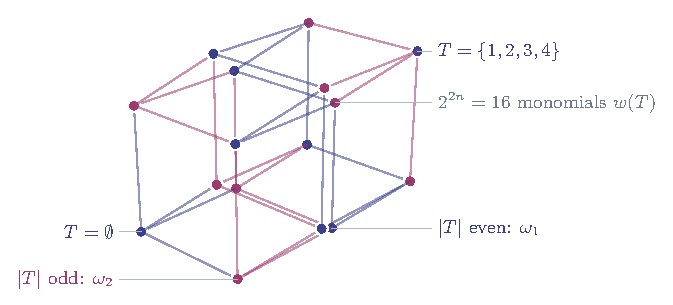
\includegraphics[width=0.78\textwidth]{fig_weilcube}
\caption{The $2^{2n}$ monomials $w(T)$ of \Cref{not:wT}, at $n=2$, drawn as the
vertices of the $4$-cube in a projection that keeps all sixteen distinct. An
edge joins two monomials whose index sets differ in one element. The colouring
is the bipartition by the parity of $\lvert T\rvert$: the eight even vertices
carry $\omega_{1}$ and the eight odd ones carry $\omega_{2}$, so the two
generators of the Weil line are the two halves of the cube and the coefficient
of a monomial depends only on the distance from the empty set.}
\label{fig:weilcoeff}
\end{figure}



\subsection{An elementary proof that the Weil line misses the divisors}

\Cref{prop:notpoly} was deduced from the character computation. In the model
it has a proof with no representation theory in it at all, and the proof
explains the phenomenon in one line: the Weil classes and the powers of the
polarisation are supported on disjoint sets of monomials.

\begin{proposition}[Disjoint supports]\label{prop:disjoint}
In the model of \Cref{thm:model}, every monomial occurring in $\omega_{1}$ or
in $\omega_{2}$ contains exactly one of $x_{j},y_{j}$ for every
$j\in\{1,\dots,2n\}$, and every monomial occurring in $\eta^{k}$ contains
either both or neither, for every $j$ and every $k\ge0$. Consequently
\[
  \HW(A)\cap\QQ\,\eta^{n}=0 ,
\]
and more generally $\HW(A)$ meets the span of the monomials occurring in
powers of $\eta$ in zero.
\end{proposition}

\begin{proof}
The first assertion is \Cref{not:wT}. For the second, $\eta$ is the sum
\eqref{eq:etabasis} of the $2n$ two-forms $x_{j}\wedge y_{j}$, which pairwise
commute and square to zero, so
\[
  \eta^{k}=k!\sum_{\substack{S\subseteq\{1,\dots,2n\}\\|S|=k}}
    \Bigl(\prod_{j\in S}\epsilon_{j}\Bigr)\,
    \bigwedge_{j\in S}\bigl(x_{j}\wedge y_{j}\bigr),
\]
and the monomial indexed by $S$ contains both $x_{j}$ and $y_{j}$ for $j\in S$
and neither for $j\notin S$. A monomial cannot satisfy both patterns for a
given $j$, so the two families of monomials are disjoint, and $2n\ge1$
guarantees that there is at least one index at which to test. Since
$\omega_{1},\omega_{2}$ span $\HW(A)$ by \Cref{thm:explicitgens}(ii), a nonzero
element of $\HW(A)$ has a nonzero coefficient on some $w^{(T)}$, which does not
occur in $\eta^{n}$.
\end{proof}

\begin{remark}\label{rem:twoproofs}
The two proofs of \Cref{prop:notpoly} measure different things.
\Cref{prop:disjoint} is a statement about one model and a choice of basis, and
it is short because the basis was chosen to make the $K$-action diagonal. The
character proof is basis free and applies to every abelian variety of Weil
type, including those not of the form above, and it identifies what the
obstruction is rather than only that there is one. We record both because the
first is checkable by hand and the second is what \Cref{thm:character}
generalises.
\end{remark}

\subsection{All the Hodge classes}

The coordinates also settle how much of the Hodge conjecture for $A$ is at
stake. Recall that the Hodge classes of an abelian variety are the invariants
of the Hodge group,
$\Hdg^{k}(A)=H^{2k}(A,\QQ)^{\Hg(A)}$, where $\Hg(A)\subseteq\SL(V)$ is the
special Mumford--Tate group.

\begin{lemma}[The Hodge group lands in the special unitary group]%
\label{lem:HgSU}
Let $(A,\iota,\eta)$ be of $(K,-1,n)$-Weil type and let $H$ be the
$K$-hermitian form of \Cref{lem:hermform}. Then
\[
  \Hg(A)\subseteq\SU(V,H) .
\]
\end{lemma}

\begin{proof}
By definition $\Hg(A)$ is a $\QQ$-algebraic subgroup of $\SL(V)$ which fixes
every Hodge class in every tensor construction on $V$. It fixes
$\eta\in\bigwedge^{2}V$, hence preserves $Q$; and it commutes with $\iota(K)$,
because each $\iota(\tau)$ is a Hodge class in $V\otimes V^{\vee}$. A
$\QQ$-linear automorphism of $V$ commuting with the $K$-action and preserving
$Q$ preserves $H$, by the formula \eqref{eq:QfromH} expressing $H$ through $Q$
and the $K$-action. Hence $\Hg(A)\subseteq\mathrm{U}(V,H)$. Now
$\HW(A)$ consists of Hodge classes by \Cref{prop:weilline}(ii), so $\Hg(A)$
fixes $\omega_{+}$; and $g\in\mathrm{U}(V,H)$ acts on
$\bigwedge^{2n}V_{+}$ by $\det_{K}(g)$, so $\det_{K}(g)=1$, which is the
definition of $\SU(V,H)$.
\end{proof}

For a very general member of the Weil family the containment of
\Cref{lem:HgSU} is an equality;%
\footnote{Very general means outside a countable union of proper closed analytic subsets of $\cD_{n,n}$, which is the usual meaning in this subject and is the best that can be asked: the locus where the endomorphism algebra jumps is a countable union of such subsets, by \Cref{thm:cdk}, and it is dense in the classical topology.} this is Weil's computation \cite{Weil77}, in
the form given by Moonen and Zarhin \cite{MZ99}. Granting it, the Hodge classes
can be counted exactly.

\begin{theorem}[The full Hodge ring of a general Weil variety]\label{thm:hdgcount}
Let $(A,\iota,\eta)$ be of $(K,-1,n)$-Weil type with
$\Hg(A)=\SU(V,H)$. Then for every $k$ with $0\le k\le 2n$,
\[
  \dim_{\QQ}\Hdg^{k}(A)=
  \begin{cases}
    3, & k=n,\\[2pt]
    1, & k\ne n,
  \end{cases}
  \qquad\text{and}\qquad
  \Hdg^{n}(A)=\QQ\,\eta^{n}\oplus\HW(A).
\]
\end{theorem}

\begin{proof}
Complexify. The group $\SU(V,H)\otimes\CC$ is $\SL(V_{+})\cong\SL_{2n}(\CC)$,
acting on $V_{+}$ tautologically and on $V_{-}$ through the isomorphism
$V_{-}\cong V_{+}^{\vee}$ induced by $H$. By \Cref{prop:grading},
\[
  H^{2k}(A,\CC)=\bigoplus_{r+s=2k}
    \textstyle\bigwedge^{r}V_{+}\otimes\bigwedge^{s}V_{+}^{\vee},
\]
so it suffices to find the invariants in each summand. An invariant is a
weight-zero vector annihilated by every raising operator. In the weight lattice
of $\SL_{2n}$ the weight of $v_{T}\otimes v_{U}^{\vee}$ is
$\mathbf{1}_{T}-\mathbf{1}_{U}$ modulo $(1,1,\dots,1)$; since the entries of
$\mathbf{1}_{T}-\mathbf{1}_{U}$ lie in $\{-1,0,1\}$, the only multiples of
$(1,\dots,1)$ it can equal are $0$ and $\pm(1,\dots,1)$, giving
\[
  T=U \quad(\text{so } r=s),
  \qquad
  (T,U)=\bigl(\{1,\dots,2n\},\emptyset\bigr),
  \qquad
  (T,U)=\bigl(\emptyset,\{1,\dots,2n\}\bigr).
\]
The last two occur only for $(r,s)=(2n,0)$ and $(0,2n)$, each with a
one-dimensional weight-zero space consisting of the invariant lines
$\bigwedge^{2n}V_{+}$ and $\bigwedge^{2n}V_{-}$, which are $\SL$-invariant
because $\SL$ has trivial determinant. For $r=s$ the weight-zero space has
dimension $\binom{2n}{r}$ and its invariant subspace is the line spanned by the
image of the identity under
$\End(\bigwedge^{r}V_{+})\cong\bigwedge^{r}V_{+}\otimes\bigwedge^{r}V_{+}^{\vee}$,
which is one dimensional because $\bigwedge^{r}V_{+}$ is an irreducible
$\SL_{2n}$-module and Schur's lemma applies. The kernel computation confirming
that the invariant space is exactly this line, for all $r,s$ and all $n\le4$,
is item (VII) of \Cref{sec:verification}.

Collecting: for $k\ne n$ the only contribution is $(r,s)=(k,k)$, giving
dimension one, which is $\QQ\eta^{k}$ since $\eta^{k}$ is a nonzero invariant
lying in that summand by \Cref{lem:NSchar}. For $k=n$ there are three
contributions, $(n,n)$, $(2n,0)$ and $(0,2n)$, of total dimension three; the
first is $\QQ\eta^{n}$ and the last two span $\HW(A)\otimes\CC$ by
\Cref{lem:weilchar}. Descending to $\QQ$ preserves dimensions.
\end{proof}

\begin{corollary}[What the Hodge conjecture asks for here]\label{cor:whatisleft}
Let $(A,\iota,\eta)$ be as in \Cref{thm:hdgcount}. The Hodge conjecture holds
for $A$ in every degree if and only if the single class $\omega_{1}$ of
\eqref{eq:omegagens} is algebraic.
\end{corollary}

\begin{proof}
For $k\ne n$ the Hodge classes are the multiples of $\eta^{k}$, which are
algebraic, being powers of a divisor class. For $k=n$ they are spanned by
$\eta^{n}$, $\omega_{1}$ and $\omega_{2}$ by \Cref{thm:hdgcount}. Finally
$\omega_{2}$ is algebraic as soon as $\omega_{1}$ is: by
\Cref{thm:explicitgens}(iv) the plane $\HW(A)$ is a free $K$-module of rank one
generated by $\omega_{1}$, and the action of $\iota(\tau)$ is induced by an
endomorphism of $A$, hence carries algebraic classes to algebraic classes; some
$\tau$ moves $\omega_{1}$ to a class with a nonzero $\omega_{2}$ component, and
the algebraic classes form a $\QQ$-subspace.
\end{proof}

\begin{remark}\label{rem:onlyoneclass}
\Cref{cor:whatisleft} is the reason the Weil line is the standard test case. On
a general abelian variety of Weil type the Hodge conjecture is not a statement
about a large space of classes with some unknown structure; it is a statement
about one explicitly written class with $2^{2n-1}$ integer coefficients. All
three obstruction theorems of this paper are about the difficulty of producing
that one class, and the construction of \Cref{sec:construction} is an attempt
to produce it.
\end{remark}

\begin{figure}[htbp]
\centering
  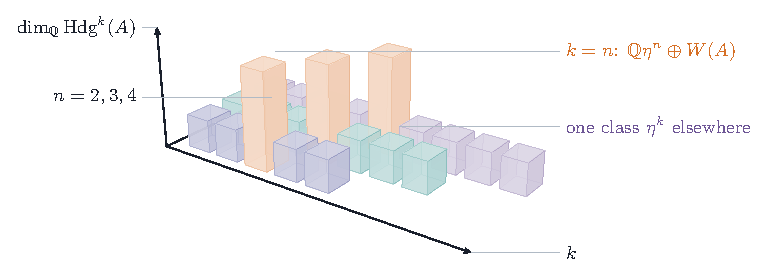
\includegraphics[width=0.9\textwidth]{fig_hodgespike}
\caption{The dimensions of $\Hdg^{k}(A)$ for a general abelian variety of
$(K,-1,n)$-Weil type, drawn as a bar field over the two axes $k$ and $n$, at
$n=2,3,4$, as computed in \Cref{thm:hdgcount}. Every degree carries the one
class $\eta^{k}$; only the middle degree $k=n$ carries anything else, and the
excess there is exactly the two dimensions of the Weil line. The profile is
the same for every $n$, which is why the problem does not get structurally
harder as the dimension grows, only larger.}
\label{fig:hodgespike}
\end{figure}

\section{The character grading and the position of the Weil line}
\label{sec:characters}

This section proves \Cref{thm:character}. The content is a single observation
made precise: the group $\Kx$ acts on $H^{2n}(A,\QQ)$ through the endomorphisms
$\iota(\tau)$, this action grades the cohomology, and the two objects whose
relation is at issue, the Weil line and the power $\eta^{n}$ of the
polarisation, sit at different places in the grading. Once the grading is
written down the obstruction is a two-line argument. What takes work is
writing the grading down correctly, because the natural first guess, that the
Weil line is where $\Kx$ acts through the norm, is wrong, and it is wrong in
exactly the way that makes a construction look as if it should succeed.

\subsection{The grading}

Throughout the section $(A,\iota,\eta)$ is of $(K,-1,n)$-Weil type,
$V=H^{1}(A,\QQ)$, and $V_{\CC}=V_{+}\oplus V_{-}$ is the splitting of
\Cref{not:eigen}.

\begin{proposition}[Character grading]\label{prop:grading}
For every $k\ge0$,
\begin{equation}\label{eq:grading}
  H^{k}(A,\CC)\;=\;\bigoplus_{r+s=k}
    \Bigl(\textstyle\bigwedge^{r}V_{+}\otimes\bigwedge^{s}V_{-}\Bigr),
\end{equation}
and $\iota(\tau)^{*}$ acts on the summand indexed by $(r,s)$ by the scalar
$\tau^{r}\bbar{\tau}^{\,s}$. The summands are the isotypic components for the
action of $\Kx$, and the characters $\tau\mapsto\tau^{r}\bbar{\tau}^{\,s}$ for
distinct pairs $(r,s)$ with $r+s=k$ are pairwise distinct.%
\footnote{Distinctness is a statement about characters of the torus
$\Res_{K/\QQ}\mathbb{G}_{m}$, not about their values at one element. At a
fixed $\tau$ two of the values agree exactly when $\tau/\bbar\tau$ is a root of
unity of order dividing $r-r'$, and for $K=\QQ(\sqrt{-1})$ or
$K=\QQ(\sqrt{-3})$ this happens for the obvious choice $\tau=1+\sqrt{-d}$;
\Cref{sec:lean} records both failures.}
\end{proposition}

\begin{proof}
By \eqref{eq:wedge} we have $H^{k}(A,\CC)=\bigwedge^{k}V_{\CC}$, and the
exterior power of a direct sum decomposes as
$\bigwedge^{k}(V_{+}\oplus V_{-})=\bigoplus_{r+s=k}\bigwedge^{r}V_{+}\otimes\bigwedge^{s}V_{-}$,
which is \eqref{eq:grading}. By \Cref{not:eigen} the operator
$\iota(\tau)^{*}$ acts on $V_{+}$ by $\tau$ and on $V_{-}$ by $\bbar{\tau}$, so
on $\bigwedge^{r}V_{+}\otimes\bigwedge^{s}V_{-}$ it acts by
$\tau^{r}\bbar{\tau}^{\,s}$, as claimed, since it is an algebra map for the
wedge product.

For the last statement, suppose $\tau^{r}\bbar{\tau}^{\,s}=\tau^{r'}\bbar{\tau}^{\,s'}$
for all $\tau\in\Kx$, with $r+s=r'+s'=k$. Dividing, $(\tau/\bbar{\tau})^{r-r'}=1$
for every $\tau\in\Kx$. If $r\ne r'$ this says that the image of the map
$c(\tau)=\tau/\bbar{\tau}$ lies in the group of $(r-r')$-th roots of unity of
$K$, which is finite because $K$ is an imaginary quadratic field and its group
of roots of unity has order $2$, $4$ or $6$. But $c$ has infinite image: two
elements have the same image exactly when their ratio lies in $\QQ^{\times}$,
and the elements $m+\sqrt{-d}$ for $m\in\ZZ$ are pairwise non-proportional over
$\QQ$. Hence $r=r'$ and so $s=s'$.
\end{proof}

\begin{lemma}[The polarisation sits in the middle]\label{lem:NSchar}
Let $(A,\iota,\eta)$ be of $(K,-1,n)$-Weil type. Then
\[
  \iota(\tau)^{*}\eta=\Nm_{K/\QQ}(\tau)\,\eta\qquad\text{for all }\tau\in\Kx,
\]
so $\eta$ lies in the summand $(r,s)=(1,1)$ of \eqref{eq:grading} and
$\eta^{n}$ lies in the summand $(r,s)=(n,n)$, on which $\Kx$ acts by $\Nm^{n}$.
\end{lemma}

\begin{proof}
Let $E$ be the alternating form on $H_{1}(A,\QQ)$ attached to $\eta$. Condition
(iii) of \Cref{def:weiltype} says that the Rosati involution $\dagger$ of
$\eta$ satisfies $\iota(\tau)^{\dagger}=\iota(\bbar{\tau})$, and by the
defining property of the Rosati involution,
\[
  E\bigl(\iota(\tau)x,\,y\bigr)=E\bigl(x,\,\iota(\tau)^{\dagger}y\bigr)
  =E\bigl(x,\,\iota(\bbar{\tau})y\bigr)
  \qquad\text{for all }x,y .
\]
Therefore
\begin{align*}
  \bigl(\iota(\tau)^{*}E\bigr)(x,y)
  &=E\bigl(\iota(\tau)x,\iota(\tau)y\bigr)
   =E\bigl(x,\iota(\bbar{\tau})\iota(\tau)y\bigr)\\
  &=E\bigl(x,\iota(\Nm(\tau))y\bigr)=\Nm(\tau)\,E(x,y),
\end{align*}
using $\bbar{\tau}\tau=\Nm(\tau)\in\QQ$ and the $\QQ$-linearity of $\iota$.
This is the displayed identity. By \Cref{prop:grading} the character $\Nm$ on
$H^{2}$ is $\tau\bbar{\tau}$, which is the summand $(r,s)=(1,1)$; and since
$\iota(\tau)^{*}$ is a ring map, $\iota(\tau)^{*}\eta^{n}=\Nm(\tau)^{n}\eta^{n}$,
placing $\eta^{n}$ in the summand $(n,n)$.
\end{proof}

\begin{lemma}[The Weil line sits at the ends]\label{lem:weilchar}
Let $(A,\iota,\eta)$ be of $(K,-1,n)$-Weil type. Then
\[
  \HW(A)\otimes_{\QQ}\CC
  =\Bigl(\textstyle\bigwedge^{2n}V_{+}\Bigr)\oplus
   \Bigl(\textstyle\bigwedge^{2n}V_{-}\Bigr),
\]
the summands $(r,s)=(2n,0)$ and $(0,2n)$ of \eqref{eq:grading} in degree $2n$,
on which $\Kx$ acts by $\tau\mapsto\tau^{2n}$ and $\tau\mapsto\bbar{\tau}^{\,2n}$.
\end{lemma}

\begin{proof}
This is \Cref{def:weilline} together with \Cref{prop:weilline}(i), which says
that $\HW(A)$ is the $\QQ$-structure on that pair of lines; the characters are
read off from \Cref{prop:grading} with $(r,s)=(2n,0)$ and $(0,2n)$.
\end{proof}

\begin{lemma}[The two characters differ]\label{lem:charsdiffer}
For every $n\ge1$ the characters $\tau\mapsto\tau^{2n}$ and
$\tau\mapsto\Nm_{K/\QQ}(\tau)^{n}=(\tau\bbar{\tau})^{n}$ of $\Kx$ are distinct,
as are $\tau\mapsto\bbar{\tau}^{\,2n}$ and $\Nm^{n}$.
\end{lemma}

\begin{proof}
The two characters agree if and only if $(\tau/\bbar{\tau})^{n}=1$ for every
$\tau\in\Kx$, since $\tau^{2n}=(\tau\bbar{\tau})^{n}$ is equivalent to
$(\tau/\bbar{\tau})^{n}=1$ for $\tau\ne0$.

Consider the map $c\colon\Kx\to\Kx$, $c(\tau)=\tau/\bbar{\tau}$. Two elements
have the same image exactly when their ratio is fixed by conjugation, that is
when it lies in $\QQ^{\times}$. The elements $m+\sqrt{-d}$ for $m\in\ZZ$ are
pairwise non-proportional over $\QQ$, so $c$ takes infinitely many values.

On the other hand $\{\zeta\in K:\zeta^{n}=1\}$ is contained in the group
$\mu(K)$ of roots of unity of $K$, and for an imaginary quadratic field
$\mu(K)$ is finite: it has order $4$ for $d=1$, order $6$ for $d=3$, and order
$2$ otherwise. An infinite set cannot be contained in a finite one, so some
$\tau\in\Kx$ has $(\tau/\bbar{\tau})^{n}\ne1$, and the characters differ. The
second pair is the image of the first under conjugation.
\end{proof}

\begin{remark}[The witness has to be chosen]\label{rem:witness}
The proof just given is non-constructive on purpose, for the following
reason. One is tempted to fix a convenient $\tau$ once and for all, and the
convenient choice $\tau=1+\sqrt{-d}$ fails: for $d=1$ the ratio
$\tau/\bbar{\tau}$ equals $\sqrt{-1}$, a primitive fourth root of unity, so the
two characters do agree at that single $\tau$ whenever $4\mid n$; and for $d=3$
the ratio is $(-1+\sqrt{-3})/2$, a primitive cube root of unity, so they agree
whenever $3\mid n$. The choice $\tau=3+\sqrt{-d}$ fails as well, at $d=3$ with
$6\mid n$. These are not counterexamples to the lemma, which quantifies over
all $\tau$; they are counterexamples to the shortcut. We found them by
formalising the statement, and both are recorded as machine-checked facts in
\Cref{sec:lean}, theorems \texttt{bad\_witness} and
\texttt{bad\_witness\_exceptions}. The choices $\tau=2+\sqrt{-d}$,
$\tau=4+\sqrt{-d}$ and $\tau=3+2\sqrt{-d}$ do work for every $d$ and every
$n\le12$ tested, but the finiteness argument above is what proves the lemma.
\end{remark}

\subsection{The obstruction}

\begin{proof}[Proof of \Cref{thm:character}]
The grading \eqref{eq:grading} and the action on its summands are
\Cref{prop:grading}. The placement of $\HW(A)$ is \Cref{lem:weilchar} and the
placement of $\eta^{n}$ is \Cref{lem:NSchar}. For the last assertion, write
$H^{2n}(A,\QQ)^{\Nm^{n}}$ for the space of $x$ with
$\iota(\tau)^{*}x=\Nm(\tau)^{n}x$ for all $\tau$. After $\otimes\CC$ this is
the isotypic component of the character $\Nm^{n}$, which by
\Cref{prop:grading} is the single summand $(r,s)=(n,n)$. By
\Cref{lem:charsdiffer} the characters $\tau^{2n}$ and $\bbar{\tau}^{\,2n}$ are
different from $\Nm^{n}$, so by \Cref{lem:weilchar} the space
$\HW(A)\otimes\CC$ meets the $(n,n)$ summand in zero. Intersecting with the
rational structure gives $\HW(A)\cap H^{2n}(A,\QQ)^{\Nm^{n}}=0$.
\end{proof}

\begin{corollary}[What an equivariant construction can produce]%
\label{cor:equivariant}
Let $x\in H^{2n}(A,\QQ)$ satisfy $\iota(\tau)^{*}x=\Nm(\tau)^{n}x$ for all
$\tau\in\Kx$. Then the component of $x$ along $\HW(A)$ in any $\Kx$-stable
complement is zero. In particular $x$ is a Weil class only if $x=0$.
\end{corollary}

\begin{proof}
Immediate from \Cref{thm:character}, since the isotypic decomposition is a
direct sum decomposition into $\Kx$-stable subspaces and $x$ lies in a single
summand that meets $\HW(A)$ in zero.
\end{proof}

\Cref{cor:equivariant} is the statement that applies to constructions. A
construction that is natural in the $K$-action produces an eigenclass, and the
computation of which character it produces is usually easy, because it is
determined by how the input transforms. The point of
\Cref{lem:NSchar,lem:charsdiffer} together is that the norm character, which
is the one a $\QQ$-rational construction naturally produces, is the character
already occupied by the polarisation.

\begin{remark}[Which character a construction would need]\label{rem:rightcharacter}
To land on the Weil line a construction must produce an eigenclass for
$\tau\mapsto\tau^{2n}$ or for $\tau\mapsto\bbar{\tau}^{\,2n}$. Neither character
is $\QQ$-valued: $\tau^{2n}\in K$ and is not fixed by $\Gal(K/\QQ)$ unless it
is real. A correspondence defined over $\QQ$ acts on $H^{*}(A,\QQ)$ by a
$\QQ$-linear map that commutes with the $\QQ$-structure, so any eigenvalue
attached to it in this setting is $\Gal(K/\QQ)$-stable as a function of $\tau$,
which forces the norm character or a power of it. The way out of this is not
to make the construction more clever but to break the naturality: one must
produce a class whose $\Kx$-orbit is two-dimensional, spanning the pair
$\tau^{2n}$ and $\bbar{\tau}^{\,2n}$ together, rather than an eigenclass. Both
$\HW(A)$ and its $\QQ$-structure are of that shape, and this is precisely what
makes the Weil line hard to reach: it is the one place in the grading that no
single $\QQ$-rational eigenvalue condition can isolate.
\end{remark}

\begin{remark}[A remark on the failure mode]\label{rem:failuremode}
It is easy to arrive at the opposite conclusion by a plausible sequence of
words. The Weil line is $\bigwedge^{2n}_{K}V$, a rank-one free $K$-module; a
rank-one free $K$-module is two-dimensional over $\QQ$; and $\Kx$ acts on a
two-dimensional $\QQ$-space by matrices of determinant $\Nm(\tau)$. The last
clause is true and irrelevant: the determinant of the action is the norm, but
the action itself is multiplication by $\tau^{2n}$, and a space on which $\Kx$
acts by multiplication by $\tau^{2n}$ is not the same as a space on which it
acts by the scalar $\Nm(\tau)^{n}$. The first is a $K$-line, the second is a
$\QQ$-eigenspace; they agree only when $\tau^{n}=\bbar{\tau}^{\,n}$ for all
$\tau$, which never happens. \Cref{fig:charactergrid} is drawn to make the
distinction visible.
\end{remark}

\begin{figure}[htbp]
\centering
  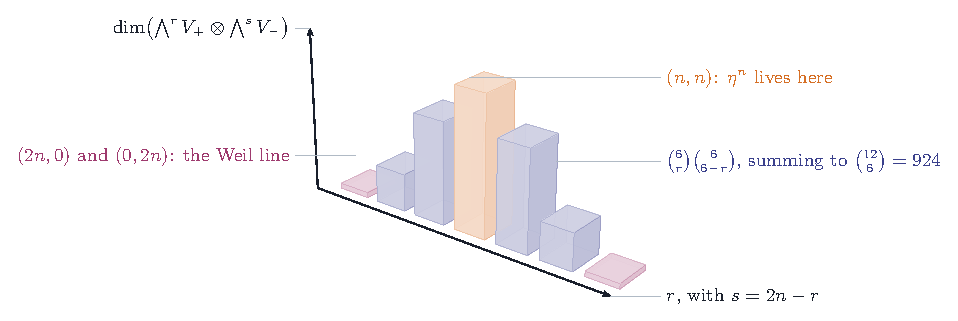
\includegraphics[width=\textwidth]{fig_charactergrid}
\caption{The $\Kx$-grading of $H^{2n}(A,\CC)$ at $n=3$, with each summand
$\bigwedge^{r}V_{+}\otimes\bigwedge^{s}V_{-}$ of \eqref{eq:grading} drawn at
its true dimension $\binom{2n}{r}\binom{2n}{s}$; the seven bars sum to
$\binom{12}{6}=924$. The two extreme cells, $(2n,0)$ and $(0,2n)$, are where
the Weil line sits, and the middle cell $(n,n)$ is where $\eta^{n}$ sits. They
are different cells, which is the whole of \Cref{thm:character}: no
equivariant construction can move a class from the one to the other.}
\label{fig:charactergrid}
\end{figure}

\section{The cohomological Fourier--Mukai transform}\label{sec:fm}

The divisor obstruction rests on one computation: the cohomological
Fourier--Mukai transform sends each power of the polarisation class to a
rational multiple of a power of the polarisation class on the other side, and
to nothing else.%
\footnote{The Todd class of an abelian variety is trivial, since the tangent bundle is trivial, so Grothendieck--Riemann--Roch for a morphism of abelian varieties reduces to the statement that the Chern character commutes with pushforward. That is the one simplification which makes the closed form below a finite computation rather than an estimate, and it is the reason this paper can be precise where the general case would not be.} We prove this in closed form. The computation is universal,
in the sense that it takes place in a cohomology ring whose isomorphism type
is determined by the dimension alone, so a single calculation settles it for
every principally polarised abelian variety at once.

\subsection{Grothendieck--Riemann--Roch on an abelian variety}

\begin{proposition}\label{prop:grr}
Let $A$ be an abelian variety of dimension $g$ and $\cG$ an object of
$D^{b}(\Av)$. Then
\[
  \ch\bigl(\Phi_{\cP}(\cG)\bigr)=\Phi_{\cP}\bigl(\ch(\cG)\bigr),
\]
where the transform on the right is the cohomological one,
$\Phi_{\cP}(x)=p_{*}\bigl(q^{*}x\cdot\ch(\cP)\bigr)$.
\end{proposition}

\begin{proof}
Grothendieck--Riemann--Roch for the proper morphism
$p\colon A\times\Av\to A$ reads
\[
  \ch\bigl(Rp_{*}\cK\bigr)\cdot\td(T_{A})
  =p_{*}\bigl(\ch(\cK)\cdot\td(T_{A\times\Av})\bigr)
\]
for $\cK\in D^{b}(A\times\Av)$. The tangent bundle of an abelian variety is
trivial, so $\td(T_{A})=1$ and $\td(T_{A\times\Av})=1$. Taking
$\cK=Lq^{*}\cG\otimes^{L}\cP$ and using multiplicativity of the Chern
character together with $\ch(Lq^{*}\cG)=q^{*}\ch(\cG)$ gives the statement.
\end{proof}

\subsection{The universal model}

\begin{notation}\label{not:model}
Let $A$ be a principally polarised abelian variety of dimension $g$ with
polarisation class $\theta$, and put $V=H^{1}(A,\QQ)$, a $\QQ$-vector space of
dimension $2g$ carrying the symplectic form attached to $\theta$. Choose a
symplectic basis $e_{1},\dots,e_{2g}$ of $V$, so that
\begin{equation}\label{eq:thetamodel}
  \theta=\sum_{j=1}^{g}e_{j}\wedge e_{g+j}.
\end{equation}
The principal polarisation identifies $\Av$ with $A$ and
$H^{1}(\Av,\QQ)$ with the dual $V^{\vee}$; let $f_{1},\dots,f_{2g}$ be the
basis dual to $e_{1},\dots,e_{2g}$, so that
\begin{equation}\label{eq:thetapmodel}
  \theta'=\sum_{j=1}^{g}f_{j}\wedge f_{g+j}.
\end{equation}
Then $H^{*}(A\times\Av,\QQ)=\bigwedge^{*}(V\oplus V^{\vee})$.
\end{notation}

\begin{lemma}[The Poincar\'e class]\label{lem:poincare}
In the model of \Cref{not:model},
\begin{equation}\label{eq:ell}
  \ell\coloneqq c_{1}(\cP)=\sum_{i=1}^{2g}e_{i}\wedge f_{i}
  \;\in\;V\otimes V^{\vee}\subset\textstyle\bigwedge^{2}(V\oplus V^{\vee}),
\end{equation}
the canonical element of $V\otimes V^{\vee}=\Hom(V,V)$ corresponding to the
identity, and $\ch(\cP)=e^{\ell}$.
\end{lemma}

\begin{proof}
The Poincar\'e bundle is normalised to be trivial on $A\times\{0\}$ and on
$\{0\}\times\Av$, so $c_{1}(\cP)$ has no component in
$\bigwedge^{2}V$ or in $\bigwedge^{2}V^{\vee}$ and lies in the middle summand
$V\otimes V^{\vee}$ of
$\bigwedge^{2}(V\oplus V^{\vee})=\bigwedge^{2}V\oplus(V\otimes V^{\vee})\oplus\bigwedge^{2}V^{\vee}$.
The defining property of $\cP$ is that its restriction to $A\times\{\lambda\}$
is the line bundle $\lambda$; on cohomology this says that the induced map
$H^{1}(\Av,\QQ)\to H^{1}(A,\QQ)^{\vee}$ obtained by contracting $c_{1}(\cP)$ is
the canonical identification. That is exactly the statement that the element
of $\Hom(V,V)$ determined by $c_{1}(\cP)$ is the identity, which is
\eqref{eq:ell}. Since $\cP$ is a line bundle, $\ch(\cP)=e^{c_{1}(\cP)}$.
\end{proof}

\begin{remark}\label{rem:universal}
Every principally polarised abelian variety of dimension $g$ gives the same
data in \Cref{not:model}: a symplectic space of dimension $2g$ over $\QQ$, its
dual, the symplectic form, and the canonical element. The constants computed
below therefore depend only on $g$ and $k$ and not on $A$. This is why a
single computation suffices.
\end{remark}

\subsection{The closed form}

\begin{theorem}[Transform of the polarisation powers]\label{thm:fmtheta}
Let $A$ be a principally polarised abelian variety of dimension $g$. Then for
every $0\le k\le g$,
\begin{equation}\label{eq:fmtheta}
  \Phi_{\cP}\bigl(\theta'^{\,k}\bigr)
  \;=\;(-1)^{\,g(g+1)/2\,+\,k}\,\frac{k!}{(g-k)!}\;\theta^{\,g-k},
\end{equation}
and $\Phi_{\cP}(\theta'^{\,k})=0$ for $k>g$. In particular
$\Phi_{\cP}\bigl(\QQ[\theta']\bigr)=\QQ[\theta]$.
\end{theorem}

\begin{proof}
Work in the model of \Cref{not:model}. By definition
$\Phi_{\cP}(x)=p_{*}(q^{*}x\cdot e^{\ell})$, and $p_{*}$ is the operation of
extracting the coefficient of the top exterior form
$f_{1}\wedge\cdots\wedge f_{2g}$ in the $V^{\vee}$ variables.

The classes $e_{i}\wedge f_{i}$ have even degree, so they commute, and they
have square zero. Hence for every $m$,
\begin{equation}\label{eq:ellpower}
  \frac{\ell^{m}}{m!}
  =\sum_{\substack{S\subseteq\{1,\dots,2g\}\\ |S|=m}}\ \prod_{i\in S}e_{i}\wedge f_{i},
\end{equation}
the product being taken in increasing order of $i$. Likewise, from
\eqref{eq:thetapmodel},
\begin{equation}\label{eq:thetappower}
  \frac{\theta'^{\,k}}{k!}
  =\sum_{\substack{T\subseteq\{1,\dots,g\}\\ |T|=k}}\ \prod_{j\in T}f_{j}\wedge f_{g+j},
  \qquad
  \frac{\theta^{\,g-k}}{(g-k)!}
  =\sum_{\substack{U\subseteq\{1,\dots,g\}\\ |U|=g-k}}\ \prod_{j\in U}e_{j}\wedge e_{g+j}.
\end{equation}

Fix $k$. In the product $\theta'^{\,k}\cdot e^{\ell}$, the terms that survive
$p_{*}$ are those of total degree $2g$ in the $f$ variables. A term of
\eqref{eq:thetappower} indexed by $T$ carries the $2k$ variables
$\{f_{j},f_{g+j}:j\in T\}$, and a term of \eqref{eq:ellpower} indexed by $S$
carries the $|S|$ variables $\{f_{i}:i\in S\}$. For the product to be nonzero
the two index sets must be disjoint, and for the total $f$-degree to be $2g$
we need
\[
  S=\{1,\dots,2g\}\setminus\bigl(T\cup(g+T)\bigr),
  \qquad |S|=2g-2k .
\]
So $S$ is determined by $T$, only the term $\ell^{2g-2k}/(2g-2k)!$ of
$e^{\ell}$ contributes, and the surviving terms are in bijection with the
$k$-subsets $T$ of $\{1,\dots,g\}$. Writing $U=\{1,\dots,g\}\setminus T$ we
have $S=U\cup(g+U)$, so the $V$-part of the term indexed by $T$ is
$\prod_{i\in U\cup(g+U)}e_{i}$, which up to sign is the term of
\eqref{eq:thetappower} indexed by $U$. The bijection $T\leftrightarrow U$ is
exactly the one between the terms of $\theta'^{\,k}/k!$ and those of
$\theta^{\,g-k}/(g-k)!$.

It remains to compute the sign $\sigma$ with which each term contributes, and
to check that it is the same for all $T$. Both are permutation computations in
the ordered word
\[
  \Bigl(\prod_{j\in T}f_{j}f_{g+j}\Bigr)\cdot\Bigl(\prod_{i\in S}e_{i}f_{i}\Bigr)
\]
against the target word
$\bigl(\prod_{j\in U}e_{j}e_{g+j}\bigr)\cdot\bigl(f_{1}\cdots f_{2g}\bigr)$.
Both words use the same multiset of generators, and the permutation relating
them is a product of transpositions whose parity depends only on the
cardinalities $|T|=k$ and $|U|=g-k$, not on which elements $T$ contains,
because relabelling the $g$ symplectic pairs by a permutation $\pi$ of
$\{1,\dots,g\}$ carries the word for $T$ to the word for $\pi(T)$ and
multiplies both words by the same sign. Hence $\sigma=\sigma(g,k)$, and
evaluating it at $T=\{1,\dots,k\}$ gives
\begin{equation}\label{eq:sign}
  \sigma(g,k)=(-1)^{\,g(g+1)/2\,+\,k}.
\end{equation}
Assembling, and accounting for the factorials in \eqref{eq:thetappower},
\[
  \Phi_{\cP}(\theta'^{\,k})
  =k!\cdot\sigma(g,k)\cdot\frac{\theta^{\,g-k}}{(g-k)!},
\]
which is \eqref{eq:fmtheta}. For $k>g$ we have $\theta'^{\,k}=0$ because
$\theta'$ is a symplectic form on a space of dimension $2g$. The last assertion
follows since the constants in \eqref{eq:fmtheta} are nonzero for every
$0\le k\le g$.
\end{proof}

\begin{remark}[On the sign]\label{rem:signcheck}
The identity \eqref{eq:sign} is a finite permutation count for each pair
$(g,k)$. It is verified independently, together with the uniformity of the
sign over all $T$, for every $g\le12$ and every $k$ in
\Cref{app:scripts}; the full expansion of the exterior algebra, which is the
more expensive check and confirms the whole of \eqref{eq:fmtheta} including
the factorials, is carried out there for $g\le4$. For even $g=2n$, which is
the case relevant to Weil type, \eqref{eq:sign} reads
$\sigma(2n,k)=(-1)^{n+k}$.
\end{remark}

\begin{corollary}[Stability of the divisor line]\label{cor:stability}
Let $A$ be a principally polarised abelian variety and let
$x\in H^{*}(\Av,\QQ)$ lie in the subring $\QQ[\theta']$ generated by $\theta'$.
Then $\Phi_{\cP}(x)\in\QQ[\theta]$.
\end{corollary}

\begin{proof}
$\QQ[\theta']$ is spanned by the powers $\theta'^{\,k}$, and
\Cref{thm:fmtheta} sends each to a multiple of a power of $\theta$; extend by
linearity.
\end{proof}

\begin{remark}[Non-principal polarisations]\label{rem:nonprincipal}
If $\theta$ is a polarisation of degree $\delta^{2}$ rather than a principal
one, the isogeny $\phi_{\theta}\colon A\to\Av$ has degree $\delta^{2}$ and one
has $\phi_{\theta}^{*}\theta'=\delta\theta$ for a suitable normalisation of
$\theta'$. The argument of \Cref{thm:fmtheta} goes through with $\theta$
replaced by $\delta^{-1}\phi_{\theta}^{*}\theta'$ and the constants changed by
powers of $\delta$, all of which are nonzero rationals. Since all statements
below concern only membership in $\QQ[\theta]$, and not the values of the
constants, nothing changes. We therefore state the results for principal
polarisations and use them in general.
\end{remark}

\section{The divisor obstruction}\label{sec:divisor}

\subsection{Statement and proof}

\begin{lemma}[Restriction from an ambient projective space]\label{lem:ambient}
Let $Y$ be a smooth projective variety, let $i\colon Y\to\PP^{N-1}$ be a
morphism defined by a linear system, let $h\in H^{2}(\PP^{N-1},\QQ)$ be the
hyperplane class, and let $\cF\in D^{b}(\PP^{N-1})$. Then
\[
  \ch\bigl(Li^{*}\cF\bigr)\in\QQ\bigl[\,i^{*}h\,\bigr]\subset H^{*}(Y,\QQ).
\]
\end{lemma}

\begin{proof}
The Chern character commutes with derived pullback:
$\ch(Li^{*}\cF)=i^{*}\ch(\cF)$. This is standard for a locally free sheaf,
where it follows from naturality of Chern classes, and it extends to
$D^{b}(\PP^{N-1})$ because every object there has a finite resolution by
direct sums of line bundles $\cO(m)$, by Beilinson's theorem, and the Chern
character is additive on distinguished triangles.%
\footnote{Beilinson's theorem gives more than is used here: every object of
$D^{b}(\PP^{N-1})$ is quasi-isomorphic to a finite complex whose terms are
direct sums of $\cO(-m)$ with $0\le m\le N-1$. The proof needs only that
$K_{0}(\PP^{N-1})$ is generated by the classes of line bundles, which already
follows from the Koszul resolutions of the structure sheaves of linear
subspaces; \Cref{rem:otherambient} records which other ambient varieties
behave in the same way.} The cohomology ring of
$\PP^{N-1}$ is $\QQ[h]/(h^{N})$, so $\ch(\cF)$ is a polynomial in $h$ with
rational coefficients, and applying $i^{*}$, a ring homomorphism, gives a
polynomial in $i^{*}h$.
\end{proof}

\begin{lemma}[The hyperplane class of a linear system]\label{lem:hyperclass}
Let $A$ be an abelian variety and $i\colon\Av\to\PP^{N-1}$ a morphism defined
by a linear system $|M|$ with $M\in\Pic(\Av)$. Then
$i^{*}h=c_{1}(M)\in\NS(\Av)\otimes\QQ$.
\end{lemma}

\begin{proof}
A morphism to $\PP^{N-1}$ defined by a linear system $|M|$, or by a subsystem
of it, satisfies $i^{*}\cO(1)\cong M$ by construction, whence
$i^{*}h=c_{1}(i^{*}\cO(1))=c_{1}(M)$.
\end{proof}

\begin{theorem}[\Cref{thm:divisor}]\label{thm:divisor-body}
Let $A$ be a principally polarised complex abelian variety of dimension $g$
with $\NS(\Av)\otimes\QQ=\QQ\cdot\theta'$, let $i\colon\Av\to\PP^{N-1}$ be any
morphism defined by a linear system, and let $\cF$ be any object of
$D^{b}(\PP^{N-1})$. Put $\cE=\Phi_{\cP}(Li^{*}\cF)$. Then
\[
  \ch_{k}(\cE)\in\QQ\cdot\theta^{k}\qquad\text{for every }k\ge0 .
\]
\end{theorem}

\begin{proof}
By \Cref{lem:ambient}, $\ch(Li^{*}\cF)\in\QQ[i^{*}h]$, and by
\Cref{lem:hyperclass}, $i^{*}h=c_{1}(M)$ for the line bundle $M$ defining $i$.
By hypothesis $\NS(\Av)\otimes\QQ=\QQ\theta'$, so $c_{1}(M)=m\theta'$ for some
$m\in\QQ$, and therefore $\ch(Li^{*}\cF)\in\QQ[\theta']$. By
\Cref{cor:stability}, $\Phi_{\cP}$ carries $\QQ[\theta']$ into $\QQ[\theta]$,
so $\ch(\cE)\in\QQ[\theta]$ by \Cref{prop:grr}. Taking the component in
$H^{2k}$ and using that $\QQ[\theta]\cap H^{2k}(A,\QQ)=\QQ\theta^{k}$ gives the
statement.
\end{proof}

\begin{remark}[On the hypothesis on $\NS$]\label{rem:NShyp}
The hypothesis $\NS(\Av)\otimes\QQ=\QQ\theta'$ holds at the very general point
of any positive-dimensional family of abelian varieties of Weil type with
$\End^{0}(A)=\iota(K)$, which is the situation in which the Hodge conjecture
for Weil classes is open; see \Cref{lem:genericNS}. Without it the conclusion
must be stated as $\ch_{k}(\cE)\in D^{2k}(\Av)$ transported to $A$, that is,
$\ch_{k}(\cE)$ lies in the image under $\Phi_{\cP}$ of the divisor subring of
$\Av$. \Cref{thm:character} covers the general case directly and without any
hypothesis on $\NS$, which is one reason to have two proofs.
\end{remark}

\begin{lemma}\label{lem:genericNS}
Let $\mathcal{A}\to S$ be the universal family of abelian varieties of
$(K,-1,n)$-Weil type over the corresponding moduli space, with $n\ge2$. At a
very general point $s\in S$ one has $\End^{0}(A_{s})=\iota(K)$ and
$\NS(A_{s})\otimes\QQ=\QQ\eta_{s}$, of dimension one.
\end{lemma}

\begin{proof}
The locus in $S$ where $\End^{0}$ is strictly larger than $\iota(K)$ is a
countable union of proper closed subvarieties, since each extra endomorphism
imposes a nontrivial algebraic condition on the period point and there are
countably many possible endomorphism algebras; its complement is the very
general locus. At such a point the Hodge group is the full special unitary
group $\mathrm{SU}(V,\psi)$ of the $K$-hermitian form $\psi$ attached to the
polarisation, by Weil's computation of the Hodge group of a general abelian
variety of Weil type. The space $\Hdg^{1}(A_{s})=\NS(A_{s})\otimes\QQ$ is the
space of Hodge-group invariants in $H^{2}(A_{s},\QQ)$. By \Cref{prop:grading}
in degree two,
$H^{2}\otimes\CC=\bigwedge^{2}V_{+}\oplus(V_{+}\otimes V_{-})\oplus\bigwedge^{2}V_{-}$,
and $\mathrm{SU}(V,\psi)$ acts on $V_{+}\otimes V_{-}$ with a one-dimensional
space of invariants, spanned by $\psi$ itself, and on
$\bigwedge^{2}V_{\pm}$ with no invariants for $2n\ge3$, since
$\bigwedge^{2}$ of the standard representation of $\mathrm{SL}_{2n}$ has no
invariant vector unless $2n=2$. Hence the invariants are one-dimensional and
spanned by $\eta_{s}$.
\end{proof}

\subsection{Consequences for Weil classes}

\begin{proof}[Proof of \Cref{cor:neverweil}]
Let $g=2n$ and let $(A,\iota,\eta)$ be of $(K,-1,n)$-Weil type with
$\NS(A)\otimes\QQ=\QQ\eta$. By \Cref{thm:divisor-body},
$\ch_{n}(\cE)\in\QQ\cdot\theta^{n}=\QQ\cdot\eta^{n}\subset D^{2n}(A)$. By
\Cref{prop:notpoly}, $\HW(A)\cap D^{2n}(A)=0$. So if $\ch_{n}(\cE)$ is a Weil
class then it lies in $\HW(A)\cap D^{2n}(A)=0$.
\end{proof}

\begin{proof}[Second proof of \Cref{cor:neverweil}, via characters]
By \Cref{lem:NSchar} the class $\eta^{n}$ is a $\Kx$-eigenclass for the
character $\Nm^{n}$, hence so is every element of $\QQ\eta^{n}$. By
\Cref{thm:divisor-body}, $\ch_{n}(\cE)\in\QQ\eta^{n}$, so $\ch_{n}(\cE)$ is an
eigenclass for $\Nm^{n}$. By \Cref{cor:equivariant} it is a Weil class only if
it vanishes.
\end{proof}

The second proof is longer as written but it is the one that generalises,
because it does not use the hypothesis on $\NS$, only the equivariance. We
record the version that does not mention the ambient space at all.

\begin{theorem}[Equivariance suffices]\label{thm:equivsuffices}
Let $(A,\iota,\eta)$ be of $(K,-1,n)$-Weil type and let $\cE\in D^{b}(A)$ be
an object such that for every $\tau$ in the order
$\iota^{-1}(\End(A))\subset K$ one has
\[
  \iota(\tau)^{*}\ch_{n}(\cE)=\Nm_{K/\QQ}(\tau)^{n}\,\ch_{n}(\cE).
\]
Then $\ch_{n}(\cE)$ is a Weil class only if $\ch_{n}(\cE)=0$.
\end{theorem}

\begin{proof}
The hypothesis says $\ch_{n}(\cE)$ lies in the isotypic component of $\Nm^{n}$
for the action of the order, and this component is the same as the one for the
full group $\Kx$ because the order spans $K$ over $\QQ$ and the action is
$\QQ$-linear. Apply \Cref{cor:equivariant}.
\end{proof}

\begin{remark}[What the two hypotheses cost]\label{rem:twohyp}
\Cref{thm:divisor-body} asks that the object be restricted from an ambient
projective space and imposes a condition on $\NS(\Av)$.
\Cref{thm:equivsuffices} asks only that the resulting class be equivariant
with the norm character. The second hypothesis is weaker and is satisfied
automatically by any construction whose input is $K$-invariant, which is the
case for every secant construction we are aware of, since secant varieties of
a $K$-invariant subvariety are $K$-invariant. The reason to state both is
that the first is checkable by inspection of the construction and the second
requires an equivariance computation.
\end{remark}

\begin{figure}[htbp]
\centering
  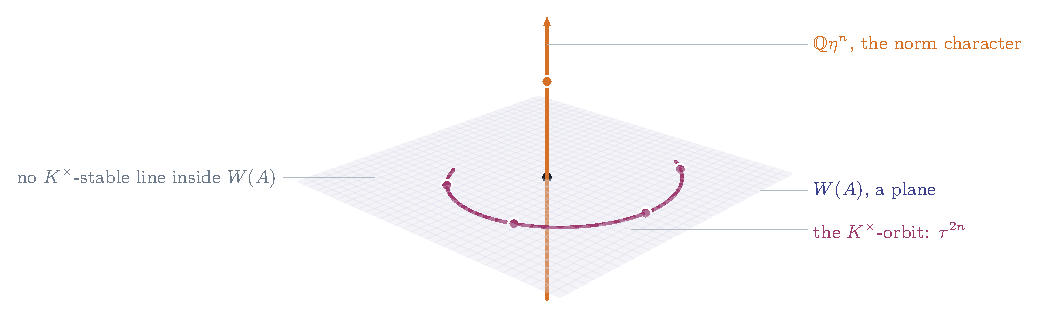
\includegraphics[width=0.96\textwidth]{fig_chernline}
\caption{The linear algebra behind \Cref{thm:divisor}, drawn inside
$H^{2n}(A,\QQ)$. The Weil line $W(A)$ is a plane, free of rank one over $K$
and of rank two over $\QQ$, and $\Kx$ acts on it through $\tau^{2n}$, so the
orbit of any nonzero class is a spiral that spans the plane and lies on no
line in it. The transverse axis carries $\eta^{n}$, on which $\Kx$ acts
through the norm. A construction returning a single eigenclass returns a
line, and by \Cref{prop:orbitplane} no line inside $W(A)$ is stable.}
\label{fig:route}
\end{figure}

\section{The numerical count gives no obstruction}\label{sec:numerology}

An earlier version of part of this material asserted a numerical obstruction
to secant constructions, on the ground that the Euler characteristic which the
dimension count demands lies below the value at which a linear system on an
abelian variety becomes free of base points.%
\footnote{The content of this section was asserted in the opposite direction in the earlier version cited on the title page, where the two thresholds were presented as necessary conditions and used to rule out a range of constructions. They are sufficient and not necessary, and the two counterexamples below are elementary. We have kept the section rather than deleting it, because an error that was believed is worth printing next to its correction.} That assertion is wrong, and
since it is the kind of error that is easy to repeat we set it out and correct
it here. The corrected conclusion is that the numerical count obstructs
nothing; the obstructions in this paper are the two of
\Cref{thm:divisor,thm:character}, and neither uses any count.

\subsection{The count}

\begin{setupenv}[The secant numerology]\label{setup:numerology}
Let $A$ be of $(K,-1,n)$-Weil type, so $\dim A=\dim\Av=2n$. Suppose $\Av$ is
embedded in $\PP^{N-1}$ by a complete linear system $|M|$ with $M$ ample, so
that $N=h^{0}(M)=\chi(M)$. The $n$-th secant variety of a nondegenerate
$2n$-fold has expected dimension
\[
  \dim\Sec^{n}(\Av)=n(2n+1)-1=2n^{2}+n-1,
\]
and a construction that intersects $\Sec^{n}(\Av)$ with $\Av$ in the expected
dimension inside $\PP^{N-1}$ obtains
\[
  \dim\bigl(\Sec^{n}(\Av)\cap\Av\bigr)
  =\bigl(2n^{2}+n-1\bigr)+2n-\bigl(N-1\bigr)
  =2n^{2}+3n-N .
\]
Asking for this to equal $n$, which is what produces a class of the required
codimension, forces
\begin{equation}\label{eq:chirequired}
  N=\chi(M)=2n^{2}+2n .
\end{equation}
\end{setupenv}

\begin{lemma}\label{lem:chicompare}
For every $n\ge2$,
\[
  2n^{2}+2n<2^{2n}<3^{2n},
\]
and the ratio $2^{2n}/(2n^{2}+2n)$ tends to infinity.
\end{lemma}

\begin{proof}
At $n=2$ the left inequality reads $12<16$. For $n\ge2$ the function
$4^{n}/(2n^{2}+2n)$ has ratio of consecutive terms
$4(2n^{2}+2n)/(2(n+1)^{2}+2(n+1))=4n/(n+2)>1$ for $n>2/3$, so the quotient is
increasing from a value exceeding $1$ at $n=2$; both claims follow.
\end{proof}

\subsection{Why this is not an obstruction}

The theorem of Lefschetz says that for $M$ ample on an abelian variety,
$M^{\otimes2}$ is free of base points and $M^{\otimes3}$ is very ample. If
$M=P^{\otimes2}$ with $P$ ample on a variety of dimension $m$, then
$\chi(M)=2^{m}\chi(P)\ge2^{m}$, and similarly $\chi\ge3^{m}$ in the very ample
case. It is tempting to read these as thresholds: no base-point-free system
below $2^{m}$, no very ample system below $3^{m}$. Both readings invert a
sufficient condition into a necessary one, and both are false already for
abelian surfaces.

\begin{proposition}[The thresholds are not necessary]\label{prop:thresholds}
Let $S$ be a general complex abelian surface, so $m=2$.
\begin{enumerate}[label=\textup{(\roman*)},nosep]
\item A polarisation of type $(1,3)$ on $S$ has $\chi=3<4=2^{2}$ and its
  complete linear system is free of base points; the associated morphism
  $S\to\PP^{2}$ is a six-sheeted covering.
\item A polarisation of type $(1,5)$ on $S$ has $\chi=5<9=3^{2}$ and is very
  ample; the image is a Horrocks--Mumford abelian surface of degree $10$ in
  $\PP^{4}$ \textup{\cite{HM73}}.
\end{enumerate}
In particular neither $2^{m}$ nor $3^{m}$ is a lower bound for the Euler
characteristic of a base-point-free, respectively very ample, ample line
bundle on an abelian variety of dimension $m$.
\end{proposition}

\begin{proof}
Both statements are in the classification of $(1,d)$-polarised abelian
surfaces; see Gross and Popescu \cite[\S1.2]{GP98}, where the base locus of
$|L|$ is determined for each $d$: it is empty for $d\ge3$, consists of four
points for $d=2$, and $|L|$ is very ample for $d\ge5$ on a general surface,
the case $d=5$ being the Horrocks--Mumford embedding of \cite{HM73}. The Euler
characteristics are $\chi=d$ by Riemann--Roch on an abelian surface.
\end{proof}

\begin{corollary}\label{cor:nonumerical}
\Cref{setup:numerology} imposes no contradiction. The requirement
$\chi(M)=2n^{2}+2n$ of \eqref{eq:chirequired} is compatible with $M$ being
very ample for all $n$ for which a polarisation of that Euler characteristic
and suitable type exists on a $2n$-dimensional abelian variety; at $n=2$ the
requirement $\chi=12$ on an abelian fourfold is met by polarisations of type
$(1,1,2,6)$ and $(1,1,1,12)$, and nothing in the numerology excludes very
ampleness for either.
\end{corollary}

\begin{remark}[What we retract]\label{rem:retract}
The claim withdrawn here is the assertion that the polarisation required by
\eqref{eq:chirequired} admits no base-point-free linear system. It appeared in
the supplementary material of the earlier version cited on the title page,
together with a table of values of $2n^{2}+2n$, $2^{2n}$ and $3^{2n}$. The
table is arithmetically correct and \Cref{lem:chicompare} reproduces it; the
inference drawn from it is not. We are grateful to have found this before it
propagated, and we note that the obstructions this paper does prove,
\Cref{thm:divisor,thm:character}, are of a different character: they bound
where a class can lie in a decomposition of cohomology, and no choice of
polarisation, ambient space or object affects them.
\end{remark}

\section{The semiregularity target}\label{sec:semireg}

Markman's construction at $n=2$ proceeds by deforming a sheaf across a family
and controlling the obstruction by a semiregularity argument in the sense of
Bloch and of Buchweitz and Flenner \cite{Blo72,BF03}. It is sometimes said
that this route is blocked for $n\ge4$ by a dimension count, the target of the
semiregularity map being too large. We compute the target and show that the
count says nothing of the kind. The section is included because the belief
that the semiregularity route is numerically blocked, combined with the belief
that the secant route is numerically blocked, leaves the impression that the
difficulty at $n\ge4$ is arithmetic. It is not: it is
\Cref{thm:divisor,thm:character}.

\begin{lemma}[Hodge numbers of an abelian variety]\label{lem:hodgenumbers}
For an abelian variety $A$ of dimension $g$ one has
$h^{p,q}(A)=\binom{g}{p}\binom{g}{q}$.
\end{lemma}

\begin{proof}
$H^{p,q}(A)=\bigwedge^{p}H^{1,0}\otimes\bigwedge^{q}H^{0,1}$ by
\eqref{eq:wedge} and the compatibility of the Hodge decomposition with the
exterior algebra structure, and $\dim H^{1,0}=\dim H^{0,1}=g$.
\end{proof}

\begin{proposition}[The semiregularity target]\label{prop:target}
Let $A$ be an abelian variety of dimension $g=2n$. The target of the
semiregularity map, namely $\bigoplus_{q}H^{q+2}(A,\Omega^{q}_{A})$, has
dimension
\[
  \sum_{q\ge0}h^{q,q+2}(A)=\binom{4n}{2n-2}.
\]
\end{proposition}

\begin{proof}
By \Cref{lem:hodgenumbers} with $g=2n$,
\[
  \sum_{q\ge0}h^{q,q+2}
  =\sum_{q\ge0}\binom{2n}{q}\binom{2n}{q+2}
  =\sum_{q\ge0}\binom{2n}{q}\binom{2n}{2n-q-2}
  =\binom{4n}{2n-2},
\]
the last step being the Vandermonde convolution.
\end{proof}

\begin{corollary}[The count does not bind]\label{cor:countnotbind}
The target dimension $\binom{4n}{2n-2}$ takes the values
$28,495,8008,125970,1961256,30421755$ for $n=2,\dots,7$, growing by a factor
exceeding ten at each step. Any source whose dimension grows polynomially in
$n$, for instance the quadratic quantity $\binom{2n}{2}=n(2n-1)$ which takes
the values $6,15,28,45,66,91$ over the same range, is eventually negligible
against it. In particular a comparison of the two dimensions cannot obstruct
the existence of a semiregular sheaf for large $n$; the inequality it produces
points the other way.
\end{corollary}

\begin{remark}[Consistency at $n=2$]\label{rem:markmanconsistent}
At $n=2$ the target is $28$ and the sheaf produced by Markman has
$\dim\Ext^{2}=12$, comfortably inside it, which is consistent with the
construction succeeding there. Nothing in the numbers changes character
between $n=2$ and $n=4$. Whatever prevents the construction from being carried
out for larger $n$, it is not this comparison.
\end{remark}

\begin{remark}[What semiregularity would still need]\label{rem:semiregneed}
We emphasise that \Cref{cor:countnotbind} is not an argument that the
semiregularity route works. It removes one purported obstruction and leaves
the real requirement in place, which is the construction of a sheaf on $A$
whose Chern character has a nonzero component along the Weil line. By
\Cref{thm:character} such a sheaf cannot be $K$-equivariant with the norm
character, so it cannot be produced by any functorial construction from
$K$-invariant data on $\Av$; Markman's sheaf at $n=2$ evades this because it
is not so produced. That is the sense in which the problem for $n\ge3$ is a
problem about breaking equivariance, and not about dimensions.
\end{remark}

\subsection{The annihilator of the Weil line, and objects of rank zero}
\label{ssec:rankzero}

\Cref{rem:semiregneed} says that the remaining requirement is a sheaf whose
Chern character has a component along the Weil line. The most economical way
to arrange that is to make the Chern character lie \emph{entirely} on the
Weil line: to take an object of rank zero, with every $\ch_{k}$ vanishing
except $\ch_{n}$, which is what the construction of \Cref{sec:construction}
does. We show here that this economy is fatal to semiregularity, for a
reason that has nothing to do with how the object is built and everything to
do with where its Chern character sits.%
\footnote{We recall what the map is and what it is for, since the rest of
this subsection turns on it. For a coherent sheaf $\cE$ on a smooth
projective variety $A$ the semiregularity map is defined through the Atiyah
class $\mathrm{at}(\cE)\in\Ext^{1}(\cE,\cE\otimes\Omega^{1}_{A})$: a class
$\xi\in\Ext^{2}(\cE,\cE)$ is sent to the trace of $\xi\cdot\exp(\mathrm{at}(\cE))$,
and the component of that trace in $H^{q}(A,\Omega^{q+2}_{A})=H^{q,q+2}(A)$ is the
$q$-th coordinate of $\sigma_{\cE}(\xi)$. Bloch introduced the map for local
complete intersections \cite{Blo72}, and Buchweitz and Flenner extended it to
arbitrary coherent sheaves and perfect complexes \cite{BF03}. Its use is this. If
$A$ moves in a family $\cA\to S$, the obstruction to extending $\cE$ to first
order along $v\in T_{s}S$ is a class $\mathrm{ob}_{v}(\cE)\in\Ext^{2}(\cE,\cE)$,
and the theorem of Buchweitz and Flenner identifies $\sigma_{\cE}(\mathrm{ob}_{v}(\cE))$
with the derivative of $\ch(\cE)$ in the direction $v$, projected off the
diagonal of the Hodge decomposition. So if $\ch(\cE)$ stays of Hodge type along
$S$ then $\sigma_{\cE}(\mathrm{ob}_{v}(\cE))=0$, and if $\sigma_{\cE}$ is also
injective then $\mathrm{ob}_{v}(\cE)=0$ and $\cE$ deforms. Injectivity is what
converts a statement about the Chern character into a statement about the
sheaf, and it is the one hypothesis in the argument that sees more than
$\ch(\cE)$. Two special cases are all that is needed below: for a line bundle
$L$, $\Ext^{2}(L,L)=H^{2}(\cO_{A})=H^{0,2}(A)$ and $\sigma_{L}$ is multiplication
by $e^{c_{1}(L)}$; and for a direct sum, $\Ext^{2}$ is the sum of the
$\Ext^{2}(\cE_{i},\cE_{j})$ and $\sigma$ acts on each diagonal block by
multiplication by the Chern character of that summand. Both follow at once from
the definition by the trace, and both are what items (XIII) and (XIV) of
\Cref{sec:verification} implement.}

\begin{lemma}[The annihilator of the Weil line in $H^{0,2}$]
\label{lem:annihilator}
Let $A$ be of $(K,-1,n)$-Weil type and let $\omega\in\HW(A)\otimes\CC$ be
any nonzero element of the Weil line. Then the multiplication map
\[
  H^{0,2}(A)\longrightarrow H^{n,n+2}(A),\qquad z\longmapsto z\cdot\omega,
\]
has kernel of dimension exactly $n^{2}$. Its kernel is spanned by the
products $u\wedge v$ with $u\in V_{+}^{0,1}$ and $v\in V_{-}^{0,1}$, and it
is the same subspace for every $\omega$ on the line.
\end{lemma}

\begin{proof}
Write $\omega=a\,\alpha_{+}+b\,\alpha_{-}$ with $\alpha_{\pm}$ generating
$\bigwedge^{2n}V_{\pm}$ and $(a,b)\neq(0,0)$. Since
$H^{0,1}=V_{+}^{0,1}\oplus V_{-}^{0,1}$ with each summand of dimension $n$,
the space $H^{0,2}=\bigwedge^{2}H^{0,1}$ decomposes as
\[
  H^{0,2}
  =\textstyle\bigwedge^{2}V_{+}^{0,1}
  \;\oplus\;\bigl(V_{+}^{0,1}\otimes V_{-}^{0,1}\bigr)
  \;\oplus\;\bigwedge^{2}V_{-}^{0,1},
\]
of dimensions $\binom{n}{2}$, $n^{2}$ and $\binom{n}{2}$.
A mixed product $u\wedge v$ with $u\in V_{+}^{0,1}$, $v\in V_{-}^{0,1}$
satisfies $u\wedge v\wedge\alpha_{+}=0$ because $u$ already occurs among
the $2n$ factors of $\alpha_{+}$, and $u\wedge v\wedge\alpha_{-}=0$ for the
same reason with $v$. So the middle summand lies in the kernel.

Conversely let $z=z_{++}+z_{+-}+z_{--}$ be in the kernel. The product
$z\cdot\omega$ has the component $a\,z_{--}\wedge\alpha_{+}$ in
$\bigwedge^{2}V_{-}^{0,1}\otimes\bigwedge^{2n}V_{+}$ and the component
$b\,z_{++}\wedge\alpha_{-}$ in
$\bigwedge^{2}V_{+}^{0,1}\otimes\bigwedge^{2n}V_{-}$, and these two summands
of $\bigwedge^{2n+2}V_{\CC}$ are independent of each other and of everything
else in $z\cdot\omega$. Each of the maps $z_{--}\mapsto z_{--}\wedge\alpha_{+}$
and $z_{++}\mapsto z_{++}\wedge\alpha_{-}$ is injective, since wedging a
nonzero element of $\bigwedge^{2}V_{-}^{0,1}$ with a basis of $V_{+}$
produces a nonzero element of $\bigwedge^{2n+2}(V_{+}\oplus V_{-})$. Hence
if $a\neq0$ then $z_{--}=0$, and if $b\neq0$ then $z_{++}=0$. When both
$a$ and $b$ are nonzero the kernel is exactly the middle summand. When one
of them vanishes, say $b=0$, the class $\omega=a\,\alpha_{+}$ is not real
and lies in the complexified Weil line; the kernel is then
$V_{+}^{0,1}\otimes V_{-}^{0,1}\oplus\bigwedge^{2}V_{+}^{0,1}$, of dimension
$n^{2}+\binom{n}{2}$. For the rational generators of \Cref{thm:explicitgens},
where $a$ and $b$ are both nonzero, the kernel has dimension exactly $n^{2}$.
\end{proof}

The dimension $n^{2}$ was also computed directly in the exterior algebra,
modulo a prime, for both rational generators of the Weil line at
$n=2,3,4$, and agrees (\Cref{sec:verification}, item (XIV)).

\begin{theorem}[Objects of rank zero are not semiregular]
\label{thm:rankzero}
Let $A$ be of $(K,-1,n)$-Weil type. Let $\cE_{1}$ and $\cE_{2}$ be coherent
sheaves on $A$ such that
\[
  \ch(\cE_{1})-\ch(\cE_{2})=c\,\omega,\qquad c\neq0,\quad \omega\in\HW(A),
\]
and such that $\Ext^{2}(\cE_{1},\cE_{2})=\Ext^{2}(\cE_{2},\cE_{1})=0$. Put
$\cE=\cE_{1}\oplus\cE_{2}$. Then the semiregularity map
\[
  \sigma_{\cE}\colon\ \Ext^{2}(\cE,\cE)\longrightarrow\bigoplus_{q\ge0}H^{q,q+2}(A)
\]
has kernel of dimension at least $n^{2}$. In particular $\cE$ is not
semiregular, for any $n\ge1$.
\end{theorem}

\begin{proof}
The vanishing of the off-diagonal $\Ext^{2}$ groups gives
$\Ext^{2}(\cE,\cE)=\Ext^{2}(\cE_{1},\cE_{1})\oplus\Ext^{2}(\cE_{2},\cE_{2})$,
and each summand contains $H^{2}(\cO_{A})\cdot\id_{\cE_{i}}$ through the
$\cO_{A}$-module structure, the map $z\mapsto z\cdot\id_{\cE_{i}}$ being
injective for $\cE_{i}\neq0$.%
\footnote{The map $H^{2}(\cO_{A})\to\Ext^{2}(\cE,\cE)$, $z\mapsto z\cdot\id_{\cE}$,
is the edge map of the local-to-global spectral sequence, and when $\rk\cE\ne0$ it
is split by the trace up to the factor $\rk\cE$. For a direct sum of line bundles
every summand has rank one, so the map is injective on each block with no
hypothesis, and the element $\xi_{z}$ of the proof, which is $z\cdot\id$ on the
first block and $-z\cdot\id$ on the second, is nonzero for every nonzero $z$.
This is the only place the direct-sum structure is used: it is what allows an
element of $\Ext^{2}$ whose image under $\sigma$ is
$z\cdot(\ch\cE_{1}-\ch\cE_{2})$ rather than $z\cdot(\ch\cE_{1}+\ch\cE_{2})$.
For a single indecomposable sheaf of rank zero the same conclusion holds by the
first sentence of the proof applied to $z\cdot\id_{\cE}$, provided that element
is nonzero, which is the case whenever the restriction of $H^{0,2}(A)$ to the
support of $\cE$ is injective; it fails for a skyscraper sheaf, whose support is
a point, and the theorem is stated for direct sums to keep that hypothesis in
view.} For $z\in H^{2}(\cO_{A})=H^{0,2}(A)$ consider
the element $\xi_{z}=z\cdot\id_{\cE_{1}}-z\cdot\id_{\cE_{2}}$. The
semiregularity map is compatible with direct sums and on the summand
$H^{0,2}\cdot\id_{\cE_{i}}$ it is multiplication by the Chern character of
$\cE_{i}$, so
\[
  \sigma_{\cE}(\xi_{z})=z\cdot\ch(\cE_{1})-z\cdot\ch(\cE_{2})
  =c\,z\cdot\omega .
\]
By \Cref{lem:annihilator} this vanishes for every $z$ in an $n^{2}$-dimensional
subspace of $H^{0,2}$, and the corresponding $\xi_{z}$ are nonzero and
linearly independent. Hence $\dim\ker\sigma_{\cE}\ge n^{2}$.
\end{proof}

\begin{corollary}[The construction of \Cref{sec:construction}]
\label{cor:pteobstructed}
Let $L_{1},\dots,L_{m}$ be line bundles on $A$ with
$\sum_{i}c_{1}(L_{i})=0$ such that the virtual class
$\sum_{i}\bigl([L_{i}]-[L_{i}^{-1}]\bigr)$ has Chern character on the Weil
line and every difference $c_{1}(L_{i})\pm c_{1}(L_{j})$, $i\neq j$, is
nondegenerate of index different from $2$. Then the sheaf
$\bigoplus_{i}(L_{i}\oplus L_{i}^{-1})$ has semiregularity kernel of
dimension at least $n^{2}$. At $n=3$ the explicit object of
\Cref{sec:construction} has kernel of dimension exactly
$15=n^{2}+n(n-1)$, of which the $n^{2}=9$ dimensions on the odd side are
the ones supplied by \Cref{thm:rankzero}; the remaining $n(n-1)=6$ come from
the even side and are specific to the line-bundle structure.
\end{corollary}

\begin{proof}
Take $\cE_{1}=\bigoplus L_{i}$ and $\cE_{2}=\bigoplus L_{i}^{-1}$. The index
hypothesis gives $H^{2}(L_{i}^{\pm1}\otimes L_{j}^{\mp1})=0$ for $i\neq j$
and hence the required $\Ext^{2}$ vanishing, and the Chern character
hypothesis is the one of \Cref{thm:rankzero}. The exact decomposition of
the kernel at $n=3$ into an odd part of dimension $9$ and an even part of
dimension $6$ is a computation, recorded in \Cref{sec:verification}: since
$e^{\lambda}$ and $e^{-\lambda}$ combine into $\cosh\lambda$ and
$\sinh\lambda$, which occupy disjoint degrees, the map splits by parity, and
the odd part is exactly the annihilator of \Cref{lem:annihilator} tensored
with the sign vector.
\end{proof}

\begin{remark}[Every object in the family, and what the theorem says]
\label{rem:familyuniform}
The same computation was run over every configuration
$\lambda_{i}=s_{i}\gamma+c_{i}\ell$ with $\sum s_{i}=\sum c_{i}=0$ in a box
of side $7$ whose virtual Chern character lies on the Weil line: eighteen
distinct configurations, every one with kernel exactly $15$. Adding an
$\eta$-component produced no Weil objects at all in a box of side $3$. The
deficiency is not a defect of the particular six line bundles chosen; it is
the same for every member of the family, and \Cref{thm:rankzero} says why.

What the theorem removes is precisely the economy described at the start of
this subsection. An object realising a Weil class through semiregularity
cannot have its Chern character concentrated on the Weil line. It must carry
a nonzero rank, or nonzero Chern character in other degrees, so that
$z\mapsto z\cdot\ch(\cE)$ is injective on $H^{0,2}$; the degree-two component
of that product is $\rk(\cE)\cdot z$, and rank zero is exactly the case in
which it vanishes. Markman's sheaves have nonzero rank, and this is not incidental to their
success: the class he shows to be deformation-invariant is the normalised
character $\exp(-c_{1}(\cE)/\rk\cE)\ch(\cE)$, which divides by the rank,
and the objects at $n=3$ are reflexive sheaves \cite{Mar25a,Mar25b}. So the fourth ingredient of
\Cref{rem:deformation} is narrowed once more: not a difference of two sheaves
whose classes cancel outside the Weil line, but a single sheaf of positive
rank whose Chern character has a Weil component alongside the rest.
\end{remark}

The hypothesis of \Cref{thm:rankzero} is stated for a direct sum because that
is where the element $\xi_{z}$ is visibly nonzero. The mechanism behind it is
more general, and it reaches the object that \Cref{sec:reduction} uses.

\begin{proposition}[Concentrated Chern characters are never semiregular]
\label{prop:concentrated}
Let $A$ be of $(K,-1,n)$-Weil type and let $E$ be a nonzero perfect complex on
$A$ with $\ch_{k}(E)=0$ for $k\ne n$ and $\ch_{n}(E)=N\omega$ for some
$N\ne0$ and some nonzero $\omega\in\HW(A)$. If the natural map
\begin{equation}\label{eq:idmap}
  H^{2}(\cO_{A})\longrightarrow\Ext^{2}(E,E),\qquad z\longmapsto z\cdot\id_{E},
\end{equation}
is injective, then $\dim\ker\sigma_{E}\ge n^{2}$, so $E$ is not semiregular.
The map \eqref{eq:idmap} is injective whenever $E$ is represented by a virtual
sum of line bundles, in particular at every base point of
\Cref{cor:splitalgebraic}, \Cref{thm:quatweil} and \Cref{thm:everyn}.
\end{proposition}

\begin{proof}
For any perfect complex the semiregularity map satisfies
$\sigma_{E}(z\cdot\id_{E})=z\cdot\ch(E)$, since the trace of
$z\cdot\id_{E}\circ\mathrm{At}(E)^{q}$ is $z$ times the degree-$q$ component
of $\ch(E)$. Hence for $z$ in the annihilator of $\omega$ in $H^{0,2}(A)$,
\[
  \sigma_{E}(z\cdot\id_{E})=N\,z\cdot\omega=0 ,
\]
and that annihilator has dimension exactly $n^{2}$ by
\Cref{lem:annihilator}. If \eqref{eq:idmap} is injective the classes
$z\cdot\id_{E}$ are independent, which gives the bound.

For the last sentence, write $E$ in $K_{0}(A)$ as
$\sum_{i}\varepsilon_{i}[L_{i}]$ with $\varepsilon_{i}=\pm1$ and $L_{i}$ line
bundles, realised as a direct sum of the $L_{i}$ and of shifts of the
remaining ones. The map \eqref{eq:idmap} is then $z\mapsto(z,\dots,z)$ into
$\bigoplus_{i}\Ext^{2}(L_{i},L_{i})=\bigoplus_{i}H^{2}(\cO_{A})$, which is
injective. At a split member $\omega_{1}$ is a polynomial in
$\beta,\widehat\beta,\ell$ by \Cref{thm:splitclosed}(iii), at a quaternionic
member it is a polynomial in divisor classes by \Cref{thm:quatweil}, and at a
product it is one by \Cref{thm:everyn}; in each case the Chern character is a
ring expression in classes of line bundles, so such a representation exists.
\end{proof}

\begin{proposition}[The class forces the size of the object]%
\label{prop:objectsize}
Let $A$ be of $(K,-1,n)$-Weil type, let $\omega$ be a nonzero element of the
Weil line and let $E$ be a perfect complex on $A$ with
\[
  \ch(E)=r+N\omega,\qquad r\in H^{0}(A,\QQ),\ N\ne0,
\]
and no other component. Then
\[
  \chi(E,E)\;=\;(-1)^{n}N^{2}\!\int_{A}\omega^{2},
\]
independently of $r$, and consequently
\[
  \sum_{i}\dim\Ext^{i}(E,E)\;\ge\;N^{2}\Bigl|\int_{A}\omega^{2}\Bigr|\;>\;0 .
\]
\end{proposition}

\begin{proof}
The Todd class of an abelian variety is $1$, so Riemann--Roch for the Ext
algebra reads $\chi(E,E)=\int_{A}\ch(E)^{\vee}\ch(E)$ with
$\ch_{k}^{\vee}=(-1)^{k}\ch_{k}$. Expanding,
\[
  \ch(E)^{\vee}\ch(E)
  = r^{2}+\bigl(1+(-1)^{n}\bigr)rN\omega+(-1)^{n}N^{2}\omega^{2},
\]
and of the three terms only the last has degree $4n$, so only it survives the
integral; the rank enters solely through $r^{2}$, which sits in degree zero.
For the inequality, $\chi(E,E)=\sum_{i}(-1)^{i}\dim\Ext^{i}(E,E)$, so the
total dimension is at least $|\chi(E,E)|$. Finally
$\int_{A}\omega^{2}\ne0$: writing $\omega=\alpha_{+}+\alpha_{-}$ with
$\alpha_{\pm}$ spanning $\bigwedge^{2n}V_{\pm}$, each of $\alpha_{\pm}$ is a
top form on its own eigenspace and squares to zero, so
$\omega^{2}=2\alpha_{+}\alpha_{-}$, which is a nonzero multiple of the
fundamental class. The computation is item (XVIII) of
\Cref{sec:verification}.
\end{proof}

\begin{remark}[The constant, and what it is not]\label{rem:sizeconstant}
The bound is on the whole Ext algebra and is insensitive to the rank, which
is the point: enlarging the rank buys no room. The constant
$|\int\omega^{2}|$ depends on the normalisation of $\omega$; measured against
$\eta$ it picks up factors of $d$ and of the polarisation type, so no
dimension-free growth rate should be read off it. What is intrinsic, and what
the bound uses, is only that the Weil class is not isotropic. Together with
\Cref{prop:concentrated} this says that an object carrying the class is
pinned from two sides at once: its semiregularity map has a kernel of
dimension at least $n^{2}$ unless $H^{2}(\cO_{A})$ acts on it degenerately,
and its Ext algebra has dimension at least $N^{2}|\int\omega^{2}|$ whatever
its rank.
\end{remark}

\begin{remark}[What this does to the semiregularity reduction]
\label{rem:killsreduction}
\Cref{thm:semiregclosure} closes the family under the hypothesis that
$\sigma_{E}$ is injective for the complex $E$ of \Cref{prop:ktheory}, whose
Chern character is $N\omega_{1}$ in degree $n$ and zero elsewhere. That is
exactly the hypothesis of \Cref{prop:concentrated}, so at every base point
this paper constructs the hypothesis of \Cref{thm:semiregclosure} fails for
that complex, and fails by the fixed margin $n^{2}$.

Two things keep this from being a refutation of \Cref{thm:semiregclosure}
itself. The hypothesis is about a chosen perfect complex representing a class
in $K_{0}(A)_{\QQ}$, and distinct representatives of one class have distinct
$\Ext^{2}$ groups, so the theorem is not void; what is ruled out is the
representative the construction supplies. And
\Cref{prop:concentrated} needs \eqref{eq:idmap} to be injective, which is a
genuine hypothesis for an object of rank zero: it fails, for instance, for a
sheaf supported at a point. So a representative escaping
\Cref{prop:concentrated} must receive $H^{2}(\cO_{A})$ non-injectively, which
for a rank-zero object means its support is degenerate. We record the
situation as it stands: of the two reductions of \Cref{sec:reduction}, the
degree bound of \Cref{thm:degreebound} is untouched by anything here, and the
semiregularity reduction of \Cref{thm:semiregclosure} is unavailable for every
object we can presently write down.
\end{remark}

\begin{figure}[t]
\centering
  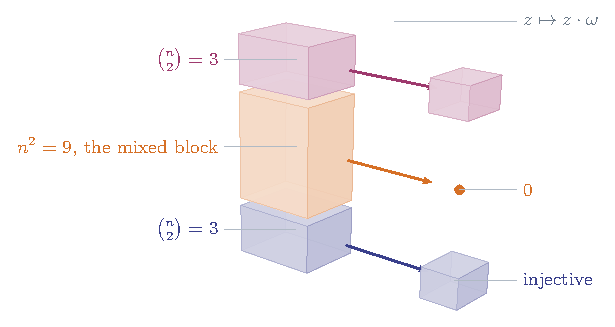
\includegraphics[width=0.94\textwidth]{fig_annihilator}
\caption{The structure behind \Cref{lem:annihilator}, drawn at $n=3$.
$H^{0,2}(A)=\bigwedge^{2}H^{0,1}$ splits into three blocks by how many factors
come from $V_{+}^{0,1}$ and how many from $V_{-}^{0,1}$. The two outer blocks,
of dimension $\binom{n}{2}=3$ each, are carried injectively by multiplication
with the Weil class. The middle block, of dimension $n^{2}=9$ and spanned by
the mixed products, goes to zero, because each such product repeats a factor
of $\alpha_{+}$ and a factor of $\alpha_{-}$. That $n^{2}$ is the deficit in
\Cref{prop:concentrated}.}
\label{fig:annihilator}
\end{figure}


\subsection{The annihilator is the tangent space to the family}
\label{ssec:tangent}

The number $n^{2}$ in \Cref{lem:annihilator} is the dimension of the Weil
family. That is not a coincidence, and this subsection proves it is not: the
polarisation identifies the annihilator with the tangent space to the family,
canonically and in every dimension. Two consequences follow. The first is
that the deficiency of the semiregularity map at an object of rank zero is
not a numerical accident to be repaired by a better choice of object; it is
the family itself, seen inside $H^{0,2}$. The second is that the first-order
Hodge locus of the Weil line is exactly the Weil family, so the directions the
semiregularity map cannot see are precisely the directions along which the
class stays Hodge and would have to be carried.

Write $V_{\pm}$ for the two eigenspaces of $K$ on $H^{1}(A,\CC)$, each of
dimension $2n$, and
\[
  V_{\pm}^{1,0}=V_{\pm}\cap H^{1,0},\qquad
  V_{\pm}^{0,1}=V_{\pm}\cap H^{0,1},
\]
each of dimension $n$ by \Cref{lem:balanced}. Let $E$ denote the
polarisation form on $H^{1}(A,\QQ)$, extended to $H^{1}(A,\CC)$. We use
throughout that $E$ vanishes on $V_{+}\times V_{+}$ and on $V_{-}\times V_{-}$
and pairs $V_{+}$ with $V_{-}$ perfectly, which is condition (iii) of
\Cref{def:weiltype} read on the eigenspaces, and that $E$ vanishes on
$H^{1,0}\times H^{1,0}$ and on $H^{0,1}\times H^{0,1}$, which is the first
Riemann bilinear relation.%
\footnote{The first of these is the computation in the proof of
\Cref{prop:weildomain}: for $x,y\in V_{+}$ one has
$E(\sqrt{-d}\,x,y)=\sqrt{-d}\,E(x,y)$ from the eigenvalue and
$E(\sqrt{-d}\,x,y)=-E(x,\sqrt{-d}\,y)=-\sqrt{-d}\,E(x,y)$ from
\Cref{def:weiltype}(iii), so $E(x,y)=0$; the same on $V_{-}$, and
nondegeneracy of $E$ then forces the pairing between $V_{+}$ and $V_{-}$ to be
perfect. Together the two vanishing statements say that of the four blocks of
$E$ on $(V_{+}^{1,0}\oplus V_{+}^{0,1})\times(V_{-}^{1,0}\oplus V_{-}^{0,1})$
only two are nonzero, namely $V_{+}^{1,0}\times V_{-}^{0,1}$ and
$V_{+}^{0,1}\times V_{-}^{1,0}$, and each of those two is a perfect pairing of
$n$-dimensional spaces. That is the only input to \Cref{thm:anntangent}.}

A first-order deformation of $A$ is a class in $H^{1}(A,T_{A})$, which for an
abelian variety is canonically $\Hom(H^{1,0},H^{0,1})$, since the tangent
bundle is trivial and $H^{1,0}$ is the dual of its space of sections. Such a
$v$ is extended to $H^{1}(A,\CC)$ by zero on $H^{0,1}$ and acts on
$H^{k}(A,\CC)=\bigwedge^{k}H^{1}(A,\CC)$ as the derivation it generates; we
write $v\lrcorner\,\xi$ for that action. A Hodge class $\xi$ of type $(p,p)$
remains of type $(p,p)$ to first order along $v$ exactly when
$v\lrcorner\,\xi=0$. We call $v$ \emph{polarised} when
$E(vx,y)+E(x,vy)=0$ for all $x,y\in H^{1,0}$, which is the condition that the
deformation preserve the polarisation, and the polarised $v$ form a space of
dimension $n(2n+1)=\dim\cA_{2n}$.

\begin{proposition}[The first-order Hodge locus of the Weil line]
\label{prop:firstorder}
Let $A$ be of $(K,-1,n)$-Weil type and let $v$ be a polarised first-order
deformation of $A$. The following are equivalent.
\begin{enumerate}[label=\textup{(\roman*)},nosep]
\item $v\lrcorner\,\omega=0$ for every $\omega$ in the Weil line.
\item $v$ commutes with the action of $K$.
\item $v\bigl(V_{+}^{1,0}\bigr)\subseteq V_{+}^{0,1}$ and
  $v\bigl(V_{-}^{1,0}\bigr)\subseteq V_{-}^{0,1}$.
\end{enumerate}
The space of such $v$ has dimension $n^{2}$, and under
\Cref{prop:weildomain} it is the tangent space at $[A]$ to the Weil family
$\cD_{n,n}$. Already one of the two rational generators of the Weil line cuts
it out.
\end{proposition}

\begin{proof}
The equivalence of (ii) and (iii) is immediate: $K$ acts on $V_{\pm}$ by the
two scalars $\pm\sqrt{-d}$, so commuting with $K$ is preserving $V_{+}$ and
$V_{-}$, and the extension of $v$ kills $H^{0,1}$, so the content is where it
sends $V_{\pm}^{1,0}$.

For (i) and (iii), let $\alpha_{+}$ generate $\bigwedge^{2n}V_{+}$ and write
$\alpha_{+}=e_{1}\wedge\cdots\wedge e_{2n}$ for a basis $e_{1},\dots,e_{2n}$
of $V_{+}$ adapted to $V_{+}=V_{+}^{1,0}\oplus V_{+}^{0,1}$. As a derivation,
\[
  v\lrcorner\,\alpha_{+}
  =\sum_{j=1}^{2n}e_{1}\wedge\cdots\wedge v(e_{j})\wedge\cdots\wedge e_{2n}.
\]
Split $v(e_{j})$ along $H^{1}(A,\CC)=V_{+}\oplus V_{-}$. The $V_{+}$
components contribute
$\operatorname{tr}\bigl(\pi_{+}\circ v|_{V_{+}}\bigr)\,\alpha_{+}$, and that
trace vanishes: the map $\pi_{+}\circ v|_{V_{+}}$ kills $V_{+}^{0,1}$ and
carries $V_{+}^{1,0}$ into $V_{+}^{0,1}$, so in the adapted basis it is
strictly block off-diagonal and has zero diagonal. Writing
$v(e_{j})_{-}=\sum_{k}c_{jk}f_{k}$ for a basis $f_{1},\dots,f_{2n}$ of
$V_{-}$, the $V_{-}$ components contribute
\[
  \sum_{j,k}\pm\,c_{jk}\;
  e_{1}\wedge\cdots\wedge\widehat{e_{j}}\wedge\cdots\wedge e_{2n}\wedge f_{k},
\]
and the $4n^{2}$ monomials appearing here are distinct members of the
standard basis of $\bigwedge^{2n}H^{1}(A,\CC)$, hence linearly independent.
So $v\lrcorner\,\alpha_{+}=0$ if and only if every $c_{jk}$ vanishes, which is
$v(V_{+})\subseteq V_{+}$. The same argument on $\alpha_{-}$ gives
$v\lrcorner\,\alpha_{-}=0$ if and only if $v(V_{-})\subseteq V_{-}$. The Weil
line spans $\bigwedge^{2n}V_{+}\oplus\bigwedge^{2n}V_{-}$ over $\CC$ by
\Cref{prop:weilline}, and each of the two rational generators of
\Cref{thm:explicitgens} has both components nonzero, so a single generator
already forces both conditions. This is (i) if and only if (iii).

For the dimension, let $v$ satisfy (iii) and write $v_{+}$ and $v_{-}$ for
its two blocks. If $x,y$ both lie in $V_{+}^{1,0}$ then $v_{+}x$ and $y$ both
lie in $V_{+}$, so both terms of the polarised condition vanish, and likewise
if both lie in $V_{-}^{1,0}$. For $x\in V_{+}^{1,0}$ and $y\in V_{-}^{1,0}$
the condition reads $E(v_{+}x,y)=-E(x,v_{-}y)$. The left side is determined by
$v_{+}$, and the pairing between $V_{+}^{1,0}$ and $V_{-}^{0,1}$ is perfect,
so this determines $v_{-}y$ for each $y$ and hence determines $v_{-}$ from
$v_{+}$. So the polarised deformations satisfying (iii) are a space of
dimension $\dim\Hom(V_{+}^{1,0},V_{+}^{0,1})=n^{2}$. By
\Cref{prop:weildomain} the family $\cD_{n,n}$ is an open subset of the
Grassmannian of $n$-planes in $V_{+}$, whose tangent space at
$V_{+}^{1,0}$ is $\Hom(V_{+}^{1,0},V_{+}/V_{+}^{1,0})=\Hom(V_{+}^{1,0},V_{+}^{0,1})$,
and the identification just made is that isomorphism.
\end{proof}

\begin{proposition}[Infinitesimal rigidity of divisor classes]%
\label{prop:rigidity}
Keep the notation above and write a class $\delta\in H^{1,1}$ in the four
blocks
\[
  a\ \text{on}\ P\otimes\bbar{P},\quad
  b\ \text{on}\ P'\otimes\bbar{P}',\quad
  c\ \text{on}\ P\otimes\bbar{P}',\quad
  e\ \text{on}\ P'\otimes\bbar{P},
\]
the first two carrying the norm character of $\Kx$ and the last two the
characters $\tau^{2}$ and $\bbar\tau^{\,2}$; reality makes $a$ and $b$
anti-hermitian and ties $e$ to $-\bbar{c}^{\,T}$. Identify the tangent space
to $\cD_{n,n}$ with the $n\times n$ matrices $V$ as in
\Cref{thm:anntangent}. Then contraction with a tangent vector is
\begin{equation}\label{eq:phidelta}
  \Phi_{\delta}(V)
  \;=\;\bigl(\,Va+b^{T}V,\ \ \operatorname{alt}(Vc),\ \
       \operatorname{alt}(-V^{T}e)\,\bigr),
\end{equation}
with values in
$\bbar{P}'\otimes\bbar{P}\oplus\bigwedge^{2}\bbar{P}'\oplus\bigwedge^{2}\bbar{P}
=H^{0,2}$, and $\ker\Phi_{\delta}$ is the tangent space to the locus where
$\delta$ stays of type $(1,1)$. Consequently:
\begin{enumerate}[label=\textup{(\roman*)},nosep]
\item $\Phi_{\delta}=0$ if and only if $\delta$ is a real multiple of $\eta$.
  The rigid classes form a real line, which is the infinitesimal form of the
  statement that $\NS(A)_{\QQ}$ has rank one at the general member.
\item For the norm-character class with block $a$ and $b=c=e=0$,
  \[
    \dim\ker\Phi_{\delta}\;=\;n\,(n-\operatorname{rank}a),
  \]
  so such a class cuts a locus of codimension $n\operatorname{rank}a$, at
  least $n$.
\item A general class has $\ker\Phi_{\delta}=0$: it rigidifies the family to
  a point.
\end{enumerate}
\end{proposition}

\begin{proof}
For \eqref{eq:phidelta}, a polarised deformation commuting with $K$ sends $P$
into $\bbar{P}'$ and $P'$ into $\bbar{P}$, and the symmetry
$E(vx,y)=E(x,vy)$ forces the second matrix to be $-V^{T}$, which is
\Cref{thm:anntangent}. Applying $v$ to the $(1,0)$ slot of each block and
collecting terms in $H^{0,2}$ gives the three displayed components; the sign
in the first comes from $\bbar{P}\wedge\bbar{P}'=-\bbar{P}'\wedge\bbar{P}$.

(i) If $\Phi_{\delta}=0$ then $\operatorname{alt}(Vc)=0$ for every $V$, which
for $n\ge2$ forces $c=0$, and likewise $e=0$. The first component gives
$Va=-b^{T}V$ for every $V$; taking $V$ to run over the matrix units shows
$a$ is a scalar $\lambda$ and $b^{T}=-\lambda$. Anti-hermitian scalars are
the purely imaginary ones, so the solutions form a real line. It contains
$\eta$, whose blocks are $a=i$, $b=-i$, and the two therefore agree.

(ii) With $b=c=e=0$ the condition is $Va=0$, that is, the rows of $V$
annihilate the column space of $a$; the solution space has dimension
$n(n-\operatorname{rank}a)$.

(iii) Immediate from (i) and (ii), and checked on samples.

All three, together with the value $n^{2}$ for the dimension of the tangent
space, are verified over $\QQ(i)$ in exact arithmetic for $n=2,3,4$ in item
(XIX) of \Cref{sec:verification}; at $n=4$ the kernels in (ii) are $12$, $8$,
$4$, $0$ for ranks $1$ to $4$.
\end{proof}

\begin{remark}[Why the count matters here]\label{rem:rigiditywhy}
\Cref{prop:rigidity}(ii) is the reason the divisorial supply of
\Cref{thm:divcriterion} cannot be enlarged by a better choice of class. Any
norm-character class other than a multiple of $\eta$ has
$\operatorname{rank}a\ge1$ and so cuts codimension at least $n$; the locus it
defines is proper, and by (i) no class except the polarisation avoids cutting
at all. So each new class buys a subvariety, never an open set, which is
\Cref{prop:divfails} again with a dimension attached.
\end{remark}

\begin{figure}[htbp]
\centering
  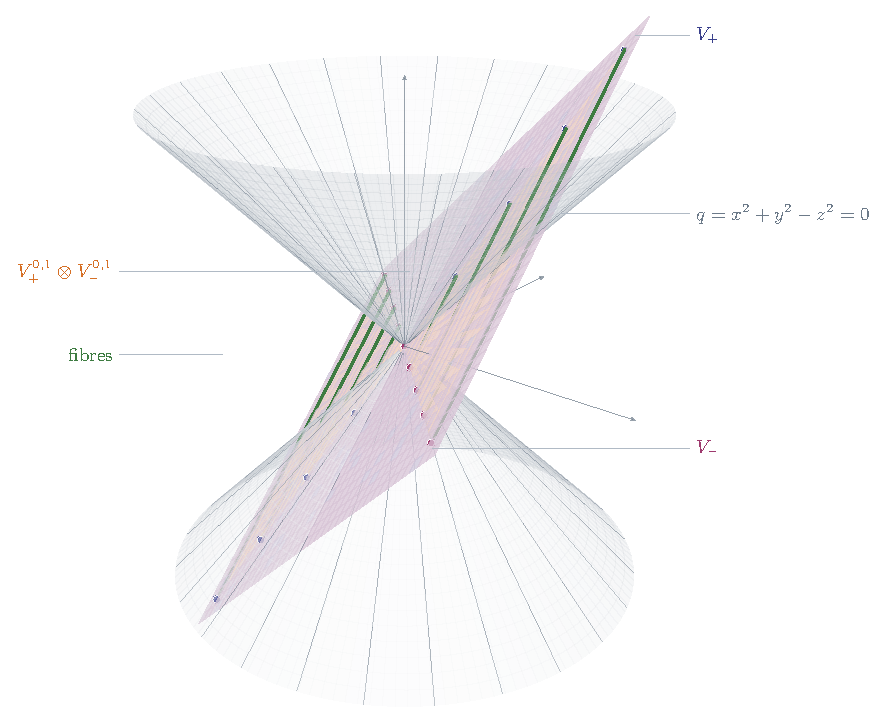
\includegraphics[width=0.46\textwidth]{fig_fibres}
\caption{The geometry behind \Cref{lem:annihilator}, drawn for the real shadow of
the hermitian form. The ruled surface is the null cone of $H$; the two
transverse planes are the conjugate isotropic subspaces $V_{+}$ and $V_{-}$,
which conjugation interchanges, so neither is defined over $\QQ$ and only
their sum is. The segments are the fibres joining a vector of one to its
conjugate in the other, and the strip they sweep is the mixed block
$V_{+}^{0,1}\otimes V_{-}^{0,1}$, of dimension $n^{2}$, which multiplication
by the Weil class sends to zero and which is the deficit in
\Cref{prop:concentrated}. \protect\footnotemark}
\label{fig:fibres}
\end{figure}
\footnotetext{The cone is drawn with its rulings so that it reads as the ruled surface
it is rather than as a shaded volume. The two planes meet only at the origin,
so the fibres are disjoint away from it and the strip they sweep is a cone;
that is why the block is a tensor product and not a direct sum.}

\begin{theorem}[The annihilator is the tangent space]\label{thm:anntangent}
Let $A$ be of $(K,-1,n)$-Weil type and let $\omega$ be a rational generator of
the Weil line. The polarisation induces an isomorphism
\[
  T_{[A]}\cD_{n,n}\;\xrightarrow{\ \sim\ }\;
  \operatorname{Ann}_{H^{0,2}(A)}(\omega),
\]
canonical in the sense that it depends on no choice of basis and on no choice
of $\omega$ on the line. Explicitly, if $p_{1},\dots,p_{n}$ is a basis of
$V_{+}^{1,0}$ and $q_{1},\dots,q_{n}$ the basis of $V_{-}^{0,1}$ dual to it
under $E$, then $\varphi\in\Hom(V_{+}^{1,0},V_{+}^{0,1})$ corresponds to
\[
  \sum_{a=1}^{n}q_{a}\wedge\varphi(p_{a})\;\in\;
  V_{-}^{0,1}\otimes V_{+}^{0,1}\;\subset\;\textstyle\bigwedge^{2}H^{0,1}
  =H^{0,2}(A).
\]
\end{theorem}

\begin{proof}
The form $E$ pairs $V_{+}$ with $V_{-}$ perfectly and vanishes on
$V_{+}^{1,0}\times V_{-}^{1,0}$, the latter because both spaces lie in
$H^{1,0}$. Hence $E$ restricted to $V_{+}^{1,0}\times V_{-}$ kills
$V_{-}^{1,0}$ and descends to a pairing
\[
  V_{+}^{1,0}\times V_{-}^{0,1}\longrightarrow\CC ,
\]
which is perfect, both spaces having dimension $n$ and the total pairing being
nondegenerate. This gives a canonical isomorphism
$\bigl(V_{+}^{1,0}\bigr)^{*}\cong V_{-}^{0,1}$, and therefore
\[
  T_{[A]}\cD_{n,n}
  =\Hom\bigl(V_{+}^{1,0},V_{+}^{0,1}\bigr)
  =\bigl(V_{+}^{1,0}\bigr)^{*}\otimes V_{+}^{0,1}
  \;\cong\;V_{-}^{0,1}\otimes V_{+}^{0,1},
\]
the first equality being the tangent space computation at the end of the proof
of \Cref{prop:firstorder}. Since $H^{0,1}=V_{+}^{0,1}\oplus V_{-}^{0,1}$, the
map $q\otimes u\mapsto q\wedge u$ identifies $V_{-}^{0,1}\otimes V_{+}^{0,1}$
with the middle summand of
$\bigwedge^{2}H^{0,1}$, and that summand is the annihilator by
\Cref{lem:annihilator}. The displayed formula is the composite of these
isomorphisms written in a dual pair of bases, so it is independent of the
basis chosen; and \Cref{lem:annihilator} gives the same subspace for every
$\omega$ on the line, so the isomorphism does not depend on $\omega$ either.
\end{proof}

\begin{figure}[tbp]
\centering
  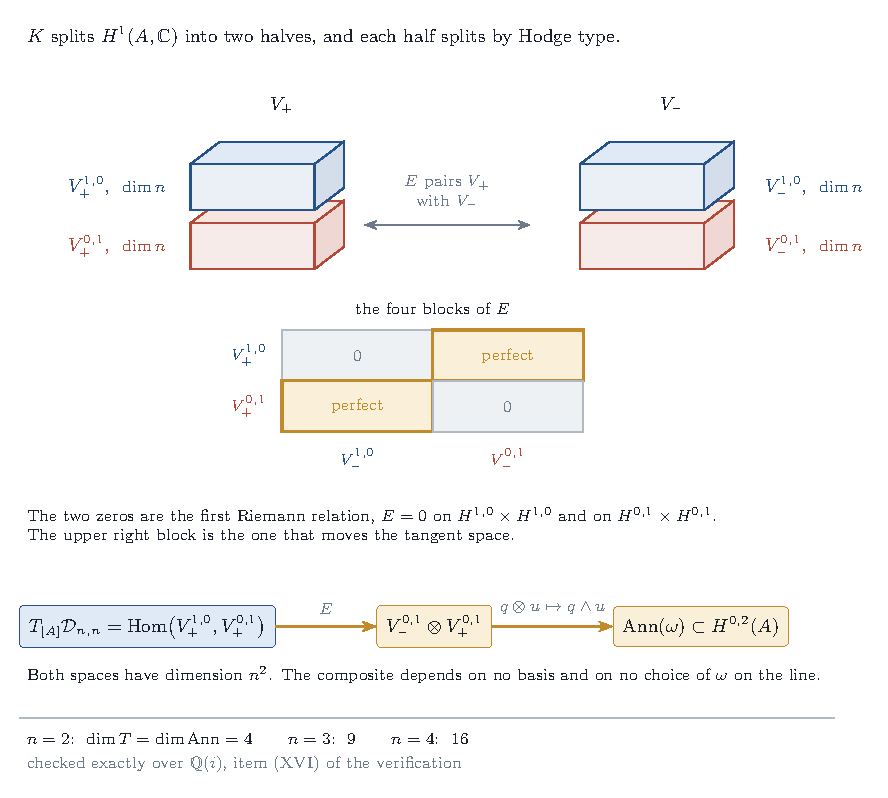
\includegraphics[width=\textwidth]{fig_tangent}
\caption{\Cref{thm:anntangent}. The polarisation has only two nonzero blocks
on $V_{+}\times V_{-}$: it pairs $V_{+}^{1,0}$ with $V_{-}^{0,1}$ and
$V_{+}^{0,1}$ with $V_{-}^{1,0}$, each perfectly, and the other two blocks
vanish by the first Riemann relation. The upper right block turns the tangent
space $\Hom(V_{+}^{1,0},V_{+}^{0,1})$ to the Weil family into
$V_{-}^{0,1}\otimes V_{+}^{0,1}$, which is the middle block of
$\bigwedge^{2}H^{0,1}$ drawn in \Cref{fig:annihilator} and the annihilator of
the Weil line. The two $n^{2}$ dimensional spaces are therefore the same
subspace of $H^{0,2}$, so the directions the semiregularity map cannot see are
the directions of the family along which the class stays Hodge.}
\label{fig:tangent}
\end{figure}


\begin{corollary}[The kernel contains the tangent space to the family]
\label{cor:kernelfamily}
Let $A$ be of $(K,-1,n)$-Weil type and let $E$ be a nonzero perfect complex on
$A$ satisfying the hypotheses of \Cref{prop:concentrated}, that is, with Chern
character concentrated on the Weil line and with \eqref{eq:idmap} injective.
Then $\ker\sigma_{E}$ contains a subspace canonically isomorphic to
$T_{[A]}\cD_{n,n}$, namely the image of the composite
\[
  T_{[A]}\cD_{n,n}\;\cong\;\operatorname{Ann}_{H^{0,2}}(\omega)
  \;\hookrightarrow\;H^{2}(\cO_{A})\;\xrightarrow{\;z\mapsto z\cdot\id_{E}\;}\;
  \Ext^{2}(E,E).
\]
By \Cref{prop:firstorder} that subspace is also the tangent space to the
first-order Hodge locus of the class $\ch_{n}(E)$.
\end{corollary}

\begin{proof}
Immediate from \Cref{thm:anntangent}, \Cref{prop:concentrated} and
\Cref{prop:firstorder}.
\end{proof}

\begin{theorem}[The weakened criterion is unavailable for concentrated
Chern characters]\label{thm:weakfails}
Let $A$ be of $(K,-1,n)$-Weil type and let $E$ be a nonzero perfect complex on
$A$ satisfying the hypotheses of \Cref{prop:concentrated}. Let
\[
  \operatorname{ev}_{E}\colon HH^{2}(A)\longrightarrow\Ext^{2}(E,E)
\]
be the evaluation on $E$ of the natural transformations $\id\to\id[2]$ of
$D^{b}(A)$, as in \cite[Section 11.4]{Mar25b}. Then
\[
  \operatorname{ev}_{E}\bigl(H^{2}(\cO_{A})\bigr)\cap\ker\sigma_{E}
  =\Delta:=\bigl\{\,z\cdot\id_{E}\;:\;z\in\Ann_{H^{0,2}}(\omega)\,\bigr\},
\]
a subspace of dimension $n^{2}$. In particular $\sigma_{E}$ is not injective
on the image of $\operatorname{ev}_{E}$, so $E$ satisfies neither the
hypothesis of \cite[Lemma 11.3]{Mar25b} nor the weakened hypothesis of
\cite[Question 11.4]{Mar25b}.
\end{theorem}

\begin{proof}
The Hochschild cohomology $HH^{*}(A)=\Ext^{*}_{A\times A}(\cO_{\Delta},\cO_{\Delta})$
is the algebra of natural transformations of the identity functor, and the
Hochschild--Kostant--Rosenberg isomorphism \cite{Cal05,BF08} writes
$HH^{2}(A)\cong H^{2}(\cO_{A})\oplus H^{1}(A,T_{A})\oplus H^{0}(A,\bigwedge^{2}T_{A})$,
with no correction from the Todd class because $T_{A}$ is trivial. The first
summand is the image of $H^{2}(\cO_{A})=\Ext^{2}(\cO_{A},\cO_{A})$ under
pullback to $A\times A$, and the natural transformation it defines sends a
complex $F$ to the composite $F=F\otimes\cO_{A}\xrightarrow{\;\id\otimes z\;}
F\otimes\cO_{A}[2]=F[2]$, that is to $z\cdot\id_{F}$; this is the statement
that the action of $HH^{*}(A)$ on $\Ext^{*}(F,F)$ restricts on $H^{*}(\cO_{A})$
to the $\cO_{A}$-module structure.%
\footnote{Concretely: a class $z\in H^{2}(\cO_{A})$ is represented by a
$2$-extension of $\cO_{A}$ by itself, its pullback $\pi_{1}^{*}z$ to
$A\times A$ is a $2$-extension of $\cO_{A\times A}$ by itself, and tensoring
with $\cO_{\Delta}$ gives a $2$-extension of $\cO_{\Delta}$ by itself, which
is the element of $HH^{2}(A)$ in question. The Fourier--Mukai transform with
kernel $\cO_{\Delta}$ is the identity, and the transform with kernel the
extension is the extension of the identity by itself twisted by $z$, so its
value on $F$ is $z\cdot\id_{F}$. Markman uses exactly this identification when
he writes the left vertical arrow of the diagram in the proof of his Lemma
11.3 as HKR followed by contraction with $\ch(E)$: on the summand $H^{2}(\cO_{A})$ contraction is the
cup product $z\mapsto z\cdot\ch(E)$, which is
$\sigma_{E}(z\cdot\id_{E})$ by the computation in the proof of
\Cref{thm:rankzero}.}
Hence $\operatorname{ev}_{E}(z)=z\cdot\id_{E}$ for $z\in H^{2}(\cO_{A})$, and
$\sigma_{E}(z\cdot\id_{E})=z\cdot\ch(E)=N\,z\cdot\omega$ by the proof of
\Cref{prop:concentrated}, which vanishes exactly for
$z\in\Ann_{H^{0,2}}(\omega)$. So
$\operatorname{ev}_{E}(H^{2}(\cO_{A}))\cap\ker\sigma_{E}=\Delta$, and
$\dim\Delta=\dim\Ann_{H^{0,2}}(\omega)=n^{2}$ by \Cref{lem:annihilator} and
the injectivity of \eqref{eq:idmap}. Since $\Delta\ne0$, the restriction of
$\sigma_{E}$ to the image of $\operatorname{ev}_{E}$ has a nonzero kernel.
The hypothesis of \cite[Lemma 11.3]{Mar25b} is that
$\ker\operatorname{ev}_{E}$ equals the kernel of contraction with $\ch(E)$ and
that $\operatorname{ev}_{E}$ is surjective; the second condition would make
$\sigma_{E}$ injective on all of $\Ext^{2}(E,E)$, contradicting
\Cref{prop:concentrated}, and the weakened hypothesis of
\cite[Question 11.4]{Mar25b} is injectivity of $\sigma_{E}$ on the image,
which has just been shown to fail.
\end{proof}

\begin{theorem}[A line bundle summand off the polarisation line obstructs]
\label{thm:linebundle}
Let $A$ be of $(K,-1,n)$-Weil type with $n\ge2$ and let $T=T_{[A]}\cD_{n,n}$.
Let $E$ be a perfect complex on $A$ with a direct summand $L[p]$, $L$ a line
bundle, and suppose that $\ch(E)$ remains of Hodge type to first order along
$\cD_{n,n}$, that is $v\lrcorner\,\ch(E)=0$ for every $v\in T$. If $c_{1}(L)$
is not a real multiple of $\eta$, then there is $v\in T$ with
\[
  \operatorname{ev}_{E}(v)\ne0
  \qquad\text{and}\qquad
  \sigma_{E}\bigl(\operatorname{ev}_{E}(v)\bigr)=0 .
\]
Consequently $E$ is not semiregular, does not satisfy the weakened hypothesis
of \cite[Question 11.4]{Mar25b}, and is obstructed to first order along $v$.
The same holds for a twisted complex, with $c_{1}(L)$ replaced by the twisted
first Chern class of the summand, which is $c_{1}(L)$ shifted by the class
common to all summands.
\end{theorem}

\begin{proof}
The class $c_{1}(L)$ is a real class of type $(1,1)$ and not a real multiple
of $\eta$, so by \Cref{prop:rigidity}(i) the contraction
$\Phi_{c_{1}(L)}\colon T\to H^{0,2}(A)$ is not zero: there is $v\in T$ with
$v\lrcorner\,c_{1}(L)\ne0$. On the summand $H^{1}(A,T_{A})$ of $HH^{2}(A)$ the
evaluation map is contraction with the Atiyah class,
$\operatorname{ev}_{E}(v)=v\lrcorner\,\mathrm{At}(E)$; this is the top row of
the diagram of Buchweitz and Flenner reproduced as \cite[(2.1)]{Mar25b}, and
its identification with the Hochschild evaluation is \cite{BF08}, used by
Markman in the proof of his Lemma 11.3. The Atiyah class of a direct sum is
the direct sum of the Atiyah classes, and that of $L[p]$ is $c_{1}(L)$, so the
component of $\operatorname{ev}_{E}(v)$ in the summand
$\Ext^{2}(L[p],L[p])=H^{0,2}(A)$ of $\Ext^{2}(E,E)$ is
$v\lrcorner\,c_{1}(L)\ne0$. On the other hand the same diagram gives
$\sigma_{E}(\operatorname{ev}_{E}(v))=v\lrcorner\,\ch(E)$, which vanishes by
hypothesis. So $\operatorname{ev}_{E}(v)$ is a nonzero element of
$\ker\sigma_{E}\cap\image\operatorname{ev}_{E}$; this is the failure of both
hypotheses, and $v\lrcorner\,\mathrm{At}(E)\ne0$ is the statement that $E$
does not lift to a first-order deformation of the pair along $v$, as recalled
in \cite[Section 2]{Mar25b}. Twisting by a class $B$ replaces the Atiyah
class of every rank one summand by its shift by $B$ and $\ch(E)$ by the
twisted Chern character, and nothing else in the argument changes.
\end{proof}

\begin{remark}[What this measures, and what it does not settle]
\label{rem:whatmeasures}
The semiregularity criterion converts a statement about the Chern character
into a statement about the object, and it does so by requiring
$\sigma_{E}$ to be injective. \Cref{cor:kernelfamily} says that for an object whose
Chern character is concentrated on the Weil line the requirement fails, and
that the failure is measured by the tangent space to the very family across
which the class is to be transported, in every dimension and with no
hypothesis beyond \eqref{eq:idmap}. That is a statement about the size and the
position of the kernel; by itself it is not a statement that the obstruction
classes are nonzero, and it does not show that the Weil class fails to
deform. For the explicit object of \Cref{prop:explicitobject} the obstruction
classes are computed in \Cref{prop:splitobstruction}: they are nonzero in
every direction of the family normal to the split locus, they lie in
$\ker\sigma_{E}$, and they meet the subspace of \Cref{cor:kernelfamily} only
in zero. The Weil class deforms along the family, by \Cref{prop:firstorder};
that object does not.

Nor does it decide the weaker criterion in the form that matters. Markman
asks, in \cite[Question 11.4]{Mar25b}, whether the semiregularity theorem
survives when $\sigma_{E}$ is required to be injective only on the image of
the evaluation map $\operatorname{ev}_{E}$ rather than on all of
$\Ext^{2}(E,E)$, and records in his Section 12 that an affirmative answer
would carry the method to higher dimensions and to fields of larger degree.
\Cref{thm:weakfails} says that the classes of \Cref{cor:kernelfamily} lie in
that image, so for concentrated Chern characters the weakened hypothesis
fails as well, in every dimension, by the same $n^{2}$ dimensions; and
\Cref{thm:linebundle} says that it fails for every object with a line bundle
summand off the polarisation line, whatever the rank, at every member of the
family, which by \Cref{cor:noline} removes every sum of line bundles from
consideration at once. For the
explicit split object of \Cref{prop:explicitobject} the failure is complete:
\Cref{prop:evaluation} shows that every one of the fifteen dimensions of
$\ker\sigma_{E}$ is the value of $\operatorname{ev}_{E}$ on a Hochschild
class that already preserves $\ch(E)$ to first order. What is not decided,
and what the question is really about, is whether an object of positive rank
can satisfy the weakened hypothesis without satisfying the original one.
Markman's own sheaves are of positive rank and are not of the concentrated
shape, which is \Cref{rem:familyuniform}; he avoids the question for them by
descending to a quotient on which $\sigma_{E}$ is injective on an invariant
subspace containing the image of $\operatorname{ev}_{E}$ \cite[Proposition
11.5]{Mar25b}, and he proposes in his Section 12 a rank one complex on a
principally polarised abelian fourfold, built from $(d+9)/2$ translates of the
theta divisor, as a candidate for the weakened criterion in dimension eight,
with the verification still to be done. \Cref{thm:candidatefails} carries
out that verification and finds that the candidate fails, for every
discriminant, at every isolated double point of its support.

Voisin's account of the present state of the subject \cite{Voi26} makes the
same point qualitatively and for the variational Hodge conjecture at large,
that semiregular objects are hard to construct and too restricted to carry a
general argument. \Cref{cor:kernelfamily} is that observation in quantitative
form for one family of classes: the restriction is exactly $n^{2}$
dimensions, and those dimensions are the family. Totaro's account
\cite{Tot26} is more optimistic about pushing Markman's method further, and
records that it needed the semiregularity theorem for twisted sheaves, which
Pridham supplied \cite{Pri24}.
\end{remark}


\section{The hyperplane obstruction}\label{sec:hyperplane}

We turn to the second attack, induction on the dimension of the variety
through hyperplane sections.%
\footnote{Lefschetz's theorem on hyperplane sections is quoted here in its topological form. The proof by Morse theory, due to Andreotti and Frankel, gives it for any smooth affine variety and is the shortest route; the statement we use is the consequence that $H^{k}(X,\QQ)\to H^{k}(Y,\QQ)$ is an isomorphism for $k<\dim Y$ and injective for $k=\dim Y$.} The ingredients used in such arguments are all
theorems: the Lefschetz hyperplane theorem, hard Lefschetz, the algebraicity
of the Hodge locus \cite{CDK95}, and the properness of relative Hilbert
schemes. The question is whether they compose into an induction, and this
section shows that they do not, for a reason that is elementary and that
applies to every argument of the shape, independently of how the family is
chosen.

Throughout, $X$ is a smooth complex projective variety of dimension $d$,
$j\colon Y\hookrightarrow X$ is a smooth hypersurface in the linear system of
an ample divisor, and $L=c_{1}(\cO_{X}(Y))\in H^{2}(X,\QQ)$.

\subsection{Two classical inputs}

\begin{theorem}[Lefschetz hyperplane theorem]\label{thm:LHT}
The restriction $j^{*}\colon H^{k}(X,\QQ)\to H^{k}(Y,\QQ)$ is an isomorphism
for $k\le d-2$ and is injective for $k=d-1$.
\end{theorem}

\begin{lemma}[Gysin and restriction]\label{lem:gysinrestrict}
For every $k$ and every $x\in H^{k}(X,\QQ)$,
\[
  j_{*}j^{*}x=x\cup L .
\]
Moreover $j_{*}\colon H^{k}(Y,\QQ)\to H^{k+2}(X,\QQ)$ is injective for
$k\ge d$.
\end{lemma}

\begin{proof}
The first identity is the projection formula together with
$j_{*}1=[Y]=L$. For the second, Poincar\'e duality on $X$ and on $Y$
identifies $j_{*}\colon H^{k}(Y)\to H^{k+2}(X)$ with the dual of
\[
  j^{*}\colon H^{2d-k-2}(X)\longrightarrow H^{2(d-1)-k}(Y)=H^{2d-k-2}(Y),
\]
so $j_{*}$ is injective on $H^{k}(Y)$ exactly when this $j^{*}$ is surjective.
By \Cref{thm:LHT} that $j^{*}$ is surjective whenever $2d-k-2\le d-2$, that is
whenever $k\ge d$.
\end{proof}

\subsection{The middle degree}

\begin{proof}[Proof of \Cref{thm:hyperplane}]
Let $d=2p$ and let $\alpha\in H^{2p}(X,\QQ)$ be primitive, which in the middle
degree means $L\alpha=0$, since
$H^{d}_{\mathrm{prim}}(X,\QQ)=\ker\bigl(L\colon H^{d}(X,\QQ)\to H^{d+2}(X,\QQ)\bigr)$.
By \Cref{lem:gysinrestrict},
\[
  j_{*}\bigl(j^{*}\alpha\bigr)=\alpha\cup L=0 .
\]
The class $j^{*}\alpha$ lies in $H^{d}(Y,\QQ)$ and $d\ge d$, so
\Cref{lem:gysinrestrict} says that $j_{*}$ is injective there. Hence
$j^{*}\alpha=0$.
\end{proof}

\begin{corollary}[Blindness in the middle degree]\label{cor:blind}
Let $d=2p$ and let $\alpha,\beta\in H^{2p}(X,\QQ)$ be primitive Hodge classes.
Then $j^{*}\alpha=j^{*}\beta=0$ for every smooth ample hypersurface $Y$. In
particular no property of the restricted classes distinguishes $\alpha$ from
$\beta$, and no statement about Hodge classes on hypersurfaces of $X$, however
strong, carries any information about the primitive middle cohomology of $X$.
\end{corollary}

\begin{remark}[The size of what is lost]\label{rem:sizeofloss}
The primitive middle cohomology is not a small correction term. For a smooth
hypersurface of degree $m$ in $\PP^{d+1}$ its dimension grows like $m^{d+1}$,
and for a general such hypersurface with $d=2p$ the Hodge classes in it are
exactly what the Hodge conjecture is about. \Cref{cor:blind} says that the
whole of it is invisible to hyperplane restriction.
\end{remark}

\subsection{Below the middle degree}

Below the middle degree the restriction map is injective, indeed an
isomorphism, so one can transport the class downwards. The difficulty moves to
the return trip.

\begin{definition}[Lefschetz standard conjecture]\label{def:Bconj}
For a smooth projective variety $X$ of dimension $d$ with ample class $L$,
hard Lefschetz gives isomorphisms
$L^{d-k}\colon H^{k}(X,\QQ)\to H^{2d-k}(X,\QQ)$, and makes $H^{*}(X,\QQ)$
a representation of $\mathfrak{sl}_{2}$ in which $L$ raises the degree by
$2$ and $H$ acts on $H^{k}$ by $k-d$. Let $\Lambda$ denote the unique
endomorphism of degree $-2$ with $[L,\Lambda]=H$. The Lefschetz standard
conjecture $B(X)$ asserts that $\Lambda$ is induced by an algebraic cycle on
$X\times X$; this is equivalent to Kleiman's formulations \cite{Kle68,Kle94}.
\end{definition}

\begin{lemma}[$\Lambda$ undoes $L$ on primitive classes]\label{lem:LambdaL}
Let $\alpha\in H^{k}(X,\QQ)$ be primitive with $k\le d$. Then
$\Lambda L\alpha=(d-k)\,\alpha$.
\end{lemma}

\begin{proof}
This is the $\mathfrak{sl}_{2}$ relation $[L,\Lambda]=H$ of Hodge theory,
where $H$ acts on $H^{k}$ by the scalar $k-d$, together with
$\Lambda\alpha=0$ for $\alpha$ primitive. Explicitly,
$\Lambda L\alpha=L\Lambda\alpha-[L,\Lambda]\alpha=0-(k-d)\alpha
=(d-k)\alpha$.
\end{proof}

\begin{proof}[Proof of \Cref{thm:returntrip}]
Let $2p\le d-2$, so $j^{*}\colon H^{2p}(X,\QQ)\to H^{2p}(Y,\QQ)$ is an
isomorphism by \Cref{thm:LHT}. If $j^{*}\alpha=\cl(W)$ for some
$W\in\CH^{p}(Y)_{\QQ}$, then $j_{*}W\in\CH^{p+1}(X)_{\QQ}$ and
\[
  \cl(j_{*}W)=j_{*}j^{*}\alpha=L\alpha
\]
by \Cref{lem:gysinrestrict}, so $L\alpha$ is algebraic.

For the second statement, suppose $B(X)$ holds and $\alpha$ is primitive of
degree $2p<d$. Then $\Lambda$ is induced by an algebraic correspondence, hence
carries algebraic classes to algebraic classes, and
$\alpha=(d-2p)^{-1}\Lambda(L\alpha)$ by \Cref{lem:LambdaL}, so $\alpha$ is
algebraic. Conversely, suppose that for every smooth projective $X$ and every
Hodge class $\alpha$ the algebraicity of $L\alpha$ implies that of $\alpha$.
Applying this in every degree gives that $\Lambda$ preserves the subspace of
algebraic classes in every degree, which by the standard equivalences for the
Lefschetz conjecture, as set out by Kleiman \cite{Kle68,Kle94}, is $B(X)$.
\end{proof}

\begin{proof}[Proof of \Cref{cor:noinduction}]
Suppose the argument uses only $j^{*}$ and $j_{*}$ to relate classes on $X$ to
classes on smooth ample hypersurfaces $Y\subset X$. If $2p=d$ and $\alpha$ is
primitive, then $j^{*}\alpha=0$ by \Cref{thm:hyperplane}, and $j_{*}$ applied
to any cycle on $Y$ produces a class in the image of $j_{*}$, which by
\Cref{lem:gysinrestrict} and $L\alpha=0$ cannot be $\alpha$ unless $\alpha=0$;
so no conclusion about $\alpha$ is available. Otherwise the best that
$j_{*}j^{*}$ produces is $L\alpha$, and \Cref{thm:returntrip} identifies the
passage from $L\alpha$ to $\alpha$ with $B(X)$.
\end{proof}

\subsection{Diagnosis of a specific inductive scheme}

We record where an induction of this shape breaks in practice,
because the break is usually not where one expects and is easy to miss.

\begin{remark}[The dimension bookkeeping]\label{rem:dimensionbookkeeping}
A common formulation asks the reader to place $X$ in a Lefschetz pencil by
choosing a generic pencil $\{X_{t}\}_{t\in\PP^{1}}$ of hyperplane sections
\emph{of $X$} and then to set $X=X_{t_{0}}$ for some $t_{0}$. The two
requirements are incompatible: the members of a pencil of hyperplane sections
of $X$ have dimension $d-1$, so none of them is $X$. An induction that reads
$\dim X_{t}=d-1<d$ in its inductive step, and $X_{t_{0}}=X$ when it transports
the resulting cycle back, is using both readings of the same symbol.

Resolving the ambiguity in either direction is what
\Cref{thm:hyperplane,thm:returntrip} address. If one insists that $X$ be a
member of the pencil, then the pencil lives in an ambient variety of dimension
$d+1$ and every member has dimension $d$; the inductive parameter does not
decrease and the induction is circular. If instead one keeps
$\dim X_{t}=d-1$, then the class $\alpha$ lives on $X$ and not on the members,
the only available transports are $j^{*}$ and $j_{*}$, and
\Cref{cor:noinduction} applies.
\end{remark}

\begin{remark}[Pointwise existence is not a family]\label{rem:pointwise}
A second gap appears in arguments that produce cycles fibrewise and then
assemble them. Suppose an inductive hypothesis furnishes, for each $t$ in the
base $S$ of a family, a cycle $Z_{t}$ with a prescribed class. It is not
legitimate to conclude that the Hilbert polynomial $t\mapsto P_{Z_{t}}$ is
constructible, or semicontinuous, or takes finitely many values. Those are
theorems about a flat family, and the input here is a bare existence statement
at each point with no coherence between points. Without constructibility there
is no section of a relative Hilbert scheme over a dense open subset, and
therefore nothing for the valuative criterion of properness to extend. The
relative Hilbert scheme is indeed proper over $S$, and that is exactly why the
step looks safe; properness extends a section that exists over a punctured
curve, and supplies no section where none is given.
\end{remark}

\begin{figure}[htbp]
\centering
  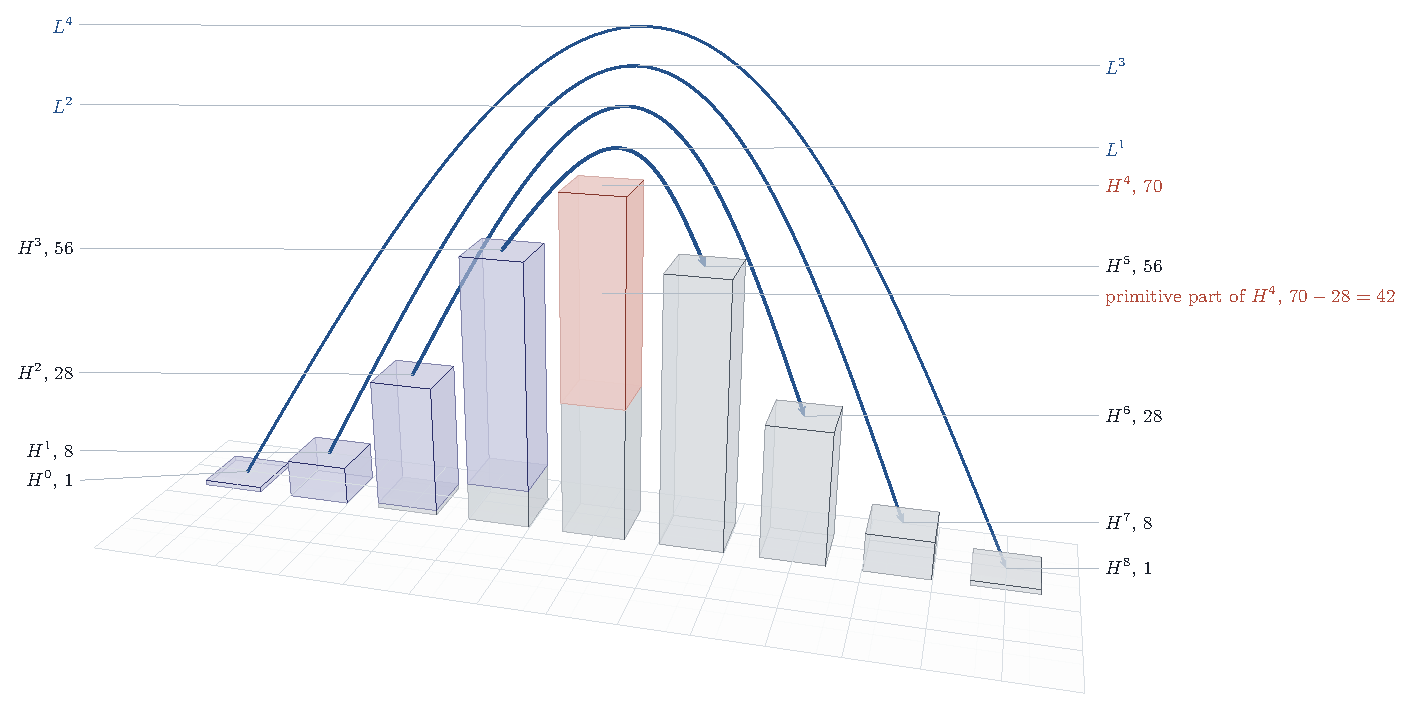
\includegraphics[width=\textwidth]{fig_ladder}
\caption{The Betti numbers $\binom{8}{k}$ of an abelian fourfold, drawn as
prisms, each split into the image of the Lefschetz operator, in slate, and the
primitive part above it, with the hard Lefschetz isomorphisms
$L^{4-k}\colon H^{k}\to H^{8-k}$ drawn as arcs at increasing depth. Below the middle
degree the map $j^{*}$ to a smooth ample hypersurface is injective and the
class descends, but the return trip $j_{*}j^{*}$ multiplies by $L$, so
recovering the class is the Lefschetz standard conjecture. Above the middle
one is reduced to the lower half by an arc. The clay block is the primitive
middle cohomology, of dimension $70-28=42$; it is where the Hodge conjecture
lives, it is annihilated outright by \Cref{thm:hyperplane}, and it is the one
place no arc and no restriction reaches.}
\label{fig:ladder}
\end{figure}

\section{The Kuga--Satake route and where it stops}\label{sec:ks}

\Cref{thm:hyperplane} closes induction on dimension through hyperplane
sections. One classical construction does reach a middle degree Hodge class
without any such induction, and we set it out in full, both because
it shows what a successful route looks like and because its boundary is
numerical and can be located exactly. The construction is Kuga and Satake's
\cite{KS67}, in the form given by Deligne \cite{Del72}. This section builds it,
proves that \Cref{thm:hyperplane} has no bearing on it, and then shows that for
abelian varieties of Weil type it is available precisely when $n=1$, which is
the one case in which the Weil line consists of divisor classes and there is
nothing to prove.

The arithmetic here is checked in \texttt{kugasatake.py}, item (VIII) of
\Cref{sec:verification}.%
\footnote{Kuga and Satake's paper is four pages and constructs the abelian variety; the Hodge-theoretic properties that make it useful, in particular the embedding of \Cref{prop:ksembed}, are Deligne's, and Rapoport's complement to that paper supplies the comparison with the Shimura variety. Satake had already set up the Clifford algebra families in \cite{Sat66}, which is where the Riemann form comes from.}

\subsection{The construction}

\begin{setupenv}[K3 type]\label{setup:k3type}
Let $T$ be a $\QQ$-vector space of dimension $b$ with a nondegenerate
symmetric form $q$, and let $T$ carry a Hodge structure of weight two,
$T_{\CC}=T^{2,0}\oplus T^{1,1}\oplus T^{0,2}$, polarised by $q$, with
\[
  \dim_{\CC}T^{2,0}=1 .
\]
Such a structure is said to be \emph{of K3 type}. Write $T^{2,0}=\CC\sigma$;
the Hodge--Riemann relations give $q(\sigma,\sigma)=0$ and
$q(\sigma,\bbar{\sigma})>0$, so the real plane
$P=\langle\Re\sigma,\Im\sigma\rangle\subset T_{\RR}$ is positive definite and
$q$ has signature $(2,b-2)$ on $T_{\RR}$. Normalise $\sigma$ so that
$e_{1}=\Re\sigma$ and $e_{2}=\Im\sigma$ are orthonormal.
\end{setupenv}

\begin{definition}[Clifford algebra]\label{def:clifford}
$C(T,q)$ is the quotient of the tensor algebra on $T$ by the ideal generated
by $v\otimes v-q(v)$ for $v\in T$. It is $\ZZ/2$-graded, $C=C^{+}\oplus C^{-}$,
by the parity of the word length.
\end{definition}

\begin{lemma}\label{lem:cliffdim}
For an orthogonal basis $f_{1},\dots,f_{b}$ of $T$ the products $f_{S}$ over
subsets $S\subseteq\{1,\dots,b\}$, taken in increasing order, form a basis of
$C(T,q)$. Hence $\dim_{\QQ}C=2^{b}$ and $\dim_{\QQ}C^{\pm}=2^{b-1}$, and
$C^{-}\cdot C^{+}\cdot C^{-}\subseteq C^{+}$.
\end{lemma}

\begin{proof}
The relations $f_{i}^{2}=q(f_{i})$ and $f_{i}f_{j}=-f_{j}f_{i}$ for $i\ne j$,
the latter obtained by expanding $(f_{i}+f_{j})^{2}=q(f_{i})+q(f_{j})$, let one
rewrite any word in the $f_{i}$ as a scalar times an increasing product, so the
$f_{S}$ span; they are independent by the standard filtration argument
comparing $C$ with $\bigwedge^{*}T$. The dimension counts are
$\sum_{k}\binom{b}{k}=2^{b}$ and
$\sum_{k\ \mathrm{even}}\binom{b}{k}=2^{b-1}$. The last statement is the
grading: odd plus even plus odd is even.
\end{proof}

\begin{lemma}[The complex structure]\label{lem:cliffJ}
With $e_{1},e_{2}$ as in \Cref{setup:k3type}, put $J=e_{1}e_{2}\in C^{+}$.
Then $J^{2}=-1$, and left multiplication by $J$ is an $\RR$-linear operator on
$C^{+}\otimes_{\QQ}\RR$ whose square is $-\id$.
\end{lemma}

\begin{proof}
$J^{2}=e_{1}e_{2}e_{1}e_{2}=-e_{1}e_{1}e_{2}e_{2}=-q(e_{1})q(e_{2})=-1$, using
anticommutativity of $e_{1}$ and $e_{2}$ and then $e_{i}^{2}=q(e_{i})=1$.
Left multiplication by an element of $C^{+}$ preserves $C^{+}$, and the square
of left multiplication by $J$ is left multiplication by $J^{2}=-1$.
\end{proof}

\begin{definition}[Kuga--Satake variety]\label{def:ksvariety}
Fix a lattice $C^{+}_{\ZZ}\subset C^{+}$ stable under multiplication. The
complex torus
\[
  \mathrm{KS}(T)=\bigl(C^{+}\otimes_{\QQ}\RR,\,J\bigr)\big/\,C^{+}_{\ZZ}
\]
has dimension $\tfrac12\dim_{\QQ}C^{+}=2^{b-2}$. Satake's construction of a
Riemann form on $C^{+}$ compatible with $J$ \cite{Sat66} makes it an abelian
variety, and by construction
\[
  H^{1}\bigl(\mathrm{KS}(T),\QQ\bigr)=C^{+}(T)
\]
as a Hodge structure of weight one, the Hodge decomposition being the
eigenspace decomposition of left multiplication by $J$.
\end{definition}

\begin{example}\label{ex:ksdims}
For a projective K3 surface, $T$ is the transcendental lattice inside
$H^{2}(X,\QQ)$; taking all of $H^{2}$ with $b=22$ gives
$\dim\mathrm{KS}=2^{20}=1{,}048{,}576$. At the other end, $b=3$ gives
$\dim\mathrm{KS}=2$, an abelian surface; this is the case relevant below.
\end{example}

\subsection{What the construction transports}

\begin{proposition}[The embedding]\label{prop:ksembed}
Fix $v_{0}\in T$ with $q(v_{0})\ne0$. The map
\[
  \Psi\colon T\longrightarrow\End_{\QQ}\bigl(C^{+}\bigr),
  \qquad
  \Psi(v)(x)=v\,x\,v_{0},
\]
is injective and is a morphism of Hodge structures
$T(1)\to\End\bigl(H^{1}(\mathrm{KS}(T),\QQ)\bigr)$, both sides having weight
zero. Consequently a Hodge class in $T$, that is a rational class of type
$(1,1)$, is carried to a Hodge class of type $(0,0)$ in
$\End(H^{1}(\mathrm{KS}(T),\QQ))$, that is to an element of
$\End^{0}(\mathrm{KS}(T))$.
\end{proposition}

\begin{proof}
The map lands in $\End(C^{+})$ by the last part of \Cref{lem:cliffdim}, since
$v,v_{0}\in T\subset C^{-}$. It is injective because
$\Psi(v)(v_{0}^{-1})=v$, where $v_{0}^{-1}=v_{0}/q(v_{0})$. That it respects
the Hodge structures is Deligne's computation \cite[\S4]{Del72}: the
Hodge structure on $\End(C^{+})$ is induced by $J$ acting on both sides, and
$\Psi$ intertwines the weight-two structure on $T$, twisted once, with it.
The last sentence is the definition of a morphism of Hodge structures together
with the theorem of Lefschetz on $(1,1)$ classes in the form that says a Hodge
class of type $(0,0)$ in $\End(H^{1}(B,\QQ))$ of an abelian variety $B$ is an
element of $\End^{0}(B)$.
\end{proof}

\begin{remark}[What is and is not known about the transport]%
\label{rem:kstransport}
The graph of an element of $\End^{0}(\mathrm{KS}(T))$ is an algebraic cycle on
$\mathrm{KS}(T)\times\mathrm{KS}(T)$, so the image of a Hodge class under
$\Psi$ is algebraic. Carrying that conclusion back to the variety $X$ from
which $T$ came requires the correspondence $\Psi$ itself to be induced by an
algebraic cycle on $X\times\mathrm{KS}(T)\times\mathrm{KS}(T)$, and that is
what is not known in general. What is known is that $\Psi$ is absolute Hodge,
by Deligne's theorem for abelian varieties together with the analysis of the
Kuga--Satake correspondence, and that it is motivated in Andr\'e's sense
\cite{And96}; van Geemen \cite{vG00} surveys the cases where algebraicity has
been established. So the Kuga--Satake route converts the Hodge conjecture for
$T$ into the algebraicity of one specific correspondence, which is progress of
a definite kind and is not a proof.
\end{remark}

\subsection{The hyperplane obstruction does not apply}

\begin{proposition}\label{prop:ksnotrestriction}
\Cref{thm:hyperplane,thm:returntrip} do not constrain the Kuga--Satake route.
\end{proposition}

\begin{proof}
Both theorems are statements about the pair of maps $j^{*}$ and $j_{*}$
attached to the inclusion $j\colon Y\hookrightarrow X$ of a smooth member of an
ample linear system, and both proofs use two properties of that pair which no
other correspondence has: the Lefschetz hyperplane theorem, which makes
$j^{*}$ an isomorphism below the middle degree and hence forces the
vanishing of \Cref{lem:gysinrestrict} in the primitive middle degree; and the
identity $j_{*}j^{*}=\,\cdot\,\eta$, which is what makes the return trip
multiply by the polarisation rather than recover the class. The Kuga--Satake
correspondence is a cycle class on a triple product of varieties of unrelated
dimensions, $\dim\mathrm{KS}(T)=2^{b-2}$ against $\dim X$, and it satisfies
neither property; in particular the composite of $\Psi$ with its transpose is
multiplication by $q(v_{0})$ on $T$ and not by a power of any polarisation of
$X$. So neither hypothesis of \Cref{thm:hyperplane} is met.
\end{proof}

This is the content already asserted in \Cref{rem:ksscope}. The point of
isolating it is that it identifies what an escape from \Cref{thm:hyperplane}
must look like: a correspondence whose transpose composite is not the
Lefschetz operator. \Cref{sec:escape} makes the analogous identification for
\Cref{thm:divisor,thm:character}.

\subsection{Where the route stops for Weil type}

The limitation of the Kuga--Satake construction is the hypothesis
$\dim T^{2,0}=1$, and for abelian varieties of Weil type the possible values of
$\dim T^{2,0}$ can be listed completely.

\begin{proposition}[The pieces of \texorpdfstring{$H^{2}$}{H2}]\label{prop:h2pieces}
Let $(A,\iota,\eta)$ be of $(K,-1,n)$-Weil type. In the character grading of
\Cref{prop:grading},
\begin{equation}\label{eq:h2split}
  H^{2}(A,\CC)
  =\textstyle\bigwedge^{2}V_{+}\;\oplus\;\bigl(V_{+}\otimes V_{-}\bigr)
   \;\oplus\;\bigwedge^{2}V_{-},
\end{equation}
the middle summand is the isotypic component of the norm character and is
defined over $\QQ$, and the outer two are interchanged by conjugation so their
sum is defined over $\QQ$. The Hodge numbers are
\[
  \bigl(h^{2,0},h^{1,1},h^{0,2}\bigr)=
  \begin{cases}
    \bigl(\tbinom{n}{2},\,n^{2},\,\tbinom{n}{2}\bigr)
      & \text{on }\bigwedge^{2}V_{\pm},\\[4pt]
    \bigl(n^{2},\,2n^{2},\,n^{2}\bigr)
      & \text{on }V_{+}\otimes V_{-},
  \end{cases}
\]
and the total is $2\tbinom{2n}{2}+4n^{2}=\tbinom{4n}{2}=\dim H^{2}(A,\QQ)$.
\end{proposition}

\begin{proof}
The splitting is \eqref{eq:grading} at $k=2$. The characters are
$\tau^{2}$, $\tau\bbar{\tau}=\Nm(\tau)$ and $\bbar{\tau}^{2}$, so the middle
summand is the norm-isotypic component, and it is self-conjugate, hence defined
over $\QQ$; the outer two are exchanged. For the Hodge numbers use
\eqref{eq:bisplit} and \Cref{lem:balanced}: $V_{\pm}^{1,0}$ and
$V_{\pm}^{0,1}$ have dimension $n$ each, so
$(\bigwedge^{2}V_{+})^{2,0}=\bigwedge^{2}V^{1,0}_{+}$ has dimension
$\binom{n}{2}$ and $(\bigwedge^{2}V_{+})^{1,1}=V^{1,0}_{+}\otimes V^{0,1}_{+}$
has dimension $n^{2}$, while
$(V_{+}\otimes V_{-})^{2,0}=V^{1,0}_{+}\otimes V^{1,0}_{-}$ has dimension
$n^{2}$ and the $(1,1)$ part has dimension $2n^{2}$. The total is
$2(2\binom{n}{2}+n^{2})+4n^{2}=2(2n^{2}-n)+4n^{2}=8n^{2}-2n=\binom{4n}{2}$.
\end{proof}

\begin{proposition}[No K3-type piece beyond \texorpdfstring{$n=1$}{n=1}]%
\label{prop:normpart}
Let $(A,\iota,\eta)$ be of $(K,-1,n)$-Weil type with $\Hg(A)=\SU(V,H)$. Then
$H^{2}(A,\QQ)$ decomposes into exactly three rational sub-Hodge structures that
cannot be decomposed further, namely
\[
  \QQ\,\eta,
  \qquad
  \bigl(V_{+}\otimes V_{-}\bigr)_{\QQ}\ominus\QQ\eta,
  \qquad
  \Bigl(\textstyle\bigwedge^{2}V_{+}\oplus\bigwedge^{2}V_{-}\Bigr)_{\QQ},
\]
with $h^{2,0}$ equal to $0$, $n^{2}$ and $n(n-1)$ respectively. Consequently
$H^{2}(A,\QQ)$ contains a rational sub-Hodge structure of K3 type if and only
if $n=1$.
\end{proposition}

\begin{proof}
A rational sub-Hodge structure $W\subseteq H^{2}(A,\QQ)$ is stable under
$\Hg(A)$: the orthogonal projector onto $W$ for the polarisation is a Hodge
class in $\End(H^{2})$, hence is fixed by $\Hg(A)$, hence $W$ is a
$\Hg(A)$-submodule. Conversely a $\Hg(A)$-submodule is a sub-Hodge structure,
because the Hodge decomposition is the eigenspace decomposition of an element
of $\Hg(A)(\RR)$. So the rational sub-Hodge structures are the
$\QQ$-subrepresentations of $\SU(V,H)$.

After complexification $\SU(V,H)$ becomes $\SL(V_{+})$, acting on $V_{+}$
tautologically and on $V_{-}\cong V_{+}^{\vee}$ dually. In \eqref{eq:h2split}
the outer summands $\bigwedge^{2}V_{+}$ and $\bigwedge^{2}V_{-}$ are
irreducible, being fundamental representations, and the middle summand is
$V_{+}\otimes V_{+}^{\vee}=\End(V_{+})=\mathfrak{sl}(V_{+})\oplus\CC$, the sum
of the adjoint representation and the trivial one. This gives four complex
irreducible pieces; conjugation fixes the two coming from the middle and
exchanges the outer two, so over $\QQ$ they group into the three listed
structures, and no further splitting is possible.

The trivial summand is spanned by $\eta$ by \Cref{lem:NSchar}, and has
$h^{2,0}=0$ since $\eta$ is of type $(1,1)$. The adjoint summand has
$h^{2,0}=n^{2}$, since removing the one-dimensional trivial piece from
$V_{+}\otimes V_{-}$ removes a $(1,1)$ class only. The outer structure has
$h^{2,0}=2\binom{n}{2}=n(n-1)$ by \Cref{prop:h2pieces}.

For a sum of these to have $h^{2,0}=1$ we need one of $n^{2}$, $n(n-1)$,
$n^{2}+n(n-1)=2n^{2}-n$ to equal $1$, using $h^{2,0}(\QQ\eta)=0$. The equation
$n(n-1)=1$ has no positive integer solution, and each of $n^{2}=1$ and
$2n^{2}-n=1$ gives $n=1$. At $n=1$ the adjoint summand indeed has
$h^{2,0}=1$ and the outer one is zero.
\end{proof}

\begin{corollary}[The route is available exactly where it is not needed]%
\label{cor:ksboundary}
Let $(A,\iota,\eta)$ be of $(K,-1,n)$-Weil type with $\Hg(A)=\SU(V,H)$. The
Kuga--Satake construction applies to a rational sub-Hodge structure of
$H^{2}(A,\QQ)$ if and only if $n=1$; and for $n=1$ the Weil line lies in
$H^{2}(A,\QQ)$ and consists of divisor classes, hence of algebraic classes by
the Lefschetz theorem on $(1,1)$ classes, so nothing needs transporting.
\end{corollary}

\begin{proof}
The first clause is \Cref{prop:normpart} with \Cref{setup:k3type}. For the
second, $2n=2$, so $\HW(A)\subseteq H^{2}(A,\QQ)\cap H^{1,1}(A)$, which is
$\NS(A)\otimes\QQ$.
\end{proof}

\begin{remark}[Why there is no higher analogue on the shelf]%
\label{rem:nohigherks}
For $n\ge2$ the Weil line sits in $H^{2n}(A,\QQ)$ with $2n\ge4$, and the
Clifford construction has no counterpart in weight greater than two: it turns
a quadratic form into an algebra, and a Hodge structure of weight $w$ carries a
polarisation that is symmetric only for $w$ even and has no reason to produce
a Clifford algebra with the right complex structure. One might instead apply
the construction to a sub-Hodge structure of $H^{2}$ and hope to recover the
degree $2n$ class from the resulting abelian variety;
\Cref{prop:normpart} rules that out by showing the hypothesis fails for every
$n\ge2$. What remains conceivable is a construction of Kuga--Satake shape for
the weight $2n$ structure directly, producing an auxiliary variety on which
the Weil line becomes a divisor class or an endomorphism. We do not know of
one, and we note that \Cref{thm:character} does not obstruct it: such a
construction is a correspondence and need not produce a $\Kx$-eigenclass. This
is the same gap as in \Cref{rem:nonequivariant}, seen from the other side.
\end{remark}

\begin{figure}[htbp]
\centering
  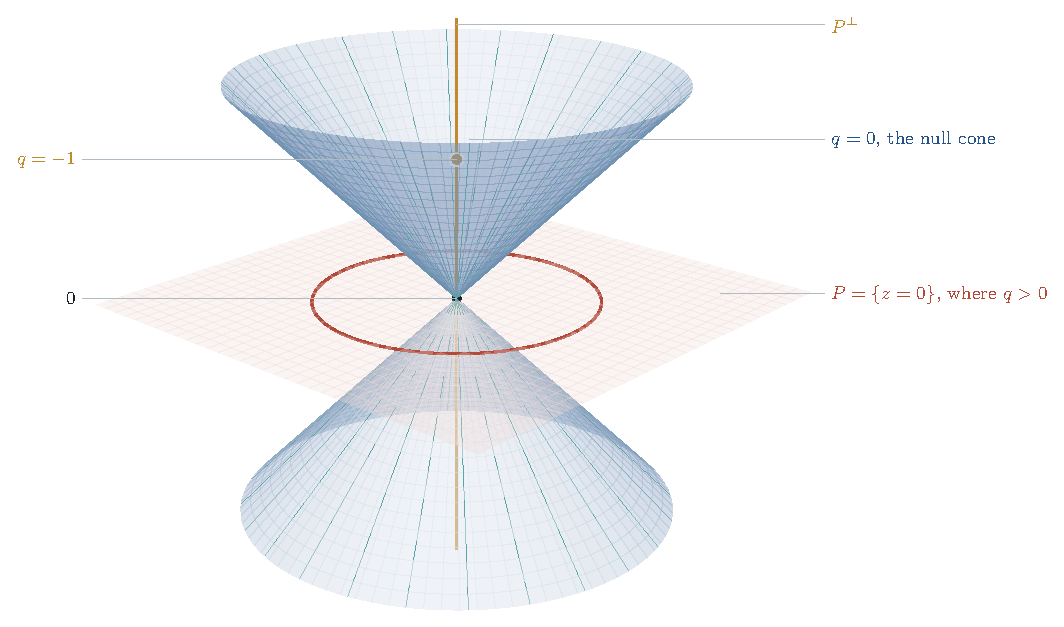
\includegraphics[width=0.88\textwidth]{fig_lightcone}
\caption{The geometry the Kuga--Satake construction starts from, in the
smallest case $b=3$. The quadratic form is $q=x^{2}+y^{2}-z^{2}$ of signature
$(2,1)$, with its null cone; the horizontal plane $P=\{z=0\}$ is positive
definite and meets the cone only at the origin. The construction needs such a
plane, and it gets one from \Cref{setup:k3type}: $P=\langle\Re\sigma,
\Im\sigma\rangle$ for the period $\sigma$ spanning $T^{2,0}$. An orthonormal
basis $e_{1},e_{2}$ of $P$ gives $J=e_{1}e_{2}$ with $J^{2}=-1$, by
\Cref{lem:cliffJ}, and $J$ is the complex structure on
$\mathrm{KS}(T)$. Positive definite planes correspond to the points of one
sheet of the hyperboloid $q=-1$, which is the period domain. The hypothesis
that makes all of this available is $\dim T^{2,0}=1$, and by
\Cref{prop:normpart} an abelian variety of Weil type supplies it only when
$n=1$.}
\label{fig:ks}
\end{figure}

\section{What is left}\label{sec:reduction}

This section assembles the obstructions into a statement about where the Hodge
conjecture can still be attacked. The statement is an equivalence and not a
reduction, in the sense that neither side is easier than the other; its value
is that it names the single place where a new idea has to enter, and
\Cref{thm:hyperplane} says that the classical inductive handle is blind
exactly there.

\subsection{Reduction to primitive classes}

\begin{proposition}[Lefschetz decomposition of Hodge classes]%
\label{prop:lefschetzdecomp}
Let $X$ be smooth projective of dimension $d$ with ample class $L$. Every
$\alpha\in\Hdg^{p}(X)$ can be written
\[
  \alpha=\sum_{r\ge\max(0,\,p-d+p)}L^{r}\beta_{r},
  \qquad
  \beta_{r}\in\Hdg^{p-r}(X)\cap H^{2p-2r}_{\mathrm{prim}}(X,\QQ),
\]
and the $\beta_{r}$ are uniquely determined. Consequently the Hodge conjecture
holds for $X$ if and only if every primitive rational Hodge class on $X$ is
algebraic.\footnote{The rationality of $L$ is what makes the primitive
parts rational. For a real K\"ahler class that is not a multiple of a rational
one the primitive subspaces are real but not rational, and a rational Hodge
class need not decompose into rational primitive pieces.}
\end{proposition}

\begin{proof}
The Lefschetz decomposition
$H^{k}(X,\QQ)=\bigoplus_{r}L^{r}H^{k-2r}_{\mathrm{prim}}(X,\QQ)$ is a
decomposition of rational Hodge structures, because $L$ is of type $(1,1)$ and
the primitive parts are kernels of morphisms of Hodge structures. A Hodge
class therefore has Hodge classes as its components. For the last statement,
if each primitive $\beta_{r}$ is algebraic then so is $L^{r}\beta_{r}$, since
$L$ is algebraic and algebraic classes form a subring, and hence so is
$\alpha$; the converse is trivial.
\end{proof}

\subsection{The equivalence}

\begin{theorem}\label{thm:equivalence}
The following are equivalent.
\begin{enumerate}[label=\textup{(\roman*)}]
\item The Hodge conjecture holds for every smooth complex projective variety.
\item The Lefschetz standard conjecture $B(X)$ holds for every smooth complex
  projective variety $X$, and every primitive rational Hodge class of middle
  degree on every smooth complex projective variety of even dimension is
  algebraic.
\end{enumerate}
\end{theorem}

\begin{proof}
(i) implies (ii). The second half of (ii) is a special case of (i). For
$B(X)$, the Hodge conjecture for $X\times X$ implies that the K\"unneth
components of the class of the diagonal that realise $\Lambda$ are algebraic:
$\Lambda$ is a morphism of Hodge structures of bidegree $(-1,-1)$, hence is
given by a Hodge class on $X\times X$ by the standard correspondence between
morphisms of Hodge structures and Hodge classes on the product, and (i)
applied to $X\times X$ makes that class algebraic. This is Kleiman's argument
\cite[\S2]{Kle68}.

(ii) implies (i). We argue by induction on $d=\dim X$. For $d\le1$ the Hodge
conjecture is classical. Let $d\ge2$ and assume the conjecture for all smooth
projective varieties of dimension less than $d$. By
\Cref{prop:lefschetzdecomp} it suffices to prove that a primitive Hodge class
$\alpha\in H^{2p}(X,\QQ)$ is algebraic, and by hard Lefschetz we may assume
$2p\le d$.

If $2p=d$, then $\alpha$ is a primitive Hodge class of middle degree on a
variety of even dimension, so it is algebraic by the second half of (ii).

If $2p<d$, choose a smooth hypersurface $Y\in|mH|$ for an ample $H$ and
$m\gg0$, which exists by Bertini, and put $L=c_{1}(\cO_{X}(Y))$. Since
$2p\le d-2$, \Cref{thm:LHT} makes $j^{*}\colon H^{2p}(X,\QQ)\to H^{2p}(Y,\QQ)$
an isomorphism, and $j^{*}\alpha$ is a rational Hodge class on $Y$ because
$j^{*}$ is a morphism of Hodge structures. As $\dim Y=d-1<d$, the inductive
hypothesis makes $j^{*}\alpha$ algebraic, say $j^{*}\alpha=\cl(W)$. Then
$\cl(j_{*}W)=j_{*}j^{*}\alpha=L\alpha$ by \Cref{lem:gysinrestrict}, so
$L\alpha$ is algebraic. By $B(X)$ the operator $\Lambda$ carries algebraic
classes to algebraic classes, and by \Cref{lem:LambdaL},
$\alpha=(d-2p)^{-1}\Lambda(L\alpha)$, which is therefore algebraic. Note
$d-2p\ge2$, so the scalar is nonzero.
\end{proof}

\begin{remark}[This is not a simplification]\label{rem:notsimpler}
Both halves of (ii) are open, and $B(X)$ is itself a consequence of (i), so
\Cref{thm:equivalence} does not reduce the problem to something smaller. What
it does is locate the difficulty. The induction in the proof of (ii) implies
(i) runs smoothly through every degree except the middle one, where it stops
and hands the work to the hypothesis; and \Cref{thm:hyperplane} says that the
step it uses below the middle degree, restriction to a hypersurface, returns
zero at the middle degree, so the induction cannot be extended to cover it by
any refinement of the same step.
\end{remark}

\begin{corollary}[Where a new idea must enter]\label{cor:whereidea}
Any proof of the Hodge conjecture must, at some point, produce an algebraic
cycle representing a primitive Hodge class of middle degree on a variety of
even dimension, by a method that does not factor through restriction to
hyperplane sections of that variety.
\end{corollary}

\begin{proof}
Immediate from \Cref{thm:equivalence} and \Cref{cor:blind}.
\end{proof}

\begin{remark}[Methods that do not factor through hyperplane sections]%
\label{rem:othermethods}
\Cref{cor:whereidea} is not a statement that the conjecture is unapproachable,
and we list the known methods that are outside its scope, since they are where
the successful cases come from. The Kuga--Satake construction replaces a
weight-two Hodge structure of K3 type by the $H^{1}$ of an abelian variety, and
the class it produces is of type $(1,1)$, hence algebraic by Lefschetz; this
is not a restriction to a subvariety and is untouched. Degenerations and
limits of Hodge structures move the variety rather than cutting it.
Correspondences from other varieties, of which the Kuga--Satake construction
is one instance and Markman's construction another, are also outside the
scope. Finally, arguments through the coniveau filtration, which show that a
class supported on a proper closed subvariety is controlled by that
subvariety, are compatible with everything here: they lower the dimension
legitimately, because the class is actually supported on the smaller variety,
which is exactly what a primitive coniveau-zero class is not.
\end{remark}

\begin{figure}[htbp]
\centering
  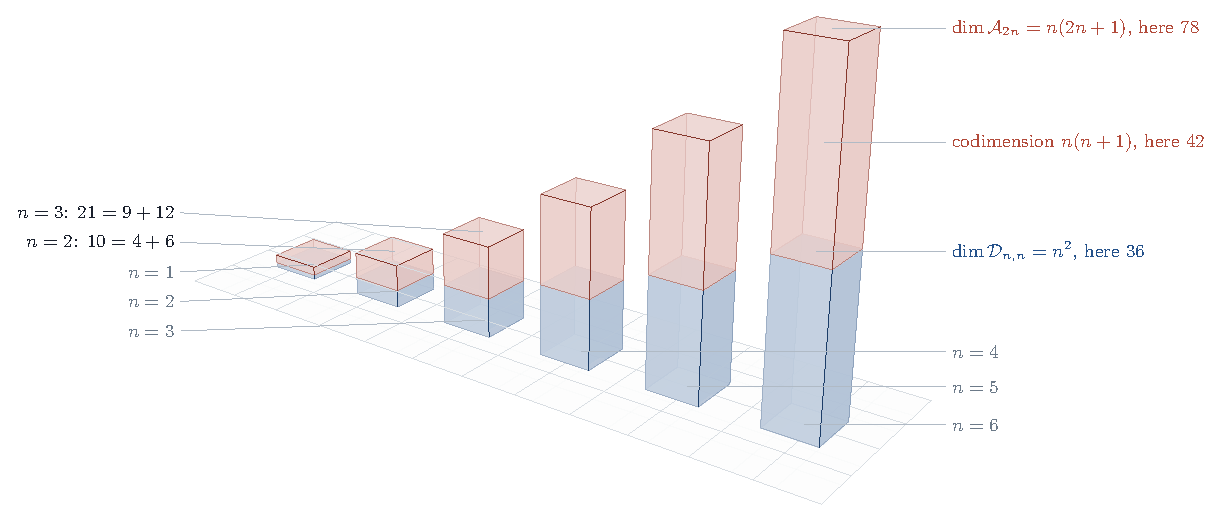
\includegraphics[width=0.92\textwidth]{fig_moduli}
\caption{The parameter count behind \Cref{thm:equivalence}. For
$n=1,\dots,6$ each prism has the height $n(2n+1)$ of the moduli of principally
polarised abelian $2n$-folds; its lower part, of height $n^{2}$, is the Weil
family of \Cref{prop:weildomain}, and its upper part is the codimension
$n(n+1)$. The gap widens quadratically, so the Weil locus is thin,
and by \Cref{cor:weilalgebraic} it is an algebraic subvariety. Both facts
matter for what is left: the locus one would have to deform along is small and
is a variety, and neither of those things produces a cycle on it.}
\label{fig:roadmap}
\end{figure}

\section{What a construction must break, and how Markman breaks it}
\label{sec:escape}

\Cref{thm:character} says that a $\Kx$-eigenclass for the norm character has no
component along the Weil line.%
\footnote{The three hypotheses below are not independent in spirit. A construction that imports its input from projective space will normally be equivariant for whatever acts on the input, and an equivariant construction will normally return a single eigenclass, so the three tend to hold or fail together. What \Cref{prop:whichescaped} records is that Markman's construction fails all three at once, and that no two of them can be dropped in isolation.} It is natural to ask what the contrapositive
demands of a construction that does reach the Weil line, and the answer is
sharper than one might expect: the demand is not on the size of the object, nor
on the ambient geometry, nor on any dimension count, but on the way the object
transforms. This section states that demand, and then shows that the one
construction known to meet it, Markman's, meets it in a specific and
reproducible way. The section is the most useful one in the paper for anybody
who wants to build something new, so we have tried to make the requirement
concrete rather than merely negative.

\subsection{The orbit criterion}

\begin{proposition}[Weil classes generate a plane]\label{prop:orbitplane}
Let $(A,\iota,\eta)$ be of $(K,-1,n)$-Weil type and let $\alpha\in\HW(A)$ be
nonzero. Then
\[
  \mathrm{span}_{\QQ}\bigl\{\iota(\tau)^{*}\alpha\;:\;\tau\in\Kx\bigr\}
  \;=\;\HW(A),
\]
a two-dimensional $\QQ$-vector space, and as a representation of $\Kx$ it is
irreducible over $\QQ$.
\end{proposition}

\begin{proof}
By \Cref{prop:weilline}(i) the space $\HW(A)$ is free of rank one over $K$, and
$\iota(\tau)^{*}$ acts on it as multiplication by the scalar $\tau^{2n}\in K$.
Hence the span in question is $S\cdot\alpha$, where
$S=\mathrm{span}_{\QQ}\{\tau^{2n}:\tau\in\Kx\}\subseteq K$. Taking $\tau=1$
shows $1\in S$. By the argument in the proof of \Cref{lem:charsdiffer} the map
$c(\tau)=\tau/\bbar{\tau}$ has infinite image while $\mu(K)$ is finite, so there
is $\tau_{0}$ with $(\tau_{0}/\bbar{\tau_{0}})^{2n}\ne1$, that is with
$\tau_{0}^{2n}\ne\bbar{\tau_{0}}^{\,2n}$, that is with $\tau_{0}^{2n}\notin\QQ$.
Then $S\supseteq\QQ+\QQ\tau_{0}^{2n}=K$, so $S=K$ and the span is
$K\alpha=\HW(A)$.

Irreducibility: a proper nonzero $\Kx$-stable $\QQ$-subspace would be a line,
on which $\Kx$ would act by a $\QQ$-valued character, forcing
$\tau^{2n}\in\QQ$ for all $\tau$, which we have just excluded.
\end{proof}

\begin{corollary}[The orbit criterion]\label{cor:orbitcriterion}
Let $\cE$ be an object of $D^{b}(A)$, or $Z$ a cycle in $\CH^{n}(A)_{\QQ}$,
whose class $\ch_{n}(\cE)$, respectively $\cl(Z)$, is a nonzero Weil class.
Then there is no function $\chi\colon\Kx\to\QQ$ with
\[
  \iota(\tau)^{*}\ch_{n}(\cE)=\chi(\tau)\,\ch_{n}(\cE)
  \qquad\text{for all }\tau\in\Kx .
\]
Equivalently, the $\Kx$-orbit of the class spans a plane and not a line.
\end{corollary}

\begin{proof}
Such a $\chi$ would make $\QQ\cdot\ch_{n}(\cE)$ a $\Kx$-stable line inside
$\HW(A)$, contradicting \Cref{prop:orbitplane}.
\end{proof}

\Cref{cor:orbitcriterion} is the precise sense in which a construction must
break equivariance. Here is what it forbids. Suppose a
construction assigns to the data $(A,\iota,\eta)$ an object $\cE(A,\iota,\eta)$
in a way that is natural, meaning that an isomorphism of the data induces an
isomorphism of the objects. The endomorphism $\iota(\tau)$ is, for $\tau$ in
the order, an isogeny of $A$ commuting with $\iota$ and multiplying $\eta$ by
$\Nm(\tau)$; naturality then forces
$\iota(\tau)^{*}\cE\cong\cE$ up to the normalisation that the polarisation
change imposes, and the induced relation on $\ch_{n}$ is precisely of the
forbidden form $\chi(\tau)\ch_{n}(\cE)$ with $\chi$ a power of the norm. So:

\begin{quote}
\emph{No construction that is natural in the $K$-action, taken alone, can
produce a Weil class. The construction must depend on a choice that
$\Gal(K/\QQ)$ moves.}
\end{quote}

The rest of this section shows what such a choice looks like in practice.

\subsection{The two conjugate isotropic subspaces}

The choice that $\Gal(K/\QQ)$ moves is visible already in \Cref{sec:characters}
and we name it here. The splitting
$V_{\CC}=V_{+}\oplus V_{-}$ of \eqref{eq:Vsplit} is defined over $K$ and not
over $\QQ$: conjugation interchanges the two summands. Consequently
$\bigwedge^{2n}V_{+}$ and $\bigwedge^{2n}V_{-}$ are individually defined over
$K$, and only their sum is rational. A class in $\HW(A)$ is of the form
$w+\bbar{w}$ with $w\in\bigwedge^{2n}V_{+}$, and the two summands are the two
conjugate halves.

\begin{definition}[Conjugate pair data]\label{def:conjpair}
By \emph{conjugate pair data} for $(A,\iota,\eta)$ we mean an ordered choice of
one of the two summands $V_{\pm}$, equivalently an ordered choice of one of the
two embeddings $K\hookrightarrow\CC$, equivalently a choice of one of the two
points of a $\Gal(K/\QQ)$-orbit of size two attached to the $K$-structure.
\end{definition}

\begin{proposition}[Corestriction produces the plane]\label{prop:corestriction}
Let $w\in\bigwedge^{2n}V_{+}$ be nonzero. Then $w+\bbar{w}$ and
$\sqrt{-d}\,(w-\bbar{w})$ lie in $\HW(A)$ and span it over $\QQ$. In
particular, a rational class in the Weil line is exactly a
$\Gal(K/\QQ)$-corestriction of a class in one conjugate half, and any
construction producing such a class must produce, in effect, a pair of
conjugate inputs and combine them.
\end{proposition}

\begin{proof}
Both displayed elements are fixed by conjugation, hence rational, and both lie
in $\bigwedge^{2n}V_{+}\oplus\bigwedge^{2n}V_{-}$ by construction, hence in
$\HW(A)$ by \Cref{def:weilline}. They are linearly independent over $\QQ$
because $w$ and $\bbar{w}$ are linearly independent over $\CC$, and $\HW(A)$ has
dimension two by \Cref{prop:weilline}(i).
\end{proof}

This is the design principle. A construction reaching the Weil line has to be,
in a suitable sense, \emph{bilinear in the two conjugate halves}: it must take
one input attached to $V_{+}$ and one attached to $V_{-}$ and pair them. A
construction fed a single $K$-invariant input cannot do this, which is
\Cref{cor:orbitcriterion} again.

\subsection{How Markman's construction meets the criterion}

Markman's work \cite{Mar25a,Mar25b} is the only construction we know of that
produces Weil classes, and it meets the criterion exactly in the manner just
described. We set out the relevant structure; the details are in
\cite{Mar25b}, and we claim no part of them.

The construction does not begin on $A$ or on $\Av$. It begins on an abelian
$n$-fold $X$, that is, on a variety of half the dimension of $A$. Inside
$H^{\mathrm{ev}}(X,\QQ)$ one selects a plane $P$ spanned by Hodge classes, and
one requires that $P$ meet the spinor variety of even pure spinors in two
points. Those two points are conjugate over the imaginary quadratic field $K$;
they correspond to two maximal isotropic subspaces $W_{1}$ and $W_{2}$ that are
interchanged by $\Gal(K/\QQ)$. This is the conjugate pair data of
\Cref{def:conjpair}, realised concretely.

To each of the two points one attaches a \emph{secant sheaf} on $X$: a coherent
sheaf whose Chern character is the corresponding point of $P$. In the worked
case where $X$ is the Jacobian of a curve of genus three, the secant sheaf is
$\mathcal{I}_{\cup C_{i}}(\Theta)$, the twist by the theta bundle of the ideal
sheaf of a union of translates of the Abel--Jacobi image of the curve. Call the
two sheaves $\cF_{1}$ and $\cF_{2}$.

The abelian variety of Weil type is then $A=X\times\widehat{X}$, of dimension
$2n$, with its $K$-action and polarisation inherited from $P$. The object that
carries the Weil class is
\begin{equation}\label{eq:markmanobject}
  E=\Phi\bigl(\cF_{1}^{\vee}\boxtimes\cF_{2}\bigr),
\end{equation}
where $\Phi\colon D^{b}(X\times X)\to D^{b}(X\times\widehat{X})$ is Orlov's
derived equivalence. One then shows that the characteristic class $\kappa(E)$
remains of Hodge type under every deformation of $X\times\widehat{X}$ as a
polarised abelian $2n$-fold of Weil type, which is what makes the class
algebraic on the whole family. The conclusion in \cite{Mar25b} is the
algebraicity of the Weil classes for abelian sixfolds of Weil type of
discriminant $-1$, and, through Schoen's degeneration argument, for all abelian
fourfolds of Weil type, whence the Hodge conjecture for abelian fourfolds.

\begin{proposition}[Which hypotheses are escaped]\label{prop:whichescaped}
The object \eqref{eq:markmanobject} satisfies none of the hypotheses of
\Cref{thm:divisor} and does not satisfy the hypothesis of
\Cref{thm:equivsuffices}. Specifically:
\begin{enumerate}[label=\textup{(\roman*)}]
\item \emph{The source is not a projective space.} The input
  $\cF_{1}^{\vee}\boxtimes\cF_{2}$ lives on $X\times X$, an abelian variety.
  The proof of \Cref{thm:divisor} used that $H^{*}(\PP^{N-1},\QQ)$ is generated
  in degree two, so that $\ch$ of any object is a polynomial in the hyperplane
  class. The cohomology of $X\times X$ is not generated in degree two: it
  contains K\"unneth classes of every degree, and $\ch(\cF_{1}^{\vee}\boxtimes\cF_{2})$
  is not confined to any divisor subring.
\item \emph{The transform is not $\Phi_{\cP}$ on $A\times\Av$.} The relevant
  equivalence is between $D^{b}(X\times X)$ and $D^{b}(X\times\widehat{X})$,
  and \Cref{thm:fmtheta}, which computes the transform with Poincar\'e kernel
  on powers of the polarisation of $A$, says nothing about it.
\item \emph{The construction is not $K$-equivariant.} The two tensor factors
  of \eqref{eq:markmanobject} carry the two conjugate points of
  $P\cap(\text{spinor variety})$, one each. Interchanging them is the action of
  the nontrivial element of $\Gal(K/\QQ)$, and it exchanges $E$ with a
  different object. Hence $\ch_{n}(E)$ is not a $\Kx$-eigenclass for the norm,
  and \Cref{cor:orbitcriterion} is satisfied rather than violated.
\end{enumerate}
\end{proposition}

\begin{proof}
(i) and (ii) are a comparison of hypotheses and require no argument beyond
reading \eqref{eq:markmanobject}. For (iii), if $\ch_{n}(E)$ were an eigenclass
for the norm then by \Cref{cor:equivariant} it would have zero component along
the Weil line, whereas Markman establishes that it spans one \cite{Mar25b}.
\end{proof}

\begin{remark}[The lesson for the secant idea]\label{rem:secantlesson}
We are explicit here, because the point is easy to miss and is the reason
this section exists. The idea of using secant geometry to produce Weil classes
is not what fails. Markman's construction is a secant construction, and it
works. What fails is siting the secant geometry on the dual $\Av$ of the
$2n$-fold inside an ambient projective space, and transporting by the
Poincar\'e kernel. That siting has three defects at once, by
\Cref{prop:whichescaped}: it puts the input where the cohomology is generated
by a divisor, it uses the transform for which \Cref{thm:fmtheta} applies, and
it feeds the construction $K$-invariant data, since a secant variety of a
$K$-invariant subvariety is $K$-invariant. Moving the secant geometry down to
an abelian $n$-fold repairs all three, and it does so because the halving of
the dimension is what makes room for the two conjugate inputs.
\end{remark}

\subsection{What would be needed above the known range}

We can now state precisely what a construction for the cases that remain open
would have to supply. The known range is $n=2$, all discriminants, and $n=3$
with discriminant $-1$; see \cite{Mar25b} and, for a different route at
discriminant $1$, \cite{FF26}.

\begin{question}\label{q:higher}
Fix $n\ge4$ and an imaginary quadratic field $K$. Does there exist an abelian
$n$-fold $X$, a plane $P\subset H^{\mathrm{ev}}(X,\QQ)$ spanned by Hodge
classes meeting the spinor variety in two points conjugate over $K$, secant
sheaves $\cF_{1},\cF_{2}$ on $X$ realising those two points, and a deformation
argument showing that $\kappa\bigl(\Phi(\cF_{1}^{\vee}\boxtimes\cF_{2})\bigr)$
remains of Hodge type across the moduli of polarised abelian $2n$-folds of
Weil type with multiplication by $K$?
\end{question}

Each of the four ingredients is a concrete demand and none is obviously out of
reach; what is absent at present is the analogue of the genus three Jacobian,
namely a family of abelian $n$-folds in which the plane $P$ and the two secant
sheaves can be written down. By \Cref{cor:orbitcriterion} any successful answer
must, however it is phrased, be bilinear in a pair of conjugate inputs, because
that is the only way a rational class can acquire a $\Kx$-orbit of dimension
two. We offer \Cref{q:higher} as the sharpest form we can give of what is left
on the abelian side, and we note that it is a question about writing down one
sheaf on one abelian variety, not a question about a general mechanism.

\begin{figure}[htbp]
\centering
  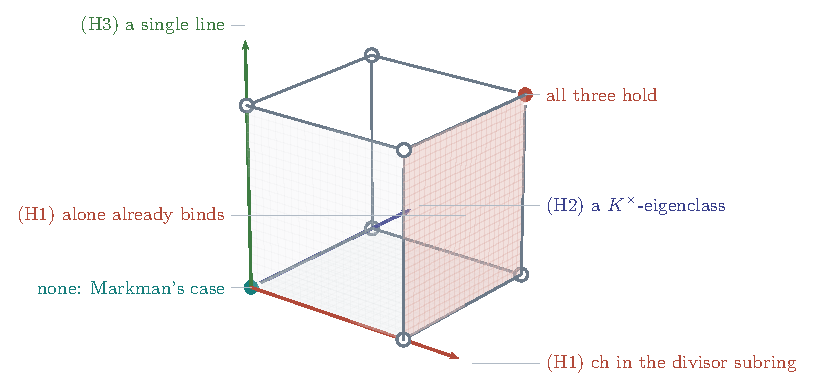
\includegraphics[width=0.97\textwidth]{fig_escape}
\caption{The eight positions a secant construction can occupy, drawn as the
Boolean lattice of subsets of the three hypotheses isolated in
\Cref{prop:whichescaped}: (H1) the Chern character of the input lies in the
subring generated by divisor classes, (H2) the output is a $\Kx$-eigenclass,
(H3) the output spans a single line rather than a plane. A construction
satisfying all three sits at the top vertex, where \Cref{thm:divisor} and
\Cref{thm:character} both apply; the shaded face is where (H1) alone already
binds. Markman's construction sits at the bottom vertex, satisfying none of
the three, which is why nothing here bears on it, and the Weil line needs a
plane by \Cref{prop:orbitplane}.}
\label{fig:escape}
\end{figure}

\section{An explicit secant plane in every dimension}\label{sec:construction}

\Cref{q:higher} asks for four things: an abelian $n$-fold $X$, a plane
$P\subset H^{\mathrm{ev}}(X,\QQ)$ of Hodge classes meeting the spinor variety
in two points conjugate over $K$, a pair of secant sheaves realising the
plane, and a deformation argument. This section supplies the first two in
closed form, for every $n\ge2$ and every imaginary quadratic $K$, and reduces
the third to an explicit equation on a Chern character. The fourth is
untouched and is the hardest of the four; we say so at the end.

The framework is Markman's: the Weil structure on $X\times\widehat{X}$
obtained by embedding $K$ into $\End^{0}(X\times\widehat{X})$, and the
notion of a $K$-secant sheaf whose Chern character lies in a plane meeting
the spinor variety at two conjugate points, are introduced in
\cite{Mar25a,Mar25b}, and the deformation step that finishes the argument
at $n=3$ is his. What we do here is write the first two ingredients out in
closed form, uniformly in $n$, $K$ and the discriminant, so that the third
becomes a finite system; we claim nothing beyond that.
What follows is elementary once set up, and we were surprised that it comes
out in closed form. The reason it does is that the two conjugate isotropic
subspaces demanded by \Cref{cor:orbitcriterion} can be produced by a single
element of the N\'eron--Severi group, and that the pure spinor of the graph of
a two-form is the exponential of that form.

\subsection{The Weil structure}

\begin{setupenv}\label{setup:construction}
Let $X$ be a complex abelian variety of dimension $n$ with
$H_{1}(X,\QQ)=U$ of dimension $2n$ and complex structure $J$ on
$U\otimes\RR$. Let $d$ be a squarefree positive integer, $s=\sqrt{-d}$ and
$K=\QQ(s)$. Let $\beta\in\NS(X)\otimes\QQ$ be nondegenerate, regarded as an
alternating form on $U$, so that the Riemann relation $J^{\top}\beta J=\beta$
holds, and write $\phi_{\beta}\colon X\to\widehat{X}$ for the associated
isogeny. Put
\[
  A=X\times\widehat{X},\qquad \dim A=2n,\qquad
  H_{1}(A,\QQ)=U\oplus U^{\vee},
\]
and let
\begin{equation}\label{eq:Mdef}
  M=\begin{pmatrix}0 & -\beta^{-1}\\[2pt] d\,\beta & 0\end{pmatrix}
  \in\End^{0}(A),
\end{equation}
acting on $H_{1}(A,\QQ)=U\oplus U^{\vee}$ by
$(u,\phi)\mapsto(-\beta^{-1}\phi,\;d\,\beta u)$.%
\footnote{The placement of the factor $d$ is a convention, and it has to be
made once and kept. The endomorphism $\begin{psmallmatrix}0&-d\beta^{-1}\\
\beta&0\end{psmallmatrix}$ also squares to $-d$ and also commutes with the
complex structure, and it defines a Weil structure on the same $A$; but it
is a different embedding of $K$, its eigenspaces are the graphs of
$\mp s\beta/d$ rather than of $\mp s\beta$, its polarisation is
$\beta+d\widehat\beta$ rather than $d\beta+\widehat\beta$, and the class in
$\bigwedge^{2}V_{+}\oplus\bigwedge^{2}V_{-}$ it produces is
$\beta-d\widehat\beta$ rather than $\gamma=d\beta-\widehat\beta$. The
convention of \eqref{eq:Mdef} is the one whose action on cohomology is
$x\mapsto-Bx$, $\xi\mapsto dB^{-1}\xi$ in the proof of
\Cref{thm:splitclosed}, and it is the one every script uses; item (XI) of
\Cref{sec:verification} checks the three eigenvalues that pin it down, and
item (XXV) shows what goes wrong if the two are mixed: the space of
polarised deformations killing the Weil line then has dimension
$n(n+1)/2$ instead of $n^{2}$. For $d=1$ the two conventions coincide.}
\end{setupenv}

\begin{theorem}[An explicit Weil structure]\label{thm:explicitweil}
In \Cref{setup:construction}:
\begin{enumerate}[label=\textup{(\roman*)}]
\item $M^{2}=-d$, so $\iota(s)=M$ defines an embedding
  $\iota\colon K\hookrightarrow\End^{0}(A)$;
\item $M$ commutes with the complex structure of $A$, and this holds exactly
  because $\beta$ satisfies the Riemann relation, that is because
  $\beta\in\NS(X)\otimes\QQ$;
\item $M$ acts on $H^{1,0}(A)$ with eigenvalues $s$ and $-s$, each of
  multiplicity $n$, so $(A,\iota,\eta)$ is of $(K,-1,n)$-Weil type for a
  suitable polarisation $\eta$;
\item the eigenspaces $W_{\pm}\subset H_{1}(A,\CC)$ of $M$ for $\pm s$ are
  maximal isotropic for the canonical pairing on $U\oplus U^{\vee}$, are
  interchanged by complex conjugation, and are the graphs of the two-forms
  $\mp s\beta$.
\end{enumerate}
\end{theorem}

\begin{proof}
(i) Block multiplication gives
$M^{2}=\mathrm{diag}(-\beta^{-1}\,d\beta,\;-d\beta\,\beta^{-1})=-d\cdot\mathrm{id}$.

(ii) The complex structure of $A=X\times\widehat{X}$ is
$J_{A}=\mathrm{diag}(J,-J^{\top})$. The relation $MJ_{A}=J_{A}M$ amounts to
the two identities $d\beta J=-dJ^{\top}\beta$ and
$-\beta^{-1}(-J^{\top})=J(-\beta^{-1})$, and each is equivalent to
$\beta J=-J^{\top}\beta$. That is exactly the Riemann relation: from
$J^{\top}\beta J=\beta$ and $J^{2}=-1$ one gets
$J^{\top}\beta=\beta J^{-1}=-\beta J$, as required. Conversely
$\beta J=-J^{\top}\beta$ gives $J^{\top}\beta J=-\beta J J=\beta$.

(iii) $M$ is block anti-diagonal and $H^{1,0}(A)=H^{1,0}(X)\oplus
H^{1,0}(\widehat{X})$ with both summands of dimension $n$, and $M$ exchanges
them. If $M(x,y)=\lambda(x,y)$ then $-\beta^{-1}y=\lambda x$ and
$d\beta x=\lambda y$, so $y=d\beta x/\lambda$ and, substituting,
$-dx/\lambda=\lambda x$, that is $\lambda^{2}=-d$. For each of
the two values of $\lambda$ the assignment $x\mapsto(x,d\beta x/\lambda)$ is an
isomorphism from $H^{1,0}(X)$ onto the $\lambda$-eigenspace, which is
therefore of dimension $n$. That is the balanced signature of
\Cref{def:weiltype}(ii). For (iii) of that definition one takes for $\eta$ the
polarisation of $A$ obtained from the canonical principal polarisation of
$X\times\widehat{X}$ twisted so that the Rosati involution sends $M$ to $-M$;
this is possible because $\beta$ is symmetric under the Rosati involution of
$X$, being a class in $\NS$.

(iv) The same computation identifies $W_{\lambda}=\{(x,d\beta x/\lambda)\}$,
the graph of the form $d\beta/\lambda$, and
$d\beta/\lambda=d\beta/(\pm s)=\mp s\beta$ since $d/s=-s$. The canonical
pairing on $U\oplus U^{\vee}$ is
$\langle(x,\xi),(x',\xi')\rangle=\xi'(x)+\xi(x')$, and on the graph it gives
$d\beta(x',x)/\lambda+d\beta(x,x')/\lambda=0$ because $\beta$ is alternating; so
$W_{\lambda}$ is isotropic, and it has dimension $2n$, half of
$\dim(U\oplus U^{\vee})=4n$, hence is maximal. Conjugation sends $s$ to $-s$
and so interchanges the two.
\end{proof}

\begin{remark}\label{rem:abundant}
\Cref{thm:explicitweil} says that abelian $2n$-folds of Weil type of the split
form $X\times\widehat{X}$ exist for every $n$, every imaginary quadratic $K$
and every polarised abelian $n$-fold $X$, and that the Weil structure is
written down by one element of $\NS(X)$. These are not general members of the
moduli of Weil type, and the Weil classes on them are of interest precisely
because Markman's deformation argument propagates algebraicity from them to
the general member; see \Cref{rem:deformation} below.
\end{remark}

\subsection{The plane}

Write $t=\beta\in\NS(X)\otimes\QQ$, so that by
\Cref{thm:explicitweil}(iv) the two conjugate maximal isotropic subspaces are
the graphs of $\mp s\,t$; the letter $t$ is kept because everything below
holds for any nondegenerate $t\in\NS(X)\otimes\QQ$. The pure spinor attached to the graph of a two-form
$\omega$ is $e^{\omega}$, so the two conjugate points of the even spinor
variety determined by the Weil structure are $[e^{-st}]$ and $[e^{st}]$.

\begin{definition}[The secant plane]\label{def:secantplane}
With $t$ and $d$ as above, put
\begin{equation}\label{eq:uv}
  u_{t}=\sum_{j\ge0}\frac{(-d)^{j}}{(2j)!}\,t^{2j},
  \qquad
  v_{t}=\sum_{j\ge0}\frac{(-d)^{j}}{(2j+1)!}\,t^{2j+1},
\end{equation}
both sums being finite because $t^{k}=0$ for $k>n$, and let
$P_{t}=\QQ u_{t}\oplus\QQ v_{t}\subset H^{\mathrm{ev}}(X,\QQ)$.
\end{definition}

\begin{theorem}[The plane is an explicit rational secant]\label{thm:plane}
With notation as above:
\begin{enumerate}[label=\textup{(\roman*)}]
\item $u_{t}$ and $v_{t}$ are rational Hodge classes, and
  $e^{\pm st}=u_{t}\pm s\,v_{t}$;
\item $P_{t}$ is a two-dimensional $\QQ$-subspace of $H^{\mathrm{ev}}(X,\QQ)$
  spanned by Hodge classes, and $\PP(P_{t})$ is a line defined over $\QQ$
  passing through the two conjugate points $[e^{\pm st}]$ of the even spinor
  variety;
\item that line is not contained in the spinor variety, so it meets it in
  exactly those two points.
\end{enumerate}
\end{theorem}

\begin{proof}
(i) Each $t^{k}$ is a rational Hodge class because $t\in\NS(X)\otimes\QQ$ is
of type $(1,1)$ and the algebraic classes form a subring. Separating
$e^{st}=\sum_{k}s^{k}t^{k}/k!$ into even and odd powers of $s$ and using
$s^{2j}=(-d)^{j}$, $s^{2j+1}=(-d)^{j}s$ gives $e^{st}=u_{t}+sv_{t}$, and
conjugating gives $e^{-st}=u_{t}-sv_{t}$.

(ii) The two elements are linearly independent over $\QQ$ because $u_{t}$ has
nonzero component in $H^{0}$ and $v_{t}$ does not, while $v_{t}\ne0$ since
$t\ne0$. From (i), both $e^{st}$ and $e^{-st}$ lie in $P_{t}\otimes K$, so
$\PP(P_{t})$ passes through the two points.

(iii) The even spinor variety is cut out by quadrics, by Cartan's description
of pure spinors, so a line either lies inside it or meets it in a subscheme of
length at most two. The point $[u_{t}]$ of $\PP(P_{t})$ is not a pure spinor:
a pure spinor with nonzero component in $H^{0}$ is a scalar multiple of
$e^{\omega}$ for a two-form $\omega$, and $u_{t}$ has zero component in
$H^{2}$ while its component in $H^{4}$ is $-\tfrac{d}{2}t^{2}\ne0$, whereas
$e^{\omega}$ with vanishing $H^{2}$ part is $1$. So the line is not contained
in the spinor variety, and the two points of (ii) exhaust the intersection.
\end{proof}

\begin{example}\label{ex:planes}
For $n=4$ and $d=1$,
$u_{t}=1-\tfrac{1}{2}t^{2}+\tfrac{1}{24}t^{4}$ and
$v_{t}=t-\tfrac{1}{6}t^{3}$. For $n=4$ and $d=3$,
$u_{t}=1-\tfrac{3}{2}t^{2}+\tfrac{3}{8}t^{4}$ and
$v_{t}=t-\tfrac{1}{2}t^{3}$. Both are visibly rational and visibly in the
subring generated by $t$.
\end{example}

\subsection{The Chern character equation}

We can now say exactly what a secant sheaf has to be. The following is the
substance of this section: the four demands of \Cref{q:higher} collapse, on
the sheaf side, to one equation with all invariants computed.

\begin{theorem}[The invariants of a secant sheaf]\label{thm:secantinvariants}
Let $X$, $t$, $d$ be as above and let $\cF$ be a coherent sheaf on $X$ with
$\ch(\cF)\in P_{t}$, say $\ch(\cF)=a\,u_{t}+b\,v_{t}$ with $a,b\in\QQ$. Then
\[
  \rk\cF=a,\qquad
  c_{1}(\cF)=b\,t,\qquad
  \ch_{2}(\cF)=-\tfrac{ad}{2}\,t^{2},\qquad
  c_{2}(\cF)=\tfrac{ad+b^{2}}{2}\,t^{2},
\]
and more generally $\ch_{k}(\cF)$ is the degree $k$ term of \eqref{eq:uv}
scaled by $a$ or $b$ according to the parity of $k$. The Bogomolov
discriminant is
\begin{equation}\label{eq:discnorm}
  \Delta(\cF)=2a\,c_{2}(\cF)-(a-1)c_{1}(\cF)^{2}
  =\Nm_{K/\QQ}\bigl(b+a s\bigr)\cdot t^{2}.
\end{equation}
In particular $\Delta(\cF)\cdot H^{n-2}>0$ for every ample $H$, so the
Bogomolov inequality places no obstruction on the existence of $\cF$.
\end{theorem}

\begin{proof}
The first four identities are read off from \eqref{eq:uv} degree by degree,
using $\ch_{2}=\tfrac12(c_{1}^{2}-2c_{2})$ to convert $\ch_{2}$ into $c_{2}$.
For \eqref{eq:discnorm},
\[
  2a\cdot\tfrac{ad+b^{2}}{2}t^{2}-(a-1)b^{2}t^{2}
  =\bigl(a^{2}d+ab^{2}-ab^{2}+b^{2}\bigr)t^{2}
  =\bigl(a^{2}d+b^{2}\bigr)t^{2},
\]
and $\Nm_{K/\QQ}(b+as)=(b+as)(b-as)=b^{2}+a^{2}d$. Positivity of the norm on
$\Kx$ and of $t^{2}H^{n-2}$ for $t$ in the positive cone give the last
assertion.
\end{proof}

\begin{remark}[The norm form as the discriminant]\label{rem:normdisc}
Identity \eqref{eq:discnorm} is the reason the construction has a chance at
all. The discriminant of the sheaf is the norm form of $K$ evaluated at the
coordinates of its Chern character in the plane. The two conjugate points of
the spinor variety are the two isotropic directions of that norm form after
extension to $K$, and the rational points of the plane are exactly the
non-isotropic ones. A sheaf therefore sits at a rational point of a conic
whose isotropic directions carry the Weil structure, which is the precise
sense in which the conjugate pair of \Cref{cor:orbitcriterion} is built into
the invariants rather than imposed on them.
\end{remark}

\begin{corollary}[The case of an abelian surface]\label{cor:surfacecase}
Let $n=2$, so $X$ is an abelian surface and $A=X\times\widehat{X}$ an abelian
fourfold of Weil type. A sheaf with $\ch(\cF)\in P_{t}$ has Mukai vector
$v(\cF)=(a,\,bt,\,-\tfrac{ad}{2}t^{2})$ and Mukai self-pairing
\[
  \langle v(\cF),v(\cF)\rangle=\Nm_{K/\QQ}(b+as)\cdot t^{2}>0 .
\]
\end{corollary}

\begin{proof}
On an abelian surface the Mukai pairing of $v=(r,c,e)$ with itself is
$c^{2}-2re$, which here is $b^{2}t^{2}-2a(-\tfrac{ad}{2}t^{2})=(b^{2}+a^{2}d)t^{2}$.
\end{proof}

\Cref{cor:surfacecase} is consistent with the known range: the positivity of
the Mukai self-pairing is exactly the numerical condition under which moduli
of stable sheaves on an abelian surface with a given Mukai vector are
non-empty, and $n=2$ is settled.

\subsection{The genus three case, and what the field predicts}

At $n=3$ the equation of \Cref{thm:secantinvariants} pins down the secant
sheaf far more tightly, and it reproduces the shape of the object Markman
uses. We record the computation because it is a check on the whole framework.

\begin{proposition}[Rank one at $n=3$]\label{prop:genus3}
Let $X$ be the Jacobian of a smooth curve of genus three, let $\Theta$ be the
theta divisor and $C\subset X$ the Abel--Jacobi curve, so that
$\Theta^{2}/2=[C]$. Take $t=\Theta$ and $a=1$ in
\Cref{thm:secantinvariants}. Then a rank one torsion-free sheaf $\cF$ with
$\ch(\cF)\in P_{\Theta}$ and $c_{1}(\cF)=b\Theta$ is of the form
$\cF=\mathcal{I}_{Z}(b\Theta)$ with
\[
  [Z]=\frac{b^{2}+d}{2}\,\Theta^{2}
     =\frac{b^{2}+d}{b^{2}}\cdot b^{2}[C].
\]
If $Z$ is a disjoint union of translates of $C$, the number of translates is
$m=(b^{2}+d)/b^{2}$, which is a positive integer precisely when $b^{2}\mid d$;
for $b=1$,
\[
  m=d+1 .
\]
\end{proposition}

\begin{proof}
A rank one torsion-free sheaf with $c_{1}=b\Theta$ on a smooth projective
threefold is $\mathcal{I}_{Z}(b\Theta)$ for a subscheme $Z$ of codimension at
least two, and
$\ch(\mathcal{I}_{Z}(b\Theta))=e^{b\Theta}-[Z]-(\text{terms in }H^{6})$.
Comparing the components in $H^{4}$ with \Cref{thm:secantinvariants} at $a=1$,
which gives $\ch_{2}=-\tfrac{d}{2}\Theta^{2}$, yields
$\tfrac{b^{2}}{2}\Theta^{2}-[Z]=-\tfrac{d}{2}\Theta^{2}$, that is
$[Z]=\tfrac{b^{2}+d}{2}\Theta^{2}$. The Poincar\'e formula
$\Theta^{g-1}/(g-1)!=[C]$ at $g=3$ reads $\Theta^{2}/2=[C]$, whence
$[Z]=(b^{2}+d)[C]$, and if $Z$ is $m$ translates of $C$ then $m=b^{2}+d$ when
$b=1$ and $m=(b^{2}+d)/b^{2}$ after dividing by the class of $b^{2}$
translates in general.
\end{proof}

\begin{table}[htbp]
\centering
\renewcommand{\arraystretch}{1.15}
\begin{tabular}{@{}rrrrrrr@{}}
\toprule
$d$ & $1$ & $2$ & $3$ & $5$ & $7$ & $11$ \\
\midrule
$m=d+1$ & $2$ & $3$ & $4$ & $6$ & $8$ & $12$ \\
\bottomrule
\end{tabular}
\caption{The number of translates of the Abel--Jacobi curve required at
$n=3$, $b=1$, as a function of the field $K=\QQ(\sqrt{-d})$, by
\Cref{prop:genus3}.}
\label{tab:translates}
\end{table}

\begin{remark}\label{rem:markmancheck}
The sheaf used in \cite{Mar25b} on a genus three Jacobian is
$\mathcal{I}_{\cup C_{i}}(\Theta)$, the twist by the theta bundle of the ideal
sheaf of a union of translates of the Abel--Jacobi curve. That is exactly the
shape \Cref{prop:genus3} forces, with the number of translates determined by
the field. We take this as evidence that the framework of this section is the
right one and not merely a consistent one.
\end{remark}

\subsection{The third ingredient, in every dimension}\label{ssec:thirdexists}

\Cref{thm:secantinvariants} says what a secant sheaf must look like. It does
not say that one exists, and at $n\ge4$ that is the question the section has so
far left open. We settle it here, and the answer is that the object exists on
every polarised abelian variety, in every dimension, for every imaginary
quadratic field, and that it can be assembled out of powers of a single line
bundle.

Two observations do the work. The first is that the object wanted is a
rational point of a plane, and a plane carries no preferred scale. If a
positive multiple of a rational point of $P_{t}$ is realised by a sheaf, then a
rational point of $P_{t}$ is realised by a sheaf, and since the Hodge
conjecture is a statement about classes with rational coefficients, replacing
$\omega$ by $M\omega$ costs nothing. The second is that once one is free to
clear denominators, the Chern characters of the powers of one line bundle
already span the subring in which the secant plane lives, because the matrix
expressing them in the basis $t^{k}/k!$ is a Vandermonde matrix on distinct
nodes.

What is missing is only the passage from a class in $K_{0}$ to a sheaf, and
for that the sign of the rank is the whole of the hypothesis.

\begin{lemma}[Positive rank is enough]\label{lem:posrank}
Let $Y$ be a smooth projective variety over a field and let $\alpha\in
K_{0}(Y)$ satisfy $\rk\alpha>0$. Then $\alpha=[\cF]$ for some coherent sheaf
$\cF$ on $Y$.
\end{lemma}

\begin{proof}
Write $m=\dim Y$ and $a=\rk\alpha\ge1$, and let $F^{c}K_{0}(Y)$ be the
topological filtration, the subgroup generated by the classes $[\cO_{Z}]$ of
closed integral subschemes $Z\subseteq Y$ of codimension at least $c$. Since
$Y$ is smooth, every coherent sheaf has a finite locally free resolution, so
$K_{0}(Y)=K_{0}'(Y)$ and the filtration is exhaustive with $F^{m+1}=0$;
moreover $F^{c}/F^{c+1}$ maps onto $\CH^{c}(Y)$ by sending the class of a sheaf
supported in codimension $c$ to its associated cycle, and $F^{1}$ is the kernel
of the rank while $F^{1}/F^{2}$ is $\Pic(Y)$ by the first Chern class
\cite[\S 15.1 and Ex.~15.1.5]{Ful98}. We construct coherent
sheaves $\cF_{c}$ of rank $a$ with $\alpha-[\cF_{c}]\in F^{c}$, by induction on
$c$.

Start at $c=2$. Let $L$ be a line bundle with $c_{1}(L)=c_{1}(\alpha)$ and set
$\cF_{2}=L\oplus\cO_{Y}^{\oplus(a-1)}$. Then $\alpha-[\cF_{2}]$ has rank zero
and first Chern class zero, hence lies in $F^{2}$.

For the inductive step let $\delta=\alpha-[\cF_{c}]\in F^{c}$ with $c\ge2$.
Modulo $F^{c+1}$ the class $\delta$ is a finite sum $\sum_{j}m_{j}
[\cO_{Z_{j}}]$ with $m_{j}\in\ZZ$ and $\codim Z_{j}=c$. The terms with
$m_{j}>0$ are removed by replacing $\cF_{c}$ with $\cF_{c}\oplus\bigoplus_{
m_{j}>0}\cO_{Z_{j}}^{\oplus m_{j}}$, which changes neither the rank nor the
codimension of the remaining difference. For a term with $m_{j}<0$ we must
subtract, and here the rank is used. The restriction $\cF_{c}\otimes
\cO_{Z_{j}}$ is a quotient of $\cF_{c}$ and has rank $a\ge1$ at the generic
point of the integral scheme $Z_{j}$; choosing a subsheaf of generic corank
one and dividing by it gives a surjection $\cF_{c}\twoheadrightarrow\cQ$ with
$\cQ$ of rank one on $Z_{j}$. Then $[\cQ]\in F^{c}$ with associated cycle
$[Z_{j}]$, so $[\cQ]-[\cO_{Z_{j}}]\in F^{c+1}$. The kernel of that surjection
is a coherent sheaf, still of rank $a$ because $\cQ$ is supported in positive
codimension, and its class is $[\cF_{c}]-[\cQ]$. Performing this $|m_{j}|$
times, and once for each $j$, produces $\cF_{c+1}$ with
$\alpha-[\cF_{c+1}]\in F^{c+1}$ and $\rk\cF_{c+1}=a$. At $c=m+1$ the
difference lies in $F^{m+1}=0$, so $\alpha=[\cF_{m+1}]$.
\end{proof}

\begin{theorem}[Secant sheaves exist in every dimension]\label{thm:secantexists}
Let $X$ be an abelian variety of dimension $n$, let $t\in\NS(X)\otimes\QQ$ be a
polarisation and let $d>0$. Let $p$ be a rational point of the secant plane
$P_{t}$ whose $u_{t}$ coordinate is positive. Then there are a positive
integer $M$, an integer $D>0$ with $Dt\in\NS(X)$, integers $n_{0},\dots,n_{n}$
and a coherent sheaf $\cF$ on $X$ such that, setting
\begin{equation}\label{eq:lbwitness}
  \alpha=\sum_{j=0}^{n}n_{j}\bigl[\cO_{X}(jDt)\bigr]\in K_{0}(X),
\end{equation}
one has $\alpha=[\cF]$ in $K_{0}(X)$, $\ch(\cF)=M\,p$ and
$\rk\cF=M\,a>0$, where $a$ is the $u_{t}$ coordinate of $p$. The integers $M$
and $n_{j}$ depend only on $n$, $d$ and the coordinates of $p$, and are
obtained by inverting one Vandermonde matrix. Moreover $Mp$ is again a
rational point of $P_{t}$; applying the statement to two linearly independent
rational points of $P_{t}$ produces a pair of coherent sheaves whose Chern
characters span $P_{t}$.
\end{theorem}

\begin{proof}
Scaling $p$ by a positive integer changes neither the hypothesis nor the
conclusion, so we may assume $p=au_{t}+bv_{t}$ with $a,b\in\ZZ$ and $a>0$.
Choose $D>0$ with $Dt\in\NS(X)$, so that $\cO_{X}(jDt)$ is a line bundle for
every $j\in\ZZ$.

Since $t$ is a polarisation, $t^{n}\ne0$ and $t^{n+1}=0$ in
$H^{\mathrm{ev}}(X,\QQ)$, so the $n+1$ classes $t^{k}/k!$ with $0\le k\le n$
are a basis of the subring $\QQ[t]$. In that basis
\[
  p=\sum_{k=0}^{n}c_{k}\,\frac{t^{k}}{k!},\qquad
  c_{k}=\begin{cases}a(-d)^{k/2}, & k\ \text{even},\\[2pt]
                     b(-d)^{(k-1)/2}, & k\ \text{odd},\end{cases}
\]
by \Cref{prop:notforbidden}(i), and all the $c_{k}$ are integers. On the other
side,
\[
  \ch\bigl(\cO_{X}(jDt)\bigr)=e^{jDt}=\sum_{k=0}^{n}(jD)^{k}\,\frac{t^{k}}{k!},
\]
so in the same basis the $n+1$ vectors $\ch(\cO_{X}(jDt))$ for $j=0,\dots,n$
are the columns of the Vandermonde matrix $\bigl((jD)^{k}\bigr)_{0\le j,k\le n}$
on the $n+1$ distinct nodes $0,D,2D,\dots,nD$. Its determinant is
$\prod_{0\le i<j\le n}(jD-iD)=D^{n(n+1)/2}\prod_{0\le i<j\le n}(j-i)\ne0$, so
the system
\[
  \sum_{j=0}^{n}x_{j}\,(jD)^{k}=c_{k}\qquad(0\le k\le n)
\]
has a unique solution $x\in\QQ^{n+1}$. Let $M$ be the least common multiple of
the denominators of the $x_{j}$ and put $n_{j}=Mx_{j}\in\ZZ$. With $\alpha$ as
in \eqref{eq:lbwitness},
\[
  \ch(\alpha)=\sum_{j}n_{j}e^{jDt}
  =\sum_{k=0}^{n}\Bigl(\sum_{j}Mx_{j}(jD)^{k}\Bigr)\frac{t^{k}}{k!}
  =M\sum_{k=0}^{n}c_{k}\frac{t^{k}}{k!}=Mp .
\]
In particular $\rk\alpha=\ch_{0}(\alpha)=Mc_{0}=Ma>0$, so \Cref{lem:posrank}
gives a coherent sheaf $\cF$ with $[\cF]=\alpha$. The Chern character is a
function of the class in $K_{0}(X)$, whence $\ch(\cF)=Mp$ and $\rk\cF=Ma$.
Finally $Mp=(Ma)u_{t}+(Mb)v_{t}$ is a rational point of $P_{t}$, and two
linearly independent rational points stay linearly independent after scaling,
which gives the last assertion.
\end{proof}

\begin{remark}[The multiple is real, and it is the factorials]%
\label{rem:themultiple}
The integer $M$ is not an artifact of the proof. The lattice spanned by the
Chern characters of the powers of a single line bundle is spanned equally well
by the classes $(e^{t}-1)^{k}$ for $0\le k\le n$, because the $(n+1)$st finite
difference of a polynomial of degree $n$ vanishes; and $(e^{t}-1)^{k}=t^{k}+
\cdots$ has leading term $t^{k}$, not $t^{k}/k!$. The secant plane, by
contrast, is spanned by classes whose coordinates in the basis $t^{k}/k!$ are
integers. The index between the two lattices is what $M$ measures, and it is
created by the factorials in $\ch$. Item (XXI) of \Cref{sec:verification}
computes the least $M$ exactly for $1\le n\le10$, every squarefree $d\le11$ and
a range of $a$ and $b$, together with the witness \eqref{eq:lbwitness} in each
case. At $n=4$, $d=3$, $a=b=1$ the least multiple is $M=6$ and the witness is
\[
  \alpha=-23\,[\cO_{X}]+66\,[\cO_{X}(t)]-54\,[\cO_{X}(2t)]
         +20\,[\cO_{X}(3t)]-3\,[\cO_{X}(4t)],
\]
of rank $6=Ma$; at $n=8$ the largest multiple over the range tested is $2016$,
and $M=1$ occurs in none of the seventy two cases tested once $n\ge7$. So the
freedom to rescale is used, and used essentially.

The same computation checks, independently and in the exterior algebra of a
symplectic lattice, that $\theta^{k}/k!$ has integer coefficients for a
principal polarisation. That is the reason the coordinates $c_{k}$ are
integers to begin with, and it is Poincar\'e's formula in the form that does not
need a curve.
\end{remark}

\begin{figure}[htbp]
\centering
  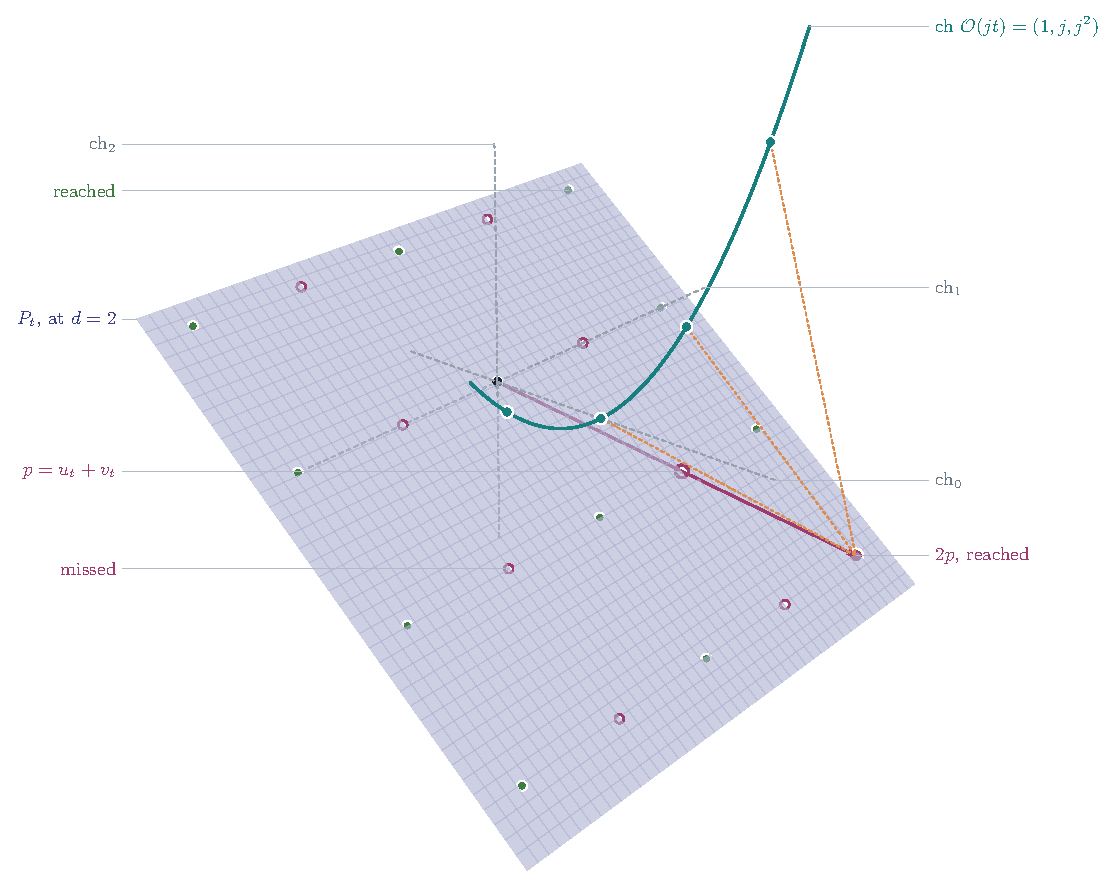
\includegraphics[width=0.86\textwidth]{fig_moment}
\caption{\Cref{thm:secantexists} at $n=2$ and $d=2$, in the coordinates
$(\ch_{0},\ch_{1},\ch_{2})$ of the basis $1$, $t$, $t^{2}/2$, the third axis at
two fifths scale. The characters of the powers of one line bundle lie on the
moment curve $j\mapsto(1,j,j^{2})$, and the Vandermonde determinant says that
any three of its points are affinely independent. The integral points of
$P_{t}=\QQ u_{t}\oplus\QQ v_{t}$ split by the criterion
$\ch_{2}\equiv\ch_{1}\bmod2$ into those the line bundles reach, drawn filled,
and those they miss, drawn open. Doubling $p=u_{t}+v_{t}$ lands on the
lattice, at the witness $-3[\cO_{X}]+8[\cO_{X}(t)]-3[\cO_{X}(2t)]$ of the
three dashed leaders.}
\label{fig:moment}
\end{figure}

\begin{remark}[What this closes, and what it does not]\label{rem:thirdclosed}
\Cref{thm:secantexists} settles the third of the four demands of
\Cref{q:higher}, for every $n\ge2$, every imaginary quadratic field and every
polarised abelian $n$-fold, and it does so with line bundles alone. Three
qualifications belong with it, and they are not small.

First, the theorem produces a sheaf and nothing more. It says nothing about
stability, about the rank being one, about the Ext groups, or about
semiregularity, and the construction of \Cref{lem:posrank} is not designed to
give any of them: the sheaf is assembled from line bundles and from quotients
supported on subvarieties, and its only controlled invariant is its class.
\Cref{prop:objectsize} applies to it as to any other object carrying the class,
and bounds $\sum_{i}\dim\Ext^{i}(\cF,\cF)$ from below.

This does not collide with \Cref{thm:positivity}, for the following reason. That
theorem concerns a perfect complex on the $2n$-fold $A$ whose Chern character
is an effective combination $\sum_{i}m_{i}e^{\lambda_{i}}$ with every $m_{i}$
positive, and it rules such a complex out because the norm form of $K$ is
positive definite. The class \eqref{eq:lbwitness} lives on the $n$-fold $X$,
not on $A$, and its coefficients alternate in sign; the witness at $n=4$ has
three negative ones. Positivity is exactly what is given up, and
\Cref{lem:posrank} is what replaces it, by requiring only that the total rank
be positive.

Second, the rank is large. \Cref{prop:genus3} at $n=3$ produces a rank one
sheaf, which is what Markman's argument uses and what \Cref{rem:markmancheck}
matches against the literature. The sheaf of \Cref{thm:secantexists} has rank
$Ma$, and $M$ grows quickly with $n$. Whether the rank can be brought down to
one at $n\ge4$, equivalently whether the lattice generated by the classes
$t^{k}/k!$ is realised by algebraic cycles on a general abelian $n$-fold rather
than only after clearing denominators, is a separate and open
question; on a Jacobian it is answered by the Abel--Jacobi cycles and
Poincar\'e's formula, and $M=1$ can be taken there.

Third, the fourth ingredient is untouched, and it is the one that matters. A
pair of secant sheaves gives a class on $X\times\widehat{X}$; making that class
remain of Hodge type across the moduli of polarised abelian $2n$-folds of Weil
type is a variational statement, and nothing here bears on it.
\Cref{rem:deformation} says what that step requires and stands unchanged.
We therefore do not claim the Hodge conjecture for abelian $2n$-folds of Weil
type at any $n\ge4$; what has changed is that three of the four ingredients of
\Cref{q:higher} are now theorems rather than questions.
\end{remark}

\subsection{What is supplied and what is not}

\begin{theorem}[Three of the four ingredients, in general]\label{thm:twoofthefour}
For every $n\ge2$, every squarefree $d>0$ and every polarised abelian $n$-fold
$X$ carrying a nondegenerate $\beta\in\NS(X)\otimes\QQ$, the data required by
\Cref{q:higher} exist and are explicit in the first three items:
\begin{enumerate}[label=\textup{(\alph*)}]
\item the abelian $2n$-fold of Weil type is $A=X\times\widehat{X}$ with the
  $K$-action \eqref{eq:Mdef}, by \Cref{thm:explicitweil};
\item the plane is $P_{t}$ of \Cref{def:secantplane} with $t=\beta$, it is
  spanned by Hodge classes and it meets the spinor variety in exactly the two
  conjugate points $[e^{\pm st}]$, by \Cref{thm:plane};
\item a pair of coherent sheaves $\cF_{1},\cF_{2}$ on $X$ whose Chern
  characters are linearly independent rational points of $P_{t}$ exists, by
  \Cref{thm:secantexists}, and each may be taken to have the class of an
  explicit integer combination of powers of one line bundle.
\end{enumerate}
The invariants of any such sheaf are forced by the explicit system of
\Cref{thm:secantinvariants}, which imposes $n-1$ linear conditions on a Chern
character already constrained to $\QQ[t]$, and are unobstructed numerically by
\eqref{eq:discnorm}.
\end{theorem}

\begin{proof}
(a), (b) and (c) are the cited theorems. For the count in the last sentence, a
Chern character in the subring $\QQ[t]\subset H^{\mathrm{ev}}(X,\QQ)$ is a
polynomial of degree at most $n$ in $t$, so lies in a space of dimension
$n+1$, while $P_{t}$ has dimension two.
\end{proof}

\begin{remark}[What is not supplied]\label{rem:deformation}
The fourth ingredient of \Cref{q:higher} is untouched by anything in this
section, and it is the hardest. Granting the pair of secant sheaves
$\cF_{1},\cF_{2}$ on $X$ that \Cref{thm:secantexists} now supplies, one must
still show that the characteristic class of
$\Phi(\cF_{1}^{\vee}\boxtimes\cF_{2})$ remains of Hodge type under every
deformation of $X\times\widehat{X}$ as a polarised abelian $2n$-fold of Weil
type, and that the object deforms with the variety, as a twisted sheaf to
first order. That step is carried out by Markman at $n=3$ \cite{Mar25b}, and it
rests on a semiregularity analysis. What we add to it is negative:
\Cref{thm:factor} identifies exactly which Hochschild classes the weakened
form of that analysis must kill for a secant object, and
\Cref{thm:candidatefails} shows that the only candidate proposed above
$n=3$ does not kill them. Without the step one obtains algebraicity only on
the split locus $X\times\widehat{X}$, where the Weil classes are of much
less interest, since the general abelian $2n$-fold of Weil type is simple and
is not of that form.

We therefore do not claim a proof of the Hodge conjecture for abelian
$2n$-folds of Weil type at any $n\ge4$, and nothing in this section should be
read as one. What we claim is that three of the four ingredients are now
written down for every $n$, the third of them with an explicit witness in
line bundles, and that the fourth is isolated.
\end{remark}

\begin{figure}[htbp]
\centering
  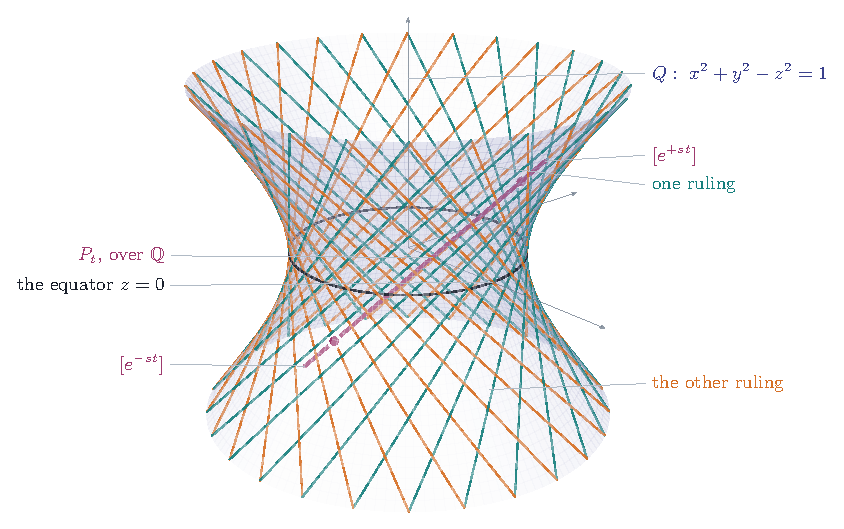
\includegraphics[width=0.88\textwidth]{fig_quadric}
\caption{The geometry of \Cref{thm:plane}, drawn in the smallest case in which
the even spinor variety is a surface, where it is a smooth quadric with its two
rulings. The line $P_{t}$ of \Cref{def:secantplane} is rational, and it meets
the variety in exactly the two points $[e^{\pm st}]$, which are conjugate over
$K$ and not individually rational. That is the configuration the Weil line
demands: a class defined over $\QQ$ cannot pick out one of the two points, so
the construction must carry the pair, and the pair spans a plane rather than a
line. \Cref{prop:orbitplane} is the same statement on the cohomological side,
and \Cref{fig:escape} places it among the hypotheses a construction can
satisfy.}
\label{fig:spinor}
\end{figure}

\subsection{The split member, in closed form}\label{ssec:split}

Before turning to what is missing, we record what the family gives outright.%
\footnote{The split locus is thin: a general abelian $2n$-fold of Weil type is simple, so it is not isogenous to a product at all, and the members $X\times\widehat{X}$ form a subvariety of $\cD_{n,n}$ of positive codimension. That is exactly why \Cref{cor:splitalgebraic} is a base case and not a solution, and why \Cref{q:residual} is about propagation.}
On the split member the Weil classes are not merely known to be algebraic;
they can be written down as polynomials in three divisor classes, and the
polynomial is the same for every $n$ and every $d$.

\begin{notation}\label{not:threeclasses}
On $A=X\times\widehat{X}$ write
\[
  \beta\in H^{2}(A,\QQ),
  \qquad
  \widehat{\beta}\in H^{2}(A,\QQ),
  \qquad
  \ell=c_{1}(\cP)\in H^{2}(A,\QQ)
\]
for the pullback of the polarisation of $X$, the pullback of the dual
polarisation of $\widehat{X}$, and the class of the Poincar\'e bundle. All
three are divisor classes, so every polynomial in them is algebraic. Put
\begin{equation}\label{eq:gammadef}
  \gamma=d\,\beta-\widehat{\beta}.
\end{equation}
\end{notation}

\begin{theorem}[The Weil line of the split member]\label{thm:splitclosed}
Let $A=X\times\widehat{X}$ carry the $K$-action \eqref{eq:Mdef} determined by a
principal $\beta$, and let $V_{\pm}\subset H^{1}(A,\CC)$ be the eigenspaces of
$\iota(\sqrt{-d})$. Then
\begin{enumerate}[label=\textup{(\roman*)},nosep]
\item $\gamma\mp\sqrt{-d}\,\ell$ lies in $\bigwedge^{2}V_{\pm}$, so it is an
  eigenclass for the character $\tau\mapsto\tau^{2}$ on $H^{2}(A,\CC)$
  respectively for its conjugate;
\item the generators of $\bigwedge^{2n}V_{\pm}$ are
  \begin{equation}\label{eq:splitclosed}
    \omega_{\pm}
    =\frac{(-1)^{n(n-1)/2}}{n!\,d^{\,n}}
      \bigl(\gamma\mp\sqrt{-d}\,\ell\bigr)^{n};
  \end{equation}
\item consequently the Weil line of $A$ is
  \[
    \HW(A)=\Bigl\langle\;
      \Re\bigl(\gamma-\sqrt{-d}\,\ell\bigr)^{n},\;\;
      \Im\bigl(\gamma-\sqrt{-d}\,\ell\bigr)^{n}
    \;\Bigr\rangle_{\QQ},
  \]
  and every Weil class on $A$ is a polynomial with rational coefficients in
  the three divisor classes $\beta,\widehat{\beta},\ell$, hence is algebraic.
\end{enumerate}
\end{theorem}

\begin{proof}
Write $U=H^{1}(X,\QQ)$ with basis $x_{1},\dots,x_{2n}$ chosen so that
$\beta=\sum_{j\le n}x_{j}\wedge x_{n+j}$, let $\xi_{1},\dots,\xi_{2n}$ be the
dual basis of $H^{1}(\widehat{X},\QQ)=U^{\vee}$, and let $B\colon U\to U^{\vee}$
be the isomorphism induced by $\beta$, so that $Bx_{j}=\xi_{n+j}$ and
$Bx_{n+j}=-\xi_{j}$. The endomorphism \eqref{eq:Mdef} acts on homology, and
its transpose acts on $H^{1}(A,\QQ)=U\oplus U^{\vee}$ by $u\mapsto -Bu$ and
$\phi\mapsto d\,B^{-1}\phi$;%
\footnote{In the basis $u_{1},\dots,u_{2n}$ of $H_{1}(X,\QQ)$ dual to the
$x_{i}$, the map $\beta\colon H_{1}(X)\to H^{1}(X)$ sends $u_{j}\mapsto
x_{n+j}$ and $u_{n+j}\mapsto-x_{j}$, so \eqref{eq:Mdef} sends
$u_{j}\mapsto dx_{n+j}$, $u_{n+j}\mapsto-dx_{j}$, $x_{n+j}\mapsto-u_{j}$ and
$x_{j}\mapsto u_{n+j}$; pairing with the dual basis gives the stated action
on $H^{1}(A,\QQ)$, where $\xi_{i}$ is the class dual to $x_{i}$ regarded as an
element of $H_{1}(\widehat X,\QQ)=H^{1}(X,\QQ)$.} its
square is $-d$; so, writing $\delta=\sqrt{-d}$,
\begin{equation}\label{eq:splitVpm}
  V_{\pm}=\Bigl\{\,u\pm\tfrac{\delta}{d}\,Bu\;:\;u\in U_{\CC}\Bigr\},
\end{equation}
since $M^{*}\bigl(u\pm\tfrac{\delta}{d}Bu\bigr)
=-Bu\pm\delta u=\pm\delta\bigl(u\pm\tfrac{\delta}{d}Bu\bigr)$.

(i) Take the sum over $j\le n$ of the wedges of the two eigenvectors attached
to $x_{j}$ and to $x_{n+j}$:
\[
  \sum_{j=1}^{n}
  \Bigl(x_{j}\pm\tfrac{\delta}{d}Bx_{j}\Bigr)\wedge
  \Bigl(x_{n+j}\pm\tfrac{\delta}{d}Bx_{n+j}\Bigr)
  =\beta\pm\tfrac{\delta}{d}\Sigma-\tfrac{1}{d}\widehat{\beta},
\]
using $\delta^{2}=-d$, where
$\Sigma=\sum_{j}\bigl(x_{j}\wedge Bx_{n+j}+Bx_{j}\wedge x_{n+j}\bigr)$ and
$\sum_{j}Bx_{j}\wedge Bx_{n+j}=\sum_{j}\xi_{n+j}\wedge(-\xi_{j})
=\widehat{\beta}$. Now
\[
  \Sigma=\sum_{j=1}^{n}\bigl(x_{j}\wedge(-\xi_{j})
        +\xi_{n+j}\wedge x_{n+j}\bigr)
   =-\sum_{i=1}^{2n}x_{i}\wedge\xi_{i}=-\ell .
\]
So the displayed sum is $\tfrac1d\bigl(d\beta-\widehat{\beta}\mp\delta\ell\bigr)
=\tfrac1d(\gamma\mp\delta\ell)$. It is a sum of wedges of pairs of vectors of
$V_{\pm}$, hence lies in $\bigwedge^{2}V_{\pm}$, which proves (i); the
statement about characters is \Cref{prop:grading} at $(r,s)=(2,0)$ and
$(0,2)$.

(ii) By (i) the $n$-th power $(\gamma\mp\delta\ell)^{n}$ lies in
$\bigwedge^{2n}V_{\pm}$, which is a line by \Cref{prop:weilline}. It is
nonzero: expanding $\gamma\mp\delta\ell=d\beta-\widehat{\beta}\mp\delta\ell$,
the only term of the $n$-th power lying in $\bigwedge^{2n}U$ is
$d^{\,n}\beta^{n}$, and $\beta^{n}\ne0$ because $\beta$ is nondegenerate;
the remaining terms all involve at least one $\xi$, so no cancellation can
occur. Hence $(\gamma\mp\delta\ell)^{n}$ spans $\bigwedge^{2n}V_{\pm}$ and is a
scalar multiple of $\omega_{\pm}=\bigwedge_{i=1}^{2n}\bigl(x_{i}\pm\tfrac{\delta}{d}Bx_{i}\bigr)$.
To find the scalar, compare the components in $\bigwedge^{2n}U$: that of
$\omega_{\pm}$ is $x_{1}\wedge\cdots\wedge x_{2n}$, while
\[
  d^{\,n}\beta^{n}=d^{\,n}\,n!\bigwedge_{j=1}^{n}(x_{j}\wedge x_{n+j})
  =d^{\,n}\,n!\,(-1)^{n(n-1)/2}\,x_{1}\wedge\cdots\wedge x_{2n},
\]
the sign being that of the permutation carrying
$(1,n+1,2,n+2,\dots,n,2n)$ to $(1,2,\dots,2n)$. Inverting gives
\eqref{eq:splitclosed}.

(iii) The two displayed classes are the real and imaginary parts of
$(\gamma-\delta\ell)^{n}$, which up to the nonzero rational factor in
\eqref{eq:splitclosed} are $\omega_{-}+\omega_{+}$ and
$(\omega_{-}-\omega_{+})/\delta$; by \Cref{prop:weilline}(i) these span
$\HW(A)$ over $\QQ$. Expanding $(\gamma-\delta\ell)^{n}$ by the binomial
theorem and separating even from odd powers of $\delta$ writes each of them as
a rational polynomial in $\beta,\widehat{\beta},\ell$, because
$\delta^{2m}=(-d)^{m}$ and $\delta^{2m+1}=(-d)^{m}\delta$. Products of divisor
classes are algebraic, so both are algebraic.
\end{proof}

\begin{example}\label{ex:splitsmall}
At $n=2$ the formula reads
\[
  \omega_{1}=d\,\ell^{2}-\gamma^{2},
  \qquad
  \omega_{2}=2\,\gamma\,\ell,
\]
and at $n=3$,
\[
  \omega_{1}=\gamma\,\ell^{2}-\tfrac13\gamma^{3},
  \qquad
  \omega_{2}=\gamma^{2}\ell-\tfrac13\,d\,\ell^{3},
\]
with $\gamma=d\beta-\widehat{\beta}$ throughout. Both cases, and the expansion
for every $n\le5$ and several $d$, are confirmed in
\texttt{split\_locus.py}; see item~(X) of \Cref{sec:verification}.
\end{example}

\begin{corollary}[Algebraicity on the split locus]\label{cor:splitalgebraic}
For every $n\ge1$, every squarefree $d>0$ and every principally polarised
abelian $n$-fold $X$, the Weil classes of $A=X\times\widehat{X}$ with the
$K$-action \eqref{eq:Mdef} are algebraic, and an algebraic representative is
given by \eqref{eq:splitclosed} as an explicit rational combination of
intersections of three divisors.
\end{corollary}

\begin{proof}
\Cref{thm:splitclosed}(iii), together with the Lefschetz theorem on $(1,1)$
classes, which makes $\beta,\widehat{\beta},\ell$ algebraic, and the fact that
the algebraic classes form a subring of $H^{*}(A,\QQ)$.
\end{proof}

\begin{remark}\label{rem:splitconsistent}
\Cref{cor:splitalgebraic} does not contradict \Cref{thm:character}. At the
split point $\NS(A)\otimes\QQ$ contains the three independent classes
$\beta,\widehat{\beta},\ell$, so the hypothesis
$\NS(A)\otimes\QQ=\QQ\eta$ of \Cref{prop:notpoly} fails, and this is the
situation of \Cref{rem:special}. What \Cref{thm:character} forbids is a
$\Kx$-eigenclass for the norm character meeting the Weil line, and
$\gamma\mp\sqrt{-d}\,\ell$ is an eigenclass for $\tau^{2}$ and for
$\bbar{\tau}^{2}$, not for the norm. Indeed \eqref{eq:splitclosed} is the
first place in this paper where a class in the right eigenspace is exhibited
at all, and it is exhibited only because the split member has enough divisors
to build one.
\end{remark}

\subsection{Products, and a base case in every dimension}\label{ssec:products}

The split member is one way to produce a member with enough divisors. There is
a second, and it behaves well under the one operation the Weil line respects.
Throughout this subsection $K$ is fixed and all Weil structures are for that
$K$.

\begin{lemma}[Products of Weil type]\label{lem:prodweil}
Let $(A_{1},\iota_{1},\eta_{1})$ be of $(K,-1,n_{1})$-Weil type and
$(A_{2},\iota_{2},\eta_{2})$ of $(K,-1,n_{2})$-Weil type. Then
$A=A_{1}\times A_{2}$, with the diagonal action
$\iota=\iota_{1}\times\iota_{2}$ and the product polarisation
$\eta=p_{1}^{*}\eta_{1}+p_{2}^{*}\eta_{2}$, is of
$(K,-1,n_{1}+n_{2})$-Weil type.
\end{lemma}

\begin{proof}
Write $V_{i}=H^{1}(A_{i},\QQ)$, so $V=H^{1}(A,\QQ)=V_{1}\oplus V_{2}$ as
$K$-vector spaces and $\dim_{K}V=2n_{1}+2n_{2}$. The Rosati involution of the
product polarisation is the product of the two Rosati involutions, so it
restricts on $K$ to conjugation, which is the sign $-1$ of
\Cref{def:weiltype}. For the multiplicities, the Hodge decomposition of $V$ is
the direct sum of those of $V_{1}$ and $V_{2}$, and the eigenspace
decomposition is likewise $V_{\pm}=V_{1,\pm}\oplus V_{2,\pm}$. Hence
\[
  \dim_{\CC}V_{+}^{1,0}
  =\dim_{\CC}V_{1,+}^{1,0}+\dim_{\CC}V_{2,+}^{1,0}
  =n_{1}+n_{2},
\]
and the same for the other three, which is \Cref{lem:balanced} for
$n=n_{1}+n_{2}$.
\end{proof}

The Weil line is the top exterior power over $K$, and a top exterior power of
a direct sum is the tensor product of the top exterior powers. That is the
whole content of the next theorem; what has to be checked is what it does to
the rational generators, since those are defined through the real structure
and not over $K$.

By \Cref{prop:weilline}(i) and (iii) the Weil line $\HW(A)$ is free of rank
one over $K$, and the basis $\omega_{1},\omega_{2}$ of
\Cref{thm:explicitgens} identifies $\HW(A)$ with $K$ itself by
$a\omega_{1}+b\omega_{2}\mapsto a+b\sqrt{-d}$. Write
$\omega(A)=\omega_{1}(A)+\sqrt{-d}\,\omega_{2}(A)$ for the resulting
$K$-valued invariant.

\begin{theorem}[The Weil class is multiplicative]\label{thm:weilmult}
With the notation of \Cref{lem:prodweil}, and cup product on
$H^{*}(A,\QQ)$ taken after pullback along the two projections,
\begin{equation}\label{eq:weilmult}
\begin{aligned}
  \omega_{1}(A)&=\tfrac12\bigl(\omega_{1}(A_{1})\,\omega_{1}(A_{2})
    -\omega_{2}(A_{1})\,\omega_{2}(A_{2})\bigr),\\
  \omega_{2}(A)&=\tfrac12\bigl(\omega_{1}(A_{1})\,\omega_{2}(A_{2})
    +\omega_{2}(A_{1})\,\omega_{1}(A_{2})\bigr),
\end{aligned}
\end{equation}
that is $\omega(A_{1})\,\omega(A_{2})=2\,\omega(A_{1}\times A_{2})$ in the
$K$-valued notation. For $k$ factors,
$\prod_{j}\omega(A_{j})=2^{k-1}\,\omega(A_{1}\times\cdots\times A_{k})$.
\end{theorem}

\begin{proof}
Let $\alpha_{\pm}^{i}$ generate $\bigwedge^{2n_{i}}V_{i,\pm}$. Since
$V_{\pm}=V_{1,\pm}\oplus V_{2,\pm}$,
\[
  \textstyle\bigwedge^{2n}V_{+}=\bigwedge^{2n_{1}}V_{1,+}\otimes
  \bigwedge^{2n_{2}}V_{2,+},
\]
so $\alpha_{+}=\alpha_{+}^{1}\wedge\alpha_{+}^{2}$ generates it, and likewise
$\alpha_{-}=\alpha_{-}^{1}\wedge\alpha_{-}^{2}$; the classes
$\alpha_{\pm}^{i}$ have even degree $2n_{i}$, so no sign enters when the two
blocks of generators are interleaved. By
\Cref{thm:explicitgens}(iii), $\omega_{1}=\alpha_{+}+\alpha_{-}$ and
$\omega_{2}=\sqrt{-d}\,(\alpha_{+}-\alpha_{-})/(-d)$ up to the normalisation
fixed there, so it suffices to expand. Writing $\omega_{1}^{i}$ and
$\omega_{2}^{i}$ for the generators of the factors,
\[
  \omega_{1}^{1}\omega_{1}^{2}-\omega_{2}^{1}\omega_{2}^{2}
  =(\alpha_{+}^{1}+\alpha_{-}^{1})(\alpha_{+}^{2}+\alpha_{-}^{2})
  +(\alpha_{+}^{1}-\alpha_{-}^{1})(\alpha_{+}^{2}-\alpha_{-}^{2})
  =2(\alpha_{+}^{1}\alpha_{+}^{2}+\alpha_{-}^{1}\alpha_{-}^{2})
  =2\,\omega_{1}(A),
\]
the cross terms cancelling in pairs, and the same computation with one factor
conjugated gives the second identity of \eqref{eq:weilmult}. In the $K$-valued
notation the two identities together say
$\omega(A_{1})\omega(A_{2})=2\omega(A)$, since the map
$a\omega_{1}+b\omega_{2}\mapsto a+b\sqrt{-d}$ carries the right-hand sides of
\eqref{eq:weilmult} to the real and imaginary parts of the product. The
statement for $k$ factors follows by induction, each application contributing
one factor of $2$. The identities are verified in exact arithmetic over
$\QQ(\sqrt{-d})$ for all $n_{1},n_{2}\le3$ and for the four-factor products
listed in \Cref{sec:verification}, item (XV).
\end{proof}

\begin{corollary}[Algebraicity propagates along products]\label{cor:prodalg}
If the Weil classes of $A_{1}$ and of $A_{2}$ are algebraic, then so are those
of $A_{1}\times A_{2}$, and an algebraic representative is the rational
combination of external products given by \eqref{eq:weilmult}.
\end{corollary}

\begin{proof}
Algebraic classes are closed under pullback along the projections and under
cup product, and \eqref{eq:weilmult} expresses $\omega_{1}(A)$ and
$\omega_{2}(A)$ in those operations applied to the $\omega_{j}(A_{i})$.
\end{proof}

The base case costs nothing.

\begin{lemma}[Dimension two]\label{lem:basecase}
Let $A_{0}$ be of $(K,-1,1)$-Weil type, so $\dim A_{0}=2$. Then
$\HW(A_{0})\subset H^{2}(A_{0},\QQ)$ and both generators are algebraic.
\end{lemma}

\begin{proof}
The Weil classes lie in $H^{2n}=H^{2}$ and are of type $(1,1)$ by
\Cref{prop:weilline}(ii), so they are algebraic by the Lefschetz theorem on
$(1,1)$ classes. No hypothesis on $A_{0}$ beyond the Weil structure is used.
\end{proof}

\begin{theorem}[An algebraic Weil class in every dimension]\label{thm:everyn}
Let $n\ge1$, let $d>0$ be squarefree, and let $A_{1},\dots,A_{n}$ be abelian
surfaces of $(K,-1,1)$-Weil type. Then $A=A_{1}\times\cdots\times A_{n}$ is of
$(K,-1,n)$-Weil type and its Weil classes are algebraic; explicitly, by
\Cref{thm:weilmult} and \Cref{lem:basecase} they are
$2^{-(n-1)}$ times the real and imaginary parts of
$\prod_{j=1}^{n}\bigl(\omega_{1}(A_{j})+\sqrt{-d}\,\omega_{2}(A_{j})\bigr)$,
a polynomial with integer coefficients in $2n$ divisor classes.
\end{theorem}

\begin{proof}
\Cref{lem:prodweil} gives the Weil structure, \Cref{lem:basecase} gives
algebraicity of each factor's classes, and \Cref{cor:prodalg} applied $n-1$
times gives the conclusion; the displayed form is \Cref{thm:weilmult} for $k=n$
factors. Each $\omega_{j}(A_{i})$ is a divisor class by
\Cref{lem:basecase}, so the product is a polynomial in $2n$ of them.
\end{proof}

\begin{remark}[What this locus is, and what it is not]\label{rem:prodscope}
\Cref{thm:everyn} is unconditional and holds at every $n$, and it is the only
statement in this paper that produces an algebraic Weil class in every
dimension without quoting anything. It should not be mistaken for more than it
is. The family of polarised abelian $2n$-folds of $(K,-1,n)$-Weil type has
dimension $n^{2}$, and the locus of products of $n$ surfaces has dimension
$n$, so for $n\ge2$ it is a proper closed subvariety, and a smaller one than
the quaternionic locus of \Cref{thm:quatweil}, whose dimension is
$n(n+1)/2$. A general member of the family is simple, so it is not isogenous
to a product at all, and neither \Cref{thm:everyn} nor
\Cref{cor:splitalgebraic} touches it. What the product construction adds is a
second family of base points, defined for every $n$ and every $d$, at which the
class is not merely known to be algebraic but is written down; and it adds the
observation that the algebraicity locus is closed under the product operation,
so that any future case $n_{0}$ propagates to every multiple of $n_{0}$ and to
every sum of solved cases. Combined with Markman's theorem at $n=2$
\cite{Mar25a,Mar25b} this gives, at every $n$, algebraicity on the locus of
products of abelian fourfolds and surfaces of Weil type, of dimension $2n$ when
$n$ is even. The general member remains outside every one of these loci, and
by \Cref{thm:residual} the gap between them and the general member is exactly
the propagation statement that this paper does not prove.
\end{remark}

\begin{figure}[htbp]
\centering
  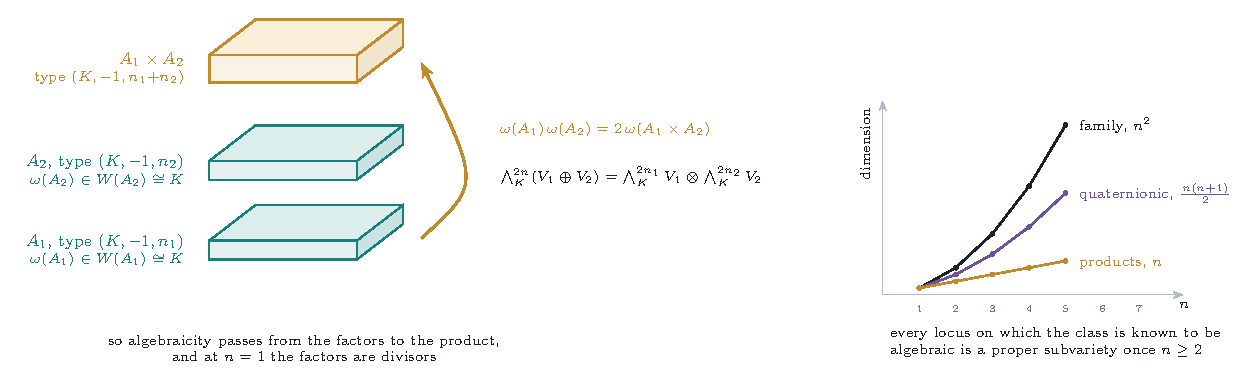
\includegraphics[width=0.96\textwidth]{fig_product}
\caption{\Cref{thm:weilmult} and its reach. Left: the Weil line of each factor
is a $K$-line, the Weil line of the product is the tensor product of the two
over $K$, and in the $K$-valued notation the class is multiplicative up to the
factor $2$. Algebraicity therefore passes from the factors to the product, and
at $n=1$ the factors are divisor classes, so a product of $n$ abelian surfaces
of Weil type carries an explicit algebraic Weil class in every dimension.
Right: the dimensions of the loci on which the class is known to be algebraic,
against the dimension $n^{2}$ of the family. Both the quaternionic locus and
the product locus are proper subvarieties once $n\ge2$, and a general member
lies on neither.}
\label{fig:product}
\end{figure}

\subsection{The residual statement}\label{ssec:residual}

Everything above lets the remaining question be stated in one sentence with no
auxiliary hypotheses, and we state it, because a problem in that form is
worth more than a programme.

\begin{setupenv}[The family]\label{setup:family}
Fix $n\ge2$ and a squarefree $d>0$. Let $\cD_{n,n}$ be the period domain of
\Cref{prop:weildomain} and let
\[
  \pi\colon\cA\longrightarrow\cD_{n,n}
\]
be the family of polarised abelian $2n$-folds of $(K,-1,n)$-Weil type it
parametrises, with $\omega$ the flat section of $R^{2n}\pi_{*}\QQ$ given
fibrewise by the class $\omega_{1}$ of \eqref{eq:omegagens}. Let
$\cD^{\mathrm{spl}}\subset\cD_{n,n}$ be the locus of split members
$X\times\widehat{X}$ carrying the action \eqref{eq:Mdef}.
\end{setupenv}

\begin{question}[The residual statement]\label{q:residual}
Is $\omega_{s}$ algebraic for every $s\in\cD_{n,n}$?
\end{question}

\begin{theorem}[The reduction]\label{thm:residual}
Fix $n\ge2$ and a squarefree $d>0$, and keep the notation of
\Cref{setup:family}.
\begin{enumerate}[label=\textup{(\alph*)},nosep]
\item If \Cref{q:residual} has a positive answer, then the Hodge conjecture
  holds, in every degree, for every abelian $2n$-fold of $(K,-1,n)$-Weil type
  with $\Hg(A)=\SU(V,H)$.
\item Conversely, if the Hodge conjecture holds for every abelian $2n$-fold of
  $(K,-1,n)$-Weil type, then \Cref{q:residual} has a positive answer.
\item $\cD^{\mathrm{spl}}$ is nonempty, $\omega_{s}$ is algebraic at every
  $s\in\cD^{\mathrm{spl}}$ with the explicit representative
  \eqref{eq:splitclosed}, and $\cD_{n,n}$ is connected.
\end{enumerate}
So \Cref{q:residual} is the variational Hodge conjecture for one flat class on
one connected family, it is necessary as well as sufficient, and its base case
is supplied. \Cref{thm:everyfamily} supplies one in every family, for every
discriminant, so the hypothesis of nonemptiness is never the obstacle.
\end{theorem}

\begin{proof}
(a) Let $A$ be of $(K,-1,n)$-Weil type with $\Hg(A)=\SU(V,H)$. By
\Cref{prop:weildomain} its Hodge structure is a point $s$ of $\cD_{n,n}$, so
$A$ is a fibre of $\pi$, and the Weil line of $A$ is generated over $K$ by
$\omega_{s}$. A positive answer makes $\omega_{s}$ algebraic, hence makes the
whole Weil line algebraic by the argument of \Cref{cor:whatisleft}, and by
\Cref{thm:hdgcount} the Weil line together with the powers of $\eta$ exhausts
$\Hdg^{*}(A)$.

(b) For every $s$ the class $\omega_{s}$ is a Hodge class on the fibre $A_{s}$,
by \Cref{prop:weilline}(ii), and $A_{s}$ is of $(K,-1,n)$-Weil type by
construction. So the Hodge conjecture for $A_{s}$ gives its algebraicity.

(c) $\cD^{\mathrm{spl}}$ is nonempty because the construction \eqref{eq:Mdef}
applies to any principally polarised abelian $n$-fold and produces a point of
$\cD_{n,n}$ by \Cref{thm:explicitweil}; algebraicity there is
\Cref{cor:splitalgebraic}; and $\cD_{n,n}$ is connected because it is a
bounded symmetric domain, by \Cref{prop:weildomain}.
\end{proof}

\begin{remark}[Why this is the precise target]\label{rem:target}
Three things have been removed from the problem by the preceding sections, and
we list what is left after each.

\Cref{thm:hdgcount} removes the question of how many classes are at issue:
one, in one degree, on each fibre. \Cref{thm:divisor} and
\Cref{thm:character} remove two families of would-be constructions, so no
effort need be spent on them. \Cref{thm:splitclosed} removes the base case: the
class is algebraic somewhere in the family, with a representative one can
write on a single line.

What is left is propagation, and it is exactly Grothendieck's variational
Hodge conjecture for the pair $(\pi,\omega)$ of \Cref{setup:family}. That
statement is open in general; what \Cref{thm:residual} adds is that for the
Hodge conjecture on abelian varieties of Weil type it is not merely sufficient
but necessary, so no other route can avoid an equivalent difficulty.
\Cref{ssec:properness} takes the propagation apart. The passage from a formal
deformation to an algebraic one, which is usually the awkward half, is
supplied there by properness of the Hilbert scheme, and what survives is the
infinitesimal half at a single point, or else a bound on the size of the
cycles already constructed.
\end{remark}

\subsection{The divisorial criterion, and exactly what it reaches}
\label{ssec:divcrit}

\Cref{thm:splitclosed} is a computation on one member of the family. The
mechanism behind it is not special to that member, and isolating the mechanism
turns the base case into a criterion that can be tested at any point. The
criterion, and the precise determination of where it holds, is the content of
this subsection.

\begin{theorem}[The divisorial criterion]\label{thm:divcriterion}
Let $(A,\iota,\eta)$ be of $(K,-1,n)$-Weil type and suppose there exists
$\Theta\in\bigwedge^{2}V_{-}$ with
\begin{enumerate}[label=\textup{(\roman*)},nosep]
\item $\Theta$ nondegenerate as an alternating form on $V_{-}^{\vee}$,
  equivalently $\Theta^{n}\ne0$;
\item $\Theta$ of Hodge type $(1,1)$;
\item $\Theta+\bbar{\Theta}$ rational, that is in $H^{2}(A,\QQ)$.
\end{enumerate}
Then the Weil classes of $A$ are algebraic. Explicitly, writing
$g=\Theta+\bbar{\Theta}$ and $\lambda=(\Theta-\bbar{\Theta})/\sqrt{-d}$, both
$g$ and $\lambda$ are divisor classes and
\begin{equation}\label{eq:divrep}
  \HW(A)=\Bigl\langle\;
    \Re\bigl(g+\sqrt{-d}\,\lambda\bigr)^{n},\;\;
    \Im\bigl(g+\sqrt{-d}\,\lambda\bigr)^{n}\;\Bigr\rangle_{\QQ},
\end{equation}
so every Weil class is a rational polynomial in two divisor classes.
\end{theorem}

\begin{proof}
Conjugation interchanges $\bigwedge^{2}V_{-}$ and $\bigwedge^{2}V_{+}$, so
$\bbar{\Theta}\in\bigwedge^{2}V_{+}$, and both $g$ and $\lambda$ are fixed by
conjugation, hence real. Rationality of $g$ is (iii); rationality of
$\lambda$ needs an argument, and it is the following. Fix
$\tau=a+b\sqrt{-d}\in\Kx$ with $ab\ne0$. By \Cref{prop:grading} the operator
$\iota(\tau)^{*}$ acts on $\bigwedge^{2}V_{+}$ by $\tau^{2}=a^{2}-db^{2}+2ab\sqrt{-d}$
and on $\bigwedge^{2}V_{-}$ by $\bbar{\tau}^{\,2}$, so
\[
  J:=\frac{\iota(\tau)^{*}-(a^{2}-db^{2})}{2ab}
\]
is a $\QQ$-rational endomorphism of $H^{2}(A,\QQ)$ preserving $R$ and acting
on $\bigwedge^{2}V_{\pm}$ by $\pm\sqrt{-d}$. Applying it to
$g=\Theta+\bbar{\Theta}$ gives $J(g)=-\sqrt{-d}\,\Theta+\sqrt{-d}\,\bbar{\Theta}
=-\sqrt{-d}\cdot\sqrt{-d}\,\lambda=d\,\lambda$, so $\lambda=J(g)/d$ is
rational. Both $g$ and $\lambda$ are of type $(1,1)$ by (ii) and conjugation
symmetry, so both lie in $\NS(A)\otimes\QQ$ by the Lefschetz theorem on
$(1,1)$ classes, and both are algebraic.

By (i) the form $\Theta$ on the $2n$-dimensional space $V_{-}$ has nonzero
Pfaffian, so $\Theta^{n}$ is a nonzero element of the line
$\bigwedge^{2n}V_{-}$, and it therefore spans it; conjugating,
$\bbar{\Theta}^{\,n}$ spans $\bigwedge^{2n}V_{+}$. Hence
$\Theta^{n}+\bbar{\Theta}^{\,n}$ and
$(\Theta^{n}-\bbar{\Theta}^{\,n})/\sqrt{-d}$ span $\HW(A)$ over $\QQ$, by
\Cref{prop:weilline}(i). Finally
$2^{n}\Theta^{n}=(g+\sqrt{-d}\lambda)^{n}$, and expanding by the binomial
theorem with $(\sqrt{-d})^{2m}=(-d)^{m}$ writes the real and imaginary parts
as rational polynomials in $g$ and $\lambda$. Products of divisor classes are
algebraic.
\end{proof}

\begin{corollary}\label{cor:splitsatisfies}
The split member of \Cref{thm:splitclosed} satisfies the criterion, with
$\Theta=\gamma-\sqrt{-d}\,\ell$ and $\gamma=d\beta-\widehat{\beta}$; the two
divisor classes of \eqref{eq:divrep} are $2\gamma$ and $-2\ell$.
\end{corollary}

\begin{proof}
\Cref{thm:splitclosed}(i) gives $\Theta\in\bigwedge^{2}V_{+}$ for the sign
$\gamma-\sqrt{-d}\ell$, and the conjugate lies in $\bigwedge^{2}V_{-}$;
$\gamma$ and $\ell$ are divisor classes, hence of type $(1,1)$, so $\Theta$ is
of type $(1,1)$ and $\Theta+\bbar{\Theta}=2\gamma$ is rational.
Nondegeneracy is the nonvanishing of $\Theta^{n}$, proved in
\Cref{thm:splitclosed}(ii).
\end{proof}

So the base case is one instance of a general criterion. The next two results
say exactly how far the criterion reaches, and both are negative in a way that
is worth knowing.

\begin{proposition}[The criterion fails at a general point]\label{prop:divfails}
Let $(A,\iota,\eta)$ be of $(K,-1,n)$-Weil type with $n\ge2$ and
$\Hg(A)=\SU(V,H)$. Put
\[
  R=\Bigl(\textstyle\bigwedge^{2}V_{+}\oplus\bigwedge^{2}V_{-}\Bigr)
      \cap H^{2}(A,\QQ).
\]
Then $R\cap\NS(A)_{\QQ}=0$, and no $\Theta$ as in \Cref{thm:divcriterion}
exists.
\end{proposition}

\begin{proof}
By \Cref{prop:normpart} the space $R$ is a rational sub-Hodge structure of
$H^{2}(A,\QQ)$ admitting no proper nonzero rational sub-Hodge structure, and
by \Cref{prop:h2pieces} it has $h^{2,0}=2\binom{n}{2}=n(n-1)$, which is
positive for $n\ge2$. The intersection
$R\cap\NS(A)_{\QQ}$ is a rational sub-Hodge structure of $R$, so it is $0$ or
all of $R$; it is of pure type $(1,1)$, and $R$ is not, so it is $0$. A
$\Theta$ as in \Cref{thm:divcriterion} would give the nonzero element
$\Theta+\bbar{\Theta}$ of $R\cap\NS(A)_{\QQ}$.
\end{proof}

\begin{proposition}[What the split locus is]\label{prop:splitgeom}
Fix $n\ge1$ and a squarefree $d>0$, and let $A=X\times\widehat{X}$ carry the
$K$-action \eqref{eq:Mdef} determined by a nondegenerate
$\beta\in\NS(X)\otimes\QQ$ of elementary divisors $(d_{1},\dots,d_{n})$.
\begin{enumerate}[label=\textup{(\roman*)},nosep]
\item Let $B$ be the Gram matrix of $\beta$ in a basis of $U$, and let
  $\widehat\beta$ be the form on $U^{\vee}$ with Gram matrix $-B^{-1}$ in the
  dual basis, which for principal $\beta$ is the class of
  \Cref{not:threeclasses}. The polarisation of $A$ is
  $\eta=\beta+\widehat{\beta}/d$, a positive rational multiple of
  $d\beta+\widehat\beta$; its Gram matrix on $H_{1}(A,\QQ)=U\oplus U^{\vee}$
  is the block form $Q=B\oplus(-B^{-1}/d)$, and $M$ is anti-self-adjoint for
  it.
\item In the $K$-basis $u_{1},\dots,u_{2n}$ of $H_{1}(A,\QQ)$ the hermitian
  form of \Cref{lem:hermform} has Gram matrix $\sqrt{-d}\,B$, so
  \[
    \det H=(-d)^{n}\det B=(-d)^{n}(d_{1}\cdots d_{n})^{2},
  \]
  and $(-1)^{n}\det H=d^{\,n}(d_{1}\cdots d_{n})^{2}$ is a norm from $K$.
  Every split member therefore lies in the Weil family of trivial
  discriminant, whatever $\beta$ is chosen.
\item The split members form a locus of dimension $n(n+1)/2$ inside
  $\cD_{n,n}$, of codimension $n(n-1)/2$, which is zero only for $n=1$ and is
  a divisor for $n=2$.
\item For $X$ with $\Hg(X)=\mathrm{Sp}(H^{1}(X,\QQ))$ one has
  $\NS(A)_{\QQ}=\langle\beta,\widehat{\beta},\ell\rangle$, of rank three, and
  in degree $2n$ the monomials in those three classes span the whole space of
  Hodge classes of $A$.
\end{enumerate}
\end{proposition}

\begin{proof}
(i) In the chosen basis of $U$ and the dual basis of $U^{\vee}$ the map
$\beta\colon U\to U^{\vee}$ has matrix $B^{\top}=-B$ and its inverse has
matrix $-B^{-1}$, so \eqref{eq:Mdef} becomes
$M=\begin{psmallmatrix}0&B^{-1}\\-dB&0\end{psmallmatrix}$, with
$M^{2}=-d$ and
$M^{\top}=\begin{psmallmatrix}0&dB\\-B^{-1}&0\end{psmallmatrix}$, using
$B^{\top}=-B$ and $(B^{-1})^{\top}=-B^{-1}$. For a block form
$Q=\begin{psmallmatrix}P&\Lambda\\-\Lambda^{\top}&S\end{psmallmatrix}$ the
Rosati relation $M^{\top}Q+QM=0$ reads
$B\Lambda^{\top}+\Lambda B=0$, $dBS+PB^{-1}=0$, $B^{-1}P+dSB=0$ and
$B^{-1}\Lambda+\Lambda^{\top}B^{-1}=0$. Taking $\Lambda=0$ and $P=B$ forces
$S=-B^{-1}/d$ from the second relation, and the third then reads $-I+I=0$.
So $Q=B\oplus(-B^{-1}/d)$, which is the Gram matrix of
$\beta+\widehat\beta/d$. For principal $\beta$ one may take
$B=\begin{psmallmatrix}0&I\\-I&0\end{psmallmatrix}$, so that $-B^{-1}=B$
and $\widehat\beta=\sum_{j}\xi_{j}\wedge\xi_{n+j}$ as in
\Cref{not:threeclasses}. The computation is repeated entry by entry for
$n\le4$ in item (XI) of \Cref{sec:verification}, together with the check
that the induced action on $H^{2}(A,\QQ)$ multiplies $d\beta+\widehat\beta$
by $d$ and $\gamma$, $\ell$ by $-d$, and that $\beta+d\widehat\beta$ is not
an eigenclass when $d>1$.

(ii) The set $u_{1},\dots,u_{2n}$ is a $K$-basis because
$MU=d\beta(U)=U^{\vee}$, and $H(u_{i},u_{j})=Q(Mu_{i},u_{j})+\sqrt{-d}\,Q(u_{i},u_{j})$
by \eqref{eq:QfromH}; the first term vanishes since $Mu_{i}\in U^{\vee}$,
$u_{j}\in U$ and $Q$ has no cross block by (i), and the second is
$\sqrt{-d}\,\beta_{ij}$. Hence the Gram matrix is $\sqrt{-d}\,B$ and
$\det H=(\sqrt{-d})^{2n}\det B=(-d)^{n}\det B$. The determinant of an
alternating matrix is the square of its Pfaffian, here $(d_{1}\cdots
d_{n})^{2}$. Now $d=\Nm_{K/\QQ}(\sqrt{-d})$ is a norm and every square is a
norm, and the norms form a subgroup of $\QQ^{\times}$, so
$d^{\,n}(d_{1}\cdots d_{n})^{2}$ is a norm.

(iii) A split member is determined by $X$ together with $\beta$, and the
polarised moduli of $X$ has dimension $\dim\cA_{n}=n(n+1)/2$ while the type of
$\beta$ is discrete. By \Cref{prop:weildomain} the ambient domain has
dimension $n^{2}$, and $n^{2}-n(n+1)/2=n(n-1)/2$.

(iv) The Hodge classes of $A=X\times\widehat{X}$ are the invariants of
$\Hg(A)=\Hg(X)=\mathrm{Sp}(U)$ acting on
$\bigwedge^{*}(U\oplus U^{\vee})$. In degree two the invariants are the three
lines spanned by $\beta$, $\widehat{\beta}$ and $\ell$, one from each Kunneth
summand $\bigwedge^{2}U$, $U\otimes U^{\vee}$ and $\bigwedge^{2}U^{\vee}$.
In degree $2n$ the dimension of the invariant space is computed from the
primitive decomposition $\bigwedge^{a}U=\bigoplus_{j}\bigwedge^{a-2j}_{0}U$
together with Schur's lemma, and it agrees with the rank of the set of
monomials $\beta^{i}\widehat{\beta}^{j}\ell^{k}$ with $i+j+k=n$; both numbers
are computed for $n\le3$ in item (XI) of \Cref{sec:verification} and agree.
\end{proof}

\begin{remark}[Where this leaves the residual statement]\label{rem:residualmap}
Putting \Cref{prop:splitgeom}(ii) beside \Cref{thm:residual} changes the shape
of what is left. The Weil families for a fixed $K$ and fixed $n$ are
classified by the discriminant of the hermitian form, an element of
$\QQ^{\times}_{>0}/\Nm_{K/\QQ}(K^{\times})$, which is an infinite group. The
split construction of \Cref{ssec:split} produces a base point in exactly one of
them, the one with trivial discriminant; products of abelian surfaces of Weil
type (\Cref{thm:everyn}, \Cref{lem:products}) reach every discriminant, but
only on a locus of dimension $n$. So \Cref{q:residual} is really two
questions, and they are of different kinds.
\begin{enumerate}[label=\textup{(R\arabic*)},leftmargin=2.8em,itemsep=2pt]
\item \emph{Trivial discriminant.} A base point exists, with the explicit
  cycle \eqref{eq:splitclosed}, and what is missing is propagation off a locus
  of codimension $n(n-1)/2$. At $n=2$ that locus is a divisor and the
  propagation is known, by Markman \cite{Mar25a,Mar25b} and by Floccari and Fu
  \cite{FF26}; combined with \Cref{thm:residual}(a) this recovers the Hodge
  conjecture for abelian fourfolds of Weil type of trivial discriminant with
  full Hodge group. At $n=3$ it is settled as well, by Markman's theorem on
  the sixfolds of trivial discriminant \cite{Mar25a,Mar25b}, for every $K$.
  For $n\ge4$ it is open, and by \Cref{prop:descent} it is then the only
  question left in the imaginary quadratic case.
\item \emph{Nontrivial discriminant.} The construction of this subsection
  never lands there, by \Cref{prop:splitgeom}(ii), so it supplies no base
  point; and by \Cref{prop:divfails} no divisorial argument can supply one at
  a general member. A base point must come from a special member at which $R$
  acquires Hodge classes.
\end{enumerate}
Question (R2) is settled in \Cref{ssec:everyfamily}: the special members
required are those with quaternionic multiplication extending $K$, they exist
in every family, and on them \Cref{thm:divcriterion} applies. After that only
(R1) remains, now with a base point in every family.
\end{remark}

\begin{remark}[The split locus is larger than a Hodge locus has to be]
\label{rem:nlcodim}
A component of the Noether--Lefschetz locus of a weight two variation has
codimension at most $h^{2,0}$, here $n(n-1)$. The split locus has codimension
$n(n-1)/2$ by \Cref{prop:splitgeom}(iii), exactly half of that, so it is a
component of twice the expected dimension. That is a reflection of
\Cref{prop:splitgeom}(iv): at a split point $R$ acquires two independent Hodge
classes at once, namely $\gamma$ and $\ell$, and each of them costs
$h^{2,0}/2$ conditions rather than $h^{2,0}$. Whether there are components of
the expected codimension carrying only one class, and whether the criterion of
\Cref{thm:divcriterion} can be met on them, is the concrete form of question
(R2).
\end{remark}

\subsection{A base point in every family}\label{ssec:everyfamily}

\Cref{prop:splitgeom}(ii) says the split construction reaches one discriminant
class. \Cref{thm:divcriterion} does not care where its $\Theta$ comes from,
and the source used below is an endomorphism rather than a pair of divisors
chosen by hand. It reaches every class, and with it question (R2) of
\Cref{rem:residualmap} is settled.

\begin{definition}[Discriminant]\label{def:disc}
For $(A,\iota,\eta)$ of $(K,-1,n)$-Weil type with hermitian form $H$ as in
\Cref{lem:hermform}, the \emph{discriminant} is the class of
$(-1)^{n}\det H$ in $\QQ^{\times}_{>0}/\Nm_{K/\QQ}(K^{\times})$. The sign
makes the representative positive, because $H$ has signature $(n,n)$; and the
class is well defined because changing the $K$-basis multiplies $\det H$ by a
norm. Hermitian forms of rank $2n$ over $K$ with signature $(n,n)$ are
classified by this class, so it labels the Weil families.
\end{definition}

The mechanism behind \Cref{thm:divcriterion} can be named. A class in $R$ is
the same thing as an endomorphism that conjugates $K$.

\begin{lemma}[What a class in $R$ is]\label{lem:Rendomorphism}
Let $(A,\iota,\eta)$ be of $(K,-1,n)$-Weil type. The map $\mu\mapsto
g_{\mu}$, $g_{\mu}(x,y)=\eta(\mu x,y)$, is a bijection between
\begin{enumerate}[label=\textup{(\alph*)},nosep]
\item the elements $\mu\in\End^{0}(A)$ with $\mu^{\dagger}=\mu$ and
  $\mu\,\iota(\tau)=\iota(\bbar{\tau})\,\mu$ for all $\tau\in K$, and
\item the elements of $R\cap\NS(A)_{\QQ}$.
\end{enumerate}
Under it, $\mu$ invertible corresponds to $g_{\mu}$ nondegenerate, hence to a
nondegenerate $\Theta$. If such a $\mu\ne0$ exists and the centraliser of
$\iota(K)$ in $\End^{0}(A)$ is $\iota(K)$, then $\mu^{2}\in\QQ^{\times}$ and
$\iota(K)+\iota(K)\mu$ is a quaternion algebra $(-d,\mu^{2})_{\QQ}$ inside
$\End^{0}(A)$.
\end{lemma}

\begin{proof}
A class in $\NS(A)_{\QQ}$ is a symmetric homomorphism $A\to\Av$ up to isogeny,
that is $\eta\mu$ with $\mu^{\dagger}=\mu$. The condition
$g_{\mu}(\iota(\tau)x,y)=g_{\mu}(x,\iota(\tau)y)$, which says that $g_{\mu}$ is
$K$-bilinear and hence lies in $R=\bigwedge^{2}_{K}V$, reads
$\eta(\mu\iota(\tau)x,y)=\eta(\mu x,\iota(\tau)y)=\eta(\iota(\tau)^{\dagger}\mu
x,y)=\eta(\iota(\bbar{\tau})\mu x,y)$, using \Cref{def:weiltype}(iii); so it is
exactly $\mu\iota(\tau)=\iota(\bbar{\tau})\mu$. For the last sentence,
$\mu^{2}$ commutes with $\iota(K)$, hence lies in $\iota(K)$ by hypothesis, and
$\mu\mu^{2}\mu^{-1}=\mu^{2}$ forces it to be fixed by conjugation, so
$\mu^{2}\in\QQ^{\times}$. Then $\iota(\sqrt{-d})$ and $\mu$ generate the
quaternion algebra with the stated invariants.
\end{proof}

So the criterion asks for quaternionic multiplication extending $K$. Such
abelian varieties exist in abundance, and their invariants can be computed.

\begin{setupenv}[The quaternionic model]\label{setup:quat}
Let $b\in\QQ_{>0}$ and let $B=(-d,b)_{\QQ}$ be the quaternion algebra with
basis $1,i,j,ij$ and $i^{2}=-d$, $j^{2}=b$, $ij=-ji$. Let
$V=B^{n}$ as a left $B$-module, of dimension $4n$ over $\QQ$, let
$K=\QQ(i)\subset B$ act through $i$, and fix $a_{1},\dots,a_{n}\in\QQ^{\times}$
and
\begin{equation}\label{eq:quatE}
  E(x,y)=\sum_{k=1}^{n}a_{k}\,\mathrm{trd}\bigl(\bbar{x_{k}}\,i\,y_{k}\bigr),
\end{equation}
where $\mathrm{trd}$ is the reduced trace and $\bbar{\phantom{x}}$ the
canonical involution of $B$.
\end{setupenv}

\begin{theorem}[Weil type from quaternionic multiplication]\label{thm:quatweil}
With the data of \Cref{setup:quat}:
\begin{enumerate}[label=\textup{(\roman*)},nosep]
\item $E$ is alternating and nondegenerate, and its Rosati involution is
  $\beta\mapsto i^{-1}\bbar{\beta}i$, which restricts to complex conjugation on
  $K$ and fixes $j$; it is positive, the form $\mathrm{trd}(\beta\beta^{\dagger})$
  being diagonal with entries $2,2d,2b,2db$ on the basis;
\item in the $K$-basis $e_{1},e_{1}j,\dots,e_{n},e_{n}j$ of $V$ the hermitian
  form of \Cref{lem:hermform} is
  \[
    H=\mathrm{diag}\bigl(2a_{1}d,\,-2a_{1}bd,\;\dots,\;2a_{n}d,\,-2a_{n}bd\bigr),
  \]
  of signature $(n,n)$;
\item there is a complex structure on $V_{\RR}$ commuting with $B$ and
  polarised by $E$, and for every such the resulting abelian variety $A$ is of
  $(K,-1,n)$-Weil type, the balanced signature being forced and not imposed;
\item the discriminant of $A$ is the class of $b^{n}$;
\item $\mu=$ left multiplication by $j$ satisfies \Cref{lem:Rendomorphism}(a),
  so $g=g_{\mu}$ lies in $R\cap\NS(A)_{\QQ}$ and is nondegenerate, the
  divisorial criterion \Cref{thm:divcriterion} applies, and the Weil classes
  of $A$ are algebraic.
\end{enumerate}
\end{theorem}

\begin{proof}
(i) $\mathrm{trd}(z)=\mathrm{trd}(\bbar{z})$ and
$\overline{\bbar{x}iy}=\bbar{y}\,\bbar{i}\,x=-\bbar{y}ix$ give
$E(y,x)=-E(x,y)$. Nondegeneracy is the nondegeneracy of the reduced trace
pairing. For the Rosati, $E(\beta x,y)=E(x,\beta^{\dagger}y)$ for all $x,y$
reads $\bbar{\beta}i=i\beta^{\dagger}$, that is
$\beta^{\dagger}=i^{-1}\bbar{\beta}i$. Then $i^{\dagger}=-i$ and, since
$(-j)i=ij$, also $j^{\dagger}=i^{-1}(ij)=j$. Positivity is the displayed
diagonal, which is positive because $d>0$ and $b>0$.

(ii) $V=Ke_{k}\oplus Ke_{k}j$ over all $k$, since $B=K\oplus Kj$. By
\eqref{eq:QfromH}, $H(x,y)=E(ix,y)+\sqrt{-d}\,E(x,y)$. On one factor,
$E(ix,y)=a\,\mathrm{trd}(\overline{ix}\,i\,y)=-a\,\mathrm{trd}(\bbar{x}i^{2}y)
=ad\,\mathrm{trd}(\bbar{x}y)$, so
\[
  H(x,y)=a\bigl[d\,\mathrm{trd}(\bbar{x}y)+\sqrt{-d}\,\mathrm{trd}(\bbar{x}iy)\bigr].
\]
Now $\mathrm{trd}(1)=2$, $\mathrm{trd}(i)=\mathrm{trd}(j)=\mathrm{trd}(ij)=0$,
$\bbar{j}j=-b$ and $\bbar{j}ij=ib$, which give $H(1,1)=2ad$,
$H(j,j)=-2abd$ and $H(1,j)=0$. Since $b>0$ the two entries of each block have
opposite signs, so the signature is $(n,n)$.

(iii) A complex structure commuting with $B$ and compatible with $E$ is the
same as a subspace $V^{1,0}\subset V_{\CC}$, stable under $B$, with
$V_{\CC}=V^{1,0}\oplus\overline{V^{1,0}}$ and the two Riemann relations. Being
$K$-stable it splits as $P\oplus P'$ with $P\subset V_{+}$ and
$P'\subset V_{-}$; left multiplication by $j$ is $\sigma$-semilinear, so it
carries $V_{+}$ to $V_{-}$, and $B$-stability forces $P'=jP$. Conversely, for
any $n$-dimensional $H$-negative definite $P\subset V_{+}$ the subspace
$P\oplus jP$ is $B$-stable and satisfies the Riemann relations, by the
computation in the proof of \Cref{thm:model} applied blockwise; such $P$
exists because $H$ has signature $(n,n)$ by (ii). Since $j$ is invertible and
carries $P$ isomorphically to $P'$, one gets $\dim P=\dim P'=n$, which is
\Cref{def:weiltype}(ii). The general theory of abelian varieties with
prescribed endomorphism structure is in \cite[Ch.~9]{BL04}.

(iv) By (ii), $\det H=\prod_{k}(2a_{k}d)(-2a_{k}bd)=(-1)^{n}b^{n}\bigl(2^{n}d^{n}
\prod_{k}a_{k}\bigr)^{2}$, so $(-1)^{n}\det H$ is $b^{n}$ times a square, and
squares are norms.

(v) Left multiplication by $j$ satisfies $\mu^{\dagger}=\mu$ by (i) and
$\mu\,\iota(\tau)=\iota(\bbar{\tau})\,\mu$ because $ji=-ij$; it is invertible
because $\mu^{2}=b\ne0$. \Cref{lem:Rendomorphism} puts $g_{\mu}$ in
$R\cap\NS(A)_{\QQ}$ and makes it nondegenerate, and
\Cref{thm:divcriterion} applies to the component $\Theta$ of $g_{\mu}$ in
$\bigwedge^{2}V_{-}$.
\end{proof}

\begin{proposition}[Nothing numerical forbids the object]%
\label{prop:notforbidden}
Let $t$ be a principal polarisation on $X$ and let
$\ch=au+bv$ be a rational point of the secant plane of \Cref{thm:plane},
with $a,b\in\ZZ$. Then
\begin{enumerate}[label=\textup{(\roman*)},nosep]
\item every $\ch_{k}$ is an integral multiple of the integral class
  $t^{k}/k!$, the multiple being $\pm a d^{j}$ in even degree $k=2j$ and
  $\pm b d^{j}$ in odd degree $k=2j+1$;
\item the Chern classes $c_{1},\dots,c_{n}$ obtained from $\ch$ by Newton's
  identities are integral, for every $n\le8$, every squarefree $d\le11$ and
  every $a\le4$, $|b|\le4$;
\item the discriminant is
  $\Delta=2rc_{2}-(r-1)c_{1}^{2}=\bigl(a^{2}d+b^{2}\bigr)t^{2}
  =\Nm_{K/\QQ}(b+a\sqrt{-d})\,t^{2}$, which is positive, so Bogomolov's
  inequality never binds.
\end{enumerate}
\end{proposition}

\begin{proof}
(i) is the definition of $u$ and $v$: the coefficient of $t^{k}$ is
$a(-d)^{j}/(2j)!$ or $b(-d)^{j}/(2j+1)!$, and multiplying by $k!$ clears the
factorial and leaves $\pm ad^{j}$ or $\pm bd^{j}$. For (ii), Newton's
identities express $k!\,c_{k}$ as an integer polynomial in the $i!\,\ch_{i}$
apart from one division by $k$ at each step, and the computation in item (XX)
of \Cref{sec:verification} carries out those divisions exactly over the stated
range and finds them exact every time. (iii) is the computation recorded in
\Cref{thm:secantinvariants}, and the norm form of an imaginary quadratic field
is positive definite.
\end{proof}

\begin{remark}[What this settles, and what it does not]%
\label{rem:notforbidden}
The content is negative and that is the point. One might hope that the object
the construction needs at $n\ge4$ is forbidden by its numbers, in which case
the secant route would be dead on arithmetic alone and the residual question
would change shape. \Cref{prop:notforbidden} says it is not: the invariants
are integral, the discriminant is positive, and nothing in Riemann--Roch or in
Bogomolov's inequality stands in the way. Taken with \Cref{prop:objectsize},
which bounds the size of the object from below without forbidding it, and with
the parameter count of \Cref{rem:markmancheck}, which fixes the rank one shape
at $n=3$, the position is that every count we know how to
make is consistent with the object existing and none of them produces it. What
is missing at $n\ge4$ is the object, not a number.
\end{remark}

\subsection{The quaternionic locus is a Lagrangian Grassmannian}
\label{ssec:lagrangian}

\Cref{thm:quatweil} produces a point of the family for each admissible
$\psi$, and the footnote to \Cref{rem:ntwo} records the dimension of the
locus of all such points by a Morita argument. The locus is more than a
dimension, and saying what it is puts the residual difficulty in one line.

\begin{proposition}[The quaternionic locus]\label{prop:lagrangian}
Keep \Cref{setup:quat} and let $\psi$ be $K$-semilinear, invertible,
Rosati-symmetric, with $\psi^{2}=b$. For $x,y\in V_{+}$ put
\[
  \omega_{\psi}(x,y)\;=\;E(x,\psi y).
\]
\begin{enumerate}[label=\textup{(\roman*)},nosep]
\item $\omega_{\psi}$ is a nondegenerate alternating form on $V_{+}$, and it
  is alternating precisely because $\psi$ is Rosati-symmetric.
\item A point $P=V_{+}^{1,0}$ of $\cD_{n,n}$ lies on the locus where $\psi$
  is a morphism of Hodge structures if and only if $P$ is isotropic for
  $\omega_{\psi}$.
\item Since $\dim_{\CC}V_{+}=2n$ and $\dim_{\CC}P=n$, such a $P$ is
  Lagrangian, so the locus is the open subset of
  $\mathrm{LG}(n,V_{+},\omega_{\psi})$ cut out by negative definiteness of
  $H$. Its dimension is $n(n+1)/2$ and its codimension in $\cD_{n,n}$ is
  $n(n-1)/2$.
\end{enumerate}
\end{proposition}

\begin{proof}
(i) $\psi$ carries $V_{+}$ to $V_{-}$, since it is semilinear, and $E$ pairs
$V_{+}$ with $V_{-}$ perfectly, so $\omega_{\psi}$ is defined and
nondegenerate. Rosati symmetry is the identity $E(\psi x,y)=E(x,\psi y)$;
with $E$ alternating it gives
$\omega_{\psi}(y,x)=E(y,\psi x)=E(\psi x,y)\cdot(-1)=-\omega_{\psi}(x,y)$.

(ii) Suppose $\psi$ preserves the Hodge structure. Being semilinear it
carries $V_{+}^{1,0}$ into $V_{-}^{1,0}$, so $\psi P\subseteq V^{1,0}$, and
$E$ vanishes on $V^{1,0}$ by the first Riemann relation; hence
$E(P,\psi P)=0$, which is the isotropy of $P$. Conversely, if $P$ is
isotropic then $\psi P$ lies in the $E$-annihilator of $P$ inside $V_{-}$.
That annihilator has dimension $n$, because $E$ pairs $V_{+}$ with $V_{-}$
perfectly, and it contains $V_{-}^{1,0}$, which also has dimension $n$ and is
$E$-orthogonal to $P$ since both lie in $V^{1,0}$. The two therefore agree,
so $\psi P=V_{-}^{1,0}$ and $\psi$ preserves $V^{1,0}$.

(iii) A Lagrangian Grassmannian $\mathrm{LG}(n,2n)$ has dimension $n(n+1)/2$,
its tangent space at a Lagrangian $P$ being the symmetric forms on $P$;
negative definiteness is an open condition and does not change the dimension.
Subtracting from $\dim\cD_{n,n}=n^{2}$ gives $n(n-1)/2$. The chart by
symmetric forms, the isotropy of its members, and the two dimensions are
checked for $n\le5$ in item (XVII) of \Cref{sec:verification}.
\end{proof}

\begin{figure}[htbp]
\centering
  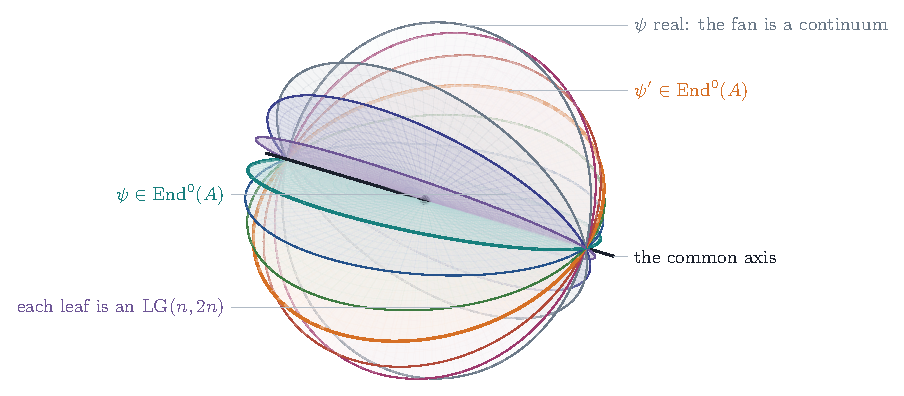
\includegraphics[width=0.80\textwidth]{fig_lagsweep}
\caption{\Cref{prop:lagrangian}, drawn as a pencil. Each admissible $\psi$ gives
one leaf, an open piece of $\mathrm{LG}(n,V_{+},\omega_{\psi})$ of dimension
$n(n+1)/2$, and the leaves through a common axis form a continuous family as
$\psi$ varies over the reals, so they sweep $\cD_{n,n}$. The two drawn heavy
are the ones whose $\psi$ is rational, and only those are quaternionic loci of
an actual abelian variety. The picture is exact for the pencil it draws; in
the family the leaves have dimension $n(n+1)/2$ inside $n^{2}$ and the
parameter is not one real number but a variety of them. \protect\footnotemark}
\label{fig:lagsweep}
\end{figure}
\footnotetext{Drawing the leaves as planes through one axis is faithful to the feature
that matters, that the family is continuous and its rational members are not.
It is not faithful to the codimension, which is $n(n-1)/2$ and therefore zero
only at $n=1$; at $n=2$ the leaves are divisors, which is \Cref{rem:ntwo}.}

\begin{remark}[What this says about the residual difficulty]%
\label{rem:onlyrational}
The description is worth having because of what it makes visible. Fix a
point $P$ of $\cD_{n,n}$. Complete a basis of $P$ to a basis of $V_{+}$ and
let $\omega$ be the alternating form that is standard in that basis; then $P$
is Lagrangian for $\omega$, and $\omega$ is $\omega_{\psi}$ for a real
$\psi$ satisfying every condition of \Cref{prop:lagrangian} except
rationality. So the quaternionic loci, taken over the \emph{real} $\psi$,
cover $\cD_{n,n}$ completely; they cover it with room to spare, since each
has dimension $n(n+1)/2$ and they are parametrised by a positive dimensional
family. What stops the covering is that $\psi$ must lie in
$\End^{0}(A)$, hence be rational, and the rational $\psi$ form a countable
set.

That is \Cref{cor:allornothing} again, with everything else stripped away. It
is not a deformation-theoretic difficulty and not a positivity difficulty;
it is a countable set of parameters inside an uncountable one. We state it in
this form because it is the sharpest version we can give of what a new idea
would have to supply: a mechanism that moves the Lagrangian Grassmannians
continuously, or equivalently that produces from one rational $\psi$ a family
of cycles over a neighbourhood rather than over its own locus, is the whole
of \Cref{q:residual}.
\end{remark}

\begin{lemma}[Products]\label{lem:products}
Let $(A_{1},\iota_{1},\eta_{1})$ and $(A_{2},\iota_{2},\eta_{2})$ be of
$(K,-1,n_{1})$- and $(K,-1,n_{2})$-Weil type. Then
$A_{1}\times A_{2}$ with the diagonal $K$-action and the product polarisation
is of $(K,-1,n_{1}+n_{2})$-Weil type, its hermitian form is the orthogonal
sum, its discriminant is the product of the two discriminants, and if both
factors satisfy the divisorial criterion then so does the product.
\end{lemma}

\begin{proof}
Signatures and hermitian forms add over an orthogonal sum, so the signature is
$(n_{1}+n_{2},n_{1}+n_{2})$ and $\det H=\det H_{1}\det H_{2}$, whence
$(-1)^{n_{1}+n_{2}}\det H$ is the product of the two normalised determinants.
For the criterion, $V_{-}=V_{1,-}\oplus V_{2,-}$, and
$\Theta=\Theta_{1}+\Theta_{2}$ lies in $\bigwedge^{2}V_{-}$, is of type
$(1,1)$, has $\Theta+\bbar{\Theta}$ rational, and is nondegenerate on the
direct sum because each summand is nondegenerate on its factor.
\end{proof}

\begin{theorem}[A base point in every Weil family]\label{thm:everyfamily}
Let $K=\QQ(\sqrt{-d})$, let $n\ge1$, and let $\delta$ be any class in
$\QQ^{\times}_{>0}/\Nm_{K/\QQ}(K^{\times})$. Then there is an abelian
$2n$-fold $A$ of $(K,-1,n)$-Weil type with discriminant $\delta$ whose Weil
classes are algebraic, with an explicit representative as a rational
polynomial in two divisor classes.
\end{theorem}

\begin{proof}
Choose $b\in\QQ_{>0}$ representing $\delta$.

If $n$ is odd, take the quaternionic model of \Cref{setup:quat} with this $b$.
Its discriminant is $b^{n}=b\cdot(b^{(n-1)/2})^{2}$, which is $\delta$, and
its Weil classes are algebraic by \Cref{thm:quatweil}(v).

If $n$ is even, take $A=A_{1}\times A_{2}$ with $A_{1}$ the quaternionic model
at $n_{1}=1$ and parameter $b$, and $A_{2}$ the quaternionic model at
$n_{2}=n-1$ and parameter $d$. Both factors satisfy the criterion, so the
product does by \Cref{lem:products}; and the discriminant is
$b^{1}\cdot d^{\,n-1}$, which is $\delta$ because $d=\Nm_{K/\QQ}(\sqrt{-d})$ is
a norm. The dimension is $2(1+(n-1))=2n$.

In both cases the representative is \eqref{eq:divrep} for the class
$g_{\mu}$ of \Cref{thm:quatweil}(v), or the sum of the two such classes.
\end{proof}

\begin{corollary}[Question (R2) is settled]\label{cor:R2}
Every Weil family contains a member at which the Weil classes are algebraic.
Consequently \Cref{q:residual} reduces to propagation alone: the Hodge
conjecture for abelian $2n$-folds of Weil type, for every $n$ and every
discriminant, holds if and only if the class $\omega$ of
\Cref{setup:family} propagates from the nonempty locus where it is known to be
algebraic to the rest of its connected family.
\end{corollary}

\begin{proof}
The first sentence is \Cref{thm:everyfamily} applied to each class, together
with the fact that the families are indexed by those classes
(\Cref{def:disc}). The second is \Cref{thm:residual} with the base locus now
known to be nonempty in every family.
\end{proof}

\begin{remark}[What is left, and what it is not]\label{rem:whatsleftnow}
The residual statement is now a single one. It is the variational Hodge
conjecture for one flat class on one connected family, with a base point
supplied in every family, and by \Cref{thm:residual} it is necessary as well
as sufficient. Two features of it are worth recording, because they say which
tools cannot settle it.

The base locus is thin. By \Cref{prop:divfails} the divisorial criterion fails
at every point with full Hodge group, so the locus where it holds is contained
in the Noether--Lefschetz locus of $R$, a countable union of proper closed
algebraic subvarieties of $\cD_{n,n}$ by \Cref{thm:cdk}. Enlarging the base
locus further by the same method is therefore impossible; any new point it
produces is again special.

The propagation is not formal. By \Cref{rem:variational} the infinitesimal
form of it would follow from semiregularity of the cycle at a base point, and
the cycle at a base point is now explicit in every family, being an
intersection of two divisors raised to the $n$-th power. Whether it is
semiregular is a computation in the normal bundle that we have not carried
out. The second half of that objection, that a positive answer would give
deformation only in the formal category, is answered in
\Cref{ssec:properness}: once the algebraic locus is known to be a countable
union of closed subvarieties, a formal deformation at one point is enough.
\end{remark}

\subsection{The exact form of what remains}\label{ssec:exactform}

The algebraicity of a Hodge class is usually approached through an
intermediate property. A rational class of type $(p,p)$ is \emph{absolutely
Hodge} if, after spreading the variety out over a finitely generated field and
applying any automorphism of $\CC$, the de Rham component of the class remains
of type $(p,p)$ in every comparison. The implications

\begin{equation}\label{eq:threechain}
  \text{algebraic}
  \;\Longrightarrow\;
  \text{absolutely Hodge}
  \;\Longrightarrow\;
  \text{Hodge}
\end{equation}
are both elementary; the Hodge conjecture is the reverse of the first, and the
reverse of the second is the weaker question that Deligne settled for abelian
varieties.

\begin{theorem}[Deligne \cite{Del82}]\label{thm:deligneAH}
Every Hodge class on a complex abelian variety is absolutely Hodge. Moreover,
\emph{Principle B}: if $\pi\colon\cX\to S$ is smooth projective over a
connected smooth base, and $\alpha$ is a flat section of $R^{2p}\pi_{*}\QQ(p)$
that is Hodge at every point of $S$ and absolutely Hodge at one point, then it
is absolutely Hodge at every point.
\end{theorem}

Put beside \Cref{thm:residual} and \Cref{thm:everyfamily}, this locates the
remaining problem precisely, and the location is worth stating because it is
not where one might guess.

\begin{corollary}[What is left, in one implication]\label{cor:exactform}
Let $\pi\colon\cA\to\cD_{n,n}$ and $\omega$ be as in \Cref{setup:family}. Then
$\omega_{s}$ is absolutely Hodge for every $s$, and the following are
equivalent:
\begin{enumerate}[label=\textup{(\roman*)},nosep]
\item the Hodge conjecture holds, in every degree, for every abelian
  $2n$-fold of $(K,-1,n)$-Weil type with $\Hg(A)=\SU(V,H)$;
\item the absolutely Hodge class $\omega_{s}$ is algebraic for every $s$.
\end{enumerate}
This holds for every $K$, every $n$ and every discriminant.
\end{corollary}

\begin{proof}
The first assertion is \Cref{thm:deligneAH}; alternatively, and this is the
point of the present section, it follows from Principle B together with
\Cref{thm:everyfamily}, which supplies a point of $\cD_{n,n}$ at which
$\omega$ is algebraic and hence absolutely Hodge, and with the connectedness of
$\cD_{n,n}$ from \Cref{prop:weildomain}. The equivalence is
\Cref{thm:residual}(a) and (b).
\end{proof}

\begin{remark}[Why the remaining implication resists the methods used here]
\label{rem:whyterminal}
The two halves of \eqref{eq:threechain} behave differently in families, and
the difference is the whole of the difficulty.

Principle B holds because being absolutely Hodge is a condition one can test
after spreading out over a finitely generated field, the set of Hodge classes
of bounded norm is finite by \Cref{lem:boundednorm}, and the locus where a
class stays Hodge is algebraic by \Cref{thm:cdk}; those three facts let one
propagate the property along $S$. Being algebraic has no counterpart of the
first: a cycle class is not determined by finitely many numerical conditions
that a field automorphism preserves, and the group of cycles is not locally
constant in a family. That is exactly the content of the variational Hodge
conjecture, and nothing in this paper supplies it.

An obstruction of this shape is removed in one of three ways: by a correspondence that carries the problem to a variety where
the class is a divisor or an endomorphism, which is what Kuga and Satake do
for weight two and what \Cref{cor:ksboundary} shows is unavailable here beyond
$n=1$; by a construction that produces the cycle directly at the general
point, which \Cref{thm:divisor} and \Cref{thm:character} close for two natural
families of constructions and \Cref{prop:divfails} closes for every divisorial
one; or by turning the statement over the whole family into a statement at one
point, which is what \Cref{ssec:properness} does.

The last of those is as far as we get. \Cref{thm:degreebound} and
\Cref{thm:semiregclosure} each reduce \Cref{cor:exactform}(ii), in its
entirety, to a property of the cycles already constructed in
\Cref{ssec:everyfamily}: a bound on their size along one orbit, or the
injectivity of one linear map attached to one of them. Neither reduction
appeals to a general point, to a limit, or to an unproved conjecture. We have
not established either property, so we do not claim the Hodge conjecture; what
we claim is that after \Cref{rem:tworemain} the outstanding question is of a
different kind from the one \Cref{q:residual} began with.
\end{remark}

\subsection{The algebraic locus is closed, and what that costs}
\label{ssec:properness}

Everything so far has been pointwise: a class at a point, a criterion at a
point, a cycle at a point, and in \Cref{cor:exactform} an implication to be
proved at every point. The propagation question of \Cref{q:residual} is about
the set
\[
  \Sigma \;=\; \bigl\{\,s\in\cD_{n,n} \;:\;
    \omega_{s}\ \text{is algebraic on}\ A_{s}\,\bigr\},
\]
and nothing has yet been said about what kind of set that is. It turns out to
be a very restricted kind, and the restriction changes the shape of the
remaining problem: instead of a class to construct at every point, one is left
with a bound to prove along one orbit, or a rank to compute at one point.
The mechanism is that the Hilbert scheme is proper, so each piece of $\Sigma$
cut out by bounded data is Zariski closed.\footnote{The mechanism is not new.
That the locus where a fixed Hodge class becomes algebraic is a countable
union of closed subvarieties is the standard companion to the statement that
the Hodge locus itself is a countable union of closed subvarieties, for which
see \cite[Chapter~5]{Voi03} and, in the form we use in \Cref{thm:cdk},
\cite{CDK95}. What is specific to the present situation is that the class
whose algebraic locus is being described has been pinned down completely by
\Cref{thm:hdgcount} and written out by \Cref{thm:explicitgens}, that the locus
is known to be nonempty in every family by \Cref{thm:everyfamily}, and that
the group acting has been identified. Those three inputs are what turn a soft
statement into a criterion one can try to verify.}

\begin{setupenv}[The quotient, and the universal family]\label{setup:shimura}
Keep \Cref{setup:family}. Fix an integer $N\ge3$ and let $\Gamma$ be the
subgroup of $\SU(V,H)(\QQ)$ preserving the lattice $L\subset V$ used to build
the family and acting trivially on $L/NL$. Write
\[
  p\colon\cD_{n,n}\longrightarrow\cS=\Gamma\backslash\cD_{n,n} .
\]
By Baily and Borel \cite{BB66} the quotient $\cS$ is a smooth quasi-projective
complex variety, and it is irreducible because $\cD_{n,n}$ is connected. Since
$N\ge3$ the level structure rigidifies, so $\cS$ carries a universal family
\[
  f\colon\cA\longrightarrow\cS,
\]
and the relative polarisation $3\eta$ is relatively very ample, which fixes a
relative projective embedding and hence a notion of degree in the fibres.
Write $G=\SU(V,H)$, an algebraic group over $\QQ$, so that
$G(\RR)$ acts transitively on $\cD_{n,n}$ and $\Gamma\subset G(\QQ)$.
\end{setupenv}

Two small facts have to be recorded before the main one, because both are used
without comment later and neither is quite automatic.

\begin{lemma}[The section descends]\label{lem:omegadescends}
The section $\omega$ of \Cref{setup:family} is $\Gamma$-invariant, hence
descends to a flat section of $R^{2n}f_{*}\QQ$ over $\cS$ that is of type
$(n,n)$ at every point.
\end{lemma}

\begin{proof}
The Weil line is $\HW=\bigwedge^{2n}_{K}V$, and an element of $\SU(V,H)$ is by
definition a $K$-linear automorphism of $V$ of $K$-determinant $1$. Its action
on the top $K$-exterior power is multiplication by that determinant, so
$\Gamma$ acts trivially on $\HW$ and in particular fixes $\omega$. Flatness is
then immediate, and the Hodge type at every point is
\Cref{prop:weilline}(ii).
\end{proof}

\begin{lemma}[One component is enough]\label{lem:onecomponent}
Let $(A,\iota,\eta)$ be of $(K,-1,n)$-Weil type with
$\iota(\cO_{K})\subseteq\End(A)$, and let $\HW\subset H^{2n}(A,\QQ)$ be its
Weil line. If one nonzero element of $\HW$ is algebraic, every element of
$\HW$ is algebraic.\footnote{This is the step compressed into the last
sentence of the proof of \Cref{cor:whatisleft}, written out because the
witness $\tau$ has to be chosen and because the choice is the same one the
Lean theorem \texttt{irrational\_witness\_exists} certifies. The determinant
that makes the two classes independent is $b(w_{1}^{2}+dw_{2}^{2})$ for
$\tau^{2n}=a+b\sqrt{-d}$ and $w=w_{1}+w_{2}\sqrt{-d}$, and that is the content
of \texttt{weil\_line\_spanned}.}
\end{lemma}

\begin{proof}
Among the elements $\tau_{m}=m+\sqrt{-d}$ of $\cO_{K}$ with $1\le m\le7$ the
ratios $\tau_{m}/\bbar{\tau}_{m}$ are pairwise distinct, since
$\tau_{m}\bbar{\tau}_{m'}$ is rational only when $m=m'$. The group of roots of
unity in an imaginary quadratic field has order $2$, $4$ or $6$, so some $m$
in that range has $\tau=\tau_{m}$ with $\tau/\bbar\tau$ not a root of unity,
and then $\tau^{2n}\ne\bbar{\tau}^{2n}$, that is $\tau^{2n}\notin\QQ$, for
every $n\ge1$.\footnote{The exceptional witnesses are real and are the reason
the argument names a range rather than taking $m=1$: for $d=1$ the ratio
attached to $1+\sqrt{-1}$ is a primitive fourth root of unity and for $d=3$
the ratio attached to $1+\sqrt{-3}$ is a primitive sixth root of unity, so at
those two values of $d$ the naive witness fails for the divisible $n$. The
Lean theorems \texttt{bad\_witness} and \texttt{bad\_witness\_exceptions} of
\Cref{sec:lean} record exactly which pairs fail and that no others do in the
range searched.}

Since $\tau\in\cO_{K}$, the element $\iota(\tau)$ is an endomorphism of $A$,
so $\iota(\tau)^{*}$ on $H^{2n}(A,\QQ)$ is induced by the graph
correspondence and therefore carries algebraic classes to algebraic classes.
On $H^{1}$ it is multiplication by $\tau$, so on
$\bigwedge^{2n}_{K}V$ it is multiplication by $\tau^{2n}$. As
$\tau^{2n}\notin\QQ$ and $\HW$ is a one dimensional $K$-vector space, the pair
$w,\;\tau^{2n}w$ is a $\QQ$-basis of $\HW$ for every $w\ne0$. If $w$ is
algebraic then so is $\iota(\tau)^{*}w=\tau^{2n}w$, and the two together span.
\end{proof}

\begin{theorem}[The algebraic locus is a countable union of closed
subvarieties]\label{thm:closedlocus}
Keep \Cref{setup:shimura}. For a finite tuple $\underline{P}=(P_{1},\dots
,P_{m})$ of Hilbert polynomials and a tuple $\underline{q}\in\QQ^{m}$ put
\begin{align*}
  \cH_{\underline{P}}
  &\;=\;
  \Hilb^{P_{1}}(\cA/\cS)\times_{\cS}\cdots\times_{\cS}\Hilb^{P_{m}}(\cA/\cS),
  \\[2pt]
  \Sigma_{\underline{P},\underline{q}}
  &\;=\;
  \mathrm{pr}\Bigl(\bigl\{\,\underline{Z}\in\cH_{\underline{P}}
    \;:\;\textstyle\sum_{i}q_{i}[Z_{i}]=\omega\,\bigr\}\Bigr)
  \;\subseteq\;\cS .
\end{align*}
Then each $\Sigma_{\underline{P},\underline{q}}$ is Zariski closed in
$\cS$,\footnote{The bound on the Hilbert polynomials is what the statement
lives on, and it cannot be dropped. Without it one is looking at the image of
an infinite disjoint union, and an infinite union of closed sets need be
neither closed nor constructible; indeed the whole difficulty of the Hodge
conjecture in families is that $\Sigma$ itself is not known to be either. The
relative Chow variety of effective $n$-cycles of bounded degree would serve
equally well in place of the Hilbert schemes, with the same proof, and the
choice between them is immaterial here because all that is used is properness
over the base together with the local constancy of the cycle class. What is
used later, and what forces the bookkeeping with tuples rather than a single
subscheme, is that a rational cycle is a rational combination of several
integral ones and the several may have different Hilbert polynomials.} and
\[
  p^{-1}\Bigl(\,\bigcup_{\underline{P},\underline{q}}
    \Sigma_{\underline{P},\underline{q}}\Bigr)\;=\;\Sigma ,
\]
the union running over a countable index set.
\end{theorem}

\begin{proof}
Each $\Hilb^{P_{i}}(\cA/\cS)$ is projective over $\cS$ by Grothendieck's
existence theorem \cite{Gro61}, so the fibre product $\cH_{\underline{P}}$ is
projective over $\cS$, and being of finite type it has finitely many connected
components.

Fix a connected component $T$, replace it by its reduction, which changes
neither the underlying space nor any cohomology group, and let
$\cZ_{i}\subset\cA\times_{\cS}T$ be the pullback of the $i$-th universal
subscheme. It is flat over $T$ and its fibres have Hilbert polynomial $P_{i}$
of degree $n$, so the associated $n$-cycles, the top-dimensional components
counted with their multiplicities, are the fibres of a cycle on
$\cA\times_{\cS}T$ whose class restricts on the fibre over $t$ to $[Z_{i,t}]$.
Restriction of a global class to the fibres of a topologically
locally trivial family is a flat section of the local system, so
$t\mapsto\sum_{i}q_{i}[Z_{i,t}]$ is flat on $T$; and $\omega$ is flat on $\cS$
by \Cref{lem:omegadescends}, hence flat after pullback. Two flat sections of a
local system over a connected base agree everywhere as soon as they agree at
one point, so the locus where they agree is a union of connected components of
$\cH_{\underline{P}}$. That locus is therefore itself projective over $\cS$,
and the image of a proper morphism is Zariski closed.

For the equality of sets, let $s\in\cS$ with $\omega_{s}$ algebraic. Then
$\omega_{s}=\sum_{i}q_{i}[Z_{i}]$ for finitely many closed integral subschemes
$Z_{i}\subset A_{s}$ of dimension $n$ and rationals $q_{i}$; taking
$P_{i}$ to be the Hilbert polynomial of $Z_{i}$ puts $s$ in
$\Sigma_{\underline{P},\underline{q}}$. The converse holds because the class
of a closed subscheme of pure dimension $n$ is algebraic. Countability is
clear: a Hilbert polynomial is determined by its finitely many integer
coordinates in the binomial basis, and $\QQ$ is countable.
\end{proof}

\begin{corollary}[All, or almost nothing]\label{cor:allornothing}
Exactly one of the following holds.
\begin{enumerate}[label=\textup{(\alph*)},nosep]
\item $\Sigma=\cD_{n,n}$, and the Hodge conjecture holds in every degree for
  every abelian $2n$-fold of $(K,-1,n)$-Weil type with $\Hg(A)=\SU(V,H)$ in
  the family.
\item $\Sigma$ has empty interior in the analytic topology. Its complement is
  then a dense $G_{\delta}$, so $\omega_{s}$ fails to be algebraic for every
  $s$ outside a meagre set, and the Hodge conjecture fails.
\end{enumerate}
In particular, if $\omega_{s}$ is algebraic for all $s$ in some nonempty open
subset of $\cD_{n,n}$, then it is algebraic for all $s$.
\end{corollary}

\begin{proof}
Suppose $\Sigma$ contains a nonempty open set; then so does its image in
$\cS$, and we may pick a nonempty connected open $U\subseteq\cS$ contained in
that image. By \Cref{thm:closedlocus} the countably many sets
$\Sigma_{\underline{P},\underline{q}}\cap U$ are closed in $U$ and cover it.
A connected complex manifold is a Baire space, so one of them has nonempty
interior in $U$. A Zariski closed subset of the irreducible variety $\cS$
either is all of $\cS$ or is a proper closed subvariety, and a proper closed
subvariety of a connected complex manifold has empty interior. Hence that
$\Sigma_{\underline{P},\underline{q}}$ is all of $\cS$, so $\Sigma=\cD_{n,n}$
and (a) holds by \Cref{thm:residual}(a). If $\Sigma$ has empty interior, its
complement is the intersection of the countably many dense open sets
$\cD_{n,n}\setminus p^{-1}(\Sigma_{\underline{P},\underline{q}})$, and Baire
again gives that this intersection is dense.
\end{proof}

\begin{figure}[htbp]
\centering
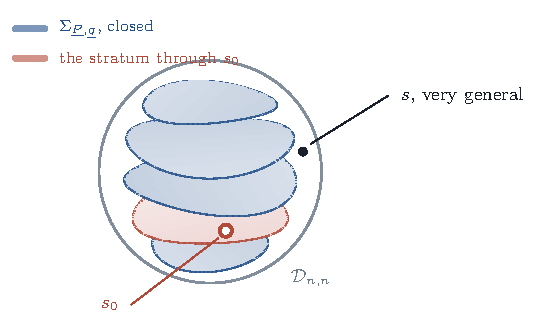
\includegraphics[width=0.88\textwidth]{fig_properness}
\caption{The dichotomy of \Cref{cor:allornothing}. Each stratum
$\Sigma_{\underline{P},\underline{q}}$ is Zariski closed by
\Cref{thm:closedlocus}, and there are countably many of them; the base point
$s_{0}$ of \Cref{thm:everyfamily} lies on one. By \Cref{prop:densealg} the
union of the strata is dense, so a point $s$ off all of them is squeezed
between strata however small a neighbourhood is taken. The conjecture for the
family is the assertion that no such $s$ exists, and by
\Cref{cor:allornothing} it is enough that one stratum has nonempty interior.}
\label{fig:properness}
\end{figure}

The next fact says that case (b) of \Cref{cor:allornothing}, if it occurs,
occurs in an uncomfortable way: the algebraic locus is always dense, so the
two sets in the dichotomy would both be dense and the distinction between them
would be entirely one of measure rather than of position.

\begin{lemma}[Algebraicity is a rational invariant]\label{lem:Ginvariance}
$\Sigma$ is stable under the action of $G(\QQ)$ on $\cD_{n,n}$.
\end{lemma}

\begin{proof}
A point of $\cD_{n,n}$ is a complex structure $J$ on $V_{\RR}$ compatible with
$H$, and $g\in G(\QQ)$ carries $J$ to $gJg^{-1}$. The map $g$ is then
$\QQ$-rational and $\CC$-linear from $(V_{\RR},J)$ to $(V_{\RR},gJg^{-1})$, so
after clearing denominators it induces an isogeny $A_{J}\to A_{gJ}$, whose
graph is an algebraic correspondence. Algebraicity of a rational cohomology
class is preserved by such a correspondence and by its transpose. Finally $g$
lies in $\SU(V,H)$, so by the computation in \Cref{lem:omegadescends} it fixes
the Weil line pointwise, and the class transported from $\omega_{J}$ is
$\omega_{gJ}$.
\end{proof}

\begin{proposition}[The algebraic locus is dense]\label{prop:densealg}
Let $n\ge2$. Then $\Sigma$ is dense in $\cD_{n,n}$ in the analytic topology,
and its image in $\cS$ is dense.\footnote{We should be clear about which
of the two standard density statements this is, because they behave in
opposite ways. For a class that is not flat, the locus where it stays Hodge is
a countable union of proper closed subvarieties, and the content of
\Cref{thm:cdk} is that each of them is algebraic; density there would be a
statement about how special points distribute. For the class $\omega$ of
\Cref{setup:family} the Hodge locus is the whole family by
\Cref{prop:weilline}(ii), so \Cref{thm:cdk} says nothing at all, and the set
that carries information is the algebraic locus instead. The proposition below
is a statement about that set, and its proof uses no Hodge theory: the
algebraic locus is a union of orbits of a group whose rational points are
dense in its real points, and the density is inherited from the group.}
\end{proposition}

\begin{proof}
The hermitian form $H$ has rank $2n\ge4$ over $K$ and signature $(n,n)$, so it
is isotropic over $\RR$; over every $\QQ_{p}$ a hermitian form of rank at
least three over a quadratic extension is isotropic; and hermitian forms over
an imaginary quadratic field satisfy the Hasse principle
\cite[Ch.~10, \S 6]{Sch85}. So $H$ is isotropic over $\QQ$ and $G$ is
$\QQ$-isotropic. The group $G=\SU(V,H)$ is simply connected and almost
$\QQ$-simple, so by Platonov's theorem $G(\QQ)$ is generated by the rational
points of the unipotent radicals of its proper parabolic $\QQ$-subgroups
\cite[Thm.~7.6 and \S 7.2]{PR94}. For a unipotent group $U$ over $\QQ$ the
exponential identifies $U(\QQ)$ with a $\QQ$-vector space inside the
corresponding $\RR$-vector space $U(\RR)$, so $U(\QQ)$ is dense in $U(\RR)$.
The closure of $G(\QQ)$ in $G(\RR)$ therefore contains $U(\RR)$ for every such
$U$, and those generate the identity component $G(\RR)^{+}$, which acts
transitively on $\cD_{n,n}$. Hence every $G(\QQ)$-orbit in $\cD_{n,n}$ is
dense.

By \Cref{thm:everyfamily} the set $\Sigma$ is nonempty, and by
\Cref{lem:Ginvariance} it is $G(\QQ)$-stable, so it contains a dense orbit.
The projection $p$ is open and surjective, so the image is dense.
\end{proof}

\begin{corollary}[The conjecture for Weil type is a non-meagreness
statement]\label{cor:meagre}
Let $n\ge2$. The Hodge conjecture holds for every abelian $2n$-fold of
$(K,-1,n)$-Weil type in the family of \Cref{setup:family} if and only if
$\Sigma$ is non-meagre in $\cD_{n,n}$, and if and only if $\Sigma$ has
nonempty interior.
\end{corollary}

\begin{proof}
If $\Sigma=\cD_{n,n}$ both conditions hold. If not, \Cref{cor:allornothing}(b)
says $\Sigma$ is a countable union of closed sets with empty interior, hence
meagre, and \Cref{thm:residual}(b) says the conjecture fails.
\end{proof}

\subsubsection*{The first criterion: a bound along one orbit}

The proof of \Cref{prop:densealg} produces the dense algebraic locus by moving
one cycle around by rational isogenies, and an isogeny multiplies degrees. So
the dense set it produces is stratified by unbounded data, which is exactly
what stops \Cref{cor:allornothing} from applying. Reversing this gives a
criterion, and it is the sharpest consequence of \Cref{thm:closedlocus} we
know how to state.

\begin{theorem}[A bound along the orbit closes the family]\label{thm:degreebound}
Let $n\ge2$ and let $s_{0}\in\Sigma$ be one of the base points supplied by
\Cref{thm:everyfamily}. Suppose that there is a finite set $\mathcal{T}$ of pairs
$(\underline{P},\underline{q})$ such that for every $g\in G(\QQ)$ the class
$\omega_{g\cdot s_{0}}$ is represented by some cycle whose Hilbert data lies
in $\mathcal{T}$. Then $\Sigma=\cD_{n,n}$, and the Hodge conjecture holds in every
degree for every abelian $2n$-fold of $(K,-1,n)$-Weil type with
$\Hg(A)=\SU(V,H)$ in that family.
\end{theorem}

\begin{remark}[The cycle is chosen, not transported]\label{rem:chosencycle}
The hypothesis quantifies over representing cycles at each point of the orbit
and asks only that one of them, at each point, be of bounded complexity. An
earlier form of this statement fixed the cycle, taking at $g\cdot s_{0}$ the
transport of the cycle at $s_{0}$ along the isogeny of
\Cref{lem:Ginvariance}. That form is stronger, and \Cref{thm:p1forces} below
shows that it is too strong to be usable: for a base cycle with a component of
finite stabiliser the transported data is unbounded, so its hypothesis is never
satisfied. The proof below uses only the weaker hypothesis, which is what the
covering argument needs.
\end{remark}

\begin{proof}
The orbit $G(\QQ)\cdot s_{0}$ is dense by the proof of \Cref{prop:densealg},
and by hypothesis it is the union of the finitely many sets
$G(\QQ)\cdot s_{0}\cap p^{-1}(\Sigma_{\underline{P},\underline{q}})$ with
$(\underline{P},\underline{q})\in\mathcal{T}$. A finite
union of closed sets is dense only if one of them is, so one
$p^{-1}(\Sigma_{\underline{P},\underline{q}})$ is dense; it is closed in the
analytic topology, hence equals $\cD_{n,n}$. Now apply
\Cref{thm:residual}(a).
\end{proof}

The hypothesis of \Cref{thm:degreebound} can be sharpened, and the sharpening
says which half of the Hilbert data is at issue. The leading coefficient is
not.

\begin{proposition}[The leading coefficient is constant on the orbit]
\label{prop:leadingconstant}
Let $s_{0}\in\Sigma$ and $g\in G(\QQ)$, and let $\omega_{s}$ denote the Weil
class at $s$ and $\eta$ the polarisation class. Then
\[
  \int_{A_{g\cdot s_{0}}}\omega_{g\cdot s_{0}}\cdot\frac{\eta^{n}}{n!}
  \;=\;\int_{A_{s_{0}}}\omega_{s_{0}}\cdot\frac{\eta^{n}}{n!},
\]
so the degree of the transported class with respect to the polarisation, which
is the leading coefficient of the Hilbert polynomial of any cycle
representing it, is the same at every point of the orbit.
\end{proposition}

\begin{proof}
By \Cref{lem:Ginvariance} the correspondence transporting the class is induced
by a $\QQ$-rational map which lies in $\SU(V,H)$, so it preserves the
hermitian form and hence the polarisation class, and by
\Cref{lem:omegadescends} it fixes the Weil line pointwise. An intersection
number of classes preserved by a correspondence is preserved by it. The
identification of the number with the leading coefficient is
Hirzebruch--Riemann--Roch on $A$, the higher coefficients involving the
structure sheaf of the cycle and not only its class.
\end{proof}

\begin{remark}[Where the unboundedness can only come from]
\label{rem:whereunbounded}
Write the transported cycle as a difference $\xi^{+}-\xi^{-}$ of effective
cycles. By \Cref{prop:leadingconstant} the difference of their degrees is
constant along the orbit, and by the boundedness of the Chow variety of
effective cycles of bounded degree in a fixed polarised variety, if
$\deg\xi^{+}$ were bounded along the orbit then only finitely many tuples
$(\underline{P},\underline{q})$ could occur and \Cref{thm:degreebound} would
apply. So the hypothesis of that theorem is equivalent to a bound on the
effective part alone.

That is not a formality, and the mechanism that threatens it is visible. The
transport at $g$ is by the isogeny obtained from $g$ by clearing denominators;
if $g$ has denominator $m$ on the reference lattice, which has rank $4n$, the
isogeny has degree a divisor of $m^{4n}$, and pushing a cycle forward along it
multiplies the multiplicities by factors of that order. The rational points of
$G$ are dense precisely because their denominators are unbounded, so along any
orbit dense enough to be useful the isogeny degrees are unbounded as well.
What \Cref{thm:degreebound} asks is that the cycles nevertheless simplify: that
after each transport the class $\omega$, whose degree has not changed, admits
an effective representation no more complicated than before. Nothing in this
paper decides that, and we do not know how to decide it. The content of the
present remark is only that the question has been reduced from the whole
Hilbert datum to the degree of the effective part, and that the part of the
datum which is determined by cohomology is already constant.
\end{remark}

\subsubsection*{What the transport does, exactly}

The mechanism of \Cref{rem:whereunbounded} can be computed rather than
described, and computing it decides one of the two readings of (P1). Write
$\Lambda$ for the reference lattice, of rank $4n$ over $\ZZ$, and $E$ for the
alternating form of the polarisation, so that a point $s$ of $\cD_{n,n}$ is a
complex structure on $\Lambda\otimes\RR$ and $A_{s}=(\Lambda\otimes\RR)/\Lambda$.
Throughout, $G=\dim A_{s}=2n$ and a component of a cycle representing
$\omega_{s}$ has dimension $n$.

\begin{lemma}[The transport, in coordinates]\label{lem:transport}
Let $g\in G(\QQ)$ and let $c=c(g)$ be the least positive integer with
$cg\Lambda\subseteq\Lambda$. Then $\varphi_{g}:=cg$ induces an isogeny
$A_{s_{0}}\to A_{g\cdot s_{0}}$ with
\begin{enumerate}[label=\textup{(\roman*)},nosep,leftmargin=2.6em]
\item $\deg\varphi_{g}=c^{4n}$;
\item $\varphi_{g}^{*}\eta_{g\cdot s_{0}}=c^{2}\eta_{s_{0}}$ and
  $\varphi_{g}^{*}\omega_{g\cdot s_{0}}=c^{2n}\omega_{s_{0}}$;
\item the transported cycle representing $\omega_{g\cdot s_{0}}$ is
  $c^{2n-4n}\,\varphi_{g*}(Z)$, where $Z$ represents $\omega_{s_{0}}$.
\end{enumerate}
Moreover $\sup_{g\in G(\QQ)}c(g)=\infty$.
\end{lemma}

\begin{proof}
(i) The index of $cg\Lambda$ in $\Lambda$ is $|\det_{\QQ}(cg)|
=c^{4n}|\det_{\QQ}g|$, and $\det_{\QQ}g=\Nm_{K/\QQ}(\det_{K}g)=1$ for
$g\in\SU(V,H)$.

(ii) $g$ preserves $E$, so $(cg)^{*}E=c^{2}E$, which is the first identity.
On $H^{2n}=\bigwedge^{2n}(\Lambda^{\vee}\otimes\QQ)$ the map
$\varphi_{g}^{*}$ is $c^{2n}\bigwedge^{2n}g^{\vee}$, and $g\in\SU(V,H)$ fixes
the Weil line pointwise by \Cref{lem:omegadescends}.

(iii) $\varphi_{g*}\varphi_{g}^{*}=\deg\varphi_{g}$, so
$\omega_{g\cdot s_{0}}=(\deg\varphi_{g})^{-1}\varphi_{g*}
\varphi_{g}^{*}\omega_{g\cdot s_{0}}
=c^{2n-4n}\varphi_{g*}\omega_{s_{0}}$ by (i) and (ii).

For the last sentence, $G$ is $\QQ$-isotropic by the proof of
\Cref{prop:densealg}, so it has a proper parabolic $\QQ$-subgroup whose
unipotent radical $U$ satisfies $U(\QQ)\cong\QQ^{k}$ with $k\ge1$ through the
exponential; the entries of $u\in U(\QQ)$ are $\QQ$-linear in that coordinate,
so $c(u)$ is unbounded on $U(\QQ)$. Item (XXXVII) of \Cref{sec:verification}
verifies (i) and (ii) on an explicit sample of such $u$ with $c$ up to $29$,
for $2n=4,6,8$.
\end{proof}

\begin{lemma}[The multiplicity is the stabiliser met by the kernel]
\label{lem:multiplicity}
Let $\varphi\colon A\to A'$ be an isogeny of abelian varieties and $Z\subseteq A$
an integral closed subvariety. Put
$G(Z)=\{x\in A:Z+x=Z\}$, a closed algebraic subgroup. Then
\[
  \varphi_{*}[Z]=m\,[\varphi(Z)],\qquad
  m=\bigl|\ker\varphi\cap G(Z)\bigr| .
\]
If moreover $\dim Z=n$ and $\varphi^{*}\eta'=c^{2}\eta$, then
\[
  \deg_{\eta'}\varphi(Z)=\frac{c^{2n}}{m}\,\deg_{\eta}Z .
\]
\end{lemma}

\begin{proof}
The map $\varphi|_{Z}\colon Z\to\varphi(Z)$ is finite and surjective, and its
degree $m$ is the number of points of a general fibre. For $z\in Z$ the fibre
through $z$ is $Z\cap(z+\ker\varphi)$, which as a set of translations is
$\{t\in\ker\varphi:z+t\in Z\}$. For a fixed $t$ the locus
$\{z\in Z:z+t\in Z\}=Z\cap(Z-t)$ is all of $Z$ when $t\in G(Z)$ and a proper
closed subset otherwise; since $\ker\varphi$ is finite, a general $z$ avoids
the finitely many proper subsets, and there
$\{t\in\ker\varphi:z+t\in Z\}=\ker\varphi\cap G(Z)$. This is the first
identity, and $\varphi_{*}[Z]=m[\varphi(Z)]$ by the definition of the
pushforward of cycles.

For the degree, the projection formula gives
\[
  m\deg_{\eta'}\varphi(Z)=\int\varphi_{*}[Z]\cdot\frac{\eta'^{n}}{n!}
  =\int[Z]\cdot\frac{(\varphi^{*}\eta')^{n}}{n!}
  =c^{2n}\int[Z]\cdot\frac{\eta^{n}}{n!}=c^{2n}\deg_{\eta}Z .
\]
Item (XXXVII) verifies both identities for subtori of an abelian fourfold,
with $m$ computed as a lattice index by Smith normal form and the degrees as
Pfaffians; there the two cases are visible side by side, a subtorus preserved
by $\varphi$ having $m=c^{2n}$ and image degree constant, and one not
preserved having $m=c^{2n-1}$ and image degree growing linearly in $c$.
\end{proof}

\begin{theorem}[What \textup{(P1)} forces on the base cycle]\label{thm:p1forces}
Let $s_{0}\in\Sigma$ and let $Z=\sum_{i}q_{i}Z_{i}$, with $q_{i}\ne0$ and the
$Z_{i}$ integral of dimension $n$, represent $\omega_{s_{0}}$.
\begin{enumerate}[label=\textup{(\roman*)},leftmargin=2.6em,itemsep=2pt]
\item For $g\in G(\QQ)$ the transported cycle is
  $\sum_{i}c(g)^{2n-4n}m_{i}(g)\,q_{i}\,[\varphi_{g}(Z_{i})]$ with
  $m_{i}(g)=|\ker\varphi_{g}\cap G(Z_{i})|$, and the $i$-th component has
  degree $c(g)^{2n}\deg_{\eta}(Z_{i})/m_{i}(g)$.
\item If some $Z_{i}$ has finite stabiliser $G(Z_{i})$, then
  $\deg\varphi_{g}(Z_{i})\ge c(g)^{2n}\deg_{\eta}(Z_{i})/|G(Z_{i})|$, which is
  unbounded on $G(\QQ)$. The Hilbert data of the transported cycle then takes
  infinitely many values, and the hypothesis of \Cref{thm:degreebound} in the
  form that fixes the transported cycle is not satisfied by $Z$.
\item Consequently, a base cycle for which the transported data is bounded
  must have every component of positive-dimensional stabiliser, that is, every
  $Z_{i}$ must be stable under translation by a positive-dimensional abelian
  subvariety of $A_{s_{0}}$.
\end{enumerate}
\end{theorem}

\begin{proof}
(i) is \Cref{lem:transport}(iii) and \Cref{lem:multiplicity}.

(ii) $\ker\varphi_{g}\cap G(Z_{i})\subseteq G(Z_{i})$, so
$m_{i}(g)\le|G(Z_{i})|$, a constant; the displayed bound is (i), and $c(g)$ is
unbounded by \Cref{lem:transport}. Distinct degrees of the components give
distinct Hilbert polynomials, so the data takes infinitely many values.

(iii) is the contrapositive of (ii), together with the fact that an algebraic
subgroup of positive dimension in an abelian variety has an abelian subvariety
of positive dimension as its identity component.
\end{proof}

\begin{remark}[What this settles and what it leaves]\label{rem:p1meaning}
Three things follow, and we separate them.

The statement (P1) has two readings, and one of them is now closed. Read with
the cycle fixed at $s_{0}$ and transported, it fails for every base cycle this
paper writes down: those cycles are intersections of divisors, and an
intersection of $n$ divisors on an abelian $2n$-fold has finite stabiliser
unless the divisors are pulled back from a quotient, which the ones here are
not. Read with the cycle chosen afresh at each point of the orbit, which is
the form \Cref{thm:degreebound} now takes, it is untouched by
\Cref{thm:p1forces} and remains open.

The two readings are different, and the difference is the content of
\Cref{lem:multiplicity}. The class $\omega_{g\cdot s_{0}}$ has constant degree
along the orbit, by \Cref{prop:leadingconstant}; what grows is the complexity
of the particular representative the transport produces, and it grows because
the isogeny spreads each component out by the factor $c^{2n}/m_{i}$. A
representative of bounded complexity may well exist at every point; the
transport does not find it.

The third is a demand on any future attempt at (P1). It must either produce a
base cycle supported on subvarieties with positive-dimensional stabiliser,
which for a Weil class is a strong and possibly impossible requirement, or
abandon the transport and bound instead the minimal complexity of a
representative, which is a statement about the Chow variety of the family and
not about any one cycle. We do not know how to do either.
\end{remark}

The bound on the minimal complexity is the form in
which \Cref{thm:degreebound} now stands. It is the weakest hypothesis under
which the covering argument runs, and it is therefore the form in which (P1)
would have to be attacked. The next theorem decides it, and the answer is that
there is nothing there to attack: the hypothesis is not a sufficient condition
for the conjecture on the family but another way of writing it.

\begin{theorem}[The bounded form is the conjecture itself]\label{thm:p1equivalent}
Let $n\ge2$, let $s_{0}\in\Sigma$ and keep \Cref{setup:family}. The following
are equivalent.
\begin{enumerate}[label=\textup{(\alph*)},leftmargin=2.6em,itemsep=2pt]
\item There is a finite set $\mathcal{T}$ of pairs
  $(\underline{P},\underline{q})$ such that at every point of the orbit
  $G(\QQ)\cdot s_{0}$ the class $\omega$ is represented by a cycle whose
  Hilbert data lies in $\mathcal{T}$; that is, \textup{(P1)} holds at
  $s_{0}$.
\item There is a single pair $(\underline{P},\underline{q})$ such that at
  every point of $\cD_{n,n}$, not merely of the orbit, the class $\omega$ is
  represented by a cycle with that datum.
\item $\Sigma=\cD_{n,n}$.
\item $\mathbf{W}(K,n,\delta)$ holds, that is, the Weil classes are algebraic
  on every member of the family.
\end{enumerate}
In particular \Cref{thm:degreebound} is an equivalence, and \textup{(P1)} is a
reformulation of the conjecture for the family and not a reduction of it. The
same holds for every CM field, with \Cref{thm:cmpropagation}(iv) in place of
\Cref{thm:degreebound}.
\end{theorem}

\begin{proof}
(a) implies (c) is \Cref{thm:degreebound}. (b) implies (a) is immediate, the
orbit being contained in $\cD_{n,n}$ and $\mathcal{T}$ being the one pair.
(c) is equivalent to (d) by \Cref{thm:residual}(a) and (b).

It remains to deduce (b) from (c). If $\Sigma=\cD_{n,n}$ then $\Sigma$ has
nonempty interior, and the first paragraph of the proof of
\Cref{cor:allornothing} shows that some
$\Sigma_{\underline{P},\underline{q}}$ is then all of $\cS$: the countably
many sets $\Sigma_{\underline{P},\underline{q}}\cap U$ are closed in a
nonempty connected open $U\subseteq\cS$ and cover it, a connected complex
manifold is a Baire space, so one of them has nonempty interior in $U$, and a
proper Zariski closed subvariety of the irreducible variety $\cS$ has empty
interior. By the definition of $\Sigma_{\underline{P},\underline{q}}$ in
\Cref{thm:closedlocus} as the image of a proper morphism, every $s\in\cS$
then carries a tuple $\underline{Z}$ of subschemes with Hilbert polynomials
$\underline{P}$ and $\sum_{i}q_{i}[Z_{i}]=\omega$, which is (b).

For a CM field the same argument applies verbatim, using
\Cref{thm:cmpropagation}(iii) in place of \Cref{thm:closedlocus} and
\Cref{cor:allornothing}.
\end{proof}

\begin{remark}[What is left of the first criterion]\label{rem:p1collapse}
\Cref{thm:p1equivalent} removes (P1) from the list of things that would close
the family, and we should be exact about what it does and does not say.

It does not say that \Cref{thm:degreebound} is false or that its proof is
defective. The implication it proves is correct, and the covering argument is
the only place in this paper where density of the rational orbit is converted
into a global statement. What the theorem says is that the implication has a
converse, so that the hypothesis is no weaker than the conclusion. A criterion
of that kind cannot be used: verifying it at one family is exactly as hard as
proving the conjecture for that family, no more and no less.

Nor does it say that the boundedness is uninteresting. It is a concrete
finiteness statement about the Chow variety of the universal family, and it is
the only reformulation of $\mathbf{W}(K,n,\delta)$ we know that mentions
neither Hodge theory nor deformation theory. What it is not is a step.

The two forms of the propagation statement are therefore not on the same
footing, and we had them on the same footing until now. (P2) remains a genuine
sufficient condition: injectivity of one semiregularity map at one point
implies the conjecture for the whole family, and nothing here shows the
converse, nor do we see how it could, since $\Sigma=\cD_{n,n}$ says nothing
about the deformation theory of any particular perfect complex. So the
propagation half of the frontier is the single statement (P2), and the
constraints \Cref{thm:p2forces} and \Cref{cor:p2shape} place on it are the
constraints on the whole of that half.
\end{remark}

At the quaternionic points of \Cref{setup:quat} the mechanism of
\Cref{rem:whereunbounded} can be seen explicitly. Take $n=2$ and the integral
lattice
$\Lambda_{b}=\cO_{b}^{2}$, $\cO_{b}=\ZZ\langle 1,i,j,ij\rangle$, for
$b\in\ZZ_{>0}$. Put
\[
  g_{b}(x,y)=E_{b}(jx,y),\qquad
  \lambda_{b}(x,y)=-\tfrac{1}{d}\,g_{b}(ix,y),\qquad
  Z_{b}=g_{b}^{2}-d\lambda_{b}^{2},\qquad Z'_{b}=2g_{b}\lambda_{b},
\]
so that $Z_{b}+\sqrt{-d}\,Z'_{b}=(g_{b}+\sqrt{-d}\,\lambda_{b})^{2}$ and
$Z_{b},Z'_{b}$ span the Weil plane. Write $x\in\cO_{b}$ as $x=u+vj$ with
$u,v\in\ZZ[i]$; the pair $(\Lambda_{b},i)$ is then the same $\ZZ[i]$-module
$\ZZ[i]^{4}$ for every $b$, and we use this identification throughout.

\begin{proposition}[The quaternionic Weil cycle is a square multiple]
\label{prop:quatdivisible}
With these data, for every $b\in\ZZ_{>0}$:
\begin{enumerate}[label=\textup{(\roman*)},nosep]
\item $E_{b}=E_{u}+b\,E_{v}$, $g_{b}=b\,g_{1}$ and $\lambda_{b}=b\,\lambda_{1}$,
  where $E_{u},E_{v},g_{1},\lambda_{1}$ are integral on $\ZZ[i]^{4}$ and do not
  depend on $b$; in particular $g_{1},\lambda_{1}\in\mathrm{NS}(A_{b})$;
\item $Z_{b}=b^{2}Z_{1}$ and $Z'_{b}=b^{2}Z'_{1}$ in $\mathrm{CH}^{2}(A_{b})$
  modulo algebraically trivial cycles, for every choice of line bundles
  representing $g_{b},\lambda_{b}$; in cohomology the equalities hold in
  $\wedge^{4}\Lambda^{*}$;
\item $\int\eta_{b}^{4}=b^{2}\int\eta_{1}^{4}$,
  $\int g_{b}^{2}\eta_{b}^{2}=-\tfrac{b}{3}\int\eta_{b}^{4}$ and
  $\int Z_{b}^{2}=\tfrac{4b^{2}}{3}\int\eta_{b}^{4}$, so that
  $(\int g_{b}^{2}\eta_{b}^{2})^{2}=\tfrac{1}{12}\int Z_{b}^{2}\int\eta_{b}^{4}$;
\item for $\alpha\in K^{\times}$ the element $\alpha j$ generates the same
  algebra at the same point, and replacing $j$ by $\alpha j$ multiplies the
  two ratios in \textup{(iii)} by $N(\alpha)$ and $N(\alpha)^{2}$.
\end{enumerate}
\end{proposition}

\begin{proof}
For $x=u+vj$ one has $\bbar{x}=\bbar{u}-vj$, and the relations $ju=\bbar{u}j$,
$j^{2}=b$ give
$\bbar{x}\,i\,y\equiv\bbar{u}\,i\,u'+b\,v\,i\,\bbar{v'}$ modulo $Kj$. Since
$\mathrm{trd}$ vanishes on $Kj$ and restricts to $\mathrm{tr}_{K/\QQ}$ on $K$,
\[
  E_{b}(x,y)=\textstyle\sum_{k}a_{k}\bigl(\mathrm{tr}(i\,\bbar{u_{k}}u'_{k})
  +b\,\mathrm{tr}(i\,v_{k}\bbar{v'_{k}})\bigr).
\]
From $jx=b\bbar{v}+\bbar{u}j$ one reads off
$g_{b}(x,y)=b\sum_{k}a_{k}\bigl(\mathrm{tr}(i\,v_{k}u'_{k})
+\mathrm{tr}(i\,\bbar{u_{k}}\bbar{v'_{k}})\bigr)$, which is $b\,g_{1}$, and
$\lambda_{b}=b\lambda_{1}$ follows. The traces take integral values on
$\ZZ[i]$, and $g_{1}=b^{-1}g_{b}$ is a rational multiple of a Hodge class,
which proves (i). Then $g_{b}+\sqrt{-d}\,\lambda_{b}=b(g_{1}+\sqrt{-d}\,\lambda_{1})$
and (ii) holds in cohomology. Choosing $L,M$ with $c_{1}(L)=g_{1}$,
$c_{1}(M)=\lambda_{1}$, the cycle $c_{1}(L^{b})^{2}-d\,c_{1}(M^{b})^{2}$ equals
$b^{2}(c_{1}(L)^{2}-d\,c_{1}(M)^{2})$ in $\mathrm{CH}^{2}(A_{b})$; another
choice changes both sides by algebraically trivial cycles.

For (iii), $E_{u}$ and $E_{v}$ live on complementary halves $U,V'$ of
$\Lambda\otimes\QQ$ of rank four, so $\eta_{u}^{3}=\eta_{v}^{3}=0$ and
$\int\eta_{b}^{4}=6b^{2}\int\eta_{u}^{2}\eta_{v}^{2}$. The form $g_{1}$ pairs
$U$ with $V'$, so $g_{1}^{2}\in\wedge^{2}U^{*}\otimes\wedge^{2}V'^{*}$, and
only the mixed term survives in
$\int g_{b}^{2}\eta_{b}^{2}=2b^{3}\int g_{1}^{2}\eta_{u}\eta_{v}$; likewise
$\int Z_{b}^{2}=b^{4}\int Z_{1}^{2}$. Hence the ratios
$\int g_{b}^{2}\eta_{b}^{2}/\int\eta_{b}^{4}$ and
$\int Z_{b}^{2}/\int\eta_{b}^{4}$ are $b$ and $b^{2}$ times their values at
$b=1$, which are $-1/3$ and $4/3$ by direct evaluation. For (iv), $(\alpha j)^{2}=N(\alpha)b$ and
$g_{\alpha j}+\sqrt{-d}\,\lambda_{\alpha j}$ is $\alpha$ or $\bbar{\alpha}$
times $g_{j}+\sqrt{-d}\,\lambda_{j}$.
\end{proof}

Item (XXIII) of \Cref{sec:verification} confirms (i) to (iv) in exact
arithmetic for $d\in\{1,3\}$, two weight vectors and fifteen values of $b$ up
to $101$. It also computes the integral Weil lattice
$\HW_{\ZZ}=(\QQ Z_{b}+\QQ Z'_{b})\cap\wedge^{4}\Lambda^{*}$ and the
sublattice spanned inside it by products of two integral divisor classes: for
$d\in\{1,2,3,7\}$, three weight vectors and seven values of $b$, the Gram
matrix of $\HW_{\ZZ}$ is $\mathrm{diag}(8d,8d^{2})$ and the index is
$2(a_{1}a_{2})^{2}$, both independent of $b$.

\begin{remark}[The multiple sits in the polarisation]\label{rem:quatdivisible}
At these points the Weil class carries no multiple that grows with $b$ once
it is written in integral terms: by \Cref{prop:quatdivisible}(ii) it is
$b^{2}Z_{1}$, with $Z_{1}$ one integral algebraic cycle built from the two
fixed divisor classes $g_{1},\lambda_{1}$. The factor that the orbit argument
would otherwise have to absorb into the coefficients $\underline{q}$ of
\Cref{thm:degreebound} is therefore absent. What grows is the polarisation:
$\int\eta_{b}^{4}=b^{2}\int\eta_{1}^{4}$, so the points $A_{b}$ carry
polarisations of unbounded degree, and an isogeny carrying $\eta_{b}$ to the
polarisation of one fixed family has degree $\int\eta_{b}^{4}/\int\eta^{4}$,
which grows like $b^{2}$. This is the unbounded isogeny degree of
\Cref{rem:whereunbounded}, located at an explicit family of points, and it is
untouched by the integrality of $Z_{1}$.
\end{remark}

The base points of \Cref{thm:everyfamily}, and every algebraicity statement
for Weil classes proved in this paper, represent $\omega$ through products of
divisor classes. The next result says that a representation of that kind can
hold with bounded degrees only on a nowhere dense set, so the bound asked for
in \Cref{thm:degreebound} has to come from cycles that are not products of
divisors. For a class $x\in H^{2}(A_{s},\RR)$ put
\[
  t(x)=\frac{\int x\,\eta^{2n-1}}{\int\eta^{2n}},\qquad
  I(x)=t(x)^{2}\!\int\eta^{2n}-\int\bigl(x-t(x)\eta\bigr)^{2}\eta^{2n-2}.
\]
Since $\cD_{n,n}$ is contractible, the local system $R^{2}\pi_{*}\ZZ$ is
trivial; write $H^{2}_{\ZZ}$ for its fibre, identified with $H^{2}(A_{s},\ZZ)$
at every $s$. Both $t$ and $I$ are polynomial functions on $H^{2}_{\ZZ}$ and
do not depend on $s$.

\begin{lemma}[The Hodge norm of a divisor]\label{lem:nefnorm}
Let $h_{s}$ be the Hodge norm on $H^{2}(A_{s},\RR)$ defined by the
polarisation, normalised by $h_{s}(\eta)=\int\eta^{2n}$. Then
\begin{enumerate}[label=\textup{(\roman*)},nosep]
\item $h_{s}(x)=I(x)$ for every real class $x$ of type $(1,1)$ at $s$;
\item if $D$ is an effective divisor on $A_{s}$ then
  $I([D])\le 2\bigl(\int[D]\eta^{2n-1}\bigr)^{2}\big/\!\int\eta^{2n}$.
\end{enumerate}
\end{lemma}

\begin{proof}
Write $x=t\eta+x_{0}$ with $t=t(x)$, so that $x_{0}$ is primitive. The
Lefschetz decomposition is orthogonal for $h_{s}$, and on primitive classes
$h_{s}(x_{0})=-\int x_{0}\wedge C_{s}x_{0}\wedge\eta^{2n-2}$, where $C_{s}$ is
the Weil operator, positive by the Hodge--Riemann relations. For $x_{0}$ of type
$(1,1)$, $C_{s}x_{0}=x_{0}$, which gives (i). An effective divisor on an
abelian variety is nef, since a translate of it meets any given curve
properly, so $\int[D]^{2}\eta^{2n-2}\ge0$. Expanding,
$\int[D]^{2}\eta^{2n-2}=t^{2}\int\eta^{2n}+\int x_{0}^{2}\eta^{2n-2}$, hence
$-\int x_{0}^{2}\eta^{2n-2}\le t^{2}\int\eta^{2n}$ and
$I([D])\le2t^{2}\int\eta^{2n}$, which is (ii).
\end{proof}

\begin{proposition}[Divisor products of bounded degree]\label{prop:divroute}
In \Cref{setup:family}, fix $C>0$ and let $\Sigma_{C}\subset\cD_{n,n}$ be the
set of points $s$ at which $\omega_{s}$ is a $\QQ$-linear combination of
classes $[D_{1}]\cdots[D_{n}]$ with every $D_{i}$ an effective divisor on
$A_{s}$ of degree $\int[D_{i}]\eta^{2n-1}\le C$. Then $\Sigma_{C}$ is
contained in a locally finite union of proper closed analytic subsets of
$\cD_{n,n}$. In particular $\Sigma_{C}$ is nowhere dense, and on any dense
subset of $\cD_{n,n}$ at which $\omega$ is a combination of products of
effective divisors the degrees of those divisors are unbounded on every
nonempty open set.
\end{proposition}

\begin{proof}
For $x\in H^{2}_{\ZZ}$ let $\mathrm{Hdg}(x)\subset\cD_{n,n}$ be the
closed analytic set where $x$ is of type $(1,1)$. If $x\notin\QQ\eta$ it is
proper, because $\NS(A_{s})\otimes\QQ=\QQ\eta$ at a very general point by
\Cref{lem:genericNS}. Let $s\in\Sigma_{C}$. Not every $[D_{i}]$ in the
representation lies in $\QQ\eta$, since $\QQ\eta^{n}$ and the Weil line carry
different characters by \Cref{lem:charsdiffer}. So $s\in\mathrm{Hdg}(x)$ for
some $x$ in
\[
  X_{C}=\bigl\{x\in H^{2}_{\ZZ}\setminus\QQ\eta\;:\;
  I(x)\le 2C^{2}/\textstyle\int\eta^{2n}\bigr\},
\]
by \Cref{lem:nefnorm}(ii). Now let $U\subset\cD_{n,n}$ be open with compact
closure and $s_{0}\in U$. The Hodge norm depends continuously on the point, so
$h_{s_{0}}\le c_{U}\,h_{s}$ for some $c_{U}$ and all $s\in U$. If
$\mathrm{Hdg}(x)$ meets $U$ at $s$ and $x\in X_{C}$, then by
\Cref{lem:nefnorm}(i)
$h_{s_{0}}(x)\le c_{U}h_{s}(x)=c_{U}I(x)\le 2c_{U}C^{2}/\int\eta^{2n}$, and
only finitely many integral classes satisfy this. So the sets
$\mathrm{Hdg}(x)$, $x\in X_{C}$, form a locally finite family of proper closed
analytic subsets. Their union is closed with empty interior in the connected
manifold $\cD_{n,n}$, and it contains $\Sigma_{C}$.
\end{proof}

\begin{remark}[What the proposition closes]\label{rem:divroute}
The loci on which this paper proves $\omega$ algebraic are the split,
quaternionic and product loci and their translates under $G(\QQ)$, and on
each of them $\omega$ is a rational polynomial in divisor classes, since an
isogeny carries $\NS\otimes\QQ$ isomorphically. \Cref{prop:divroute} shows that no
bounded family of such cycles covers a dense set, so the finiteness in
\Cref{thm:degreebound} cannot be obtained by bounding the divisors that
produce $\omega$ at the points where it is known to be algebraic. It has to
come from the transported cycles of \Cref{lem:Ginvariance} themselves, which
are push-forwards along isogenies and not products of divisors on the target.
That is the unbounded isogeny degree of \Cref{rem:whereunbounded} and
\Cref{rem:quatdivisible}, now shown to be unavoidable for the divisorial
constructions. The argument uses nothing about $\omega$ beyond the fact that it
is not a multiple of $\eta^{n}$, and nothing about the family beyond the
generic Picard number, so it applies equally to any variational argument that
feeds on divisor products.
\end{remark}

At $n=2$ the phenomenon can be exhibited on one fixed polarised lattice. Take
$\Lambda=\cO^{2}$ with $\cO=\ZZ\langle1,i,j,ij\rangle$, $i^{2}=-d$, $j^{2}=1$,
and $E$ as in \eqref{eq:quatE}; this is one member of the family, with its
lattice and polarisation fixed. Let
$R=\{x:\ x(iu,v)=x(u,iv)\}\subset H^{2}(\Lambda,\QQ)$ be the space of
$K$-bilinear classes, where the divisor classes of the quaternionic points
live, and for $x\in R$ let $\phi_{x}=E^{-1}x$, so that $x(u,v)=E(\phi_{x}u,v)$.

\begin{proposition}[A pencil of quaternionic loci]\label{prop:pencil}
In this setting, for $d\in\{1,3\}$:
\begin{enumerate}[label=\textup{(\roman*)},nosep]
\item $R\cap H^{2}(\Lambda,\ZZ)$ has rank $12$, every $x\in R$ has $t(x)=0$,
  and $I(x)=\tfrac{1}{24}\,\mathrm{tr}(\phi_{x}^{2})\int\eta^{4}$; the form $I$
  has signature $(8,4)$ on $R$;
\item there are $x,y\in R\cap H^{2}(\Lambda,\ZZ)$ such that
  $\phi_{x+ky}^{2}=\beta(k)$ is a positive rational scalar for every
  $k\in\ZZ$, with $\beta(k)=\tfrac12+\tfrac12k+\tfrac14k^{2}$ for $d=1$ and
  $\beta(k)=\tfrac19+\tfrac29k^{2}$ for $d=3$;
\item for every $k$ the set $\mathrm{Hdg}(x+ky)$ is a quaternionic locus
  with algebra $(-d,\beta(k))$, nonempty of dimension $3$, and loci with
  different values of $\beta$ are not related by any automorphism of
  $(\Lambda,E,i)$;
\item at a very general point of $\mathrm{Hdg}(x+ky)$ one has
  $\NS\otimes\QQ=\QQ\eta\oplus\QQ x_{k}\oplus\QQ\,x_{k}(i\cdot,\cdot)$ with
  $x_{k}=x+ky$, and for every $k\in\ZZ$ the minimum $\mu_{k}$ of $I$ on
  $\NS\setminus\QQ\eta$ satisfies
  $\mu_{k}\ge\beta(k)\big/\bigl(3N_{d}^{2}\int\eta^{4}\bigr)$, with $N_{1}=2$
  and $N_{3}=4$.
\end{enumerate}
Consequently, at a very general point of $\mathrm{Hdg}(x+ky)$ every effective
divisor whose class is not a multiple of $\eta$ has degree at least
$\sqrt{\beta(k)/6}\,/N_{d}$, which grows linearly in $|k|$.
\end{proposition}

\begin{proof}
(i) and (ii) are finite exact computations, item (XXIV) of
\Cref{sec:verification}: the trace identity is checked on all pairs of a basis
of $R\cap H^{2}(\Lambda,\ZZ)$, which proves it on $R$ by bilinearity, and in
(ii) the three matrices $\phi_{x}^{2}$, $\phi_{y}^{2}$ and
$\phi_{x}\phi_{y}+\phi_{y}\phi_{x}$ are scalar, so
$\phi_{x+ky}^{2}=\phi_{x}^{2}+k(\phi_{x}\phi_{y}+\phi_{y}\phi_{x})+k^{2}\phi_{y}^{2}$
is scalar for every $k$; $\beta$ has positive leading coefficient and negative
discriminant. For (iii) write $\phi=\phi_{x+ky}$ and $\beta=\beta(k)$. The map
$\phi$ is $E$-self-adjoint, anticommutes with $i$, and $\phi^{2}=\beta>0$, so
$V_{\RR}=V_{+}\oplus V_{-}$ with $V_{\pm}$ the $\pm\sqrt{\beta}$ eigenspaces,
$E$-orthogonal to each other, and $i$ exchanges them. A complex structure $J$
on $V_{+}$ compatible with $E|_{V_{+}}$, extended to $V_{-}=iV_{+}$ by
$J(iw)=iJw$, commutes with $i$ and $\phi$ and is compatible with $E$, and $i$
has eigenvalues $\pm\sqrt{-d}$ each with multiplicity $2$ on $V^{1,0}$; so
these $J$ are points of $\cD_{2,2}$ at which $x+ky$ is of type $(1,1)$, and
they form a copy of the Siegel space of $V_{+}$, of dimension $3$, in
agreement with \Cref{prop:lagrangian}. An automorphism $\gamma$
of $(\Lambda,E,i)$ sends $\phi_{x}$ to $\gamma\phi_{x}\gamma^{-1}$ and so
preserves $\mathrm{tr}(\phi_{x}^{2})$.

For the first half of (iv), let $S_{k}\subset\cD_{2,2}$ be the Siegel space
just described and $\mathcal{C}_{k}\subset\Sp(V_{\RR},E)$ the centraliser of
$i$ and $\phi$. An element of $\mathcal{C}_{k}$ preserves $V_{+}$ and is
determined by its restriction there, because it commutes with $i$, so
$\mathcal{C}_{k}\cong\Sp(V_{+})$, acting on $V_{\RR}=V_{+}\oplus iV_{+}$ as
$g\oplus igi^{-1}$. A real class is of type $(1,1)$ at $J$ exactly when it is
invariant under $J$. The points of $S_{k}$ form one orbit
$\{gJ_{0}g^{-1}:g\in\mathcal{C}_{k}\}$ of a fixed point $J_{0}$. Let $z$ be a
real $2$-form invariant under every point of $S_{k}$, and write
$\mathfrak{c}=\mathrm{Lie}(\mathcal{C}_{k})\cong\mathfrak{sp}(V_{+})$,
$\mathfrak{k}$ for the centraliser of $J_{0}$ in $\mathfrak{c}$ and
$\mathfrak{p}=[\mathfrak{c},J_{0}]$. For $X\in\mathfrak{c}$ the curve
$g_{t}=\exp(tX)$ gives $(g_{t}J_{0}g_{t}^{-1})^{*}z=z$ for all $t$, and the
derivative at $t=0$ says that $[X,J_{0}]$ annihilates $z$, so $\mathfrak{p}$
annihilates $z$. The annihilator of $z$ in $\mathfrak{c}$ is a Lie
subalgebra, so it contains $\mathfrak{p}+[\mathfrak{p},\mathfrak{p}]$. Now
$\mathfrak{c}=\mathfrak{k}\oplus\mathfrak{p}$ with
$[\mathfrak{k},\mathfrak{p}]\subseteq\mathfrak{p}$ and
$[\mathfrak{p},\mathfrak{p}]\subseteq\mathfrak{k}$, so
$\mathfrak{p}+[\mathfrak{p},\mathfrak{p}]$ is an ideal of $\mathfrak{c}$;
it is nonzero, and $\mathfrak{sp}_{4}(\RR)$ is simple, so it is all of
$\mathfrak{c}$.\footnote{Simplicity of $\mathfrak{sp}_{4}(\RR)$ is the one
fact from Lie theory used here, and it is elementary: the complexification
$\mathfrak{sp}_{4}(\CC)$ has the irreducible root system $C_{2}$, a complex
semisimple Lie algebra with irreducible root system is simple, and an ideal of a
real form is an ideal of the complexification after tensoring with $\CC$, so
a real form of a simple complex Lie algebra is simple. Nothing finer than this
is needed, in particular no statement about the abstract group
$\mathrm{PSp}_{4}(\RR)$; and the conclusion
$\mathfrak{p}+[\mathfrak{p},\mathfrak{p}]=\mathfrak{c}$ is also checked by
direct computation in item (XXIV), at the two members of the pencil that carry
a rational point.} Hence $z$ is annihilated by $\mathfrak{c}$ and, since
$\Sp(V_{+})$ is connected, invariant under all of $\mathcal{C}_{k}$.
So the classes of type $(1,1)$ at every point of $S_{k}$ are the invariants of
$\Sp(V_{+})$ in $\bigwedge^{2}(V_{+}\otimes\RR^{2})
=\bigl(\bigwedge^{2}V_{+}\otimes S^{2}\RR^{2}\bigr)
\oplus\bigl(S^{2}V_{+}\otimes\bigwedge^{2}\RR^{2}\bigr)$, a space of dimension
$3$ spanned by $\eta$, $x_{k}$ and $x_{k}(i\cdot,\cdot)$. Item (XXIV)
confirms both steps over $\QQ$: for $0\le k\le4$ the centraliser of $i$ and
$\phi$ in $\mathfrak{sp}(V,E)$ has dimension $10$ and exactly three invariants
in $\bigwedge^{2}V^{*}$; and at the values of $k$ where $\beta(k)$ is a
rational square, $k=-1$ for $d=1$ and $k=-2$ for $d=3$, a rational point
$J_{0}$ of $S_{k}$ is written down, $\mathfrak{p}=[\mathfrak{c},J_{0}]$ has
dimension $6$, and $\mathfrak{p}+[\mathfrak{p},\mathfrak{p}]$ has dimension
$10$. Every other rational class $z$ is of type $(1,1)$ only on
a proper closed analytic subset of the connected manifold $S_{k}$, and a very
general point avoids these countably many subsets.

For the bound in (iv), write $e=\int\eta^{4}$, $\iota x=x(i\cdot,\cdot)$ and
$M_{k}=(\QQ x_{k}+\QQ\iota x_{k})\cap H^{2}(\Lambda,\ZZ)$. Since
$\phi_{\iota x}=\phi_{x}\,i$ and $i\phi_{x}=-\phi_{x}i$, the identity of (i)
gives $I((a+b\iota)x_{k})=(a^{2}+db^{2})I(x_{k})$ and
$I(x_{k})=\beta(k)e/3$. The index of $\ZZ x_{k}+\ZZ\iota x_{k}$ in $M_{k}$
divides the gcd $G(k)$ of the $2\times2$ minors of the matrix with rows
$x_{k}$, $\iota x_{k}$. These minors are integer polynomials of degree at most
two in $k$, so $G(k)$ divides every element of the ideal they generate in
$\ZZ[k]$ that is a constant; item (XXIV) finds such constants, resultants of
pairs of minors, whose gcd is $N_{d}$. Hence $N_{d}M_{k}\subset\ZZ x_{k}+\ZZ\iota
x_{k}$, and every nonzero $w\in M_{k}$ has $I(w)\ge I(x_{k})/N_{d}^{2}$. Now let
$y\in\NS\setminus\QQ\eta$ and $z=y-t(y)\eta$. Then $0\ne ez\in M_{k}$, because
$e\,y$ and $e\,t(y)=\int y\eta^{3}$ are integral, and
$I(y)=t(y)^{2}e+I(z)\ge I(ez)/e^{2}\ge\beta(k)/(3N_{d}^{2}e)$. The final
assertion follows from \Cref{lem:nefnorm}(ii).
\end{proof}

The bound in (iv) is far from sharp. The exact values computed in item (XXIV)
for $0\le k\le10$ are $\mu_{k}=\beta(k)\int\eta^{4}/3$ or half of it for
$d=1$, and $\mu_{k}=\beta(k)\int\eta^{4}/12$ for $d=3$; the proof loses the
factor $(\int\eta^{4})^{2}$ in passing from $y$ to its primitive part, and
only the growth in $k$ matters here. Each
locus of the pencil carries algebraic Weil classes, by the divisorial
criterion, and on the $k$-th of them the divisors that produce those classes
have degree growing like $k$. This is \Cref{prop:divroute} seen on explicit
quaternionic loci in one fixed polarised lattice; \Cref{fig:pencil} draws
it.

\begin{figure}[t]
\centering
  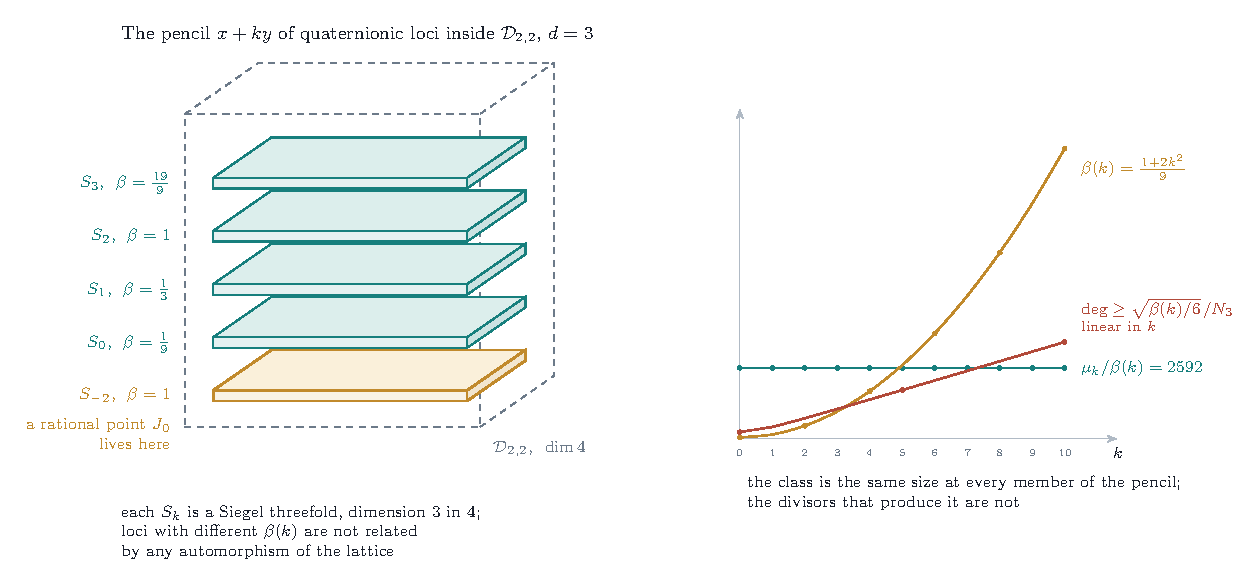
\includegraphics[width=\textwidth]{fig_pencil}
\caption{\Cref{prop:pencil} at $d=3$. Left: the members $S_{k}$ of the
pencil, each a Siegel threefold inside the four-dimensional family, with the
member $k=-2$, where $\beta=1$ and a rational point $J_{0}$ can be written
down, drawn apart. Right: along the pencil the ratio $\mu_{k}/\beta(k)$ is
the constant $2592$, so the Weil class is the same size at every member, while
the least degree of a divisor not proportional to $\eta$ grows linearly in
$k$. The class does not change; the divisors that produce it must.}
\label{fig:pencil}
\end{figure}

\begin{remark}[At $n=2$ the hypothesis is weaker still]\label{rem:ntwo}
Let $n=2$, so $\dim\cS=n^{2}=4$. The quaternionic locus of
\Cref{setup:quat} is the symmetric space of $\Sp(4,\RR)$ inside
$\cD_{2,2}$,\footnote{Left multiplication by the quaternion algebra
$B=(-d,b)$ commutes with $K$, and $B\otimes\RR\cong M_{2}(\RR)$ because
$b>0$, so Morita equivalence writes $V_{\RR}$ as $W\otimes_{\RR}\RR^{2}$ with
$W$ symplectic of dimension $2n$. The complex structures commuting with $B$
are then the complex structures on $W$, that is the points of the Siegel
space $\mathfrak{H}_{n}$, of dimension $n(n+1)/2$. The codimension in
$\cD_{n,n}$ is $n^{2}-n(n+1)/2=n(n-1)/2$, which is the count verified in
item (XII) of \Cref{sec:verification} for $n\le10$ and in
\texttt{quat\_locus\_codimension} of \Cref{sec:lean}.} of dimension
$n(n+1)/2=3$, so it is a divisor. Its $G(\QQ)$-translates are infinitely many
pairwise distinct irreducible closed subvarieties of $\cS$ of dimension $3$,
since a finite union of proper closed analytic subsets cannot be dense. If
infinitely many of them carry cycles with one and the same data
$(\underline{P},\underline{q})$, then the closed set
$\Sigma_{\underline{P},\underline{q}}$ has an irreducible component containing
infinitely many distinct irreducible threefolds, so that component has
dimension at least $4$ and therefore equals $\cS$. No density is needed at
$n=2$, only infinitude. Combined with the theorem of Moonen and Zarhin
\cite{MZ99} that every Hodge class on an abelian fourfold lies in the
subalgebra generated by divisor classes and Weil classes, the conclusion would
be the Hodge conjecture for all abelian fourfolds of Weil type, hence for all
abelian fourfolds. That conclusion is now Markman's theorem
\cite[Corollary 1.6.1]{Mar25a}, reached by a different route; at $n=2$ the
argument above would be a second proof, and it is at $n\ge3$ that it has
something to add.
\end{remark}

\subsubsection*{The second criterion: a rank at one point}

The other way to get from a dense algebraic locus to an open one is to make
the cycle move, and the classical tool for that is semiregularity. What
follows is not a new theorem about semiregularity; it is the observation that
after \Cref{thm:hdgcount}, \Cref{thm:everyfamily} and \Cref{thm:closedlocus},
the semiregularity of a single object at a single point implies the Hodge
conjecture for the whole family, with no further propagation argument. The
first step is that the object exists, and that its Chern character is as rigid
as it can be.

\begin{proposition}[The $K$-theory class at a base point]\label{prop:ktheory}
Let $s_{0}\in\Sigma$ be a base point of \Cref{thm:everyfamily} and write
$A_{0}=A_{s_{0}}$. There are an integer $N\ge1$ and a perfect complex $E$ on
$A_{0}$ with
\[
  \ch_{k}(E)=0\ \ (k\ne n),\qquad \ch_{n}(E)=N\,\omega_{1} .
\]
The tuple $v=\ch(E)$ extends to a flat section of
$\bigoplus_{k}R^{2k}f_{*}\QQ$ over $\cS$ which is of type $(k,k)$ at every
point.
\end{proposition}

\begin{proof}
By \Cref{thm:everyfamily} there is $\xi\in\CH^{n}(A_{0})_{\QQ}$ with
$\cl(\xi)=\omega_{1}$. For a smooth quasi-projective variety over a field the
Chern character $\ch\colon K_{0}(A_{0})_{\QQ}\to\CH^{*}(A_{0})_{\QQ}$ is a
ring isomorphism \cite[Ex.~15.2.16(b) and Cor.~18.3.2]{Ful98}, so there is a
unique $u\in K_{0}(A_{0})_{\QQ}$ with $\ch(u)=\xi$, and its Chern character
has no component outside degree $n$. Choose $N$ clearing the denominators of
$u$; then $Nu\in K_{0}(A_{0})$ is a difference of classes of vector bundles
and is therefore the class of a perfect complex $E$, with
$\ch(E)=N\xi$. Passing to cohomology gives the displayed identities.

For the last sentence, $\ch(E)$ has a single nonzero component, equal to
$N\omega_{1}$, and $\omega$ is a flat section of type $(n,n)$ everywhere by
\Cref{lem:omegadescends}.
\end{proof}

\begin{theorem}[Buchweitz and Flenner \cite{BF03}; Pridham \cite{Pri24}]\label{thm:BF}
Let $X$ be a smooth projective complex variety, $E$ a perfect complex on $X$,
and $X\hookrightarrow\cX\to\Spec R$ a deformation of $X$ over an Artin local
$\CC$-algebra along which $\ch(E)$ stays of Hodge type. If the semiregularity
map
\[
  \sigma_{E}\colon\Ext^{2}_{X}(E,E)
  \longrightarrow\bigoplus_{q\ge0}H^{q+2}(X,\Omega^{q}_{X}),
  \qquad
  \sigma_{E}(\zeta)=\sum_{q}\tfrac{1}{q!}\,
    \mathrm{tr}\bigl(\zeta\circ\mathrm{At}(E)^{q}\bigr),
\]
is injective, then $E$ extends to a perfect complex on $\cX$.
\end{theorem}

In this form, for perfect complexes and with every obstruction annihilated by
$\sigma_{E}$ and not only the curvilinear ones, the theorem is proved by
Pridham \cite{Pri24}, who identifies $\sigma_{E}$ with the tangent map of a
generalised Abel--Jacobi map on the derived moduli of perfect complexes; for
coherent sheaves see also \cite{BLM23}. Perry \cite{Per26} extends it to
noncommutative varieties with group actions, which covers twisted derived
categories and answers a question of Markman.

\begin{theorem}[Semiregularity at one point closes the family]
\label{thm:semiregclosure}
Let $n\ge2$, let $s_{0}$ and $E$ be as in \Cref{prop:ktheory}, and suppose the
semiregularity map $\sigma_{E}$ of \Cref{thm:BF} is
injective.\footnote{The hypothesis is not vacuous and it is not free, and the
degree-zero component shows both at once. For a line bundle $L$ one has
$\Ext^{2}(L,L)=H^{2}(\cO_{X})$ and $\sigma_{0}=\mathrm{tr}$ is the identity
on it, so $\sigma_{L}$ is injective for every line bundle on every variety,
and \Cref{thm:BF} returns the classical fact that a divisor class deforms
wherever it stays of type $(1,1)$. The object of \Cref{prop:ktheory} has rank
zero, so its trace component is not an isomorphism and in general not
injective, the source having no reason to be as small as
$h^{2}(\cO_{A_{0}})=\binom{2n}{2}$. The entire hypothesis therefore rests on
the components with $q\ge1$, which is exactly the range in which
semiregularity stops being formal and starts being a computation.} Then
$\Sigma=\cD_{n,n}$, and the Hodge conjecture holds in every degree for every
abelian $2n$-fold of $(K,-1,n)$-Weil type with $\Hg(A)=\SU(V,H)$ in that
family.
\end{theorem}

\begin{remark}[The hypothesis is not met by the object above]
\label{rem:semiregunavailable}
By \Cref{prop:concentrated} the complex of \Cref{prop:ktheory} has
$\dim\ker\sigma_{E}\ge n^{2}$ at every base point constructed in this paper,
so the hypothesis of \Cref{thm:semiregclosure} is not satisfied by it. The
theorem is stated because the hypothesis concerns a choice of perfect complex
representing a class in $K_{0}$, and a different representative is not
excluded; but no representative that is presently available satisfies it. See
\Cref{rem:killsreduction}, and \Cref{thm:p2forces} below for what any
representative satisfying it would have to look like.
\end{remark}

\begin{proof}
Let $\mathfrak{M}$ be the stack of perfect complexes with vanishing negative
self-extensions on the fibres of $f\colon\cA\to\cS$. It is algebraic and
locally of finite presentation over $\cS$ \cite{Lie06}, and at a point $[E]$
over $s_{0}$ its deformation theory relative to $\cS$ has tangent space
$\Ext^{1}(E,E)$ and obstruction space $\Ext^{2}(E,E)$. If
$\Ext^{<0}(E,E)\ne0$, which that stack excludes,\footnote{Lieblich's
stack parametrises the complexes he calls universally gluable, those with
$\Ext^{<0}(E,E)=0$; without that condition a complex can have automorphisms
of negative degree, and the natural moduli object is the derived stack of
To\"en and Vaqui\'e.} use instead the analytic Kuranishi germ of pairs of the
proof of \Cref{thm:p2false}, with the same tangent and obstruction spaces; the argument below then gives a nonempty
analytic open set in place of a Zariski open one, which is all that
\Cref{cor:allornothing} needs.

By \Cref{prop:ktheory} the Chern character of $E$ stays of Hodge type along
every direction in $\cS$, because it is a flat section of Hodge classes on the
whole base. So \Cref{thm:BF} applies to every infinitesimal deformation of
$A_{0}$ inside the family, and injectivity of $\sigma_{E}$ kills every
obstruction. The morphism $\mathfrak{M}\to\cS$ is therefore formally smooth at
$[E]$, and being locally of finite presentation it is smooth at $[E]$; in
particular it is dominant near $[E]$, so by Chevalley its image contains a
nonempty Zariski open $U\subseteq\cS$.

For $s\in U$ pick a perfect complex $E_{s}$ on $A_{s}$ in the fibre. Its
Chern character is $N\omega_{1}$ in degree $n$ and zero elsewhere, and Chern
characters of perfect complexes are algebraic, so $N\omega_{1}$ and hence
$\omega_{1}$ is algebraic on $A_{s}$; the rest of the Weil line follows by
\Cref{lem:onecomponent}. So $p^{-1}(U)\subseteq\Sigma$, which therefore
contains a nonempty open set, and \Cref{cor:allornothing} gives
$\Sigma=\cD_{n,n}$. Apply \Cref{thm:residual}(a).
\end{proof}

\subsubsection*{What the rank at one point forces}

The hypothesis of \Cref{thm:semiregclosure} is a rank, and a rank is not
open to inspection until the object is written down. It nevertheless has
consequences that can be stated for every representative at once, because the
semiregularity map composed with the evaluation map of Hochschild cohomology
is contraction into the Chern character (\Cref{setup:criterion}), and the
Chern character here is a Weil class. The annihilator of a Weil class in
$HT^{2}$ is large, and injectivity forces the evaluation map to vanish on the
whole of it. We compute the annihilator and draw the consequences; they are the
exact analogue, for (P2), of what \Cref{thm:candidatefails} and
\Cref{thm:nosplit} do for the secant route, and they use the same local
products.

\begin{theorem}[What injectivity of the semiregularity map forces]
\label{thm:p2forces}
Let $A$ be an abelian $2n$-fold of $(K,-1,n)$-Weil type, $n\ge2$, and write
$H^{1}(A,\CC)=V_{+}\oplus V_{-}$ for the eigenspaces of $K$,
$V_{\pm}^{1,0}$, $V_{\pm}^{0,1}$ for their Hodge components and
$T_{\pm}\subset H^{0}(T_{A})=T_{0}A$ for the eigenspaces of $K$ on the tangent
space, each of dimension $n$. Let $\omega=a\alpha_{+}+b\alpha_{-}$ be a
class on the Weil line with $ab\ne0$, for instance any nonzero rational one,
and let $E$ be a nonzero perfect complex on $A$ with $\ch(E)=N\omega$,
$N\ne0$, and no other component.
\begin{enumerate}[label=\textup{(\roman*)},leftmargin=2.6em,itemsep=2pt]
\item The annihilator of $\ch(E)$ in $HT^{2}(A)$ is
  \[
    \Ann_{HT^{2}}(\ch E)
    =\bigl(V_{+}^{0,1}\otimes V_{-}^{0,1}\bigr)
    \;\oplus\;\Hom_{K}\bigl(H^{1,0},H^{0,1}\bigr)
    \;\oplus\;\bigl(T_{+}\otimes T_{-}\bigr),
  \]
  of dimension $n^{2}+2n^{2}+n^{2}=4n^{2}$: the mixed block of $H^{0,2}$,
  which is the annihilator of \Cref{lem:annihilator}; the $K$-linear first
  order deformations of $A$, which contain the tangent space of the polarised
  Weil family; and the mixed bivectors.
\item If $\sigma_{E}$ is injective, then $\operatorname{ev}_{E}$ vanishes on
  this space. Explicitly: $z\cdot\id_{E}=0$ for every $z\in V_{+}^{0,1}\otimes
  V_{-}^{0,1}$; $E$ extends to first order along every $K$-linear deformation
  of $A$; and the translation classes satisfy $A_{\theta}A_{\theta'}=0$ in
  $\Ext^{2}(E,E)$ for every $\theta\in T_{+}$ and $\theta'\in T_{-}$.
\item Under the same hypothesis the algebra map $H^{*}(\cO_{A})\to\Ext^{*}(E,E)$,
  $z\mapsto z\cdot\id_{E}$, kills the ideal generated by the mixed block,
  which is $\bigoplus_{a,b\ge1}\bigwedge^{a}V_{+}^{0,1}\otimes\bigwedge^{b}V_{-}^{0,1}$;
  so the image of $H^{0,k}(A)$ has dimension at most $2\binom{n}{k}$ for
  $1\le k\le n$ and is zero for $k>n$, and every endomorphism $f$ of $E$ has
  $\operatorname{tr}(f)=0$ in $H^{0}(\cO_{A})=\CC$.
\item Under the same hypothesis, if at some point $p$ of its support $E$ is
  locally isomorphic to $i_{*}F$ with $F$ locally free of positive rank on a
  smooth closed subvariety $Z\ni p$ of codimension at least two, then
  $T_{+}\subseteq T_{p}Z$ or $T_{-}\subseteq T_{p}Z$.
\end{enumerate}
\end{theorem}

\begin{proof}
(i) Write $H^{*}(A,\CC)=\bigwedge^{*}(H^{1,0}\oplus H^{0,1})$ and
$\alpha_{\pm}$ for a generator of $\bigwedge^{2n}V_{\pm}
=\bigwedge^{n}V_{\pm}^{1,0}\otimes\bigwedge^{n}V_{\pm}^{0,1}$. The three
summands of $HT^{2}$ act as follows: $z\in H^{0,2}=\bigwedge^{2}H^{0,1}$ by
wedge product; $v\in H^{1}(T_{A})=\Hom(H^{1,0},H^{0,1})$ as the derivation
that replaces one $(1,0)$ factor by its image; $\pi\in H^{0}(\bigwedge^{2}T_{A})
=\bigwedge^{2}(H^{1,0})^{\vee}$ by double contraction of $(1,0)$ factors. For
$z$, the computation is \Cref{lem:annihilator}. For $v$, decompose
$\Hom(H^{1,0},H^{0,1})$ into its four blocks by eigenspaces. A block
$\Hom(V_{+}^{1,0},V_{+}^{0,1})$ replaces a factor of $\bigwedge^{n}V_{+}^{1,0}$
in $\alpha_{+}$ by an element of $V_{+}^{0,1}$, which is already exhausted in
$\alpha_{+}$, so it kills $\alpha_{+}$; it acts trivially on $\alpha_{-}$,
which has no $V_{+}^{1,0}$ factor. Likewise $\Hom(V_{-}^{1,0},V_{-}^{0,1})$
kills $\omega$. The block $\Hom(V_{+}^{1,0},V_{-}^{0,1})$ carries $\alpha_{+}$
to a nonzero element of $\bigwedge^{n-1}V_{+}^{1,0}\otimes V_{-}^{0,1}
\otimes\bigwedge^{n}V_{+}^{0,1}$ and kills $\alpha_{-}$, and
$\Hom(V_{-}^{1,0},V_{+}^{0,1})$ carries $\alpha_{-}$ to a nonzero element of
a different summand of $H^{n-1,n+1}$; since $ab\ne0$ and the two summands are
independent, a general $v$ kills $\omega$ if and only if its two mixed blocks
vanish, that is, if and only if $v$ is $K$-linear. The space of $K$-linear
maps has dimension $2n^{2}$, and it contains the $n^{2}$-dimensional tangent
space of the polarised family, which is its symmetric part. For $\pi$, a
mixed bivector $\theta\wedge\theta'$ with $\theta\in T_{+}=(V_{+}^{1,0})^{\vee}$
and $\theta'\in T_{-}=(V_{-}^{1,0})^{\vee}$ kills $\alpha_{+}$ because
$\theta'$ kills every factor of $\bigwedge^{n}V_{+}^{1,0}$, and kills
$\alpha_{-}$ symmetrically; a bivector in $\bigwedge^{2}T_{+}$ carries
$\alpha_{+}$ to a nonzero element of $\bigwedge^{n-2}V_{+}^{1,0}
\otimes\bigwedge^{n}V_{+}^{0,1}$ and kills $\alpha_{-}$, and symmetrically
for $\bigwedge^{2}T_{-}$. Since the images of the three summands of $HT^{2}$
lie in the three different Hodge components $H^{n,n+2}$, $H^{n-1,n+1}$ and
$H^{n-2,n}$ of $H^{2n+2}(A,\CC)$, the annihilator is the direct sum of the
three annihilators computed, of dimensions $n^{2}$, $2n^{2}$ and $n^{2}$. Item
(XXXV) of \Cref{sec:verification} carries out the whole computation in the
exterior algebra for $n=2$ and $n=3$.

(ii) By the commutative square $\sigma_{E}\circ\operatorname{ev}_{E}
=(\,\cdot\,)\lrcorner\ch(E)$ of \Cref{setup:criterion}, $\sigma_{E}$
vanishes on $\operatorname{ev}_{E}(\Ann_{HT^{2}}(\ch E))$; if $\sigma_{E}$
is injective, $\operatorname{ev}_{E}$ vanishes there. The three explicit
statements are \eqref{eq:evgeneral} on the three summands of (i): on
$H^{0,2}$ the evaluation map is $z\mapsto z\cdot\id_{E}$; on $H^{1}(T_{A})$
it is the obstruction map $v\mapsto v\lrcorner\mathrm{At}(E)$, whose
vanishing on $v$ is the extension of $E$ to first order along $v$
\cite{Tod09}; and on a bivector $\theta\wedge\theta'$ it is
$\tfrac12(\theta\wedge\theta')\lrcorner\mathrm{At}(E)^{2}
=A_{\theta}A_{\theta'}$, as in the proof of \Cref{thm:candidatefails}.

(iii) The map $z\mapsto z\cdot\id_{E}$ is a homomorphism of graded algebras
from $H^{*}(\cO_{A})=\bigwedge^{*}H^{0,1}$ to the Yoneda algebra, because the
classes from $H^{*}(A,\CC)$ are graded central there, so its kernel is an
ideal, and by (ii) it contains the mixed block $V_{+}^{0,1}\otimes V_{-}^{0,1}$.
The ideal generated by the mixed block in $\bigwedge^{*}(V_{+}^{0,1}\oplus
V_{-}^{0,1})=\bigwedge^{*}V_{+}^{0,1}\otimes\bigwedge^{*}V_{-}^{0,1}$ is the
sum of the summands $\bigwedge^{a}V_{+}^{0,1}\otimes\bigwedge^{b}V_{-}^{0,1}$
with $a,b\ge1$, since each such summand is a multiple of the mixed block and
the remaining summands, $a=0$ or $b=0$, meet the ideal in zero; the quotient in
degree $k\ge1$ is $\bigwedge^{k}V_{+}^{0,1}\oplus\bigwedge^{k}V_{-}^{0,1}$,
of dimension $2\binom{n}{k}$, and zero for $k>n$. In particular the top class
of $H^{2n}(\cO_{A})$, which is mixed for $n\ge1$, acts by zero. Serre duality
on $A$, whose canonical bundle is trivial, is the perfect pairing
$\Ext^{2n}(E,E)\times\Hom(E,E)\to H^{2n}(\cO_{A})\cong\CC$,
$(\xi,f)\mapsto\operatorname{tr}(\xi\circ f)$; for $\xi=w\cdot\id_{E}$
with $w$ the top class this is $w\cdot\operatorname{tr}(f)$, where
$\operatorname{tr}(f)\in H^{0}(\cO_{A})=\CC$, so $w\cdot\id_{E}=0$ forces
$\operatorname{tr}(f)=0$ for every $f$.

(iv) Let $\cO$ be the local ring of $A$ at $p$ and choose coordinates with
$Z=\{x_{1}=\dots=x_{c}=0\}$, $c\ge2$. Locally $E\cong(\cO/J)^{\oplus r}$
with $J=(x_{1},\dots,x_{c})$, a regular sequence, so
$\Ext^{*}_{\cO}(\cO/J,\cO/J)=\bigwedge^{*}_{\cO/J}N$ as a graded algebra,
where $N=\Hom(J/J^{2},\cO/J)$ is the normal module with basis the classes
$\partial_{1},\dots,\partial_{c}$ dual to $x_{1},\dots,x_{c}$; the
$\Ext^{1}$ is computed on the Koszul resolution exactly as in the proof of
\Cref{lem:localproducts}, and the product is the wedge because the Yoneda
algebra of a Koszul complex is the exterior algebra on the dual of the
generators. For $E$ of rank $r$ the local Yoneda algebra is
$\bigwedge^{*}N\otimes M_{r}(\cO/J)$. By \Cref{lem:edge} the germ of
$A_{\theta}$ at $p$ is the jet class along $\theta$; on the Koszul complex the
jet class of a derivation $D$ is the chain map $-D(d)$, and for
$D=\theta=\sum_{i}c^{i}\partial_{i}$ its component in $\Ext^{1}=N\otimes M_{r}(\cO/J)$
is $\sum_{i\le c}(c^{i}\bmod J)\,\partial_{i}\otimes\id$, the class of
$\theta$ modulo $T_{Z}$. Multiplicativity of the germ map then gives the germ
of $A_{\theta}A_{\theta'}$ as
$(\theta\bmod T_{Z})\wedge(\theta'\bmod T_{Z})\otimes\id$ in
$\bigwedge^{2}N\otimes M_{r}(\cO/J)$, whose value at $p$ is
$\bar\theta(p)\wedge\bar\theta'(p)\in\bigwedge^{2}(T_{p}A/T_{p}Z)$. If
$A_{\theta}A_{\theta'}=0$ for all $\theta\in T_{+}$, $\theta'\in T_{-}$,
then $\bar a\wedge\bar b=0$ for all $\bar a$ in the image $I_{+}$ of $T_{+}$
and $\bar b$ in the image $I_{-}$ of $T_{-}$ in $N_{p}=T_{p}A/T_{p}Z$, and
$I_{+}+I_{-}=N_{p}$ since $T_{+}\oplus T_{-}=T_{p}A$. If both $I_{\pm}$ were
nonzero, every nonzero $\bar b\in I_{-}$ would be proportional to every
nonzero $\bar a\in I_{+}$, so $I_{+}=I_{-}$ would be a line and
$N_{p}=I_{+}+I_{-}$ of dimension one, against $c\ge2$. Hence $I_{+}=0$ or
$I_{-}=0$, which is the claim. The two pieces of linear algebra, the shape of
the ideal in (iii) and the dichotomy just used, are checked in item (XXXV).
\end{proof}

\begin{corollary}[Where (P2) can and cannot be met]\label{cor:p2shape}
Let $A$ be as in \Cref{thm:p2forces} and suppose that no proper abelian
subvariety $B\subset A$ has $T_{0}B\supseteq T_{+}$ or $T_{0}B\supseteq T_{-}$;
equivalently, that $A$ has no $K$-stable abelian subvariety on which $K$ acts
through a single embedding, which holds whenever $A$ is simple, at every
split member $X\times\widehat X$ with $X$ simple of endomorphism algebra
$\QQ$, and at a general point of the quaternionic locus of \Cref{setup:quat}.
Let $E$ be a perfect complex on $A$ with $\ch(E)=N\omega$ as above and
$\sigma_{E}$ injective. Then no irreducible component $Z_{0}$ of the support
of $E$ of codimension at least two has a dense open subset along which $E$ is
a locally free sheaf of positive rank on $Z_{0}$. In particular $E$ is not a
sheaf, and along every component of its support of codimension at least two
it has, generically, either at least two nonvanishing cohomology sheaves or a
cohomology sheaf that is not locally free on the reduced support.
\end{corollary}

\begin{proof}
Suppose $Z_{0}$ is such a component, with $U\subseteq Z_{0}^{\mathrm{sm}}$ dense
open and $E|_{U}$ a locally free sheaf of positive rank on $U$. By
\Cref{thm:p2forces}(iv), $U=U_{+}\cup U_{-}$ with
$U_{\pm}=\{p\in U:T_{\pm}\subseteq T_{p}Z_{0}\}$, both closed in $U$; as $U$
is irreducible, $U=U_{+}$ say. Then every constant vector field
$\theta\in T_{+}$ is tangent to $Z_{0}$ along $U$, hence along
$Z_{0}^{\mathrm{sm}}$. The set
$S=\{(p,t)\in Z_{0}\times\CC:p+\exp(t\theta)\in Z_{0}\}$ is a closed
analytic subset of the irreducible space $Z_{0}\times\CC$, and it contains
an open neighbourhood of $Z_{0}^{\mathrm{sm}}\times\{0\}$, because the local
flow of the restriction of $\theta$ to the submanifold $Z_{0}^{\mathrm{sm}}$
exists on such a neighbourhood; so $S=Z_{0}\times\CC$, and
$Z_{0}+\exp(t\theta)\subseteq Z_{0}$, hence $=Z_{0}$, for every $t$. Let
$G=\{x\in A:Z_{0}+x=Z_{0}\}$, a closed algebraic subgroup of $A$, and $B$
its identity component, an abelian subvariety. The connected set
$\exp(T_{+})$ contains $0$ and lies in $G$, hence in $B$, so
$T_{+}\subseteq T_{0}B$. By hypothesis $B=A$, so $Z_{0}=A$, against the
codimension. If $E$ were a sheaf, its support would have codimension exactly
$n\ge2$ and along a dense open set of every component it would be locally
free of positive rank on the reduced support, which is excluded; the last
sentence is the negation of the same condition.

For the equivalence in the hypothesis, let $\sqrt{-d}$ act on $A$ through
an order of $K$. If $B\ne A$ has $T_{0}B\supseteq T_{+}$, then
$H_{1}(B,\QQ)\cap\sqrt{-d}\,H_{1}(B,\QQ)$ is a $K$-stable sub-Hodge
structure, hence $H_{1}(C,\QQ)$ for a $K$-stable abelian subvariety
$C\subseteq B$, and its real points $T_{0}B\cap\sqrt{-d}\,T_{0}B$ still
contain $T_{+}$, on which $\sqrt{-d}$ acts by a scalar. The $K$-stable
complement $C'$ of $C$ for the polarisation is nonzero, since $C\subseteq B\ne A$,
and $T_{0}C'$ is a $K$-stable complement of $T_{0}C\supseteq T_{+}$, so
$T_{0}C'\subseteq T_{-}$ and $K$ acts on $C'$ through a single embedding.
Conversely, if a nonzero $K$-stable $C'\ne A$ has $T_{0}C'\subseteq T_{-}$,
its $K$-stable complement $B$ is proper with $T_{0}B\supseteq T_{+}$. For the
three cases: a simple $A$ has no proper abelian subvariety; for
$X\times\widehat X$ with $X$ simple and $\End^{0}(X)=\QQ$ the sub-Hodge
structures of $H_{1}(X)\otimes\QQ^{2}$ are $H_{1}(X)\otimes W$ with
$W\subseteq\QQ^{2}$, and $W$ is $K$-stable only for $W=0$ or $\QQ^{2}$, $K$
acting on $\QQ^{2}$ through a quadratic field; and at a general quaternionic
member $A$ is either simple or, when the quaternion algebra of
\Cref{setup:quat} splits, isogenous to $C\times C$ with $C$ a general
principally polarised abelian $n$-fold, whose sub-Hodge structures are again
$H_{1}(C)\otimes W$ with the same conclusion.
\end{proof}

\subsubsection*{The whole Hochschild action, and the two branches}

\Cref{thm:p2forces} computes the annihilator degree by degree and reads off
what the vanishing of the evaluation map on it means for $E$. The annihilator
has a structure that the degree-by-degree description hides, and bringing it
out costs nothing and gives more: it is the mixed part of a splitting of
$HH^{1}(A)$ into two halves, one for each of the two conjugate pieces of the
Weil class. Everything in this subsection is about the Hochschild cohomology
of $A$ alone, and the consequences for $E$ follow from it formally.

\begin{setupenv}[Hochschild cohomology in these terms]\label{setup:hh}
For an abelian variety $A$ the Hochschild--Kostant--Rosenberg isomorphism
identifies
\[
  HH^{*}(A)\;\cong\;HT^{*}(A)=\bigoplus_{p,q}H^{p}\bigl(\textstyle\bigwedge^{q}T_{A}\bigr)
  =\textstyle\bigwedge^{*}\bigl(H^{0,1}(A)\oplus H^{0}(T_{A})\bigr),
\]
as a graded ring, the grading being $p+q$; the Todd class of $A$ is trivial,
so the twist by $\td^{1/2}$ in \cite{Cal05}, \cite{CRV12} is the identity and
the identification is a ring isomorphism on the nose. Write
$HH^{1}(A)=H^{0,1}(A)\oplus H^{0}(T_{A})$, of dimension $4n$, so that
$HH^{*}(A)$ is the exterior algebra on it, of dimension $2^{4n}$. It acts on
$H^{*}(A,\CC)=\bigwedge^{*}\bigl(H^{1,0}\oplus H^{0,1}\bigr)$ by wedging with
the classes of $H^{0,1}$ and contracting the classes of $H^{1,0}$ against
$H^{0}(T_{A})$; the two families of operators involve disjoint generators, so
they pairwise anticommute and the action is an action of the exterior algebra.
In degree two this is the operator $x\lrcorner$ of \Cref{setup:criterion}, and
$\operatorname{ev}_{E}\colon HH^{*}(A)\to\Ext^{*}(E,E)$ is a homomorphism of
graded rings into the graded centre, with
$\sigma_{E}\circ\operatorname{ev}_{E}=(\,\cdot\,)\lrcorner\ch(E)$
\cite[Section 6]{BF08}, \cite{Cal05}, \cite{CRV12}.
\end{setupenv}

\begin{theorem}[The annihilator is the mixed part of a splitting]
\label{thm:hhsplitting}
Let $A$ be of $(K,-1,n)$-Weil type with $n\ge2$, and let
$\omega=a\alpha_{+}+b\alpha_{-}$ lie on the Weil line with $ab\ne0$. Put
\[
  P=\Ann_{HH^{1}}(\alpha_{+})=V_{+}^{0,1}\oplus T_{-},
  \qquad
  Q=\Ann_{HH^{1}}(\alpha_{-})=V_{-}^{0,1}\oplus T_{+} .
\]
\begin{enumerate}[label=\textup{(\roman*)},leftmargin=2.6em,itemsep=2pt]
\item $\dim P=\dim Q=2n$ and $HH^{1}(A)=P\oplus Q$; in particular
  $\Ann_{HH^{1}}(\omega)=0$.
\item $\Ann_{HH^{2}}(\omega)=P\wedge Q$, of dimension $4n^{2}$. This is the
  space computed in \Cref{thm:p2forces}(i), written as the mixed part of the
  splitting.
\item Contraction with $\alpha_{-}$ is injective on $\bigwedge^{*}P$, and
  contraction with $\alpha_{+}$ is injective on $\bigwedge^{*}Q$; the two
  images meet in exactly one line, in degree $2n$.
\item For every $k\ge1$,
  \[
    \Ann_{HH^{k}}(\omega)
    =\Bigl(\bigoplus_{\substack{i+j=k\\ i,j\ge1}}
      \textstyle\bigwedge^{i}P\wedge\bigwedge^{j}Q\Bigr)\;\oplus\;\epsilon_{k},
  \]
  where $\epsilon_{k}=0$ for $k\ne2n$ and $\epsilon_{2n}$ is the line of
  \textup{(iii)}. So
  $\dim\Ann_{HH^{k}}(\omega)=\binom{4n}{k}-2\binom{2n}{k}+\delta_{k,2n}$ for
  $k\ge1$, while $\Ann_{HH^{0}}(\omega)=0$, and the annihilator is the ideal
  generated by its degree-two part together with that one line.
\end{enumerate}
\end{theorem}

\begin{proof}
Choose bases $x_{1},\dots,x_{n}$ of $V_{+}^{1,0}$ and $y_{1},\dots,y_{n}$ of
$V_{-}^{1,0}$, and bases $\bbar x_{i}$ of $V_{+}^{0,1}$ and $\bbar y_{j}$ of
$V_{-}^{0,1}$ (the bar is notation only: complex conjugation carries
$V_{+}^{1,0}$ to $V_{-}^{0,1}$), so that $\alpha_{+}=x_{1}\cdots x_{n}\bbar x_{1}\cdots\bbar x_{n}$
and $\alpha_{-}=y_{1}\cdots y_{n}\bbar y_{1}\cdots\bbar y_{n}$, and write
$\partial_{x_{i}},\partial_{y_{j}}$ for the dual basis of
$H^{0}(T_{A})=T_{+}\oplus T_{-}$.

(i) Of the $4n$ basis operators, $\bbar x_{i}\wedge$ kills $\alpha_{+}$
because $\bbar x_{i}$ already occurs in it, and $\partial_{y_{j}}\lrcorner$
kills $\alpha_{+}$ because no $y$ occurs in it; so $P\supseteq
V_{+}^{0,1}\oplus T_{-}$. Conversely $\bbar y_{j}\wedge\alpha_{+}\ne0$ and
$\partial_{x_{i}}\lrcorner\alpha_{+}\ne0$, and these images lie in different
summands of $H^{*}$, so no nonzero combination of them kills $\alpha_{+}$:
$P=V_{+}^{0,1}\oplus T_{-}$, of dimension $2n$. The computation for $Q$ is the
same with the roles of the two eigenspaces exchanged, and
$P\cap Q=0$ with $\dim P+\dim Q=4n$, so $HH^{1}=P\oplus Q$. A class killing
$\omega$ in degree one kills $\alpha_{+}$ and $\alpha_{-}$ separately, the two
images lying in different summands and $ab\ne0$, so it lies in $P\cap Q=0$.

(iii) A monomial $\bbar x_{I}\partial_{y_{J}}\in\bigwedge^{*}P$ contracts
$\alpha_{-}$ to $\pm\,\bbar x_{I}\,y_{[n]\setminus J}\,\bbar y_{[n]}$, and
these are linearly independent for distinct pairs $(I,J)$, which is the
injectivity; the statement for $Q$ is symmetric. For the intersection, the
image of $\bigwedge^{*}P$ consists of classes with no $x$ and at most $n$
factors $\bbar x$, and the image of $\bigwedge^{*}Q$ of classes with $n$
factors $\bbar x$ and $n-\#\{\partial_{x}\}$ factors $x$. A common class
therefore has no $x$ and all $n$ factors $\bbar x$ and, by the same count in
the other eigenspace, no $y$ and all $n$ factors $\bbar y$: it is a multiple
of $\bbar x_{[n]}\bbar y_{[n]}$, and it comes from
$\pi_{P}=\bbar x_{[n]}\partial_{y_{[n]}}$ and
$\pi_{Q}=\bbar y_{[n]}\partial_{x_{[n]}}$, both of degree $2n$. So the
intersection is the single line spanned by that class.

(ii) and (iv) Decompose $\bigwedge^{k}HH^{1}=\bigoplus_{i+j=k}\bigwedge^{i}P
\wedge\bigwedge^{j}Q$. A summand with $i,j\ge1$ annihilates $\alpha_{+}$,
because it has a factor in $P$ and the action is by an algebra, and
annihilates $\alpha_{-}$ for the same reason with $Q$; so it lies in the
annihilator of $\omega$. On the remaining two summands, $\xi_{P}\in\bigwedge^{k}P$
has $\xi_{P}\lrcorner\omega=b\,\xi_{P}\lrcorner\alpha_{-}$ and
$\xi_{Q}\in\bigwedge^{k}Q$ has $\xi_{Q}\lrcorner\omega=a\,\xi_{Q}\lrcorner\alpha_{+}$,
so by (iii) a combination $\xi_{P}+\xi_{Q}$ annihilates $\omega$ if and only
if $b\,\xi_{P}\lrcorner\alpha_{-}=-a\,\xi_{Q}\lrcorner\alpha_{+}$, which by
(iii) happens only for $k=2n$ and then only on the line
$b^{-1}\pi_{P}-a^{-1}\pi_{Q}$ up to scale. Taking $k=2$ and $n\ge2$, so that
$2\ne2n$, gives (ii), the dimension being
$\dim P\cdot\dim Q=4n^{2}$; the general count is
$\binom{4n}{k}-\binom{2n}{k}-\binom{2n}{k}$ plus the exceptional line. Item
(XXXVIII) of \Cref{sec:verification} carries out the whole computation in the
exterior algebra over $\QQ$ for $n=1$ and $n=2$ in every degree, for two
choices of $(a,b)$, and for $n=3$ in degrees up to three.
\end{proof}

\begin{corollary}[What the criterion forces on the Hochschild action]
\label{cor:hhfactor}
Let $A$ and $\omega$ be as above and let $E$ be a nonzero perfect complex on
$A$ with $\ch(E)=N\omega$, $N\ne0$.
\begin{enumerate}[label=\textup{(\roman*)},leftmargin=2.6em,itemsep=2pt]
\item Unconditionally, $\dim\Ext^{2}(E,E)\ge2n(2n-1)$.
\item If $\sigma_{E}$ is injective then $\operatorname{ev}_{E}$ vanishes on
  $P\wedge Q$, hence on the ideal it generates, and the ring homomorphism
  $\operatorname{ev}_{E}\colon HH^{*}(A)\to\Ext^{*}(E,E)$ factors through
  \[
    R\;=\;\textstyle\bigwedge^{*}P\;\oplus_{\CC}\;\bigwedge^{*}Q,
    \qquad \dim_{\CC}R=2^{2n+1}-1,
  \]
  the two exterior algebras glued along their scalars, inside $HH^{*}(A)$ of
  dimension $2^{4n}$. At $n=2$ that is $31$ out of $256$.
\item Granting the compatibility
  $\sigma_{E}\circ\operatorname{ev}_{E}=(\,\cdot\,)\lrcorner\ch(E)$ in degree
  $k$ \cite{Cal05}, \cite{CRV12}, the induced map on $R$ is injective away
  from the line of \Cref{thm:hhsplitting}(iii), so
  \[
    \dim\Ext^{k}(E,E)\;\ge\;2\binom{2n}{k}\quad(1\le k<2n),
    \qquad
    \sum_{k\ge1}\dim\Ext^{k}(E,E)\;\ge\;2^{2n+1}-3 .
  \]
\end{enumerate}
\end{corollary}

\begin{proof}
(i) By \Cref{setup:hh}, $\ker\operatorname{ev}_{E}\subseteq\Ann_{HH^{2}}(\ch E)$
in degree two, since $\sigma_{E}(\operatorname{ev}_{E}(\xi))=\xi\lrcorner\ch(E)$
and the right side is nonzero off the annihilator. Hence
$\dim\Ext^{2}(E,E)\ge\dim HH^{2}(A)-\dim\Ann_{HH^{2}}(\omega)
=\binom{4n}{2}-4n^{2}=2n(2n-1)$ by \Cref{thm:hhsplitting}(ii). No hypothesis
on $\sigma_{E}$ is used.

(ii) $\operatorname{ev}_{E}$ vanishes on the annihilator by
\Cref{thm:p2forces}(ii), its kernel is an ideal because it is a ring map, and
the ideal generated by $P\wedge Q$ in $\bigwedge^{*}(P\oplus Q)
=\bigwedge^{*}P\otimes\bigwedge^{*}Q$ is the sum of the summands with
$i,j\ge1$, whose complement is $\bigwedge^{*}P\oplus_{\CC}\bigwedge^{*}Q$ of
dimension $2\cdot2^{2n}-1$.

(iii) With the compatibility in degree $k$, the argument of (i) gives
$\ker\operatorname{ev}_{E}\subseteq\Ann_{HH^{k}}(\omega)$, and by
\Cref{thm:hhsplitting}(iv) that annihilator meets $\bigwedge^{k}P\oplus
\bigwedge^{k}Q$ only in the exceptional line. So the map induced on $R$ has
kernel contained in that one line and its image has dimension at least
$\dim R-1=2^{2n+1}-2$. One of those dimensions sits in degree zero, where the
image is $\CC\cdot\id_{E}$, nonzero because $E$ is; the rest is distributed
over the positive degrees, which is the second display, and in degree $k$ the
image contains the $2\binom{2n}{k}$ dimensions of
$\bigwedge^{k}P\oplus\bigwedge^{k}Q$ for $k<2n$, which is the first.
\end{proof}

\begin{remark}[The two branches, and what they are not]\label{rem:twobranches}
The ring $R$ of \Cref{cor:hhfactor}(ii) is the ring of functions on two odd
affine spaces of dimension $2n$ crossing at the origin. Read that way, the
statement is that if $E$ satisfies the criterion then the deformations of
$D^{b}(A)$ along which its Hochschild action survives form two branches, $P$
and $Q$, meeting only at the trivial deformation; and the two branches are the
annihilators of the two conjugate pieces $\alpha_{+}$ and $\alpha_{-}$ of the
Weil class. The criterion says that $E$ sees the two halves of the class
separately and their interaction not at all.

Two things this is not. The splitting $HH^{1}=P\oplus Q$ is not the splitting
into eigenspaces of $K$: the eigenspaces are
$V_{+}^{0,1}\oplus T_{+}$ and $V_{-}^{0,1}\oplus T_{-}$, and $P$ and $Q$ cross
them. It is the splitting into the annihilators of $\alpha_{+}$ and of
$\alpha_{-}$, and it exists because the Weil class is a sum of two pieces each
of which is a top form on an eigenspace. And the conclusion is not a
contradiction: $R$ is a perfectly good ring, the bound of (iii) is consistent
with $\chi(E,E)$ computed in \Cref{prop:objectsize}, since
$\sum_{k}(-1)^{k}2\binom{2n}{k}=0$, and nothing here forbids an $E$ of the
required shape. What the corollary does is say how large such an $E$ must be
and how little of the Hochschild cohomology it may see. We have not
constructed one, and we do not claim that one exists.
\end{remark}

\subsubsection*{The criterion as a dimension, and where the object can live}

The same square gives two more things, and between them they change what one
would look for. The first converts the rank of $\sigma_{E}$ into a single
dimension, which is the form in which a candidate can actually be tested. The
second says where the support of $E$ may lie, and it excludes the place where
anyone would look first, namely a cycle representing the Weil class.

\begin{theorem}[The criterion is a dimension]\label{thm:p2numerical}
Let $A$, $\omega$ and $E$ be as in \Cref{cor:hhfactor}, so that
$\ch(E)=N\omega$ with $N\ne0$ and no other component.
\begin{enumerate}[label=\textup{(\roman*)},leftmargin=2.6em,itemsep=2pt]
\item If $\dim\Ext^{2}(E,E)=2n(2n-1)$, the least value that
  \Cref{cor:hhfactor}(i) allows, then $\operatorname{ev}_{E}\colon
  HH^{2}(A)\to\Ext^{2}(E,E)$ is surjective with kernel exactly $P\wedge Q$,
  the map $\sigma_{E}$ is injective, and every class of $\Ext^{2}(E,E)$ is a
  sum of products $\operatorname{ev}_{E}(p)\operatorname{ev}_{E}(p')
  +\operatorname{ev}_{E}(q)\operatorname{ev}_{E}(q')$ with $p,p'\in P$ and
  $q,q'\in Q$, hence lies in the graded centre of $\Ext^{*}(E,E)$.
\item Conversely, if $\sigma_{E}$ is injective, then
  $\operatorname{ev}_{E}(HH^{2}(A))$ has dimension exactly $2n(2n-1)$, and
  $\sigma_{E}$ carries it isomorphically onto $HH^{2}(A)\lrcorner\,\omega$.
\item Consequently, if at one base point $s_{0}$ of a family some perfect
  complex $E$ with $\ch(E)=N\omega_{1}$ has $\dim\Ext^{2}(E,E)=2n(2n-1)$,
  then $\Sigma=\cD_{n,n}$, and the Hodge conjecture holds in every degree for
  every member of that family with $\Hg(A)=\SU(V,H)$.
\end{enumerate}
\end{theorem}

\begin{proof}
(i) The square of \Cref{setup:hh} gives $\ker\operatorname{ev}_{E}
\subseteq\Ann_{HH^{2}}(\omega)=P\wedge Q$ in degree two, the equality being
\Cref{thm:hhsplitting}(ii). Hence $\operatorname{rank}\operatorname{ev}_{E}
\ge\binom{4n}{2}-4n^{2}=2n(2n-1)=\dim\Ext^{2}(E,E)$, so
$\operatorname{ev}_{E}$ is onto and its kernel, of dimension $4n^{2}$ and
contained in $P\wedge Q$, is all of $P\wedge Q$. Every class of
$\Ext^{2}(E,E)$ is then $\operatorname{ev}_{E}(\xi)$ for some $\xi$, and
$\sigma_{E}(\operatorname{ev}_{E}(\xi))=\xi\lrcorner\,\omega$ vanishes only for
$\xi\in P\wedge Q=\ker\operatorname{ev}_{E}$; so $\sigma_{E}$ is injective.
Since $HH^{2}(A)=\bigwedge^{2}P\oplus(P\wedge Q)\oplus\bigwedge^{2}Q$ and
$\operatorname{ev}_{E}$ is a ring map into the graded centre, the image is
$\operatorname{ev}_{E}(\bigwedge^{2}P)+\operatorname{ev}_{E}(\bigwedge^{2}Q)$,
which is the description of the classes.

(ii) By \Cref{thm:p2forces}(ii) the kernel of $\operatorname{ev}_{E}$ in
degree two contains $P\wedge Q$, and by the argument of (i) it is contained in
it, so it equals $P\wedge Q$ and the image has dimension $2n(2n-1)$. On that
image $\sigma_{E}\circ\operatorname{ev}_{E}$ is contraction into $\omega$,
whose kernel is exactly $P\wedge Q$, so $\sigma_{E}$ maps the image
isomorphically onto $HH^{2}(A)\lrcorner\,\omega$.

(iii) By (i) the map $\sigma_{E}$ is injective, and \Cref{thm:semiregclosure}
applies.
\end{proof}

\Cref{thm:p2numerical}(iii) is a sufficient condition for
$\mathbf{W}(K,n,\delta)$ that mentions no map at all: one object, at one
point, and one number.%
\footnote{The dimension of $\Ext^{2}(E,E)$ is computable in a way the rank of
$\sigma_{E}$ is not. For a complex built from sheaves whose cohomology is
known, the local to global spectral sequence
$E_{2}^{p,q}=H^{p}(A,\cE xt^{q}(E,E))\Rightarrow\Ext^{p+q}(E,E)$ reduces the
count to the cohomology of the local $\cE xt$ sheaves, and on an abelian
variety the cohomology of a sheaf supported on an abelian subvariety, or of a
homogeneous bundle, is a question of linear algebra. The rank of $\sigma_{E}$,
by contrast, requires the trace of the exponential of the Atiyah class on
every class of $\Ext^{2}$, which is a computation with the object and not only
with its invariants.}
At $n=2$ the number is $12$, at $n=3$ it is $30$, and the two computations
behind it are item (XXXIX) of \Cref{sec:verification}. Part (ii) says that
nothing is lost in reading the criterion this way on the central part of
$\Ext^{2}$; whether an injective $\sigma_{E}$ forces the whole of
$\Ext^{2}(E,E)$ to be central is a statement about $\Ext^{2n-2}$, by Serre
duality, which the square in degree two does not reach, and nothing below
uses it.

The second consequence rests on a local fact about complexes supported at a
point, which we state and prove first.

\begin{lemma}[Two jet classes on a complex of finite length]
\label{lem:finiteproduct}
Let $R=\CC[[x_{1},\dots,x_{c}]]$ with $c\ge2$, let $M$ be a bounded complex of
finitely generated free $R$-modules whose cohomology has finite length, and
put $\chi(M)=\sum_{i}(-1)^{i}\ell(H^{i}(M))$. For $a\in\CC^{c}$ let
$J(a)\in\Ext^{1}_{R}(M,M)$ be the jet class of $M$ along the constant vector
field $\sum_{i}a_{i}\partial_{i}$, represented by the chain map
$-\sum_{i}a_{i}\partial_{i}(d)$ as in the proof of \Cref{thm:p2forces}(iv).
If $\chi(M)\ne0$ and $a,b$ are linearly independent, then $J(a)J(b)\ne0$ in
$\Ext^{2}_{R}(M,M)$.
\end{lemma}

\begin{proof}
Let $T$ be an abelian variety of dimension $c$ and $t\in T$ a point. Linear
coordinates on the universal cover identify the completed local ring
$\widehat{\cO}_{T,t}$ with $R$ in such a way that the translation invariant
vector fields become the constant fields $\sum_{i}a_{i}\partial_{i}$.%
\footnote{The exponential map of $T$ is a local biholomorphism from
$T_{t}T=\CC^{c}$, and it carries the constant vector fields on $\CC^{c}$ to
the translation invariant ones. Its germ at the origin identifies
$\widehat{\cO}_{T,t}$ with $\CC[[x_{1},\dots,x_{c}]]$, and the identification
is compatible with derivations. Nothing about $T$ beyond its being a compact
torus carrying a projective structure is used.}
A complex of $R$-modules with finite length cohomology is the same thing as a
complex of $\cO_{T,t}$-modules with finite length cohomology, since both are
modules over $\cO_{T,t}/\mathfrak{m}^{N}$ for $N$ large, so $M$ defines a
perfect complex $M_{T}$ on $T$ supported at $t$. Its local $\cE xt$ sheaves are
skyscrapers at $t$, so the local to global spectral sequence gives
$\Ext^{*}_{T}(M_{T},M_{T})=\Ext^{*}_{R}(M,M)$, and by \Cref{lem:edge} the
translation classes $A_{a}$, $A_{b}$ of $M_{T}$ restrict to $J(a)$, $J(b)$.
Apply the square of \Cref{setup:criterion} on $T$ to the bivector $a\wedge b$:
\[
  \sigma_{M_{T}}\bigl(A_{a}A_{b}\bigr)=(a\wedge b)\lrcorner\,\ch(M_{T}).
\]
A sheaf of length $\ell$ supported at a point has Chern character
$\ell\cdot[\mathrm{pt}]$, and Chern characters are additive over the
cohomology of a complex, so $\ch(M_{T})=\chi(M)\,[\mathrm{pt}]$. The class of a
point is a nonzero multiple of $dz_{1}\cdots dz_{c}\,d\bbar z_{1}\cdots
d\bbar z_{c}$, and contracting it with $a\wedge b$ removes two holomorphic
factors and leaves a nonzero class of type $(c-2,c)$, because $a$ and $b$ are
independent. So the right side is nonzero when $\chi(M)\ne0$, hence so is
$A_{a}A_{b}$, and its restriction $J(a)J(b)$ is nonzero.
\end{proof}

The hypothesis on $\chi(M)$ cannot be dropped, and here is why.%
\footnote{The Euler characteristic is the only additive invariant here: the
Grothendieck group of complexes with finite length cohomology over a regular
local ring is $\ZZ$, generated by the residue field, since every module of
finite length has a composition series with that one factor. The lemma says
that the product of two independent jet classes detects the generator. What
it cannot detect is a class of Euler characteristic zero, and the example in
the text shows that it does not.}
Item (XL) of \Cref{sec:verification} takes the Koszul resolution $K$ of the
residue field $k$ of $\QQ[x_{1},x_{2}]$ and forms the cone $C$ of the class
$J(\partial_{2})J(\partial_{1})$, viewed as a chain map $K\to K[2]$. The
complex $C$ has two cohomology modules, each isomorphic to $k$, so
$\chi(C)=0$, and on $C$ the product $J(\partial_{2})J(\partial_{1})$ is null
homotopic: the gluing has killed it. On the split complex $k\oplus k[1]$,
whose Euler characteristic is also zero, the same product is not null
homotopic. The same item tests the lemma on eighteen finite length modules in
two and three variables, among them powers of the maximal ideal, monomial and
non-monomial complete intersections, a Gorenstein algebra of socle degree two
and three modules that are not cyclic, and on three complexes with several
cohomology modules, for every pair of coordinate directions and for a random
pair; in every case with $\chi\ne0$ the product is nonzero.

\begin{theorem}[Where an object meeting the criterion can live]
\label{thm:p2support}
Let $A$ be an abelian $2n$-fold of $(K,-1,n)$-Weil type with $n\ge2$, let
$\omega=a\alpha_{+}+b\alpha_{-}$ with $ab\ne0$, and let $E$ be a perfect
complex on $A$ with $\ch(E)=N\omega$, $N\ne0$, no other component, and
$\sigma_{E}$ injective. For an irreducible component $Z$ of the support of $E$
write
\[
  m_{Z}(E)=\sum_{i}(-1)^{i}\,\ell_{\cO_{A,Z}}\bigl(\cH^{i}(E)_{Z}\bigr)
\]
for the multiplicity of $Z$ in the cycle of $E$.
\begin{enumerate}[label=\textup{(\roman*)},leftmargin=2.6em,itemsep=2pt]
\item If $Z$ has codimension at least two and $m_{Z}(E)\ne0$, then $Z$ is a
  union of cosets of an abelian subvariety $B\subsetneq A$ with
  $T_{0}B\supseteq T_{+}$ or $T_{0}B\supseteq T_{-}$.
\item If $A$ has no proper abelian subvariety $B$ with $T_{0}B\supseteq T_{+}$
  or $T_{0}B\supseteq T_{-}$, which by \Cref{cor:p2shape} holds when $A$ is
  simple, at every split member $X\times\widehat X$ with $X$ simple and
  $\End^{0}(X)=\QQ$, and at a general point of the quaternionic locus, then
  $m_{Z}(E)=0$ for every component $Z$ of codimension at least two, and the
  cycle of $E$ is a divisor.
\item At every member of the family, whatever its endomorphisms, the support
  of $E$ has an irreducible component of codimension less than $n$.
\end{enumerate}
In particular no perfect complex whose support has codimension at least $n$,
at any member of any Weil family, satisfies the criterion of
\Cref{thm:semiregclosure}. This includes every complex assembled from the
structure sheaves of the components of a cycle representing $\omega$, the base
cycle of \Cref{thm:everyfamily} among them.
\end{theorem}

\begin{proof}
(i) Let $c\ge2$ be the codimension of $Z$ and let $U\subseteq Z$ be the dense
open set of smooth points of $Z_{\mathrm{red}}$ that lie on no other component
of the support. Fix $\theta\in T_{+}$ and $\theta'\in T_{-}$; by
\Cref{thm:p2forces}(ii), $A_{\theta}A_{\theta'}=0$ in $\Ext^{2}(E,E)$.
Suppose that at some $p\in U$ the images $\bar\theta,\bar\theta'$ of
$\theta,\theta'$ in $N_{p}=T_{p}A/T_{p}Z$ are linearly independent, and
complete them by images of constant fields $\nu_{3},\dots,\nu_{c}$ to a basis
of $N_{p}$. In linear coordinates on the universal cover the constant fields
are coordinate derivations, and the germ $S$ at $p$ of the translate of the
span of $\theta,\theta',\nu_{3},\dots,\nu_{c}$ is a smooth germ of dimension
$c$, transverse to $Z$ at $p$, to which $\theta$ and $\theta'$ are tangent.
Let $j\colon S\to A$ be the inclusion and $M=Lj^{*}E$ on
$\widehat{\cO}_{S,p}\cong\CC[[x_{1},\dots,x_{c}]]$. Derived restriction is a
ring map $\Ext^{*}(E,E)\to\Ext^{*}(M,M)$, and it carries the germ of
$A_{\theta}$ to the jet class of $M$ along $\theta|_{S}$, because the Atiyah
class is functorial for pullback and $\theta$ is tangent to $S$
\cite[Section 3]{BF03}. So $J(\theta)J(\theta')=0$ on $M$. Near $p$ the support
of $E$ is $Z$, and $Z\cap S=\{p\}$, so $M$ has finite length cohomology; its
Euler characteristic is the intersection multiplicity of the cycle of $E$
with $S$ at $p$, which, $S$ being transverse to $Z$ at a smooth point lying on
no other component, is $m_{Z}(E)$, by Serre's formula for intersection
multiplicities applied to each cohomology sheaf and summed with signs
\cite[Chapter~V]{Ser00}.%
\footnote{Serre's formula expresses $\sum_{i}(-1)^{i}\ell(\mathrm{Tor}_{i}(F,
\cO_{S}))$, for a module $F$ and a smooth germ $S$ meeting its support
properly at $p$, as a sum over the components $Z'$ of the support of
$\ell(F_{Z'})$ times the intersection multiplicity of $Z'$ and $S$ at $p$. For
$S$ transverse to a component smooth at $p$ the intersection multiplicity is
one. For a complex the Tor spectral sequence gives the same formula with the
lengths replaced by their alternating sum over the cohomology, which is the
definition of $m_{Z}(E)$.}
By \Cref{lem:finiteproduct}, $m_{Z}(E)=0$.

So if $m_{Z}(E)\ne0$, then at every $p\in U$ and for all $\theta\in T_{+}$,
$\theta'\in T_{-}$ the images satisfy $\bar\theta\wedge\bar\theta'=0$ in
$\bigwedge^{2}N_{p}$. As in the proof of \Cref{thm:p2forces}(iv), the images
$I_{\pm}$ of $T_{\pm}$ in $N_{p}$ span $N_{p}$, which has dimension $c\ge2$,
so one of them is zero: $T_{+}\subseteq T_{p}Z$ or $T_{-}\subseteq T_{p}Z$.
The two conditions cut out closed subsets of the irreducible set $U$ whose
union is $U$, so one of them, say the first, holds on all of $U$, and the
argument of \Cref{cor:p2shape} shows that $Z$ is stable under translation by
the identity component $B$ of its stabiliser, an abelian subvariety with
$T_{0}B\supseteq T_{+}$. Since $Z\ne A$, $B\ne A$.

(ii) is (i) when no such $B$ exists.

(iii) Suppose every component of the support has codimension at least $n$.
Then $\ch_{k}(E)=0$ for $k<n$ and $\ch_{n}(E)=\sum_{Z}m_{Z}(E)[Z]$, the sum
over the components of codimension exactly $n$; this is Riemann--Roch without
denominators in its simplest case \cite[Chapter~15]{Ful98}. By (i), each $Z$
with $m_{Z}(E)\ne0$ is $\pi^{-1}(\pi(Z))$ for the quotient $\pi\colon A\to A/B$
by an abelian subvariety $B$ with $T_{0}B\supseteq T_{+}$ or
$T_{0}B\supseteq T_{-}$, so $[Z]=\pi^{*}[\pi(Z)]$ lies in the subring of
$H^{*}(A,\CC)$ generated by $H^{1}(A/B,\CC)$, which consists of the classes
vanishing on $T_{0}B$ and its conjugate. When $T_{0}B\supseteq T_{+}$, a
$(1,0)$-form vanishing on $T_{+}$ lies in $V_{-}^{1,0}$, and a $(0,1)$-form
vanishing on the conjugate of $T_{+}$ lies in $V_{+}^{0,1}$, because complex
conjugation exchanges the two eigenvalues of $K$;%
\footnote{The field $K$ acts on $H_{1}(A,\QQ)$ by rational endomorphisms, so
on the complexification its action commutes with complex conjugation, which
therefore carries the eigenspace of $\sqrt{-d}$ for one embedding of $K$ to
the eigenspace for the other. On the tangent space the conjugate of $T_{+}$ is
the eigenspace in $T^{0,1}$ for the second embedding, and it pairs with
$V_{-}^{0,1}$ and not with $V_{+}^{0,1}$. Item (XXXIX)(D) checks this
bookkeeping in an explicit rational model.}
so the subring lies in $\bigwedge^{*}(V_{-}^{1,0}\oplus V_{+}^{0,1})$. When
$T_{0}B\supseteq T_{-}$ it lies in $\bigwedge^{*}(V_{+}^{1,0}\oplus
V_{-}^{0,1})$. Choose bases of the four pieces. Both exterior algebras are
spanned by monomials in these bases, so their sum is too, and $\alpha_{+}$,
a single monomial in $n$ generators of $V_{+}^{1,0}$ and $n$ of $V_{+}^{0,1}$,
lies in neither; nor does $\alpha_{-}$. As $ab\ne0$, the class $N\omega$ has
nonzero coordinates on both and is not in the sum, which contradicts
$\ch_{n}(E)=N\omega$. So some component has codimension less than $n$. The
last assertion follows, since a complex assembled from structure sheaves of
the components of a cycle of codimension $n$ is supported on that cycle.
\end{proof}

\begin{figure}[tbp]
\centering
  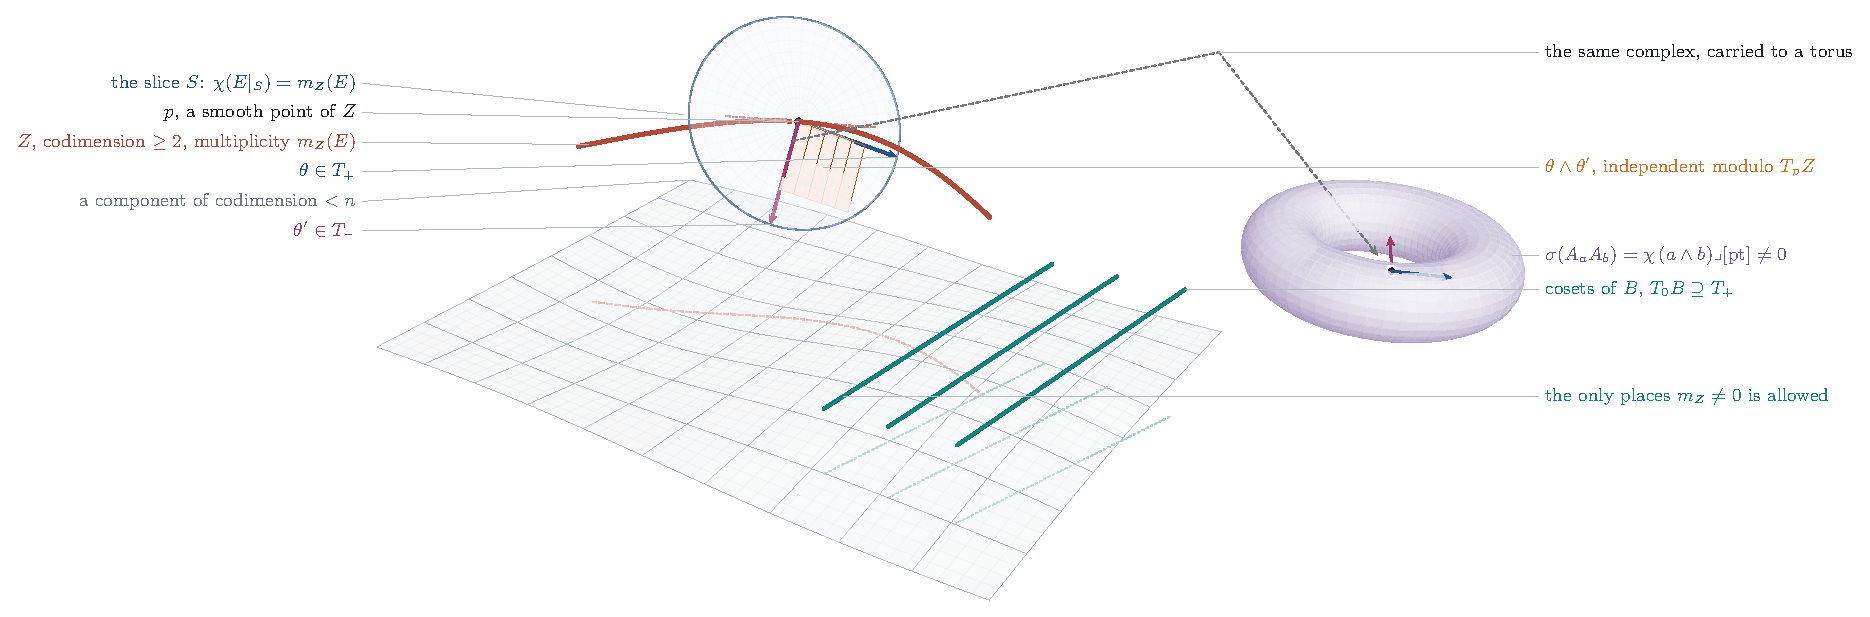
\includegraphics[width=\textwidth]{fig_support}
\caption{The proof of \Cref{thm:p2support}. The grey sheet stands for a
component of the support of codimension less than $n$, which the theorem
forces to exist; the clay curve $Z$ for a component of codimension at least
two. At a smooth point $p$ of $Z$ the directions $\theta\in T_{+}$ and
$\theta'\in T_{-}$ span the slice $S$, transverse to $Z$, on which $E$ restricts
to a complex of finite length with Euler characteristic $m_{Z}(E)$; the amber
parallelogram is the bivector $\theta\wedge\theta'$, independent modulo
$T_{p}Z$. Carried to a torus of the same dimension, the product of the two
jet classes is seen by the semiregularity map as $m_{Z}(E)$ times the class of
a point contracted with the bivector, which is not zero, so $m_{Z}(E)=0$ or
the bivector degenerates. The teal lines are cosets of an abelian subvariety
$B$ tangent to $T_{+}$, the only components of codimension at least two on
which a nonzero multiplicity survives. The scene is schematic in the
dimensions and exact in the incidences.}
\label{fig:support}
\end{figure}

\begin{remark}[What is left of the search]\label{rem:p2search}
Put together, \Cref{thm:p2forces}, \Cref{cor:hhfactor},
\Cref{thm:p2numerical} and \Cref{thm:p2support} describe an object meeting
the criterion at a general member as follows. It has rank zero and first Chern
class zero. Its support has a component of codimension less than $n$,
although its Chern character begins in codimension $n$; at $n=2$ that
component is a divisor or the whole of $A$. Along every component of its
support of codimension at least two its cohomology modules have alternating
length zero, so it has at least two of them there, glued as in the cone of
item (XL). It extends along all $2n^{2}$ $K$-linear deformations of $A$, its
endomorphisms have trace zero, and its Hochschild action factors through a
ring of dimension $2^{2n+1}-1$. The central part of $\Ext^{2}(E,E)$, the image
of $HH^{2}(A)$, has dimension exactly $2n(2n-1)$, and if $\Ext^{2}(E,E)$ is no
larger than its central part, the criterion holds.

The Weil class, which lives in codimension $n$, therefore has to come from the
part of the Chern character that the leading multiplicities do not see: from
twists that cancel in rank but not in higher degree. At $n=2$ the model is a
pair $\cO_{D}$ and $\cO_{D}(W)$ on a divisor $D$, with $W$ a divisor on $D$,
whose difference has Chern character $-i_{*}[W]$ plus terms of higher degree
and has multiplicity zero along $D$. That is a very specific shape, and none
of the objects in the literature or in this paper has it. We record it as the
form the search now takes, and not as a claim that such an object exists.
\end{remark}

\subsubsection*{What the dimension forces on the object}

The numerical criterion of \Cref{thm:p2numerical} fixes one number,
$\dim\Ext^{2}(E,E)$. Together with Serre duality, the lower bounds of
\Cref{cor:hhfactor} in the other degrees and the Hodge--Riemann relations for
the Weil class, it fixes a good deal more: the object that carries the class
can be taken indecomposable, and in the first open case it has more than one
endomorphism. This is where a search has to look.

\begin{theorem}[The shape of an object meeting the criterion]
\label{thm:p2endo}
Let $A$, $\omega$ and $E$ be as in \Cref{thm:p2numerical}, so that
$\ch(E)=N\omega$ with $N\ne0$ and no other component, and suppose that
$\dim\Ext^{2}(E,E)=2n(2n-1)$. Write $e_{k}=\dim\Ext^{k}(E,E)$.
\begin{enumerate}[label=\textup{(\roman*)},leftmargin=2.6em,itemsep=2pt]
\item $\chi(E,E)=\sum_{k}(-1)^{k}e_{k}=(-1)^{n}N^{2}\int_{A}\omega^{2}$, and
  this number is positive.
\item $E\cong E_{0}\oplus E'$ with $E_{0}$ indecomposable,
  $\ch(E_{0})=\ch(E)$, $\dim\Ext^{2}(E_{0},E_{0})=2n(2n-1)$, $\ch(E')=0$ and
  $\Ext^{2}(E_{0},E')=\Ext^{2}(E',E_{0})=\Ext^{2}(E',E')=0$. So $E_{0}$ meets
  the criterion as well.
\item If $E$ is indecomposable, then $\End(E)=\CC\cdot\id\oplus J$ with $J$
  the nilpotent radical, every $f\in J$ annihilates $\Ext^{2}(E,E)$ and
  $\Ext^{2n-2}(E,E)$ under the Yoneda product, and
  $\operatorname{ev}_{E}(\bigwedge^{2n}P)=\operatorname{ev}_{E}(\bigwedge^{2n}Q)$
  is a single line in $\Ext^{2n}(E,E)$. If moreover $e_{1}=4n$, then $J$
  annihilates $\Ext^{1}(E,E)$ as well.
\item If $n=2$ or $n=3$, then
  \[
    \dim\End(E)\;\ge\;2+\tfrac12\,\chi(E,E)\;>\;2,
  \]
  so $E$ has at least three linearly independent endomorphisms, and at
  $n=3$ also $e_{1}\le e_{0}+9$. In particular no simple object meets the
  criterion: no stable sheaf, no complex with $\End=\CC$, and no image of one
  under an autoequivalence of $D^{b}(A)$; and an indecomposable object that
  meets it has a nonzero nilpotent endomorphism. The smallest profiles
  $(e_{0},\dots,e_{2n})$ that the constraints allow are $(3,8,12,8,3)$ at
  $n=2$, with $\chi=2$, and $(3,12,30,40,30,12,3)$ and $(3,12,30,41,30,12,3)$
  at $n=3$, with $\chi=2$ and $\chi=1$.
\end{enumerate}
Parts (i) and (ii), and part (iv) at $n=2$, use the compatibility
$\sigma_{E}\circ\operatorname{ev}_{E}=(\,\cdot\,)\lrcorner\ch(E)$ of
\Cref{setup:hh} in degree two only, as \Cref{thm:p2numerical} does. Part
(iii), and part (iv) at $n=3$, use it in the further degrees in which
\Cref{cor:hhfactor}(iii) grants it: $2n-2$ and $2n$ for (iii), and three for
(iv).
\end{theorem}

\begin{proof}
(i) The Todd class of $A$ is trivial, so the Riemann--Roch theorem gives
$\chi(E,E)=\int_{A}\ch(E)^{\vee}\ch(E)$, and $\ch(E)^{\vee}=(-1)^{n}N\omega$
since $\omega$ has degree $2n$. The polarisation pairs $V_{+}$ only with
$V_{-}$ (\Cref{fig:tangent}), so its class $\theta$ lies in
$V_{+}\otimes V_{-}$ and $\theta\wedge\alpha_{\pm}=0$, because $\alpha_{\pm}$
spans the top exterior power of $V_{\pm}$. So $\omega$ is a nonzero rational
primitive class of type $(n,n)$ in the middle degree, and the Hodge--Riemann
relations give $(-1)^{n(2n-1)}\int_{A}\omega^{2}>0$, where
$(-1)^{n(2n-1)}=(-1)^{n}$. Item (L) of \Cref{sec:verification} checks the
primitivity and the sign of the intersection form on the whole rational Weil
plane in the coordinate model, for $n=2,3$ and several discriminants.

(ii) The category $D^{b}(A)$ has finite dimensional morphism spaces and split
idempotents, so $E=\bigoplus_{i}E_{i}$ with each $E_{i}$ indecomposable. The
evaluation map and the semiregularity map are compatible with direct sums,
and by \Cref{thm:p2numerical}(i) the kernel of $\operatorname{ev}_{E}$ in
degree two is $P\wedge Q$; so $\operatorname{ev}_{E_{i}}(P\wedge Q)=0$ and,
composing with $\sigma_{E_{i}}$, $(P\wedge Q)\lrcorner\ch(E_{i})=0$ for every
$i$. We claim that the only classes of Hodge type killed by $P\wedge Q$ are
those of $\CC\alpha_{+}\oplus\CC\alpha_{-}$. Write
$H^{*}(A,\CC)=\bigwedge^{*}(A_{+}\oplus B_{+}\oplus A_{-}\oplus B_{-})$ with
$A_{\pm}=V_{\pm}^{1,0}$ and $B_{\pm}=V_{\pm}^{0,1}$, and grade it by the four
degrees $(i,j,k,l)$. As in \Cref{setup:hh}, $P$ acts by wedging with $B_{+}$
and contracting $A_{-}$, and $Q$ by wedging with $B_{-}$ and contracting
$A_{+}$, so $P\wedge Q$ is spanned by four kinds of operators, each of which
shifts the four degrees by a fixed amount: wedging with $b_{+}\wedge b_{-}$
kills a component of degree $(i,j,k,l)$ for all choices exactly when $j=n$ or
$l=n$; wedging with $b_{+}$ after contracting $a_{+}$, exactly when $i=0$ or
$j=n$; contracting $a_{-}$ and wedging with $b_{-}$, exactly when $k=0$ or
$l=n$; and contracting $a_{-}$ and $a_{+}$, exactly when $i=0$ or $k=0$. Each
of these is a statement about a tensor product of maps that are injective
unless the degree in question is extreme. A class of type $(p,p)$ has
$i+k=j+l=p$ in every component. If $j=n$, then $l=n$ would force $i=k=n$,
against the fourth condition, so $k=0$, hence $i=n+l$, so $i=n$, $l=0$: the
component lies in $\bigwedge^{n}A_{+}\otimes\bigwedge^{n}B_{+}=\CC\alpha_{+}$.
If $j<n$, then $l=n$ and $i=0$, hence $k=n$ and $j=0$: the component lies in
$\CC\alpha_{-}$. This proves the claim, which item (L) also checks in every
degree for $n=2,3$. Since $\ch(E_{i})$ is rational, it lies on the rational
Weil plane, and when it is nonzero \Cref{cor:hhfactor}(i) gives
$\dim\Ext^{2}(E_{i},E_{i})\ge2n(2n-1)$, a nonzero rational Weil class having
both coefficients $a$ and $b$ nonzero. As
$\Ext^{2}(E,E)=\bigoplus_{i,j}\Ext^{2}(E_{i},E_{j})$ has dimension
$2n(2n-1)$ and $\sum_{i}\ch(E_{i})=N\omega\ne0$, exactly one summand $E_{0}$
has nonzero Chern character and every other block of $\Ext^{2}$ vanishes.

(iii) An indecomposable object of a category with finite dimensional
morphism spaces and split idempotents has a local endomorphism ring, so
$\End(E)=\CC\cdot\id\oplus J$ with $J$ nilpotent. By
\Cref{thm:p2numerical}(i), $\operatorname{ev}_{E}$ maps
$\bigwedge^{2}P\oplus\bigwedge^{2}Q$ isomorphically onto $\Ext^{2}(E,E)$.
By Serre duality $e_{2n-2}=e_{2}$, and contraction with $\omega$ is injective
on $\bigwedge^{2n-2}P\oplus\bigwedge^{2n-2}Q$ (item (L)), so, with the
compatibility in degree $2n-2$, $\operatorname{ev}_{E}$ maps that space
isomorphically onto $\Ext^{2n-2}(E,E)$. In degree $2n$ the semiregularity map is the trace, since
$H^{q+2n}(\Omega^{q}_{A})=0$ for $q>0$, so
$\operatorname{tr}\operatorname{ev}_{E}(\xi)$ is the $H^{0,2n}$ component of
$\xi\lrcorner\ch(E)$; for the generators $\pi_{P}$, $\pi_{Q}$ of
$\bigwedge^{2n}P$ and $\bigwedge^{2n}Q$ it is $Nc_{P}$ and $Nc_{Q}$ with
$c_{P}c_{Q}\ne0$ (item (L)). For $f\in\End(E)$ and
$x\in\bigwedge^{2}P\oplus\bigwedge^{2}Q$ write
$f\cdot\operatorname{ev}_{E}(x)=\operatorname{ev}_{E}(\varphi_{f}(x))$; then
$f\mapsto\varphi_{f}$ is a homomorphism of algebras. Let $x\in\bigwedge^{2}P$
and $y\in\bigwedge^{2n-2}P$, and write $x\wedge y=\beta(x,y)\pi_{P}$. Since
$\operatorname{ev}_{E}$ is a ring map that kills the ideal generated by
$P\wedge Q$,
\[
  \beta(x,y)\operatorname{tr}\bigl(f\operatorname{ev}_{E}(\pi_{P})\bigr)
  =\operatorname{tr}\bigl(f\operatorname{ev}_{E}(x)\operatorname{ev}_{E}(y)\bigr)
  =\operatorname{tr}\operatorname{ev}_{E}\bigl(\varphi_{f}(x)\wedge y\bigr)
  =Nc_{P}\,\beta\bigl(\varphi_{f}(x)_{P},y\bigr),
\]
and the pairing $\beta$ is perfect, so $\varphi_{f}(x)_{P}=\mu_{f}x$ with
$\mu_{f}=\operatorname{tr}(f\operatorname{ev}_{E}(\pi_{P}))/Nc_{P}$. The same
computation with $y\in\bigwedge^{2n-2}Q$, where $x\wedge y=0$ in the quotient,
gives $\varphi_{f}(x)_{Q}=0$. So $f$ acts on
$\operatorname{ev}_{E}(\bigwedge^{2}P)$ by a scalar $\mu_{f}$, and in the same
way on $\operatorname{ev}_{E}(\bigwedge^{2}Q)$ by a scalar $\nu_{f}$; $\mu$ and
$\nu$ are characters of $\End(E)$ and vanish on $J$. So $J$ kills
$\Ext^{2}(E,E)$, on both sides because $\operatorname{ev}_{E}$ lands in the
graded centre, and the same argument with the roles of the two degrees
exchanged shows that it kills $\Ext^{2n-2}(E,E)$. In particular
$\operatorname{tr}(f\operatorname{ev}_{E}(\pi_{P}))=\mu_{f}Nc_{P}=0$ for
$f\in J$, so $\operatorname{ev}_{E}(\pi_{P})$ and, likewise,
$\operatorname{ev}_{E}(\pi_{Q})$ lie in the annihilator of $J$ under the
perfect pairing of $\End(E)$ with $\Ext^{2n}(E,E)$. That annihilator is a
line, $J$ having codimension one, and both elements are nonzero, their traces
being $Nc_{P}$ and $Nc_{Q}$; so they span the same line. Finally, if
$e_{1}=4n$ then $\Ext^{1}(E,E)=\operatorname{ev}_{E}(HH^{1})$, because
$\operatorname{ev}_{E}$ is injective on $HH^{1}$, as shown in (iv). For
$f\in J$ and $h\in HH^{1}$ write $f\operatorname{ev}_{E}(h)=
\operatorname{ev}_{E}(h')$; then
$\operatorname{ev}_{E}(h'\wedge h'')=f\operatorname{ev}_{E}(h\wedge h'')=0$ for
every $h''\in HH^{1}$, so $h'\wedge HH^{1}\subseteq P\wedge Q$, which forces
$h'=0$ since $\dim P=\dim Q\ge2$.

(iv) By Serre duality $e_{k}=e_{2n-k}$. The map $\operatorname{ev}_{E}$ is
injective on $HH^{1}$ using degree two alone: if $\operatorname{ev}_{E}(h)=0$
then $\operatorname{ev}_{E}(h\wedge h')=0$ for every $h'$, so
$h\wedge HH^{1}\subseteq\Ann_{HH^{2}}(\omega)=P\wedge Q$, and $h=0$ as in
(iii). So $e_{1}\ge4n$, and \Cref{cor:hhfactor}(iii) gives
$e_{3}\ge2\binom{6}{3}=40$ at $n=3$. At $n=2$ the Euler
characteristic is $2e_{0}-2e_{1}+12$, and at $n=3$ it is
$2e_{0}-2e_{1}+60-e_{3}$. So $2e_{0}=\chi+2e_{1}-12\ge\chi+4$ at $n=2$, and
$2e_{0}=\chi+2e_{1}+e_{3}-60\ge\chi+4$ at $n=3$, where also
$e_{1}=e_{0}+30-\frac12(\chi+e_{3})\le e_{0}+9$. With (i) this gives the
bound. An autoequivalence preserves $\End$, and a stable sheaf is simple.
An indecomposable object with $\dim\End\ge3$ has $J\ne0$. The smallest
profiles are those with $e_{0}=3$, which item (L) lists by exhaustive search
over the admissible values, and Section 31 of the Lean certificate checks the
inequality $e_{0}\ge3$ for all natural numbers.
\end{proof}

\begin{remark}[What the shape does to the search]\label{rem:p2endo}
\Cref{thm:p2endo} is a necessary condition and nothing more; it does not say
that an object meeting the criterion exists. What it does is remove from the
search every object that anyone would construct first. Line bundles,
semi-homogeneous bundles, skyscraper sheaves, stable sheaves and their
Fourier--Mukai transforms are simple, and direct sums of them are excluded by
(ii) together with \Cref{thm:nosum}. At $n=3$, the first open case, what
remains is an indecomposable object with a local endomorphism algebra of
dimension at least three whose radical kills $\Ext^{2}$ and $\Ext^{4}$ and
pairs to zero with the line $\operatorname{ev}_{E}(\bigwedge^{6}P)$,
granting the compatibility of \Cref{cor:hhfactor}(iii); the smallest
conceivable one has $\Hom(E,E)$ of dimension three, $\Ext^{1}(E,E)$
equal to the image of $HH^{1}(A)$, of dimension twelve and killed by the
radical, and $\Ext^{3}(E,E)$ of dimension forty or forty-one. Iterated
self-extensions and thickenings are the natural objects with nilpotent
endomorphisms; an extension of a simple object $F$ by itself has
$\ch=2\ch(F)$, so $F$ would have to carry the class already, and the question
returns one level down. Nothing in this paper produces an object of the
required shape, and the remark is recorded as the form the search now takes.
For $n\ge4$ the same count only asks for an excess in some even degree other
than $2$ and $2n-2$ (item (L)), and the bound on $\End$ disappears.
\end{remark}

\subsubsection*{The pure form of the criterion is never met}

So far $\ch(E)=N\omega$ exactly. If $\sigma_{E}$ were injective, $E$ would
extend along every $K$-linear deformation of $A$ (\Cref{thm:p2forces}(ii)).
These reach non-algebraic tori, on which the Weil class is Hodge and the Chern
class of nothing. That settles the pure form of the criterion, negatively, in
every dimension.

\begin{setupenv}[Weil tori]\label{setup:weiltori}
Let $A$ be an abelian $2n$-fold of $(K,-1,n)$-Weil type, $V=H^{1}(A,\QQ)$ with
its action of $K$, and $V\otimes\CC=V_{+}\oplus V_{-}$ the two eigenspaces,
each of dimension $2n$. For complementary $n$-dimensional subspaces
$X,Y\subset V_{+}$ the subspace $X\oplus\bbar{Y}$ of $V\otimes\CC$ is the
space of holomorphic $1$-forms of a complex structure on the real torus
underlying $A$; call the resulting complex torus $T_{X,Y}$. On $T_{X,Y}$ the
field $K$ acts with signature $(n,n)$, so $T_{X,Y}$ is a Weil torus in the
sense of \cite{Voi02b}, and every complex structure on that real torus
commuting with $K$ and of signature $(n,n)$ arises in this way. The pairs
$(X,Y)$ form a connected complex manifold $S$ of dimension $2n^{2}$,
containing the point of $A$; the polarised Weil family is the submanifold of
dimension $n^{2}$ on which the polarisation of $A$ is of type $(1,1)$, and the
tangent space of $S$ is the space $\Hom_{K}(H^{1,0},H^{0,1})$ of $K$-linear
first order deformations in \Cref{thm:p2forces}(i). Since
$\alpha_{+}$ spans $\bigwedge^{2n}V_{+}=\bigwedge^{n}X\otimes\bigwedge^{n}Y$
and $X$ is holomorphic while $Y$ is antiholomorphic, the Weil classes are of
type $(n,n)$ on every $T_{X,Y}$. We say that a property holds for a very
general member of $S$ if it holds outside a countable union of proper
analytic subsets.
\end{setupenv}

\begin{lemma}[The Hodge classes of a very general Weil torus]
\label{lem:weiltorushodge}
For a very general member $T$ of $S$, $\Hdg^{k}(T)=0$ for
$1\le k\le2n-1$, $k\ne n$, and $\Hdg^{n}(T)$ is the rational Weil plane.
\end{lemma}

\begin{proof}
A rational class that is of Hodge type at a very general member is of Hodge
type on all of $S$, because its Hodge locus is analytic and $S$ is connected.
Let $G=\Res_{K/\QQ}\mathrm{GL}_{2n}$ be the group of $K$-linear automorphisms
of $V$. Its real points act transitively on $S$, since
$\mathrm{GL}(V_{+})$ acts transitively on pairs of complementary subspaces.
The Mumford--Tate group $M$ of a very general member lies in $G$, since $K$
acts by endomorphisms of every member, and it contains the Mumford--Tate group
of every member, whose Hodge classes include those of the very general one.
So the real Lie algebra of $M$ contains the complex structure $J_{s}$ of every
member, the derivative of its Hodge cocharacter, and therefore contains the $\mathrm{Ad}\,G(\RR)$-span of one $J_{s}$, which is an ideal of
$\mathfrak{g}_{\RR}=\mathfrak{gl}_{2n}(\CC)$ containing a non-central
element, $J_{s}$ acting on $V_{+}$ by $i$ on $X$ and $-i$ on $Y$; hence it
contains $\mathfrak{sl}_{2n}(\CC)$, and $M$ contains
$G^{\mathrm{der}}=\Res_{K/\QQ}\mathrm{SL}_{2n}$. Over $\CC$ this is
$\mathrm{SL}(V_{+})\times\mathrm{SL}(V_{-})$ acting on
$\bigwedge^{*}(V_{+}\oplus V_{-})=\bigwedge^{*}V_{+}\otimes\bigwedge^{*}V_{-}$,
whose invariants are spanned by $1$, $\alpha_{+}$, $\alpha_{-}$ and
$\alpha_{+}\alpha_{-}$. Hodge classes are invariant under $M$, which gives
the statement. Item (LI) of \Cref{sec:verification} confirms it for $n=2$
and $n=3$ by exhibiting explicit members at which no other rational class of
those degrees is of Hodge type.
\end{proof}

\begin{lemma}[A very general Weil torus has no subvarieties]
\label{lem:weiltorussubsets}
A very general member $T$ of $S$ has no analytic subsets other than finite
sets and $T$ itself.
\end{lemma}

\begin{proof}
Let $Z\subset T$ be an irreducible analytic subset of codimension $c$ with
$0<c<2n$. For every K\"ahler class $\kappa$ the class $[Z]$ satisfies
$\int_{T}[Z]\,\kappa^{2n-c}=\int_{Z}\kappa^{2n-c}>0$, so $[Z]$ is a nonzero
Hodge class of degree $2c$. By \Cref{lem:weiltorushodge} this forces $c=n$ and
$[Z]$ into the Weil plane. Take for $\kappa_{0}$ the class of a positive
definite hermitian form that is block diagonal for the splitting
$H^{1,0}=X\oplus\bbar{Y}$. Its blocks lie in $X\otimes\bbar{X}$ and
$\bbar{Y}\otimes Y$, both inside $V_{+}\otimes V_{-}$, so every power of
$\kappa_{0}$ has a factor from $V_{+}$ and a factor from $V_{-}$ in each term,
and $\alpha_{\pm}\wedge\kappa_{0}^{n}=0$ because $\alpha_{\pm}$ spans the top
exterior power of $V_{\pm}$ (item (LI)). So
$\int_{T}[Z]\,\kappa_{0}^{n}=0$, which is impossible.
\end{proof}

\begin{proposition}[Coherent sheaves on a very general Weil torus]
\label{prop:weiltorussheaves}
Let $n\ge2$ and let $T$ be a very general member of $S$. Every coherent
analytic sheaf $F$ on $T$ has $\ch_{k}(F)=0$ in $H^{2k}(T,\QQ)$ for
$1\le k\le2n-1$. For $n=2$ this is Voisin's theorem that every coherent sheaf
on a general Weil torus of dimension four has $c_{2}(F)=0$
\cite[Theorem~10]{Voi02b}, whose proof we follow.
\end{proposition}

\begin{proof}
Chern classes of coherent sheaves on $T$ exist in rational Deligne
cohomology, extend those of bundles and are additive \cite{Gri10}, so they
are Hodge classes. By \Cref{lem:weiltorussubsets} the torsion of $F$, the locus where the
torsion-free quotient is not locally free, and the cokernel of the map from
that quotient to its reflexive hull are all supported on finite sets, and a
sheaf supported on a finite set has Chern character in the top degree only. So
it suffices to treat a reflexive sheaf $G$. Every coherent sheaf on $T$ has
$c_{1}=0$, since $\Hdg^{1}(T)=0$ (\Cref{lem:weiltorushodge}); so every
torsion-free sheaf has slope zero for every K\"ahler class, and a torsion-free
sheaf is stable for one K\"ahler class exactly when it has no saturated
subsheaf of intermediate rank, which does not depend on the class. A
Jordan--H\"older filtration of $G$ therefore has stable torsion-free factors
$Q_{j}$, stable for every K\"ahler class, and $\ch(G)=\sum_{j}\ch(Q_{j})$.
By the theorem of Bando and Siu \cite{BS94} the stable reflexive sheaf
$Q_{j}^{**}$ carries an admissible Hermite--Einstein metric for every K\"ahler
class $\kappa$ and satisfies
$\int_{T}\bigl(2rc_{2}-(r-1)c_{1}^{2}\bigr)(Q_{j}^{**})\,\kappa^{2n-2}\ge0$,
with equality exactly when $Q_{j}^{**}$ is a projectively flat vector bundle.
Here $c_{1}=0$ and $c_{2}(Q_{j}^{**})\in\Hdg^{2}(T)$. For $n\ge3$ that group is
zero; for $n=2$ it is the Weil plane, and then
$\int_{T}c_{2}(Q_{j}^{**})\,\kappa_{0}^{2}=0$ for the class $\kappa_{0}$ of
the proof of \Cref{lem:weiltorussubsets}. In either case equality holds for
some $\kappa$, so $Q_{j}^{**}$ is a projectively flat bundle with $c_{1}=0$,
hence flat, and its rational Chern classes of positive degree vanish.
$Q_{j}$ and $Q_{j}^{**}$ differ on a finite set, so $\ch_{k}(Q_{j})=0$ for
$1\le k\le2n-1$, and the same holds for $G$ and for $F$.
\end{proof}

\begin{theorem}[The pure form of the criterion is never met]
\label{thm:p2false}
Let $n\ge2$, let $A$ be an abelian $2n$-fold of $(K,-1,n)$-Weil type, $\omega$
a nonzero rational Weil class, and $E$ a perfect complex on $A$ with
$\ch(E)=N\omega$, $N\ne0$, and no other component. Then $\sigma_{E}$ is not
injective. In particular $\dim\Ext^{2}(E,E)>2n(2n-1)$, the hypotheses of
\Cref{thm:semiregclosure} and \Cref{thm:p2numerical}(iii) are satisfied by no
object at any member of any Weil family of an imaginary quadratic field, and
the propagation statement \textup{(P2)} of \Cref{rem:tworemain}, in the form
stated there, is false.
\end{theorem}

\begin{proof}
Suppose $\sigma_{E}$ injective. Since $A$ is projective, $E$ is isomorphic to
a bounded complex $E^{\bullet}$ of holomorphic vector bundles. The class
$N\omega$ is of Hodge type on every member of $S$ (\Cref{setup:weiltori}), so
by the theorem of Buchweitz and Flenner in Pridham's form (\Cref{thm:BF},
\cite{BF03,Pri24}), every obstruction to extending $E$ along an
Artinian deformation of $A$ inside $S$ vanishes, exactly as in the proof of
\Cref{thm:semiregclosure}. The deformations of the complex structure inside
$S$ together with those of the holomorphic structures and differentials of
$E^{\bullet}$ are governed by a differential graded Lie algebra of Dolbeault
type with finite dimensional cohomology, and Kuranishi's method
\cite{Kur65}, in the form of \cite[Sections~2--3]{GM88}, gives an analytic
germ $(M,m_{0})$ with a morphism $\pi\colon(M,m_{0})\to(S,s_{0})$ and a
complex of holomorphic vector bundles on the pulled back family of tori
deforming $E^{\bullet}$, whose completion is a hull of the formal deformation
functor. The vanishing of the obstructions says that $\pi$ is formally
smooth, hence smooth, so its image contains a neighbourhood $U$ of $s_{0}$.
Thus every member $T_{s}$ with $s\in U$ carries a bounded complex of
holomorphic vector bundles $E_{s}^{\bullet}$ whose Chern character is the
parallel transport of $N\omega$. Choose $s\in U$ very general. By
\Cref{prop:weiltorussheaves},
$\ch_{n}(E_{s})=\sum_{i}(-1)^{i}\ch_{n}(E_{s}^{i})=0$, while it is the
transport of $N\omega$, which is not zero. This contradiction proves that
$\sigma_{E}$ is not injective. The argument uses only that $\ch(E)$ is of
Hodge type on every member of $S$, so it applies verbatim when $\ch(E)-N\omega$
has components in degrees $0$ and $4n$ as well. The remaining statements
follow, since $\dim\Ext^{2}(E,E)\ge2n(2n-1)$ by \Cref{cor:hhfactor}(i),
and equality forces $\sigma_{E}$ to be injective by
\Cref{thm:p2numerical}(i).
\end{proof}

\begin{remark}[What survives, and the corrected statement]\label{rem:p2prime}
\Cref{thm:p2false} turns \Cref{thm:p2forces}(ii) from a constraint into a
contradiction: an object that extends along every $K$-linear deformation of
$A$ lands on non-algebraic tori, where the Weil class is Hodge and is the
Chern class of nothing. The results of this part that describe the object,
\Cref{thm:p2forces}, \Cref{cor:hhfactor}(ii)--(iii), \Cref{thm:p2numerical},
\Cref{thm:p2support}, \Cref{thm:nosum} and \Cref{thm:p2endo}, remain true as
implications, and they are vacuous: no object satisfies their hypotheses. They
are kept as the record of what the pure form asked for.

The obstruction does not reach a Chern character with a component that is
Hodge on the polarised family and not beyond it, unless a twist removes that
component. Call
\textup{(P2$'$)} the statement that at one base point of each Weil family
some perfect complex $E$ with
\[
  \ch(E)=N\omega_{1}+\sum_{k}c_{k}\,\theta^{k},\qquad N\ne0,\ c_{k}\in\QQ,
\]
$\theta$ the polarisation, has injective semiregularity map. The proof of
\Cref{thm:semiregclosure} applies to it word for word, with the deformation
taken over the polarised family, along which $\ch(E)$ stays of Hodge type:
at a member $A_{s}$ it produces $\ch_{n}(E_{s})=N\omega_{1}+c_{n}\theta^{n}$
algebraic, and $\theta^{n}$ is algebraic, so $\omega_{1}$ is. The form above
is already the most general one allowed by the subring generated by $\theta$
and the Weil classes: a Weil class is primitive, so $\theta\omega_{1}=0$ and
that subring is spanned by the powers of $\theta$ and the Weil plane.
\Cref{thm:p2false} excludes directly a Chern character that remains of Hodge
type on all of $S$, which by \Cref{lem:weiltorushodge} is a multiple of the
Weil class plus terms in degrees $0$ and $4n$, and after a line bundle twist
the characters $c\,e^{t\theta}+N\omega_{1}+c'\theta^{2n}$ with $t\theta$
integral (\Cref{thm:p2primenumber}(v)). For every other corrected character
with some $c_{k}\ne0$, $1\le k\le2n-1$, the component of the Hodge locus of
$\ch(E)$ through $A$ is the polarised family itself, whose members are
abelian varieties, so nothing forces $E$ onto non-algebraic tori and the
argument cannot be run on $E$ (\Cref{prop:p2primelocus}); the one exception is
a ratio at $n=2$ at which the locus is five-dimensional
(\Cref{rem:p2primeexceptional}). The semiregular objects in Markman's
proofs for abelian fourfolds and for the sixfolds of trivial discriminant
\cite{Mar25a,Mar25b} are not of the pure form either: their Chern characters
are not multiples of a Weil class, and they are deformed only along families
on which those characters stay of Hodge type. We have not checked that they
have exactly the form above, and nothing below depends on it. From here on, in
\Cref{cor:fourremain}, \Cref{thm:closure} and the frontier, \textup{(P2)} is
read in this corrected form. The annihilator computations above depend on
$\ch(E)$ being a pure Weil class; they are redone for a Chern character with
components in every even degree at the end of this subsection
(\Cref{thm:p2primenumber}, \Cref{prop:p2primeprofile},
\Cref{prop:p2primelocus}).

The same obstruction does not reach the Mumford target of
\Cref{ssec:mumfordrigid}. The exceptional classes there are rigid: their Hodge
locus among all complex tori is the Mumford curve (\Cref{thm:mumfordrigid},
\Cref{prop:notwistor}), so a semiregular complex with Chern character
$N\omega$ on the square of a Mumford fourfold would only have to deform along
the curve, whose members are all algebraic.
\end{remark}

\begin{remark}[The two finite statements, and what each of them is]
\label{rem:tworemain}
After \Cref{thm:degreebound} and \Cref{thm:semiregclosure} the Hodge
conjecture for abelian varieties of Weil type follows from either of the
following, each of which is a statement about explicit finite data and neither
of which mentions a general point. The first is settled by
\Cref{thm:p1equivalent}, and we record it because it is the form in which the
question first presents itself. The second is settled by \Cref{thm:p2false}
in the form stated here, and remains open only in the corrected form of
\Cref{rem:p2prime}.

\begin{enumerate}[label=\textup{(P\arabic*)},leftmargin=*]
\item \emph{A bound.} At every point of the orbit $G(\QQ)\cdot s_{0}$ the
  class $\omega$ is represented by a cycle whose Hilbert data comes from one
  finite set. This one is settled, and negatively, in the sense that matters:
  \Cref{thm:p1forces} shows that the transport of the base cycle does not
  satisfy it, for any cycle whose components have finite stabiliser, and
  \Cref{thm:p1equivalent} shows that read on an arbitrary representative it is
  equivalent to $\mathbf{W}(K,n,\delta)$ itself. It is therefore a
  reformulation of the conjecture for the family, and we record it as such
  rather than as a criterion.
\item \emph{A rank.} The semiregularity map of a perfect complex with the
  Chern character of \Cref{prop:ktheory} at one base point is injective.
  In this form the statement is false (\Cref{thm:p2false}), and it survives
  only in the corrected form of \Cref{rem:p2prime}, where the Chern
  character may carry powers of the polarisation; what follows records what
  the first form asked for. Its
  source is $\Ext^{2}(E,E)$ for a single object, and its target has dimension
  $\sum_{q}h^{q,q+2}(A_{0})=\binom{4n}{2n-2}$, computed in
  \Cref{prop:target} and verified in item (V) of
  \Cref{sec:verification}. So the target is large, which is the direction that
  helps; what is not known to us is the rank of the map. What is known is
  what full rank would force (\Cref{thm:p2forces}): the evaluation map of
  Hochschild cohomology must vanish on the $4n^{2}$-dimensional annihilator of
  the Weil class, so $E$ must be killed by the mixed block of $H^{0,2}$, must
  extend along every $K$-linear deformation, must have all products of
  transverse translation classes zero, and must have no endomorphism of
  nonzero trace; and at a base point with no abelian subvariety tangent to an
  eigenspace it can be a locally free sheaf on no smooth germ of its support
  of codimension at least two (\Cref{cor:p2shape}). The representative that
  the construction supplies, a virtual sum of line bundles, fails at the first
  of these (\Cref{prop:concentrated}), and any representative that is a
  sheaf fails at the last. \Cref{thm:hhsplitting} adds the shape of that
  annihilator, the mixed part of a splitting $HH^{1}=P\oplus Q$ into the
  annihilators of the two conjugate pieces of the class, and
  \Cref{cor:hhfactor} the consequence: the whole Hochschild action of $E$
  factors through a ring of dimension $2^{2n+1}-1$ inside one of dimension
  $2^{4n}$, while $\dim\Ext^{2}(E,E)\ge2n(2n-1)$ for every representative,
  semiregular or not. \Cref{thm:p2numerical} turns the rank into that number:
  equality is enough. And \Cref{thm:p2support} places the support. At every
  member it has a component of codimension less than $n$, so no complex
  carried by a cycle representing $\omega$ can serve, and at a general member
  every component of codimension at least two has multiplicity zero.
  \Cref{thm:p2endo} fixes its shape: an indecomposable summand carries the
  class and meets the criterion alone, and at $n=2$, and at $n=3$ granting
  the compatibility of \Cref{cor:hhfactor}(iii), it has at least three
  independent endomorphisms, so no simple object serves.
\end{enumerate}

Two remarks on what these are not. Neither is the variational Hodge
conjecture: (P1) said nothing about deformations at all, and (P2) is the
infinitesimal statement at one point with the global propagation already
supplied by \Cref{thm:closedlocus}, which is what \Cref{rem:variational} said
was missing. And neither is implied by the results of
\Cref{ssec:everyfamily}: the base points are there, the cycles are there, and
both (P1) and (P2) are questions about those same cycles that the construction
does not answer. We have not settled either, and we do not claim the
conjecture.
\end{remark}

\subsubsection*{The corrected criterion, computed}

The annihilator computations of this subsection depend on $\ch(E)$ being a
pure Weil class, as \Cref{rem:p2prime} notes. We now redo them for a Chern character with components in every
even degree. In degree two the answer is complete and holds for every $n$;
in the other degrees it is a closed formula, proved away from the middle
degree and checked in it. The same computation gives the Hodge locus of the
character, and with it the list of obstructions of this paper that survive
the correction (\Cref{prop:p2primelocus}, \Cref{rem:p2primesurvive}). None
of this constructs an object or decides
whether one exists. It gives, for each shape of Chern character, the number
that $\dim\Ext^{2}(E,E)$ has to reach and the exact kernel that
$\operatorname{ev}_{E}$ must then have, which is the form in which a
candidate can be tested.

\begin{setupenv}[Corrected characters]\label{setup:p2prime}
Let $A$ be an abelian $2n$-fold of $(K,-1,n)$-Weil type, $n\ge2$, with
polarisation $\theta$, and let $\omega=u\alpha_{+}+\bbar u\,\alpha_{-}$ be a
nonzero real class on the Weil line, in the notation of \Cref{thm:p2forces}.
For complex numbers $c_{0},\dots,c_{2n}$ put
\[
  p(\theta)=\sum_{k=0}^{2n}c_{k}\theta^{k},\qquad
  \gamma=\omega+p(\theta),\qquad \mu_{m}=m!\,c_{m},
\]
and let $\rho\in\{0,1,2,3\}$ be the rank of the $(2n-1)\times3$ Hankel matrix
$H=[\mu_{j+i}]$, $0\le j\le2n-2$, $0\le i\le2$.\footnote{$H$ is a
catalecticant of the moment sequence $\mu_{m}=m!\,c_{m}$. A nonzero vector
$(x,\lambda,w)$ in its kernel is a linear recurrence
$x\mu_{j}+\lambda\mu_{j+1}+w\mu_{j+2}=0$ of order at most two, so $\rho\le2$
says that the moments satisfy one, and the shapes of
\Cref{thm:p2primenumber}(ii) are its solutions, read off from the roots of
$wT^{2}+\lambda T+x$.} Write $r(\gamma)$ for the
rank of contraction $HT^{2}(A)\to H^{*}(A,\CC)$, $\xi\mapsto\xi\lrcorner\gamma$.
For $a<n\le b$, in the basis of \Cref{thm:hhsplitting} adapted to an
eigenbasis $e_{j}$ of $V_{+}$ and $f_{j}$ of $V_{-}$ with $e_{j},f_{j}$ of
type $(1,0)$ for $j<n$ and $j\ge n$ respectively, write
$z_{ab}=w(e_{b})w(f_{a})\in V_{+}^{0,1}\otimes V_{-}^{0,1}$,
$v^{1}_{ab}=w(e_{b})c(e_{a})$ and $v^{2}_{ab}=w(f_{a})c(f_{b})$ in
$H^{1}(T_{A})$, and $\pi_{ab}=c(e_{a})c(f_{b})\in T_{+}\otimes T_{-}$, where
$w$ is wedge product with a $(0,1)$ class and $c$ contraction of a $(1,0)$
class.
\end{setupenv}

For a Chern character, $\gamma=N\omega_{1}+\sum_{k}c_{k}\theta^{k}$ with
rational $c_{k}$, and $u$ is determined by $N\omega_{1}$; intrinsically,
$|u|^{2}=(-1)^{n}\tfrac{(2n)!}{2}\int_{A}\omega^{2}\big/\!\int_{A}\theta^{2n}$
in the normalisation of item (LII). The rank $\rho$ does not change when
$\gamma$ is multiplied by $e^{t\theta}$, which acts on the moments by a
binomial transform, and $\omega e^{t\theta}=\omega$ because a Weil class is
primitive; so $\rho$ is an invariant of $\gamma$ up to twist.

\begin{theorem}[The corrected criterion is a number]\label{thm:p2primenumber}
In \Cref{setup:p2prime}:
\begin{enumerate}[label=\textup{(\roman*)},leftmargin=2.6em,itemsep=2pt]
\item For $n\ge3$,
  \[
    \Ann_{HT^{2}}(\gamma)=\bigoplus_{a<n\le b}
    \bigl\{x\,z_{ab}+y_{1}v^{1}_{ab}+y_{2}v^{2}_{ab}+w\,\pi_{ab}\;:\;
      (x,\;i(y_{1}-y_{2}),\;w)\in\ker H\bigr\},
  \]
  so that $\dim\Ann_{HT^{2}}(\gamma)=n^{2}(4-\rho)$ and
  $r(\gamma)=(4+\rho)n^{2}-2n$, whatever $u\ne0$ is.
\item $\rho=3$ for a general $p$. If $\rho=3$, and either $n\ge3$ or $n=2$ and
  $e=0$ in the notation of (iii), then $\Ann_{HT^{2}}(\gamma)$ is exactly
  the tangent space $T_{[A]}\cD_{n,n}$ of the polarised Weil family, spanned
  by the $n^{2}$ vectors $v^{1}_{ab}+v^{2}_{ab}$, inside $H^{1}(T_{A})$, with
  no component in $H^{0,2}$ or in $H^{0}(\bigwedge^{2}T_{A})$; and
  $r(\gamma)=\binom{4n}{2}-n^{2}=7n^{2}-2n$. Moreover $\rho\le2$ exactly when
  $p$ is one of $Ae^{s\theta}+Be^{t\theta}$, $(A+B\theta)e^{t\theta}$,
  $Ae^{t\theta}+B\theta^{2n}$, $A\theta^{2n-1}+B\theta^{2n}$, and $\rho\le1$
  exactly when $p\in\CC e^{t\theta}\cup\CC\theta^{2n}$; the pure case
  $\rho=0$ gives back $r=2n(2n-1)$ of \Cref{cor:hhfactor}(i).
\item For $n=2$, $\dim\Ann_{HT^{2}}(\gamma)=4(4-\rho)+e$ with
  $e=\dim\ker\bigl((HK)^{2}-|u|^{2}\bigr)\le2$ and $K$ the antidiagonal
  matrix with entries $1,-2,1$; so $r(\gamma)\in\{12,16,18,20,22,23,24\}$,
  and $e>0$ exactly when $X(X-I)^{2}=4J^{2}$, where $X=|u|^{2}$ and $I$, $J$
  are the two invariants of the binary quartic
  $\sum_{m}\binom{4}{m}\mu_{m}x^{4-m}y^{m}$.
\item Let $E$ be a perfect complex on $A$ with $\ch(E)=\gamma$ and $N\ne0$.
  Then $\dim\Ext^{2}(E,E)\ge r(\gamma)$ with no hypothesis on $\sigma_{E}$.
  If equality holds, then $\operatorname{ev}_{E}$ is onto with kernel
  $\Ann_{HT^{2}}(\gamma)$ and $\sigma_{E}$ is injective, so that
  \textup{(P2$'$)} holds at that point and, by \Cref{rem:p2prime} and
  \Cref{thm:semiregclosure}, the Hodge conjecture holds for every member of
  the family with full Hodge group. Conversely, if $\sigma_{E}$ is injective
  then $\ker\operatorname{ev}_{E}=\Ann_{HT^{2}}(\gamma)$.
\item If $p\in\CC e^{t\theta}+\CC\theta^{2n}$ with $t\theta$ the class of a line
  bundle $L$, a set of shapes with $\rho\le2$ that contains
  $\CC\theta^{2n}$, then no perfect complex $E$ with $\ch(E)=\gamma$ has
  injective $\sigma_{E}$.
\end{enumerate}
\end{theorem}

\begin{proof}
(i) Let the torus $(\CC^{\times})^{2n}$ act by $e_{j}\mapsto\tau_{j}e_{j}$,
$f_{j}\mapsto\tau_{j}^{-1}f_{j}$. It preserves the Hodge decomposition and
$\theta$, and scales $\alpha_{\pm}$ by $(\prod_{j}\tau_{j})^{\pm1}$;
contraction is equivariant. A weight of $HT^{2}$ has at most two nonzero
coordinates, so for $n\ge3$ two such weights never differ by a nonzero
multiple of $(1,\dots,1)$, and the images of one weight component in the
$\theta$-part and in the two $\alpha$-parts land in distinct weight spaces.
Hence $\Ann(\gamma)=\Ann(p(\theta))\cap\Ann(\alpha_{+})\cap\Ann(\alpha_{-})$,
and the last two meet in $P\wedge Q$ by \Cref{thm:hhsplitting}(ii). The space
$P\wedge Q$ is the sum over $a<n\le b$ of the four-dimensional weight spaces
spanned by $z_{ab},v^{1}_{ab},v^{2}_{ab},\pi_{ab}$, and $\Ann(p(\theta))$ is
torus-stable, so the computation splits pair by pair. Put
$m=e_{b}\wedge f_{a}$ and $\theta'=\theta-t_{a}-t_{b}$, where
$t_{j}=i s_{j}e_{j}\wedge f_{j}$ with $s_{j}=\pm1$ the sign that makes
$\theta=\sum_{j}t_{j}$ positive. Since the $t_{j}$ are even with
$t_{j}^{2}=0$, direct evaluation gives
\[
  z\lrcorner\theta^{k}=m\,\theta'^{k},\quad
  v^{1}\lrcorner\theta^{k}=ik\,m\,\theta'^{k-1},\quad
  v^{2}\lrcorner\theta^{k}=-ik\,m\,\theta'^{k-1},\quad
  \pi\lrcorner\theta^{k}=k(k-1)\,m\,\theta'^{k-2},
\]
so for $\xi=xz+y_{1}v^{1}+y_{2}v^{2}+w\pi$ and $\lambda=i(y_{1}-y_{2})$,
\[
  \xi\lrcorner p(\theta)=m\wedge\sum_{j=0}^{2n-2}\frac{\theta'^{j}}{j!}
  \bigl(x\mu_{j}+\lambda\mu_{j+1}+w\mu_{j+2}\bigr).
\]
The classes $m\wedge\theta'^{j}$, $0\le j\le2n-2$, are nonzero and of distinct
degrees, so $\xi$ kills $p(\theta)$ exactly when $(x,\lambda,w)\in\ker H$.
The map $(x,y_{1},y_{2},w)\mapsto(x,\lambda,w)$ is onto with kernel spanned by
$v^{1}+v^{2}$, which gives $1+(3-\rho)$ dimensions for each of the $n^{2}$
pairs. (ii) The vector $v^{1}_{ab}+v^{2}_{ab}$ is $K$-linear and kills
$\theta$, and these $n^{2}$ vectors span the tangent space of the polarised
family by \Cref{prop:firstorder}; when $\rho=3$ they are all of the
annihilator. If $\rho\le2$, a nonzero $(x,\lambda,w)\in\ker H$ turns the
equations $x\mu_{j}+\lambda\mu_{j+1}+w\mu_{j+2}=0$ into a linear recurrence of
full rank on $\mu_{0},\dots,\mu_{2n}$, whose two-dimensional space of
solutions is spanned by the listed shapes according to the roots of
$wT^{2}+\lambda T+x$; $\rho\le1$ is the intersection of two such spaces.
(iii) At $n=2$ the argument of (i) fails for exactly one pair of weights,
$\epsilon_{2}+\epsilon_{3}$ in $\bigwedge^{2}P$ and $-\epsilon_{0}-\epsilon_{1}$
in $\bigwedge^{2}Q$, whose difference is $(1,1,1,1)$; these give one coupled
block of size eight, whose kernel is isomorphic to $\ker(X-T)$ with $T$
conjugate on its image to $(HK)^{2}$, and the characteristic polynomial of
$HK$ is $y^{3}-Iy-2J$, which is traceless, so $e\le2$. (iv) is the argument of
\Cref{thm:p2numerical}(i)--(ii) with $\Ann_{HT^{2}}(\gamma)$ in place of
$P\wedge Q$: $\sigma_{E}\circ\operatorname{ev}_{E}$ is contraction into
$\gamma$, so $\ker\operatorname{ev}_{E}\subseteq\Ann_{HT^{2}}(\gamma)$. (v) If
$\gamma-\omega$ has components in degrees $0$ and $4n$ only, the proof of
\Cref{thm:p2false} applies verbatim. If $p=c\,e^{t\theta}+c'\theta^{2n}$ with
$t\theta=c_{1}(L)$, then
$\ch(E\otimes L^{-1})=\gamma e^{-t\theta}=c+\omega+c'\theta^{2n}$, because
$\omega\theta=0$ and $\theta^{2n+1}=0$, and
$\sigma_{E\otimes L^{-1}}=e^{-c_{1}(L)}\cdot\sigma_{E}$ is injective exactly
when $\sigma_{E}$ is, so the first case applies to $E\otimes L^{-1}$.
Item (LII) of \Cref{sec:verification} computes the annihilator structure-free,
exactly over $\QQ(i)$, for $n\le10$, and checks every statement above.
\end{proof}

So the number that the corrected criterion asks of one complex is $24$ at
$n=2$, $57$ at $n=3$ and $104$ at $n=4$ for a general shape, against $12$,
$30$ and $56$ for the pure form, and injectivity then forces nothing beyond
first-order extension along the polarised family, which is what the
criterion is for. The larger number is the price of the components
$c_{k}\theta^{k}$, and it is paid in the right place: every direction of
$HT^{2}$ other than the $n^{2}$ directions of the family moves $\gamma$ off
the Hodge classes, so an object meeting the bound has $\operatorname{ev}_{E}$
injective on a complement of $T_{[A]}\cD_{n,n}$.
\Cref{fig:hankel} plots the number against $n$ for the four Hankel ranks.

\begin{figure}[tbp]
\centering
  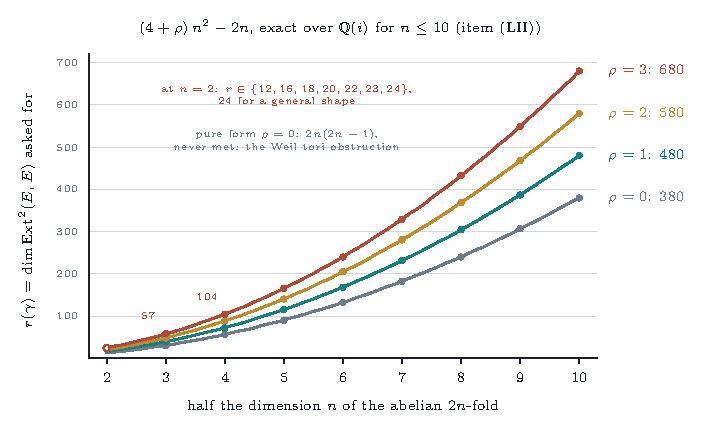
\includegraphics[width=0.86\textwidth]{fig_hankel}
\caption{The dimension $r(\gamma)=(4+\rho)n^{2}-2n$ that
$\Ext^{2}(E,E)$ must have for a complex with Chern character
$\gamma=N\omega_{1}+\sum_{k}c_{k}\theta^{k}$ to meet the corrected criterion,
for the four Hankel ranks $\rho$ of \Cref{thm:p2primenumber}; the dots are the
values computed exactly over $\QQ(i)$ by item (LII), through $n=10$, where
$HT^{2}$ has dimension $780$. The pure form, $\rho=0$, is the bottom curve
$2n(2n-1)$, which no complex attains (\Cref{thm:p2false}); a general shape
lies on the top curve $7n^{2}-2n$. At $n=2$ the weight argument fails for one
pair of weights and seven values occur.}
\label{fig:hankel}
\end{figure}

\begin{proposition}[The Hochschild profile of a corrected character]
\label{prop:p2primeprofile}
In \Cref{setup:p2prime}, let $\rho_{k}$ be the rank of contraction
$HT^{k}(A)\to H^{*}(A,\CC)$ into $\gamma$, put $C_{l}=l!\,c_{l}$, let
$r'$ be the rank of the $(n+1)\times(n+1)$ Hankel matrix $H'=[C_{p+q}]$, and
$d=\dim\ker\bigl((K'H')^{2}-|u|^{2}\bigr)$ with
$K'=\mathrm{antidiag}\bigl((-1)^{a}\binom{n}{a}\bigr)$.
\begin{enumerate}[label=\textup{(\roman*)},leftmargin=2.6em,itemsep=2pt]
\item $\rho_{0}=\rho_{2n}=1$, $\rho_{k}=0$ for $k>2n$, and for
  $1\le k\le2n-1$, $k\ne n$,
  \[
    \rho_{k}=2\binom{2n}{k}+M_{k}\min(k+1,\,2n+1-k,\,r'),\qquad
    M_{k}=\sum_{\substack{i+j=k\\1\le i,j\le n-1}}\binom{n}{i}\binom{n}{j};
  \]
  in the middle degree the same formula holds with $d$ subtracted, which is
  checked for $n\le5$. In particular $\rho_{k}=\rho_{2n-k}$, and the general
  profiles are $(1,8,24,8,1)$ at $n=2$ and $(1,12,57,112,57,12,1)$ at
  $n=3$.
\item $\chi(E,E)=V\,Q(c)+W$ for a perfect complex with $\ch(E)=\gamma$, where
  $V=\int_{A}\theta^{2n}>0$, $W=(-1)^{n}\int_{A}\omega^{2}>0$ and
  $Q(c)=\sum_{k}(-1)^{k}c_{k}c_{2n-k}$; and $\chi(E,E)$ is even.
\item Granting the compatibility of \Cref{cor:hhfactor}(iii) in every degree,
  $\dim\Ext^{k}(E,E)\ge\rho_{k}$. At $n=2$, at the points with $d=1$ one has
  $\rho_{2}=23$, which is odd, so $\dim\Ext^{2}(E,E)=r(\gamma)$ cannot hold
  there, since $\chi(E,E)$ is even and Serre duality gives
  $\chi(E,E)\equiv\dim\Ext^{2}(E,E)\bmod2$.
\end{enumerate}
\end{proposition}

\begin{proof}
(i) Split $HT^{1}=Q\oplus P$ as in \Cref{thm:hhsplitting}, so that
$HT^{k}=\bigoplus_{i+j=k}\bigwedge^{i}Q\otimes\bigwedge^{j}P$ and $Q$, $P$ act
on the two tensor factors of $H^{*}(A)=H_{+}\otimes H_{-}$ separately. A mixed
monomial kills $\omega$, and on $p(\theta)$ the block of mixed monomials with
fixed index sets $I$, $J$ has entries $C_{s+t+m+m'}$ depending only on
$s+t$ and $m+m'$, so its rank is that of a catalecticant of the binary form
$\sum_{k}c_{k}x^{k}y^{2n-k}/(2n-k)!$, which is $\min(k+1,2n+1-k,r')$ by the
classical Hilbert function of an apolar ideal. The pure sources
$\bigwedge^{k}Q$ and $\bigwedge^{k}P$ contract $\alpha_{+}$ and $\alpha_{-}$
injectively into targets that no other source reaches unless $k=n$. The
symmetry is \Cref{lem:rankduality}. (ii) $\ch(E)^{\vee}$ changes the sign of
the components of odd codegree, $\omega\theta=0$ kills the cross terms, and
Hodge--Riemann gives $W>0$; parity holds because the Chern character of a
perfect complex on a complex torus is integral, and the intersection form on
$\bigwedge^{2n}H^{1}(A,\ZZ)$ pairs each monomial only with its complement, so
$\int x^{2}$ is even. (iii) is the argument of \Cref{cor:hhfactor}(iii).
Item (LIII) of \Cref{sec:verification} checks (i) exactly over $\QQ(i)$ for
$n=2,3$ in every degree and for $n=4$ in every degree with \texttt{--extreme},
and (ii) and the parity at $n=2$.
\end{proof}

The profile says what the corrected criterion does not constrain. For the pure
form, \Cref{thm:p2endo}(iv) forced $\dim\End(E)\ge3$ at $n=2$ and $n=3$ out of
$\chi(E,E)>0$. For a corrected character $\chi(E,E)=VQ(c)+W$ can have either
sign, and when it is small enough the Euler characteristic forces nothing: at
$n=2$ in the model of \texttt{explicit\_weil.py} with $d=1$, the character with
$c=(2,1,0,1,-1)$ has $\chi(E,E)=-136$, and a simple object is not excluded.

\begin{proposition}[The Hodge locus of a corrected character]
\label{prop:p2primelocus}
\begin{enumerate}[label=\textup{(\roman*)},leftmargin=2.6em,itemsep=2pt]
\item Let $T$ be a complex torus, let $x$ be a real class of type $(k,k)$ on
  $T$, and for $v\in\Hom(H^{1,0},H^{0,1})=H^{1}(T_{T})$ let $J_{v}$ be the
  complex structure on the underlying real torus with $H^{1,0}_{v}=(1+v)H^{1,0}$.
  Then $x$ is of type $(k,k)$ for $J_{v}$ if and only if $v\lrcorner x=0$. So
  in this chart the Hodge locus of $x$ is the linear space
  $\Ann_{H^{1}(T_{T})}(x)$, and it coincides with its first-order locus.
\item Let $J$ be any complex structure on the real torus underlying $A$. If
  $\theta^{k}$ is of type $(k,k)$ for $J$ for some $1\le k\le2n-1$, then
  $\theta$ is of type $(1,1)$ for $J$.
\item In \Cref{setup:p2prime} with $n\ge3$, the germ at $A$ of the Hodge locus
  of $\gamma$ among all complex structures is the polarised Weil family
  $\cD_{n,n}$, of dimension $n^{2}$, if $c_{k}\ne0$ for some $1\le k\le2n-1$,
  and the family of all $K$-linear deformations, of dimension $2n^{2}$,
  otherwise. In the first case the connected component of the Hodge locus
  through $A$ is $\cD_{n,n}$, and all its members are abelian varieties
  polarised by $\theta$.
\item For $n=2$ the same holds, with one exception: if $c_{1}=c_{3}=0$ and
  $c_{2}^{2}\int_{A}\theta^{4}=\tfrac34\int_{A}\omega^{2}$, the germ has
  dimension $5$. In the rational model of \texttt{explicit\_weil.py} this is
  the character $N\omega_{1}\pm\tfrac{d}{2}N\eta^{2}+c_{0}+c_{4}\eta^{4}$;
  with rational data the ratio is attained exactly in the families of trivial
  discriminant.
\end{enumerate}
\end{proposition}

\begin{proof}
(i) Write $D_{v}$ for the derivation of $\bigwedge^{*}H^{1}$ extending $v$.
Since $v^{2}=0$ on $H^{1}$, $\bigwedge^{*}(1+v)=\exp(D_{v})$, so the Hodge
filtration of $J_{v}$ is $F^{p}_{v}=\exp(D_{v})F^{p}$. Now
$\exp(-D_{v})x=\sum_{m}(-1)^{m}D_{v}^{m}x/m!$ with $D_{v}^{m}x$ of type
$(k-m,k+m)$, so $x\in F^{k}_{v}$ exactly when $D_{v}x=v\lrcorner x=0$; and a
real class lies in $F^{k}_{v}\cap\overline{F^{k}_{v}}=H^{k,k}_{v}$ as soon as
it lies in $F^{k}_{v}$. (ii) Let $t\mapsto t_{J}$ be the circle acting on
$H^{p,q}$ by $t^{p-q}$. It acts on $\bigwedge^{*}H^{1}(A,\RR)$ by algebra
automorphisms and fixes $\theta^{k}$, so the path $t\mapsto t_{J}\theta$ lies in
$\{y\in\bigwedge^{2}H^{1}(A,\RR):y^{k}=\theta^{k}\}$. At a nondegenerate $y$
the differential $h\mapsto k\,y^{k-1}h$ of $y\mapsto y^{k}$ is injective on
$\bigwedge^{2}$ when $2+(k-1)\le2n$, by the linear hard Lefschetz theorem for
the symplectic form $y$ on a space of dimension $4n$,\footnote{For a
nondegenerate $y\in\bigwedge^{2}U^{\vee}$ on a real space $U$ of dimension
$2m$, multiplication by $y^{j}$ is injective from $\bigwedge^{p}$ to
$\bigwedge^{p+2j}$ whenever $p+j\le m$, because $y$ generates an
$\mathfrak{sl}_{2}$-action on $\bigwedge^{*}U^{\vee}$ in which $\bigwedge^{p}$
has weight $p-m$. Here $m=2n$, $p=2$ and $j=k-1$. The bound is sharp:
$\theta^{2n}$ is a multiple of the volume form for every complex structure.} so near $\theta$ that set
is discrete, the path is constant, and $\theta$ is of type $(1,1)$. (iii) By
(i), applied to each homogeneous component, the Hodge locus of $\gamma$ in the
chart is $\Ann_{H^{1}(T_{A})}(\gamma)$, the part of $\Ann_{HT^{2}}(\gamma)$ in
$H^{1}(T_{A})$. In the description of \Cref{thm:p2primenumber}(i) that part is
$x=w=0$ with $(0,\lambda,0)\in\ker H$; the vector $(0,1,0)$ lies in $\ker H$
exactly when $\mu_{1}=\dots=\mu_{2n-1}=0$, so the part is spanned by the $n^{2}$
vectors $v^{1}_{ab}+v^{2}_{ab}$, which span $T_{[A]}\cD_{n,n}$, when some
$c_{k}$ with $1\le k\le2n-1$ is nonzero, and by all $v^{1}_{ab},v^{2}_{ab}$,
the $K$-linear deformations, otherwise. A germ of submanifold of dimension
$n^{2}$ inside a linear space of the same dimension is that space. On
$\cD_{n,n}$ the class $\theta$ stays of type $(1,1)$ and nondegenerate, so the
signature of the hermitian form it defines is constant and every member is
polarised by $\theta$. The same argument at every member shows that
$\cD_{n,n}$ is open in the Hodge locus; it is closed in the space of complex
structures, since $K$-linearity is a closed condition and a limit of positive
hermitian forms that stays nondegenerate stays positive; and it is
connected. (iv) At $n=2$ the weight argument of
\Cref{thm:p2primenumber}(i) fails for one pair of weights, and the
first-order locus is computed directly: its dimension is $4$, $8$ when
$c_{1}=c_{2}=c_{3}=0$, and $5$ exactly at the stated ratio, which in the model
reads $|u|=4|c_{2}|$ with $\int\theta^{4}$ and $\int\omega^{2}$ equal to $24$
and $2|u|^{2}$ times the same volume. In the rational model $\int\omega_{1}^{2}=8d^{2}$
and $\int\eta^{4}=24$, which gives $c_{2}=\pm dN/2$. For a general rational
Weil class $\omega=x\omega_{1}+y\omega_{2}$ and hermitian form
$\mathrm{diag}(-a_{1},-a_{2},a_{3},a_{4})$ one has
$\int\omega^{2}=8d\,\Nm_{K/\QQ}(y+x\sqrt{-d})$ and
$\int\theta^{4}=24\,a_{1}a_{2}a_{3}a_{4}$, so the ratio asks
$(c_{2}/N)^{2}=d\,\Nm_{K/\QQ}(y+x\sqrt{-d})/(4a_{1}a_{2}a_{3}a_{4})$, a rational
square exactly when $a_{1}a_{2}a_{3}a_{4}$ is a norm from $K$. Items (LII)(E)
and (F) of \Cref{sec:verification} check the dimensions and the two integrals
exactly.
\end{proof}

So \Cref{thm:p2false} does not extend to the corrected form, and the reason is
visible. A semiregular complex deforms along the Hodge locus of its Chern
character; for the pure form that locus is the whole $2n^{2}$-dimensional
family of $K$-linear tori, whose very general member is not algebraic, while
for a corrected character with some $c_{k}\ne0$, $1\le k\le2n-1$, it is the
polarised family itself, all of whose members are abelian varieties, and
there is nothing for the argument through Weil tori to act on. That is a
statement about the argument run on $E$ itself; an autoequivalence can still
remove a component, and a line bundle twist is what reaches the corrected
characters of \Cref{thm:p2primenumber}(v). The one other place it can reach is
the exceptional ratio of (iv), where the Hodge locus leaves the polarised
family.

\begin{remark}[The exceptional ratio at $n=2$]\label{rem:p2primeexceptional}
At $n=2$, with $c_{1}=c_{3}=0$ and $c_{2}^{2}\int\theta^{4}=\frac34\int\omega^{2}$,
put $\gamma_{2}=\omega+c_{2}\theta^{2}$. Item (LII)(G) of
\Cref{sec:verification} computes its stabiliser $\mathfrak{g}$ in
$\mathfrak{gl}(H^{1}(A,\CC))$ exactly: it has dimension $21$, Hodge pieces of
dimensions $5$, $11$, $5$, commutant on $H^{1}$ equal to the scalars, and a
real form whose trace form has signature $(12,9)$; at an ordinary ratio the
stabiliser is $\mathfrak{su}(2,2)$, of dimension $15$. The scalars do not fix
$\gamma_{2}$, so $\mathfrak{g}$, acting irreducibly with a nondegenerate trace
form, is semisimple; a product of two factors would act on
$H^{1}=V_{1}\otimes V_{2}$ with $\dim V_{i}\in\{2,4\}$ and have dimension at
most $3+15$, so $\mathfrak{g}$ is simple of dimension $21$. The simple Lie
algebras of dimension $21$ are $\mathfrak{so}(7,\CC)$ and
$\mathfrak{sp}(6,\CC)$, and only the first has an irreducible representation
of dimension $8$, its spin representation; among its real forms only
$\mathfrak{so}(4,3)$ has a trace form of signature $(12,9)$. Its invariants in
$\bigwedge^{*}H^{1}$ are spanned by $1$, $\gamma_{2}$ and the class of a point,
so $\gamma_{2}$ is the invariant $4$-form of $\mathrm{Spin}(4,3)$, a split form
of the Cayley form.\footnote{In the compact case the stabiliser in
$\GL(8,\RR)$ of the Cayley $4$-form is $\mathrm{Spin}(7)$, acting on $\RR^{8}$
by its spin representation; here the same happens for the real form of
signature $(4,3)$. We know of no earlier appearance of this form among the
Hodge classes of abelian fourfolds, but we have not searched the literature on
Hodge loci for it systematically.} The Hodge locus of $\gamma$ near $A$ is the orbit of $A$
under the connected real group $G$ of $\mathfrak{g}$, since that orbit has
dimension $\dim\mathfrak{g}^{-1,1}=5$ and lies in the locus; the Hodge group
of a very general member $T$ has Lie algebra an ideal of $\mathfrak{g}$, hence
all of it, so the Hodge classes of $T$ are $1$, $\gamma_{2}$ and the class of a
point, and $\NS(T)=0$. The locus reaches tori that are not algebraic, and
\Cref{thm:p2false} can be started there. It does not finish: its last step,
\Cref{prop:weiltorussheaves}, needs a K\"ahler class on which the degree-four
Chern character integrates to zero, and here
\[
  \int_{A}\gamma_{2}\,\kappa_{h}^{2}
  =\frac{|c_{2}|}{6}\Bigl(\operatorname{sign}(c_{2})\,\sigma_{2}(h)
    +4\operatorname{Re}\bigl(\phi\det h_{01,23}\bigr)\Bigr)\int_{A}\theta^{4},
  \qquad|\phi|=1,
\]
for the K\"ahler class $\kappa_{h}=i\sum h_{jk}z_{j}\wedge\bbar z_{k}$ of a
positive hermitian $h$ in a unitary frame for $\theta$, which has the sign of
$c_{2}$. Indeed, writing $h=\sum_{j}\lambda_{j}w_{j}w_{j}^{*}$ with $(w_{j})$
orthonormal, Cauchy--Binet gives
$\sigma_{2}(h)\pm4\operatorname{Re}(\phi\det h_{01,23})
=\sum_{j<k}\lambda_{j}\lambda_{k}\bigl(1\pm4\operatorname{Re}(\phi\,\xi_{01}\bbar\xi_{23})\bigr)$
with $\xi=w_{j}\wedge w_{k}$ of norm one; the Pl\"ucker relation and the
inequality of the means give $|\xi_{01}\xi_{23}|\le\frac14$, so each term is
nonnegative, and Parseval gives $\sum_{j<k}$ of the brackets $=6$, so the sum is
at least $6\min_{j}\lambda_{j}^{2}>0$. Since $G$ fixes $\gamma_{2}$ and carries
K\"ahler cones to K\"ahler cones, the same holds on every member of the locus.
So the argument excludes at most a torsion-free sheaf with $c_{2}>0$, which
Bogomolov's inequality already forbids to be $\theta$-semistable, and not a
complex. Item (LII)(G) checks the displayed identity at $c_{2}=1$, $\phi=1$,
and the constancy of the sign at random K\"ahler classes, against a change of
sign at $R=3/16$. At $n=2$ Markman's theorem settles every Weil fourfold, so
this is a statement about the shape of (P2$'$), not about the conjecture.
\end{remark}

\begin{figure}[tbp]
\centering
  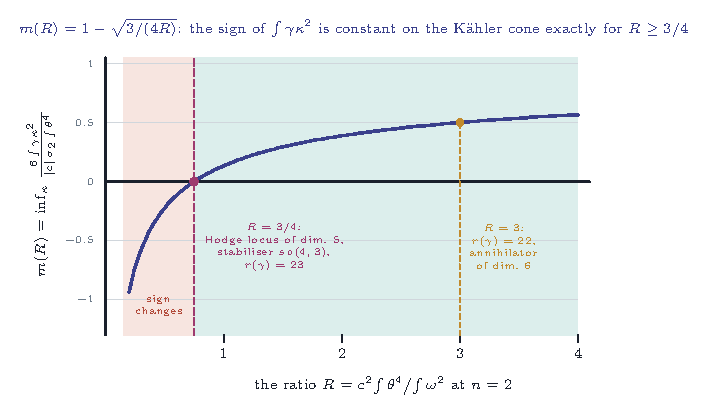
\includegraphics[width=0.86\textwidth]{fig_kahlersign}
\caption{The exceptional ratio of \Cref{rem:p2primeexceptional}. By the
identity displayed there, which is linear in $\gamma$, the infimum over the
K\"ahler cone of $6\int\gamma\kappa^{2}\big/\bigl(|c|\,\sigma_{2}(h)\int
\theta^{4}\bigr)$ is $m(R)=1-\sqrt{3/(4R)}$, approached at the boundary of the
cone by a positive hermitian form of rank two whose Pl\"ucker coordinates
satisfy $|\xi_{01}\xi_{23}|=\frac14$. It is negative exactly for $R<3/4$, and
$R=3/4$ is also where the Hodge locus of $\gamma$ jumps from dimension $4$ to
$5$ and its stabiliser becomes $\mathfrak{so}(4,3)$, with $r(\gamma)=23$; at
$R=3$ the annihilator has dimension $6$ and $r(\gamma)=22$. Items (LII)(D),
(E) and (G) check these values.}
\label{fig:kahlersign}
\end{figure}

\begin{remark}[Which obstructions survive the correction]
\label{rem:p2primesurvive}
The obstruction theorems of this section and of \Cref{sec:semireg} were
proved for a Chern character on the Weil line; for a corrected character they
divide as follows. Unchanged, with $r(\gamma)$ in place of $2n(2n-1)$ where a
number occurs: \Cref{thm:linebundle} and \Cref{cor:noline}, whose only
hypothesis is that $\ch(E)$ stay of Hodge type to first order along
$\cD_{n,n}$; \Cref{thm:positivity} and \Cref{cor:nofiltered}, since a
corrected character is a flat Hodge class in every degree;
\Cref{lem:finiteproduct}; and the first two parts of \Cref{thm:p2numerical},
which become \Cref{thm:p2primenumber}(iv). Unchanged only when
$c_{0}=\dots=c_{2n-2}=0$, so that $H^{0,2}$ still kills $\gamma$:
\Cref{thm:rankzero}, \Cref{prop:concentrated}, \Cref{cor:kernelfamily},
\Cref{thm:weakfails} and \Cref{thm:p2forces}(iii). Unchanged only when
$\ker H$ contains a vector with $w\ne0$, which needs $\rho\le2$, the vector
giving a compensated class of $P\wedge Q$ with a component in
$T_{+}\otimes T_{-}$: \Cref{thm:p2forces}(iv), \Cref{cor:p2shape} and
\Cref{thm:p2support}. Lost:
\Cref{thm:p2false}, outside \Cref{thm:p2primenumber}(v); the positivity of
$\chi(E,E)$ in \Cref{prop:objectsize} and with it \Cref{thm:p2endo}(i)--(iii),
by \Cref{prop:p2primeprofile}(ii); and \Cref{thm:nosum}. So for a general
shape, $\rho=3$, what this paper still excludes is a line bundle summand off
the polarisation line and a Chern character effective in the exponential
basis, and nothing else; \Cref{prop:scalaratiyah} below extends the first to
summands with a scalar Atiyah class. An object with no such summand, whose
Chern character is not effective, and with $\dim\Ext^{2}(E,E)=7n^{2}-2n$, is
not excluded by anything proved here, and none is known.
\end{remark}

\begin{proposition}[Summands with a scalar Atiyah class]\label{prop:scalaratiyah}
Let $A$ be of $(K,-1,n)$-Weil type with $n\ge2$, let $T=T_{[A]}\cD_{n,n}$, and
let $E$ be a perfect complex on $A$ with $v\lrcorner\ch(E)=0$ for every
$v\in T$. Suppose $E$ has a direct summand $F[p]$ with
$\mathrm{At}(F)=\delta\cdot\id_{F}$, where $\delta$ is a real class of type
$(1,1)$ that is not a real multiple of $\theta$, and $\rk F\ne0$. Then there is
$v\in T$ with $\operatorname{ev}_{E}(v)\ne0$ and
$\sigma_{E}(\operatorname{ev}_{E}(v))=0$. In particular no finite direct sum
of shifted bundles $\pi_{*}L$, $\pi$ an isogeny, among them the simple
semi-homogeneous bundles, has a corrected character $\gamma$ with $N\ne0$ and
injective semiregularity map.
\end{proposition}

\begin{proof}
As in \Cref{thm:linebundle}, $\operatorname{ev}_{E}(v)=v\lrcorner\mathrm{At}(E)$
on $H^{1}(T_{A})$ and the Atiyah class of a direct sum is block diagonal, so
the component of $\operatorname{ev}_{E}(v)$ in $\Ext^{2}(F,F)$ is
$(v\lrcorner\delta)\cdot\id_{F}$; the map $z\mapsto z\cdot\id_{F}$ on
$H^{0,2}$ is injective because $\mathrm{tr}(z\cdot\id_{F})=\rk(F)\,z$, and
some $v\in T$ has $v\lrcorner\delta\ne0$ by \Cref{prop:rigidity}(i). On the
other hand $\sigma_{E}(\operatorname{ev}_{E}(v))=v\lrcorner\ch(E)=0$. For the
last sentence, the proof of \Cref{lem:blocks}(i) gives
$\mathrm{At}(\pi_{*}L)=\delta\cdot\id$ with $\pi^{*}\delta=c_{1}(L)$ for any
line bundle $L$, and $\ch(\pi_{*}L)=\rk(\pi_{*}L)\,e^{\delta}$; if every
$\delta$ were a multiple of $\theta$ the Chern character of the sum would lie
in $\QQ[\theta]$, which does not contain $\omega$ because $\omega\theta=0$ and
$\theta^{n+1}\ne0$.
\end{proof}

\Cref{thm:semiregclosure} asks that $\sigma_{E}$ be injective. What its proof
uses is that the relative deformations of $E$ dominate the family, and
Pridham's form of \Cref{thm:BF}, in which $\sigma_{E}$ annihilates every
obstruction, gives that under a weaker hypothesis. It tolerates an object that
is obstructed to first order, which is exactly how \Cref{thm:linebundle},
\Cref{cor:noline} and \Cref{prop:scalaratiyah} fail an object.

\begin{proposition}[A flatness form of the criterion]\label{prop:p2flat}
Let $n\ge2$, $s_{0}\in\cD_{n,n}$, and let $E$ be a bounded complex of vector
bundles on $A_{s_{0}}$ with $\ch(E)=N\omega_{1}+\sum_{k}c_{k}\theta^{k}$ and
$N\ne0$. Let $K_{E}$ be the base of a miniversal deformation of $E$ on the
fixed variety $A_{s_{0}}$, put $e=\dim\Ext^{1}(E,E)$ and
$k=\dim\ker\sigma_{E}$, and grant \Cref{thm:BF} in Pridham's form, in which
$\sigma_{E}$ annihilates every obstruction, both on $A_{s_{0}}$ and along the
Artinian deformations of $A_{s_{0}}$ in $\cD_{n,n}$.
\begin{enumerate}[label=\textup{(\roman*)},leftmargin=2.6em,itemsep=2pt]
\item $\dim K_{E}\ge e-k$.
\item If $\dim K_{E}=e-k$, then $\Sigma=\cD_{n,n}$, and the Hodge conjecture
  holds in every degree for every member of the family with
  $\Hg(A)=\SU(V,H)$.
\item $\dim K_{E}=e-k$ as soon as the cone
  $\{\xi\in\Ext^{1}(E,E):\xi\circ\xi=0\}$ has codimension $k$.
\end{enumerate}
For $k=0$ this is \Cref{thm:semiregclosure}.
\end{proposition}

\begin{proof}
Let $R$ be the completed local ring of $\cD_{n,n}$ at $s_{0}$, regular of
dimension $n^{2}$. By hypothesis $\ker\sigma_{E}$ is a complete obstruction
space for the deformations of the pair $(A_{s},E)$ over Artinian $R$-algebras,
whose relative tangent space is $\Ext^{1}(E,E)$; so this functor has a hull
$P/J$ with $P=R[[x_{1},\dots,x_{e}]]$ and $J$ generated by at most $k$
elements \cite{FM98}, and its fibre over the closed point of $R$ is a hull of
the absolute functor, of dimension $\dim K_{E}$. Krull's height theorem gives
$\dim P/J\ge n^{2}+e-k$, and the same count on the fibre gives (i). If
$\dim K_{E}=e-k$, the dimension inequality for a local homomorphism
\cite[Theorem~15.1]{Mat86} gives $\dim P/J\le n^{2}+e-k$, so equality holds, $J$
has height $k$ and is generated by a regular sequence, $P/J$ is
Cohen--Macaulay, and it is flat over $R$ by miracle flatness
\cite[Theorem~23.1]{Mat86}.\footnote{A local homomorphism from a regular local
ring to a Cohen--Macaulay local ring is flat exactly when the dimension of the
target is the dimension of the source plus that of the fibre; here both sides
equal $n^{2}+e-k$.} The analytic Kuranishi germ of pairs, as in the
proof of \Cref{thm:p2false}, has $P/J$ as its completion, so it is flat over
the germ of $\cD_{n,n}$ at $s_{0}$ and therefore open onto a neighbourhood
$U$ of $s_{0}$. Every $A_{s}$ with $s\in U$ then carries a bounded complex of
vector bundles, algebraic by GAGA, whose Chern character is the parallel
transport of $\ch(E)$, so $N\omega_{1,s}$ differs from an algebraic class by a
polynomial in $\theta$ and is algebraic; \Cref{cor:allornothing} gives (ii).
For (iii), the quadratic part of the Kuranishi map of $E$ is
$\xi\mapsto\xi\circ\xi$, so the tangent cone of $K_{E}$ lies in the cone of the
hypothesis, and $\dim K_{E}\le e-k$. Every step uses only deformations along
$\cD_{n,n}$, which are projective, where \Cref{thm:p2false} needs
non-projective ones.
\end{proof}

No object is known that meets (iii) with $k>0$, and none is excluded by
anything in this paper; the proposition says only that injectivity of
$\sigma_{E}$ is more than propagation needs.

\subsection{What the object must be, and what it cannot be}
\label{ssec:whatobject}

\Cref{thm:semiregclosure} asks for one perfect complex at one base point.
The cheapest candidate is a sum of line bundles on a split member, because
there the Weil classes are already polynomials in $\beta$, $\widehat\beta$ and
$\ell$ by \Cref{thm:splitclosed}, so the Chern character one wants is
manifestly in reach. This subsection settles that candidate. It does not
exist, and the obstruction is not semiregularity: it is the Chern character
condition, and it fails because the norm form of $K$ is positive
definite.\footnote{The norm form has now closed three different doors in this
paper, by three different mechanisms, and they should be kept apart.
\Cref{thm:character} uses the norm \emph{character} of $\Kx$ and an
equivariance hypothesis. \Cref{prop:divfails} uses the fact that the part $R$
of $H^{2}$ on which $\Kx$ acts through $\tau^{2}$ and $\bbar\tau^{\,2}$ has no
Hodge classes at a general point, which is a statement about the Hodge group.
\Cref{thm:positivity} below uses neither: it uses that $\Nm_{K/\QQ}$ is a
positive definite quadratic form on $K$ and that the multiplicities of a
filtration are positive integers. The three are independent, and only the
third is available at a special point, which is exactly where the object of
\Cref{prop:ktheory} has to live.}

\begin{lemma}[The semiregularity map of a split object]\label{lem:splitsemireg}
Let $Y$ be a smooth projective complex variety and let
\[
  E=\bigoplus_{i=1}^{s}L_{i}[p_{i}]^{\oplus m_{i}},
  \qquad \lambda_{i}=c_{1}(L_{i}),
\]
with the $L_{i}$ line bundles, the $\lambda_{i}$ pairwise distinct and
$p_{i}\in\ZZ$. Then for $\zeta=(\zeta_{ij})\in\Ext^{2}(E,E)$,
\begin{equation}\label{eq:splitsigma}
  \sigma_{E}(\zeta)_{q}
  =\frac{1}{q!}\sum_{i=1}^{s}(-1)^{p_{i}}\,
    \mathrm{tr}(\zeta_{ii})\,\lambda_{i}^{\,q},
\end{equation}
so $\sigma_{E}$ annihilates $\Ext^{2}(L_{i}[p_{i}],L_{j}[p_{j}])$ for $i\ne j$
and the traceless part of each diagonal block. Consequently $\sigma_{E}$ is
injective if and only if all three of the following hold:
\begin{enumerate}[label=\textup{(\roman*)},nosep]
\item $m_{i}=1$ for every $i$;
\item $H^{\,2+p_{i}-p_{j}}\bigl(Y,L_{j}L_{i}^{-1}\bigr)=0$ for all $i\ne j$;
\item the map
  \[
    \Phi\colon H^{2}(\cO_{Y})^{\oplus s}\longrightarrow H^{*}(Y,\CC),
    \qquad
    (\zeta_{i})\longmapsto\sum_{i}e^{\lambda_{i}}\zeta_{i},
  \]
  is injective.
\end{enumerate}
\end{lemma}

\begin{proof}
The Atiyah class of a direct sum is the direct sum of the Atiyah classes, and
that of a line bundle is its first Chern class, so $\mathrm{At}(E)$ is
diagonal with entries $\lambda_{i}$ and $\mathrm{At}(E)^{q}$ is diagonal with
entries $\lambda_{i}^{\,q}$. The matrix product $\zeta\circ\mathrm{At}(E)^{q}$
therefore has $(i,j)$ entry $\zeta_{ij}\lambda_{i}^{\,q}$, and the trace keeps
only the diagonal; a shift by $p$ multiplies the trace by $(-1)^{p}$. That is
\eqref{eq:splitsigma}, and it exhibits the two spaces the map kills.

For the equivalence, the off-diagonal part of $\Ext^{2}(E,E)$ is
$\bigoplus_{i\ne j}\Ext^{2}(L_{i}[p_{i}],L_{j}[p_{j}])
=\bigoplus_{i\ne j}H^{2+p_{i}-p_{j}}(L_{j}L_{i}^{-1})$, which must vanish,
giving (ii); the diagonal block at $i$ is $H^{2}(\cO_{Y})\otimes
\mathrm{End}(\CC^{m_{i}})$ and only its trace survives, so $m_{i}=1$, giving
(i). What is left is $\bigoplus_{i}H^{2}(\cO_{Y})$, and by
\eqref{eq:splitsigma} an element $(\zeta_{i})$ of it dies exactly when
$\sum_{i}\lambda_{i}^{\,q}\zeta_{i}=0$ for every $q\ge0$, which is (iii) after
absorbing the signs $(-1)^{p_{i}}$ into the $\zeta_{i}$ and the factorials
into the grading.
\end{proof}

Condition (ii) is cheap, because the shifts $p_{i}$ are at our disposal: only
their parities are fixed by the Chern character, and a line bundle whose first
Chern class is nondegenerate of index $k$ has cohomology in degree $k$ alone,
so one may choose the $p_{i}$ to avoid every index that occurs. Condition
(iii) is a rank. Condition (i) is free. What is not free is the Chern
character itself, and that is what the rest of this subsection is about.

\begin{notation}[Coordinates on the divisor classes]\label{not:splitcoords}
Let $A_{0}=X\times\widehat{X}$ be a split member, $n\ge2$, and keep
$\gamma=d\beta-\widehat{\beta}$ from \Cref{not:threeclasses}. Write
\[
  \theta^{\pm}=\gamma\mp\sqrt{-d}\,\ell\in\textstyle\bigwedge^{2}V_{\pm},
  \qquad
  R_{0}=\QQ\gamma\oplus\QQ\ell\subset R .
\]
Every $\theta\in R_{0}$ is $\theta=u\theta^{+}+\bbar u\,\theta^{-}$ for a
unique $u\in K$, and in coordinates $u=g+h\sqrt{-d}$ corresponds to
$\theta=2g\gamma+2dh\,\ell$. By \Cref{prop:splitgeom}(iv) the group
$\NS(A_{0})_{\QQ}$ at a split member with $X$ general is
$\QQ\eta\oplus R_{0}$, so every divisor class is $e\eta+\theta$ with
$e\in\QQ$ and $\theta\in R_{0}$, and we write $u(\lambda)\in K$ for the
coordinate of its $R_{0}$-part.
\end{notation}

\begin{lemma}[A basis in degree four]\label{lem:sixmonomials}
For $n\ge2$ the six products
$\beta^{2},\widehat\beta^{2},\ell^{2},\beta\widehat\beta,\beta\ell,
\widehat\beta\ell$
are linearly independent in $H^{4}(A_{0},\QQ)$. Equivalently the six classes
$\eta^{2}$, $\eta\theta^{+}$, $\eta\theta^{-}$, $(\theta^{+})^{2}$,
$(\theta^{-})^{2}$, $\theta^{+}\theta^{-}$ are a basis of the degree four part
of the subring generated by the divisor classes.
\end{lemma}

\begin{proof}
Grade $H^{*}(A_{0},\QQ)=\bigwedge^{*}U\otimes\bigwedge^{*}U^{\vee}$ by
bidegree. Then $\beta$ has bidegree $(2,0)$, $\widehat\beta$ has $(0,2)$ and
$\ell$ has $(1,1)$, so the six products have bidegrees $(4,0)$, $(0,4)$,
$(2,2)$, $(2,2)$, $(3,1)$, $(1,3)$. All are distinct except for the pair
$\beta\widehat\beta$ and $\ell^{2}$, and those two are independent in
$\bigwedge^{2}U\otimes\bigwedge^{2}U^{\vee}$ because
$\beta\widehat\beta=\beta\otimes\widehat\beta$ is decomposable there while
$\ell^{2}=-2\sum_{i<j}(x_{i}x_{j})\otimes(\xi_{i}\xi_{j})$ has all
$\binom{2n}{2}$ terms and $\binom{2n}{2}>n$ for $n\ge2$. The second
description follows because the change of basis between the two sets of six
classes is invertible over $K$: $\eta=d\beta+\widehat\beta$ and
$\gamma=d\beta-\widehat\beta$ span the same plane as
$\beta$ and $\widehat\beta$ since $\det\begin{psmallmatrix}d&1\\
d&-1\end{psmallmatrix}=-2d\ne0$, and $\theta^{\pm}$ span the same plane
as $\gamma$ and $\ell$ over $\CC$.
\end{proof}

The next lemma says the same thing at every abelian variety of Weil type, not
only at a split member, and it says it without coordinates. It is the fact the
positivity argument really turns on.

\begin{lemma}[$\theta^{+}\theta^{-}$ is never proportional to $\eta^{2}$]
\label{lem:tensorrank}
Let $(A,\iota,\eta)$ be of $(K,-1,n)$-Weil type with $n\ge2$, and let
$0\ne\theta^{\pm}\in\bigwedge^{2}V_{\pm}$. Then $\theta^{+}\theta^{-}$ is not a
scalar multiple of $\eta^{2}$ in $H^{4}(A,\CC)$.
\end{lemma}

\begin{proof}
Both classes lie in the summand
$\bigwedge^{2}V_{+}\otimes\bigwedge^{2}V_{-}$ of $H^{4}(A,\CC)$, the isotypic
component for the character $\Nm^{2}$, so the question is one of tensor rank
there. The polarisation class $\eta$ lies in $V_{+}\otimes V_{-}$ and is the
hermitian form of \Cref{prop:weilline}, hence nondegenerate: in dual bases
$\eta=\sum_{a=1}^{2n}v_{a}\wedge w_{a}$ with $v_{a}$ a basis of $V_{+}$ and
$w_{a}$ a basis of $V_{-}$. Squaring,
\[
  \eta^{2}
  =\sum_{a,b}(v_{a}\wedge w_{a})(v_{b}\wedge w_{b})
  =-2\sum_{a<b}(v_{a}v_{b})\otimes(w_{a}w_{b}),
\]
which is diagonal in the induced bases of $\bigwedge^{2}V_{+}$ and
$\bigwedge^{2}V_{-}$ and therefore has tensor rank exactly $\binom{2n}{2}$.
The class $\theta^{+}\theta^{-}$ is, up to sign,
$\theta^{+}\otimes\theta^{-}$, of tensor rank one. For $n\ge2$ one has
$\binom{2n}{2}\ge6>1$, so the two cannot be proportional.
\end{proof}

\begin{theorem}[The positivity obstruction]\label{thm:positivity}
Let $(A,\iota,\eta)$ be of $(K,-1,n)$-Weil type with $n\ge2$, and suppose that
the only divisor classes on which $\Kx$ acts through the norm character are
the multiples of $\eta$, that is
\begin{equation}\label{eq:noextranorm}
  \NS(A)_{\QQ}\cap\bigl(V_{+}\otimes V_{-}\bigr)=\QQ\,\eta .
\end{equation}
Let $E$ be a perfect complex on $A$ whose Chern character is effective in the
exponential basis, meaning
\begin{equation}\label{eq:effectivech}
  \ch(E)=\sum_{i=1}^{s}m_{i}\,e^{\lambda_{i}},
  \qquad m_{i}\in\QQ_{>0},\quad\lambda_{i}\in\NS(A)_{\QQ},
\end{equation}
and write $\lambda_{i}=e_{i}\eta+\theta_{i}$ with $\theta_{i}$ in the part $R$
of $H^{2}(A,\QQ)$ carrying the characters $\tau^{2}$ and $\bbar\tau^{\,2}$, and
$u_{i}\in K$ for the $\theta^{+}$-coordinate of $\theta_{i}$. If $\ch_{2}(E)$
is a flat Hodge class, then
\begin{equation}\label{eq:normsum}
  \sum_{i=1}^{s}m_{i}\,\Nm_{K/\QQ}(u_{i})=0 ,
\end{equation}
and since $\Nm_{K/\QQ}$ is positive definite and every $m_{i}$ is positive,
$u_{i}=0$ for every $i$. Hence every $\lambda_{i}$ is a rational multiple of
$\eta$, and $\ch_{k}(E)\in\QQ\,\eta^{k}$ for every $k$. In particular
$\ch_{n}(E)$ has no component on the Weil line.
\end{theorem}

\begin{proof}
From \eqref{eq:effectivech},
$\ch_{2}(E)=\tfrac12\sum_{i}m_{i}\lambda_{i}^{2}$. Decompose $H^{4}(A,\CC)$
into $\Kx$-isotypic pieces and keep the one for $\Nm^{2}$, namely
$\bigwedge^{2}V_{+}\otimes\bigwedge^{2}V_{-}$. Writing
$\theta_{i}=u_{i}\theta^{+}+\bbar u_{i}\theta^{-}$ for a fixed choice of
generators $\theta^{\pm}$ of $\bigwedge^{2}V_{\pm}$, one has
\[
  \lambda_{i}^{2}
  =e_{i}^{2}\eta^{2}
   +2e_{i}\eta\theta_{i}
   +u_{i}^{2}(\theta^{+})^{2}+\bbar u_{i}^{2}(\theta^{-})^{2}
   +2\Nm_{K/\QQ}(u_{i})\,\theta^{+}\theta^{-},
\]
and of these five terms only the first and the last are in the $\Nm^{2}$
piece: $\eta\theta_{i}$ carries $\Nm\tau^{2}$ and $\Nm\bbar\tau^{\,2}$, and
$(\theta^{\pm})^{2}$ carry $\tau^{4}$ and $\bbar\tau^{\,4}$, all four distinct
from $\Nm^{2}$. Hypothesis \eqref{eq:noextranorm} is what makes the
decomposition $\lambda_{i}=e_{i}\eta+\theta_{i}$ available with $e_{i}$ a
scalar. So the $\Nm^{2}$-part of $\ch_{2}(E)$ is
\[
  \tfrac12\Bigl(\sum_{i}m_{i}e_{i}^{2}\Bigr)\eta^{2}
  +\Bigl(\sum_{i}m_{i}\Nm_{K/\QQ}(u_{i})\Bigr)\theta^{+}\theta^{-}.
\]

Now compare with the flat Hodge classes of degree four. For $n\ge3$ they are
$\QQ\eta^{2}$ by \Cref{thm:hdgcount}. For $n=2$ they are
$\QQ\eta^{2}\oplus\HW(A)$, and $\HW(A)$ spans the summands for $\tau^{4}$ and
$\bbar\tau^{\,4}$, which are not $\Nm^{2}$. In both cases the $\Nm^{2}$-part
of a flat Hodge class of degree four is a multiple of $\eta^{2}$. By
\Cref{lem:tensorrank} the class $\theta^{+}\theta^{-}$ is not such a multiple,
so its coefficient must vanish, which is \eqref{eq:normsum}.

Finally $\Nm_{K/\QQ}(g+h\sqrt{-d})=g^{2}+dh^{2}$ with $d>0$, so
$\Nm_{K/\QQ}(u)\ge0$ with equality only at $u=0$, and a sum of nonnegative
terms with positive weights vanishes only when every term does. Then
$\ch_{k}(E)=\frac{1}{k!}\bigl(\sum_{i}m_{i}e_{i}^{k}\bigr)\eta^{k}$, and
$\eta^{k}$ is not on the Weil line by \Cref{thm:hdgcount}.
\end{proof}

\begin{corollary}[The cheapest objects do not exist]\label{cor:nofiltered}
Let $A$ satisfy \eqref{eq:noextranorm}, which holds at every split member of
\Cref{thm:splitclosed} and at every quaternionic base point of
\Cref{thm:quatweil}.\footnote{At a split member $\NS(A)_{\QQ}$ has rank three
with basis $\beta,\widehat\beta,\ell$ by \Cref{prop:splitgeom}(iv), and of
these $\eta$ spans the norm-character part while $\gamma$ and $\ell$ span
$R$. At a quaternionic point $\NS(A)_{\QQ}$ is the space of Rosati-symmetric
elements of $B=(-d,b)_{\QQ}$, which is spanned by $1$, $j$ and $ij$; the first
gives $\eta$ and the other two are semilinear over $K$, hence lie in $R$. In
both cases the norm-character part of $\NS(A)_{\QQ}$ is exactly $\QQ\eta$.}
Then \Cref{thm:semiregclosure} cannot be applied at $A$ with any of the
following:
\begin{enumerate}[label=\textup{(\alph*)},nosep]
\item a coherent sheaf admitting a filtration by line bundles, in particular
  any direct sum of line bundles;
\item a simple semi-homogeneous vector bundle in the sense of Mukai
  \cite{Muk78}, since such a bundle of rank $r$ has $\ch(E)=r\,e^{c_{1}(E)/r}$;
\item any iterated extension of the objects in (a) and (b).
\end{enumerate}
In each case the failure is not of the semiregularity hypothesis but of the
Chern character hypothesis of \Cref{prop:ktheory}: no such $E$ has a Chern
character which is a flat section of Hodge classes with a nonzero Weil
component.
\end{corollary}

\begin{proof}
Each of (a), (b) and (c) has a Chern character of the shape
\eqref{eq:effectivech} with positive multiplicities, by additivity of $\ch$
along a filtration and by Mukai's computation of the Chern character of a
simple semi-homogeneous bundle. Apply \Cref{thm:positivity}.
\end{proof}

\begin{remark}[Where the theorem has force, and why it does not contradict
Markman]\label{rem:markmanpositivity}
At a very general member of the family $\NS(A)_{\QQ}=\QQ\eta$, so
\Cref{thm:positivity} is true for the empty reason that there are no
$\theta_{i}$ to begin with. Its content is at the special members, which is
exactly where \Cref{thm:semiregclosure} needs its object to live and where the
base points of \Cref{thm:everyfamily} are. That is the opposite of the usual
situation in this paper, where the special members are the easy ones.

The theorem also does not touch the objects of Markman \cite{Mar25a,Mar25b}.
Those are sheaves whose class in $K_{0}$ is not a positive combination of
exponentials of divisor classes, so \eqref{eq:effectivech} fails for them at
the first step; and they live at very general points, where as just noted the
statement is vacuous anyway. What the theorem does is remove the class of
objects one would reach for first, and it removes it for a reason which is
visible before any cohomology is computed.
\end{remark}

\begin{proof}
Immediate from \Cref{thm:positivity}, since the conclusion there contradicts
the requirement that $\ch_{n}(E)$ have a nonzero component on the Weil line.
\end{proof}

\begin{remark}[What is left of the candidate, and what it must look like]
\label{rem:whatitmustbe}
\Cref{thm:positivity} uses positivity of the multiplicities and nothing else,
so it says exactly where to go next: the object must be a complex whose
class in $K_{0}$ is not effective, that is one in which the line bundles
appear with multiplicities of both signs. Such objects exist. Writing
$E=F\oplus G[1]$ with $F$ and $G$ sums of line bundles, the class in $K_{0}$
is $[F]-[G]$ and \eqref{eq:normsum} becomes
$\sum_{L_{i}\subset F}\Nm(u_{i})=\sum_{L_{j}\subset G}\Nm(u_{j})$, which is
satisfiable; and \Cref{lem:splitsemireg} still applies verbatim, with the
shifts absorbing condition (ii).

Two further facts, both computational, say how little room is left at $n=2$,
and how much more there is beyond it. First, the map $\Phi$ of
\Cref{lem:splitsemireg}(iii) is injective at $n=2$ for $s\le3$ and, for a
general choice of $\lambda_{1},\dots,\lambda_{4}$, has rank $22$ rather than
$24$; so at $n=2$ no more than three line bundles may occur at all. This is
special to $n=2$: at $n=3$ the same map is injective for a general choice of
up to ten classes, and the dimension count permits up to $33$. Second, an
exhaustive search over the classes $a\beta+b\widehat\beta+c\ell$ with
$|a|,|b|,|c|\le3$, for $d=1$ and $d=2$, finds no signed tuple of at most
three line bundles whose Chern character is a flat section of Hodge classes
with a nonzero Weil component; the tuples of at most four that do satisfy the
Chern character condition with a nonzero Weil component, $888$ of them at
$d=1$ and $30$ at $d=2$, all have exactly four terms, and all of them fail
\Cref{lem:splitsemireg}(iii): the kernel has dimension $2$, $3$, $4$ or $6$
at $d=1$ and $3$ or $6$ at $d=2$, never $0$. Item (XIII) of
\Cref{sec:verification} carries both computations.

So the object of \Cref{thm:semiregclosure}, if it exists at a split member, is
not a sum of line bundles in any arrangement of signs and shifts: it must have
$\Ext^{2}$ that the trace does not see, that is, it must be indecomposable in
the derived category. That is a sharper description of the remaining
construction than \Cref{rem:tworemain} gives, and it is as far as we have been
able to push it.
\end{remark}

\subsection{The object, written down, and what it costs}
\label{ssec:pte}

\Cref{prop:ktheory} produced the object of \Cref{thm:semiregclosure} by an
existence argument: the Chern character is an isomorphism onto the Chow ring
with rational coefficients, so a $K$-theory class with the right character
exists. That is enough for the theorem and tells one nothing about the object.
This subsection writes it down. The answer turns the question into a
Diophantine one, and the Diophantine problem has a classical name.

\begin{setupenv}[Objects supported on $R$]\label{setup:pte}
Let $A$ be of $(K,-1,n)$-Weil type, $n\ge2$, satisfying
\eqref{eq:noextranorm}, and keep $\theta^{\pm}$ from
\Cref{not:splitcoords}. For $u\in K$ with $\theta(u)=u\theta^{+}+\bbar
u\,\theta^{-}\in\NS(A)_{\QQ}$, and for multiplicities $m_{i}\in\ZZ$, consider
\[
  v=\sum_{i=1}^{s}m_{i}\,e^{\theta(u_{i})},
  \qquad
  T_{q,r}=\sum_{i=1}^{s}m_{i}\,u_{i}^{q}\,\bbar u_{i}^{\,r}
  \quad (q,r\ge0).
\]
\end{setupenv}

\begin{proposition}[The Chern character in terms of the $u_{i}$]
\label{prop:chintermsofu}
In \Cref{setup:pte},
\begin{equation}\label{eq:chexpansion}
  v_{k}
  =\sum_{\substack{q+r=k\\ 0\le q,r\le n}}
    \frac{T_{q,r}}{q!\,r!}\,(\theta^{+})^{q}(\theta^{-})^{r},
\end{equation}
because $(\theta^{\pm})^{q}=0$ for $q>n$. Consequently $v$ is a flat section
of Hodge classes with a nonzero Weil component if
\begin{equation}\label{eq:pteconditions}
  T_{q,r}=0\ \ \text{for all } 0\le q,r\le n \text{ with }
  (q,r)\notin\{(0,0),(n,0),(0,n)\},
  \qquad T_{n,0}\ne0,
\end{equation}
and then $v_{0}=T_{0,0}=\sum_{i}m_{i}$, $v_{k}=0$ for $0<k<2n$ with $k\ne n$,
and
\[
  v_{n}=\frac{1}{n!}\Bigl(T_{n,0}(\theta^{+})^{n}
        +\bbar{T}_{n,0}(\theta^{-})^{n}\Bigr),
\]
a nonzero rational multiple of a generator of the Weil line, by
\Cref{thm:splitclosed}.
\end{proposition}

\begin{proof}
Expand $\theta(u_{i})^{k}$ by the binomial theorem, divide by $k!$ and collect;
the vanishing of $(\theta^{\pm})^{q}$ for $q>n$ is because
$\theta^{\pm}\in\bigwedge^{2}V_{\pm}$ and $\dim_{\CC}V_{\pm}=2n$. Under
\eqref{eq:pteconditions} the only surviving terms of \eqref{eq:chexpansion}
are the ones listed, and $(\theta^{+})^{n}$ spans $\bigwedge^{2n}V_{+}$, which
is the Weil line over $\CC$.
\end{proof}

So the search for the object of \Cref{thm:semiregclosure} is the search for a
finitely supported integer-valued function on $\cO_{K}$ that annihilates every
monomial $u^{q}\bbar u^{\,r}$ with $q,r\le n$ except three of them. Two things
follow at once, and they pull in opposite directions.

\begin{lemma}[Equal norms force the Prouhet--Tarry--Escott condition]
\label{lem:pte}
Suppose all the $u_{i}$ in \Cref{setup:pte} have the same norm
$N=\Nm_{K/\QQ}(u_{i})>0$. Then \eqref{eq:pteconditions} holds if and only if
\begin{equation}\label{eq:ptepure}
  \sum_{i}m_{i}u_{i}^{\,k}=0\ \ \text{for } k=0,1,\dots,n-1,
  \qquad
  \sum_{i}m_{i}u_{i}^{\,n}\ne0 .
\end{equation}
With $m_{i}=\pm1$ this says that the $u_{i}$ split into two multisets on the
circle $\Nm=N$ whose power sums agree through degree $n-1$ and differ at
degree $n$: a Prouhet--Tarry--Escott pair of degree $n-1$, constrained to a
norm circle of $\cO_{K}$.
\end{lemma}

\begin{proof}
For $q\ge r$ one has $u^{q}\bbar u^{\,r}=N^{r}u^{q-r}$, so
$T_{q,r}=N^{r}\sum_{i}m_{i}u_{i}^{\,q-r}$, and the pairs $(q,r)$ with
$q,r\le n$ realise every difference $k=q-r$ from $0$ to $n$. The excluded
pairs $(0,0)$ and $(n,0)$ are the ones with $r=0$ and $k=0$ or $k=n$; but
$k=0$ also occurs at $(1,1),\dots,(n,n)$, which are not excluded, so
$\sum_{i}m_{i}=0$ is required after all. The remaining differences
$k=1,\dots,n-1$ each occur at some non-excluded pair, and $k=n$ occurs only at
$(n,0)$.
\end{proof}

\begin{theorem}[Equal norms cannot be semiregular]\label{thm:equalnorms}
Let $E=\bigoplus_{i}L_{i}[p_{i}]$ realise \eqref{eq:ptepure} with all norms
equal. Then $\ch_{0}(E)=0$, and the semiregularity map $\sigma_{E}$ has a
kernel of dimension at least $n^{2}$.
\end{theorem}

\begin{proof}
By \Cref{lem:pte} the case $k=0$ of \eqref{eq:ptepure} gives
$\sum_{i}m_{i}=0$, which is $\ch_{0}(E)$. For the kernel, take
$\zeta_{i}=m_{i}\zeta$ for a single $\zeta\in H^{2}(\cO_{A})$; then by
\Cref{lem:splitsemireg}(iii)
\[
  \Phi\bigl((m_{i}\zeta)_{i}\bigr)
  =\Bigl(\sum_{i}m_{i}e^{\lambda_{i}}\Bigr)\zeta=\ch(E)\,\zeta ,
\]
which by \Cref{prop:chintermsofu} is a multiple of $\omega\,\zeta$ with
$\omega$ a generator of the Weil line. Now $\HW(A)_{\CC}$ is spanned by
$\bigwedge^{2n}V_{+}$ and $\bigwedge^{2n}V_{-}$, and the Weil type condition
says $\dim V_{\pm}^{0,1}=n$; writing
$H^{2}(\cO_{A})=\bigwedge^{2}(V_{+}^{0,1}\oplus V_{-}^{0,1})$, the product of
a generator of $\bigwedge^{2n}V_{+}$ with $\zeta$ kills the components of
$\zeta$ in $\bigwedge^{2}V_{+}^{0,1}$ and in
$V_{+}^{0,1}\otimes V_{-}^{0,1}$, and likewise with the roles exchanged. So
$\omega\,\zeta=0$ for every $\zeta$ in
$V_{+}^{0,1}\otimes V_{-}^{0,1}$, a space of dimension $n^{2}$, and all of
those lie in the kernel of $\Phi$.
\end{proof}

\begin{corollary}[At least $n+1$ norms]\label{cor:nplusone}
If $E$ as in \Cref{setup:pte} satisfies \eqref{eq:pteconditions} and
$\ch_{0}(E)\ne0$, then the $u_{i}$ take at least $n+1$ distinct norms.
\end{corollary}

\begin{proof}
Let $N_{1},\dots,N_{\nu}$ be the distinct norms and $M_{j}$ the sum of the
$m_{i}$ over the level $\Nm(u_{i})=N_{j}$. The conditions $T_{r,r}=0$ for
$r=1,\dots,n$ read $\sum_{j}M_{j}N_{j}^{\,r}=0$ for $r=1,\dots,n$. The matrix
$(N_{j}^{\,r})_{1\le r\le n,\,1\le j\le\nu}$ has rank $\min(n,\nu)$ because the
$N_{j}$ are distinct and nonzero, so $\nu\le n$ forces every $M_{j}=0$ and
hence $\ch_{0}(E)=\sum_{j}M_{j}=0$.
\end{proof}

\subsubsection*{The smallest solution, and what it does}

At $n=3$ and $K=\QQ(\sqrt{-3})$ the Prouhet--Tarry--Escott condition of
\Cref{lem:pte} has a solution of striking simplicity: the norm circle
$\Nm=1$ carries the six roots of unity of $K$, and the two cosets of the cube
roots of $-1$ and of $+1$ are a Prouhet--Tarry--Escott pair of degree
two.\footnote{Explicitly, with $\zeta$ a primitive sixth root of unity, the
cube roots of $-1$ are $\zeta,\zeta^{3},\zeta^{5}$ and those of $+1$ are
$1,\zeta^{2},\zeta^{4}$; each triple sums to zero and has zero sum of squares,
while the sums of cubes are $-3$ and $+3$. A search over the norm circles of
$\cO_{K}$ with $\Nm\le200$ and $|g|,|h|\le25$, for $K=\QQ(\sqrt{-d})$ with
$d=1,2,3,7$, finds this solution and its conjugate at $n=3$, one further pair
at $d=1$ and $n=4$, and nothing else; item (XIII) of \Cref{sec:verification}
records the search.}

\begin{proposition}[The object at $n=3$, written out]\label{prop:explicitobject}
Let $K=\QQ(\sqrt{-3})$, $n=3$, and let $A_{0}=X\times\widehat X$ be a split
member. In the basis $\beta,\widehat\beta,\ell$ of $\NS(A_{0})_{\QQ}$ put
\[
  \lambda_{1}=(3,-1,3),\quad
  \lambda_{2}=(-6,2,0),\quad
  \lambda_{3}=(3,-1,-3),
\]
and $\lambda_{3+i}=-\lambda_{i}$ for $i=1,2,3$, with $m_{i}=+1$ for
$i\le3$ and $m_{i}=-1$ for $i\ge4$. Then the six classes are distinct and
integral, the perfect complex
\[
  E=\bigl(L_{1}\oplus L_{2}\oplus L_{3}\bigr)\ \oplus\
    \bigl(L_{4}\oplus L_{5}\oplus L_{6}\bigr)[3]
\]
has
\[
  \ch_{k}(E)=0\ \ (k\ne3),
  \qquad
  \ch_{3}(E)=12\,\omega_{1},
\]
and every difference $\lambda_{j}-\lambda_{i}$ with $i\ne j$ is nondegenerate
of index exactly $3$, so that conditions (i) and (ii) of
\Cref{lem:splitsemireg} hold for this shift. Condition (iii) fails: the map
$\Phi$ has rank $75$ instead of $90$, with kernel of dimension
$15=\dim H^{2}(\cO_{A_{0}})$.
\end{proposition}

\begin{proof}
Everything asserted is a finite exact computation, carried out in item (XIII)
of \Cref{sec:verification}. The classes are the images under
$\theta(u)=2g\gamma+2dh\,\ell$, $u=g+h\sqrt{-3}$, of the six roots of unity
of $K$ scaled by $2$; the Chern character is \Cref{prop:chintermsofu} with the
Prouhet--Tarry--Escott data above; the index computation and the rank of
$\Phi$ are the two remaining items. For the shift, condition (ii) asks that
$2+p_{i}-p_{j}\ne3$ whenever $i\ne j$, that is $p_{i}-p_{j}\ne1$; within each
of the two blocks the difference is $0$, and between them it is $\pm3$.
\end{proof}

\begin{remark}[What this settles and what it does not]\label{rem:pteoutcome}
Three things are settled. The object of \Cref{prop:ktheory} is not an
abstraction: at $n=3$ over $\QQ(\sqrt{-3})$ it is six line bundles and a
shift, and its Chern character is exactly $12$ times a Weil class with every
other graded piece zero. The construction is completely general, and
\Cref{lem:pte} identifies the constraint as a Prouhet--Tarry--Escott problem
on a norm circle, which is a question of a kind that can be attacked. And
\Cref{cor:nplusone} says what any semiregular solution must look like: the
$u_{i}$ must take at least $n+1$ distinct norms, because otherwise the rank is
zero and \Cref{thm:equalnorms} produces a kernel of dimension $n^{2}$.

The remaining question was the existence of a solution with $n+1$ norms. The
level sums are then forced up to scale, and they compete with the supply of
elements of $\cO_{K}$ at each level; \Cref{thm:pterange} carries out that
competition in a range, and \Cref{cor:noline} then shows that no solution in
any range could have served, because a line bundle summand off the
polarisation line is obstructed along the family whatever the norms.
\end{remark}

\subsubsection*{The obstruction classes of the explicit object}

\Cref{cor:kernelfamily} and \Cref{rem:whatmeasures} say that the kernel of
$\sigma_{E}$ contains a copy of the tangent space of the Weil family, and
that this is a statement about where the semiregularity map is blind, not a
statement that the object is obstructed. For the explicit object the
obstruction classes can be written down, and they are not zero. The
computation is elementary and we record it in general.

Recall the conventions of \Cref{ssec:tangent}: a first-order deformation of
$A$ is $v\in\Hom(H^{1,0},H^{0,1})=H^{1}(A,T_{A})$, extended by zero on
$H^{0,1}$ and acting on $H^{*}(A,\CC)$ as a derivation $v\lrcorner$; a class
$\xi$ of type $(p,p)$ stays of type $(p,p)$ to first order along $v$ exactly
when $v\lrcorner\,\xi=0$. For a line bundle $L$ with $\lambda=c_{1}(L)$ the
Atiyah class is $\lambda\in H^{1}(\Omega^{1}_{A})$, its contraction with $v$
is $v\lrcorner\,\lambda\in H^{2}(\cO_{A})=H^{0,2}(A)$, and this is the
obstruction to deforming $L$ along $v$; a shift does not change it. For
$E=\bigoplus_{i}L_{i}[p_{i}]$ the Atiyah class is diagonal with entries
$\lambda_{i}$, as in the proof of \Cref{lem:splitsemireg}, so the
obstruction to deforming $E$ along $v$ is the diagonal element
\begin{equation}\label{eq:obdef}
  \ob_{E}(v)=\bigl(v\lrcorner\,\lambda_{i}\bigr)_{i}
  \in\bigoplus_{i}H^{0,2}(A)\subset\Ext^{2}(E,E).
\end{equation}

\begin{proposition}[The obstruction map of a split object]
\label{prop:splitobstruction}
Let $A_{0}=X\times\widehat X$ be a split member with $\beta$ principal and
$X$ general, so that $\NS(A_{0})_{\QQ}=\langle\beta,\widehat\beta,\ell\rangle$
by \Cref{prop:splitgeom}(iv). Let $T=T_{[A_{0}]}\cD_{n,n}$ be the space of
polarised first-order deformations commuting with $K$, of dimension $n^{2}$
by \Cref{prop:firstorder}, and put
\[
  T_{\mathrm{spl}}
  =\bigl\{\,v\in\Hom(H^{1,0},H^{0,1})\;:\;
    v\lrcorner\,\beta=v\lrcorner\,\widehat\beta=v\lrcorner\,\ell=0\,\bigr\}.
\]
Let $E=\bigoplus_{i=1}^{s}L_{i}[p_{i}]$ with $\lambda_{i}=c_{1}(L_{i})$ and
let $\ob_{E}\colon T\to\bigoplus_{i}H^{0,2}(A_{0})$ be the map
\eqref{eq:obdef} restricted to $T$.
\begin{enumerate}[label=\textup{(\roman*)},nosep]
\item $T_{\mathrm{spl}}$ is the tangent space to the split locus: it has
  dimension $n(n+1)/2$, it is contained in $T$, and it consists of the
  deformations of $X\times\widehat X$ induced by the polarised deformations
  of $(X,\beta)$.
\item If the classes $\lambda_{i}$ together with $\eta$ span
  $\NS(A_{0})_{\QQ}$, then $\ker\ob_{E}=T_{\mathrm{spl}}$ and
  $\operatorname{rank}\ob_{E}=n(n-1)/2$, the codimension of the split locus
  in $\cD_{n,n}$.
\item If $\ch_{k}(E)\in\QQ\eta^{k}$ for $k\ne n$ and
  $\ch_{n}(E)\in\QQ\eta^{n}\oplus\HW(A_{0})$, then
  $\sigma_{E}\circ\ob_{E}=0$ on $T$: for every $v\in T$,
  \begin{equation}\label{eq:sigmaob}
    \sigma_{E}\bigl(\ob_{E}(v)\bigr)=v\lrcorner\,\ch(E)=0 .
  \end{equation}
\item For the object of \Cref{prop:explicitobject}, at $n=3$ and
  $K=\QQ(\sqrt{-3})$: $\ker\ob_{E}=T_{\mathrm{spl}}$ has dimension $6$ and
  $\ob_{E}$ has rank $3$; the image of $\ob_{E}$ lies in $\ker\sigma_{E}$;
  the subspace $\Delta=\{z\cdot\id_{E}:z\in\Ann_{H^{0,2}}(\omega_{1})\}$ of
  \Cref{cor:kernelfamily} has dimension $9$ and meets the image of $\ob_{E}$
  only in zero, so that $\Delta\oplus\image\ob_{E}$ is a twelve-dimensional
  subspace of the fifteen-dimensional kernel of $\sigma_{E}$; and
  $\ob_{E}(v)$ has components $v\lrcorner\,\lambda_{i}$ on $L_{i}$ and
  $-v\lrcorner\,\lambda_{i}$ on $L_{i}^{-1}[3]$, so it lies on the line of
  vectors of the shape $(z,\dots,z)$ only when it vanishes. In particular
  $E$ has a nonzero first-order obstruction along every $v\in T$ not tangent
  to the split locus, and no element $z\cdot\id_{E}$ of $\Ext^{2}(E,E)$
  cancels it.
\end{enumerate}
\end{proposition}

\begin{proof}
(i) Let $P=H^{1,0}(X)\subset H^{1}(X,\CC)=U^{\vee}_{\CC}$ with basis
$p_{1},\dots,p_{n}$, so that $p_{1},\dots,p_{n},\bbar p_{1},\dots,\bbar p_{n}$
is a basis of $U^{\vee}_{\CC}$, and let $q_{a},\bbar q_{a}$ be the dual basis
of $U_{\CC}=H^{1}(\widehat X,\CC)$; the dual of a conjugate basis is the
conjugate of the dual basis, so the notation is consistent. The Poincar\'e
class is the identity element of $U^{\vee}\otimes U$,
\[
  \ell=\sum_{a=1}^{n}\bigl(p_{a}\wedge q_{a}+\bbar p_{a}\wedge\bbar q_{a}\bigr),
\]
and it is of type $(1,1)$, which forces $H^{1,0}(\widehat X)=\langle\bbar
q_{a}\rangle$ and $H^{0,1}(\widehat X)=\langle q_{a}\rangle$: the Hodge
structure of $\widehat X$ is the dual one. Since $\beta$ is of type $(1,1)$
and nondegenerate, $\beta=\sum_{a,b}h_{ab}\,p_{a}\wedge\bbar p_{b}$ with
$h\in\GL_{n}(\CC)$; and since $\beta$ is principal with Gram matrix $B$ in a
symplectic basis of $U$ and $\widehat\beta$ has Gram matrix $B=-B^{-1}$ in
the dual basis of $U^{\vee}$, the Gram matrix of $\widehat\beta$ in the
basis $p_{a},\bbar p_{a}$ is minus the inverse of the Gram matrix
$\begin{psmallmatrix}0&h\\-h^{\top}&0\end{psmallmatrix}$ of $\beta$ in the
basis $q_{a},\bbar q_{a}$, which gives
$\widehat\beta=-\sum_{a,b}(h^{-1})_{ab}\,\bbar q_{a}\wedge q_{b}$.

Now $H^{1,0}(A_{0})=\langle p_{a}\rangle\oplus\langle\bbar q_{a}\rangle$ and
$H^{0,1}(A_{0})=\langle\bbar p_{a}\rangle\oplus\langle q_{a}\rangle$, so a
deformation $v$ is four $n\times n$ matrices,
\[
  v(p_{a})=\sum_{c}\bigl(A_{ca}\,\bbar p_{c}+C_{ca}\,q_{c}\bigr),
  \qquad
  v(\bbar q_{a})=\sum_{c}\bigl(B_{ca}\,\bbar p_{c}+D_{ca}\,q_{c}\bigr),
\]
and $v$ kills $\bbar p_{a}$ and $q_{a}$. Contracting,
\[
  v\lrcorner\,\ell
  =\sum_{a,c}\Bigl(A_{ca}\,\bbar p_{c}\wedge q_{a}+C_{ca}\,q_{c}\wedge q_{a}
   +B_{ca}\,\bbar p_{a}\wedge\bbar p_{c}+D_{ca}\,\bbar p_{a}\wedge q_{c}\Bigr),
\]
and reading off the three kinds of monomials, $v\lrcorner\,\ell=0$ if and only
if $D=-A^{\top}$ and $B$, $C$ are symmetric. Next
\[
  v\lrcorner\,\beta
  =\sum_{a,b,c}h_{ab}\Bigl(A_{ca}\,\bbar p_{c}\wedge\bbar p_{b}
   +C_{ca}\,q_{c}\wedge\bbar p_{b}\Bigr),
\]
so $v\lrcorner\,\beta=0$ if and only if $Ch=0$, that is $C=0$, and $Ah$ is
symmetric. Likewise $v\lrcorner\,\widehat\beta=0$ if and only if $B=0$ and
$Dh^{-1}$ is symmetric. Given $D=-A^{\top}$, the last condition reads
$A^{\top}h^{-1}=h^{-\top}A$, which after multiplication by $h^{\top}$ on the
left and by $h$ on the right is $h^{\top}A^{\top}=Ah$, the symmetry of $Ah$
again. Hence
\[
  T_{\mathrm{spl}}=\bigl\{(A,B,C,D)=(A,0,0,-A^{\top})\;:\;Ah\ \text{symmetric}\bigr\},
\]
of dimension $n(n+1)/2$. It is the tangent space to the split locus: the
same computation on $X$ alone shows that the polarised first-order
deformations of $(X,\beta)$ are the matrices $A$ with $Ah$ symmetric, the
space $T_{[X]}\cA_{n}$ of dimension $n(n+1)/2$; the deformation of
$\widehat X$ induced by $A$ is the dual one, $-A^{\top}$; and the map
$A\mapsto(A,0,0,-A^{\top})$ is injective. Finally $T_{\mathrm{spl}}\subseteq
T$: for $v\in T_{\mathrm{spl}}$, $v\lrcorner\,\eta=0$ because
$\eta\in\langle\beta,\widehat\beta\rangle$, so $v$ is polarised, and
$v\lrcorner\,\omega_{1}=v\lrcorner\,\omega_{2}=0$ because $\omega_{1}$ and
$\omega_{2}$ are polynomials in $\beta,\widehat\beta,\ell$ by
\Cref{thm:splitclosed} and $v\lrcorner$ is a derivation; by
\Cref{prop:firstorder} such a $v$ commutes with $K$.

(ii) Every $v\in T$ has $v\lrcorner\,\eta=0$. If the $\lambda_{i}$ and
$\eta$ span $\NS(A_{0})_{\QQ}=\langle\beta,\widehat\beta,\ell\rangle$, then
$v\lrcorner\,\lambda_{i}=0$ for all $i$ is equivalent, for $v\in T$, to
$v\lrcorner\,\beta=v\lrcorner\,\widehat\beta=v\lrcorner\,\ell=0$, so
$\ker\ob_{E}=T\cap T_{\mathrm{spl}}=T_{\mathrm{spl}}$ by (i), and the rank
is $n^{2}-n(n+1)/2=n(n-1)/2$, which is the codimension of
\Cref{prop:splitgeom}(iii).

(iii) By \eqref{eq:splitsigma}, $\sigma_{E}(\zeta)=\sum_{i}(-1)^{p_{i}}
\zeta_{ii}\,e^{\lambda_{i}}$ for a diagonal $\zeta$. Since $v\lrcorner$ is a
derivation and $v\lrcorner\,\lambda_{i}$ has even degree,
$v\lrcorner\,\lambda_{i}^{\,q}=q\,\lambda_{i}^{\,q-1}(v\lrcorner\,\lambda_{i})$
and so $v\lrcorner\,e^{\lambda_{i}}=(v\lrcorner\,\lambda_{i})\,e^{\lambda_{i}}$.
Therefore
\[
  \sigma_{E}\bigl(\ob_{E}(v)\bigr)
  =\sum_{i}(-1)^{p_{i}}(v\lrcorner\,\lambda_{i})\,e^{\lambda_{i}}
  =v\lrcorner\sum_{i}(-1)^{p_{i}}e^{\lambda_{i}}
  =v\lrcorner\,\ch(E).
\]
For $v\in T$ one has $v\lrcorner\,\eta^{k}=k\eta^{k-1}(v\lrcorner\,\eta)=0$,
and $v\lrcorner\,\omega=0$ for every $\omega\in\HW(A_{0})$ by
\Cref{prop:firstorder}; under the hypothesis on $\ch(E)$ this gives
\eqref{eq:sigmaob}.

(iv) The three classes $\lambda_{1}=\gamma+3\ell$, $\lambda_{2}=-2\gamma$,
$\lambda_{3}=\gamma-3\ell$ span $\langle\gamma,\ell\rangle$, and
$\langle\eta,\gamma\rangle=\langle\beta,\widehat\beta\rangle$ by the
determinant in the proof of \Cref{lem:sixmonomials}, so (ii) applies and
gives the kernel and the rank; \Cref{prop:explicitobject} gives the
hypothesis of (iii), so the image lies in $\ker\sigma_{E}$. The subspace
$\Delta$ has dimension $\dim\Ann_{H^{0,2}}(\omega_{1})=n^{2}=9$ by
\Cref{lem:annihilator}. The components of $\ob_{E}(v)$ on $L_{i}$ and on
$L_{i}^{-1}[3]$ are $v\lrcorner\,\lambda_{i}$ and
$v\lrcorner\,(-\lambda_{i})=-v\lrcorner\,\lambda_{i}$, so an element of the
image of the shape $(z,\dots,z)$ has $z=-z$, hence is zero; this is
$\Delta\cap\image\ob_{E}=0$, and with $\dim\ker\sigma_{E}=15$ from
\Cref{prop:explicitobject} the dimension count follows. Every number in (iv)
is also computed directly in item (XXV) of \Cref{sec:verification}, in the
model of item (XIII).
\end{proof}

\begin{remark}[What the obstruction classes say]\label{rem:obstructionmeaning}
\Cref{prop:splitobstruction} sharpens \Cref{rem:whatmeasures} in one
direction and closes a door in another. The direction: for the explicit
object the obstruction classes along the family are nonzero, and they are
nonzero exactly in the $n(n-1)/2$ directions normal to the split locus,
which are the directions in which the Weil class has to be transported.
The door: those classes lie in the kernel of $\sigma_{E}$ by
\eqref{eq:sigmaob}, and \eqref{eq:sigmaob} holds for every object whose
Chern character is a flat section of Hodge classes along the family, so the
semiregularity map cannot detect the obstruction of any such object. The
obstruction is therefore genuine, and it is invisible to the criterion. For
the explicit object the situation is the worst possible: the twelve
dimensions $\Delta\oplus\image\ob_{E}$ of the kernel are accounted for by
the two mechanisms of \Cref{cor:kernelfamily} and \eqref{eq:obdef}, the
remaining three lie on the even side of \Cref{cor:pteobstructed} as well,
and none of the fifteen is an artefact. The classes of the shape
$z\cdot\id_{E}$ are the ones a change of the twisting class would
contribute, one and the same $z$ to every rank one summand; the last
assertion of (iv) says that no such change removes the obstruction. So the
explicit object does not move off the split locus to first order, as a
complex and as a twisted complex, and the question of \Cref{q:residual} for
it is not one of verifying a hypothesis but of replacing the object.

The positive content is the recipe. By (ii), a split object whose classes
span $\NS(A_{0})_{\QQ}$ with $\eta$ has obstruction map of rank
$n(n-1)/2$ against the family, and the spanning hypothesis is more than is
needed: in the model of item (XXV) a single class $\theta\in\NS(A_{0})_{\QQ}$
not proportional to $\eta$ already has $\{v\in T:v\lrcorner\,\theta=0\}=
T_{\mathrm{spl}}$, for each of the seven classes tested at
$(n,d)=(2,1),(2,3),(3,3)$. So every split object built from line bundles
other than powers of $\eta$ is obstructed in exactly the normal directions
to the split locus, and \Cref{thm:positivity} says that an object built
from powers of $\eta$ carries no Weil class. What survives is the statement
of \Cref{rem:familyuniform}: the object must have positive rank.
\end{remark}

\subsubsection*{The evaluation map of the explicit object}

\Cref{thm:weakfails} places the copy $\Delta$ of the tangent space inside the
image of the evaluation map. For a split object the whole of
$\operatorname{ev}_{E}$ can be written down, and for the explicit object the
entire kernel of $\sigma_{E}$ turns out to lie in its image. We identify
$HH^{2}(A_{0})$ with
\begin{equation}\label{eq:HT2}
  HT^{2}(A_{0})
  =H^{0,2}(A_{0})\;\oplus\;\Hom\bigl(H^{1,0},H^{0,1}\bigr)\;\oplus\;
   \textstyle\bigwedge^{2}\bigl(H^{1,0}\bigr)^{\vee}
\end{equation}
by the Hochschild--Kostant--Rosenberg isomorphism, the three summands being
$H^{2}(\cO)$, $H^{1}(T)$ and $H^{0}(\bigwedge^{2}T)$ for the trivial tangent
bundle. An element $x=(z,v,\pi)$ acts on $H^{*}(A_{0},\CC)$ by $z\wedge$, by
the derivation $v\lrcorner$ of \Cref{ssec:tangent}, and by the double
contraction $\pi\lrcorner$, which removes two $(1,0)$ slots; we write
$x\lrcorner\,\xi$ for the sum of the three.%
\footnote{The double contraction is a second order operator. For a class
$\lambda$ of type $(1,1)$, which has a single $(1,0)$ slot,
$\pi\lrcorner\,\lambda=0$ and $\pi\lrcorner\,\lambda^{k}=\binom{k}{2}
\lambda^{k-2}\,(\pi\lrcorner\,\lambda^{2})$, because $\pi\lrcorner$ is a
composite of two interior products, each of which is an antiderivation, and
the only nonzero terms are those in which the two interior products hit two
different factors. Summing over $k$ with the factorials gives
$\pi\lrcorner\,e^{\lambda}=\tfrac12(\pi\lrcorner\,\lambda^{2})\,e^{\lambda}$,
exactly parallel to $v\lrcorner\,e^{\lambda}=(v\lrcorner\,\lambda)\,e^{\lambda}$
for the first order operator $v\lrcorner$. This is the whole content of the
compatibility \eqref{eq:sigmaev} below: the semiregularity map of a line
bundle is multiplication by $e^{\lambda}$, and every summand of $HT^{2}$ acts
on $e^{\lambda}$ by a scalar-valued factor which is precisely the value of
$\operatorname{ev}_{L}$. The same identity, for arbitrary $E$, is the
commutative square of Buchweitz and Flenner \cite[Corollary 4.3]{BF03} and
its Hochschild form in \cite[Lemma 11.3]{Mar25b}; on an abelian variety the
Todd class is trivial and no correction to the HKR map is needed
\cite{Cal05,BF08}.}

\begin{proposition}[The evaluation map of a split object]\label{prop:evaluation}
Let $A_{0}$ be a split member with $X$ general and let
$E=\bigoplus_{i=1}^{s}L_{i}[p_{i}]$ with $\lambda_{i}=c_{1}(L_{i})$ and all
$\Ext^{2}(L_{i}[p_{i}],L_{j}[p_{j}])$, $i\ne j$, zero, so that
$\Ext^{2}(E,E)=\bigoplus_{i}H^{0,2}(A_{0})$.
\begin{enumerate}[label=\textup{(\roman*)},nosep]
\item Under \eqref{eq:HT2}, $\operatorname{ev}_{E}$ is diagonal:
  \begin{equation}\label{eq:evsplit}
    \operatorname{ev}_{E}(z,v,\pi)_{i}
    =z+v\lrcorner\,\lambda_{i}+\tfrac12\,\pi\lrcorner\,\lambda_{i}^{2}
    \;\in\;H^{0,2}(A_{0})=\Ext^{2}\bigl(L_{i}[p_{i}],L_{i}[p_{i}]\bigr).
  \end{equation}
\item For every $x\in HT^{2}(A_{0})$,
  \begin{equation}\label{eq:sigmaev}
    \sigma_{E}\bigl(\operatorname{ev}_{E}(x)\bigr)=x\lrcorner\,\ch(E),
  \end{equation}
  and consequently
  $\ker\sigma_{E}\cap\image\operatorname{ev}_{E}
   =\operatorname{ev}_{E}\bigl(\{x:x\lrcorner\,\ch(E)=0\}\bigr)$.
  The weakened hypothesis of \cite[Question 11.4]{Mar25b} holds for $E$ if
  and only if $\operatorname{ev}_{E}$ kills every $x$ that preserves
  $\ch(E)$ to first order.
\item $\dim HT^{2}(A_{0})=2\binom{2n}{2}+4n^{2}$ and
  $\dim\Ext^{2}(E,E)=s\binom{2n}{2}$; for $s\ge5$ and every $n\ge2$ the
  second exceeds the first, so $\operatorname{ev}_{E}$ is not surjective and
  \cite[Lemma 11.3]{Mar25b} cannot apply to a sum of five or more line
  bundles.
\item For the object of \Cref{prop:explicitobject}, with
  $\lambda_{i}=u_{i}\theta^{+}+\bbar u_{i}\theta^{-}$ as in
  \Cref{not:splitcoords}: the space $\{x:x\lrcorner\,\ch(E)=0\}$ is
  $\Ann_{H^{0,2}}(\omega_{1})\oplus\{v:v\lrcorner\,\omega_{1}=0\}\oplus
  \{\pi:\pi\lrcorner\,\omega_{1}=0\}$, of dimensions $9$, $18$ and $9$; the
  first and the third summands are both carried by $\operatorname{ev}_{E}$
  onto $\Delta$; the second is carried onto
  \[
    \Sigma=\bigl\{\,(u_{i}a+\bbar u_{i}b)_{i=1}^{6}\;:\;
      a\in\textstyle\bigwedge^{2}V_{+}^{0,1},\ b\in\bigwedge^{2}V_{-}^{0,1}\,\bigr\},
    \qquad \dim\Sigma=n(n-1)=6,
  \]
  which contains the image of the obstruction map of
  \Cref{prop:splitobstruction}; $\Delta\cap\Sigma=0$; and
  \[
    \ker\sigma_{E}=\Delta\oplus\Sigma\subseteq\image\operatorname{ev}_{E}.
  \]
  So every direction in which $\sigma_{E}$ is blind is the value of
  $\operatorname{ev}_{E}$ on a Hochschild class that preserves $\ch(E)$ to
  first order, and the weakened hypothesis fails for $E$ by all fifteen
  dimensions. The rank of $\operatorname{ev}_{E}$ is $45$. The same
  containment $\ker\sigma_{E}\subseteq\image\operatorname{ev}_{E}$, with
  $\dim\ker\sigma_{E}=15$, holds for each of the eighteen configurations of
  \Cref{rem:familyuniform}.
\end{enumerate}
\end{proposition}

\begin{proof}
(i) The evaluation map is the action of $HH^{*}(A_{0})$ on
$\Ext^{*}(E,E)$, which under HKR is contraction of a polyvector in
$H^{q}(\bigwedge^{p}T)$ with $\tfrac{1}{p!}\mathrm{At}(E)^{p}$
\cite{BF08}; for $p=0$ this is $z\cdot\id_{E}$ as in the proof of
\Cref{thm:weakfails}, for $p=1$ it is $v\lrcorner\,\mathrm{At}(E)$, the map
\eqref{eq:obdef}, and for $p=2$ it is $\tfrac12\pi\lrcorner\,\mathrm{At}(E)^{2}$.
The Atiyah class of $E$ is diagonal with entries $\lambda_{i}$, so all three
are diagonal with the entries displayed.

(ii) By \eqref{eq:splitsigma}, $\sigma_{E}(\zeta)=\sum_{i}(-1)^{p_{i}}\zeta_{i}
e^{\lambda_{i}}$ for diagonal $\zeta$. The three factors in \eqref{eq:evsplit}
are exactly the scalars by which $z\wedge$, $v\lrcorner$ and $\pi\lrcorner$
act on $e^{\lambda_{i}}$: the first trivially, the second because
$v\lrcorner$ is a derivation and $v\lrcorner\,\lambda_{i}$ has even degree,
the third by the footnote above. Hence
$\sigma_{E}(\operatorname{ev}_{E}(x))=\sum_{i}(-1)^{p_{i}}\,x\lrcorner\,
e^{\lambda_{i}}=x\lrcorner\,\ch(E)$. The description of
$\ker\sigma_{E}\cap\image\operatorname{ev}_{E}$ follows: $\operatorname{ev}_{E}(x)$
lies in $\ker\sigma_{E}$ if and only if $x\lrcorner\,\ch(E)=0$.

(iii) The three summands of \eqref{eq:HT2} have dimensions $\binom{2n}{2}$,
$4n^{2}$ and $\binom{2n}{2}$. The inequality
$s\binom{2n}{2}>2\binom{2n}{2}+4n^{2}$ is $(s-2)(2n-1)>4n$, and
$4n/(2n-1)\le8/3$ for $n\ge2$, so it holds for $s\ge5$; it is checked for
$2\le n\le30$ and $5\le s\le40$ in \Cref{sec:lean}.

(iv) Since $\ch(E)=12\omega_{1}$ is of type $(3,3)$, the three summands of
$x\lrcorner\,\ch(E)$ have types $(3,5)$, $(2,4)$ and $(1,3)$, so the kernel
is the direct sum of the three kernels. The first is $\Ann_{H^{0,2}}(\omega_{1})$,
of dimension $n^{2}=9$ by \Cref{lem:annihilator}. The second is
$\Hom(V_{+}^{1,0},V_{+}^{0,1})\oplus\Hom(V_{-}^{1,0},V_{-}^{0,1})$, of
dimension $2n^{2}=18$, by the proof of \Cref{prop:firstorder}, whose
argument for (i)$\Leftrightarrow$(iii) does not use the polarisation. For the
third, decompose $\bigwedge^{2}(H^{1,0})^{\vee}$ as
$\bigwedge^{2}(V_{+}^{1,0})^{\vee}\oplus(V_{+}^{1,0})^{\vee}\otimes(V_{-}^{1,0})^{\vee}
\oplus\bigwedge^{2}(V_{-}^{1,0})^{\vee}$; here $\omega_{1}$ is a combination
of $(\theta^{+})^{3}$ and $(\theta^{-})^{3}$ with both coefficients nonzero,
$(\theta^{\pm})^{3}$ spans $\bigwedge^{3}V_{\pm}^{1,0}\otimes\bigwedge^{3}V_{\pm}^{0,1}$,
the outer blocks of $\pi$ act injectively on the respective factor
$\bigwedge^{3}V_{\pm}^{1,0}$ and land in different summands of $H^{1,3}$,
and the middle block kills both; so the third kernel is the middle block,
of dimension $n^{2}=9$.

At a split point $\theta^{\pm}$ are of type $(1,1)$, so $\theta^{\pm}\in
V_{\pm}^{1,0}\otimes V_{\pm}^{0,1}$, and they are nondegenerate pairings
because $(\theta^{\pm})^{3}\ne0$. Write $\lambda_{i}^{2}=u_{i}^{2}(\theta^{+})^{2}
+\bbar u_{i}^{2}(\theta^{-})^{2}+2\Nm(u_{i})\,\theta^{+}\theta^{-}$. A middle
block $\pi$ kills $(\theta^{\pm})^{2}$, which have no $V_{\mp}^{1,0}$ slot, so
$\tfrac12\pi\lrcorner\,\lambda_{i}^{2}=\Nm(u_{i})\,\pi\lrcorner\,(\theta^{+}\theta^{-})$;
the six $u_{i}$ of \Cref{prop:explicitobject} are $\pm\zeta_{6},\pm1,
\pm\zeta_{6}^{-1}$, all of norm one, so this value is independent of $i$ and
$\operatorname{ev}_{E}(\pi)=z_{\pi}\cdot\id_{E}$ with
$z_{\pi}=\pi\lrcorner\,(\theta^{+}\theta^{-})$. The map $\pi\mapsto z_{\pi}$
from the middle block to $V_{+}^{0,1}\otimes V_{-}^{0,1}$ is the tensor
product of the two nondegenerate pairings, hence an isomorphism onto the
middle block of $H^{0,2}$, which is $\Ann_{H^{0,2}}(\omega_{1})$ by
\Cref{lem:annihilator}. So $\operatorname{ev}_{E}$ carries the third kernel
onto $\Delta$, as it carries the first by \Cref{thm:weakfails}.

For $v=(v_{+},v_{-})$ in the second kernel,
$v\lrcorner\,\lambda_{i}=u_{i}\,v_{+}\lrcorner\,\theta^{+}+\bbar u_{i}\,
v_{-}\lrcorner\,\theta^{-}$ with $a=v_{+}\lrcorner\,\theta^{+}\in
\bigwedge^{2}V_{+}^{0,1}$ and $b=v_{-}\lrcorner\,\theta^{-}\in\bigwedge^{2}V_{-}^{0,1}$;
as $v_{\pm}$ ranges over $\Hom(V_{\pm}^{1,0},V_{\pm}^{0,1})$, $a$ and $b$
range over the whole of $\bigwedge^{2}V_{\pm}^{0,1}$ because the pairings
$\theta^{\pm}$ are nondegenerate, which is the surjectivity of
$\operatorname{alt}(Vc)$ in \eqref{eq:phidelta}. So the image is $\Sigma$.
The map $(a,b)\mapsto(u_{i}a+\bbar u_{i}b)_{i}$ is injective, because
$(u_{1},\bbar u_{1})$ and $(u_{2},\bbar u_{2})$ are linearly independent in
$\CC^{2}$, $u_{1}/\bbar u_{1}=\zeta_{6}^{2}$ differing from
$u_{2}/\bbar u_{2}=1$; hence $\dim\Sigma=2\binom{n}{2}=n(n-1)=6$. The
obstruction map of \Cref{prop:splitobstruction} is the restriction to the
polarised $K$-commuting $v$, so its image lies in $\Sigma$. An element of
$\Sigma$ of the shape $(z,\dots,z)$ has $u_{i}a+\bbar u_{i}b=z=-z$ on
comparing $i$ with $3+i$, so $z=0$ and then $a=b=0$: $\Delta\cap\Sigma=0$.
By (ii), $\Delta\oplus\Sigma\subseteq\ker\sigma_{E}\cap\image\operatorname{ev}_{E}$,
and its dimension $9+6=15$ equals $\dim\ker\sigma_{E}$ by
\Cref{prop:explicitobject}, so the three spaces coincide. The rank of
$\operatorname{ev}_{E}$ and the statement for the eighteen configurations
are the computations of item (XXVI) of \Cref{sec:verification}, which also
recomputes every dimension in this proof in the model of item (XIII).
\end{proof}

\begin{figure}[tbp]
\centering
  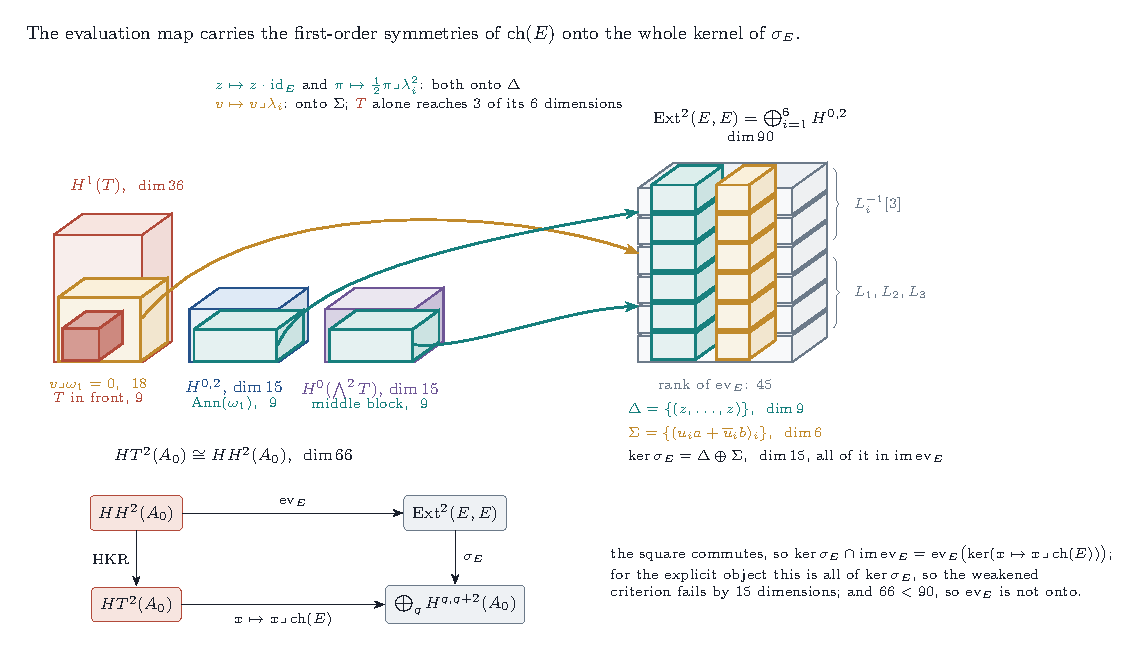
\includegraphics[width=\textwidth]{fig_evaluation}
\caption{\Cref{prop:evaluation} for the explicit object at $n=3$. Left: the
three summands of $HT^{2}(A_{0})$, drawn with heights proportional to their
dimensions, and inside each the part that preserves $\ch(E)$ to first order:
the annihilator of $\omega_{1}$, the deformations killing $\omega_{1}$ with
the polarised $K$-commuting tangent space $T$ in front, and the middle block
of bivectors. Right: $\Ext^{2}(E,E)$ as six stacked copies of $H^{0,2}$, one
per summand of $E$, and inside it the kernel of $\sigma_{E}$: the column
$\Delta$, one and the same class in every layer, and the column $\Sigma$,
whose entries depend on the summand through $u_{i}$. The three arrows are the
evaluation map on the three kernels; the two teal ones both land on
$\Delta$, the ochre one on $\Sigma$, and together they cover the kernel.
Below, the commutative square that makes this a statement about the weakened
criterion of \cite[Question 11.4]{Mar25b}.}
\label{fig:evaluation}
\end{figure}

\begin{remark}[Question 11.4 for split objects, and what is left of it]
\label{rem:question114}
For a split object the two criteria stand or fall together, and for the
explicit object both fall completely. \Cref{thm:weakfails} makes the first
$n^{2}$ dimensions of the failure uniform over every concentrated object in
every dimension; \Cref{prop:evaluation}(iv) accounts for the remaining
$n(n-1)$ at $n=3$ by the deformations of the two halves $V_{\pm}$ of the
Hodge structure separately, and the equality $\ker\sigma_{E}=\Delta\oplus\Sigma$
says that the two mechanisms exhaust the kernel: nothing in it is
accidental. Nothing here touches the case the question was asked for. A
sheaf of positive rank has $z\cdot\ch(E)\ne0$ for every $z\ne0$, so its
$\Delta$ is zero, and whether $\operatorname{ev}_{E}$ kills the deformations
that preserve $\kappa(E)$ is a statement about the sheaf and not about its
Chern character. Markman's candidate in his Section 12, a rank one complex on
a principally polarised abelian fourfold with Chern character on the secant
$\langle e^{\pm\sqrt{-d}\Theta}\rangle$, is exactly such a sheaf, and he
records that the verification remains to be done. \Cref{thm:factor} reduces
that verification to one identity on the fourfold, and
\Cref{thm:candidatefails} shows that the identity fails: the candidate does
not satisfy the weakened criterion either.
\end{remark}

\begin{theorem}[Where a semiregular split object can live]\label{thm:pterange}
Keep \Cref{setup:pte} and suppose $E$ satisfies \eqref{eq:pteconditions} with
$\ch_{0}(E)\ne0$, so that the $u_{i}$ take $\nu\ge n+1$ distinct norms by
\Cref{cor:nplusone}. Write $N_{1}<\dots<N_{\nu}$ for those norms, $M_{j}$ for
the sum of the $m_{i}$ at level $N_{j}$, and
$r_{K}(N)=\#\{u\in\cO_{K}:\Nm_{K/\QQ}(u)=N\}$.
\begin{enumerate}[label=\textup{(\roman*)},leftmargin=2.6em]
\item If $\nu=n+1$ then, with $P=\prod_{k}N_{k}$, $S=\ch_{0}(E)$ and
  $D_{j}=N_{j}\prod_{k\ne j}(N_{j}-N_{k})$,
  \begin{equation}\label{eq:levelsums}
    M_{j}=(-1)^{n}\,\frac{S\,P}{D_{j}},
  \end{equation}
  and the least $S>0$ making every $M_{j}$ an integer is
  $S_{\min}=\operatorname{lcm}_{j}\bigl(|D_{j}|/\gcd(|D_{j}|,P)\bigr)$.
  Multiplicity one, \Cref{lem:splitsemireg}(i), forces
  $|M_{j}|\le r_{K}(N_{j})$ for every $j$.
\item For $4\le n\le8$, every $d\in\{1,2,3,7,11,19\}$ and every choice of
  norms below the bounds recorded in item (XXII) of \Cref{sec:verification},
  no set of $n+1$ norms and no set of $n+2$ norms satisfies those constraints.
  In that range no split object of the shape of \Cref{setup:pte} is
  semiregular, and the reason is arithmetic rather than geometric: the least
  integral scale outruns the supply of elements at the levels it demands.
\item At $n=3$ the constraints of (i) can be met. With norms at most $200$
  there are exactly eleven sets of four norms that meet them, all of them at
  $d=1$ or $d=2$, and after dividing out the common factor each has one of the
  three shapes $(1,2,3,4)$, $(1,2,4,5)$ and $(1,4,9,10)$. The smallest is
  $d=2$ at $(9,18,27,36)$, where $S=1$, $|M|=(4,6,4,1)$ and $\ch_{0}(E)=1$.
\item For all eleven, the full system \eqref{eq:pteconditions} has no
  solution: no assignment of signs to the elements of $\cO_{K}$ at those
  norms, with the level sums of \eqref{eq:levelsums}, satisfies the
  off-diagonal conditions. In particular no split object of the shape of
  \Cref{setup:pte} with norms at most $200$ is semiregular at $n=3$.
\end{enumerate}
\end{theorem}

\begin{proof}
(i) The conditions $T_{r,r}=0$ for $r=1,\dots,n$ say that the linear
functional $f\mapsto\sum_{j}M_{j}f(N_{j})$ kills $x,x^{2},\dots,x^{n}$, hence
sends every polynomial $f$ of degree at most $n$ to $S\,f(0)$. Applying it to
$f(x)=\prod_{k\ne j}(x-N_{k})$, which has degree $n$, gives
\[
  M_{j}\prod_{k\ne j}(N_{j}-N_{k})=S\,(-1)^{n}\prod_{k\ne j}N_{k},
\]
and multiplying by $N_{j}$ turns this into \eqref{eq:levelsums}. The value of
$S_{\min}$ is the definition of a least common multiple, and the bound on
$|M_{j}|$ holds because each $u$ of norm $N_{j}$ contributes at most one term
$m_{i}=\pm1$ to $M_{j}$.

(ii), (iii) and (iv) are the computations of item (XXII) of
\Cref{sec:verification}, carried out in exact integer arithmetic. For (ii) and
(iii) the script enumerates every set of $n+1$ norms represented by $\cO_{K}$
below the bound, forms $D_{j}$ and $S_{\min}$, and tests
$|M_{j}|\le r_{K}(N_{j})$; at $\nu=n+2$ the solution space of the diagonal
conditions is two dimensional and its integer points inside the same box are
swept by running two coordinates over their own ranges. For (iv) the
off-diagonal conditions are, after grouping by norm,
\[
  \sum_{j}N_{j}^{r}A_{1,j}=0\ \ (r=0,1,2),
  \qquad
  \sum_{j}N_{j}^{r}A_{2,j}=0\ \ (r=0,1),
  \qquad
  A_{k,j}=\sum_{\Nm(u)=N_{j}}m_{u}u^{k},
\]
which are additive over the levels; the four levels are therefore split into
one half that is tabulated and one that is streamed against the table, so the
enumeration is complete and not a sample. The four level sets attacked
directly are $d=2$ at $(9,18,27,36)$, $(27,54,81,108)$ and $(33,66,99,132)$
and $d=1$ at $(5,20,45,50)$; the other four of the eight are their images
under multiplication by an element of norm $2$ or $4$, which is a bijection on
the relevant norm levels because the element counts agree, so a solution for
one would give a solution for the other. The remaining three, $d=1$ at
$(13,52,117,130)$, $(17,68,153,170)$ and $(25,50,100,125)$, have levels of
$8,8,8,16$ and $12,12,12,16$ elements. For them the scale is $S=\pm S_{\min}$,
since $|S|\ge2$ violates the bound $|M_{j}|\le r_{K}(N_{j})$ and $S\mapsto-S$
is the symmetry $m\mapsto-m$. The first three levels are streamed against the
fourth, matched through a linear hash of the ten integer coordinates of the
off-diagonal conditions, and every match is checked on all ten coordinates
exactly. A solution has all ten coordinates zero and cannot be missed, so the
search is complete; it covers $4.29\times10^{14}$ sign patterns in the
largest case and finds none.
\end{proof}

\begin{remark}[What the range means]\label{rem:pterangemeaning}
The dimension that matters is $n\ge4$, since $n=2$ and $n=3$ are settled by
\cite{Mar25a,Mar25b} and \cite{FF26}. There
\Cref{thm:pterange}(ii) says that the split route closes before any geometry
is used: the level sums cannot exist, so there is nothing to test for
semiregularity. At $n=3$, where the geometry does produce an object, the level
sums do exist and the off-diagonal conditions are what remove them, which is a
different mechanism and a reminder that (ii) is a statement about a range and
not a theorem for all $n$. What both cases share is that the obstruction is
arithmetic: it lives in the norm form of $K$ and in the supply of integers of
a given norm, not in the cohomology of $A$.
\end{remark}

The range is now beside the point, because a second mechanism, this one in
the cohomology of $A$, closes the split route for every $n$ and every set of
norms at once.

\begin{corollary}[No sum of line bundles runs either argument]\label{cor:noline}
Let $A$ be of $(K,-1,n)$-Weil type with $n\ge2$, and let
$E=\bigoplus_{i}L_{i}[p_{i}]^{\oplus m_{i}}$ be a sum of shifted line bundles,
twisted by a common class or not, whose (twisted) Chern character remains of
Hodge type to first order along $\cD_{n,n}$ and has a nonzero Weil component.
Then $\sigma_{E}$ is not injective on the image of $\operatorname{ev}_{E}$:
$E$ is neither semiregular nor semiregular in the weakened sense of
\cite[Question 11.4]{Mar25b}, and it is obstructed to first order along some
direction of the Weil family. In particular every object of \Cref{setup:pte}
satisfying \eqref{eq:pteconditions}, for every $n\ge2$, every field $K$,
every rank and every set of norms, fails both criteria: the conclusion of
\Cref{thm:pterange}, that no split object of that shape is semiregular, holds
without any bound on the norms, in every dimension, and for the weakened
criterion as well.
\end{corollary}

\begin{proof}
Write $\lambda_{i}$ for the twisted first Chern classes of the summands. If
every $\lambda_{i}$ were a real multiple of $\eta$, it would be a rational
multiple, both classes being rational, and the twisted Chern character
$\sum_{i}m_{i}e^{\lambda_{i}}$ would be a polynomial in $\eta$; its component
in degree $2n$ would then lie in $\QQ\eta^{n}$, which meets the Weil line in
zero by \Cref{prop:grading}, against the hypothesis. So some $\lambda_{i}$ is
not a real multiple of $\eta$, and \Cref{thm:linebundle} applies to the
summand $L_{i}[p_{i}]$. For an object of \Cref{setup:pte} the classes are
$\lambda_{i}=\theta(u_{i})\in R_{0}$, and $R_{0}\cap\QQ\eta=0$; no twist is
needed because $c_{1}(E)=\theta(T_{1,0})=0$ by \eqref{eq:pteconditions}, as
$(1,0)$ is not an excluded pair for $n\ge2$; and \eqref{eq:pteconditions}
gives a flat Chern character with a nonzero Weil component by
\Cref{prop:chintermsofu}.
\end{proof}

\begin{remark}[What is closed and what is not]\label{rem:nolinemeaning}
\Cref{cor:noline} ends the search that \Cref{thm:pterange} began: there is no
sum of line bundles, at any member of any Weil family in any dimension, that
could run the semiregularity argument in either form, and the arithmetic of
\Cref{thm:pterange} is now a description of how the level sums fail rather
than the reason the route fails. The reason is \Cref{prop:rigidity}(i): the
only divisor class that stays of type $(1,1)$ across the whole family is the
polarisation, so every line bundle summand off that line is obstructed in
some direction of the family, and the semiregularity map, whose composite
with the obstruction is contraction with the flat class $\ch(E)$, cannot see
it. What is not closed is the object the argument needs: one with no rank one
summand off the polarisation line, of positive rank, indecomposable enough
that its Atiyah class contracted with every direction of $T$ vanishes.
Markman's reflexive sheaves at $n=3$ are of that kind, and nothing here
says that their analogues at $n\ge4$ do not exist.
\end{remark}

\subsubsection*{Markman's candidate in dimension eight}

There is one concrete candidate of that kind above $n=3$, proposed by Markman
in \cite[Section 12]{Mar25b} with the remark that it is yet to be checked
against the weakened criterion. Its Chern character is a finite computation
in the ring $\QQ[\Theta]/(\Theta^{5})$, and we carry it out, because it
places the candidate exactly at a rational point of the secant plane of
\Cref{def:secantplane} and reduces what has to be checked to a single
condition; that condition is then decided, in the negative, in
\Cref{thm:candidatefails}.

\begin{setupenv}[Markman's object]\label{setup:markman}
Let $(X,\Theta)$ be a principally polarised abelian fourfold, $d\ge3$ odd and
squarefree, $K=\QQ(\sqrt{-d})$ and $N=(d+9)/2$. Let $D_{i}$, $i\in\ZZ/N\ZZ$,
be $N$ translates of $\Theta$ in general position: any two, three or four of
them meet transversally, in a surface, a curve and $\Theta^{4}=24$ points,
and any five have empty intersection. Put $Z_{i}=D_{i}\cap D_{i+1}$,
$Z=\bigcup_{i}Z_{i}$, let $C_{i}=Z_{i}\cap Z_{i+1}=D_{i}\cap D_{i+1}\cap D_{i+2}$
be the curves along which consecutive components meet, and let
$\nu\colon\widetilde{Z}\to Z$ be the partial normalisation of $Z$ at
$m=(d+9)(2d-1)$ of its isolated points of self-intersection, the points of
$Z_{i}\cap Z_{j}$ for $i,j$ at cyclic distance at least three. Put
\[
  \cF=\bigl[\cO_{X}\longrightarrow\nu_{*}\cO_{\widetilde{Z}}\bigr]\otimes\cO_{X}(3\Theta),
\]
the complex placed in degrees $0$ and $1$.
\end{setupenv}

\begin{proposition}[The candidate sits at the point $(1,3)$ of the secant plane]
\label{prop:markman8}
In \Cref{setup:markman}, with $t=\Theta$ and $u_{t},v_{t}$ as in
\eqref{eq:uv} for $n=4$:
\begin{enumerate}[label=\textup{(\roman*)},nosep]
\item $\chi(\cO_{Z_{i}})=14$, $\chi(\cO_{C_{i}})=-36$, the isolated
  self-intersection points of $Z$ number $12N(N-5)=(d+9)(3d-3)$, and
  $\chi(\cO_{\widetilde Z})=110N-12N^{2}+2N(2d-1)=(d+9)(27-d)$;
\item $\ch(\nu_{*}\cO_{\widetilde Z})=N\Theta^{2}-2N\Theta^{3}
  +\chi(\cO_{\widetilde Z})\,[\mathrm{pt}]$;
\item $\ch(\cF)=u_{t}+3v_{t}$, that is
  \[
    \ch(\cF)=1+3\Theta-\tfrac{d}{2}\Theta^{2}-\tfrac{d}{2}\Theta^{3}
      +\tfrac{d^{2}}{24}\Theta^{4},
  \]
  the rational point $(a,b)=(1,3)$ of the secant plane $P_{\Theta}$; with
  the twist $\cO_{X}(\Theta)$ in place of $\cO_{X}(3\Theta)$ the degree two
  component would be $-\tfrac{d+8}{2}\Theta^{2}$ instead, so the twist in
  \cite[Section 12]{Mar25b} is to be read as $3\Theta$;
\item $\Nm_{K/\QQ}(3+\sqrt{-d})=d+9=2N$ is the number of divisors, and by
  \Cref{thm:secantinvariants} the Bogomolov discriminant of $\cF$ is
  $\Delta(\cF)=(d+9)\Theta^{2}$;
\item the objects $\Phi(\cF\boxtimes\cF)$ and $\Phi(\cF\boxtimes\cF^{\vee})$
  on $X\times\widehat X$ have ranks
  $\int_{X}\ch(\cF)^{2}=8d(d-9)$ and
  $\int_{X}\ch(\cF)\ch(\cF^{\vee})=8d(d+9)$, up to sign, both nonzero for
  squarefree $d$; the same formula gives $-8q$ for the pair of secant sheaves
  of \cite[Section 11]{Mar25b} on a threefold, which is his rank $8q$ up to
  the shift.
\end{enumerate}
Consequently $\cF\boxtimes\cF$ satisfies conditions (1), (2b) and (2c) of
Markman's strategy \cite[Section 4]{Mar25b}: the transform has nonzero rank,
its normalised Chern character is invariant under the special Mumford--Tate
group by \cite[Corollary 9.2]{Mar25b}, and its Weil component is nonzero by
\cite[Proposition 10.2]{Mar25b}, the relevant coefficient being
$\Nm(c)$ with $c=\tfrac12(1+3/\sqrt{-d})\ne0$. What remains is condition
(2a) in its weakened form: that $\operatorname{ev}_{E}$ kills every class in
$H^{1}(T)\oplus H^{0}(\bigwedge^{2}T)$ that preserves $\kappa(E)$ to first
order, for $E=\Phi(\cF\boxtimes\cF)$.
\end{proposition}

\begin{proof}
On a principally polarised abelian fourfold $\chi(\cO_{X}(k\Theta))=k^{4}$
and $\Theta^{4}=24$. The Koszul complex of $r$ transversal translates of
$\Theta$ gives $\ch$ of the structure sheaf of their intersection as
$(1-e^{-\Theta})^{r}$, so $\ch(\cO_{Z_{i}})=\Theta^{2}-\Theta^{3}+\tfrac{7}{12}\Theta^{4}$,
$\ch(\cO_{C_{i}})=\Theta^{3}-\tfrac32\Theta^{4}$ and $\ch$ of four divisors
is $\Theta^{4}$; integrating, $\chi(\cO_{Z_{i}})=14$, $\chi(\cO_{C_{i}})=-36$
and $24$ points, as also follows from $0-2\cdot1+16$, $0-3+48-81$ and
$0-4+96-324+256$.

(i), (ii). At every point $Z$ is locally a union of coordinate subspaces of
$\CC^{4}$: along $C_{i}$ two surfaces $\{x_{1}=x_{2}=0\}\cup\{x_{2}=x_{3}=0\}$,
at a point of $C_{i}\cap C_{i+1}$ three of them, at an isolated point
$\{x_{1}=x_{2}=0\}\cup\{x_{3}=x_{4}=0\}$. The ideals of such an arrangement
are monomial and distribute over sums, so the Mayer--Vietoris complex
\[
  0\to\cO_{Z}\to\bigoplus_{i}\cO_{Z_{i}}\to\bigoplus_{i<j}\cO_{Z_{i}\cap Z_{j}}
  \to\bigoplus_{i<j<k}\cO_{Z_{i}\cap Z_{j}\cap Z_{k}}\to\cdots
\]
with scheme-theoretic intersections is exact. Pairs at cyclic distance one
meet in $C_{i}$, $N$ of them; pairs at distance at least two meet in the $24$
points of four divisors, $N(N-3)/2$ of them; the only triples with nonempty
intersection are the consecutive ones $Z_{i}\cap Z_{i+1}\cap Z_{i+2}=C_{i}\cap C_{i+1}$,
$24$ points each, $N$ of them; and no four components meet, since that would
involve at least five divisors. Hence
\[
  \ch(\cO_{Z})=N\ch(\cO_{Z_{i}})-N\ch(\cO_{C_{i}})-\tfrac{N(N-3)}{2}\Theta^{4}+N\Theta^{4},
\]
whose degree two part is $N\Theta^{2}$, degree three part
$-N\Theta^{3}-N\Theta^{3}=-2N\Theta^{3}$, and degree four part
$\chi(\cO_{Z})[\mathrm{pt}]$ with $\chi(\cO_{Z})=14N+36N-12N(N-3)+24N=110N-12N^{2}$.
The isolated singular points are those of pairs at distance at least three,
of which there are $N(N-5)/2$, giving $12N(N-5)=3(d+9)(d-1)$ points; the
pairs at distance two lie on the double curves and are not isolated. At an
isolated point the two branches meet transversally, and separating them
gives $0\to\cO_{Z}\to\nu_{*}\cO_{\widetilde Z}\to k(p)\to0$, so each of the
$m$ normalisations raises $\chi$ by one and leaves the lower degrees of
$\ch$ unchanged. With $N=(d+9)/2$,
$\chi(\cO_{\widetilde Z})=110N-12N^{2}+2N(2d-1)=(d+9)(55-3(d+9)+2d-1)=(d+9)(27-d)$.

(iii) $\ch(\cF)=e^{3\Theta}\bigl(1-\ch(\nu_{*}\cO_{\widetilde Z})\bigr)$. The
degree two part is $(\tfrac92-N)\Theta^{2}=-\tfrac d2\Theta^{2}$, which is
where $N=(d+9)/2$ enters; with the twist $k\Theta$ it would be
$(\tfrac{k^{2}}{2}-N)\Theta^{2}$, equal to $-\tfrac d2\Theta^{2}$ exactly for
$k^{2}=9$, and $k=-3$ is excluded by the degree three part. The degree three
part is $(\tfrac{27}{6}-3N+2N)\Theta^{3}=(\tfrac92-N)\Theta^{3}=-\tfrac d2\Theta^{3}$,
and the degree four part is
$(\tfrac{81}{24}-\tfrac{9N}{2}+6N-\tfrac{\chi(\cO_{\widetilde Z})}{24})\Theta^{4}
=\tfrac{81+36N-\chi(\cO_{\widetilde Z})}{24}\Theta^{4}=\tfrac{d^{2}}{24}\Theta^{4}$
by (i). Comparing with \eqref{eq:uv} at $n=4$,
$u_{t}=1-\tfrac d2t^{2}+\tfrac{d^{2}}{24}t^{4}$ and $v_{t}=t-\tfrac d6t^{3}$,
gives $\ch(\cF)=u_{t}+3v_{t}$.

(iv) $\Nm(3+\sqrt{-d})=9+d$, and \eqref{eq:discnorm} with $(a,b)=(1,3)$.

(v) Orlov's equivalence is $\Phi=(\id\times\Phi_{\cP})^{-1}\circ\mu^{*}$ with
$\mu(x,y)=(x+y,y)$, so the restriction of $\Phi(\cF_{1}\boxtimes\cF_{2})$ to
$\{x\}\times\widehat X$ is the Fourier--Mukai transform of
$\tau_{x}^{*}\cF_{1}\otimes\cF_{2}$, whose derived fibre at $L\in\widehat X$
is $R\Gamma(X,\tau_{x}^{*}\cF_{1}\otimes\cF_{2}\otimes L^{\pm1})$; the rank
of a perfect complex is the Euler characteristic of its derived fibre, and
$\chi(\tau_{x}^{*}\cF_{1}\otimes\cF_{2}\otimes L)=\int_{X}\ch(\cF_{1})\ch(\cF_{2})$
by Riemann--Roch, translations and $L\in\Pic^{0}$ acting trivially on
cohomology. With $\ch(\cF^{\vee})=u_{t}-3v_{t}$, the involution $\tau$
changing the sign of the odd degrees, $\int u_{t}^{2}=8d^{2}$,
$\int u_{t}v_{t}=0$ and $\int v_{t}^{2}=-8d$ give the two values. On a
threefold $\int(u_{t}+v_{t})^{2}=2\int u_{t}v_{t}=-8q$.

The last paragraph: (2b) is the $\mathrm{Spin}(V_{\QQ})_{B}$-invariance of
$\kappa(E)$, which \cite[Corollary 9.2]{Mar25b} derives from
$\ch(\cF)\in B$ and the nonvanishing of the rank; (2c) is
\cite[Proposition 10.2]{Mar25b}, which for $K$ imaginary quadratic reduces
to the nonvanishing of the component of $\ch(\cF)\otimes\ch(\cF)$ in
$\ell_{W}\otimes\ell_{\bbar W}$, and writing $\ch(\cF)=c\,\ell_{W}+\bbar c\,\ell_{\bbar W}$
with $\ell_{W}=e^{\sqrt{-d}\Theta}$ gives that coefficient as $c\bbar c$.
Every number in (i) to (v) is recomputed for every odd squarefree $d\le101$
in item (XXVII) of \Cref{sec:verification}.
\end{proof}

\begin{remark}[The one condition left]\label{rem:onecondition}
\Cref{prop:markman8} does not verify Markman's candidate; it verifies
everything about it that is a statement about classes, and it shows that the
one remaining statement is about the object. That statement is, for
$E=\Phi(\cF\boxtimes\cF)$ on the eightfold $X\times\widehat X$ of Weil type
with $\kappa(E)=\ch(E)e^{-c_{1}(E)/\operatorname{rk}E}$: every
$x\in H^{1}(T)\oplus H^{0}(\bigwedge^{2}T)$ with $x\lrcorner\,\kappa(E)=0$
satisfies $\operatorname{ev}_{E}(x)=0$ in $\Ext^{2}(E,E)$. The $H^{2}(\cO)$
summand imposes nothing, because $\operatorname{rk}E\ne0$ makes
$z\cdot\kappa(E)\ne0$ for $z\ne0$. By \Cref{thm:linebundle} the condition
fails as soon as $E$ has a rank one direct summand whose class is not a
multiple of the polarisation; so the first thing to know about $E$ is
whether it is indecomposable. Markman's object at $n=3$ is reflexive of
rank $8q$ away from a divisor and he proves the condition by descending to
a quotient on which $\sigma_{E}$ is injective on an invariant subspace
\cite[Proposition 11.5]{Mar25b}. Whether the same can be done for
$\Phi(\cF\boxtimes\cF)$ is a question about Ext groups of one sheaf on one
eightfold, not about any Hodge class. \Cref{thm:factor} below moves it from
the eightfold to the fourfold and from the object $E$ to $\cF$ itself: it is
equivalent to the single identity \eqref{eq:heisenberg} in
$\Ext^{2}(\cF,\cF\otimes\Omega^{2}_{X})$, the other half of the condition
holding by construction; and \Cref{thm:candidatefails} shows that the
identity fails, so the answer is no.
\end{remark}

\subsubsection*{The one condition, reduced to the factor}

The condition left in \Cref{rem:onecondition} is about an object on an
eightfold. It is equivalent to a condition on the factor $\cF$ on the
fourfold, and on the fourfold it splits into two, one of which holds for
Markman's object because the object is constructed uniformly over the moduli
of principally polarised fourfolds. The reduction is not special to that
object: it works for every secant object on every abelian $n$-fold with
$n\ge3$, and its ingredients are three computations in the Hodge algebra of
one abelian variety, which is why they can be checked by machine. We fix the
conventions first.

\begin{setupenv}[The weakened criterion for one object]\label{setup:criterion}
Let $Y$ be an abelian variety and $F$ a nonzero perfect complex on $Y$. Write
$HT^{2}(Y)=H^{0,2}(Y)\oplus H^{1}(T_{Y})\oplus H^{0}(\bigwedge^{2}T_{Y})$ as
in \eqref{eq:HT2}, with $x=(z,v,\pi)$ acting on $H^{*}(Y,\CC)$ by
$x\lrcorner$, and likewise $HT^{1}(Y)=H^{0,1}(Y)\oplus H^{0}(T_{Y})$, with
$(z,\theta)$ acting by $z\wedge$ and by the interior product $\theta\lrcorner$.
Normalise the Atiyah class $\mathrm{At}(F)\in\Ext^{1}(F,F\otimes\Omega^{1}_{Y})$
so that $\ch(F)=\operatorname{tr}\exp\mathrm{At}(F)$; for a line bundle it is
then $c_{1}(L)$, as in \eqref{eq:obdef}.%
\footnote{This is the convention of \cite{Tod09} and of
\cite[footnote 14]{Mar25a}; Buchweitz and Flenner use the opposite sign, which
changes $\mathrm{At}(F)$ to $-\mathrm{At}(F)$ and leaves $\mathrm{At}(F)^{2}$
and every statement below unchanged except for the sign of the middle term of
$\operatorname{ev}_{F}$, which is irrelevant to the vanishing statements.}
The evaluation map of \Cref{thm:weakfails} is, under HKR,
\begin{equation}\label{eq:evgeneral}
  \operatorname{ev}_{F}(z,v,\pi)=z\cdot\id_{F}+v\lrcorner\,\mathrm{At}(F)
  +\tfrac12\,\pi\lrcorner\,\mathrm{At}(F)^{2}\;\in\;\Ext^{2}(F,F),
\end{equation}
the contraction of the polyvector with the exponential Atiyah class
\cite[Theorem A]{Hua21}, \cite{BF08}; its restriction to $H^{1}(T_{Y})$ is the
obstruction map, whose kernel is the space of first order deformations of $Y$
to which $F$ extends \cite{Tod09}, \cite[Section 8.3]{Mar25a}. Put
\[
  \Ann_{HT^{2}}(\ch F)=\bigl\{x\in HT^{2}(Y):x\lrcorner\,\ch(F)=0\bigr\},
\]
the Hochschild classes preserving $\ch(F)$ to first order. We say that $F$
\emph{satisfies the weakened criterion} if $\operatorname{ev}_{F}$ vanishes on
$\Ann_{HT^{2}}(\ch F)$. By the commutative square
$\sigma_{F}\circ\operatorname{ev}_{F}=(\,\cdot\,)\lrcorner\,\ch(F)$ of
\cite[Proposition 6.2.1 and Corollary 6.3.2]{BF08}, in the form quoted in
\cite[Lemma 11.3]{Mar25b},
\[
  \operatorname{ev}_{F}\bigl(\Ann_{HT^{2}}(\ch F)\bigr)
  =\ker\sigma_{F}\cap\image\operatorname{ev}_{F},
\]
so the weakened criterion is exactly the hypothesis of
\cite[Question 11.4]{Mar25b}, that $\sigma_{F}$ restricts to the image of
$\operatorname{ev}_{F}$ as an injective map; \Cref{prop:evaluation}(ii) is
the case of a split object.
\end{setupenv}

\begin{lemma}[The $B$-field transform]\label{lem:bfield}
Let $B\in H^{1,1}(Y)$. For $x=(z,v,\pi)\in HT^{2}(Y)$ put
\begin{equation}\label{eq:bfield}
  e^{B}x=\bigl(z+v\lrcorner\,B+\tfrac12\,\pi\lrcorner\,B^{2},\;
  v+\pi\lrcorner\,B,\;\pi\bigr),
\end{equation}
where $\pi\lrcorner\,B\in\Hom(H^{1,0},H^{0,1})=H^{1}(T_{Y})$ is the contraction
of one slot of $\pi$ with $B$: for $\pi=\partial_{a}\wedge\partial_{b}$ it sends
$p_{b}$ to $\partial_{a}\lrcorner\,B$, $p_{a}$ to $-\partial_{b}\lrcorner\,B$
and the other basis vectors to zero. Then $e^{B}$ is a linear automorphism of
$HT^{2}(Y)$ with inverse $e^{-B}$, and:
\begin{enumerate}[label=\textup{(\roman*)},nosep]
\item $x\lrcorner\,(w\,e^{B})=\bigl((e^{B}x)\lrcorner\,w\bigr)\,e^{B}$ for
  every even class $w\in H^{\mathrm{ev}}(Y,\CC)$;
\item for a line bundle $L$ with $c_{1}(L)=B$,
  $\operatorname{ev}_{F\otimes L}(x)=\operatorname{ev}_{F}(e^{B}x)$ and
  $\Ann_{HT^{2}}(\ch(F\otimes L))=e^{-B}\Ann_{HT^{2}}(\ch F)$; hence $F$
  satisfies the weakened criterion if and only if $F\otimes L$ does.
\end{enumerate}
The computation in (ii) is formal: it uses only that the Atiyah class of the
twisted object is $\mathrm{At}(F)+B\cdot\id_{F}$ and its Chern character
$\ch(F)e^{B}$. It therefore applies verbatim to the twisted sheaves of
\cite[Section 2]{Mar25b}, with $B$ rational: for $F$ of nonzero rank $r$, the
criterion for the twisted object $F\otimes L^{-1}$ with class
$\kappa(F)=\ch(F)e^{-c_{1}(F)/r}$ is the same condition as the criterion for
$F$ with class $\ch(F)$.
\end{lemma}

\begin{proof}
Everything takes place in a graded algebra on which the interior products
$\iota_{a}=\partial_{a}\lrcorner$ act as odd derivations, and the only
properties used are that $w$ is even, that $B$ is even and central with
$\iota_{a}\iota_{b}B=0$, which holds for $B$ of type $(1,1)$ and
$\partial_{a},\partial_{b}$ of type $(1,0)$, and that the odd scalar classes
$\iota_{a}B$ anticommute with every odd element. In $H^{*}(Y,\CC)$ this is
clear; the same argument applies in
$\bigoplus_{p,q}\Ext^{p}(F,F\otimes\Omega^{q}_{Y})=\Ext^{*}(F,F)\otimes
\bigwedge^{*}H^{1,0}$, on which the polyvectors act through the second factor
by odd derivations, because the classes coming from $H^{*}(Y,\CC)$ are graded
central in the Yoneda algebra. First $\iota_{a}(B^{k})=k(\iota_{a}B)B^{k-1}$,
since $\iota_{a}B$ is odd and $B$ is even, so
$\iota_{a}e^{B}=(\iota_{a}B)e^{B}$. For $w$ even this gives
$v\lrcorner\,(we^{B})=(v\lrcorner\,w)e^{B}+w\sum_{a}v(p_{a})(\iota_{a}B)e^{B}
=\bigl(v\lrcorner\,w+(v\lrcorner\,B)w\bigr)e^{B}$, and
$z(we^{B})=(zw)e^{B}$. For the bivector, with $\pi\lrcorner=\iota_{a}\iota_{b}$,
\[
  \iota_{b}(we^{B})=(\iota_{b}w)e^{B}+w(\iota_{b}B)e^{B},
\]
and applying $\iota_{a}$, using that $\iota_{b}w$ and $\iota_{b}B$ are odd,
\[
  \iota_{a}\iota_{b}(we^{B})
  =\bigl[\iota_{a}\iota_{b}w
   +(\iota_{a}B)\iota_{b}w-(\iota_{b}B)\iota_{a}w
   +w\bigl((\iota_{a}\iota_{b}B)-(\iota_{b}B)(\iota_{a}B)\bigr)\bigr]e^{B}.
\]
The middle two terms are $(\pi\lrcorner\,B)\lrcorner\,w$ for the element
$\pi\lrcorner\,B$ of $\Hom(H^{1,0},H^{0,1})$ displayed in the statement, acting
as a derivation, and the last bracket is
$\tfrac12\iota_{a}\iota_{b}(B^{2})=\iota_{a}\bigl((\iota_{b}B)B\bigr)$.
Summing the three actions gives (i). Applying (i) with $B$ replaced by $-B$
and then by $B$, and using
$(\pi\lrcorner\,B)\lrcorner\,B=2(\iota_{a}B)(\iota_{b}B)=\pi\lrcorner\,B^{2}$
when $\iota_{a}\iota_{b}B=0$, shows $e^{-B}e^{B}=\id$.

(ii) The Atiyah class of $F\otimes L$ is $\mathrm{At}(F)+B\cdot\id_{F}$,
the Atiyah class being additive on tensor products \cite[Section 3]{BF03},
and the two summands commute, so
$\exp\mathrm{At}(F\otimes L)=\exp\mathrm{At}(F)\cdot e^{B}$. By (i) in the
algebra $\Ext^{*}(F,F)\otimes\bigwedge^{*}H^{1,0}$, with $w=\exp\mathrm{At}(F)$,
\[
  x\lrcorner\,\exp\mathrm{At}(F\otimes L)
  =\bigl((e^{B}x)\lrcorner\,\exp\mathrm{At}(F)\bigr)e^{B},
\]
and the component in $\Ext^{2}(F,F)\otimes\bigwedge^{0}$ of the right hand
side is that of $(e^{B}x)\lrcorner\,\exp\mathrm{At}(F)$, because $e^{B}=1+B+\cdots$
raises the exterior degree. This is
$\operatorname{ev}_{F\otimes L}(x)=\operatorname{ev}_{F}(e^{B}x)$. By (i) in
$H^{*}(Y,\CC)$ with $w=\ch(F)$, $x\lrcorner\,\ch(F\otimes L)=0$ if and only
if $(e^{B}x)\lrcorner\,\ch(F)=0$, which is the statement on the annihilators.
Hence $\operatorname{ev}_{F\otimes L}(\Ann_{HT^{2}}(\ch(F\otimes L)))
=\operatorname{ev}_{F}(\Ann_{HT^{2}}(\ch F))$. The identity (i) is checked
on random data in item (XXVIII) of \Cref{sec:verification}.
\end{proof}

\begin{theorem}[Reduction to the factor]\label{thm:factor}
Let $(X,t)$ be a polarised abelian variety of dimension $n\ge3$, let $d\ge1$,
and let $F$ be a perfect complex on $X$ with
$\ch(F)=a\,u_{t}+b\,v_{t}$ for some $(a,b)\in\QQ^{2}\setminus\{0\}$, in the
notation of \eqref{eq:uv}. Then:
\begin{enumerate}[label=\textup{(\roman*)},nosep]
\item No nonzero class in $HT^{1}(X)$ preserves $\ch(F)$: the map
  $HT^{1}(X)\to H^{*}(X,\CC)$, $y\mapsto y\lrcorner\,\ch(F)$, is injective. Its
  two lowest components form the matrix
  $\bigl(\begin{smallmatrix}a&b\\ b&-ad\end{smallmatrix}\bigr)$ of
  determinant $-(a^{2}d+b^{2})=-\Nm_{K/\QQ}(b+a\sqrt{-d})\ne0$.
\item The classes in $HT^{2}(X)$ preserving $\ch(F)$ to first order are
  \begin{equation}\label{eq:secantkernel}
    \Ann_{HT^{2}}(\ch F)
    =\bigl\{(0,v,0):v\lrcorner\,t=0\bigr\}\;\oplus\;
     \bigl\{(\tfrac d2\,\pi\lrcorner\,t^{2},\,0,\,\pi):
       \pi\in H^{0}(\textstyle\bigwedge^{2}T_{X})\bigr\},
  \end{equation}
  the polarised first order deformations of $(X,t)$, of dimension $n(n+1)/2$,
  and the Poisson directions each compensated by a class in $H^{0,2}$, of
  dimension $n(n-1)/2$; the total is $n^{2}=\dim\cD_{n,n}$, and the space
  does not depend on $(a,b)$.
\item $F$ satisfies the weakened criterion if and only if
  \begin{enumerate}[label=\textup{(\alph*)},nosep]
  \item $v\lrcorner\,\mathrm{At}(F)=0$ in $\Ext^{2}(F,F)$ for every
    $v\in H^{1}(T_{X})$ with $v\lrcorner\,t=0$, that is, $F$ extends to first
    order along every polarised deformation of $(X,t)$; and
  \item $\mathrm{At}(F)^{2}=-d\,t^{2}\cdot\id_{F}$ in
    $\Ext^{2}(F,F\otimes\Omega^{2}_{X})$.
  \end{enumerate}
  The trace of (b) is automatic: $\operatorname{tr}\mathrm{At}(F)^{2}
  =2\ch_{2}(F)=-ad\,t^{2}=\operatorname{tr}(-d\,t^{2}\cdot\id_{F})$. So (b)
  says that the trace free part of the square of the Atiyah class vanishes.
\item Let $F_{1},F_{2}$ be two such complexes, $G=F_{1}\boxtimes F_{2}$ on
  $X\times X$ and $E=\Phi(G)$ on $X\times\widehat X$, with $\Phi$ Orlov's
  equivalence as in \Cref{prop:markman8}(v). Then
  $\Ann_{HT^{2}}(\ch G)=\Ann_{HT^{2}}(\ch F_{1})\otimes1\oplus
  1\otimes\Ann_{HT^{2}}(\ch F_{2})$, of dimension $2n^{2}$, and
  \[
    E\ \text{satisfies the weakened criterion}
    \iff G\ \text{does}
    \iff F_{1}\ \text{and}\ F_{2}\ \text{do}.
  \]
\end{enumerate}
\end{theorem}

\begin{proof}
Choose a basis $p_{1},\dots,p_{n}$ of $H^{1,0}(X)$ and a basis
$q_{1},\dots,q_{n}$ of $H^{0,1}(X)$ with $t=\sum_{a}p_{a}\wedge q_{a}$, which
is possible because $t$ is a positive class of type $(1,1)$; let
$\partial_{a}$ be the dual basis of $T$, so that $\iota_{a}p_{b}=\delta_{ab}$
and $\iota_{a}q_{b}=0$. Write $\ch(F)=\sum_{k}c_{k}t^{k}$ with
$c_{k}\,k!=a(-d)^{k/2}$ for $k$ even and $c_{k}\,k!=b(-d)^{(k-1)/2}$ for $k$
odd, so that
\begin{equation}\label{eq:crecursion}
  c_{k+1}\,(k+1)!=-d\,c_{k-1}\,(k-1)!\qquad(k\ge1).
\end{equation}
Two facts about the Hodge algebra are used throughout: for $v\in H^{1}(T)$
acting as a derivation, $v\lrcorner\,t^{k}=k\,(v\lrcorner\,t)\,t^{k-1}$; and
for a bivector $\pi$ of type $(2,0)$ in the tangent directions,
$\pi\lrcorner\,t=0$ because $t$ has a single $(1,0)$ slot in each term, so
$\pi\lrcorner\,t^{k}=\binom{k}{2}(\pi\lrcorner\,t^{2})\,t^{k-2}$ by the footnote
to \eqref{eq:HT2}. Finally, multiplication by $t$ is injective on $H^{0,1}$
when $n\ge2$ and on $H^{0,2}$ when $n\ge3$: $q_{a}\wedge t$ contains the
monomial $p_{c}q_{c}q_{a}$ for any $c\ne a$, and $q_{a}q_{b}\wedge t$ contains
$p_{c}q_{c}q_{a}q_{b}$ for any $c\notin\{a,b\}$, and distinct monomials are
independent.

(i) For $y=(z,\theta)$ the class $y\lrcorner\,\ch(F)$ has components of type
$(k-1,k)$ equal to $c_{k-1}z\,t^{k-1}+c_{k}\,\theta\lrcorner\,t^{k}
=\bigl(c_{k-1}z+k\,c_{k}\,(\theta\lrcorner\,t)\bigr)t^{k-1}$. For $k=1$ this
is $az+b\,(\theta\lrcorner\,t)$ and for $k=2$ it is
$\bigl(bz-ad\,(\theta\lrcorner\,t)\bigr)t$, by \eqref{eq:crecursion}. Both
$z$ and $\theta\lrcorner\,t=\sum_{a}\theta^{a}q_{a}$ lie in $H^{0,1}$, on which
$t$ acts injectively, so $y\lrcorner\,\ch(F)=0$ forces
$(z,\theta\lrcorner\,t)$ into the kernel of the displayed matrix, whose
determinant is $-a^{2}d-b^{2}<0$. Hence $z=0$ and $\theta\lrcorner\,t=0$, and
the latter gives $\theta=0$ because $t$ is nondegenerate.

(ii) For $x=(z,v,\pi)$ the component of $x\lrcorner\,\ch(F)$ of type
$(k-1,k+1)$ is
\[
  c_{k-1}z\,t^{k-1}+c_{k}\,v\lrcorner\,t^{k}+c_{k+1}\,\pi\lrcorner\,t^{k+1}
  =\Bigl(c_{k-1}z+k\,c_{k}\,W+\tbinom{k+1}{2}c_{k+1}\,P\Bigr)t^{k-1},
\]
with $W=v\lrcorner\,t$ and $P=\pi\lrcorner\,t^{2}$, both in $H^{0,2}$. By
\eqref{eq:crecursion}, $\binom{k+1}{2}c_{k+1}=-\tfrac d2c_{k-1}$, so the bracket
is $c_{k-1}Z+k\,c_{k}W$ with $Z=z-\tfrac d2P$. For $k=1$ and $k=2$ this gives
$aZ+bW$ and $(bZ-adW)\,t$, and $t$ is injective on $H^{0,2}$ because $n\ge3$;
the same determinant forces $Z=W=0$. Conversely $Z=W=0$ kills every
component. So $\Ann_{HT^{2}}(\ch F)$ is the set of $(z,v,\pi)$ with
$v\lrcorner\,t=0$ and $z=\tfrac d2\,\pi\lrcorner\,t^{2}$, which is
\eqref{eq:secantkernel}; the two summands are independent because the first
has $\pi=0$ and the second is the graph of a linear map from the $\pi$
component. A $v\in\Hom(H^{1,0},H^{0,1})$ has $v\lrcorner\,t=\sum_{a}v(p_{a})\wedge q_{a}$,
which vanishes exactly when the matrix of $v$ is symmetric; this is the
tangent space of the polarised deformations, of dimension $n(n+1)/2$, as in
\Cref{prop:splitobstruction}(i). The bivectors contribute
$\dim\bigwedge^{2}T=n(n-1)/2$. Nothing in the description involves $(a,b)$.

(iii) By (ii) and \eqref{eq:evgeneral}, $\operatorname{ev}_{F}$ vanishes on
$\Ann_{HT^{2}}(\ch F)$ if and only if it vanishes on both summands. On the
first it is $v\mapsto v\lrcorner\,\mathrm{At}(F)$, which is (a). On the
second it is
\[
  \tfrac d2(\pi\lrcorner\,t^{2})\cdot\id_{F}+\tfrac12\,\pi\lrcorner\,\mathrm{At}(F)^{2}
  =\tfrac12\,\pi\lrcorner\bigl(\mathrm{At}(F)^{2}+d\,t^{2}\cdot\id_{F}\bigr),
\]
since $\pi\lrcorner\,(t^{2}\cdot\id_{F})=(\pi\lrcorner\,t^{2})\cdot\id_{F}$.
Now $\Omega^{2}_{X}=\cO_{X}\otimes\bigwedge^{2}H^{1,0}$, so
$\Ext^{2}(F,F\otimes\Omega^{2}_{X})=\Ext^{2}(F,F)\otimes\bigwedge^{2}H^{1,0}$,
and the contractions with all $\pi\in\bigwedge^{2}(H^{1,0})^{\vee}$ vanish on
an element of this space if and only if the element is zero, the pairing
being perfect. This is (b). For the trace, $\ch(F)=\operatorname{tr}\exp\mathrm{At}(F)$
gives $\ch_{2}(F)=\tfrac12\operatorname{tr}\mathrm{At}(F)^{2}$, and
$\ch_{2}(F)=c_{2}t^{2}=-\tfrac{ad}{2}t^{2}$, while
$\operatorname{tr}(\id_{F})=\rk F=c_{0}=a$.

(iv) The Hochschild cohomology of a product is the tensor product,
$HT^{2}(X\times X)=HT^{2}\otimes HT^{0}\oplus HT^{1}\otimes HT^{1}\oplus
HT^{0}\otimes HT^{2}$, the Atiyah class of $G$ is
$\mathrm{At}(F_{1})\boxtimes1+1\boxtimes\mathrm{At}(F_{2})$ \cite[Proposition 3.14]{BF03},
\cite[(8.4.1)]{Mar25a}, so $\exp\mathrm{At}(G)=\exp\mathrm{At}(F_{1})\boxtimes
\exp\mathrm{At}(F_{2})$, and $\Ext^{2}(G,G)$ is the corresponding K\"unneth
sum of $\Ext^{i}(F_{1},F_{1})\otimes\Ext^{j}(F_{2},F_{2})$. A polyvector on a
factor contracts only the forms of that factor, so for $x_{1}\in HT^{i}(X)$
and $x_{2}\in HT^{j}(X)$ with $i+j=2$,
\[
  (x_{1}\otimes x_{2})\lrcorner\,\ch(G)=\pm(x_{1}\lrcorner\,\ch F_{1})\otimes
  (x_{2}\lrcorner\,\ch F_{2}),\qquad
  \operatorname{ev}_{G}(x_{1}\otimes x_{2})=\pm\operatorname{ev}_{F_{1}}(x_{1})
  \otimes\operatorname{ev}_{F_{2}}(x_{2}),
\]
with $\operatorname{ev}(1)=\id$ on $HT^{0}$ and Koszul signs that play no
role; this is the decomposition \cite[(8.4.2), (8.4.3)]{Mar25a}. Let
$x=x_{20}+x_{11}+x_{02}$ be a class in $\Ann_{HT^{2}}(\ch G)$ according to the
three summands. Since $\ch(F_{i})$ is even, $x_{11}\lrcorner\,\ch(G)$ lies in
$H^{\mathrm{odd}}\otimes H^{\mathrm{odd}}$ while the other two terms lie in
$H^{\mathrm{ev}}\otimes H^{\mathrm{ev}}$, so $x_{11}\lrcorner\,\ch(G)=0$
separately; and $x_{11}\lrcorner\,\ch(G)$ is the image of $x_{11}$ under the
tensor product of the two maps of (i), which is injective, so $x_{11}=0$. For
the even part write $x_{20}=x_{1}\otimes1$ and $x_{02}=1\otimes x_{2}$; then
$(x_{1}\lrcorner\,\ch F_{1})\otimes\ch(F_{2})+\ch(F_{1})\otimes(x_{2}\lrcorner\,\ch F_{2})=0$.
Applying a linear form on the second factor taking the value $1$ on
$\ch(F_{2})$ shows $x_{1}\lrcorner\,\ch(F_{1})=\lambda\,\ch(F_{1})$ for a
scalar $\lambda$, and then $x_{2}\lrcorner\,\ch(F_{2})=-\lambda\,\ch(F_{2})$.
But every component of $x_{1}\lrcorner\,\ch(F_{1})$ has Hodge type $(p,p+2)$
while $\ch(F_{1})\ne0$ has type $(p,p)$; so $\lambda=0$ and
$x_{i}\in\Ann_{HT^{2}}(\ch F_{i})$. This proves the description of
$\Ann_{HT^{2}}(\ch G)$ and its dimension $2n^{2}$ by (ii). On it
$\operatorname{ev}_{G}(x_{1}\otimes1+1\otimes x_{2})=\pm\operatorname{ev}_{F_{1}}(x_{1})
\otimes\id_{F_{2}}\pm\id_{F_{1}}\otimes\operatorname{ev}_{F_{2}}(x_{2})$, whose
two terms lie in different K\"unneth summands and vanish exactly when
$\operatorname{ev}_{F_{i}}(x_{i})=0$, as $\id_{F_{i}}\ne0$. So $G$ satisfies
the criterion if and only if $F_{1}$ and $F_{2}$ do.

For the transport under $\Phi$ we use the commutative diagram of
\cite[Lemma 8.3.10]{Mar25a}: an equivalence $\Phi\colon D^{b}(A)\to D^{b}(B)$
of derived categories of abelian varieties induces isomorphisms
$\Phi^{HT}\colon HT^{2}(A)\to HT^{2}(B)$ and $\Phi^{H}\colon H^{*}(A,\CC)\to
H^{*}(B,\CC)$ with $\Phi^{H}(x\lrcorner\,\ch G)=\Phi^{HT}(x)\lrcorner\,\ch\Phi(G)$
\cite{CRV12}, and $\Phi\circ\operatorname{ev}_{G}=\operatorname{ev}_{\Phi(G)}\circ\Phi^{HT}$
on $\Hom(G,G[2])\to\Hom(\Phi G,\Phi G[2])$ \cite[Theorem A]{Hua21}; on abelian
varieties the Todd class is trivial, so there is no Duflo correction
\cite[Remark 8.3.11]{Mar25a}. The first square gives
$\Phi^{HT}\bigl(\Ann_{HT^{2}}(\ch G)\bigr)=\Ann_{HT^{2}}(\ch E)$ and the second
$\operatorname{ev}_{E}\bigl(\Ann_{HT^{2}}(\ch E)\bigr)
=\Phi\bigl(\operatorname{ev}_{G}(\Ann_{HT^{2}}(\ch G))\bigr)$, with $\Phi$ an
isomorphism on $\Ext^{2}$. So $E$ satisfies the criterion if and only if $G$
does. Items (i) and (ii) are recomputed in the model of \Cref{sec:verification},
item (XXVIII), for $n=3,4,5$ and several $(d,a,b)$, together with the controls
that the bare Poisson class $(0,0,\pi)$ and the class compensated with the
opposite sign do not preserve $\ch(F)$.
\end{proof}

\begin{figure}[tbp]
\centering
  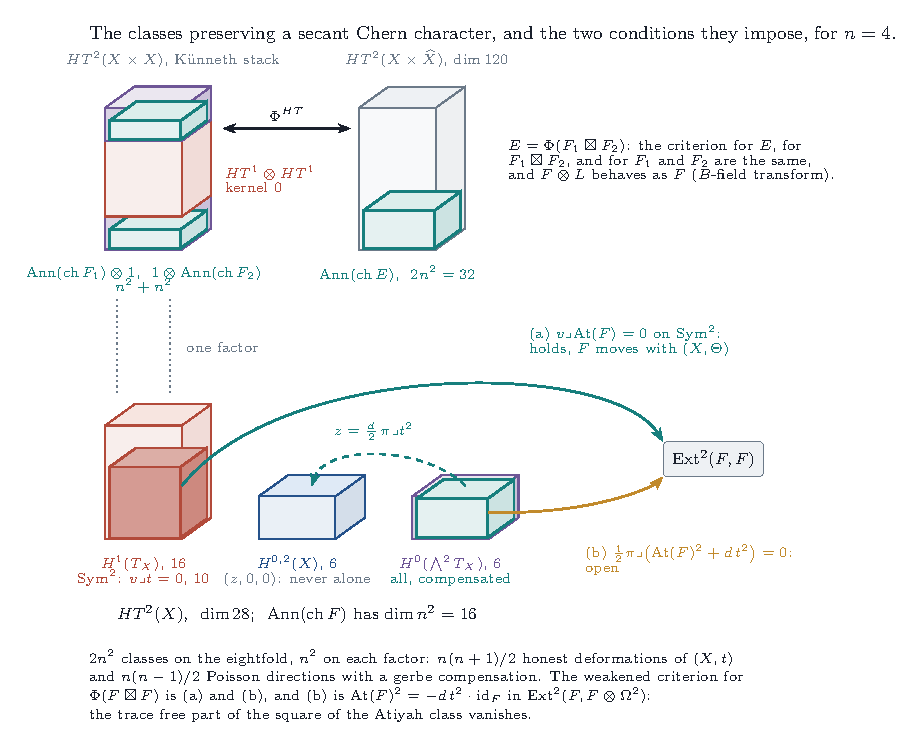
\includegraphics[width=\textwidth]{fig_factor}
\caption{\Cref{thm:factor} for $n=4$. Top: the K\"unneth stack of
$HT^{2}(X\times X)$, whose middle summand $HT^{1}\otimes HT^{1}$ meets the
kernel in zero by (i), so that the classes preserving $\ch(F_{1}\boxtimes F_{2})$
are two copies of the kernel on one factor; across Orlov's isomorphism,
$HT^{2}$ of the eightfold with the $2n^{2}$ classes preserving $\ch(E)$.
Bottom: $HT^{2}(X)$ as three slabs with heights proportional to their
dimensions, and inside them the $n^{2}$ classes of \eqref{eq:secantkernel}:
the polarised deformations in front of $H^{1}(T_{X})$, and the whole of
$H^{0}(\bigwedge^{2}T_{X})$, each bivector tilted into $H^{0,2}$ by its
compensation $\tfrac d2\,\pi\lrcorner t^{2}$; nothing in $H^{0,2}$ alone
preserves $\ch(F)$. On the right, the two conditions that the evaluation map
imposes on the two parts, (a) closed by the construction of $\cF$ and (b)
the identity \eqref{eq:heisenberg}.}
\label{fig:factor}
\end{figure}

\begin{corollary}[The one condition, on the fourfold]\label{cor:markmancondition}
In \Cref{setup:markman} let $E=\Phi(\cF\boxtimes\cF)$. Then $E$ satisfies the
weakened criterion of \cite[Question 11.4]{Mar25b} if and only if
\begin{equation}\label{eq:heisenberg}
  \mathrm{At}(\cF)^{2}=-d\,\Theta^{2}\cdot\id_{\cF}
  \qquad\text{in }\Ext^{2}(\cF,\cF\otimes\Omega^{2}_{X}).
\end{equation}
Equivalently, writing $\mathrm{At}(\cF)=\sum_{a}A_{a}\otimes p_{a}$ with
$A_{a}\in\Ext^{1}(\cF,\cF)$ in a basis $p_{a}$ of $H^{1,0}(X)$, all the
commutators $A_{a}A_{b}-A_{b}A_{a}\in\Ext^{2}(\cF,\cF)$ are the scalars
$\pm2d\,(q_{a}\wedge q_{b})\cdot\id_{\cF}$ prescribed by $\Theta^{2}$, the
sign being fixed by the Koszul rule.
\end{corollary}

\begin{proof}
By \Cref{prop:markman8}(iii), $\ch(\cF)=u_{\Theta}+3v_{\Theta}$, so
\Cref{thm:factor} applies with $n=4$, $(a,b)=(1,3)$ and $F_{1}=F_{2}=\cF$, and
$E$ satisfies the criterion if and only if $\cF$ satisfies (a) and (b). It
remains to see that (a) holds. The data of \Cref{setup:markman} are a
principally polarised fourfold $(X,\Theta)$ and $N$ points $x_{i}\in X$ with
$D_{i}=\tau_{x_{i}}^{*}\Theta$; the conditions imposed on the $D_{i}$, that
the intersections of two, three and four of them be smooth of the expected
codimension and that five of them be disjoint, are open in the parameter
space of such data over the local universal deformation $S$ of $(X,\Theta)$,
by the openness of smoothness for a proper flat family and the properness of
the projection; and the isolated points of $Z$, being transversal
intersections of four divisors, form a finite \'etale cover of the open set
where the conditions hold, so the $m$ points to be normalised can be followed
locally. The partial normalisation separates two smooth branches at each of
them and commutes with base change. So the construction produces a perfect
complex $\cF_{S}$ on the universal family over a neighbourhood of the base
point in $S$, whose fibre at the base point is $\cF$ and whose base has
Kodaira--Spencer image the whole space of polarised deformations, of
dimension $10=n(n+1)/2$. The obstruction $v\lrcorner\,\mathrm{At}(\cF)$ to
extending $\cF$ along $v$ vanishes for every $v$ along which $\cF$ does extend
\cite{Tod09}, which is (a).

For the reformulation, $\Omega^{1}_{X}=\cO_{X}\otimes H^{1,0}$ gives
$\mathrm{At}(\cF)=\sum_{a}A_{a}\otimes p_{a}$, and
$\mathrm{At}(\cF)^{2}=-\sum_{a<b}(A_{a}A_{b}-A_{b}A_{a})\otimes p_{a}\wedge p_{b}$
by the Koszul rule, while $\Theta^{2}=-2\sum_{a<b}(p_{a}\wedge p_{b})(q_{a}\wedge q_{b})$
for $\Theta=\sum_{a}p_{a}\wedge q_{a}$. Comparing coefficients of
$p_{a}\wedge p_{b}$ gives the commutator relations.
\end{proof}

\begin{remark}[What the reduction closes, and what it does not]\label{rem:factorclosed}
Three things are closed. First, the eightfold has disappeared: the condition
of \Cref{rem:onecondition}, on an object of rank $8d(d-9)$ on $X\times\widehat X$
of Weil type, is equivalent to one identity \eqref{eq:heisenberg} for a rank
one complex on the fourfold, in the Yoneda algebra $\Ext^{*}(\cF,\cF)$; the
dimension of the space of classes that has to be killed drops from $2n^{2}$
to $n^{2}$ and, by (a), to $n(n-1)/2=6$; at $n=3$ the count $n^{2}=9$ is the
nine-dimensional kernel of \cite[Corollaries 8.3.12 and 8.5.2]{Mar25a}, now
written out for every secant object in every dimension. Second, the half of that space made
of honest deformations imposes nothing, because Markman's construction is
uniform over the moduli of principally polarised fourfolds. Third, the two
forms of the criterion, for $E$ with $\ch(E)$ and for the twisted object with
$\kappa(E)$, are the same by \Cref{lem:bfield}, so nothing is lost by working
with the untwisted object.

The identity itself is a Heisenberg relation: the components of the Atiyah
class in the $n$ tangent directions must commute up to the scalars
prescribed by $\Theta^{2}$, and the only part of it that the Chern character
forces is the trace. It is exactly the statement that $\cF$ deforms, as an
object of the deformed category, along the Poisson directions of $X$
compensated by the gerbe classes $\tfrac d2\,\pi\lrcorner\,\Theta^{2}$, the
noncommutative first order deformations of $X$ with a gerby correction in
the language of \cite[Section 8.5]{Mar25a}. It holds
in the one case where the method is known to work: for Markman's sheaves
$\cF_{1}=I_{\bigcup C_{i}}(\Theta)$ on the Jacobian threefold of
\cite[Section 11.1]{Mar25b}, with $\ch=u_{\Theta}+v_{\Theta}$ and $d=q$, the
kernel of the obstruction map equals the annihilator of the Chern character
\cite[Corollary 8.3.12]{Mar25a}, which is stronger than the weakened
criterion, so by \Cref{thm:factor}(iii) these sheaves satisfy
$\mathrm{At}(\cF_{1})^{2}=-q\,\Theta^{2}\cdot\id$ on the threefold. For
the rank one complex of \Cref{setup:markman} on the fourfold the identity
is a computation of Yoneda products in $\Ext^{*}(\cF,\cF)$, and it can be
made local: the next paragraphs carry it out at one point of the support and
find that it fails.
\end{remark}

\subsubsection*{The identity fails at an isolated double point}

The identity \eqref{eq:heisenberg} can be tested locally. The evaluation map
is an algebra homomorphism \cite[(8.3.3)]{Mar25a}, so on a bivector
$\theta\wedge\theta'$ it is the Yoneda product of the classes
\[
  A_{\theta}=\operatorname{ev}_{\cF}(\theta)=\theta\lrcorner\,\mathrm{At}(\cF)
  \in\Ext^{1}(\cF,\cF),\qquad\theta\in H^{0}(T_{X}),
\]
which are the first order deformations of $\cF$ along the translations of
$X$; and the product of two global classes restricts to the product of their
germs. At a point where the support of $\cF$ has two smooth branches of
codimension two meeting transversally, the germs multiply nontrivially, and
since the compensating classes $z\cdot\id_{\cF}$ have zero germs, the
identity fails. Markman's construction has such points, and it cannot avoid
them.

\begin{lemma}[Localisation]\label{lem:edge}
Let $F$ be a perfect complex on a smooth projective variety $Y$, let
$\cE xt^{m}(F,F)$ be the sheaf associated with $U\mapsto\Hom_{D(U)}(F|_{U},F|_{U}[m])$,
and let $e\colon\Ext^{m}(F,F)\to H^{0}(Y,\cE xt^{m}(F,F))$ send a morphism
$F\to F[m]$ to its germs. Then $e$ is compatible with Yoneda products;
$e(z\cdot\id_{F})=0$ for $z\in H^{m}(\cO_{Y})$, $m\ge1$; and for
$\theta\in H^{0}(T_{Y})$ the germ of $A_{\theta}$ at $p$ is the class of the
jet extension $0\to F_{p}\to J_{\theta}(F_{p})\to F_{p}\to0$ of the germ
$F_{p}$ along the derivation $\theta$ of $\cO_{Y,p}$, which is
$\cO_{Y,p}$-linear in $\theta$.
\end{lemma}

\begin{proof}
Composition of morphisms commutes with restriction to open sets, which is the
first assertion. For the second, $z\cdot\id_{F}$ restricted to an affine open
$U$ is $z|_{U}\cdot\id_{F|_{U}}$, and $z|_{U}\in H^{m}(U,\cO_{U})=0$. For the
third, the Atiyah class of $F$ is the class of the first jet sequence
$0\to F\otimes\Omega^{1}_{Y}\to J^{1}(F)\to F\to0$ \cite[Section 3]{BF03},
its restriction to $U$ is the jet sequence of $F|_{U}$, and contracting with
$\theta$ is pushing out along $\id\otimes\theta\colon F\otimes\Omega^{1}\to F$,
which produces the extension $J_{\theta}(F)$ whose underlying sheaf is
$F\oplus F$ with $f\cdot(s,s')=(fs+\theta(f)s',fs')$. Linearity in $\theta$
is linearity of the contraction.
\end{proof}

\begin{lemma}[Two branches through a point]\label{lem:localproducts}
Let $\cO$ be the local ring of $\CC^{4}$ at the origin or its completion
$\CC[[x_{1},\dots,x_{4}]]$; let $P_{1}=\{x_{1}=x_{2}=0\}$ and
$P_{2}=\{x_{3}=x_{4}=0\}$, two smooth surfaces meeting transversally at the
origin; put $N_{1}=\langle\partial_{1},\partial_{2}\rangle$ and
$N_{2}=\langle\partial_{3},\partial_{4}\rangle$, the normal spaces of $P_{1}$
and of $P_{2}$ at the origin, so that
$\bigwedge^{2}T_{0}=\bigwedge^{2}N_{1}\oplus N_{1}\otimes N_{2}\oplus\bigwedge^{2}N_{2}$.
For a germ of vector field $\theta$ and a perfect complex $F$ of
$\cO$-modules write $a_{\theta}\in\Ext^{1}_{\cO}(F,F)$ for the class of the
jet extension along $\theta$.
\begin{enumerate}[label=\textup{(\roman*)},nosep]
\item For $F=I=I_{P_{1}}\cap I_{P_{2}}$, the ideal of the union,
  $\Ext^{2}_{\cO}(I,I)\cong N_{1}\otimes N_{2}$, a vector space of dimension
  four on which the maximal ideal acts trivially, and
  $a_{\theta}a_{\theta'}$ is, up to a fixed nonzero scalar, the component of
  $\theta(0)\wedge\theta'(0)$ in $N_{1}\otimes N_{2}$. In particular
  $a_{\theta}a_{\theta'}\ne0$ unless $\theta(0)\wedge\theta'(0)\in
  \bigwedge^{2}N_{1}\oplus\bigwedge^{2}N_{2}$.
\item For $F=K=[\cO\to\cO_{P_{1}}\oplus\cO_{P_{2}}]$, the complex in degrees
  $0$ and $1$ whose cohomology is $I$ in degree $0$ and the residue field $k$
  in degree $1$, $a_{\theta}a_{\theta'}\ne0$ unless
  $\theta(0)\wedge\theta'(0)\in N_{1}\otimes N_{2}$.
\end{enumerate}
In both cases the bilinear map $(\theta,\theta')\mapsto a_{\theta}a_{\theta'}$
is nonzero, and it depends only on $\theta(0)\wedge\theta'(0)$.
\end{lemma}

\begin{proof}
Write $A=\CC[x_{1},x_{2}]$, $B=\CC[x_{3},x_{4}]$, $R=A\otimes_{\CC}B$, with
maximal ideals $\mathfrak m_{A}$, $\mathfrak m_{B}$ at the origin, and
$k=\CC$. The ideal of the union is $I=\mathfrak m_{A}R\cap\mathfrak m_{B}R
=\mathfrak m_{A}\otimes_{\CC}\mathfrak m_{B}$, because the two ideals are
generated by disjoint sets of variables. Everything below is homogeneous, the
$\Ext$ groups in degree two are of finite length, and finite length modules
and jet classes are unchanged by the flat base change from $R$ to $\cO$; so we
compute over $R$. For finitely generated modules $M,M'$ over $A$ and $N,N'$
over $B$, the tensor product of free resolutions resolves $M\otimes_{\CC}N$
and the K\"unneth formula gives
\begin{equation}\label{eq:kunnethext}
  \Ext^{n}_{R}(M\otimes N,M'\otimes N')
  =\bigoplus_{i+j=n}\Ext^{i}_{A}(M,M')\otimes_{\CC}\Ext^{j}_{B}(N,N'),
\end{equation}
compatibly with Yoneda products up to the Koszul sign, since a product of
chain maps on the tensor product of resolutions is the tensor product of the
products.

The building block is one plane. The Koszul complex
$0\to A\xrightarrow{(-x_{2},x_{1})^{t}}A^{2}\xrightarrow{(x_{1},x_{2})}\mathfrak m_{A}\to0$
is a free resolution, so $\mathfrak m_{A}$ has projective dimension one and
$\Ext^{i}_{A}(\mathfrak m_{A},-)=0$ for $i\ge2$; and
$\Ext^{1}_{A}(\mathfrak m_{A},\mathfrak m_{A})=\coker\bigl(\Hom(A^{2},\mathfrak m_{A})
\to\Hom(A,\mathfrak m_{A})\bigr)=\mathfrak m_{A}/\mathfrak m_{A}^{2}$, a
two-dimensional space killed by $\mathfrak m_{A}$. On a complex of free
modules with differential $d$ the jet extension along a derivation $D$ is the
complex with terms $P_{i}\oplus P_{i}$ and differential
$\bigl(\begin{smallmatrix}d&-D(d)\\0&d\end{smallmatrix}\bigr)$, $D(d)$ the
entrywise derivative, because the twisted module $J_{D}(P_{i})$ is free on the
elements $(e,0)$ and $(0,e)$ and $d(0,e)=\sum_{l}d_{le}(0,e_{l})-\sum_{l}D(d_{le})(e_{l},0)$;
so the jet class is represented by the degree $-1$ chain map $-D(d)$. For
$D=\partial_{i}$ on the Koszul complex this is $e\mapsto\delta_{i2}f_{1}-\delta_{i1}f_{2}$
on the generator $e$ of the last term, whose image in
$\mathfrak m_{A}/\mathfrak m_{A}^{2}$ is $\delta_{i2}x_{1}-\delta_{i1}x_{2}$:
\[
  \alpha_{1}:=a_{\partial_{1}}=-[x_{2}],\qquad
  \alpha_{2}:=a_{\partial_{2}}=[x_{1}],
\]
a basis of $\Ext^{1}_{A}(\mathfrak m_{A},\mathfrak m_{A})$, which we identify
with $N_{1}$ by $\partial_{i}\mapsto\alpha_{i}$. Similarly $\beta_{3},\beta_{4}$
form a basis of $\Ext^{1}_{B}(\mathfrak m_{B},\mathfrak m_{B})$, identified
with $N_{2}$.

(i) By \eqref{eq:kunnethext} with $M=M'=\mathfrak m_{A}$, $N=N'=\mathfrak m_{B}$,
\[
  \Ext^{2}_{R}(I,I)=\Ext^{1}_{A}\otimes\Ext^{1}_{B}=N_{1}\otimes N_{2},
\]
the other two summands vanishing by the projective dimension, and it is killed
by $\mathfrak m_{A}$ and $\mathfrak m_{B}$. The derivation $\partial_{1}$ acts on
the factor $A$, so the jet extension of $I=\mathfrak m_{A}\otimes\mathfrak m_{B}$
along it is $J_{\partial_{1}}(\mathfrak m_{A})\otimes\mathfrak m_{B}$ and
$a_{\partial_{1}}=\alpha_{1}\otimes1$; likewise $a_{\partial_{2}}=\alpha_{2}\otimes1$,
$a_{\partial_{3}}=1\otimes\beta_{3}$, $a_{\partial_{4}}=1\otimes\beta_{4}$.
Hence $a_{\partial_{i}}a_{\partial_{j}}=\pm\alpha_{i}\otimes\beta_{j}$ for
$i\le2<j$, the four of them a basis of $N_{1}\otimes N_{2}$, while
$a_{\partial_{1}}a_{\partial_{2}}=\alpha_{1}\alpha_{2}\otimes1=0$ and
$a_{\partial_{3}}a_{\partial_{4}}=0$ because $\Ext^{2}_{A}(\mathfrak m_{A},\mathfrak m_{A})=0$.
For germs $\theta=\sum_{i}c^{i}\partial_{i}$ and $\theta'=\sum_{j}c'^{j}\partial_{j}$
the linearity of \Cref{lem:edge} and the triviality of the module structure
give $a_{\theta}a_{\theta'}=\sum_{i,j}c^{i}(0)c'^{j}(0)\,a_{\partial_{i}}a_{\partial_{j}}$,
the image of $\theta(0)\wedge\theta'(0)$ under the projection of
$\bigwedge^{2}T_{0}$ onto $N_{1}\otimes N_{2}$ followed by the isomorphism
$\partial_{i}\otimes\partial_{j}\mapsto\pm\alpha_{i}\otimes\beta_{j}$.

(ii) Let $Q=\cO_{P_{1}}\oplus\cO_{P_{2}}$. The map $\cO\to Q$ has kernel $I$
and cokernel $\cO/(I_{P_{1}}+I_{P_{2}})=k$, so $K$ sits in an exact triangle
$I\xrightarrow{\iota}K\xrightarrow{\pi}k[-1]\xrightarrow{\varepsilon}I[1]$.
The jet extension along $\theta$ is an exact functor, natural in its
argument, so the jet classes commute with $\iota$ and $\pi$; and for the
residue field $a^{k}_{\theta}$ depends only on $\theta(0)$, because
$\Ext^{1}(k,k)$ is killed by $\mathfrak m$ and the class is linear in
$\theta$. Therefore
\[
  \pi[2]\circ a^{K}_{\theta}a^{K}_{\theta'}
  =a^{k}_{\theta}a^{k}_{\theta'}\circ\pi
  =\pi^{*}\bigl(a^{k}_{\theta(0)}a^{k}_{\theta'(0)}\bigr),
  \qquad\pi^{*}\colon\Ext^{2}(k,k)\to\Ext^{1}(K,k),
\]
and it suffices to show that the right hand side is nonzero. The long exact
sequence of the triangle for $\Hom(-,k)$ reads
\[
  \Hom(I,k)\xrightarrow{\;\varepsilon^{*}\;}\Ext^{2}(k,k)\xrightarrow{\;\pi^{*}\;}
  \Ext^{1}(K,k),
\]
so $\ker\pi^{*}=\image\varepsilon^{*}$. Now $k=k_{A}\otimes k_{B}$ and, by
\eqref{eq:kunnethext}, $\Ext^{*}(k,k)$ is the tensor product of
$\Ext^{*}_{A}(k,k)$ and $\Ext^{*}_{B}(k,k)$. On the Koszul resolution
$A\to A^{2}\to A$ of $k_{A}$ the jet chain maps of $\partial_{1},\partial_{2}$
are $-D(d)$ as above, and their composite $A\to A$ is the scalar $-1$, whose
class in $\Ext^{2}_{A}(k,k)=\Hom(A,k)=k$ is nonzero; the degree one classes
$\gamma_{1},\gamma_{2}$ of $\partial_{1},\partial_{2}$ are the basis
$-e_{1}^{*},-e_{2}^{*}$ of $\Ext^{1}_{A}(k,k)=\Hom(A^{2},k)$, and their
product spans $\Ext^{2}_{A}(k,k)$. With the analogous classes
$\gamma_{3},\gamma_{4}$ over $B$, the products $\gamma_{1}\gamma_{2}\otimes1$,
$\gamma_{i}\otimes\gamma_{j}$ ($i\le2<j$) and $1\otimes\gamma_{3}\gamma_{4}$
form a basis of $\Ext^{2}(k,k)=k\oplus(k^{2}\otimes k^{2})\oplus k$, so
$\partial_{i}\wedge\partial_{j}\mapsto a^{k}_{\partial_{i}}a^{k}_{\partial_{j}}$
identifies $\bigwedge^{2}(N_{1}\oplus N_{2})$ with $\Ext^{2}(k,k)$, and
$a^{k}_{\theta(0)}a^{k}_{\theta'(0)}$ is the image of $\theta(0)\wedge\theta'(0)$. The
class $\varepsilon$ is the K\"unneth product $\varepsilon_{A}\otimes\varepsilon_{B}$
of the classes of $0\to\mathfrak m_{A}\to A\to k\to0$ and its $B$-analogue,
because $K$ is the two-step truncation of the tensor product of the complexes
$[A\to k_{A}]$ and $[B\to k_{B}]$ and $\varepsilon$ is the inclusion of the
omitted term $k_{A}\otimes k_{B}$. Hence $\varepsilon^{*}$ maps
$\Hom(I,k)=\Hom(\mathfrak m_{A},k)\otimes\Hom(\mathfrak m_{B},k)$ into
$\Ext^{1}_{A}(k,k)\otimes\Ext^{1}_{B}(k,k)=N_{1}\otimes N_{2}$, and onto it,
since $\Hom(\mathfrak m_{A},k)\to\Ext^{1}_{A}(k,k)$ is an isomorphism: it is
the connecting homomorphism of the sequence, injective because
$\Hom(A,k)\to\Hom(\mathfrak m_{A},k)$ is zero and surjective because
$\Ext^{1}_{A}(A,k)=0$. So $\ker\pi^{*}=N_{1}\otimes N_{2}$
and $\pi^{*}(\theta(0)\wedge\theta'(0))\ne0$ exactly when
$\theta(0)\wedge\theta'(0)\notin N_{1}\otimes N_{2}$.

Both computations are repeated by machine in item (XXIX) of
\Cref{sec:verification}, which also finds $\Ext^{2}_{\cO}(K,K)\cong
\bigwedge^{2}N_{1}\oplus\bigwedge^{2}N_{2}$ with $a_{\theta}a_{\theta'}$ the
projection of $\theta(0)\wedge\theta'(0)$ to it, the exact complement of (i).
\end{proof}

\begin{theorem}[Markman's candidate does not satisfy the weakened criterion]
\label{thm:candidatefails}
In \Cref{setup:markman}, for every odd $d\ge3$, every choice of the
translates $D_{i}$ in general position and every choice of the $m$ points to
be normalised:
\begin{enumerate}[label=\textup{(\roman*)},nosep]
\item the identity \eqref{eq:heisenberg} fails: there is a constant bivector
  $\pi\in H^{0}(\bigwedge^{2}T_{X})$ with
  $\tfrac12\pi\lrcorner\bigl(\mathrm{At}(\cF)^{2}+d\,\Theta^{2}\cdot\id_{\cF}\bigr)\ne0$
  in $\Ext^{2}(\cF,\cF)$;
\item $\cF$ does not satisfy the weakened criterion: the class
  $x_{\cF}=(\tfrac d2\,\pi\lrcorner\,\Theta^{2},0,\pi)$ has
  $x_{\cF}\lrcorner\,\ch(\cF)=0$ and $\operatorname{ev}_{\cF}(x_{\cF})\ne0$;
\item for every perfect complex $F_{2}$ on $X$ with Chern character on the
  secant plane, in particular for $F_{2}=\cF$ and $F_{2}=\cF^{\vee}$, the
  object $E=\Phi(\cF\boxtimes F_{2})$ on the eightfold $X\times\widehat X$ of
  Weil type does not satisfy the weakened criterion of
  \cite[Question 11.4]{Mar25b}: the class $x=\Phi^{HT}(x_{\cF}\otimes1)$
  satisfies $x\lrcorner\,\ch(E)=0$ and $\operatorname{ev}_{E}(x)\ne0$, so
  $\sigma_{E}$ is not injective on the image of $\operatorname{ev}_{E}$.
\end{enumerate}
\end{theorem}

\begin{proof}
(i) The surfaces $Z_{i}$ and $Z_{j}$ at cyclic distance at least three meet
in the $24$ points of $D_{i}\cap D_{i+1}\cap D_{j}\cap D_{j+1}$, and there are
$12N(N-5)=(d+9)(3d-3)$ such points, of which $m=(d+9)(2d-1)$ are normalised;
the remaining $(d+9)(d-2)\ge12$ are not. Let $p$ be one of them. The four
divisors through $p$ meet transversally, so their local equations
$x_{1},\dots,x_{4}$ form a regular system of parameters of $\cO_{X,p}$ and
identify its completion with $\CC[[x_{1},\dots,x_{4}]]$, with
$D_{i}=\{x_{1}=0\}$, $D_{i+1}=\{x_{2}=0\}$, $D_{j}=\{x_{3}=0\}$,
$D_{j+1}=\{x_{4}=0\}$, hence $Z_{i}=P_{1}$ and $Z_{j}=P_{2}$ in the
notation of \Cref{lem:localproducts}; the completion is flat, so a class
whose completed germ is nonzero is nonzero. No other
$D_{k}$ passes through $p$, five divisors having empty intersection, so no
other component of $Z$ does. Near $p$ the map $\nu$ is an isomorphism,
$\nu_{*}\cO_{\widetilde Z}=\cO_{Z}$, and $\cF$ is the ideal sheaf
$I_{Z}=I_{P_{1}}\cap I_{P_{2}}$ twisted by the locally trivial $\cO_{X}(3\Theta)$:
the germ $\cF_{p}$ is the module $I$ of \Cref{lem:localproducts}(i).

Let $\theta,\theta'\in H^{0}(T_{X})$ be constant vector fields whose values
at $p$ are $\partial_{1}$ and $\partial_{3}$; they exist because the constant
fields span every tangent space. Put $\pi=\theta\wedge\theta'$. Since
$\operatorname{ev}_{\cF}$ is an algebra homomorphism,
$\operatorname{ev}_{\cF}(\pi)=\tfrac12\pi\lrcorner\,\mathrm{At}(\cF)^{2}
=A_{\theta}A_{\theta'}$, and by \Cref{lem:edge} its germ at $p$ is
$a_{\theta}a_{\theta'}$, which is nonzero by \Cref{lem:localproducts}(i),
$\partial_{1}\wedge\partial_{3}$ having nonzero component in $N_{1}\otimes N_{2}$.
The germ of $\tfrac d2(\pi\lrcorner\,\Theta^{2})\cdot\id_{\cF}$ at $p$ is zero
by the same lemma. So the germ at $p$ of
$\tfrac12\pi\lrcorner(\mathrm{At}(\cF)^{2}+d\Theta^{2}\cdot\id_{\cF})$ is
$a_{\theta}a_{\theta'}\ne0$, and the class itself is nonzero.

(ii) By \Cref{thm:factor}(ii) the class $x_{\cF}$ preserves $\ch(\cF)$, and by
\eqref{eq:evgeneral} $\operatorname{ev}_{\cF}(x_{\cF})$ is the class of (i).

(iii) $\ch(\cF^{\vee})=u_{\Theta}-3v_{\Theta}$ lies on the secant plane. By
\Cref{thm:factor}(iv), $E$ satisfies the criterion only if both factors do,
and $\cF$ does not; the displayed class is the transport of
$x_{\cF}\otimes1\in\Ann_{HT^{2}}(\ch(\cF\boxtimes F_{2}))$, on which
$\operatorname{ev}$ is $\pm\operatorname{ev}_{\cF}(x_{\cF})\otimes\id_{F_{2}}\ne0$.
The last assertion is \Cref{setup:criterion}:
$\sigma_{E}(\operatorname{ev}_{E}(x))=x\lrcorner\,\ch(E)=0$ with
$\operatorname{ev}_{E}(x)\ne0$.
\end{proof}

\begin{remark}[The normalised points obstruct as well]\label{rem:normalisedpoints}
At a normalised point the germ of $\cF$ is the complex $K$ of
\Cref{lem:localproducts}(ii), and the same argument with $\theta(p)=\partial_{1}$,
$\theta'(p)=\partial_{2}$ produces a nonzero germ. So the failure does not
depend on which points are separated, and separating all of them would not
help even if it were allowed: normalising every isolated point changes
$\chi(\cO_{\widetilde Z})$ to $110N-12N^{2}+12N(N-5)=50N$, while the secant
plane requires $(d+9)(27-d)=72N-4N^{2}$, and the two agree only for
$N=11/2$. The two local computations are complementary: at a point of type
(i) the obstruction lives in $N_{1}\otimes N_{2}$, at a point of type (ii) in
$\bigwedge^{2}N_{1}\oplus\bigwedge^{2}N_{2}$, and together they exhaust
$\bigwedge^{2}T_{p}$.
\end{remark}

\begin{figure}[tbp]
\centering
  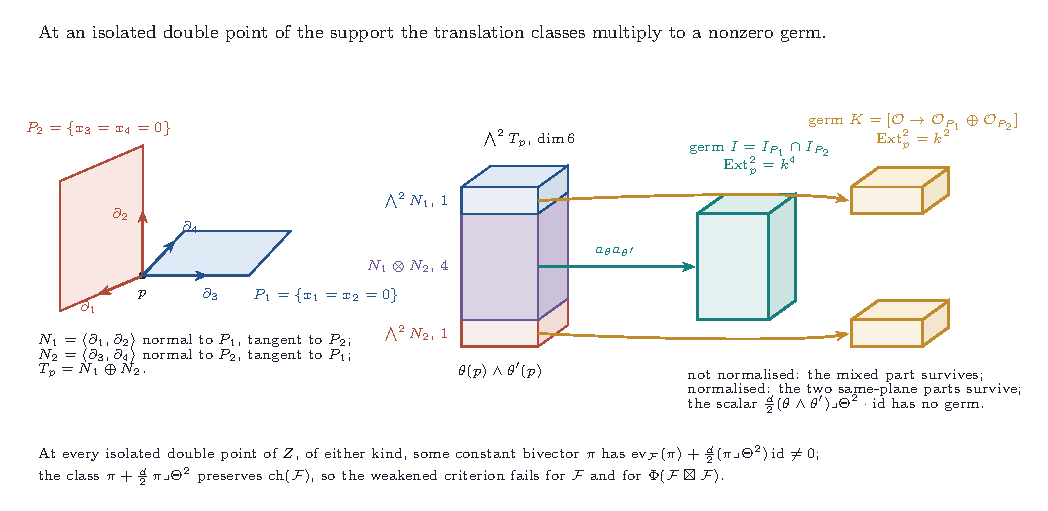
\includegraphics[width=\textwidth]{fig_doublepoint}
\caption{\Cref{lem:localproducts} and \Cref{thm:candidatefails}. Left: two
smooth surfaces of a fourfold meeting transversally at $p$, with the normal
spaces $N_{1}$ and $N_{2}$, each tangent to the other branch. Centre: the
bivectors at $p$, split into $\bigwedge^{2}N_{1}$, $N_{1}\otimes N_{2}$ and
$\bigwedge^{2}N_{2}$, with heights proportional to the dimensions. Right: the
local $\Ext^{2}$ of the germ of $\cF$ at $p$ in the two cases, and the part
of the bivectors that the products of the translation classes carry onto it:
the mixed part when the point is not normalised, the two same-plane parts
when it is. The compensating scalar has no germ, so in either case the
identity \eqref{eq:heisenberg} fails at $p$.}
\label{fig:doublepoint}
\end{figure}

\begin{corollary}[A local obstruction in every dimension]\label{cor:localobstruction}
Let $(X,t)$ be a polarised abelian variety of dimension $n\ge4$ and $F$ a
perfect complex on $X$ with $\ch(F)=au_{t}+bv_{t}$, $(a,b)\ne(0,0)$. Suppose
that at some point $p$ the germ $F_{p}$ is isomorphic, in the derived
category of $\cO_{X,p}$-modules, to the ideal of the union of two smooth germs
of codimension two meeting transversally along a germ of codimension four,
or, when $n=4$, to the complex $[\cO\to\cO_{P_{1}}\oplus\cO_{P_{2}}]$ of two
such germs. Then $F$ does not satisfy the weakened criterion, and neither does
$\Phi(F\boxtimes F_{2})$ on $X\times\widehat X$ for any secant $F_{2}$. In
particular, in every dimension $n\ge4$, the union $Z$ of the intersections
$D_{i}\cap D_{i+1}$ of consecutive translates of a polarisation in general
position contains, for every pair $(i,j)$ of nonconsecutive indices, a
subvariety $Z_{i}\cap Z_{j}$ of codimension four along which $Z$ has two
transversal branches; any secant object of the form $[\cO_{X}\to\nu_{*}\cO_{\widetilde Z}]\otimes L$
in which $\nu$ is an isomorphism at a general point of one such
$Z_{i}\cap Z_{j}$ fails the criterion.
\end{corollary}

\begin{proof}
In formal coordinates $x_{1},\dots,x_{n}$ at $p$ with the two branches
$\{x_{1}=x_{2}=0\}$ and $\{x_{3}=x_{4}=0\}$, which exist because the four
local equations of the branches form part of a regular system of
parameters, the ideal is
$I\otimes_{\CC}\CC[x_{5},\dots,x_{n}]$ with $I$ as in \Cref{lem:localproducts},
and \eqref{eq:kunnethext} with the third factor gives
$\Ext^{2}(I_{p},I_{p})=N_{1}\otimes N_{2}\otimes\cO_{W,p}$, $W$ the
intersection of the branches. The jet classes along $\partial_{5},\dots,\partial_{n}$
vanish, these derivations acting on a free factor, and the products of the
classes along $\partial_{1},\dots,\partial_{4}$ are as in the lemma; reducing
modulo the maximal ideal of $\cO_{W,p}$ shows that $a_{\theta}a_{\theta'}\ne0$
whenever $\theta(p)\wedge\theta'(p)$ has a nonzero component in
$N_{1}\otimes N_{2}$. The rest of the argument is that of
\Cref{thm:candidatefails}, using \Cref{thm:factor} for $n\ge3$. For the last
assertion, $Z_{i}\cap Z_{j}=D_{i}\cap D_{i+1}\cap D_{j}\cap D_{j+1}$ is a
transversal intersection of four divisors, of codimension four, and at a
general point of it no fifth divisor passes, so $Z$ has exactly the two
branches $Z_{i}$ and $Z_{j}$ there.
\end{proof}

\begin{remark}[What this settles]\label{rem:candidatemeaning}
\Cref{thm:candidatefails} answers the question left open in
\cite[Section 12]{Mar25b}: the secant objects proposed there do not satisfy
the weaker criterion of Question 11.4, for any discriminant. The reason is
local and geometric. Question 11.4 asks whether the semiregularity map may be
required to be injective only on the image of the evaluation map; for a
secant object that image contains, by \Cref{thm:factor}, the products
$A_{\theta}A_{\theta'}$ of the translation classes shifted by the scalars
$\tfrac d2(\theta\wedge\theta')\lrcorner\,\Theta^{2}$, and the semiregularity
map kills them all. For the criterion to hold these shifted products must
vanish, and they cannot: at an isolated double point of the support, the
translation classes of the two branches multiply to a nonzero local class,
while a scalar has no local class at all. What survives of the fourth
ingredient of \Cref{rem:deformation} is therefore sharper than before. A
secant object of positive rank on a fourfold that satisfies the weakened
criterion must have, at every point, germs whose translation classes multiply
to zero in the local $\Ext^{2}$; by \Cref{lem:localproducts} this excludes
every support with two transversal branches of codimension two through a
point, whether or not the branches are separated, and by
\Cref{cor:localobstruction} it excludes the chain of consecutive
intersections of translates in every dimension. An object supported on a
smooth surface, or on surfaces meeting only along curves, is not excluded by
this argument, but no such object with Chern character on the secant plane
is known.
\end{remark}

\subsection{Smooth support, and the four discriminants}
\label{ssec:smoothsupport}

\Cref{thm:candidatefails} and \Cref{cor:localobstruction} remove every secant
object whose support carries two transversal branches of codimension two
through a point. What they leave is a support that is smooth, or that meets
itself only along curves, and \Cref{rem:candidatemeaning} closes with the
remark that no such object is known. This subsection says why the local
argument cannot reach that case, and then determines what the case can be.
The answer is narrow: on the fourfold the invariants of the support are
forced outright, and the discriminant is confined to a finite list.

The first point is that at a smooth point there is nothing local left to
compute.

\begin{proposition}[No local obstruction at a smooth point]\label{prop:smoothlocal}
Let $Y$ be a smooth variety with $\omega_{Y}\cong\cO_{Y}$ and let $S\subset Y$
be smooth of codimension two. Then
\[
  \cE xt^{0}(\cI_{S},\cI_{S})=\cO_{Y},\qquad
  \cE xt^{1}(\cI_{S},\cI_{S})=N_{S/Y},\qquad
  \cE xt^{q}(\cI_{S},\cI_{S})=0\quad(q\ge2),
\]
and the same holds for $\cI_{S}\otimes L$ for any line bundle $L$.
Consequently, for $F=\cI_{S}\otimes L$ both sides of \eqref{eq:heisenberg}
have vanishing germs in $\cE xt^{2}$, and \Cref{lem:edge} decides nothing.
\end{proposition}

\begin{proof}
Twisting by $L$ changes neither side, so take $F=\cI_{S}$. The sheaf
$\cI_{S}$ is torsion free of rank one and reflexive, whence
$\cE xt^{0}(\cI_{S},\cI_{S})=\cO_{Y}$. Apply $\cH om(-,\cI_{S})$ to
\begin{equation}\label{eq:idealseq}
  0\to\cI_{S}\to\cO_{Y}\to\cO_{S}\to0 .
\end{equation}
Since $\cE xt^{q}(\cO_{Y},\cI_{S})=0$ for $q\ge1$, the long exact sequence
gives
\begin{equation}\label{eq:shift}
  \cE xt^{q}(\cI_{S},\cI_{S})\cong\cE xt^{q+1}(\cO_{S},\cI_{S})
  \qquad(q\ge1).
\end{equation}
Now apply $\cH om(\cO_{S},-)$ to \eqref{eq:idealseq}. Because $S$ is smooth of
codimension two, hence a local complete intersection, the Koszul resolution
gives $\cE xt^{k}(\cO_{S},\cO_{Y})=0$ for $k\ne2$ and
$\cE xt^{2}(\cO_{S},\cO_{Y})=\omega_{S}\otimes\omega_{Y}^{-1}=\omega_{S}$,
while $\cE xt^{k}(\cO_{S},\cO_{S})=\bigwedge^{k}N_{S/Y}$ for $0\le k\le2$ and
zero otherwise. Computing both from the same Koszul complex shows that the
map
\[
  \rho\colon\cE xt^{2}(\cO_{S},\cO_{Y})=\omega_{S}
  \longrightarrow
  \cE xt^{2}(\cO_{S},\cO_{S})=\textstyle\bigwedge^{2}N_{S/Y}=\omega_{S}
\]
induced by $\cO_{Y}\to\cO_{S}$ is the identity: in local coordinates in which
$S=\{x_{1}=x_{2}=0\}$, both groups are computed as $M/(x_{1},x_{2})M$ for
$M=\cO_{Y}$ and $M=\cO_{S}$, and the map is reduction modulo $(x_{1},x_{2})$,
which is the identity on $\cO_{S}$.

Take $k=2$ in the long exact sequence of $\cH om(\cO_{S},-)$. Since $\rho$ is
surjective and $\cE xt^{3}(\cO_{S},\cO_{Y})=0$, the segment
\[
  \cE xt^{2}(\cO_{S},\cO_{Y})\xrightarrow{\ \rho\ }
  \cE xt^{2}(\cO_{S},\cO_{S})\to
  \cE xt^{3}(\cO_{S},\cI_{S})\to
  \cE xt^{3}(\cO_{S},\cO_{Y})=0
\]
gives $\cE xt^{3}(\cO_{S},\cI_{S})=0$, so $\cE xt^{2}(\cI_{S},\cI_{S})=0$ by
\eqref{eq:shift}. For $k\ge3$ both $\cE xt^{k}(\cO_{S},\cO_{Y})$ and
$\cE xt^{k}(\cO_{S},\cO_{S})$ vanish, so
$\cE xt^{k+1}(\cO_{S},\cI_{S})=0$ and $\cE xt^{k}(\cI_{S},\cI_{S})=0$. Taking
$k=1$ and using that $\rho$ is injective, the segment
\[
  0=\cE xt^{1}(\cO_{S},\cO_{Y})\to
  \cE xt^{1}(\cO_{S},\cO_{S})=N_{S/Y}\to
  \cE xt^{2}(\cO_{S},\cI_{S})\to
  \cE xt^{2}(\cO_{S},\cO_{Y})\xrightarrow{\ \rho\ }
\]
exhibits $\cE xt^{2}(\cO_{S},\cI_{S})\cong N_{S/Y}$, which is
$\cE xt^{1}(\cI_{S},\cI_{S})$ by \eqref{eq:shift}.

For the last assertion, the right side of \eqref{eq:heisenberg} has vanishing
germs by \Cref{lem:edge}, and the left side lies in
$\Ext^{2}(F,F\otimes\Omega^{2}_{Y})$ whose sheaf of germs in the
$\cE xt^{2}$ direction is $\cE xt^{2}(F,F)\otimes\Omega^{2}_{Y}=0$.
\end{proof}

\begin{remark}[Where the obstruction goes instead]\label{rem:obstructionmoves}
\Cref{prop:smoothlocal} is the precise reason the argument of
\Cref{thm:candidatefails} stops at a smooth support, and it also says what
replaces it. With $\cE xt^{2}=0$ the local to global spectral sequence for
$\Ext^{2}(\cI_{S},\cI_{S})$ has only two surviving rows, $H^{1}(S,N_{S/Y})$
and $H^{2}(Y,\cO_{Y})$, and they sit in different steps of the filtration: the
first is the quotient that records the geometry of $S$, the second the
subgroup of scalars. A product $A_{\theta}A_{\theta'}$ of translation classes
therefore has a well defined image in $H^{1}(S,N_{S/Y})$, while the scalar on
the right of \eqref{eq:heisenberg} has image zero there. So the criterion
splits into two conditions of different kinds: a vanishing in
$H^{1}(S,N_{S/Y})$, which is a statement about the normal bundle and not about
any point, and an identity in $H^{2}(Y,\cO_{Y})$. At a double point the first
of these was already inconsistent locally. At a smooth support it is a global
question, and we do not decide it. What we can decide is which $S$ are even
available.
\end{remark}

The invariants of a smooth support are not free. On an abelian variety the
Todd class is trivial, so Grothendieck--Riemann--Roch turns the Chern
character of the object into the complete numerical package of the surface,
and three classical inequalities then close in on it.

\begin{theorem}[The invariants of a smooth support]\label{thm:smoothinvariants}
Let $(X,\Theta)$ be a principally polarised abelian fourfold, let $d>0$, let
$b\in\ZZ_{>0}$, and let $\cF=\cI_{S}(b\Theta)$ be a coherent sheaf with
\[
  \ch(\cF)=u_{\Theta}+b\,v_{\Theta}
\]
and $S\subset X$ smooth. Write $N=\tfrac12\Nm_{K/\QQ}(b+\sqrt{-d})
=\tfrac12(b^{2}+d)$, $\iota\colon S\hookrightarrow X$ and
$\lambda=\iota^{*}\Theta$. Then $S$ is a surface and
\begin{equation}\label{eq:smoothinvariants}
\begin{aligned}
  [S]&=N\Theta^{2}, &\qquad \iota_{*}K_{S}&=\tfrac{4bN}{3}\,\Theta^{3},
  &\qquad \chi(\cO_{S})&=4N(2b^{2}-N),\\
  K_{S}^{2}&=12N(4b^{2}-N), &\qquad e(S)&=12N(4b^{2}-3N),
  &\qquad K_{S}\cdot\lambda&=32bN,
\end{aligned}
\end{equation}
with $\lambda^{2}=24N$ and $[S]^{2}=24N^{2}$. Moreover $K_{S}$ is globally
generated, hence nef; $S$ is minimal of general type; and
\begin{equation}\label{eq:threebounds}
  \tfrac{4}{9}b^{2}\ \le\ N\ \le\ b^{2},
  \qquad\text{equivalently}\qquad
  -\tfrac{1}{9}b^{2}\ \le\ d\ \le\ b^{2} .
\end{equation}
The lower bound is the Hodge index theorem and is implied by $d>0$; the upper
bound is the Bogomolov--Miyaoka--Yau inequality. In terms of $b$ and $d$ the
five invariants read
\begin{equation}\label{eq:bdform}
  \chi(\cO_{S})=(b^{2}+d)(3b^{2}-d),\quad
  K_{S}^{2}=3(b^{2}+d)(7b^{2}-d),\quad
  e(S)=3(b^{2}+d)(5b^{2}-3d),
\end{equation}
and the defect in the Bogomolov--Miyaoka--Yau inequality is
\begin{equation}\label{eq:bmydefect}
  3e(S)-K_{S}^{2}=24\,(b^{4}-d^{2}),
\end{equation}
so that the inequality is exactly $d\le b^{2}$ and nothing else.
Finally $K_{S}$ is never numerically proportional to $\lambda$.
\end{theorem}

\begin{proof}
Since $\ch_{0}(\cF)=1$ and $c_{1}(\cF)=b\Theta$, the sheaf
$\cF(-b\Theta)=\cI_{S}$ has $\ch_{0}=1$, $\ch_{1}=0$, so $S$ has codimension
at least two, and
\[
  \ch(\cO_{S})=1-\ch(\cI_{S})=1-\ch(\cF)\,e^{-b\Theta}.
\]
Expanding the right side in $\QQ[\Theta]/(\Theta^{5})$ and collecting gives
\[
  \ch_{2}(\cO_{S})=\tfrac{b^{2}+d}{2}\Theta^{2}=N\Theta^{2},\quad
  \ch_{3}(\cO_{S})=-\tfrac{2bN}{3}\Theta^{3},\quad
  \ch_{4}(\cO_{S})=\tfrac{3b^{4}+2db^{2}-d^{2}}{24}\Theta^{4},
\]
which is the computation of item (XXX) of \Cref{sec:verification}. The first
identity says $S$ has codimension exactly two, so it is a surface, with class
$N\Theta^{2}$. Because $T_{X}$ is trivial, $\td(T_{X})=1$, and
Grothendieck--Riemann--Roch for $\iota$ reads
$\ch(\iota_{*}\cO_{S})=\iota_{*}\td(T_{S})$. Comparing degrees three and four,
\[
  \ch_{3}(\cO_{S})=\iota_{*}\tfrac{c_{1}(T_{S})}{2}=-\tfrac12\iota_{*}K_{S},
  \qquad
  \ch_{4}(\cO_{S})=\iota_{*}\tfrac{c_{1}^{2}+c_{2}}{12}
  =\chi(\cO_{S})\,[\mathrm{pt}],
\]
the second by Noether's formula. With $\Theta^{4}=24\,[\mathrm{pt}]$ these give
$\iota_{*}K_{S}=\tfrac{4bN}{3}\Theta^{3}$ and, after substituting
$d=2N-b^{2}$, $\chi(\cO_{S})=3b^{4}+2db^{2}-d^{2}=4N(2b^{2}-N)$.
Then $K_{S}\cdot\lambda=\int_{X}\iota_{*}K_{S}\cdot\Theta=\tfrac{4bN}{3}\cdot24=32bN$
and $\lambda^{2}=\int_{X}[S]\cdot\Theta^{2}=24N$.

For the last two invariants, the normal bundle sequence and the triviality of
$T_{X}$ give $c(T_{S})c(N_{S/X})=1$, so $c_{1}(N_{S/X})=K_{S}$ and
$c_{2}(N_{S/X})=K_{S}^{2}-e(S)$; the self-intersection formula
$[S]^{2}=\int_{S}c_{2}(N_{S/X})$ then reads
\[
  24N^{2}=K_{S}^{2}-e(S),
\]
while Noether's formula reads $12\chi(\cO_{S})=K_{S}^{2}+e(S)$. Solving the
two gives the stated $K_{S}^{2}$ and $e(S)$.

The conormal sequence presents $\Omega^{1}_{S}$ as a quotient of
$\Omega^{1}_{X}|_{S}=\cO_{S}^{\oplus4}$, so $\Omega^{1}_{S}$ is globally
generated, and therefore so is $K_{S}=\det\Omega^{1}_{S}$, a quotient of
$\bigwedge^{2}\cO_{S}^{\oplus4}$. A globally generated line bundle is nef. A
globally generated rank two bundle on a surface has $c_{2}\ge0$, the class
$c_{2}$ being represented by the vanishing scheme of a general section, which
is empty or finite; hence
\[
  e(S)=c_{2}(\Omega^{1}_{S})=12N(4b^{2}-3N)\ \ge\ 0,
\]
so $N\le\tfrac43b^{2}<4b^{2}$ and therefore $K_{S}^{2}=12N(4b^{2}-N)>0$. A nef
divisor of positive self-intersection is big, so $\kappa(S)=2$ and, $K_{S}$
being nef, $S$ is minimal of general type. The Bogomolov--Miyaoka--Yau
inequality $c_{1}^{2}\le3c_{2}$ then applies and reads
$K_{S}^{2}\le3e(S)$. Substituting $N=\tfrac12(b^{2}+d)$ in the two
expressions gives \eqref{eq:bdform}, hence
$3e(S)-K_{S}^{2}=24(b^{4}-d^{2})$, and the inequality is $d\le b^{2}$, that
is $N\le b^{2}$.

For the lower bound, $\lambda$ is ample on $S$, so the Hodge index theorem
gives $(K_{S}\cdot\lambda)^{2}\ge K_{S}^{2}\,\lambda^{2}$, that is
$(32bN)^{2}\ge12N(4b^{2}-N)\cdot24N$, which simplifies to $9N\ge4b^{2}$. Since
$N=\tfrac12(b^{2}+d)$ with $d>0$, this holds automatically. Equality in the
Hodge index theorem occurs exactly when $K_{S}$ is numerically proportional to
$\lambda$, hence exactly when $9N=4b^{2}$; as $9N=\tfrac92(b^{2}+d)>4b^{2}$ for
$d>0$, that never happens.
\end{proof}

\begin{corollary}[Four discriminants on the fourfold]\label{cor:fourdiscriminants}
In \Cref{setup:markman}, where $b=3$ by \Cref{prop:markman8}(iii), a secant
object $\cI_{S}(3\Theta)$ with smooth support exists only if $d\le9$; since
$d$ is squarefree this leaves $d\in\{1,2,3,5,6,7\}$, and if in addition
$N=(9+d)/2$ is an integer, which is what a support assembled from translates
of $\Theta$ requires, only
\[
  d\in\{1,\,3,\,5,\,7\},\qquad N\in\{5,\,6,\,7,\,8\}.
\]
For these the invariants are forced to the values in
\Cref{tab:smoothsupport}. In particular, for every imaginary quadratic field
of discriminant larger than $9$ there is no secant object of rank one with
smooth support on an abelian fourfold at all.
\end{corollary}

\begin{proof}
Immediate from \eqref{eq:threebounds} at $b=3$, together with the arithmetic
of \eqref{eq:smoothinvariants}; the table is item (XXX) of
\Cref{sec:verification}. The value $d=9$ is the equality case of
Bogomolov--Miyaoka--Yau, where $K_{S}^{2}=3e(S)=2916$ and $S$ would have to be
a quotient of the ball; it is excluded here because $9$ is not squarefree.
\end{proof}

\begin{table}[htbp]
\centering
\small
\renewcommand{\arraystretch}{1.12}
\begin{tabular}{@{}ccrrrrr@{}}
\toprule
$d$ & $N$ & $\chi(\cO_{S})$ & $K_{S}^{2}$ & $e(S)$ &
$K_{S}\cdot\lambda$ & $\lambda^{2}$ \\
\midrule
$1$ & $5$ & $260$ & $1860$ & $1260$ & $480$ & $120$ \\
$3$ & $6$ & $288$ & $2160$ & $1296$ & $576$ & $144$ \\
$5$ & $7$ & $308$ & $2436$ & $1260$ & $672$ & $168$ \\
$7$ & $8$ & $320$ & $2688$ & $1152$ & $768$ & $192$ \\
\bottomrule
\end{tabular}
\caption{The only invariants a smooth support can have on an abelian
fourfold, by \Cref{thm:smoothinvariants} and
\Cref{cor:fourdiscriminants}, at $b=3$ and with $N$ an integer. Every entry is
forced by $\ch(\cF)$ alone; none is a choice. The slope
$K_{S}^{2}/\chi(\cO_{S})$ runs from $93/13$ at $d=1$ to $42/5$ at $d=7$, and
reaches the Bogomolov--Miyaoka--Yau ceiling of $9$ only at the excluded value
$d=9$.}
\label{tab:smoothsupport}
\end{table}

\begin{figure}[htbp]
\centering
  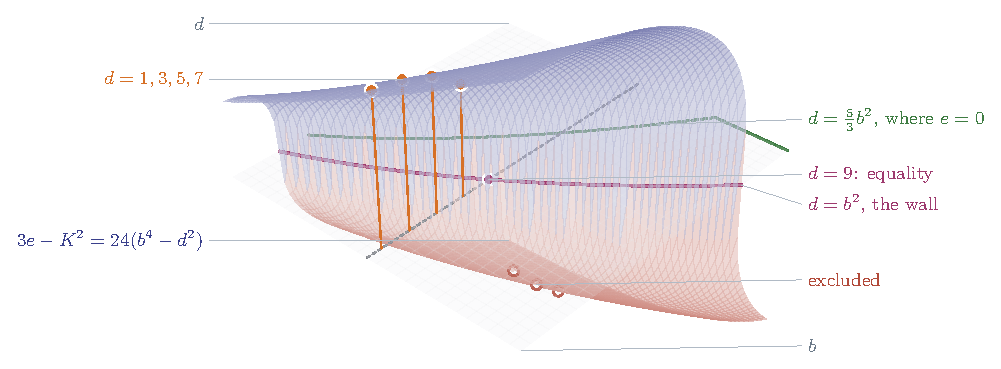
\includegraphics[width=\textwidth]{fig_bmywindow}
\caption{\Cref{thm:smoothinvariants} over the quarter plane of $(b,d)$. The
height of the surface is the defect $3e(S)-K_{S}^{2}=24(b^{4}-d^{2})$ in the
Bogomolov--Miyaoka--Yau inequality for the surface the theorem attaches to the
pair, compressed by a signed cube root so that four orders of magnitude fit
one frame; the compression is odd and monotone, so the zero locus and the sign
are the true ones. The surface is drawn indigo where the defect is positive and
clay where it is negative, and it crosses zero along $d=b^{2}$, which is
therefore the whole content of the inequality. The weaker wall $d=\tfrac53
b^{2}$, where $e(S)$ itself changes sign, is drawn dashed and lies above it.
On the line $b=3$, which is the value \Cref{prop:markman8}(iii) forces on the
fourfold, the four squarefree discriminants $d=1,3,5,7$ with $N$ an integer sit
above the wall and are marked with their drop lines; $d=9$ sits exactly on it,
the equality case, and $d=11,13,15$ sit below and are excluded.}
\label{fig:bmywindow}
\end{figure}

\begin{remark}[What is left of the smooth case]\label{rem:smoothremains}
Three things have changed and one has not.

The local argument is out of reach here, and \Cref{prop:smoothlocal} says so
for a structural reason rather than as a failure of effort: the sheaf
$\cE xt^{2}$ of a smooth ideal vanishes, so both sides of
\eqref{eq:heisenberg} are locally zero and the germ comparison that decides
\Cref{thm:candidatefails} has nothing to compare.

The surface is pinned. Its class, its canonical class, its Euler
characteristic, its Euler number and its two intersection numbers against the
polarisation are all determined by $d$ alone, with no freedom, and they are
compatible with existence only for $d\le9$. That is the content of
\Cref{cor:fourdiscriminants}, and it is a genuine restriction: the secant
construction with smooth support is not available for all but finitely many
imaginary quadratic fields, whatever geometry one is willing to invent.

The residual question is now a single existence statement. For
$d\in\{1,3,5,7\}$, does a principally polarised abelian fourfold carry a smooth
surface $S$ with the invariants of \Cref{tab:smoothsupport}, and if so does
the image of $A_{\theta}A_{\theta'}$ in $H^{1}(S,N_{S/X})$ vanish for all
$\theta,\theta'\in H^{0}(T_{X})$? The first half is a question about surfaces
in abelian fourfolds with prescribed Chern numbers, of the kind that is
answered by construction or by a classification argument; the second is a
question about one cohomology group of one normal bundle. Neither is settled
here.

What has not changed is the standing of the conjecture. Even a positive answer
to both would produce Weil classes on abelian eightfolds for at most four
discriminants, and \Cref{cor:exactform} would still be open for every other
discriminant, for every $n\ge5$, and for every field of degree larger than
two.
\end{remark}

\subsection{The obstruction is a condition on depth}
\label{ssec:depth}

\Cref{prop:smoothlocal} says that at a smooth point of the support there is
nothing local to compare. That is a special case of something much more
general, and identifying the general case tells us exactly which supports
\Cref{thm:candidatefails} and \Cref{cor:localobstruction} remove and which
they cannot touch. The dividing line is not smoothness, and it is not being a
local complete intersection. It is depth.

\begin{theorem}[Cohen--Macaulay supports carry no local obstruction]%
\label{thm:cmvanishing}
Let $Y$ be a smooth variety with $\omega_{Y}\cong\cO_{Y}$, let $Z\subset Y$ be
a closed subscheme of codimension two, and let $p\in Z$. If the local ring
$\cO_{Z,p}$ is Cohen--Macaulay, then
\[
  \cE xt^{q}(\cI_{Z},\cI_{Z})_{p}=0\qquad\text{for every }q\ge2 ,
\]
and the same holds for $\cI_{Z}\otimes L$ for every line bundle $L$.
Consequently both sides of \eqref{eq:heisenberg} have vanishing germ at $p$,
and \Cref{lem:edge} decides nothing there.
\end{theorem}

\begin{proof}
Twisting by $L$ changes no $\cE xt$ sheaf, so take $F=\cI_{Z}$. Write
$A=\cO_{Y,p}$, a regular local ring of dimension $m$, and $I=\cI_{Z,p}$. By
hypothesis $A/I$ is Cohen--Macaulay of dimension $m-2$, so
$\operatorname{depth}A/I=m-2$, and the Auslander--Buchsbaum formula gives
\[
  \operatorname{pd}_{A}(A/I)=m-\operatorname{depth}_{A}(A/I)=2 .
\]
From the exact sequence $0\to I\to A\to A/I\to0$ with $A$ free it follows that
$\operatorname{pd}_{A}I=1$. A module of projective dimension one has a free
resolution of length one, so $\Ext^{q}_{A}(I,M)=0$ for every $A$-module $M$
and every $q\ge2$; taking $M=I$ gives the vanishing. The last assertion is
\Cref{lem:edge}: the right side of \eqref{eq:heisenberg} is
$z\cdot\id_{F}$ with $z\in H^{2}(\cO_{Y})$ and has vanishing germs, and the
left side lies in a sheaf whose $\cE xt^{2}$ factor is zero.
\end{proof}

\begin{remark}[The hypothesis is sharp, and it is the one that fails]%
\label{rem:cmsharp}
Two observations make \Cref{thm:cmvanishing} the right statement.

The first is that Cohen--Macaulayness is strictly weaker than the conditions
one might reach for instead. Item (XXXI) of \Cref{sec:verification} computes
$\cE xt^{2}(\cI_{Z},\cI_{Z})$ for ten codimension two germs in $\CC^{4}$. It
vanishes for the smooth germ $(x_{1},x_{2})$; for two planes meeting along a
line, $(x_{1},x_{2}x_{3})$, and for three planes meeting along a line,
$(x_{1},x_{2}x_{3}x_{4})$; for the double plane $(x_{1}^{2},x_{2})$ and the
quadric cone $(x_{1},x_{2}^{2}-x_{3}x_{4})$; and also for the fat plane
$(x_{1},x_{2})^{2}$ and for the cone over the twisted cubic, the ideal of
$2\times2$ minors of $\left(\begin{smallmatrix}x_{1}&x_{2}&x_{3}\\
x_{2}&x_{3}&x_{4}\end{smallmatrix}\right)$, neither of which is a local
complete intersection, both needing three generators in codimension two. So
reducedness, irreducibility and the complete intersection property are all
irrelevant; the projective dimension is what matters, and by
Auslander--Buchsbaum that is depth.

The second is that the germs where it does not vanish are exactly the ones
the construction of \Cref{setup:markman} produces. The same computation finds
$\cE xt^{2}\ne0$, with nonzero products of translation classes, for two planes
meeting at a point, for three planes meeting pairwise at a point, and for a
plane with an embedded point; the projective dimensions there are $3$, $3$ and
$4$. A scheme whose local ring is Cohen--Macaulay is connected in codimension
one at that point, by Hartshorne's connectedness theorem, so a support with
two components through $p$ meeting only at $p$ can never be Cohen--Macaulay
there. That is precisely the configuration \Cref{lem:localproducts} analyses.
\end{remark}

\begin{corollary}[What the local argument removes, in final form]%
\label{cor:cmdichotomy}
Let $(X,t)$ be a polarised abelian variety of dimension $n\ge4$ and $F$ a
perfect complex with $\ch(F)=au_{t}+bv_{t}$, $(a,b)\ne(0,0)$, whose germ at
each point is the germ of $\cI_{Z}\otimes L$ for a codimension two subscheme
$Z$. Then exactly one of the following holds.
\begin{enumerate}[label=\textup{(\roman*)},leftmargin=2.6em]
\item $Z$ fails to be Cohen--Macaulay at some point $p$ of one of the types of
  \Cref{rem:cmsharp}, and then $F$ does not satisfy the weakened criterion,
  nor does $\Phi(F\boxtimes F_{2})$ for any secant $F_{2}$, by
  \Cref{thm:candidatefails} and \Cref{cor:localobstruction}.
\item $Z$ is Cohen--Macaulay, and then there is no local obstruction at any
  point whatever. The criterion is then a single global condition: the image
  of $A_{\theta}A_{\theta'}$ in $H^{1}\bigl(Z,\cE xt^{1}(\cI_{Z},\cI_{Z})\bigr)$
  must vanish for all $\theta,\theta'\in H^{0}(T_{X})$, the identity in
  $H^{2}(\cO_{X})$ being all that the scalar on the right of
  \eqref{eq:heisenberg} can meet.
\end{enumerate}
In case (ii), $\cI_{Z}$ has projective dimension one at every point, so it is
locally the ideal of maximal minors of a Hilbert--Burch matrix, and when $Z$
is in addition smooth $\cE xt^{1}(\cI_{Z},\cI_{Z})=N_{Z/X}$ and the invariants
of $Z$ are those of \Cref{thm:smoothinvariants}.
\end{corollary}

\begin{proof}
The two cases are exclusive and exhaustive by definition. In case (i) the
local ring is not Cohen--Macaulay and the cited results apply, the germs being
those of \Cref{lem:localproducts} and \Cref{cor:localobstruction}. In case
(ii) \Cref{thm:cmvanishing} gives $\cE xt^{q}=0$ for $q\ge2$ at every point, so
the local to global spectral sequence for $\Ext^{2}(\cI_{Z},\cI_{Z})$ has only
the two rows $H^{1}(\cE xt^{1})$ and $H^{2}(\cO_{X})$, and these lie in
different steps of the filtration, the second being the subgroup of scalars.
The right side of \eqref{eq:heisenberg} lies in that subgroup, so it has zero
image in the quotient $H^{1}(\cE xt^{1})$, and the criterion forces the image
of the left side there to vanish. The projective dimension statement is the
proof of \Cref{thm:cmvanishing}, and Hilbert--Burch is the structure theorem
for modules of projective dimension one over a regular local ring; the last
clause is \Cref{prop:smoothlocal} and \Cref{thm:smoothinvariants}.
\end{proof}

\begin{remark}[Why the normalisation cannot repair the candidate]%
\label{rem:normalisationcm}
\Cref{cor:cmdichotomy} explains the tension in \Cref{rem:normalisedpoints} in
one word. The partial normalisation performed in \Cref{setup:markman}
separates the two branches at an isolated double point, and separating them is
exactly what would make the local ring Cohen--Macaulay there. So the
construction is already trying to reach case (ii). What
\Cref{rem:normalisedpoints} shows is that it cannot arrive: normalising every
isolated point moves $\chi(\cO_{\widetilde Z})$ to $50N$, while the secant
plane demands $(d+9)(27-d)=72N-4N^{2}$, and the two agree only at $N=11/2$.
Repairing the depth destroys the Chern character, and keeping the Chern
character keeps a point where the depth fails. That is the obstruction in its
final form, and it is why a construction assembled from intersections of
translates of a polarisation cannot be made to work: by
\Cref{cor:localobstruction} such a chain always has a point of the bad type,
and by \Cref{rem:normalisedpoints} it cannot be separated without leaving the
plane.
\end{remark}

\subsection{Cohen--Macaulay supports, and the two routes that remain}
\label{ssec:hilbertburch}

\Cref{cor:cmdichotomy} leaves one class of supports and one condition on them.
The class is the Cohen--Macaulay subschemes of codimension two, and for those
the proof of \Cref{thm:cmvanishing} gives more than the vanishing it was used
for: the ideal sheaf has projective dimension one at every point. That is the
Hilbert--Burch shape, and it can be searched.

\begin{setupenv}[A resolution of the support]\label{setup:burch}
Let $(X,\Theta)$ be a principally polarised abelian fourfold with
$\NS(X)_{\QQ}=\QQ\Theta$, let $Z\subset X$ be Cohen--Macaulay of codimension
two, and suppose $\cI_{Z}$ admits a global resolution
\begin{equation}\label{eq:burchres}
  0\longrightarrow E_{1}\stackrel{\varphi}{\longrightarrow}E_{0}
  \longrightarrow\cI_{Z}\longrightarrow0,
  \qquad \rk E_{0}=r+1,\quad\rk E_{1}=r,
\end{equation}
with $E_{0}=\bigoplus_{i=1}^{r+1}\cO(e_{i}\Theta)$ and
$E_{1}=\bigoplus_{j=1}^{r}\cO(f_{j}\Theta)$ sums of line bundles. Put
$p_{i}=e_{i}+b$ and $q_{j}=f_{j}+b$.
\end{setupenv}

\begin{lemma}[The resolution in moments]\label{lem:burchmoments}
In \Cref{setup:burch}, $\ch(\cI_{Z}(b\Theta))=u_{\Theta}+b\,v_{\Theta}$ holds
if and only if
\begin{equation}\label{eq:burchsystem}
  \sum_{i=1}^{r+1}p_{i}^{\,k}-\sum_{j=1}^{r}q_{j}^{\,k}=c_{k},
  \qquad k=0,1,2,3,4,
  \qquad (c_{k})=(1,\;b,\;-d,\;-db,\;d^{2}).
\end{equation}
The equation at $k=0$ is the rank count and is automatic. Moreover
$\varphi$ can be injective only if $\max_{i}e_{i}\ge\max_{j}f_{j}$, and
$\cO_{X}$ embeds in $E_{0}^{\vee}$ only if $\min_{i}e_{i}\le0$.
\end{lemma}

\begin{proof}
From \eqref{eq:burchres}, $\ch(\cI_{Z})=\ch(E_{0})-\ch(E_{1})$, so
$\ch(\cI_{Z}(b\Theta))=\sum_{i}e^{p_{i}\Theta}-\sum_{j}e^{q_{j}\Theta}$.
Comparing coefficients of $\Theta^{k}/k!$ against $u_{\Theta}+bv_{\Theta}$,
whose coefficients are the $c_{k}$ displayed, gives
\eqref{eq:burchsystem}. For the last two statements, on an abelian variety
$\Hom(\cO(f\Theta),\cO(e\Theta))=H^{0}(\cO((e-f)\Theta))$ vanishes unless
$e\ge f$; if $\varphi$ is injective then each summand of $E_{1}$ must map
nonzero to $E_{0}$, which needs $\max_{i}e_{i}\ge f_{j}$ for every $j$.
Dualising \eqref{eq:burchres} and using $\cI_{Z}^{\vee}=\cO_{X}$ gives an
injection $\cO_{X}\hookrightarrow E_{0}^{\vee}$, which needs
$-e_{i}\ge0$ for some $i$.
\end{proof}

The case $r=1$ is the complete intersections, and it closes outright, for
every $b$ and every $d$, by an argument that uses no search.

\begin{theorem}[No complete intersection supports a secant object]%
\label{thm:noci}
Let $(X,\Theta)$ be a principally polarised abelian fourfold with
$\NS(X)_{\QQ}=\QQ\Theta$, let $d>0$ and $b\ge1$. No complete intersection
$Z=D_{1}\cap D_{2}$ of two divisors satisfies
$\ch(\cI_{Z}(b\Theta))=u_{\Theta}+b\,v_{\Theta}$.
\end{theorem}

\begin{proof}
Such a $Z$ is \Cref{setup:burch} with $r=1$, the resolution being the Koszul
complex of the two equations. Put $w(x)=x^{2}+d$, which is strictly positive
on $\RR$ because $d>0$, and read \eqref{eq:burchsystem} in the combinations
$c_{k+2}+d\,c_{k}$ for $k=0,1,2$. Those three numbers are
\[
  c_{2}+dc_{0}=-d+d=0,\qquad
  c_{3}+dc_{1}=-db+db=0,\qquad
  c_{4}+dc_{2}=d^{2}-d^{2}=0,
\]
so that
\[
  \sum_{i}w(p_{i})\,p_{i}^{\,k}=\sum_{j}w(q_{j})\,q_{j}^{\,k},
  \qquad k=0,1,2 .
\]
The two sides are the moments of order $0$, $1$ and $2$ of the positive
measures $\nu_{P}=\sum_{i}w(p_{i})\delta_{p_{i}}$ and
$\nu_{Q}=\sum_{j}w(q_{j})\delta_{q_{j}}$, so those measures have the same
mass, the same mean and the same variance. At $r=1$ the measure $\nu_{Q}$ has
one atom, hence variance zero, so $\nu_{P}$ has variance zero as well, and a
positive measure with two atoms has variance zero only if the atoms coincide.
So $p_{1}=p_{2}$, and then equality of mass and mean forces $q_{1}=p_{1}$. The
resolution \eqref{eq:burchres} then cancels and $\cI_{Z}\cong\cO(e_{1}\Theta)$
is a line bundle, which the ideal sheaf of a subscheme of codimension two is
not.

Equivalently and by the same computation, the two divisor degrees $a_{1}$ and
$a_{2}$ would have to satisfy $a_{1}+a_{2}=\tfrac43b$ and
$(b-a_{1})(b-a_{2})=\tfrac12\bigl(\tfrac13b^{2}+d\bigr)$, and the quadratic
with that sum and product has discriminant $-\tfrac29b^{2}-2d<0$: the degrees
are not even real.
\end{proof}

For $r\ge2$ the moment conditions no longer decide by themselves, and
\eqref{eq:burchsystem} becomes a finite search over the twists. Item (XXXII)
of \Cref{sec:verification} carries it out exactly, by meet in the middle on
the four moments, and the outcome is \Cref{tab:burch}.

\begin{theorem}[The split resolutions, and where they can live]%
\label{thm:burchsearch}
In \Cref{setup:burch} with $b=3$, over every squarefree $d<24$ and every
choice of twists in the box recorded in \Cref{tab:burch}:
\begin{enumerate}[label=\textup{(\roman*)},leftmargin=2.6em]
\item at $r=2$ and $r=3$ the system \eqref{eq:burchsystem} has no solution at
  all, and the same holds for every $b\le6$ over seven fields;
\item at $r=4,5,6$ it has solutions, but only for $d=15$ and $d=23$;
\item every $d$ that survives at any rank exceeds $9$.
\end{enumerate}
\end{theorem}

\begin{proof}
The search is item (XXXII) of \Cref{sec:verification}, carried out in exact
integer arithmetic; the two conditions of \Cref{lem:burchmoments} on
$\max_{i}e_{i}$ and $\min_{i}e_{i}$ are imposed, and without the first the
system acquires solutions that are not resolutions, the smallest being
$p=(-8,-5,0,1,2)$, $q=(-7,-6,-4,4)$ at $r=4$ and $d=23$, where the summand of
$E_{1}$ with the largest twist admits no nonzero map to $E_{0}$.
\end{proof}

\begin{table}[htbp]
\centering
\small
\renewcommand{\arraystretch}{1.12}
\begin{tabular}{@{}clll@{}}
\toprule
$r$ & twists searched & $d$ surviving & first candidate, as twists of $\Theta$ \\
\midrule
$1$ & every $b$, every $d$ & none & \Cref{thm:noci} \\
$2$ & $[-18,18]$ & none & \\
$3$ & $[-14,14]$ & none & \\
$4$ & $[-11,11]$ & $23$ & $E_{0}:(-11,-6,0,2,7)$,\ \ $E_{1}:(-10,-9,5,6)$ \\
$5$ & $[-9,9]$ & $23$ & $E_{0}:(-8,-4,-3,-2,1,6)$,\ \ $E_{1}:(-7,-6,-6,4,5)$ \\
$6$ & $[-8,8]$ & $15,23$ & $E_{0}:(-8,-4,-4,-1,-1,1,4)$,\ \ $E_{1}:(-7,-6,-6,0,3,3)$ \\
\bottomrule
\end{tabular}
\caption{The split Hilbert--Burch resolutions of \Cref{setup:burch} at $b=3$,
over every squarefree $d<24$. Nothing survives below rank four, and what
survives above it lives only at $d=15$ and $d=23$. Both exceed the bound $d\le9$
of \Cref{cor:fourdiscriminants}, so none of these supports can be smooth.}
\label{tab:burch}
\end{table}


The search of \Cref{thm:burchsearch} records where a split resolution can
have the right Chern character. It is superseded by a statement that needs no
search and no bound on the twists: a split resolution never runs the
criterion, at any rank and any discriminant. The reason is a necessary
condition that is worth isolating, because it applies to every object and can
be tested on any candidate before any global computation is attempted.

\begin{lemma}[Morphisms to a line bundle are killed by $H^{2}(\cO)$]
\label{lem:annihilation}
Let $(X,t)$ be a polarised abelian variety of dimension $n\ge3$, let $F$ be
a perfect complex with $\ch(F)=au_{t}+bv_{t}$, $(a,b)\ne(0,0)$, which
satisfies the weakened criterion of \Cref{setup:criterion}, and let $L$ be a
line bundle with $c_{1}(L)\in\QQ\,t$. Then for every $m\in\ZZ$, every
morphism $p\colon F\to L[m]$, every morphism $q\colon L[m]\to F$, and every
$z\in H^{2}(\cO_{X})$,
\[
  z\cdot p=0\ \ \text{in }\Hom(F,L[m+2]),\qquad
  z\cdot q=0\ \ \text{in }\Hom(L[m],F[2]),
\]
where $z\cdot(\,\cdot\,)$ is the $H^{*}(\cO_{X})$-module structure on
morphisms in $D^{b}(X)$. In particular, if $F=I_{Z}\otimes L'$ for a closed
subscheme $Z$ and a line bundle $L'$ with $c_{1}(L')\in\QQ t$, then the
restriction $H^{n-2}(\cO_{X})\to H^{n-2}(\cO_{Z})$ is injective.
\end{lemma}

\begin{proof}
For a constant bivector $\pi$ the class
$x_{\pi}=(\tfrac d2\,\pi\lrcorner\,t^{2},0,\pi)$ preserves $\ch(F)$ by
\Cref{thm:factor}(ii), so $\operatorname{ev}_{F}(x_{\pi})=0$ by hypothesis.
The Hochschild action is by natural transformations $\id\to\id[2]$ of
$D^{b}(X)$, so for $p\colon F\to L[m]$,
$\operatorname{ev}_{L[m]}(x_{\pi})\circ p=p\circ\operatorname{ev}_{F}(x_{\pi})=0$,
and $\operatorname{ev}_{L[m]}=\operatorname{ev}_{L}[m]$. By \eqref{eq:evsplit},
$\operatorname{ev}_{L}(x_{\pi})=c_{\pi}\cdot\id_{L}$ with
$c_{\pi}=\tfrac12\,\pi\lrcorner\,(\lambda^{2}+d\,t^{2})\in H^{0,2}(X)$,
$\lambda=c_{1}(L)=e\,t$, that is $c_{\pi}=\tfrac{e^{2}+d}{2}\,\pi\lrcorner\,t^{2}$,
and $\pi\mapsto\pi\lrcorner\,t^{2}$ is an isomorphism from
$H^{0}(\bigwedge^{2}T_{X})$ onto $H^{0,2}(X)$, as in the proof of
\Cref{thm:factor}(iii). Hence $c_{\pi}$ runs over all of $H^{2}(\cO_{X})$ as
$\pi$ varies, and $(c_{\pi}\cdot\id_{L})\circ p=c_{\pi}\cdot p$. The
statement for $q$ is the same with the square
$\operatorname{ev}_{F}(x_{\pi})\circ q=q\circ\operatorname{ev}_{L[m]}(x_{\pi})$.
For the last assertion apply the first to the inclusion
$p\colon I_{Z}\otimes L'\to L'$: the sequence
$0\to I_{Z}\to\cO_{X}\to\cO_{Z}\to0$ gives an exact sequence
\[
  \Ext^{2}(\cO_{Z},\cO_{X})\longrightarrow H^{2}(\cO_{X})
  \longrightarrow\Ext^{2}(I_{Z},\cO_{X}),
\]
in which the second map is $z\mapsto z\cdot p$; so $z\cdot p=0$ for all $z$
means that the first map is surjective, and by Serre duality with $\omega_{X}$
trivial it is the dual of the restriction
$H^{n-2}(\cO_{X})\to H^{n-2}(\cO_{Z})$.
\end{proof}

\begin{theorem}[No two-term complex of powers of the polarisation runs the
criterion]\label{thm:nosplit}
Let $(X,t)$ be a polarised abelian variety of dimension $n\ge3$ and $M$ an
ample line bundle with $c_{1}(M)\in\QQ t$. Let $A$ and $B$ be direct sums of
tensor powers $M^{\otimes e}$, $e\in\ZZ$, let $\varphi\colon A\to B$ be any
morphism, and let $F$ be the cone of $\varphi$, or any shift of it. If $F\ne0$
and $\ch(F)=au_{t}+bv_{t}$ with $(a,b)\ne(0,0)$, then $F$ does not satisfy
the weakened criterion. In particular no object with a resolution
$0\to E_{1}\to E_{0}\to F\to0$ by sums of powers of $M$, whatever the rank,
does.
\end{theorem}

\begin{proof}
A pair of summands $M^{\otimes e}$ of $A$ and $M^{\otimes e}$ of $B$ joined
by a nonzero entry of $\varphi$, which is then a nonzero scalar, can be
cancelled without changing the cone up to isomorphism; do this until no such
pair remains. If $A=0$ or $B=0$ after cancelling, $F$ is a shifted sum of
line bundles, $\operatorname{ev}_{F}(x_{\pi})$ is diagonal with the nonzero
entries $c_{\pi}\cdot\id$ of the proof of \Cref{lem:annihilation}, and the
criterion fails as in \Cref{cor:noline}; so suppose both are nonzero and
consider the triangle $A\xrightarrow{\varphi}B\xrightarrow{\;q\;}F\to A[1]$.
Let $M^{\otimes b_{j}}$ be a summand of $B$, $\iota_{j}$ its inclusion into
$B$, and $q_{j}=q\circ\iota_{j}\colon M^{\otimes b_{j}}\to F$. Applying
$\Hom(M^{\otimes b_{j}},-)$ to the triangle gives the exact sequence
\[
  \Hom(M^{\otimes b_{j}},A[2])\xrightarrow{\;\varphi_{*}\;}
  \Hom(M^{\otimes b_{j}},B[2])\xrightarrow{\;q_{*}\;}
  \Hom(M^{\otimes b_{j}},F[2]),
\]
and $z\cdot q_{j}=q_{*}(z\cdot\iota_{j})$ for $z\in H^{2}(\cO_{X})$. Now
$\Hom(M^{\otimes b_{j}},B[2])=\bigoplus_{k}H^{2}(M^{\otimes(b_{k}-b_{j})})$,
and $H^{2}(M^{\otimes m})=0$ for $m\ne0$: for $m>0$ by Kodaira vanishing,
$\omega_{X}$ being trivial, and for $m<0$ because a negative line bundle on
an abelian variety has cohomology only in degree $n\ge3$. So $z\cdot\iota_{j}$
is the element with component $z$ in the summand $k=j$ and zero elsewhere. It
lies in the image of $\varphi_{*}$ only if there is
$\psi\in\Hom(M^{\otimes b_{j}},A[2])=\bigoplus_{i}H^{2}(M^{\otimes(a_{i}-b_{j})})$
with $(\varphi\circ\psi)_{j}=\sum_{i}\varphi_{ji}\psi_{i}=z$; but $\psi_{i}\ne0$
forces $a_{i}=b_{j}$, and for such $i$ the entry $\varphi_{ji}$ is a scalar,
zero after the cancellation. So $z\cdot q_{j}\ne0$ for every $z\ne0$, which
contradicts \Cref{lem:annihilation}. The last assertion is the case of a
resolution, where $F\cong\coker\varphi$ is the cone of $\varphi\colon E_{1}\to E_{0}$.
\end{proof}

The powers of the polarisation are not the only bundles on which the
compensated Poisson classes act by scalars. So does every bundle whose Atiyah
class is a multiple of the identity, and on an abelian variety these are the
semi-homogeneous bundles of Mukai \cite{Muk78}; the argument of
\Cref{thm:nosplit} goes through for them, with the cohomology of the fibre
product of two isogenies in place of the cohomology of a power of $\Theta$.
We state the result in a form that is self-contained.

\begin{definition}[Isogeny blocks]\label{def:block}
Let $(X,\Theta)$ be a polarised abelian variety. An \emph{isogeny block} is a
vector bundle $E=\pi_{*}L$, where $\pi\colon Y\to X$ is an isogeny and $L$ is
a line bundle on $Y$ with $c_{1}(L)=\nu\,\pi^{*}\Theta$ in $H^{2}(Y,\QQ)$,
$\nu\in\QQ$; its \emph{slope} is $\nu$, so that $c_{1}(E)=\nu\deg(\pi)\,\Theta$.
The block is \emph{simple} if $\tau_{g}^{*}L\not\cong L$ for every nonzero
$g\in\ker\pi$. The powers $\cO(e\Theta)$ are the blocks with $\pi=\id$.
\end{definition}

\begin{lemma}[Three properties of a block]\label{lem:blocks}
Let $E=\pi_{*}L$ be an isogeny block of slope $\nu$ on an abelian $n$-fold.
\begin{enumerate}[label=\textup{(\roman*)},nosep]
\item $\mathrm{At}(E)=\nu\Theta\cdot\id_{E}$; hence for a constant bivector
  $\pi$ the compensated class $x_{\pi}$ of \Cref{thm:factor}(ii) acts by
  $\operatorname{ev}_{E}(x_{\pi})=\tfrac{\nu^{2}+d}{2}\,(\pi\lrcorner\,\Theta^{2})\cdot\id_{E}$,
  and \Cref{lem:annihilation} holds with $E$ in place of the line bundle $L$.
\item For a second block $E'=\pi'_{*}L'$ of slope $\nu'$,
  $\Ext^{q}(E',E)=H^{q}(Z,M)$ with $Z=Y'\times_{X}Y$, a disjoint union of
  abelian varieties isogenous to $X$, and $M$ a line bundle whose class on
  each component is $(\nu-\nu')$ times the pullback of $\Theta$. If
  $\nu\ne\nu'$ and $n\ge3$ then $\Ext^{2}(E',E)=0$. If $E$ is simple then
  $\Ext^{2}(E,E)=H^{2}(\cO_{X})\cdot\id_{E}$.
\item A simple block is $\mu$-stable with respect to $\Theta$; hence a
  nonzero morphism between simple blocks of the same slope is an
  isomorphism.
\end{enumerate}
\end{lemma}

\begin{proof}
(i) Since $\pi$ is \'etale, $\pi^{*}\Omega^{1}_{X}=\Omega^{1}_{Y}$ and $\pi_{*}$
is exact, so the first jet sequence of $\pi_{*}L$ is the direct image of
that of $L$, and $\mathrm{At}(\pi_{*}L)$ is the image of $\mathrm{At}(L)$
under $\pi_{*}\colon\Ext^{1}_{Y}(L,L\otimes\pi^{*}\Omega^{1}_{X})\to
\Ext^{1}_{X}(\pi_{*}L,\pi_{*}L\otimes\Omega^{1}_{X})$. As $\mathrm{At}(L)=c_{1}(L)\cdot\id_{L}
=\nu\,\pi^{*}\Theta\cdot\id_{L}$, the projection formula gives
$\nu\Theta\cdot\id_{\pi_{*}L}$. Then \eqref{eq:evgeneral} with a scalar Atiyah
class gives the value of $\operatorname{ev}_{E}(x_{\pi})$, and the proof of
\Cref{lem:annihilation} used nothing else about $L$.

(ii) Adjunction for the finite \'etale $\pi'$, flat base change along the
cartesian square with vertices $Z$, $Y'$, $Y$, $X$, and the projection formula
give $\Ext^{q}_{X}(\pi'_{*}L',\pi_{*}L)=H^{q}(Y',L'^{-1}\otimes\pi'^{*}\pi_{*}L)
=H^{q}(Z,p'^{*}L'^{-1}\otimes p^{*}L)$, with $p,p'$ the two projections; the
class of $M=p'^{*}L'^{-1}\otimes p^{*}L$ is $(\nu-\nu')$ times the pullback of
$\Theta$ on every component, which is an abelian variety finite \'etale over
$Y'$. A line bundle on an abelian $n$-fold whose class is a positive
multiple of an ample class has cohomology only in degree $0$, and one whose
class is a negative multiple only in degree $n$, by Kodaira vanishing and
Serre duality with trivial canonical bundle; so $H^{2}(Z,M)=0$ when
$\nu\ne\nu'$ and $n\ge3$. When $E'=E$, the components of $Y\times_{X}Y$ are
the graphs of the translations by $g\in\ker\pi$, on which $M$ restricts to
$L^{-1}\otimes\tau_{g}^{*}L\in\Pic^{0}(Y)$; a nontrivial element of $\Pic^{0}$
has no cohomology, so $\Ext^{q}(E,E)=\bigoplus_{g}H^{q}(\cO_{Y})$ over the
$g$ with $\tau_{g}^{*}L\cong L$, which for a simple block is $g=0$ alone, and
$H^{q}(\cO_{Y})=H^{q}(\cO_{X})$ through $\pi$.

(iii) The pullback $\pi^{*}E=\bigoplus_{g\in\ker\pi}\tau_{g}^{*}L$ is a direct
sum of line bundles of one slope, hence $\mu$-semistable, and semistability
descends along the finite \'etale $\pi$; so $E$ is semistable. If $F\subset E$
is a saturated subsheaf of the same slope, then $\pi^{*}F\subset\pi^{*}E$ is
a saturated subsheaf of the same slope of a direct sum of pairwise
non-isomorphic line bundles, the $\tau_{g}^{*}L$ being distinct because the
block is simple, hence a partial sum $\bigoplus_{g\in S}\tau_{g}^{*}L$; it is
invariant under the translations by $\ker\pi$, which permute the summands
transitively, so $S$ is empty or everything and $F=0$ or $F=E$. A nonzero
morphism between stable bundles of the same slope is an isomorphism.
\end{proof}

\begin{theorem}[No two-term complex of simple blocks runs the criterion]
\label{thm:noblocks}
Let $(X,\Theta)$ be a polarised abelian variety of dimension $n\ge3$, let $A$
and $B$ be direct sums of simple isogeny blocks, let $\varphi\colon A\to B$
be any morphism and let $F$ be the cone of $\varphi$ or a shift of it. If
$F\ne0$ and $\ch(F)=au_{\Theta}+bv_{\Theta}$ with $(a,b)\ne(0,0)$, then $F$
does not satisfy the weakened criterion. In particular no object with a
resolution $0\to E_{1}\to E_{0}\to F\to0$ by sums of simple isogeny blocks
does, whatever the rank.
\end{theorem}

\begin{proof}
Cancel, by Gaussian elimination in the two-term complex, every pair of
isomorphic blocks of $A$ and $B$ joined by an entry of $\varphi$ that is an
isomorphism; this changes neither the cone nor the block structure of the
remaining terms. By \Cref{lem:blocks}(iii), every remaining entry between
blocks of the same slope is zero. The rest is the proof of
\Cref{thm:nosplit} with \Cref{lem:blocks} in place of the vanishing of
$H^{2}(M^{\otimes m})$: for a block $E'$ of $B$ with inclusion $\iota$ and
$q'=q\circ\iota\colon E'\to F$, the class $z\cdot\iota\in\Hom(E',B[2])$ has
component $z\cdot\id_{E'}\ne0$ in $\Ext^{2}(E',E')=H^{2}(\cO_{X})\cdot\id_{E'}$
by (ii); it lies in the image of $\varphi_{*}$ only if
$\sum_{i}\varphi_{ji}\psi_{i}=z\cdot\id_{E'}$ for some
$\psi_{i}\in\Ext^{2}(E',A_{i})$, and $\psi_{i}\ne0$ forces $A_{i}$ to have
the slope of $E'$ by (ii), for which $\varphi_{ji}=0$. So $z\cdot q'\ne0$,
against \Cref{lem:annihilation} in the form of (i). If $A$ or $B$ is empty
after cancelling, $F$ is a shifted sum of blocks, on each of which
$\operatorname{ev}(x_{\pi})$ is a nonzero scalar by (i).
\end{proof}

\begin{remark}[What the blocks are]\label{rem:blocks}
By Mukai \cite{Muk78} the simple isogeny blocks are exactly the simple
semi-homogeneous bundles, the bundles $E$ with $\tau_{x}^{*}E\cong E\otimes P$
for every $x$ and some $P\in\Pic^{0}(X)$, and every semi-homogeneous bundle
on a variety with $\NS(X)_{\QQ}=\QQ\Theta$ is an iterated extension of such
blocks and their twists by $\Pic^{0}$; we do not use this. What
\Cref{thm:noblocks} says is that the bundles in a Hilbert--Burch resolution
of a candidate cannot all have scalar Atiyah class. The obstruction is the
same one every time: the compensated Poisson classes act on a block by the
scalar $\tfrac{\nu^{2}+d}{2}\,\pi\lrcorner\,\Theta^{2}$, which would vanish only
for $\nu^{2}=-d$, and cones of maps between blocks inherit the scalar through
the summand inclusions because the $\Ext^{2}$ between blocks of different
slopes vanishes. A candidate must therefore be built from a bundle whose
Atiyah class is not a scalar, that is, one which is not projectively flat.
\end{remark}

\begin{corollary}[The split shape is closed, and what the two routes must be]
\label{cor:disjointroutes}
Let $(X,\Theta)$ be a principally polarised abelian fourfold.
\begin{enumerate}[label=\textup{(\roman*)},nosep]
\item No secant object of rank one whose support has a resolution
  \eqref{eq:burchres} by sums of powers of $\Theta$ satisfies the weakened
  criterion, for any $r$, any twists and any $d$; in particular every
  candidate of \Cref{tab:burch} is excluded, whether or not its matrix
  degenerates in codimension two.
\item If a secant object $\cI_{Z}(b\Theta)$ satisfies the criterion, then
  $Z$ is Cohen--Macaulay, $\cI_{Z}$ has projective dimension one, its
  Hilbert--Burch resolution does not split into powers of $\Theta$, nor into
  simple semi-homogeneous bundles, and the restriction
  $H^{2}(\cO_{X})\to H^{2}(\cO_{Z})$ is injective. If $Z$ is smooth then
  moreover $d\in\{1,3,5,7\}$.
\item In the range of \Cref{thm:burchsearch} the two shapes do not meet:
  a smooth support forces $d\le9$ and a split resolution forces $d\ge15$,
  so even before (i) no support could be both.
\end{enumerate}
\end{corollary}

\begin{proof}
(i) is \Cref{thm:nosplit} with $M=\cO_{X}(\Theta)$, the resolution
\eqref{eq:burchres} presenting $\cI_{Z}(b\Theta)$ as the cone of
$\varphi\otimes\cO(b\Theta)$. (ii): Cohen--Macaulay and projective
dimension one are \Cref{cor:cmdichotomy}(ii); non-splitting is (i) and
\Cref{thm:noblocks};
injectivity is the last assertion of \Cref{lem:annihilation}; the four
discriminants are \Cref{cor:fourdiscriminants}. (iii) is
\Cref{cor:fourdiscriminants} against \Cref{thm:burchsearch}(iii), the sets
$\{1,3,5,7\}$ and $\{15,23\}$ being disjoint.
\end{proof}

\begin{remark}[The route map]\label{rem:routemap}
Collecting what is now known about the first of the six statements of
\Cref{ssec:closuremap}, the position is this. The local part of the criterion
is finished: it is a condition on depth, nothing else
(\Cref{thm:cmvanishing}, \Cref{cor:cmdichotomy}). The support must therefore
be Cohen--Macaulay, its ideal has projective dimension one, and there are
exactly two shapes left.

The first is a smooth support. Then every invariant is forced, the
discriminant is one of four (\Cref{cor:fourdiscriminants}), and the resolution
cannot split, now for every $d$ and every rank (\Cref{thm:nosplit}). What is
needed is the existence of
such a surface on a principally polarised abelian fourfold, with a
Hilbert--Burch matrix over a bundle that is not a sum of line bundles, and
then the vanishing of the image of $A_{\theta}A_{\theta'}$ in
$H^{1}(S,N_{S/X})$. The first half is a question about surfaces with
prescribed Chern numbers, of the kind settled by construction or by
classification; the second is a question about one cohomology group.

The second is a singular Cohen--Macaulay support. Then the invariants are
still forced by \eqref{eq:smoothinvariants} with $c_{1}(N_{Z/X})$ in place of
$K_{Z}$, and by \Cref{cor:disjointroutes}(i) the Hilbert--Burch resolution
must not split into powers of $\Theta$ or into simple semi-homogeneous
bundles (\Cref{thm:noblocks}): the explicit candidates of \Cref{tab:burch}
are excluded, and what is needed is a resolution over a bundle that is not
projectively flat, together with the vanishing in
$H^{1}(Z,\cE xt^{1}(\cI_{Z},\cI_{Z}))$. In both shapes the restriction
$H^{2}(\cO_{X})\to H^{2}(\cO_{Z})$ must be injective
(\Cref{lem:annihilation}), which for a smooth $S$ says that the six classes
of $\bigwedge^{2}H^{1}(\cO_{X})$ remain independent in $H^{2}(\cO_{S})$.

Both are finite questions in the sense that they are questions about one
variety and one sheaf, not about a family or a limit. Neither is settled here,
and settling both would give $\mathbf{W}(K,4,\delta)$ for the discriminants
reached and nothing beyond them.
\end{remark}

\section{Weil classes of every CM field}\label{sec:cmfields}

The Weil classes of an imaginary quadratic field are the case $m=1$ of a
construction that makes sense for every CM field $F$ of degree $2m$, and the
question whether those classes are algebraic might seem to lie outside the
methods of this paper. It does not. Every theorem of \Cref{sec:construction} that turns the conjecture for a Weil
family into a propagation statement is a theorem about a connected period
domain, a flat class on it, a group whose rational points act with dense
orbits, and a base point where the class is a polynomial in divisor classes;
none of the four uses that the field is quadratic. This section carries the
four over, and supplies the base point, which is the one input that is new.
Nothing here is conditional on a question about semiregularity: the base
point is a CM point, and the classes there are products of divisor classes
by the Lefschetz theorem on $(1,1)$ classes.%
\footnote{Nothing is claimed about the whole Hodge ring at a CM point, which
can contain classes that are not polynomials in divisor classes. What is used
is narrower: the particular Weil classes of \Cref{thm:cmbasepoint} are written
out as polynomials with rational coefficients in divisor classes, each divisor
class is algebraic by the Lefschetz theorem, and products of algebraic classes
are algebraic.}

\subsection{The families}

\begin{setupenv}[Weil type for a CM field]\label{setup:cmfield}
Let $F$ be a CM field of degree $2m$ with maximal totally real subfield
$F_{0}$, and write $\alpha\mapsto\bbar\alpha$ for the nontrivial automorphism
of $F/F_{0}$, which is complex conjugation under every embedding. The real
places of $F_{0}$ are $\tau_{1},\dots,\tau_{m}$, and each extends to a
conjugate pair $\sigma_{\tau},\bbar\sigma_{\tau}$ of embeddings of $F$ into
$\CC$. Let $V$ be an $F$-vector space of dimension $2n$, let
$H\colon V\times V\to F$ be a nondegenerate hermitian form, $F$-linear in the
first variable, and fix a totally imaginary $\xi\in F^{\times}$, that is
$\bbar\xi=-\xi$. Put
\[
  E(x,y)=\Tr_{F/\QQ}\bigl(\xi\,H(x,y)\bigr),
\]
a nondegenerate alternating $\QQ$-bilinear form with
$E(\alpha x,y)=E(x,\bbar\alpha y)$. For each $\tau$ let
$V_{\tau}=V\otimes_{F_{0},\tau}\RR$, a vector space of dimension $2n$ over
$F\otimes_{F_{0},\tau}\RR\cong\CC$, and let $(p_{\tau},q_{\tau})$ be the
signature of the hermitian form $H_{\tau}$ induced by $H$ on it. We say that
$(V,H)$ is of \emph{$(F,n)$-Weil type} if $p_{\tau}=q_{\tau}=n$ for every
$\tau$, and we call the class of $\det H$ in
$F_{0}^{\times}/\Nm_{F/F_{0}}(F^{\times})$ its discriminant $\delta$. A
polarised abelian variety $(A,\iota,E)$ of dimension $2mn$ with
$\iota\colon F\to\End^{0}(A)$ and $H^{1}(A,\QQ)\cong V$ as $F$-modules with
polarisation $E$ is of $(F,n,\delta)$-Weil type when $(V,H)$ is; as in
\Cref{lem:Kspace} we work throughout with $V=H^{1}$, a complex structure on
$V_{\RR}$ being the same datum as one on the tangent space. The Weil
classes of $A$ are
\[
  W_{F}(A)=\textstyle\bigwedge^{2n}_{F}V\;\subseteq\;\bigwedge^{2n}_{\QQ}V
  =H^{2n}(A,\QQ),
\]
the $\QQ$-subspace whose complexification is
$\bigoplus_{\sigma}\bigwedge^{2n}V_{\sigma}$, where $V_{\sigma}=V\otimes_{F,\sigma}\CC$
runs over the $2m$ eigenspaces of $F$ on $V_{\CC}$; it is a one-dimensional
$F$-vector space, of dimension $2m$ over $\QQ$. Write
\begin{quote}
$\mathbf{W}(F,n,\delta)$: every abelian variety of $(F,n,\delta)$-Weil type
has algebraic Weil classes.
\end{quote}
The period domain $\cD_{F}$ is the set of complex structures $J$ on
$V_{\RR}$ commuting with $F$ and polarised by $E$; $G_{F}=\Res_{F_{0}/\QQ}\SU(V,H)$
acts on it; $\Gamma\subset G_{F}(\QQ)$ is an arithmetic subgroup,
$\cS_{F}=\Gamma\backslash\cD_{F}$ the quotient with $p\colon\cD_{F}\to\cS_{F}$,
$\pi\colon\cA\to\cS_{F}$ the universal family, and
$\Sigma_{F}\subseteq\cD_{F}$ the set of $s$ at which $W_{F}(A_{s})$ is
algebraic. For $m=1$ this is \Cref{setup:family} and \Cref{setup:shimura},
with $\omega_{s}$ a generator of the line.
\end{setupenv}

\begin{remark}[Every such abelian variety is a member]\label{rem:cmmember}
If $A$ is any abelian variety with a CM field $F\subseteq\End^{0}(A)$ such
that $\dim_{F}H^{1}(A,\QQ)=2n$ and $\dim V_{\sigma}^{1,0}=n$ for every
embedding $\sigma$, then $A$ is of $(F,n,\delta)$-Weil type for some
$\delta$: the Rosati involution of any polarisation restricts to a positive
involution of $F$, hence to conjugation, and the argument of
\Cref{lem:hermform} writes the polarisation as $\Tr_{F/\QQ}(\xi H)$ for a
unique hermitian $H$, whose signatures are then forced by the Hodge numbers
as in \Cref{prop:cmweil}(i). These are exactly the abelian varieties whose
Weil classes for $F$ are Hodge classes, in the sense of \cite{MZ99}, so
$\mathbf{W}(F,n,\delta)$ over all $(F,n,\delta)$ is the statement that all
Weil classes of all CM fields are algebraic.
\end{remark}

\begin{proposition}[The Weil classes of a CM field]\label{prop:cmweil}
Keep \Cref{setup:cmfield}, with $(V,H)$ of $(F,n)$-Weil type.
\begin{enumerate}[label=\textup{(\roman*)},leftmargin=2.6em,itemsep=2pt]
\item A polarised complex structure $J$ is the same as an $H_{\tau}$-orthogonal
  decomposition $V_{\tau}=V_{\tau}^{+}\oplus V_{\tau}^{-}$ for every $\tau$,
  with $H_{\tau}$ definite of the sign of $\mathrm{Im}\,\sigma_{\tau}(\xi)$ on
  $V_{\tau}^{+}$ and of the opposite sign on $V_{\tau}^{-}$; then
  $\dim V^{1,0}_{\sigma_{\tau}}=\dim V_{\tau}^{+}=n$ and
  $\dim V^{1,0}_{\bbar\sigma_{\tau}}=\dim V_{\tau}^{-}=n$, so every class in
  $W_{F}(A_{J})$ is of type $(n,n)$. $W_{F}$ is a flat subsystem of
  $R^{2n}\pi_{*}\QQ$ of rank $2m$ on which $G_{F}$ acts trivially, and
  $\cD_{F}\cong\prod_{\tau}\cD_{n,n}$ is connected of dimension $mn^{2}$.
\item If one nonzero element of $W_{F}(A)$ is algebraic, every element is.
\item If $\Hg(A_{s})=G_{F}$, the Hodge ring of $A_{s}$ is generated by
  $\NS(A_{s})_{\QQ}$ and by $W_{F}$; so the Hodge conjecture for $A_{s}$ in
  every degree is the algebraicity of $W_{F}$. For $n\ge2$ the space
  $\NS(A_{s})_{\QQ}$ is the $m$-dimensional space of classes
  $\eta_{t}=[E(t\,\cdot,\cdot)]$, $t\in F_{0}$.
\item Two members of $(F,n,\delta)$-Weil type have isomorphic $(V,H)$, so
  every one of them is a fibre of $\pi$.
\end{enumerate}
\end{proposition}

\begin{proof}
(i) A complex structure commuting with $F$ preserves each $V_{\tau}$, since
$F_{0}\otimes\RR$ acts diagonally, and is $\CC$-linear on it for the
structure $F\otimes_{F_{0},\tau}\RR\cong\CC$, so it is $\pm\sqrt{-1}$ on two
complementary $\CC$-subspaces $V_{\tau}^{\pm}$. Write
$\sigma_{\tau}(\xi)=\sqrt{-1}\,r_{\tau}$ with $r_{\tau}\in\RR^{\times}$. For
$x\in V^{\epsilon}_{\tau}$ and $y\in V^{\epsilon'}_{\tau}$ one has
$H_{\tau}(Jx,Jy)=\epsilon\epsilon'H_{\tau}(x,y)$, so
$E(Jx,Jy)=E(x,y)$ forces $E(x,y)=0$ for $\epsilon\ne\epsilon'$, and replacing
$x$ by $\sqrt{-1}\,x$ then forces $H_{\tau}(x,y)=0$: the decomposition is
orthogonal. And $E(x,Jx)=2\,\mathrm{Re}\bigl(\sqrt{-1}\,r_{\tau}\,
\overline{\epsilon\sqrt{-1}}\,H_{\tau}(x,x)\bigr)=2\epsilon r_{\tau}H_{\tau}(x,x)$,
so positivity is the sign condition stated. Conversely such a decomposition
defines a polarised $J$. Under $V_{\tau}\otimes_{\RR}\CC=V_{\sigma_{\tau}}
\oplus V_{\bbar\sigma_{\tau}}$ the space $V^{1,0}$, the $\sqrt{-1}$-eigenspace
of $J$ on $V_{\CC}$, meets $V_{\sigma_{\tau}}$ in the image of $V_{\tau}^{+}$
and $V_{\bbar\sigma_{\tau}}$ in the conjugate of the image of $V_{\tau}^{-}$,
which gives the dimensions; since $H_{\tau}$ has signature $(n,n)$ the two
spaces have dimension $n$. A generator $\alpha_{\sigma}$ of
$\bigwedge^{2n}V_{\sigma}$ is then of type $(n,n)$. The subspace
$\bigwedge^{2n}_{F}V$ of $H^{2n}(A_{s},\QQ)$ is defined by the action of $F$
on the lattice and does not depend on $s$, so it is flat; $\SU(V,H)$ acts on
$\bigwedge^{2n}_{F}V$ by the $F$-determinant, which is $1$. Finally the
choice of $V_{\tau}^{+}$ is a point of the bounded symmetric domain of
$\SU(V_{\tau},H_{\tau})\cong\SU(n,n)$, of dimension $n^{2}$, and $\cD_{F}$ is
the product over $\tau$.

(ii) For $\alpha\in\cO_{F}$ the endomorphism $\iota(\alpha)$ acts on
$\bigwedge^{2n}_{F}V$ by $\alpha^{2n}$, through an algebraic correspondence,
so the algebraic classes in $W_{F}$ form a $\QQ$-subspace stable under
multiplication by every $\alpha^{2n}$. In characteristic zero the $2n$-th
powers of the elements of a field span, over the prime field, the whole
image of the $2n$-fold multiplication map, which is the field itself; so the
$\QQ$-span of $\{\alpha^{2n}w\}$ is $Fw=W_{F}$ for every $w\ne0$.

(iii) Hodge classes are the invariants of the Hodge group. Over $\CC$ the
group is $\prod_{\tau}\SL(U_{\tau})$ with $U_{\tau}=V_{\sigma_{\tau}}$, and
$H$ identifies $V_{\bbar\sigma_{\tau}}$ with $U_{\tau}^{\vee}$, so
$\bigwedge^{*}V_{\CC}=\bigotimes_{\tau}\bigwedge^{*}(U_{\tau}\oplus U_{\tau}^{\vee})$
with the $\tau$-th factor of the group acting on the $\tau$-th tensor factor
alone. The invariants of a product group in a tensor product of
representations are the tensor product of the invariants, and the invariants
of $\SL(U)$ in $\bigwedge^{*}(U\oplus U^{\vee})$ are generated by the pairing
$\psi\in U\otimes U^{\vee}$ and the two determinants, by the computation of
\Cref{thm:hdgcount}. The classes $\eta_{t}$ are Hodge classes, being
polarisations of the abelian variety $A_{s}$ with the $F_{0}$-twisted form
$E_{t}=\Tr(\xi tH)$, their complexification is $\bigoplus_{\tau}\CC\psi_{\tau}$,
and the complexification of $W_{F}$ contains all the determinants. So the
$\QQ$-algebra generated by $\NS_{\QQ}$ and $W_{F}$ has complexification equal
to the ring of invariants, hence equals $\Hdg^{*}(A_{s})$. Divisor classes
being algebraic, the conjecture reduces to $W_{F}$, and by (ii) to one class.
For the last sentence, the invariants in $\bigwedge^{2}V_{\CC}$ are
$\bigoplus_{\tau}\CC\psi_{\tau}$ when $n\ge2$: a summand
$\bigwedge^{2}U_{\tau}$ or $\bigwedge^{2}U_{\tau}^{\vee}$ has an
$\SL(U_{\tau})$-invariant only if $\dim U_{\tau}=2n$ equals $2$, and a summand
mixing two different $\tau$ has none.

(iv) Two hermitian forms over $F/F_{0}$ of the same rank, the same
discriminant and the same signature at every real place of $F_{0}$ are
isomorphic \cite[Ch.~10, \S6]{Sch85}. So the datum $(F,n,\delta)$ determines
$(V,H)$ up to isomorphism, and the Hodge structure of any member is, by (i), a
polarised complex structure on that $V_{\RR}$, that is a point of $\cD_{F}$.
\end{proof}

\subsection{A base point in every family}

\begin{theorem}[A base point in every family, for every CM field]
\label{thm:cmbasepoint}
Let $(V,H)$ be of $(F,n)$-Weil type with discriminant $\delta$. Then $\cD_{F}$
contains a point $s_{0}$ with the following properties.
\begin{enumerate}[label=\textup{(\roman*)},leftmargin=2.6em,itemsep=2pt]
\item $A_{s_{0}}$ is isogenous to $B_{\Phi}^{\,n}\times B_{\bbar\Phi}^{\,n}$,
  where $B_{\Phi}$ is an abelian $m$-fold with complex multiplication by $F$
  of type $\Phi=\{\sigma:\mathrm{Im}\,\sigma(\xi)>0\}$ and $B_{\bbar\Phi}$ its
  conjugate; there is an $H$-orthogonal basis $e_{1},\dots,e_{2n}$ of $V$
  with $H(e_{i},e_{i})$ totally positive for $i\le n$ and totally negative
  for $i>n$, and $Fe_{i}=H^{1}(B_{\Phi},\QQ)$ for $i\le n$,
  $Fe_{i}=H^{1}(B_{\bbar\Phi},\QQ)$ for $i>n$.
\item For $i\le n$ put $i'=i+n$ and let $D_{ii'}\subseteq H^{2}(A_{s_{0}},\QQ)$
  be the $F$-balanced part of $Fe_{i}\wedge Fe_{i'}$, spanned by the classes
  \[
    \delta_{i}(f)=\sum_{k}\,(\omega_{k}f\,e_{i})\wedge(\omega_{k}^{*}\,e_{i'}),
    \qquad f\in F,
  \]
  for dual $\QQ$-bases $(\omega_{k})$, $(\omega_{k}^{*})$ of $F$ with respect
  to the trace form. Every $\delta_{i}(f)$ is a Hodge class of type $(1,1)$,
  hence a divisor class, and $D_{ii'}$ is a one-dimensional $F$-vector space
  with $\alpha\cdot\delta_{i}(f)=\delta_{i}(\alpha f)$.
\item The Weil classes are the products
  \[
    w(f)=\sum_{k_{1},\dots,k_{n-1}}
      \delta_{1}(\omega_{k_{1}}f)\cdot\delta_{2}(\omega_{k_{1}}^{*}\omega_{k_{2}})
      \cdots\delta_{n-1}(\omega_{k_{n-2}}^{*}\omega_{k_{n-1}})\cdot
      \delta_{n}(\omega_{k_{n-1}}^{*}),\qquad f\in F,
  \]
  which lie in $W_{F}(A_{s_{0}})$, span it as $f$ runs over $F$, and are
  polynomials with rational coefficients in divisor classes. In particular
  $W_{F}(A_{s_{0}})$ is algebraic, and $\Sigma_{F}\ne\emptyset$ for every $F$,
  every $n\ge1$ and every $\delta$.
\end{enumerate}
\end{theorem}

\begin{proof}
(i) Since $H_{\tau}$ has signature $(n,n)$ at every $\tau$, the discriminant
$\det H$ has sign $(-1)^{n}$ at every real place, so $b=(-1)^{n}\det H$ is
totally positive, and the diagonal form $H'=\mathrm{diag}(b,1,\dots,1,-1,\dots,-1)$
with $n$ positive and $n$ negative entries has the same dimension, the same
discriminant and the same signatures as $H$. Hermitian forms over $F/F_{0}$
are classified by these invariants \cite[Ch.~10, \S6]{Sch85}, so
$(V,H)\cong(F^{2n},H')$ and the standard basis is the required orthogonal
basis $e_{i}$, with $a_{i}=H(e_{i},e_{i})$. Write $\sigma_{\tau}(\xi)=\sqrt{-1}\,r_{\tau}$
and define $J$ on $V_{\tau}=\bigoplus_{i}\CC e_{i}$ to be
$\epsilon_{i,\tau}\sqrt{-1}$ on $\CC e_{i}$, with
$\epsilon_{i,\tau}=\mathrm{sign}(r_{\tau})\,\mathrm{sign}(\tau(a_{i}))$. The
decomposition $V_{\tau}^{+}=\bigoplus_{\epsilon_{i,\tau}=+}\CC e_{i}$,
$V_{\tau}^{-}=\bigoplus_{\epsilon_{i,\tau}=-}\CC e_{i}$ is $H_{\tau}$-orthogonal
with $H_{\tau}$ of sign $\mathrm{sign}(r_{\tau})$ on $V_{\tau}^{+}$, so
\Cref{prop:cmweil}(i) makes $J$ a point $s_{0}$ of $\cD_{F}$. On
$Fe_{i}\otimes\RR=\prod_{\tau}\CC e_{i}$ the structure $J$ is multiplication by
the element $(\epsilon_{i,\tau}\sqrt{-1})_{\tau}$ of $F\otimes_{\QQ}\RR$, so
each $Fe_{i}$ is a rational sub-Hodge structure of weight one with
$F$-action, that is the $H^{1}$ of an abelian $m$-fold with complex
multiplication by $F$, of CM type
$\Phi_{i}=\{\sigma:(Fe_{i})_{\sigma}\subseteq V^{1,0}\}$, which by the
computation in \Cref{prop:cmweil}(i) is
$\{\sigma_{\tau}^{\epsilon_{i,\tau}}\}$, where $\sigma^{+}=\sigma$ and
$\sigma^{-}=\bbar\sigma$. For $i\le n$ the $a_{i}$ are totally positive, so
$\epsilon_{i,\tau}=\mathrm{sign}(r_{\tau})$ and
$\Phi_{i}=\{\sigma:\mathrm{Im}\,\sigma(\xi)>0\}=\Phi$; for $i>n$ the signs are
reversed and $\Phi_{i}=\bbar\Phi$. So $V=\bigoplus_{i}Fe_{i}$ splits
$A_{s_{0}}$ up to isogeny as stated.

(ii) Write $L_{i,\sigma}=(Fe_{i})_{\sigma}$, a line, so that
$V_{\CC}=\bigoplus_{i,\sigma}L_{i,\sigma}$ and $L_{i,\sigma}$ has type $(1,0)$
exactly when $\sigma\in\Phi_{i}$. For dual bases,
$\sum_{k}\sigma(\omega_{k})\sigma'(\omega_{k}^{*})=1$ if $\sigma=\sigma'$ and
$0$ otherwise, because the matrices $(\sigma(\omega_{k}))$ and
$(\sigma(\omega_{k}^{*}))$ are inverse transposes by the definition of the
trace form. Hence in $Fe_{i}\otimes Fe_{i'}\otimes\CC
=\bigoplus_{\sigma,\sigma'}L_{i,\sigma}\otimes L_{i',\sigma'}$ the class
$\delta_{i}(f)$ has component $\sigma(f)\,\ell_{i,\sigma}\wedge\ell_{i',\sigma}$
on the diagonal $\sigma=\sigma'$ and zero off it, for suitable generators
$\ell$; it is $F$-balanced in the sense that $(\alpha e_{i})\wedge e_{i'}$ and
$e_{i}\wedge(\alpha e_{i'})$ agree on it, which is the identity
$\alpha\cdot\delta_{i}(f)=\delta_{i}(\alpha f)$. Since $\Phi_{i'}=\bbar\Phi_{i}$,
exactly one of $L_{i,\sigma}$, $L_{i',\sigma}$ has type $(1,0)$, so every
component, hence $\delta_{i}(f)$, has type $(1,1)$; and $\delta_{i}(f)$ is
rational, being a sum of wedges of rational vectors. By the Lefschetz theorem
on $(1,1)$ classes it is a divisor class. As $f$ varies the components
$\sigma(f)$ vary independently, so $D_{ii'}\otimes\CC=\bigoplus_{\sigma}
L_{i,\sigma}\otimes L_{i',\sigma}$ and $D_{ii'}\cong F$.

(iii) The complexification of $W_{F}$ is spanned by
$\alpha_{\sigma}=\pm\prod_{i\le n}\ell_{i,\sigma}\wedge\ell_{i',\sigma}$, a
generator of $\bigwedge^{2n}V_{\sigma}=\bigwedge^{2n}\bigl(\bigoplus_{i}L_{i,\sigma}\bigr)$.
In the product $w(f)$, the component indexed by $(\sigma_{1},\dots,\sigma_{n})$,
with $\sigma_{i}$ the embedding chosen in the $i$-th factor, carries the
coefficient
$\sigma_{1}(f)\prod_{j=1}^{n-1}\sum_{k_{j}}\sigma_{j}(\omega_{k_{j}})\sigma_{j+1}(\omega_{k_{j}}^{*})$,
which vanishes unless $\sigma_{1}=\dots=\sigma_{n}$ and then equals
$\sigma_{1}(f)$. So $w(f)=\sum_{\sigma}\sigma(f)\,\alpha_{\sigma}$ up to the
sign of the reordering, an element of $W_{F}\otimes\CC$ which is rational
because it is a rational polynomial in rational classes; as $f$ runs over
$F$ the vectors $(\sigma(f))_{\sigma}$ span $\CC^{2m}$, so the $w(f)$ span
$W_{F}$. Each $w(f)$ is a rational combination of $n$-fold products of the
divisor classes $\delta_{i}(\cdot)$, and a product of divisor classes is
algebraic. Item (XXXVI) of \Cref{sec:verification} carries out every step of (i), (ii)
and (iii) in exact arithmetic for six pairs $(F,n)$, with $F$ one of
$\QQ(\zeta_{5})$, $\QQ(\zeta_{7})$, $\QQ(\zeta_{8})$, $\QQ(\zeta_{9})$, so
$m=2$ and $m=3$, and $n=1,2,3$; for $F=\QQ(\zeta_{5})$, a cyclic quartic CM
field with no imaginary quadratic subfield, at $n=2$ it also computes the
space of rational $(1,1)$ classes, of dimension $32$, and records that the
balanced sum is necessary: the plain product $\delta_{1}(1)\delta_{2}(1)$ is
not a Weil class.
\end{proof}

\begin{remark}[The base point for a quadratic field]\label{rem:cmquadratic}
For $m=1$ the point $s_{0}$ is a member isogenous to $E^{2n}$ for an elliptic
curve $E$ with complex multiplication by $K$, at which the whole Hodge ring
is generated by divisor classes, since the Hodge group is a one-dimensional
torus. It is a second base point in every family of \Cref{sec:construction},
beside the quaternionic one of \Cref{thm:everyfamily}, and it lies in the
product locus of \Cref{thm:everyn}. The formula in (iii) is then the explicit
form of the class at that point.
\end{remark}

\subsection{The reduction and the propagation}

\begin{theorem}[The reduction and the propagation, for every CM field]
\label{thm:cmpropagation}
Fix $(F,n,\delta)$ with $n\ge2$ and keep \Cref{setup:cmfield}, and let
$\omega_{s}$ denote a generator of $W_{F}(A_{s})$ chosen flatly.
\begin{enumerate}[label=\textup{(\roman*)},leftmargin=2.6em,itemsep=2pt]
\item $\mathbf{W}(F,n,\delta)$ holds if and only if $\omega_{s}$ is algebraic
  for every $s\in\cD_{F}$, and then the Hodge conjecture holds in every
  degree for every member of the family with $\Hg(A_{s})=G_{F}$.
\item $\Sigma_{F}$ is stable under $G_{F}(\QQ)$, every $G_{F}(\QQ)$-orbit in
  $\cD_{F}$ is dense, and $\Sigma_{F}$ is dense.
\item $\Sigma_{F}=p^{-1}\bigl(\bigcup_{\underline{P},\underline{q}}
  \Sigma_{\underline{P},\underline{q}}\bigr)$ with each
  $\Sigma_{\underline{P},\underline{q}}$ Zariski closed in $\cS_{F}$, the
  union countable; either $\Sigma_{F}=\cD_{F}$, or $\Sigma_{F}$ is meagre and
  the conjecture fails on a dense $G_{\delta}$.
\item If the Hilbert data of the cycle of \Cref{thm:cmbasepoint}, transported
  along the orbit $G_{F}(\QQ)\cdot s_{0}$, takes finitely many values, then
  $\Sigma_{F}=\cD_{F}$.
\item If some perfect complex $E$ on $A_{s_{0}}$ with $\ch(E)=N\omega_{s_{0}}$,
  $N\ne0$, concentrated in degree $n$, has injective semiregularity map, then
  $\Sigma_{F}=\cD_{F}$; such complexes exist.
\end{enumerate}
\end{theorem}

\begin{proof}
(i) is \Cref{prop:cmweil}(ii) and (iii): each member has its Hodge structure
at some point of $\cD_{F}$, by (i) of that proposition, so the statement
$\mathbf{W}(F,n,\delta)$ is the algebraicity of $W_{F}$ at every point, which
by (ii) is that of one generator, and by (iii) it gives the conjecture at the
members with full Hodge group.

(ii) The stability is the argument of \Cref{lem:Ginvariance}: $g\in G_{F}(\QQ)$
carries $J$ to $gJg^{-1}$ and induces, after clearing denominators, an isogeny
$A_{J}\to A_{gJ}$ whose graph transports algebraic classes to algebraic
classes, and $g$ fixes $W_{F}$ pointwise by \Cref{prop:cmweil}(i). For the
density we show that the closure of $G_{F}(\QQ)$ in $G_{F}(\RR)
=\prod_{\tau}\SU(V_{\tau},H_{\tau})$ contains the identity component, which
acts transitively on $\cD_{F}$. The form $H$ is isotropic over $F_{0}$: it is
indefinite at every real place, its signature being $(n,n)$; at every finite
place $v$ its trace form is a quadratic form in $4n\ge8$ variables over the
local field $F_{0,v}$, hence isotropic, and a hermitian form is isotropic as
soon as its trace form is \cite[Ch.~10, \S1]{Sch85}; and hermitian forms over
the quadratic extension $F/F_{0}$ satisfy the Hasse principle
\cite[Ch.~10, \S6]{Sch85}. Let
$X=\{v\in V:H(v,v)=0\}$, the cone of isotropic vectors, a quadric cone in
the $4n$-dimensional $F_{0}$-space $V$ with a nonzero $F_{0}$-point; the
projective quadric of its lines is $F_{0}$-rational, by projection from that
point, so it is $F_{0}$-birational to a projective space and therefore
satisfies weak approximation at the archimedean places, $F_{0}$ being dense
in $F_{0}\otimes\RR=\prod_{\tau}\RR$. Hence the $F_{0}$-points of $X$ are
dense in its points over $F_{0}\otimes\RR$, which are the products
$\prod_{\tau}X_{\tau}$ of the isotropic cones of the $H_{\tau}$. For an isotropic vector $v\in V$ let $U_{v}\subseteq\SU(V,H)$ be
the unipotent radical of the stabiliser of the line $Fv$, a unipotent
$F_{0}$-group; the exponential identifies $U_{v}(F_{0})$ with an
$F_{0}$-vector space and $U_{v}(F_{0}\otimes\RR)=\prod_{\tau}U_{v,\tau}(\RR)$
with the corresponding real space, so $U_{v}(\QQ)=U_{v}(F_{0})$ is dense in
$\prod_{\tau}U_{v,\tau}(\RR)$. Hence the closure $L$ of $G_{F}(\QQ)$ contains
$\prod_{\tau}U_{v,\tau}(\RR)$ for every rational isotropic $v$, in particular
the factor $U_{v,\tau}(\RR)$ for each $\tau$ separately, and its Lie algebra
$\mathfrak{l}$ contains $\mathfrak{u}_{v,\tau}$ for every $\tau$ and every
rational isotropic $v$. The map $v\mapsto\mathfrak{u}_{v,\tau}$ is continuous
on the cone $X_{\tau}\setminus0$ and rational $v$ are dense in
$\prod_{\tau}X_{\tau}$, so the closed subspace
$\mathfrak{l}\cap\mathfrak{su}(V_{\tau},H_{\tau})$ contains
$\mathfrak{u}_{v,\tau}$ for every isotropic $v\in V_{\tau}$. The span of these
is stable under the adjoint action of $\SU(V_{\tau},H_{\tau})$, which permutes
the isotropic lines, so it is a nonzero ideal of the simple Lie algebra
$\mathfrak{su}(n,n)$, hence everything. Thus
$\mathfrak{l}\supseteq\bigoplus_{\tau}\mathfrak{su}(V_{\tau},H_{\tau})$, and
$L\supseteq G_{F}(\RR)^{+}$. Since $\Sigma_{F}\ne\emptyset$ by
\Cref{thm:cmbasepoint} and is $G_{F}(\QQ)$-stable, it contains a dense orbit.

(iii) The proofs of \Cref{thm:closedlocus} and \Cref{cor:allornothing} use
only that $\cS_{F}$ is a quasi-projective variety, which is Baily and Borel
\cite{BB66}, that the relative Hilbert schemes of $\cA/\cS_{F}$ are
projective over it \cite{Gro61}, and that $W_{F}$ is a flat subsystem
consisting of Hodge classes, which is \Cref{prop:cmweil}(i); they apply
verbatim.

(iv) is the proof of \Cref{thm:degreebound}: the orbit is dense by (ii), a
finite union of the closed sets of (iii) covering it forces one of them to be
dense and closed, hence everything; then (i).

(v) The existence is the proof of \Cref{prop:ktheory}, using the algebraic
cycle of \Cref{thm:cmbasepoint} and the isomorphism
$K_{0}(A)_{\QQ}\cong\CH^{*}(A)_{\QQ}$ \cite{Ful98}; the deformation argument
is the proof of \Cref{thm:semiregclosure}, whose only inputs are the flatness
of $\ch(E)$ as a section of Hodge classes over $\cD_{F}$, which is (i) of
\Cref{prop:cmweil}, the theorem of Buchweitz and Flenner, and (iii).
\end{proof}

\begin{remark}[What is and is not new here]\label{rem:cmwhatisnew}
The propagation statements (iv) and (v) are exactly the two forms (P1) and
(P2) of \Cref{rem:tworemain}, with $F$ in place of $K$. What this section
proves is that they are the whole of the problem for every CM field, and
that their hypothesis is never vacuous: the base point exists, its cycle is
written down, and the orbit through it is dense. The theorem of
\Cref{thm:p2forces} on what (v) forces transfers as well, with the
annihilator of a class in $W_{F}$ computed over the $2m$ eigenspaces in place
of two, and we do not repeat it. Nothing above depends on Question 11.4 of
\cite{Mar25b} or on any secant construction; the route through Weil
restriction and CM points is independent of the route through secant sheaves,
and reaches every field at once.
\end{remark}

\begin{proposition}[Composite fields]\label{prop:composite}
Let $F=KF_{0}$ with $K$ imaginary quadratic, and let $A$ be of
$(F,n,\delta)$-Weil type. Then $A$ is of $(K,-1,mn)$-Weil type for the
restricted action, its Weil classes $W_{K}(A)\subseteq H^{2mn}(A,\QQ)$ lie in
the $\QQ$-span of the $m$-fold products of elements of $W_{F}(A)$, and
$W_{K}(A)$ is algebraic whenever $W_{F}(A)$ is. In particular
$\mathbf{W}(F,n,\delta)$ implies the algebraicity of the $K$-Weil classes on
every member of the $F$-family, a closed subvariety of dimension $mn^{2}$ of
the $K$-family of dimension $m^{2}n^{2}$; the converse implication is not
available, and \Cref{thm:cmbasepoint} is not a consequence of
\Cref{thm:everyfamily}.
\end{proposition}

\begin{proof}
The eigenspace $V_{\tau_{K}}$ of $K$ on $V_{\CC}$ for the embedding
$\tau_{K}$ is $\bigoplus_{\sigma|\tau_{K}}V_{\sigma}$, of dimension $2mn$
with $\dim V_{\tau_{K}}^{1,0}=mn$ by \Cref{prop:cmweil}(i), so $A$ is of
$K$-Weil type with balanced signature, and
$\bigwedge^{2mn}V_{\tau_{K}}=\bigotimes_{\sigma|\tau_{K}}\bigwedge^{2n}V_{\sigma}$
is spanned by $\prod_{\sigma|\tau_{K}}\alpha_{\sigma}$. So
$W_{K}\otimes\CC$ is contained in the complexification of the $\QQ$-span $P$ of
the $m$-fold products of elements of $W_{F}$, and a rational subspace whose
complexification lies in that of $P$ lies in $P$. Products of algebraic
classes are algebraic. Item (XXXVI) checks the identity for $F=\QQ(\zeta_{8})$
and $K=\QQ(\sqrt{-1})$. The final sentence is dimension count: for $m\ge2$ the
$F$-family is a proper subvariety, and the $K$-Weil classes on it are products
that carry no information about their factors.
\end{proof}

\section{Scope}\label{sec:scope}

An obstruction theorem earns its keep only if its boundary is drawn exactly.
This section states what each result does not cover.

\subsection{What \texorpdfstring{\Cref{thm:divisor}}{the divisor obstruction} does not cover}

\begin{remark}[Markman's construction]\label{rem:markmanscope}
The objects constructed by Markman \cite{Mar25a,Mar25b} are not obtained by
restricting from an ambient projective space, and they are not
$K$-equivariant. \Cref{sec:escape} analyses exactly which hypotheses they
escape and why, and \Cref{prop:whichescaped} lists the three. Nothing in this
paper bears on them, and nothing must: their conclusion is a theorem.
\end{remark}

\begin{remark}[Twisted objects and gerbes]\label{rem:twisted}
The hypothesis of \Cref{thm:divisor} is that $\cF$ is an object of
$D^{b}(\PP^{N-1})$, so a twisted sheaf on a gerbe over $\PP^{N-1}$, or an
object of a derived category of twisted sheaves, is not covered. What is
covered, and what the proof actually uses, is that the Chern character of the
restricted object lies in the subring of $H^{*}(\Av,\QQ)$ generated by
divisor classes. Any construction whose input has that property is subject to
the conclusion, whatever category it is phrased in.
\end{remark}

\begin{remark}[Other ambient varieties]\label{rem:otherambient}
Replacing $\PP^{N-1}$ by another ambient variety $P$ changes the conclusion
exactly when $H^{*}(P,\QQ)$ is not generated by divisor classes, since the
proof only uses $\ch(\cF)\in D^{*}(P)$ and the fact that $i^{*}$ carries
$D^{*}(P)$ into $D^{*}(\Av)$. For $P$ a Grassmannian, a flag variety, or any
variety whose cohomology is generated in degree two, nothing changes. For $P$
with exceptional Hodge classes of its own the argument does not apply, but
then the problem has been moved rather than solved.
\end{remark}

\subsection{What \texorpdfstring{\Cref{thm:character}}{the character obstruction} does not cover}

\begin{remark}[Constructions that are not equivariant]\label{rem:nonequivariant}
\Cref{thm:character} constrains eigenclasses. A construction whose output is
not a $\Kx$-eigenclass is not constrained, and by \Cref{rem:rightcharacter}
such a construction must break the naturality of the $K$-action in an
essential way: it must depend on a choice that is not $K$-invariant, and its
output must have components in both extreme summands of the grading at once.
We know of no systematic way to arrange this, and we regard the question of
whether one exists as the interesting one left by this paper.
\end{remark}

\begin{remark}[Abelian varieties that are not very general]\label{rem:special}
At special points of the moduli of Weil type the endomorphism algebra grows,
the Neron--Severi group grows with it, and the Weil line can meet the divisor
subring. This is the split case, where Weil classes are known to be algebraic
by elementary means, and it is consistent with everything here: our statements
about $\HW(A)\cap D^{2n}(A)$ assume $\NS(A)\otimes\QQ=\QQ\eta$, which fails
there. \Cref{thm:character} itself makes no such assumption and holds at every
point, but at special points a class can be a sum of eigenclasses for several
characters and the conclusion applies to each summand separately.
\end{remark}

\subsection{What \texorpdfstring{\Cref{cor:kernelfamily}}{the semiregularity statement} does not cover}

\begin{remark}[Objects of positive rank]\label{rem:positiverankscope}
\Cref{thm:rankzero} and \Cref{cor:kernelfamily} both require the Chern character to
lie on the Weil line, so that $z\mapsto z\cdot\ch(\cE)$ has no degree-two
term. An object of nonzero rank has $\rk(\cE)\,z$ in that degree, the map is
injective, and nothing here applies. That is the class Markman's sheaves
belong to, and \Cref{rem:familyuniform} records why the distinction is not
incidental to his argument.
\end{remark}

\begin{remark}[The weaker semiregularity hypothesis]\label{rem:weakerscope}
What \Cref{cor:kernelfamily} obstructs is the injectivity of $\sigma_{\cE}$ on the
whole of $\Ext^{2}(\cE,\cE)$. The variant proposed in
\cite[Question 11.4]{Mar25b}, injectivity on the image of an evaluation map,
asks less. What we prove about it is confined to \Cref{thm:weakfails},
\Cref{prop:evaluation}, \Cref{thm:linebundle} and \Cref{cor:noline}, where it
fails, to \Cref{thm:factor}, where for a secant object of positive rank it
is shown equivalent to two conditions on the factor, and to
\Cref{thm:candidatefails} and \Cref{cor:localobstruction}, where it fails
for Markman's candidate in dimension eight and for every secant object whose
support has two transversal branches of codimension two through a point. We
do not decide the variant for any other object of positive rank, and we do
not decide whether an affirmative answer to the question would follow from
it.
\end{remark}

\begin{remark}[Deformation of the class itself]\label{rem:notnondeform}
A kernel is not an obstruction class. \Cref{cor:kernelfamily} says that a sufficient
criterion for the Weil class to stay algebraic is unavailable at the objects
in question; it does not say the class fails to stay algebraic, and no
statement in this paper does. \Cref{q:residual} remains open in both
directions.
\end{remark}

\subsection{What \texorpdfstring{\Cref{thm:hyperplane}}{the hyperplane obstruction} does not cover}

\begin{remark}[Families that are not linear systems on \texorpdfstring{$X$}{X}]%
\label{rem:notlinear}
\Cref{thm:hyperplane} is about smooth members of an ample linear system on
$X$, and about the maps $j^{*}$ and $j_{*}$ they carry. It does not obstruct
an argument that deforms $X$ itself, that passes to a different variety by a
correspondence, or that uses a family in which $X$ appears as a fibre and the
other fibres have the same dimension. In the last case the inductive parameter
does not decrease, which is a different difficulty and the one recorded in
\Cref{rem:dimensionbookkeeping}.
\end{remark}

\begin{remark}[Coniveau]\label{rem:coniveauscope}
A Hodge class of positive coniveau is supported on a proper closed
subvariety, and the reduction to that subvariety is legitimate and lowers the
dimension. Nothing here obstructs it. The obstruction concerns classes of
coniveau zero, which is where the primitive middle cohomology of a general
variety sits, and the generalised Hodge conjecture predicts that these are
precisely the ones a coniveau argument cannot reach.
\end{remark}

\begin{remark}[The Kuga--Satake route]\label{rem:ksscope}
For a weight-two Hodge structure of K3 type the Kuga--Satake construction
produces an abelian variety $\mathrm{KS}(T)$ and an injection of $T$, twisted
once, into the endomorphisms of its first cohomology, carrying the Hodge class
in question to a class of type $(0,0)$, that is to an endomorphism, whose graph
is a cycle. The conclusion is transported back by a correspondence, not by a
restriction, so \Cref{thm:hyperplane} does not apply; this is
\Cref{prop:ksnotrestriction}. The route is limited by the requirement
$h^{2,0}=1$, and \Cref{prop:normpart} locates that limit exactly for abelian
varieties of Weil type: no rational sub-Hodge structure of $H^{2}(A,\QQ)$ is of
K3 type unless $n=1$. \Cref{sec:ks} treats the construction in full, including
what remains open about the algebraicity of the correspondence itself.
\end{remark}

\subsection{What stands between this and the conjecture}
\label{ssec:closuremap}

The results above close several routes and narrow one. We set down, once
and precisely, what remains, because the remainder is not a single
obstruction whose removal would finish the problem. It is a list, and we
record it with the exact statement of each entry and the exact place where
this paper leaves it; \Cref{prop:descent} records the one way in which the
entries on Weil classes are linked.

Fix an imaginary quadratic field $K=\QQ(\sqrt{-d})$, an integer $n\ge2$, and a
class $\delta\in\QQ^{\times}_{>0}/\Nm_{K/\QQ}(\Kx)$, the discriminant of the
hermitian form. Write
\begin{quote}
$\mathbf{W}(K,n,\delta)$: every abelian $2n$-fold of $(K,-1,n)$-Weil type with
discriminant $\delta$ has algebraic Weil classes.
\end{quote}

\begin{proposition}[The Weil statements, and how they are linked]\label{prop:separate}
For each triple $(K,n,\delta)$ the following hold.
\begin{enumerate}[label=\textup{(\roman*)},leftmargin=2.6em]
\item $\mathbf{W}(K,n,\delta)$ is equivalent to the algebraicity of the single
  class $\omega_{s}$ at every point $s$ of the period domain $\cD_{n,n}$, and
  that domain is connected; this is \Cref{cor:exactform}.
\item $\mathbf{W}(K,3,\delta_{0})$ holds for the trivial discriminant
  $\delta_{0}$ \cite{Mar25a,Mar25b}, and with it, by \Cref{prop:descent},
  $\mathbf{W}(K,2,\delta)$ for every $K$ and every $\delta$, which is how
  Markman obtains the fourfolds. Nothing else is known.
\item The period domains attached to distinct triples are disjoint, and
  \Cref{thm:residual} and \Cref{cor:exactform} are statements about one
  triple at a time. The triples are nevertheless not independent: by
  \Cref{prop:descent}, $\mathbf{W}(K,N,\delta'')$ implies
  $\mathbf{W}(K,n,\delta)$ for every $n<N$ and every $\delta$, so the families
  of trivial discriminant in infinitely many dimensions give every imaginary
  quadratic family, and the families of a CM field of degree at least four
  give those of the imaginary quadratic fields it contains.
\end{enumerate}
\end{proposition}

\begin{proof}
(i) is \Cref{cor:exactform} together with \Cref{prop:weildomain}. (ii) is the
cited work together with \Cref{prop:descent}(i); \Cref{rem:residualmap}
records that the construction of \Cref{ssec:split} reaches only $\delta_{0}$.
For (iii), the discriminant is a discrete invariant of the hermitian form and
is constant on $\cD_{n,n}$ by \Cref{prop:splitgeom}(ii), while $n$ and $K$ are
fixed by the endomorphism algebra, so the domains are disjoint; the links are
\Cref{prop:descent}, which passes between families through a product with a
Weil surface or through a scalar extension, and not through a deformation.
An earlier version of this proposition asserted that settling one triple
leaves every other exactly where it was. That was wrong: it considered only
the constructions of this paper, and the product argument of Schoen that
Markman uses to pass from sixfolds to fourfolds already links the triples.
\end{proof}
\begin{proposition}[Descent and scalar extension]\label{prop:descent}
Let $F$ be a CM field of degree $2m$ and write $\mathbf{W}(F,n,\delta)$ for
the statement that every abelian variety of $(F,n,\delta)$-Weil type has
algebraic Weil classes, so that $\mathbf{W}(K,n,\delta)$ is the statement
above when $m=1$.
\begin{enumerate}[label=\textup{(\roman*)},leftmargin=2.6em]
\item \emph{Descent.} Let $B$ be of $(F,n,\delta)$-Weil type and $Y$ of
  $(F,1,\delta')$-Weil type. Then $X=B\times Y$, with the diagonal action of
  $F$ and the product polarisation, is of $(F,n+1,\delta\delta')$-Weil type,
  and the correspondence
  \[
    P(x)=pr_{B*}\bigl(x\cdot pr_{Y}^{*}(\eta_{Y}^{2m-2}\,y')\bigr),
  \]
  with $\eta_{Y}$ the polarisation of $Y$ and $y'$ a nonzero Weil class of
  $Y$, maps the Weil classes of $X$ isomorphically onto those of $B$. Since
  $y'$ lies in $H^{2}(Y)$ it is algebraic, so $P$ is algebraic, and every
  discriminant, a totally positive class in
  $F_{0}^{\times}/\Nm_{F/F_{0}}(F^{\times})$, is that of some $Y$.
  Hence $\mathbf{W}(F,N,\delta'')$ for one $N$ and one $\delta''$ implies
  $\mathbf{W}(F,n,\delta)$ for every $n<N$ and every $\delta$.
\item \emph{Scalar extension.} Let $K\subset F$ be CM fields and $B$ of
  $(K,n,\delta)$-Weil type. Then $B_{F}=B\otimes_{\cO_{K}}\cO_{F}$ is of
  $(F,n,\iota(\delta))$-Weil type, and for $j\colon B\to B_{F}$,
  $b\mapsto b\otimes1$, one has
  $j^{*}\Tr_{F/\QQ}(a\det_{F})=\Tr_{K/\QQ}(\Tr_{F/K}(a)\det_{K})$, so $j^{*}$
  maps the Weil classes of $B_{F}$ onto those of $B$. Hence
  $\mathbf{W}(F,n,\iota(\delta))$ implies $\mathbf{W}(K,n,\delta)$; every
  imaginary quadratic $K$ lies in the quartic CM field $K(\sqrt2)$.
\end{enumerate}
\end{proposition}

\begin{proof}
(i) $H^{1}(X)=H^{1}(B)\oplus H^{1}(Y)$ as $F$-spaces and the hermitian form
of $X$ is the orthogonal sum, of signature $(n+1,n+1)$ at every real place;
its normalised discriminant is the product, and $H_{Y}=\mathrm{diag}(1,-t)$
with $t$ totally positive realises every class. The Weil classes of $X$ are
$\bigoplus_{\sigma}\bigwedge^{2n}V_{B,\sigma}\otimes\bigwedge^{2}V_{Y,\sigma}$,
because the top exterior power of a direct sum is the tensor product of the
top powers. On the $\sigma$-component, $P$ is multiplication by
$\int_{Y}w_{Y}^{\sigma}\,\eta_{Y}^{2m-2}\,y'^{\bar\sigma}$, which is nonzero
since $w_{Y}^{\sigma}\wedge y'^{\bar\sigma}$ fills the $(\sigma,\bar\sigma)$
block and $\eta_{Y}$ is nondegenerate on the others; the remaining pairings
vanish for weight reasons under the norm-one torus of $F$. So $P$ is
rational, diagonal over $\CC$ with nonzero entries, and algebraic, and
$\omega(B)$ is algebraic whenever $\omega(X)$ is; \Cref{lem:onecomponent}
passes from one Weil class to all of them. (ii) $H^{1}(B_{F})=H^{1}(B)\otimes_{K}F$,
each eigenspace of $F$ is an eigenspace of $K$ of signature $(n,n)$, the
hermitian form is $H_{B}\otimes F$ with determinant $\det H_{B}$, and a norm
from $K$ is a norm from $F$. The identity for $j^{*}$ is the multiplicativity
of the determinant under restriction of scalars, and $\Tr_{F/K}$ is onto.
Item (LIV) of \Cref{sec:verification} checks the linear algebra of both
statements exactly, over seven CM fields.
\end{proof}

The case $K$ imaginary quadratic and $N=3$ of (i) is the degeneration argument
of Schoen through which Markman obtains every Weil fourfold, at every
discriminant, from the sixfolds of trivial discriminant \cite{Mar25a}; what
(i) adds is that the same argument works in every dimension and for every CM
field. Its consequence for the structure of the problem is not small, and it
corrects an earlier version of this section, which asserted that the triples
$(K,n,\delta)$ are separate problems. They are not: the trivial discriminant
families in infinitely many dimensions give every imaginary quadratic family,
and by (ii) the split families of the CM fields of degree at least four give
the imaginary quadratic fields as well. In particular the base points of
nontrivial discriminant supplied by \Cref{thm:everyfamily} are not needed on
any route to the conjecture, since the split families already carry base
points \eqref{eq:splitclosed}; what \Cref{thm:everyfamily} shows is that
propagation can be started in every family, not that it has to be.

\noindent
With that said, here is the list.

\begin{enumerate}[label=\textup{(C\arabic*)},leftmargin=3.0em,itemsep=4pt]
\item \emph{One secant object on one fourfold.} There should exist a
  principally polarised abelian fourfold $(X,\Theta)$ and a perfect complex
  $\cF$ on it with $\ch(\cF)=u_{\Theta}+3v_{\Theta}$ satisfying
  \eqref{eq:heisenberg}. By \Cref{thm:factor} and \Cref{cor:markmancondition}
  the transform $\Phi(\cF\boxtimes\cF)$ would then satisfy the weakened
  criterion, and by \Cref{prop:markman8} the three conditions of Markman's
  strategy that are conditions on the Chern character hold at the point
  $(1,3)$ for any such $\cF$, since they are conditions on $\ch(\cF)$ alone.
  Turning that into algebraicity needs one thing more, and it is not ours to
  supply. The weakened criterion enters in place of the hypothesis Markman
  verifies, and whether the semiregularity theorem survives the substitution
  is exactly \cite[Question 11.4]{Mar25b}, which is open. So (C1) is a demand
  on a construction, and an affirmative answer to that question is a separate
  prerequisite standing beside it; \Cref{thm:closure} places both.
  What this paper contributes is the exact form of the demand. The local part
  of the criterion is a condition on
  depth and nothing else: if the support is Cohen--Macaulay there is no local
  obstruction at any point (\Cref{thm:cmvanishing}), and if it is not, at a
  point where two components meet only at that point or where there is an
  embedded point, the criterion fails outright
  (\Cref{thm:candidatefails}, \Cref{cor:localobstruction},
  \Cref{cor:cmdichotomy}). The candidate of \cite[Section 12]{Mar25b} is of the
  second kind, and it cannot be moved to the first: separating the branches is
  what would restore the depth, and \Cref{rem:normalisationcm} shows that doing
  so moves the Chern character off the secant plane. So what is needed is a
  Cohen--Macaulay support, and for one of those the whole criterion is the
  single vanishing of the image of $A_{\theta}A_{\theta'}$ in
  $H^{1}(Z,\cE xt^{1}(\cI_{Z},\cI_{Z}))$. Two shapes of such a support remain
  (\Cref{cor:disjointroutes}): a smooth one, where the invariants are forced
  outright and $d\le9$ (\Cref{thm:smoothinvariants},
  \Cref{cor:fourdiscriminants}), and a singular one; in neither may the
  Hilbert--Burch resolution split into powers of $\Theta$ or into simple
  semi-homogeneous bundles (\Cref{thm:nosplit}, \Cref{thm:noblocks}), which
  removes every candidate the search of
  \Cref{thm:burchsearch} found, and no complete intersection occurs
  (\Cref{thm:noci}). \Cref{rem:routemap} states the two remaining questions in
  the form a construction would have to answer.
\item \emph{The same for every $n$ and every discriminant.} A positive answer
  to (C1) reaches one triple, and the discriminant of that triple is the
  trivial one, because the object lives on $X\times\widehat X$ and every split
  member has trivial discriminant by \Cref{prop:splitgeom}(ii). The other
  triples are reached through \Cref{prop:descent}: a positive answer in
  infinitely many dimensions gives $\mathbf{W}(K,n,\delta)$ for every $n$ and
  every $\delta$, so only uniformity in $n$ is asked for, and (C1) at $n=4$,
  with Question~11.4, already gives every sixfold. What no answer of this kind reaches is
  the CM fields of degree at least four.
  What this paper contributes: three of the four
  ingredients of \Cref{q:higher} are supplied for every $n$ and every $K$
  (\Cref{thm:twoofthefour}), including the existence of the secant sheaves
  themselves (\Cref{thm:secantexists}); the fourth is untouched
  (\Cref{rem:deformation}).
\item \emph{CM fields of degree larger than two.} For a CM field of degree
  $2m>2$ acting on an abelian variety, the Weil classes span a space of
  dimension $2m$, and the secant framework of \Cref{sec:construction}, which
  is built on a plane meeting the spinor variety in a conjugate pair, does not
  apply. What this paper contributes: everything except the propagation. By
  \Cref{sec:cmfields} each such family has a connected period domain, a flat
  space of Weil classes, a dense set of rational orbits, a base point at a CM
  member where the classes are written as polynomials in divisor classes
  (\Cref{thm:cmbasepoint}), and the two propagation criteria
  (\Cref{thm:cmpropagation}); so the higher CM fields are the same
  propagation problem as the quadratic ones, and not a separate entry.
  \Cref{app:albert} places the imaginary quadratic case inside Albert's
  classification.
\item \emph{The non-split sixfolds.} $\mathbf{W}(K,3,\delta)$ is open for
  every $\delta\ne\delta_{0}$; the case $\delta=\delta_{0}$ is Markman's
  \cite{Mar25a}. By \Cref{prop:descent}(i) it would follow from
  $\mathbf{W}(K,4,\delta_{0})$, and by \Cref{prop:descent}(ii) from
  $\mathbf{W}(K(\sqrt2),3,\iota(\delta))$. What this paper contributes: a base
  point in every family, at a member with quaternionic multiplication
  (\Cref{thm:everyfamily}); the locus of such members is a Lagrangian
  Grassmannian of codimension $n(n-1)/2$ (\Cref{prop:lagrangian}), so
  propagation off it is needed and is not supplied.
\item \emph{Exceptional classes that are not of Weil type.} On an abelian
  variety the Hodge ring can contain exceptional classes that the Weil
  construction does not produce. Through dimension five it does not
  \cite{MZ99}, and in dimension eight it does: the self-product of an abelian
  fourfold of Mumford type carries two Hodge classes that are neither
  products of divisor classes nor Weil classes of any quotient
  (\Cref{prop:mumfordproduct}). So the Hodge conjecture for abelian varieties
  does not reduce to Weil classes, and the statement that remains is the
  algebraicity of these classes themselves. What this paper contributes: the
  example, made exact, and nothing towards their algebraicity. Every positive
  statement here is about classes on the Weil line.
\item \emph{Varieties that are not abelian.} No reduction of the Hodge
  conjecture for arbitrary smooth projective varieties to abelian varieties is
  known, and none of Hodge-theoretic kind can exist: the $H^{3}$ of a very
  general quintic threefold lies outside the tensor category generated by the
  cohomology of abelian varieties (\Cref{prop:noabeliantype}), so its Hodge
  structure cannot be realised inside that of an abelian variety by any
  correspondence. \Cref{thm:hyperplane} and \Cref{thm:returntrip} close the
  two routes through hyperplane sections that would be the natural candidates.
  What this paper contributes: those three obstructions, and nothing positive.
  Nor is this entry the complement of the others. The varieties that are not
  abelian include $A\times\PP^{1}$ for every abelian variety $A$, and the
  conjecture for $A\times\PP^{1}$ gives it for $A$, so the conjecture for
  the varieties that are not abelian is the whole conjecture
  (\Cref{prop:f3ishc}).
\end{enumerate}

\begin{remark}[The shape of the remainder]\label{rem:remaindershape}
Two features of this list deserve emphasis, because they are the reason the
paper does not claim more than it does.

The narrowing is real but bounded. \Cref{cor:fourdiscriminants} removes all
but four discriminants from the smooth case of (C1), and
\Cref{cor:localobstruction} removes an entire class of supports in every
dimension. Those are restrictions on the space of possible proofs, not steps
towards one; they say where a construction cannot be, and the set of places it
could be remains infinite in every direction except the one that
\Cref{cor:fourdiscriminants} bounds.

The equivalence of \Cref{cor:exactform} is not an obstruction. It says that
for a fixed triple the Hodge conjecture in every degree is the algebraicity of
one class at every point of one connected domain. That is a restatement of the
problem in its smallest form, and a restatement is worth having, but the
implication it isolates is the conjecture itself for those varieties, and
proving it would close those varieties only.

The third feature is the one a list cannot show, and it is the subject of
\Cref{ssec:closure}, once \Cref{ssec:bullseye} has supplied the implications
of the literature. The entries above are not of equal standing. Some of them lie
on every route to the conjecture and some lie on none, and which is which is
not a matter of judgement: it is decided by the implications the paper
actually proves.
\end{remark}

\subsection{The target common to the short routes}\label{ssec:bullseye}

The theorems of this paper are not the only implications into the
conjecture. The literature supplies others, and a frontier computed without
them overstates what is needed. This subsection proves those implications, or
quotes them where they are theorems of the literature, so that the
computation of \Cref{ssec:closure} runs over both. Nothing in it is new as
mathematics except the assembly; what is new is that, once assembled, it
changes the answer.

\begin{definition}[Three statements about all varieties]\label{def:lmv}
Here a variety is smooth, projective and defined over $\CC$, except the base
$S$ in \textup{(V)}.
\begin{enumerate}[leftmargin=3.0em,itemsep=3pt]
\item[\textup{(L)}] $B(X)$ holds for every variety $X$ (\Cref{def:Bconj}).
\item[\textup{(M)}] Every Hodge class on every variety $X$ is
  \emph{motivated} in the sense of Andr\'e \cite[\S2.1]{And96b}: it equals
  $\mathrm{pr}_{*}(\alpha\cup{*}\beta)$ for some variety $Y$, algebraic
  classes $\alpha,\beta$ on $X\times Y$, the projection
  $\mathrm{pr}\colon X\times Y\to X$, and the Lefschetz involution ${*}$ of
  $H^{*}(X\times Y,\QQ)$ with respect to some ample class.
\item[\textup{(V)}] For every smooth connected complex variety $S$, every
  smooth projective morphism $f\colon\cX\to S$ and every global section $\xi$
  of $R^{2p}f_{*}\QQ$ over $S^{\mathrm{an}}$: if $\xi_{s}$ is algebraic at one
  point $s\in S$, then $\xi_{t}$ is algebraic at every point $t\in S$.
\end{enumerate}
The Lefschetz involution of a variety $Z$ of dimension $e$ with ample class
$L$ sends $L^{r}x$, for $x$ primitive of degree $j$ and $0\le r\le e-j$, to
$\pm L^{e-j-r}x$, with a sign that depends only on $j$ \cite{And96b}; the
sign plays no role below.
\end{definition}

The statement (V) is the variational Hodge conjecture for algebraic classes;
it asks nothing about Hodge classes, only that algebraicity, once present,
survives deformation.

\begin{lemma}[Kleiman]\label{lem:lefinvolution}
Let $Z$ be a variety of dimension $e$ with ample class $L$, and suppose that
$B(Z)$ holds. Then the K\"unneth projectors $\pi_{k}$ of $H^{*}(Z,\QQ)$, the
projectors onto the summands $L^{r}P^{j}$ of the Lefschetz decomposition, and
the Lefschetz involution ${*}$ are all induced by algebraic cycles on
$Z\times Z$.
\end{lemma}

\begin{proof}
Operators induced by algebraic cycles on $Z\times Z$ are closed under
composition, sums and rational multiples, because composition of
correspondences is \cite{Kle68}. The operator $L$ is induced by the image of
a divisor of class $L$ under the diagonal, and $\Lambda$ by $B(Z)$. With
$[L,\Lambda]=H$ and $H$ acting on $H^{k}$ by $k-e$ (the proof of
\Cref{lem:LambdaL}), $H=L\Lambda-\Lambda L$ is induced by an algebraic cycle,
and since the numbers $k-e$ for $0\le k\le 2e$ are distinct,
\[
  \pi_{k}=\prod_{i\ne k}\frac{H-(i-e)}{k-i}
\]
is as well. Put $\Omega=H^{2}+2H+4\Lambda L$. For $x$ primitive of degree
$j$ put $m=e-j\ge0$. Then $\Lambda x=0$ and $Hx=-mx$, and the relation
\begin{equation}\label{eq:lambdapower}
  \Lambda L^{s}x=s(m-s+1)\,L^{s-1}x\qquad(s\ge1)
\end{equation}
follows by induction from $\Lambda L=L\Lambda-H$: the case $s=1$ is
\Cref{lem:LambdaL}, and
$\Lambda L^{s}x=L\Lambda L^{s-1}x-HL^{s-1}x
=\bigl((s-1)(m-s+2)-(2s-2-m)\bigr)L^{s-1}x=s(m-s+1)L^{s-1}x$.
So $\Omega x=(m^{2}-2m+4m)x=m(m+2)x$, and $\Omega$ commutes with $L$, since
$[L,H]=-2L$ and $[L,\Lambda L]=HL$ give $[L,\Omega]=-2(LH+HL)-4L+4HL=0$;
hence $\Omega$ acts on $L^{r}P^{j}$ by $m(m+2)$. Inside $H^{k}$ the summands
are $L^{r}P^{k-2r}$, with $m=e-k+2r$, and $m\mapsto m(m+2)$ is injective on
$m\ge0$, so Lagrange interpolation in $\Omega$ composed with $\pi_{k}$ gives
the projector $p_{k,r}$ onto $L^{r}P^{k-2r}$ as an algebraic operator.
Finally let $x\in P^{j}$ and $0\le r\le m$. If $2r\le m$, then
$L^{m-2r}(L^{r}x)=L^{m-r}x$. If $2r>m$, put $t=2r-m$, so $1\le t\le r$;
by \eqref{eq:lambdapower},
\[
  \Lambda^{t}L^{r}x=\prod_{i=0}^{t-1}(r-i)(m-r+i+1)\;L^{m-r}x,
\]
and every factor is at least $1$, because $r-i\ge r-t+1\ge1$ and
$m-r+i+1\ge m-r+1\ge1$. So on $L^{r}P^{j}$ the involution is $\pm L^{m-2r}$
or a nonzero rational multiple of $\Lambda^{2r-m}$, and
${*}=\sum_{k,r}c_{k,r}T_{k,r}\,p_{k,r}$ with rational $c_{k,r}$ and
$T_{k,r}$ a power of $L$ or of $\Lambda$. Every term is algebraic.
\end{proof}

\begin{proposition}[The conjecture is (L) and (M)]\label{prop:lefmot}
The Hodge conjecture for every variety is equivalent to \textup{(L)} and
\textup{(M)} together.
\end{proposition}

\begin{proof}
Assume the conjecture. Then \textup{(L)} holds by \Cref{thm:equivalence}. An
algebraic class $\xi$ on $X$ of dimension $d$ is motivated: take $Y$ a point,
$\alpha=\xi$, and $\beta=\varepsilon h^{d}$ with $h$ the ample class and
$\varepsilon=\pm1$ the sign for which ${*}(h^{d})=\varepsilon$, which exists
because the unit $1\in H^{0}$ is primitive of degree $0$; then
$\alpha\cup{*}\beta=\xi$. Every Hodge class is algebraic, so \textup{(M)}
holds.

Conversely assume \textup{(L)} and \textup{(M)}, and let $\xi$ be a Hodge
class on $X$. By \textup{(M)}, $\xi=\mathrm{pr}_{*}(\alpha\cup{*}\beta)$ with
$\alpha,\beta$ algebraic on $X\times Y$. By \textup{(L)}, $B(X\times Y)$
holds, so ${*}$ is induced by an algebraic cycle
(\Cref{lem:lefinvolution}); hence ${*}\beta$, the product
$\alpha\cup{*}\beta$ and its push-forward $\xi$ are algebraic. This is
Andr\'e's observation that motivated classes are algebraic as soon as the
Lefschetz involutions are \cite[\S2.1]{And96b}.
\end{proof}

\begin{proposition}[Two sources of (V)]\label{prop:lefvhc}
The Hodge conjecture implies \textup{(V)}, and so does \textup{(L)}.
\end{proposition}

\begin{proof}
Let $f\colon\cX\to S$, $\xi$ and $s$ be as in \textup{(V)}, with $\xi_{s}$
algebraic. As $S$ is smooth and connected it is irreducible, so two affine
open subsets meet, and it suffices to treat $S$ affine, joining $s$ to an
arbitrary $t$ through a point of the intersection of an affine neighbourhood
of each. Then $\cX$ is quasi-projective and, by resolution of singularities,
has a smooth projective compactification $\overline{\cX}$.

Assume the conjecture. Write $n=2p$ and
$\rho\colon H^{n}(\overline{\cX},\QQ)\to H^{0}(S^{\mathrm{an}},R^{n}f_{*}\QQ)$
for restriction; it is surjective by the theorem of the fixed part
\cite[4.1.1(ii)]{Del71}. For $t\in S$ the restriction
$r_{t}\colon H^{n}(\overline{\cX},\QQ)\to H^{n}(\cX_{t},\QQ)$ is $\rho$
followed by evaluation at $t$, and evaluation is injective because $S$ is
connected; so $K=\ker r_{t}=\ker\rho$ does not depend on $t$. It is a
sub-Hodge structure, and the Hodge structure $H^{n}(\overline{\cX},\QQ)$ is
polarisable, hence semisimple, so $H^{n}(\overline{\cX},\QQ)=K\oplus K'$
with $K'$ a sub-Hodge structure. Choose $\eta\in K'$ with $\rho(\eta)=\xi$.
Then $r_{s}|_{K'}$ is an injective morphism of Hodge structures and
$r_{s}(\eta)=\xi_{s}$ is of type $(p,p)$, so every component of $\eta$ of
type other than $(p,p)$ maps to zero and is zero: $\eta$ is a Hodge class.
So $\xi_{t}=r_{t}(\eta)$ is a Hodge class on $\cX_{t}$ for every $t$, and
algebraic by the conjecture.

Assume \textup{(L)}. The algebraic class $\xi_{s}$ is motivated (proof of
\Cref{prop:lefmot}), so $\xi_{t}$ is motivated for every $t$ by Andr\'e's
deformation theorem \cite[Th\'eor\`eme~0.5]{And96b}, and a motivated class is
algebraic under \textup{(L)} (proof of \Cref{prop:lefmot}).
\end{proof}

\begin{theorem}[Deligne, Andr\'e; Abdulali, Andr\'e]\label{thm:vhcab}
\textup{(V)} implies the Hodge conjecture for every abelian variety, and so
does \textup{(L)}.
\end{theorem}

\begin{proof}
Milne calls a class \emph{accessible} if it lies in the least family of
rational classes that contains the classes of algebraic cycles, is stable
under pull-back by morphisms of varieties, and contains $t_{t}$ for every $t$
whenever $(t_{s})_{s\in S}$ is a global section of $R^{r}f_{*}\QQ$ for a
smooth projective family over a smooth connected base and contains $t_{s}$
for one $s$; and he proves, following Deligne and Andr\'e, that every Hodge
class on an abelian variety is accessible \cite[\S5.1, Theorem~3]{Mil20}.
The algebraic classes contain the classes of algebraic cycles and are stable
under pull-back, and under \textup{(V)} they have the third property. So they
contain every accessible class, hence every Hodge class on an abelian
variety; this is \cite[Remark~2]{Mil20}. The statement for \textup{(L)}
follows by \Cref{prop:lefvhc}, and is the theorem of Abdulali and Andr\'e in
the form of \cite[Theorem~4]{Mil20}.
\end{proof}

\begin{remark}[What is known of the three]\label{rem:lmvknown}
Each of \textup{(L)}, \textup{(M)} and \textup{(V)} is open, and none is
proved here in general. $B(X)$ is known for curves, where it is immediate,
and for abelian varieties \cite[\S2]{Kle68}, and \Cref{cor:mumfordlefschetz}
below adds the total space of every Mumford family. \textup{(M)} holds for the Hodge
classes on abelian varieties \cite[Th\'eor\`eme~0.6.2]{And96b}.
\textup{(V)} holds in degree $2$, where by the argument of
\Cref{prop:lefvhc} the class $\xi_{t}$ is a Hodge class and the Lefschetz
theorem on $(1,1)$ classes applies; the one general mechanism for it in
higher degree is the semiregularity theorem \cite{Blo72,BF03,Pri24}, which is the
mechanism of \Cref{thm:semiregclosure}. \Cref{thm:vhcab} says what is at
stake for this paper: the single statement \textup{(V)}, which the conjecture
itself implies, gives the Weil classes of every CM field and the classes
beyond the Weil lines at once, by a route that uses none of the theorems
proved here.
\end{remark}

\subsection{A new case of the Lefschetz standard conjecture}
\label{ssec:newlefschetz}

\textup{(L)} is known for abelian varieties and open for the varieties fibred
in them. This subsection proves it for the total space of an abelian scheme
over a curve whose invariant cycles are algebraic, and so for the total space
of every Mumford family. The proof assembles the operator $\Lambda$ from a
relative part, which is a Pontryagin product and is algebraic on every abelian
scheme, and a part along the base, which is algebraic exactly when the
invariant cycles are.

\begin{proposition}[$\Lambda$ as a Pontryagin product]
\label{prop:pontryaginlambda}
Let $A$ be an abelian variety of dimension $g$, $\ell\in H^{2}(A,\QQ)$ the
class of an ample line bundle, $D=\int_{A}\ell^{g}/g!$ and
$\gamma=\ell^{g-1}/(g-1)!$. Let $\mu\colon A\times A\to A$ be the addition
and $x\star y=\mu_{*}(p_{1}^{*}x\cup p_{2}^{*}y)$ the Pontryagin product.
Then the operator $\Lambda$ of \Cref{def:Bconj} for the class $\ell$ is
\[
  \Lambda(x)=D^{-1}\,x\star\gamma .
\]
In particular $\Lambda$ is induced by the algebraic cycle
$D^{-1}(p_{1},\mu)_{*}(p_{2}^{*}Z)$ on $A\times A$, for any cycle $Z$ of
class $\gamma$.
\end{proposition}

\begin{proof}
Put $V=H_{1}(A,\QQ)$, so that $H^{*}(A,\QQ)=\bigwedge^{*}V^{\vee}$ under cup
product and $H_{*}(A,\QQ)=\bigwedge^{*}V$ under the Pontryagin product of
homology, and let $\mathrm{PD}(x)=x\cap[A]$. Cap product makes
$H_{*}$ a module over $H^{*}$, and for a torus it is contraction; so
$\mathrm{PD}(\ell\cup x)=\ell\cap\mathrm{PD}(x)$ is the contraction
$\iota_{\ell}$ applied to $\mathrm{PD}(x)$. Poincar\'e duality commutes
with $\mu_{*}$ and carries $p_{1}^{*}x\cup p_{2}^{*}y$ to the cross product
of $\mathrm{PD}(x)$ and $\mathrm{PD}(y)$, without sign when $y$ has even
degree, so $\mathrm{PD}(x\star\gamma)=\mathrm{PD}(x)\cdot\beta$ with
$\beta=\mathrm{PD}(\gamma)\in\bigwedge^{2}V$.

Choose a basis $x_{1},y_{1},\dots,x_{g},y_{g}$ of $V^{\vee}$ with
$\ell=\sum_{i}d_{i}\,x_{i}\wedge y_{i}$, $d_{i}>0$, oriented so that
$\int_{A}x_{1}\wedge y_{1}\wedge\dots\wedge x_{g}\wedge y_{g}=1$; then
$\int_{A}\ell^{g}=g!\,d_{1}\cdots d_{g}$, so $D=d_{1}\cdots d_{g}$. Let
$e_{i},f_{i}$ be the dual basis of $V$. Then
$\gamma=\sum_{j}\bigl(\prod_{i\ne j}d_{i}\bigr)\prod_{i\ne j}x_{i}\wedge y_{i}$
and $\beta=\varepsilon D\sum_{j}d_{j}^{-1}e_{j}\wedge f_{j}$ with
$\varepsilon=\pm1$ independent of $j$, since the permutations of the pairs
preserve the orientation and exchange the terms. The algebra $\bigwedge^{*}V$
is the graded tensor product of the algebras
$\bigwedge^{*}\langle e_{i},f_{i}\rangle$, and $\iota_{\ell}$ and
multiplication by $D^{-1}\beta$ are sums over $i$ of even operators on the
$i$-th factor, namely $d_{i}\,\iota_{x_{i}\wedge y_{i}}$ and
$\varepsilon d_{i}^{-1}e_{i}\wedge f_{i}$. Operators on different factors
commute, and on the $i$-th factor, with basis $1,e_{i},f_{i},e_{i}\wedge
f_{i}$ and $\iota_{x_{i}\wedge y_{i}}(e_{i}\wedge f_{i})=\sigma$ for a sign
$\sigma$ fixed by the convention for contraction, the commutator
$[\iota_{\ell},D^{-1}\beta]$ acts by $\varepsilon\sigma$ on $1$, by $0$ on
$e_{i}$ and $f_{i}$, and by $-\varepsilon\sigma$ on $e_{i}\wedge f_{i}$, that
is by $\varepsilon\sigma(1-k_{i})$ in degree $k_{i}$. Summing over $i$,
$[\iota_{\ell},D^{-1}\beta]=\varepsilon\sigma(g-k)$ on $\bigwedge^{k}V$. As
$\mathrm{PD}$ carries $H^{q}$ to $\bigwedge^{2g-q}V$, the operator
$\Lambda'(x)=D^{-1}x\star\gamma$ satisfies
$[L,\Lambda']=\varepsilon\sigma(q-g)=\varepsilon\sigma H$ on $H^{q}(A)$.

The sign is fixed by one value. For $x$ and $y$ of complementary degrees,
$x\star y\in H^{0}(A)$ is $\int_{A\times A}p_{1}^{*}x\cup p_{2}^{*}y\cup
\mu^{*}[\mathrm{pt}]$, and $\mu^{*}[\mathrm{pt}]$ is the class of the
antidiagonal $\{(a,-a)\}$, so $x\star y=\int_{A}x\cup[-1]^{*}y$; for
$y=\gamma$, of even degree, this is $\int_{A}x\cup\gamma$. Hence
$\Lambda'(\ell)=D^{-1}\int_{A}\ell\cup\gamma=g$, while
$\Lambda(\ell)=\Lambda(L\cdot1)=g$ by \Cref{lem:LambdaL}. If
$\varepsilon\sigma=-1$, then $-\Lambda'$ would be the operator of
\Cref{def:Bconj} and $\Lambda'(\ell)=-g$. So $\varepsilon\sigma=1$, and
$\Lambda'=\Lambda$ by the uniqueness in \Cref{def:Bconj}. Finally, the
correspondence $(p_{1},\mu)_{*}(p_{2}^{*}Z)$ acts by
$x\mapsto p_{2*}\bigl(p_{1}^{*}x\cup(p_{1},\mu)_{*}p_{2}^{*}[Z]\bigr)
=\mu_{*}(p_{1}^{*}x\cup p_{2}^{*}\gamma)$, by the projection formula.
\end{proof}

\begin{theorem}[The Lefschetz operator of an abelian scheme over a curve;
cf.\ Tankeev \cite{Tan03}]
\label{thm:lefschetzfamily}
Let $C$ be a smooth projective connected curve and $\pi\colon W\to C$ an
abelian scheme of relative dimension $g$ with $W$ projective. Suppose that
every class in $H^{*}(W_{c},\QQ)$ invariant under the monodromy of
$R^{*}\pi_{*}\QQ$ is the restriction of an algebraic class on $W$. Then there
is an ample class $L_{W}$ on $W$ whose operator $\Lambda$ is induced by an
algebraic cycle on $W\times W$: $B(W)$ holds.
\end{theorem}

\begin{proof}
\emph{Step 1: the decomposition.} Let $[n]\colon W\to W$ be multiplication
by $n$ over $C$. It acts on $R^{q}\pi_{*}\QQ=\bigwedge^{q}R^{1}\pi_{*}\QQ$ by
$n^{q}$. The Leray spectral sequence degenerates \cite[4.1.1(i)]{Del71}, and
$[2]^{*}$ preserves the Leray filtration and acts on its graded pieces
$H^{p}(C,R^{q}\pi_{*}\QQ)$ by $2^{q}$. So $H^{k}(W,\QQ)=\bigoplus_{q}
H^{k}_{(q)}$, where $H^{k}_{(q)}$ is the $2^{q}$-eigenspace of $[2]^{*}$ and
maps isomorphically onto $H^{k-q}(C,R^{q}\pi_{*}\QQ)$; only $k-q\in\{0,1,2\}$
occurs. The projectors
$P_{q}=\prod_{q'\ne q}([2]^{*}-2^{q'})/(2^{q}-2^{q'})$ are induced by
algebraic cycles, polynomials in the graph of $[2]$. As $[2]^{*}$ is a ring
homomorphism, $H_{(q)}\cup H_{(q')}\subset H_{(q+q')}$; as
$\int_{W}[2]^{*}z=2^{2g}\int_{W}z$, the integral vanishes on $H_{(q)}$ for
$q\ne2g$, so Poincar\'e duality pairs $H_{(q)}$ with $H_{(2g-q)}$ only; and
$[2]_{*}=2^{2g}([2]^{*})^{-1}$ acts on $H_{(q)}$ by $2^{2g-q}$.

\emph{Step 2: the ample class.} Let $\cL$ be a relatively ample line bundle,
replaced by $\cL\otimes[-1]^{*}\cL$ so that it is symmetric. Then $[-1]^{*}$
fixes $c_{1}(\cL)$ and acts on $H_{(q)}$ by $(-1)^{q}$, so $c_{1}(\cL)$ has no
component in $H^{2}_{(1)}$, while $H^{2}_{(0)}=H^{2}(C,\QQ)$ is spanned by the
class $f$ of a fibre. So $c_{1}(\cL)=\ell+af$ with $\ell\in H^{2}_{(2)}$
algebraic and $a\in\QQ$. Put $L_{W}=\ell+mf=c_{1}(\cL)+(m-a)f$ with
$m\in\QQ$ so large that $L_{W}$ is a positive rational multiple of the class
of an ample line bundle, which is possible because $\cL$ is relatively ample.
Write $L_{\mathrm{rel}}$ and $L_{C}$ for cup product with $\ell$ and with
$mf$, so that $L_{W}=L_{\mathrm{rel}}+L_{C}$; on
$H^{p}(C,R^{q}\pi_{*}\QQ)$ the first raises $q$ by two and the second raises
$p$ by two.

\emph{Step 3: the relative operator.} Put $\gamma=\ell^{g-1}/(g-1)!$, which is
algebraic and lies in $H_{(2g-2)}$, and $D=\int_{W_{c}}\ell^{g}/g!$. Let
$\mu,\mathrm{pr}_{1},\mathrm{pr}_{2}\colon W\times_{C}W\to W$ be the addition
and the projections, and $T(x)=\mu_{*}(\mathrm{pr}_{1}^{*}x\cup
\mathrm{pr}_{2}^{*}\gamma)$. As in \Cref{prop:pontryaginlambda}, $T$ is
induced by the algebraic cycle $(\mathrm{pr}_{1},\mu)_{*}(\mathrm{pr}_{2}^{*}Z)$
on $W\times W$. Since $\pi\circ\mathrm{pr}_{1}=\pi\circ\mu$, the projection
formula gives $T(x\cup\pi^{*}b)=T(x)\cup\pi^{*}b$, so $T$ commutes with
$L_{C}$. Since $[2]\circ\mu=\mu\circ([2]\times_{C}[2])$,
$[2]_{*}T(x)=\mu_{*}(\mathrm{pr}_{1}^{*}[2]_{*}x\cup\mathrm{pr}_{2}^{*}
[2]_{*}\gamma)$, and for $x\in H_{(q)}$ this is
$2^{2g-q}\,2^{2}\,T(x)$; so $T$ maps $H_{(q)}$ into $H_{(q-2)}$. A relative
correspondence acts on the Leray spectral sequence through the maps it
induces on the local systems, so on $H^{p}(C,R^{q}\pi_{*}\QQ)$ the operator
$T$ is $H^{p}(C,T_{\bullet})$, with $T_{c}$ the Pontryagin product with
$\gamma|_{W_{c}}$ on the fibre. By \Cref{prop:pontryaginlambda}, $D^{-1}T_{c}$
is the operator $\Lambda$ of the fibre, so $\Lambda_{\mathrm{rel}}=D^{-1}T$
satisfies $[L_{\mathrm{rel}},\Lambda_{\mathrm{rel}}]=H_{\mathrm{rel}}$, where
$H_{\mathrm{rel}}$ acts on $H_{(q)}$ by $q-g$.

\emph{Step 4: the invariant classes.} Restriction maps $H^{q}(W,\QQ)$ onto the
monodromy invariants $I_{q}\subset H^{q}(W_{c},\QQ)$ \cite[4.1.1(ii)]{Del71},
and it kills $H^{q}_{(q')}$ for $q'<q$, which lies in positive Leray degree;
so it maps $H^{q}_{(q)}$ isomorphically onto $I_{q}$. Every element of
$H^{q}_{(q)}$ is algebraic: if $v\in I_{q}$ is the restriction of an algebraic
class $z$, then $P_{q}z$ is algebraic, lies in $H^{q}_{(q)}$ and restricts to
$v$. The subspace $I_{q}$ is a sub-Hodge structure, as the image of a
morphism of Hodge structures, and it is stable under cup product with
$\ell_{c}$ and under the operator $\Lambda$ of the fibre, which are the
restrictions of $L_{\mathrm{rel}}$ and $\Lambda_{\mathrm{rel}}$. The
polarisation of $H^{q}(W_{c},\QQ)$ attached to $\ell_{c}$ has the form
$(v,w)\mapsto\int_{W_{c}}v\cup S(w)$, with $S$ a polynomial in cup product
with $\ell_{c}$, the operator $\Lambda$ and the projectors of the fibre, and
its restriction to the sub-Hodge structure $I_{q}$ is again a polarisation
\cite{Voi02}. Since $S(I_{q})\subset I_{2g-q}$, the pairing
$I_{q}\times I_{2g-q}\to\QQ$ is nondegenerate.

\emph{Step 5: the operator along the base.} For $y\in H^{q}_{(q)}$ and
$w\in H^{2g-q}_{(2g-q)}$ one has $\int_{W}(y\cup f)\cup w=\int_{W_{c}}
y|_{W_{c}}\cup w|_{W_{c}}$. By Step 4 and Step 1 this shows that
$L_{C}\colon H^{q}_{(q)}\to H^{q+2}_{(q)}$ is injective, and it is onto
because $\dim H^{q+2}_{(q)}=\dim H^{2g-q}_{(2g-q)}=\dim I_{2g-q}=\dim I_{q}$,
by Poincar\'e duality on $W$ and on the invariants. Choose bases $(a_{j})$ of
$H^{q}_{(q)}$ and $(b_{k})$ of $H^{2g-q}_{(2g-q)}$, all algebraic by Step 4,
let $M_{jk}=\int_{W}a_{j}\cup mf\cup b_{k}$, which is invertible, and put
\[
  \Lambda_{C}(x)=\sum_{j,k}(M^{-1})_{kj}\Bigl(\int_{W}x\cup b_{k}\Bigr)a_{j}
  \qquad(x\in H^{q+2}(W,\QQ)),
\]
for every $q$. It is induced by the algebraic cycle
$\sum_{j,k}(M^{-1})_{kj}\,b_{k}\times a_{j}$. By Step 1, $\int_{W}x\cup b_{k}$
vanishes for $x\in H^{q+2}_{(q')}$ with $q'\ne q$, so $\Lambda_{C}$ is zero
on $H^{p}(C,R^{q}\pi_{*}\QQ)$ for $p\ne2$, and $\Lambda_{C}(L_{C}a_{i})=a_{i}$.
Hence $[L_{C},\Lambda_{C}]$ is $-1$ on $H_{(q)}^{q}$, $0$ on
$H_{(q)}^{q+1}$ and $+1$ on $H_{(q)}^{q+2}$: it is the operator $H_{C}$ that
acts on $H^{p}(C,R^{q}\pi_{*}\QQ)$ by $p-1$.

\emph{Step 6: the cross relations and the conclusion.} $[L_{C},
\Lambda_{\mathrm{rel}}]=0$ by Step 3. Both $L_{\mathrm{rel}}\Lambda_{C}$ and
$\Lambda_{C}L_{\mathrm{rel}}$ vanish off the summands with $p=2$, and on
$L_{C}y$ with $y\in H^{q}_{(q)}$ both give $\ell\cup y$, because
$\ell\cup y\in H^{q+2}_{(q+2)}$ and $L_{C}$ commutes with $L_{\mathrm{rel}}$;
so $[L_{\mathrm{rel}},\Lambda_{C}]=0$. Put
$\Lambda=\Lambda_{\mathrm{rel}}+\Lambda_{C}$, of degree $-2$. Then
\[
  [L_{W},\Lambda]=[L_{\mathrm{rel}},\Lambda_{\mathrm{rel}}]+[L_{C},\Lambda_{C}]
  =H_{\mathrm{rel}}+H_{C},
\]
which acts on $H^{p}(C,R^{q}\pi_{*}\QQ)\subset H^{p+q}(W)$ by
$(q-g)+(p-1)=(p+q)-\dim W$. So $\Lambda$ is the operator of \Cref{def:Bconj}
for $L_{W}$, by its uniqueness, and it is induced by an algebraic cycle by
Steps 3 and 5.
\end{proof}

\begin{corollary}[Mumford families]\label{cor:mumfordlefschetz}
Let $\pi\colon W\to C$ be a non-isotrivial abelian scheme of relative dimension
four over a smooth projective connected curve, $W$ projective, whose very
general fibre $X$ is a fourfold as in \Cref{prop:mumfordproduct}, with Hodge
group the group $G$ of Mumford's construction \cite{Mum69}, the restriction of
scalars from a totally real cubic field $F$ of the norm one group of a
quaternion algebra over $F$. Then $B(W)$ holds. Such families exist, over the
compact Shimura curves of \cite{Mum69}.
\end{corollary}

\begin{proof}
By Andr\'e's theorem \cite[Theorem~1]{And92} the connected monodromy group is
a normal subgroup of the derived Mumford--Tate group of $X$, which is $G$. It
is not trivial, because the family is not isotrivial, and $G$ is $\QQ$-simple,
since over $\overline{\QQ}$ its three factors are indexed by the embeddings of
$F$ and permuted transitively by the Galois group; so it is $G$. The
monodromy invariants in $H^{*}(X,\QQ)$ are therefore contained in the
invariants of $G$, which are the Hodge classes of $X$, and these are the
powers of the polarisation by \Cref{prop:mumfordproduct}(i). Item (XLII) of
\Cref{sec:verification} and the Lean certificate confirm the count: the
invariants of $\mathfrak{sl}_{2}^{3}$ in $\bigwedge^{q}(V_{1}\otimes V_{2}
\otimes V_{3})$ have dimension $1$ for $q$ even and $0$ for $q$ odd. The powers
of $\ell$ restrict to the powers of the polarisation, so every invariant class
is the restriction of an algebraic class, and \Cref{thm:lefschetzfamily}
applies.
\end{proof}

\begin{figure}[tbp]
\centering
  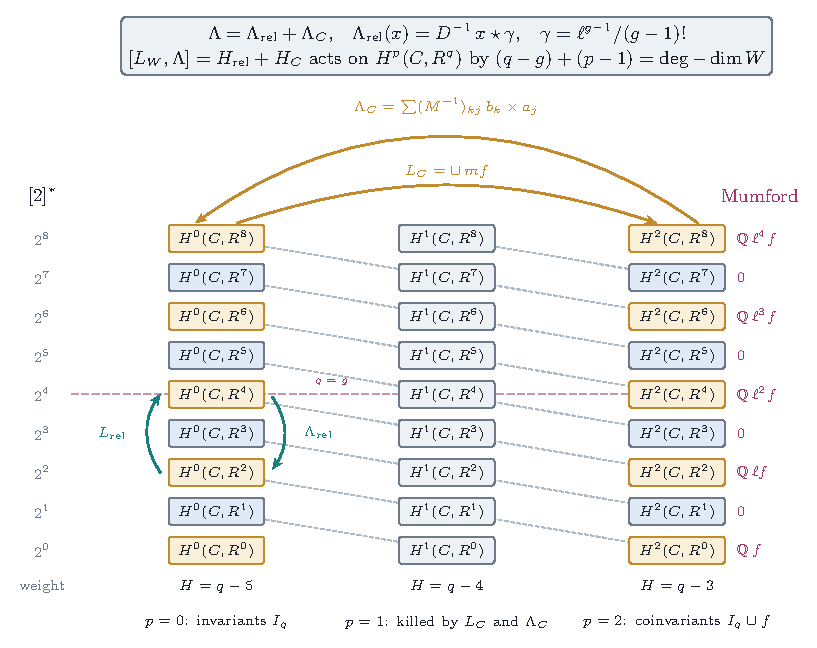
\includegraphics[width=0.86\textwidth]{fig_lefschetzgrid}
\caption{The proof of \Cref{thm:lefschetzfamily} for relative dimension
four. The boxes are the summands $H^{p}(C,R^{q}\pi_{*}\QQ)$ of $H^{*}(W,\QQ)$,
split off by the eigenvalue $2^{q}$ of $[2]^{*}$ shown on the left; the dotted
diagonals join the summands of one $H^{k}(W,\QQ)$, $k=p+q$, and the dashed
magenta line is the axis $q=g$ of hard Lefschetz on the fibres. The relative
operators $L_{\mathrm{rel}}$ and $\Lambda_{\mathrm{rel}}$, in teal, move
within a column; $\Lambda_{\mathrm{rel}}$ is a Pontryagin product with an
algebraic class on every abelian scheme (\Cref{prop:pontryaginlambda}). The
base operators $L_{C}$ and $\Lambda_{C}$, in ochre, move along a row between
the outer columns and kill the middle one; $\Lambda_{C}$ is the displayed
cycle built from bases $(a_{j})$, $(b_{k})$ of the invariant summands, and is
algebraic exactly when the invariant cycles are. Below each column is the
weight of $H=[L_{W},\Lambda]$ on it, and the panel at the top is Step 6 of the
proof. The ochre boxes carry the invariant cycles and their images under
$L_{C}$; for a Mumford family they are the lines listed in magenta on the
right, spanned by $\ell^{i}f$ (and by $\ell^{i}$ in the left column), and the
other boxes of the outer columns are zero (\Cref{cor:mumfordlefschetz}).}
\label{fig:lefschetzgrid}
\end{figure}

\begin{remark}[What this does and does not reach]\label{rem:newlefschetzscope}
The total space $W$ is a fivefold fibred in abelian fourfolds whose Hodge
groups are not defined by endomorphisms; it is not a product and not an
abelian variety. For abelian schemes over curves the mechanism of
\Cref{thm:lefschetzfamily} goes back to Tankeev \cite{Tan03}, who proves $B$
for the total space when certain canonically defined Hodge cycles are
algebraic; we have not checked whether his hypotheses are visibly met by
Mumford families, and make no claim of priority for
\Cref{cor:mumfordlefschetz}. The
hypothesis of \Cref{thm:lefschetzfamily} is where the difficulty sits.
Applied to the fibre square $W\times_{C}W\to C$ the theorem gives
$B(W\times_{C}W)$ as soon as every invariant class of $X\times X$ is the
restriction of an algebraic class on $W\times_{C}W$; the invariant classes
include the two exceptional classes of \Cref{prop:mumfordproduct}, which are
not known to be algebraic, so this is the smallest case of (F2) in a global
form. \Cref{thm:lefschetzfamily} does not bear on (P2), on the Kuga--Satake
class of \Cref{thm:mumfordks}, or on \textup{(L)} for varieties that are not
fibred in abelian varieties over a curve.
\end{remark}

\begin{proposition}[Powers of a Weil variety; cf.\ \cite{Mil22}]\label{prop:powers}
Let $X$ be of $(K,-1,n)$-Weil type with $n\ge2$ and $\Hg(X)=\SU(V,H)$. For
every $k\ge1$ the $\QQ$-algebra $\Hdg^{*}(X^{k})$ is generated by the divisor
classes of $X^{k}$ and the pull-backs $f_{a}^{*}\omega$ of the Weil classes
$\omega$ of $X$ along the homomorphisms $f_{a}=\sum_{j}a_{j}\,pr_{j}\colon
X^{k}\to X$, $a\in\ZZ^{k}$. Consequently, if the Weil classes of $X$ are
algebraic, the Hodge conjecture holds for every power of $X$. By
\cite{Mar25a} this is so for every such $X$ with $n=2$, and with $n=3$ and
trivial discriminant.
\end{proposition}

\begin{proof}
Write $H^{1}(X,\CC)=V_{+}\oplus V_{-}$ for the eigenspaces of $K$ and
$W=V_{+}$. The polarisation makes $V_{+}$ and $V_{-}$ isotropic and pairs them
perfectly, so $V_{-}=W^{\vee}$, and restriction to $V_{+}$ identifies
$\SU(V,H)_{\CC}$ with $\SL(W)$. As $\Hg(X^{k})$ is $\Hg(X)$ acting diagonally
on $H^{1}(X^{k},\CC)=(W\otimes U)\oplus(W^{\vee}\otimes U)$, $U=\CC^{k}$, the
Hodge classes of $X^{k}$, tensored with $\CC$, are the $\SL(W)$-invariants in
$\bigwedge^{*}\bigl((W\otimes U)\oplus(W^{\vee}\otimes U)\bigr)$. That algebra
is an $\SL(W)$-equivariant quotient of a tensor algebra, with an equivariant
section given by antisymmetrisation, so by the first fundamental theorem of
invariant theory for $\SL(W)$ its invariants are generated by the images of
the contractions and the determinant tensors: the classes
$D(u,u')=\sum_{i}(e_{i}\otimes u)\wedge(e_{i}^{\vee}\otimes u')$ and the
polarised determinants, which by polarisation are combinations of
$\det_{u}=\bigwedge_{i}(e_{i}\otimes u)$ and
$\det^{\vee}_{u}=\bigwedge_{i}(e_{i}^{\vee}\otimes u)$, $u,u'\in U$. For
$2n\ge3$ the $D(u,u')$ span the invariants of degree two, which are the
divisor classes tensored with $\CC$. With $\alpha_{\pm}$ spanning
$\bigwedge^{2n}V_{\pm}$ (\Cref{prop:weilline}) one has
$f_{a}^{*}\alpha_{+}=\det_{a}$ and $f_{a}^{*}\alpha_{-}=\det^{\vee}_{a}$, and
since $u\mapsto\det_{u}$ is polynomial and $\ZZ^{k}$ is Zariski dense in
$U$, these span the same space as all $\det_{u}$. So the $\QQ$-algebra
generated by $\NS(X^{k})_{\QQ}$ and the $f_{a}^{*}\omega$ is contained in
$\Hdg^{*}(X^{k})$ and has the same complexification. The generators are
algebraic when the Weil classes of $X$ are, and they are for $n=2$ and for
$n=3$ at trivial discriminant by \cite{Mar25a}.
\end{proof}

The statement for powers is known (compare \cite{Mil22}, and \cite{Li26} for
the powers of CM fourfolds); we include the short proof because it is what
the next corollary uses.

\begin{corollary}[Abelian schemes of small relative dimension]
\label{cor:lefschetzsmall}
Let $\pi\colon W\to C$ be an abelian scheme of relative dimension $g$ over a
smooth projective connected curve, with $W$ projective, and suppose that
every monodromy invariant class in $H^{*}(W_{c},\QQ)$ is a Hodge class, as
happens when the identity component of the Zariski closure of the monodromy
group is the Hodge group of a very general fibre.
\begin{enumerate}[label=\textup{(\roman*)},leftmargin=2.6em,itemsep=2pt]
\item If $g\le4$, then $B(W)$ holds.
\item If the fibres are of $(K,-1,n)$-Weil type with connected monodromy
  group $\SU(V,H)$, and $n=2$, or $n=3$ with trivial discriminant, then
  $B$ holds for every fibre power $W\times_{C}\dots\times_{C}W$. In
  particular $B(W_{C})$ of \Cref{cor:weilequiv} holds in these cases.
\end{enumerate}
\end{corollary}

\begin{proof}
By the theorem of the fixed part the invariant classes form a sub-Hodge
structure of every fibre, with a Hodge structure independent of the point, so
they are Hodge classes on every fibre. (i) The Hodge conjecture holds for
abelian varieties of dimension at most four, by the Lefschetz theorem on
$(1,1)$ classes and hard Lefschetz up to dimension three and by \cite{Mar25a}
in dimension four, so each invariant
class is algebraic on every fibre; \Cref{lem:spreading} makes it the
restriction of an algebraic class on $W$, and \Cref{thm:lefschetzfamily}
applies. (ii) The fibre power is an abelian scheme with projective total
space and the monodromy acting diagonally. Its invariant classes are
$\SU(V,H)$-invariants, hence Hodge classes at every member with
$\Hg=\SU(V,H)$, an uncountable set of points, and there the Hodge conjecture
holds for the fibre by \Cref{prop:powers}; \Cref{lem:spreading} and
\Cref{thm:lefschetzfamily} conclude as before. For $W_{C}$ the connected
monodromy group is $\SU(V,H)$ when it is Zariski dense, which is the
hypothesis of \Cref{cor:weilequiv}(ii).
\end{proof}

\begin{proposition}[The total space of a Mumford family]
\label{prop:mumfordfivefold}
Let $W\to C$ be as in \Cref{cor:mumfordlefschetz}, with $C$ the compact
Shimura curve of \cite{Mum69} of torsion-free level, or a finite \'etale cover
of it. Then the Hodge conjecture holds for the fivefold $W$: its Hodge classes
of degree $2p$ are spanned by $\ell^{p}$ and $f\ell^{p-1}$, with $f$ the class
of a fibre.
\end{proposition}

\begin{proof}
By Step 1 of the proof of \Cref{thm:lefschetzfamily},
$H^{k}(W,\QQ)=\bigoplus_{q}H^{k}_{(q)}$ with $H^{k}_{(q)}\cong
H^{k-q}(C,R^{q}\pi_{*}\QQ)$, the summands being sub-Hodge structures cut out by
algebraic projectors. The summand with $k=q$ is the space of invariants, which
by the proof of \Cref{cor:mumfordlefschetz} is spanned by the powers of the
polarisation, restrictions of the powers of $\ell$. The summand with $k=q+2$
is $f\cup H^{q}_{(q)}$ by Step 5, spanned by the $f\ell^{q/2}$. It remains to
see that $H^{1}(C,R^{q}\pi_{*}\QQ)$ carries no Hodge class. For $q$ even its
weight $q+1$ is odd. For $q$ odd, over $\CC$ the local system splits as a sum
of $S^{k_{1}}V_{1}\otimes U_{\lambda}\otimes M_{\lambda}$, where $V_{1}$ is the
uniformising variation of the factor of $G$ split at the real place, $U_{\lambda}$ is
a unitary variation of type $(0,0)$, $M_{\lambda}$ is constant of type $(a,a)$
with $2a+k_{1}=q$, and $k_{1}\equiv q\pmod2$ because the central element
$(-1,1,1)$ acts on $V$ by $-1$. When $C$ is \'etale over the Shimura curve the
Kodaira--Spencer map of $V_{1}$ is an isomorphism, and then
$H^{1}(C,S^{k_{1}}V_{1}\otimes U_{\lambda})$ has only the types $(k_{1}+1,0)$
and $(0,k_{1}+1)$ \cite{Zuc79}; after the twist by $M_{\lambda}$ these are
never balanced, since $k_{1}\ge1$.
\end{proof}

We have not found \Cref{prop:mumfordfivefold} in the literature, but it is of a
kind studied for Kuga fibre varieties and we make no claim of priority. The
\'etale hypothesis cannot be dropped from the argument: over a ramified cover
the Kodaira--Spencer map has zeros and balanced types can occur in
$H^{1}(C,R^{q}\pi_{*}\QQ)$.

\subsection{The two remaining targets, each reduced to one case of (L)}
\label{ssec:targets}

The machinery of \Cref{ssec:newlefschetz} does more than add a case of
\textup{(L)}. For an abelian scheme over a curve it shows that \textup{(L)}
for the total space is exactly the statement that algebraicity propagates
along the curve, and the base points of this paper then turn each of the two
targets left open in \Cref{rem:bullseye}, one Weil family and the first
classes beyond the Weil lines, into \textup{(L)} for one explicit variety. The
reductions are equivalences, so they locate the difficulty rather than remove
it. Along the way two things are proved outright: the Hodge conjecture for the
self-product of a Mumford fourfold at every CM point, and the impossibility of
realising the two branches of \Cref{rem:twobranches} by two objects.

\begin{lemma}[Spreading along a curve]\label{lem:spreading}
Let $\pi\colon W\to C$ be a smooth projective morphism onto a smooth projective
connected curve, $W$ projective, and $\xi$ a global section of
$R^{2p}\pi_{*}\QQ$. If $\xi_{t}$ is algebraic for uncountably many $t\in C$,
there are an algebraic class $\tilde\xi$ on $W$ and an integer $d\ge1$ with
$\tilde\xi|_{W_{t}}=d\,\xi_{t}$ for every $t\in C$.
\end{lemma}

\begin{proof}
The proof of \Cref{thm:closedlocus} applies verbatim with $(\cA,\cS,\omega)$
replaced by $(W,C,\xi)$: the set of $t$ at which $\xi_{t}$ is algebraic is
the union, over countably many tuples of Hilbert polynomials and rational
coefficients, of the images of unions $T$ of connected components of fibre
products of relative Hilbert schemes, projective over $C$, on which
$\sum_{i}q_{i}[Z_{i}]=\xi$. Uncountably many $t$ force one image to be
infinite, hence equal to $C$. Choose an irreducible component of that $T$
surjecting onto $C$, two of its points over distinct points of $C$, and an
irreducible curve through them; its normalisation $C'$ maps finitely onto $C$,
of some degree $d$. Pulling the universal subschemes back to
$W'=W\times_{C}C'$ gives a cycle $z=\sum_{i}q_{i}[\cZ_{i}]$ whose restriction
to $W'_{c'}=W_{g(c')}$ is $\xi_{g(c')}$ for every $c'\in C'$. The projection
$h\colon W'\to W$ is finite and flat of degree $d$, and by base change
$h_{*}[z]$ restricts on $W_{t}$ to the sum of the restrictions over the
points of $C'$ above $t$, counted with multiplicity, which is $d\,\xi_{t}$.
\end{proof}

\begin{theorem}[\textup{(L)} for an abelian scheme over a curve is
propagation]\label{thm:lefschetzpropagation}
Let $\pi\colon W\to C$ be as in \Cref{thm:lefschetzfamily}, but with no
hypothesis on its invariant cycles, and keep the notation of its proof. Let
$\Lambda_{C}$ be the operator that is zero on $H^{p}(C,R^{q}\pi_{*}\QQ)$ for
$p\ne2$ and inverts $L_{C}\colon H^{q}_{(q)}\to H^{q+2}_{(q)}$.
\begin{enumerate}[label=\textup{(\roman*)},leftmargin=2.6em,itemsep=2pt]
\item The operator $\Lambda$ of \Cref{def:Bconj} for $L_{W}$ is
  $\Lambda_{\mathrm{rel}}+\Lambda_{C}$. So $B(W)$ holds for $L_{W}$ if and
  only if $\Lambda_{C}$ is induced by an algebraic cycle.
\item If $B(W)$ holds for $L_{W}$, then for every $c\in C$ and every algebraic
  class $y$ on $W_{c}$ the class $\Lambda_{C}(i_{c*}y)$ is algebraic; up to
  the factor $m$ it lies in $H^{0}(C,R^{q}\pi_{*}\QQ)$ and restricts on
  $W_{c}$ to the unique monodromy invariant class $v$ with
  $\int_{W_{c}}v\cup w=\int_{W_{c}}y\cup w$ for every invariant $w$ of
  complementary degree. In particular every global section of
  $R^{2p}\pi_{*}\QQ$ that is algebraic at one point is the restriction of an
  algebraic class on $W$, and is algebraic at every point.
\item If at one point $c_{0}$ every monodromy invariant class of
  $H^{*}(W_{c_{0}},\QQ)$ is algebraic, then $B(W)$ holds for $L_{W}$ if and
  only if every monodromy invariant class is the restriction of an algebraic
  class on $W$.
\end{enumerate}
\end{theorem}

\begin{proof}
(i) Steps 4 and 5 of the proof of \Cref{thm:lefschetzfamily} show that
$L_{C}\colon H^{q}_{(q)}\to H^{q+2}_{(q)}$ is an isomorphism without using
the hypothesis on invariant cycles: the nondegeneracy of
$I_{q}\times I_{2g-q}\to\QQ$ comes from the Hodge--Riemann relations alone.
So $\Lambda_{C}$ is defined, and Steps 5 and 6, which use only that
$\Lambda_{C}$ vanishes off $p=2$ and inverts $L_{C}$, give
$[L_{W},\Lambda_{\mathrm{rel}}+\Lambda_{C}]=H$. By the uniqueness in
\Cref{def:Bconj} this is $\Lambda$. As $\Lambda_{\mathrm{rel}}$ is induced by
an algebraic cycle (Step 3), $\Lambda$ is if and only if $\Lambda_{C}$ is.

(ii) The Gysin map $i_{c*}$ commutes with $[2]_{*}$, which acts on
$H^{q}(W_{c})$ by $2^{2g-q}$, so $i_{c*}y\in H^{q+2}_{(q)}$, the summand with
$p=2$. If $y$ is algebraic so is $i_{c*}y$, and by (i) so is
$\Lambda_{C}(i_{c*}y)$. Put $u=m\,\Lambda_{C}(i_{c*}y)\in H^{q}_{(q)}$, so
$f\cup u=i_{c*}y$. For $w\in H^{2g-q}_{(2g-q)}$ the projection formula gives
$\int_{W_{c}}u|_{W_{c}}\cup w|_{W_{c}}=\int_{W}(f\cup u)\cup w
=\int_{W}i_{c*}y\cup w=\int_{W_{c}}y\cup w|_{W_{c}}$, and $w|_{W_{c}}$ runs
over the invariants of complementary degree (Step 4); by the nondegeneracy of
Step 4 this determines $u|_{W_{c}}$. If $y=\xi_{c}$ for a global section
$\xi$, then $v=\xi_{c}$ has the property, so $u|_{W_{c}}=\xi_{c}$, and $u$,
being a global section of $R^{q}\pi_{*}\QQ$ equal to $\xi$ at $c$, restricts
to $\xi_{t}$ at every $t$.

(iii) If every invariant class is a restriction of an algebraic class, $B(W)$
holds by \Cref{thm:lefschetzfamily}. Conversely, under $B(W)$, (ii) applied at
$c_{0}$ to each invariant class makes it the restriction of an algebraic
class.
\end{proof}

\begin{figure}[tbp]
\centering
  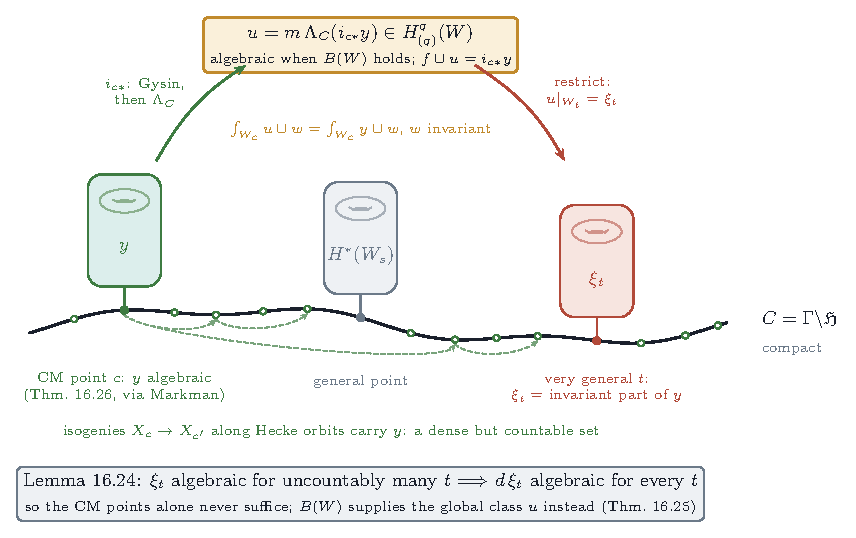
\includegraphics[width=0.84\textwidth]{fig_propagation}
\caption{\Cref{thm:lefschetzpropagation}(ii) along a compact Shimura curve
$C$. An algebraic class $y$ on one fibre, at a base point of a Weil family or
at a CM point of a Mumford family (hollow dots: the CM points, countable and
dense), is pushed into $W$ by the Gysin map and brought back to the invariant
summand by the base operator $\Lambda_{C}$. When $B(W)$ holds the result $u$
is an algebraic class on $W$, pinned down by the displayed pairing against the
invariant classes, and its restriction to a very general fibre is the
invariant part of $y$. The dashed arcs are isogenies between CM members along
Hecke orbits: they carry algebraic classes to algebraic classes but reach
only countably many points, and \Cref{lem:spreading}, in the box, needs
uncountably many. This is how \Cref{cor:weilequiv} and
\Cref{cor:mumfordequiv} turn each target into one case of \textup{(L)}.}
\label{fig:propagation}
\end{figure}

\begin{theorem}[The Mumford square at a CM point]\label{thm:mumfordcm}
Let $W\to C$ be a family as in \Cref{cor:mumfordlefschetz} and $c\in C$ a CM
point. Then every Hodge class on $X_{c}\times X_{c}$ is algebraic. In
particular the two exceptional classes of \Cref{prop:mumfordproduct} are
algebraic on $X_{c}\times X_{c}$.
\end{theorem}

\begin{proof}
The Hodge group $T$ of $X_{c}$ is a $\QQ$-torus contained in $G$. It lies in a
maximal $\QQ$-torus of $G=\Res_{F/\QQ}\SL_{1}(D)$, which is the restriction of
scalars of the norm one torus of a quadratic extension of $F$ inside $D$, of
rank three, one factor for each embedding of $F$. The cocharacter of the Hodge
structure lies in the factor of the embedding at which $D$ splits, and the
Galois group permutes the embeddings of $F$ transitively, so the smallest
$\QQ$-subtorus containing it has rank three: $T_{\CC}$ is a maximal torus of
$G_{\CC}\cong\SL_{2}^{3}$. Its eight weights on
$V=H^{1}(X_{c},\CC)=V_{1}\otimes V_{2}\otimes V_{3}$ are the vectors
$(\pm1,\pm1,\pm1)$, pairwise distinct. Hence
$\End^{0}(X_{c})\otimes\CC=\End_{T}(V)$ is the algebra of diagonal matrices
in a weight basis, $\operatorname{Hom}(X_{c}\times X_{c},X_{c})\otimes\CC$ is
the space of pairs $(\varphi,\psi)$ of such matrices acting by
$e_{w}\mapsto\varphi_{w}e_{w}^{(1)}+\psi_{w}e_{w}^{(2)}$, and the Hodge
classes of $X_{c}$ and of $X_{c}\times X_{c}$, tensored with $\CC$, are
spanned by the monomials of weight zero.

Item (XLIII) of \Cref{sec:verification} shows that the ring generated by the
divisor classes of $X_{c}\times X_{c}$ and by the pull-backs $f^{*}(t)$, for
$f=(\varphi,\psi)$ and $t$ a Hodge class of $X_{c}$ of degree $4$ or $6$,
contains every Hodge class of $X_{c}\times X_{c}$, in every degree. The map
$f\mapsto f^{*}(t)$ is polynomial and the rational homomorphisms are Zariski
dense in their complexification, so the same span is reached with $f$ defined
over $\QQ$ and $t$ rational. Divisor classes are algebraic, and the Hodge
classes of the abelian fourfold $X_{c}$ are algebraic because the Hodge
conjecture holds for abelian fourfolds \cite{Mar25a}; pull-backs and products
of algebraic classes are algebraic.
\end{proof}

\begin{corollary}[The first classes beyond the Weil lines are one case of
\textup{(L)}]\label{cor:mumfordequiv}
Let $W\to C$ be as in \Cref{cor:mumfordlefschetz} and
$W^{(2)}=W\times_{C}W\to C$, an abelian scheme of relative dimension eight
with $W^{(2)}$ projective of dimension nine. The following are equivalent.
\begin{enumerate}[label=\textup{(\alph*)},leftmargin=2.6em,itemsep=2pt]
\item $B(W^{(2)})$ holds for the class $L_{W^{(2)}}$.
\item The two exceptional classes of $X_{t}\times X_{t}$ are algebraic for
  uncountably many $t\in C$.
\item The Hodge conjecture holds for $X_{t}\times X_{t}$ for every $t\in C$.
\item The Hodge conjecture holds for $W^{(2)}$; for this item $C$ is taken to
  be the compact Shimura curve of torsion-free level, or a finite \'etale
  cover of it.
\end{enumerate}
\end{corollary}

\begin{proof}
As in the proof of \Cref{cor:mumfordlefschetz}, the connected monodromy group
is $G$, so the monodromy invariants in $H^{*}(X_{t}\times X_{t},\QQ)$ are
contained in the $G$-invariants, which are the Hodge classes of
$X_{t}\times X_{t}$ for $t$ very general; conversely a $G$-invariant class is
flat, being fixed by the monodromy. Item (XLIII) shows that these invariants
form a ring generated by its elements of degree two, the divisor classes, and
of degree four, which are the six products of divisor classes and the two
exceptional classes.

(c) implies (b) trivially. (b) implies (a): the exceptional classes are
restrictions of algebraic classes on $W^{(2)}$ by \Cref{lem:spreading}; so are
the invariant divisor classes, which are algebraic on every fibre, by the
same lemma; hence so is every invariant class, a polynomial in these, and
\Cref{thm:lefschetzfamily} gives $B(W^{(2)})$. (a) implies (c): at a CM point
$c_{0}$ every Hodge class of $X_{c_{0}}\times X_{c_{0}}$ is algebraic by
\Cref{thm:mumfordcm}, so by \Cref{thm:lefschetzpropagation}(iii) every
invariant class is the restriction of an algebraic class, and is algebraic on
every fibre. At a CM point (c) is \Cref{thm:mumfordcm}. At any other point
$t$ the Hodge group of $X_{t}$ is $G$, so its Hodge classes are the
invariant ones. Indeed, if the Hodge group $H_{t}$ were smaller, the Hodge
classes of the powers of $X_{t}$ that are not $G$-invariant would stay Hodge
only on a discrete subset of the period domain, the upper half plane; every
point of the orbit of the Hodge structure at $t$ under $H_{t}(\RR)^{+}$
carries them, so that orbit is a point, the cocharacter of
the Hodge structure is central in $H_{t}$, and $H_{t}$, the smallest
$\QQ$-group containing it, is a torus: $t$ would be a CM point.

For (d), split $H^{*}(W^{(2)},\QQ)$ into the summands $H^{p}(C,R^{q})$,
$p\in\{0,1,2\}$, as in the proof of \Cref{prop:mumfordfivefold}. The summands
with $p=1$ carry no Hodge class, by the argument given there, applied to the
fibre square. Those with $p=2$ are $f\cup H^{q}_{(q)}$, and
$f\cup u=i_{c*}(u|_{W^{(2)}_{c}})$ for any $c$; taking $c$ a CM point, where
$u|_{W^{(2)}_{c}}$ is a Hodge class and so algebraic by \Cref{thm:mumfordcm},
they are algebraic. The summands with $p=0$ are the invariants, all of Hodge
type. So (d) holds exactly when every invariant class is the restriction of an
algebraic class, which by \Cref{thm:lefschetzpropagation}(iii), applied at a
CM point, is (a).
\end{proof}

\begin{corollary}[One Weil family is one case of \textup{(L)}]
\label{cor:weilequiv}
Keep \Cref{setup:shimura}, let $s_{0}\in\cS$ be the image of a base point of
\Cref{thm:everyfamily}, and let $t_{1}\in\cS$ lie outside every proper
Zariski closed set $\Sigma_{\underline{P},\underline{q}}$ of
\Cref{thm:closedlocus}. Let $\kappa\colon C\to\cS$ be a morphism from a smooth
projective connected curve whose image contains $s_{0}$ and $t_{1}$, and
$W_{C}=\cA\times_{\cS}C$.
\begin{enumerate}[label=\textup{(\roman*)},leftmargin=2.6em,itemsep=2pt]
\item If $B(W_{C})$ holds for $L_{W_{C}}$, then $\Sigma=\cD_{n,n}$, and the
  Hodge conjecture holds in every degree for every member of the family with
  $\Hg(A)=\SU(V,H)$.
\item Conversely, if $\Sigma=\cD_{n,n}$ and the monodromy of $W_{C}$ is Zariski
  dense in $\SU(V,H)$, then $B(W_{C})$ holds for $L_{W_{C}}$.
\end{enumerate}
\end{corollary}

\begin{proof}
(i) The class $\kappa^{*}\omega$ is a global section of
$R^{2n}\pi_{*}\QQ$ on $C$, algebraic at a point over $s_{0}$ by
\Cref{thm:everyfamily}. By \Cref{thm:lefschetzpropagation}(ii) it is algebraic
at a point over $t_{1}$, so $t_{1}$ lies in some closed set
$\Sigma_{\underline{P},\underline{q}}$, which is therefore all of $\cS$.
\Cref{thm:closedlocus} gives $\Sigma=\cD_{n,n}$, and \Cref{thm:residual}(a)
the rest. (ii) With dense monodromy the invariants are the
$\SU(V,H)$-invariants, which are the Hodge classes of a member with
$\Hg(A)=\SU(V,H)$: the powers of the polarisation and the Weil classes, by
\Cref{thm:hdgcount}. All are algebraic on every fibre when
$\Sigma=\cD_{n,n}$, so they are restrictions of algebraic classes by
\Cref{lem:spreading}, and \Cref{thm:lefschetzfamily} applies.
\end{proof}

Curves $\kappa$ as in \Cref{cor:weilequiv} exist: the Baily--Borel
compactification of $\cS$ is projective \cite{BB66}, its boundary has
codimension $2n-1\ge3$, the rational boundary components of the domain of type
$\mathrm{I}_{n,n}$ being of type $\mathrm{I}_{n-r,n-r}$ with $r\ge1$, and a
general complete intersection curve through $s_{0}$ and $t_{1}$ avoids it.

\begin{theorem}[Two branches cannot be two objects]\label{thm:nosum}
Let $A$ be of $(K,-1,n)$-Weil type with $n\ge2$, $\omega\ne0$ a rational class
on the Weil line, and $E$ a perfect complex with $\ch(E)=N\omega$, $N\ne0$, and
$\sigma_{E}$ injective, for instance with $\dim\Ext^{2}(E,E)=2n(2n-1)$. Let
$E\cong\bigoplus_{i}F_{i}[k_{i}]$ be any decomposition. Then every summand
$F_{i}$ with $\ch(F_{i})\ne0$ has a Yoneda product
$\bigwedge^{2}\Ext^{1}(F_{i},F_{i})\to\Ext^{2}(F_{i},F_{i})$ that is not
injective. In particular $E$ is not a direct sum of shifts of line bundles,
of skyscraper sheaves of points, or of their images under autoequivalences of
$D^{b}(A)$, since the Ext algebra of each of these is the exterior algebra on
its $\Ext^{1}$.
\end{theorem}

\begin{proof}
By \Cref{thm:p2numerical}(ii) the kernel of $\operatorname{ev}_{E}$ in degree
two is $P\wedge Q$. The characteristic morphism is compatible with the
decomposition, so $\operatorname{ev}_{F_{i}}(p\wedge q)=
\operatorname{ev}_{F_{i}}(p)\operatorname{ev}_{F_{i}}(q)=0$ for all
$p\in P$ and $q\in Q$. Suppose the Yoneda product of $F=F_{i}$ is injective on
$\bigwedge^{2}\Ext^{1}$. Then the images $\bar P$ and $\bar Q$ of $P$ and $Q$
in $\Ext^{1}(F,F)$ satisfy $\bar p\wedge\bar q=0$ for all $\bar p,\bar q$, so
either $\bar P=0$, or $\bar Q=0$, or $\bar P=\bar Q$ is a line. In the first
case $\operatorname{ev}_{F}$ kills $P\wedge HH^{1}$, in the second
$Q\wedge HH^{1}$, in the third all of $HH^{2}=HH^{1}\wedge HH^{1}$; by the
compatibility $\sigma_{F}\circ\operatorname{ev}_{F}=(\,\cdot\,)\lrcorner
\ch(F)$ of \Cref{setup:hh} the same subspace annihilates $x=\ch(F)$.

These annihilators are computed in the free module of rank one that
$H^{*}(A,\CC)$ is over $HH^{*}(A)=\bigwedge^{*}(P\oplus Q)$, with generator the
holomorphic volume form $\Omega$: an element $y\cdot\Omega$ is killed by
$P\wedge HH^{1}$ exactly when $p\wedge y$ has top degree for every $p\in P$,
that is when $y\in\det P\wedge\bigwedge^{*}Q+\bigwedge^{\ge4n-1}(P\oplus Q)$.
Since $\det P\cdot\Omega=\pm\alpha_{+}$, the first summand gives the classes
$\bigwedge^{j}Q\cdot\alpha_{+}$, of type $(n-b,n+a)$ with $a$ wedges by
$V_{-}^{0,1}$ and $b$ contractions by $T_{+}$, and the second gives classes of
type $(1,2n)$, $(0,2n-1)$ and $(0,2n)$. The components of $x$ are of type
$(k,k)$, so $x\in\CC\alpha_{+}$. Symmetrically the second case gives
$x\in\CC\alpha_{-}$ and the third $x=0$; item (XLIII) confirms the three
annihilators for $n\le3$, and so does the Lean certificate. Finally $x$ is
rational, complex conjugation carries $V_{+}$ to $V_{-}$ and $H^{1,0}$ to
$H^{0,1}$, so $\bar\alpha_{+}\in\CC\alpha_{-}$, and a rational multiple of
$\alpha_{+}$ or of $\alpha_{-}$ is zero. So $\ch(F)=0$. As
$\sum_{i}(-1)^{k_{i}}\ch(F_{i})=N\omega\ne0$, some summand has nonzero
Chern character, and the first statement follows; the second is the special
case in which every summand has an exterior Ext algebra.
\end{proof}

\begin{remark}[Where the two targets stand]\label{rem:targetsstatus}
\Cref{cor:weilequiv} and \Cref{cor:mumfordequiv} say that closing one Weil
family and closing the first classes beyond the Weil lines are each the
Lefschetz standard conjecture for one variety: the total space of the family
over a curve through a base point, and the ninefold $W\times_{C}W$. By
\Cref{thm:lefschetzpropagation} that case of \textup{(L)} is in turn the
algebraicity of the invariant cycles, so nothing is gained for free: the
reduction moves both targets onto the bullseye of \Cref{rem:bullseye} and
shows that they sit there, and no further. Some things are unconditional:
the Hodge conjecture for the total space of a Mumford family over its Shimura
curve (\Cref{prop:mumfordfivefold}), $B$ for every abelian scheme over a curve
of relative dimension at most four whose invariant classes are Hodge
(\Cref{cor:lefschetzsmall}), and the following two. The
Mumford classes are algebraic at every CM point (\Cref{thm:mumfordcm}), so the
first case of (F2) is a propagation problem along one compact Shimura curve,
exactly as a Weil family is a propagation problem from its base point. And the
object (P2) asks for cannot be assembled from two objects each of which sees
one branch (\Cref{thm:nosum}): the two branches of \Cref{rem:twobranches} must
live inside a single summand with a quadratic relation among its first order
deformations. Neither target is closed here. For the Mumford target
\Cref{ssec:mumfordrigid} goes further: it closes off degeneration and
deformation into a larger family, reduces semiregularity to one dimension,
$119$, and specialisation to a degree bound at CM points; and
\Cref{ssec:mumfordobject} closes off every construction from line bundles and
every twistor deformation of the square, and shows that modulo $p$ the
classes are represented at every closed point of every reduction, so that the
target there is a bound on those representatives (\Cref{thm:lefschetzclosure},
\Cref{prop:notwistor}, \Cref{thm:modpdensity}).

The logic runs one way only. $B(W_{C})$ and $B(W\times_{C}W)$ are two cases of
\textup{(L)}, not \textup{(L)}: \textup{(L)} for every variety implies both,
but both together close one Weil family and the first case of (F2) and
nothing more. The conjecture needs \textup{(L)} for every variety together
with \textup{(M)} (\Cref{prop:lefmot}), or (F3), which is the conjecture
itself (\Cref{prop:f3ishc}), and no case of \textup{(L)} proved or reduced in
this section bears on \textup{(M)} or on (F3).
\end{remark}

\subsection{What would close it, computed rather than listed}
\label{ssec:closure}

A list of open problems invites a reading it does not deserve, that each entry
is a step and that the steps together are a path. The implications proved
above, together with those of \Cref{ssec:bullseye}, decide the question, so
we settle it by computation instead of by description. The logical skeleton
of the paper and of the literature it quotes is finite: a set of statements,
each of them proved here, quoted from the literature, or open, and a set of
inference rules, each of them one theorem. Consequences can then be taken.

Such a computation is only as strong as its rule set. A set of statements
the rules do not carry to the conjecture is \emph{insufficient} in the sense
of the computation, and that means no more than that no rule derives the
conjecture from it. An implication that is true and left out makes the
computation report a set as necessary when it is not. One such implication
is elementary, and it decides the shape of the answer, so we prove it first.

\begin{proposition}[The conjecture for the varieties that are not abelian
is the conjecture]\label{prop:f3ishc}
Let $A$ be a complex abelian variety of dimension $g\ge1$ and let
$X=A\times\PP^{1}$. Then $X$ is a smooth complex projective variety that is
not an abelian variety, and if every Hodge class of degree $2p$ on $X$ is
algebraic, then so is every Hodge class of degree $2p$ on $A$. Consequently
the statement
\begin{quote}
the Hodge conjecture holds for every smooth complex projective variety that
is not an abelian variety
\end{quote}
implies the Hodge conjecture for every abelian variety, and it is equivalent
to $\mathbf{HC}$.
\end{proposition}

\begin{proof}
$X$ is smooth and projective of dimension $g+1$. By the K\"unneth formula
$h^{1,0}(X)=h^{1,0}(A)+h^{1,0}(\PP^{1})=g$, while an abelian variety of
dimension $g+1$ has $h^{1,0}=g+1$; so $X$ is not an abelian variety. (Equally,
$X$ contains the rational curves $\{a\}\times\PP^{1}$, and every morphism
from $\PP^{1}$ to a complex torus is constant, since it lifts to the
universal cover $\CC^{g+1}$ \cite[Chapter~1]{BL04}.)

Let $\mathrm{pr}\colon X\to A$ be the projection and $D=A\times\{0\}$, a
smooth divisor that $\mathrm{pr}$ maps isomorphically onto $A$, so that
$\mathrm{pr}_{*}[D]=1$ in $H^{0}(A,\QQ)$. Let $\alpha$ be a Hodge class of
degree $2p$ on $A$. Pull-back along a morphism is a morphism of Hodge
structures, so $\mathrm{pr}^{*}\alpha$ is a Hodge class of degree $2p$ on
$X$, and by hypothesis $\mathrm{pr}^{*}\alpha=[Z]$ for an algebraic cycle
$Z$ on $X$ with rational coefficients. The projection formula gives
\[
  \mathrm{pr}_{*}\bigl([Z]\cup[D]\bigr)
  =\mathrm{pr}_{*}\bigl(\mathrm{pr}^{*}\alpha\cup[D]\bigr)
  =\alpha\cup\mathrm{pr}_{*}[D]=\alpha .
\]
The cycle class map is compatible with intersection products and with proper
push-forward \cite[Chapter~19]{Ful98}, so the left side
is the class of the cycle $\mathrm{pr}_{*}(Z\cdot D)$ and $\alpha$ is
algebraic. A point, the abelian variety of dimension zero, satisfies the
conjecture trivially.

So the displayed statement gives the conjecture for every abelian variety,
and with it the conjecture for every smooth complex projective variety. The
converse is immediate: the displayed statement is a special case of
$\mathbf{HC}$.
\end{proof}

Since the conjecture for the varieties that are not abelian is the whole
conjecture, the statement that belongs on a frontier is weaker: it asks for
algebraicity only modulo what abelian varieties supply.

\begin{definition}[The conjecture modulo abelian varieties]
\label{def:f3prime}
For a smooth complex projective variety $X$ and $p\ge0$ let
$\mathrm{Ab}^{p}(X)\subseteq H^{2p}(X,\QQ)$ be the span of the classes
$\Gamma_{*}\gamma=\mathrm{pr}_{X*}\bigl([\Gamma]\cup\mathrm{pr}_{B}^{*}\gamma\bigr)$
of degree $2p$, where $B$ runs over the complex abelian varieties, the point
included, $\gamma$ over the Hodge classes on $B$, and $\Gamma$ over the
algebraic cycles on $B\times X$ with rational coefficients. The statement
\textup{(F3$'$)} is: for every $X$ and every $p$,
\[
  \Hdg^{p}(X)=\mathrm{Ab}^{p}(X).
\]
\end{definition}

Each $\Gamma_{*}\gamma$ is a Hodge class, since cup product with an
algebraic class and push-forward preserve Hodge classes, so
$\mathrm{Ab}^{p}(X)\subseteq\Hdg^{p}(X)$; and taking $B$ a point shows that
$\mathrm{Ab}^{p}(X)$ contains every algebraic class. So \textup{(F3$'$)} says
that every Hodge class is algebraic modulo the images of Hodge classes of
abelian varieties under algebraic correspondences, which is the form of (F3)
that \Cref{rem:f3collapse} asks for.

\begin{proposition}[What is known of \textup{(F3$'$)}]\label{prop:f3prime}
\leavevmode
\begin{enumerate}[label=\textup{(\roman*)},leftmargin=2.6em]
\item $\mathbf{HC}$ implies \textup{(F3$'$)}, and \textup{(F3$'$)} together
  with the conjecture for abelian varieties implies $\mathbf{HC}$.
\item \textup{(F3$'$)} holds on every abelian variety and on every product
  $A\times\PP^{1}$ with $A$ abelian; the argument of \Cref{prop:f3ishc} gives
  nothing for it.
\item Let $\mathcal{A}$ be the class of smooth complex projective varieties
  $X$ for which $H^{*}(X,\QQ)$ is spanned by classes $\Gamma_{*}y$ with $B$
  abelian, $\Gamma$ an algebraic cycle on $B\times X$ and
  $y\in H^{*}(B,\QQ)$. Every $X\in\mathcal{A}$ satisfies \textup{(F3$'$)}.
  The class $\mathcal{A}$ contains every abelian variety and every smooth
  projective curve, and it is closed under products and under images of
  surjective morphisms. So it contains every product of curves, every
  symmetric product of a curve, and every smooth projective variety onto
  which a product of curves or an abelian variety maps surjectively.
\item Every $X$ of dimension $n$ satisfies \textup{(F3$'$)} in the degrees
  $2p$ with $p\in\{0,1,n-1,n\}$, so every $X$ of dimension at most three
  satisfies it in every degree.
\end{enumerate}
\end{proposition}

\begin{proof}
(i) If $\mathbf{HC}$ holds, then $\Hdg^{p}(X)$ consists of algebraic classes,
which lie in $\mathrm{Ab}^{p}(X)$. Conversely, if the conjecture holds for
abelian varieties, every $\gamma$ in \Cref{def:f3prime} is algebraic, so
every $\Gamma_{*}\gamma$ is, since composition with a correspondence carries
algebraic classes to algebraic classes \cite[Chapter~16]{Ful98}; then
\textup{(F3$'$)} says that every Hodge class is algebraic.

(ii) On an abelian variety $A$ take $B=A$ and $\Gamma$ the diagonal. On
$X=A\times\PP^{1}$ the K\"unneth formula gives
$H^{*}(X,\QQ)=\mathrm{pr}^{*}H^{*}(A,\QQ)\oplus
\mathrm{pr}^{*}H^{*}(A,\QQ)\cup\eta$, with $\eta$ the class of a point of
$\PP^{1}$ pulled back to $X$, which is algebraic. The first summand is
$\Gamma_{*}H^{*}(A,\QQ)$ for $\Gamma$ the transpose of the graph of
$\mathrm{pr}$, and the second is $\Gamma'_{*}H^{*}(A,\QQ)$ for
$\Gamma'=\Gamma\cdot\mathrm{pr}_{X}^{*}\eta$. So $X\in\mathcal{A}$, and
(iii) applies.

(iii) Let $X\in\mathcal{A}$ and fix $p$. Since $H^{2p}(X,\QQ)$ is finite
dimensional, finitely many classes $\Gamma_{j*}y_{j}$ span it, and we may
take each $\Gamma_{j}$ of pure codimension $c_{j}$ on $B_{j}\times X$ and each
$y_{j}$ of pure degree $k_{j}$, with $k_{j}+2c_{j}-2\dim B_{j}=2p$. Then
$\Gamma_{j*}\colon H^{k_{j}}(B_{j},\QQ)\to H^{2p}(X,\QQ)$ is a morphism of
Hodge structures up to a Tate twist, and the sum of these maps is a
surjective morphism of polarisable Hodge structures onto $H^{2p}(X,\QQ)$.
Polarisable Hodge structures are semisimple, so its kernel has a complement
that is a sub-Hodge structure and maps isomorphically onto $H^{2p}(X,\QQ)$;
hence every Hodge class of degree $2p$ is the image of a Hodge class, that is
$\sum_{j}\Gamma_{j*}\gamma_{j}$ with each $\gamma_{j}$ a Hodge class on
$B_{j}$. So $\Hdg^{p}(X)=\mathrm{Ab}^{p}(X)$.

An abelian variety lies in $\mathcal{A}$ through its diagonal. A curve $C$
of genus $g\ge1$ lies in $\mathcal{A}$ through an Abel--Jacobi embedding
$\iota\colon C\to J(C)$: the transpose of its graph induces $\iota^{*}$,
which is an isomorphism on $H^{0}$ and $H^{1}$ and sends the class of the
theta divisor to $g$ times the class of a point, so it is surjective; the
projective line is the image of an elliptic curve under a double cover, and
is covered by the last closure property. For products, if $H^{*}(X_{i},\QQ)$
is spanned by the $\Gamma_{i*}y$, then by the K\"unneth formula
$H^{*}(X_{1}\times X_{2},\QQ)$ is spanned by the
$(\Gamma_{1}\times\Gamma_{2})_{*}(y_{1}\otimes y_{2})$, with
$\Gamma_{1}\times\Gamma_{2}$ an algebraic cycle on
$(B_{1}\times B_{2})\times(X_{1}\times X_{2})$. For images, let
$f\colon Y\to X$ be a surjective morphism with $Y\in\mathcal{A}$, let
$r=\dim Y-\dim X$ and let $h$ be an ample class on $Y$. The correspondence
$\Psi=[\Gamma_{f}]\cdot\mathrm{pr}_{Y}^{*}h^{r}$ on $Y\times X$ induces
$\Psi_{*}y=f_{*}(y\cup h^{r})$, and
$\Psi_{*}f^{*}x=x\cup f_{*}h^{r}=c\,x$ with $c>0$ the degree of $h^{r}$ on a
general fibre. So $\Psi_{*}$ is surjective, and $H^{*}(X,\QQ)$ is spanned by
the classes $(\Psi\circ\Gamma)_{*}y$, with $\Psi\circ\Gamma$ algebraic
\cite[Chapter~16]{Ful98}. A symmetric product of a curve is the image of a
power of it.

(iv) Every class of degree $0$ or $2n$ is algebraic, and every Hodge class of
degree $2$ is algebraic by the Lefschetz theorem on $(1,1)$ classes. For
$n\ge2$, the hard Lefschetz theorem makes cup product with $h^{n-2}$, for $h$
an ample class, an isomorphism $H^{2}(X,\QQ)\to H^{2n-2}(X,\QQ)$ of Hodge
structures up to a Tate twist, so every Hodge class of degree $2n-2$ is
$h^{n-2}$ times a Hodge class of degree $2$, and is algebraic. Algebraic
classes lie in $\mathrm{Ab}^{p}(X)$. When $n\le3$ every $p$ between $0$ and
$n$ is one of $0,1,n-1,n$.
\end{proof}

\begin{remark}[Why \textup{(F3$'$)} is not closed here]\label{rem:f3primeopen}
\textup{(F3$'$)} is the statement that the Hodge conjecture reduces to
abelian varieties along algebraic correspondences, and
\Cref{prop:f3prime} records what is known of such a reduction: the
varieties of $\mathcal{A}$, whose whole cohomology is reached from abelian
varieties by algebraic correspondences, and the degrees in which the
conjecture itself is known. The first degree in which it is not known in
general is degree four on fourfolds, for fourfolds not known to lie in
$\mathcal{A}$. The square $S\times S$ of a K3 surface is the standard
example. Its Hodge classes in $H^{2}(S)\otimes H^{2}(S)$ include the classes
that induce the Hodge endomorphisms of the transcendental lattice $T(S)$, and
$S\times S$ lies in $\mathcal{A}$ as soon as the Kuga--Satake embedding of
$T(S)$ is induced by an algebraic cycle, the Kuga--Satake Hodge conjecture for
$S$, which is not known in general: the transpose of such a cycle maps the
cohomology of the Kuga--Satake variety onto $T(S)$, and the rest of
$H^{*}(S,\QQ)$ is algebraic. The rational Hodge isometries are algebraic
\cite{Bus19}, but a real multiplication is not an isometry, and
\Cref{rem:mumfordks} meets exactly this obstacle for the surfaces
$S_{\lambda}$.

For varieties whose cohomology is not of abelian type the position is
starker. By \Cref{prop:noabeliantype} no correspondence moves the $H^{3}$ of a
very general quintic threefold into the cohomology of an abelian variety, so
such a variety does not lie in $\mathcal{A}$. That is no obstruction to
\textup{(F3$'$)} itself, since a Hodge class spans a Hodge structure of Tate
type, which is of abelian type, and nothing in Hodge theory forbids it from
lying in $\mathrm{Ab}^{p}(X)$. Nor is it a route: to put a Hodge class into
$\mathrm{Ab}^{p}(X)$ one must construct an algebraic cycle on $B\times X$
whose class carries it, which is the kind of construction the Hodge
conjecture asks for, now on $B\times X$ instead of on $X$. The methods of
this paper construct cycles on abelian varieties of Weil type and on nothing
else, so they give no case of \textup{(F3$'$)} outside $\mathcal{A}$. We
therefore leave it open, and \Cref{thm:closure} treats it as an open
statement.
\end{remark}

\begin{setupenv}[The rule set]\label{setup:rules}
Item (XXXIII) of \Cref{sec:verification} carries forty-two statements and
twenty-two rules; the propagation statement (P2) is carried family by
family, as (P2) for the split and for the other families of the imaginary
quadratic fields and of the fields of degree at least four. Each statement is marked proved in this paper, quoted from the
literature, or open. Each rule is a finite set of premises together with one
conclusion, and carries the label of the theorem of this paper that proves it;
\Cref{tab:rules} lists the rules whose conclusion is derived rather than
assumed. For a set $T$ of statements write $\Cn(T)$ for the least set that
contains $T$ and is closed under the rules, which exists because each rule has
a single conclusion and the consequence operator is therefore monotone. Write
$\mathbf{T}$ for the set of statements marked proved or quoted, and
$\mathbf{HC}$ for the Hodge conjecture for every smooth complex projective
variety. Call a set $S$ of open statements \emph{sufficient} if
$\mathbf{HC}\in\Cn(\mathbf{T}\cup S)$, and \emph{minimal} if no proper subset
of $S$ is sufficient.
\end{setupenv}

\begin{table}[htbp]
\centering
\small
\renewcommand{\arraystretch}{1.14}
\begin{tabular}{@{}>{\raggedright\arraybackslash}p{0.40\linewidth}>{\raggedright\arraybackslash}p{0.27\linewidth}l@{}}
\toprule
premises & conclusion & by \\
\midrule
the conjecture for abelian varieties, (F3)
  & $\mathbf{HC}$ & \Cref{ssec:closuremap} \\
(F3)
  & abelian varieties & \Cref{prop:f3ishc} \\
the conjecture for abelian varieties, (F3$'$)
  & $\mathbf{HC}$ & \Cref{prop:f3prime} \\
the Weil classes of every CM field, (F2)
  & abelian varieties & \Cref{ssec:closuremap} \\
$K$ imaginary quadratic, the fields of degree at least four
  & every CM field & \Cref{app:albert} \\
$\delta=\delta_{0}$, $\delta\ne\delta_{0}$
  & every discriminant & \Cref{prop:separate} \\
a base point, the reduction, the orbit, (P2) for the family
  & that family & \Cref{thm:semiregclosure} \\
the same three for a CM field of degree at least four, (P2) for the family
  & that family & \Cref{thm:cmpropagation} \\
its split families, its other families
  & the fields of degree at least four & \Cref{prop:cmweil} \\
$\delta=\delta_{0}$
  & $\delta\ne\delta_{0}$ & \Cref{prop:descent} \\
the split families of the fields of degree at least four
  & their other families; $\delta=\delta_{0}$ & \Cref{prop:descent} \\
a secant object in every dimension, Question 11.4
  & $\delta=\delta_{0}$ & \Cref{prop:splitgeom} \\
a Cohen--Macaulay support, smooth or singular
  & one secant object & \Cref{cor:disjointroutes} \\
one secant object, Question 11.4
  & $\mathbf{W}(K,4,\delta_{0})$ & \Cref{cor:markmancondition} \\
\midrule
(L), (M)
  & $\mathbf{HC}$ & \Cref{prop:lefmot} \\
(L), the deformation theorem for motivated classes
  & (V) & \Cref{prop:lefvhc} \\
(V), the accessibility of Hodge classes on abelian varieties
  & abelian varieties & \Cref{thm:vhcab} \\
\bottomrule
\end{tabular}
\caption{The rules of \Cref{setup:rules} whose conclusion is derived, with the
theorem that proves each; the rows for (P2) and for the Cohen--Macaulay
support each stand for two rules, the row for descent over the fields of
degree at least four for two, descent within a field and scalar extension
down to the imaginary quadratic fields, the second row is \Cref{prop:f3ishc},
which an earlier version of the set omitted, the third is
\Cref{prop:f3prime}(i) for the weaker statement (F3$'$) of
\Cref{def:f3prime}, the last three rows are the rules of
\Cref{ssec:bullseye}, one of whose conclusions, (V), is itself open, and the
one remaining rule records what the literature supplies on Weil classes. The
bounded criterion (P1) is absent: by
\Cref{thm:p1equivalent} it is equivalent to its own conclusion, so it is a
restatement and not a premise. Item (XXXIII) of
\Cref{sec:verification} carries the whole set as data and checks that every
label here is a label of this paper.}
\label{tab:rules}
\end{table}

\begin{theorem}[The closure of what is proved here]\label{thm:closure}
With the notation of \Cref{setup:rules}:
\begin{enumerate}[label=\textup{(\roman*)},leftmargin=2.6em]
\item $\mathbf{HC}\notin\Cn(\mathbf{T})$. Nothing in this paper, combined with the
  theorems it quotes, implies the Hodge conjecture.
\item There are exactly five minimal sufficient sets:
  \[
    \{\mathrm{F3}\},\quad\{\mathrm{L},\mathrm{M}\},\quad
    \{\mathrm{L},\mathrm{F3}'\},\quad\{\mathrm{V},\mathrm{F3}'\},\quad
    \{\mathrm{P2}_{\mathrm{split}},\mathrm{F2},\mathrm{F3}'\},
  \]
  with \textup{(L)}, \textup{(M)}, \textup{(V)} as in \Cref{def:lmv},
  \textup{(F2)}, \textup{(F3)} as in \Cref{cor:fourremain}, (F3$'$) as in
  \Cref{def:f3prime}, and $\mathrm{P2}_{\mathrm{split}}$ the propagation
  statement \textup{(P2)}, read in the corrected form of \Cref{rem:p2prime},
  for the split families of the CM fields of degree at least four. No
  minimal set contains \textup{(P2)} for an imaginary quadratic field or for
  a family of nontrivial discriminant: \Cref{prop:descent} derives those.
  The single open statement (F3) is sufficient, and it is equivalent to
  $\mathbf{HC}$ (\Cref{prop:f3ishc}); no other single open statement is.
  The sets $\{\mathrm{L},\mathrm{F3}\}$, $\{\mathrm{V},\mathrm{F3}\}$ and
  $\{\mathrm{P2}_{\mathrm{split}},\mathrm{F2},\mathrm{F3}\}$ are sufficient and
  not minimal. The last of the five is the only one with three elements and the
  only one whose derivation of $\mathbf{HC}$ uses a statement proved in this
  paper.
\item In each of the five, every element is necessary: removing any one
  leaves $\mathbf{HC}$ outside the closure.
\item The secant route lies in no minimal sufficient set. Granting both of its
  open demands, a secant object satisfying \eqref{eq:heisenberg} in every
  dimension and an affirmative answer to \cite[Question 11.4]{Mar25b}, puts
  $\mathbf{W}(K,n,\delta_{0})$ in the closure, and with it, by
  \Cref{prop:descent}, $\mathbf{W}(K,n,\delta)$ for every $\delta$; it leaves
  the Weil classes of the CM fields of degree at least four outside.
\item No statement proved in this paper rests, at any depth, on an open one,
  and the rule set is acyclic.
\item Every element of a minimal sufficient set other than
  $\mathrm{P2}_{\mathrm{split}}$ is a consequence of $\mathbf{HC}$, and $\{\mathrm{F3}\}$ and
  $\{\mathrm{L},\mathrm{M}\}$ are each equivalent to it; no implication from
  $\mathbf{HC}$ to \textup{(P2)} is known.
\item An earlier version of this theorem, over a rule set without
  \Cref{prop:descent}, stated in (iv) that the secant route stops at the
  trivial discriminant, and listed \textup{(P2)} for every family in the
  fifth set. Both came from the omission of the rules of
  \Cref{prop:descent}, and the five minimal sets are otherwise unchanged.
\end{enumerate}
\end{theorem}

\begin{proof}
The consequence operator is monotone, so $\Cn$ is computed by iterating the
one step map to a fixed point, and the set of subsets of the sixteen open
statements is finite. Item (XXXIII) of
\Cref{sec:verification} carries out the iteration and the exhaustive search
over all $2^{16}$ subsets of the sixteen open statements in exact arithmetic,
and Section 24 of the Lean certificate repeats (i), (ii), (iii) and (iv) in
the kernel, over the same rule set under the numbering recorded there,
checking in particular all sixteen single open statements and all one
hundred and twenty pairs. The content of the statement is the rule set itself, and every rule is
one of the theorems named in \Cref{tab:rules}. The sufficiency of (F3)
alone is the chain $\mathrm{(F3)}\Rightarrow$ abelian varieties by
\Cref{prop:f3ishc}, then abelian varieties $\wedge\,\mathrm{(F3)}
\Rightarrow\mathbf{HC}$; every sufficient set that contains (F3) and has
another element is therefore not minimal, and a sufficient set without
(F3) must reach $\mathbf{HC}$ through one of the two other rules with that
conclusion, \Cref{prop:lefmot} or \Cref{prop:f3prime}(i), the second of
which needs the conjecture for abelian varieties, reached by \textup{(V)},
by \textup{(L)} through \textup{(V)}, or by (P2) with (F2). For (vi):
\textup{(L)} follows from $\mathbf{HC}$ by \Cref{thm:equivalence},
\textup{(M)} by \Cref{prop:lefmot}, \textup{(V)} by \Cref{prop:lefvhc},
(F3$'$) by \Cref{prop:f3prime}(i), and (F2) and (F3) are special cases of
$\mathbf{HC}$.

In (iv), every base point the secant route produces is a member
$X\times\widehat{X}$, whose discriminant is trivial whatever $\beta$ is chosen
(\Cref{prop:splitgeom}(ii)); the deformation argument stays inside the family
of trivial discriminant, and it is \Cref{prop:descent}(i), not the
deformation, that carries the result to the other discriminants. It has no
base point over a field of degree at least four, so it reaches none of them.
\end{proof}

\begin{corollary}[The three statements, one of which is the
conjecture]\label{cor:fourremain}
The Hodge conjecture follows from the results of this paper together with the
following three statements. No rule of \Cref{setup:rules} derives it from
(F1) and (F2) together, and it follows from (F3) alone, which is equivalent
to it
(\Cref{prop:f3ishc}); so the list is not a reduction of the conjecture to
three smaller problems. With (F3) replaced by the weaker statement
\textup{(F3$'$)} of \Cref{def:f3prime}, the conjecture modulo abelian
varieties, the three statements (F1), (F2), \textup{(F3$'$)} still suffice,
and no rule of \Cref{setup:rules} derives the conjecture from a proper
subset of them.
\begin{enumerate}[label=\textup{(F\arabic*)},leftmargin=3.0em,itemsep=4pt]
\item \emph{One propagation statement, for every CM field.} \textup{(P2)},
  in the corrected form of \Cref{rem:p2prime}: at one base point of each
  Weil family of each CM field some perfect complex whose Chern character is
  a nonzero multiple of a rational Weil class plus a polynomial in the
  polarisation has injective semiregularity map. Its first form, with Chern
  character exactly a multiple of the Weil class, is false for every
  imaginary quadratic field and every $n\ge2$ (\Cref{thm:p2false}): such a
  complex would have to deform to non-algebraic Weil tori, whose coherent
  sheaves have no Chern character below the top degree. The corrected form
  closes
  $\mathbf{W}(K,n,\delta)$
  for every imaginary quadratic $K$, every $n$ and every $\delta$ at once, by
  \Cref{thm:semiregclosure}, and
  $\mathbf{W}(F,n,\delta)$ for every CM field $F$ of higher degree, by
  \Cref{thm:cmpropagation}, because those theorems put $\Sigma=\cD$, so the
  Weil class is algebraic at every member of the family and not only at the
  general one, and because \Cref{thm:everyfamily} and \Cref{thm:cmbasepoint}
  supply the base point in every one of those families. By
  \Cref{prop:descent} it is enough to have it for the split families of the
  CM fields of degree at least four, in infinitely many dimensions.
  \Cref{thm:p2forces}, \Cref{thm:p2support}, \Cref{thm:nosum},
  \Cref{thm:p2numerical} and \Cref{thm:p2endo} describe the object of the
  first form and are vacuous by \Cref{thm:p2false}; for the corrected form
  \Cref{thm:p2primenumber} computes the number that $\dim\Ext^{2}(E,E)$ has
  to reach, $7n^{2}-2n$ for a general shape. For one family its
  conclusion is equivalent to the Lefschetz standard conjecture for one
  variety (\Cref{cor:weilequiv}). The bounded criterion \textup{(P1)} is not a
  second form of the same demand: by
  \Cref{thm:p1equivalent} it is equivalent to the conclusion it was to imply,
  and \Cref{thm:p1forces} shows that the one cycle it could have been tested
  on, the transport of the base cycle, does not satisfy it.
\item \emph{The classes beyond the Weil lines.} Every Hodge class on an
  abelian variety that lies outside the subring generated by divisor classes
  and by Weil classes of quotients is algebraic. Through dimension five there
  is no such class \cite{MZ99}; in dimension eight there are
  (\Cref{prop:mumfordproduct}), so this is not a reduction of the conjecture
  for abelian varieties to Weil classes, which is false as a statement about
  Hodge rings: it is the conjecture for those classes. Its smallest case is
  brought down to one Kuga--Satake class in \Cref{thm:mumfordks}; it holds at
  every CM point (\Cref{thm:mumfordcm}), and on all members of a Mumford
  family it is equivalent to the Lefschetz standard conjecture for one
  ninefold (\Cref{cor:mumfordequiv}). Its classes are rigid along the base
  curve (\Cref{thm:mumfordrigid}), and one complex at one CM point with
  $\Ext^{2}$ of dimension $119$ would close it (\Cref{thm:mumfordnumerical}),
  as would a bound on the cycles that represent them at the closed points of
  the reductions of the curve modulo primes (\Cref{thm:modpdensity}).
\item \emph{The varieties that are not abelian.} The Hodge conjecture holds
  for every smooth complex projective variety that is not an abelian variety.
  This is the Hodge conjecture itself. The varieties it covers include
  $A\times\PP^{1}$ for every abelian variety $A$, and the conjecture for
  $A\times\PP^{1}$ gives it for $A$ (\Cref{prop:f3ishc}); so (F3) implies
  the conjecture for abelian varieties, hence (F1) and (F2), and hence
  $\mathbf{HC}$. Nor is it a reduction to abelian varieties in the other
  direction: no realisation of the cohomology of an arbitrary variety inside
  that of abelian varieties exists (\Cref{prop:noabeliantype}), and
  \Cref{thm:hyperplane} and \Cref{thm:returntrip} close the two routes
  through hyperplane sections that would be the natural candidates for one.
\end{enumerate}
\end{corollary}

\begin{proof}
The three together are sufficient by the derivation of \Cref{thm:closure},
and (F3) alone by \Cref{prop:f3ishc}. That (F1) and (F2) together are not
sufficient in the rule set is \Cref{thm:closure}(ii), since every minimal
sufficient set contains (F3), \textup{(F3$'$)} or \textup{(M)}; the
statement about (F1), (F2), \textup{(F3$'$)} is \Cref{thm:closure}(ii) and
(iii) for the last of the five minimal sets. The Weil classes of the CM
fields of degree at least four are not a fourth statement: they are derived
from (F1) by \Cref{thm:cmpropagation}. Nor is the bounded criterion a
premise, since by \Cref{thm:p1equivalent} it is a restatement of its own
conclusion.
\end{proof}

\begin{remark}[How the earlier count went wrong, and the wording of (F2)]
\label{rem:f3collapse}
An earlier version of this corollary said that the conjecture follows from
no proper subset of the three statements. That was a statement about a rule
set that used (F3) only through $\text{(abelian varieties)}\wedge
\text{(F3)}\Rightarrow\mathbf{HC}$ and did not contain the elementary rule
$\text{(F3)}\Rightarrow\text{(abelian varieties)}$ of \Cref{prop:f3ishc}.
The rule set can show that a set suffices; it cannot show that a set is
needed, except relative to the implications written into it.

The wording of (F2) has the same feature, one degree at a time. Let
$R(A)\subseteq H^{*}(A,\QQ)$ be the subring generated by divisor classes and
Weil classes of quotients. Suppose some Hodge class $\beta$ of degree $2p$ on
$A$ lies outside $R(A)$, and let $\alpha$ be any Hodge class of degree $2p$.
If $\alpha\notin R(A)$, (F2) makes it algebraic. If $\alpha\in R(A)$, then
$\alpha+\beta\notin R(A)$, because $R(A)$ is closed under subtraction, so
(F2) makes $\alpha+\beta$ and $\beta$ algebraic, and with them $\alpha$.
So in every degree in which (F2) says anything it is the whole conjecture for
that degree: on the square of a Mumford fourfold it gives every Hodge class of
$H^{4}$, the six products of divisor classes included. Whether (F2) alone
gives the conjecture for every abelian variety is not decided here, and
nothing depends on it: the rule set does not use such an implication, and
adding it would not change \Cref{thm:closure}(ii), since (F3) alone is
already sufficient.

The form of (F3) that is not the conjecture itself asks only for
algebraicity modulo classes coming from abelian varieties. It is
\textup{(F3$'$)} of \Cref{def:f3prime}; \Cref{prop:f3prime} says what is
known of it, and \Cref{rem:f3primeopen} why it is not closed.
\end{remark}

\begin{figure}[tbp]
\centering
  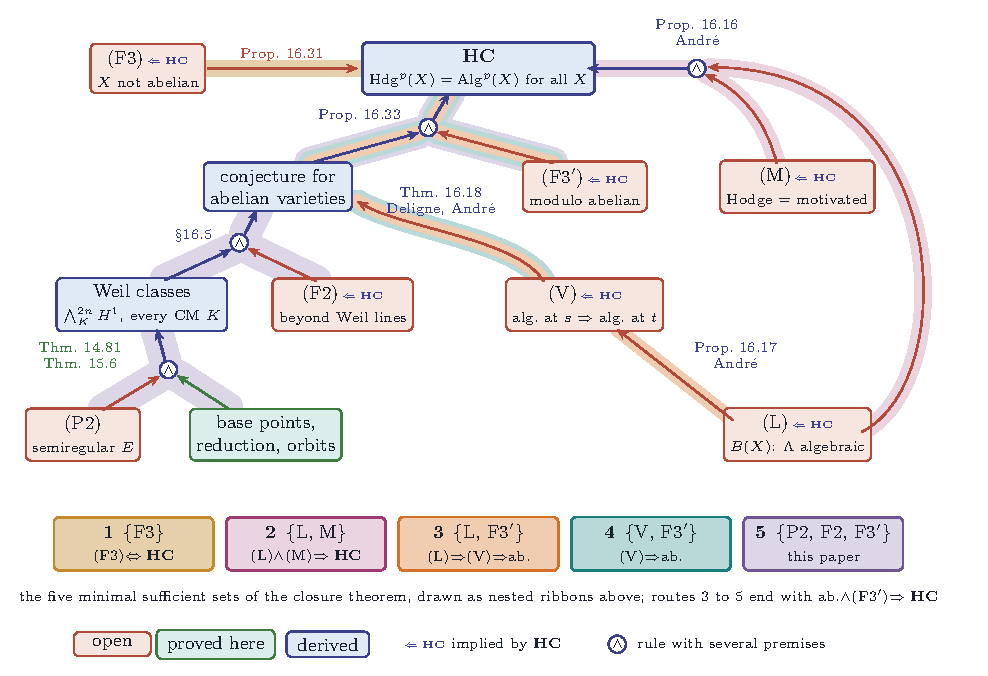
\includegraphics[width=0.92\textwidth]{fig_frontier}
\caption{The rule set of \Cref{setup:rules} with the rules of
\Cref{ssec:bullseye}, drawn as a hypergraph. A rule with several premises is
a junction marked $\wedge$, with arrows from its premises and one arrow to its
conclusion; each rule carries the result that proves it, and the junction
marked \S16.5 is the closure map of \Cref{ssec:closuremap}. Clay marks an
open statement, grass what this paper proves, indigo a derived statement,
and the tag $\Leftarrow\mathbf{HC}$ an open statement that the conjecture
implies: every clay node except (P2). The arrow from (F3) to the conjecture
is \Cref{prop:f3ishc}, and the junction above the conjecture for abelian
varieties is \Cref{prop:f3prime}(i). The five minimal sufficient sets of
\Cref{thm:closure}(ii) are drawn as nested ribbons under the arrows they
use, widest first, and listed in the cards below: (F3) alone; (L) with (M);
(L) through (V) with \textup{(F3$'$)}; (V) with \textup{(F3$'$)}; and, on
the left, (P2) with (F2) and \textup{(F3$'$)}. A shared arrow shows the
bands of every route through it. The secant route, which reaches the
imaginary quadratic families only, is drawn in \Cref{fig:closure}.}
\label{fig:frontier}
\end{figure}

\begin{remark}[The target, and what it would take]\label{rem:bullseye}
With the rules of \Cref{ssec:bullseye}, \Cref{prop:f3ishc} and
\Cref{prop:f3prime} in place, \Cref{thm:closure} changes the reading of
\Cref{cor:fourremain} in three ways. First, the route through this paper is
a route only with (F3) replaced by \textup{(F3$'$)}. As stated, its last
statement (F3) is the conjecture (\Cref{prop:f3ishc}), so (F1) and (F2), and
everything this paper proves about Weil classes, drop out of every minimal
derivation that uses (F3). With \textup{(F3$'$)} in its place the route
$\{\mathrm{P2},\mathrm{F2},\mathrm{F3}'\}$ is minimal, and it is not the
shortest: (F1) and (F2), which between them give the conjecture for abelian
varieties along this route, are replaced on the routes of the literature by
the single statement \textup{(V)}, or by \textup{(L)}, which implies it
(\Cref{thm:vhcab}). Second, every element of every minimal sufficient set
except (P2) is a consequence of the conjecture (\Cref{thm:closure}(vi)), and
two of the sets, $\{\mathrm{F3}\}$ and $\{\mathrm{L},\mathrm{M}\}$, are
each equivalent to it. (P2) is a statement about semiregularity maps, and a
proof of the conjecture need not prove it; in its first form, with a Chern
character that is exactly a Weil class, it is false (\Cref{thm:p2false}), and
the route runs through the corrected form of \Cref{rem:p2prime}. Third, every minimal sufficient set
contains (F3), \textup{(F3$'$)} or \textup{(M)}: the varieties that are not
abelian are reached only through the conjecture for them, which is the whole
conjecture, through the conjecture modulo abelian varieties, which is open
(\Cref{rem:f3primeopen}), or through motivated classes.

So the target at the centre is \textup{(L)}. It lies in two of the five
minimal sets, it gives \textup{(V)} and with it the whole abelian half, the
conjecture implies it, and with \textup{(M)} it is the conjecture. For each
$X$ it asks for one explicit Hodge class on $X\times X$ to be algebraic, the
class inducing $\Lambda$. It is open, as are \textup{(M)}, \textup{(V)}
and \textup{(F3$'$)}, and this paper proves none of them in general:
\Cref{cor:mumfordlefschetz} adds the total spaces of Mumford families to the
known cases of \textup{(L)}, \Cref{prop:f3prime} records the known cases of
\textup{(F3$'$)}, and the routes of the literature use no other theorem of
this paper.
\end{remark}

\subsubsection*{Two of the three are not reductions}

A reader might hope that (F2) and (F3) are reductions in the ordinary sense,
statements to the effect that every Hodge class is carried, by some
correspondence, to a class on a Weil type variety or on an abelian variety,
so that the whole conjecture would follow from the Weil classes alone. Both
hopes are refutable, and we refute them, because a frontier that contains a
false statement is not a frontier.

\begin{proposition}[The Hodge ring is not generated by divisor and Weil
classes]\label{prop:mumfordproduct}
Let $X$ be a complex abelian fourfold whose Hodge group is a $\QQ$-form of an
almost direct product of three copies of $\mathrm{SL}_{2}$, acting on
$V=H^{1}(X,\QQ)$ through the tensor product $V_{1}\otimes V_{2}\otimes V_{3}$
of the three standard representations, with $\End^{0}(X)=\QQ$; such
fourfolds exist and form families of dimension one, by Mumford
\cite{Mum69}, and by \cite[2.5(i)]{MZ99} they are exactly the fourfolds
with $\End^{0}(X)=\QQ$ and Hodge group smaller than $\Sp_{8}$. Then:
\begin{enumerate}[label=\textup{(\roman*)},nosep,leftmargin=2.6em]
\item the Hodge ring of $X$ is generated by the polarisation:
  $\dim_{\QQ}\Hdg^{1}(X)=\dim_{\QQ}\Hdg^{2}(X)=1$;
\item $\dim_{\QQ}\Hdg^{1}(X\times X)=3$ and $\dim_{\QQ}\Hdg^{2}(X\times X)=8$,
  while the products of divisor classes span a subspace of dimension $6$
  in $H^{4}(X\times X,\QQ)$;
\item the two remaining classes lie in $H^{4}(X\times X,\QQ)$ and are Weil
  classes of no CM field acting on $X\times X$, on a quotient of it, or on an
  abelian subvariety of it.
\end{enumerate}
In particular the statement that every Hodge class on an abelian variety
lies in the subring generated by divisor classes and Weil classes of
quotients is false in dimension eight, though true through dimension five
\cite{MZ99}.
\end{proposition}

\begin{proof}
Hodge classes are the invariants of the Hodge group, so
$\Hdg^{k}(Y)\otimes\CC$ is the space of $\Hg(Y)_{\CC}$-invariants in
$\bigwedge^{2k}H^{1}(Y,\CC)$, and $\Hg(X\times X)=\Hg(X)$ acting
diagonally on $V\oplus V$. Over $\CC$ the group is
$\mathrm{SL}_{2}^{3}$ and the weights of $V$ under its maximal torus are the
eight sign vectors $(\pm1,\pm1,\pm1)$. Item (XXXV) of \Cref{sec:verification}
decomposes every $\bigwedge^{k}V$ by peeling highest weights and finds
\begin{gather*}
  \textstyle\bigwedge^{2}V=V(2,2,0)\oplus V(2,0,2)\oplus V(0,2,2)\oplus\mathbf{1},\\
  \textstyle\bigwedge^{4}V=V(2,2,2)\oplus\bigoplus_{\text{cyc}}V(4,0,0)
  \oplus\bigoplus_{\text{cyc}}V(2,2,0)\oplus\mathbf{1},
\end{gather*}
each with one trivial summand, which is (i). For (ii),
$\bigwedge^{4}(V\oplus V)=\bigoplus_{a}\bigwedge^{a}V\otimes\bigwedge^{4-a}V$
and the invariants in $\bigwedge^{a}V\otimes\bigwedge^{4-a}V$ are
$\Hom_{\mathrm{SL}_{2}^{3}}(\bigwedge^{a}V,\bigwedge^{4-a}V)$, since every
summand is self-dual; the counts are $1,1,4,1,1$, total $8$, the $4$ coming
from the four distinct irreducible summands of $\bigwedge^{2}V$. Likewise the
invariants in $\bigwedge^{2}(V\oplus V)$ number $1+1+1=3$. The divisor
classes of $X\times X$ are the three symplectic forms $\psi_{11}$, $\psi_{12}$,
$\psi_{22}$ on $V\oplus V$ built from the polarisation $\psi$ of $V$, and the
same item multiplies them in the exterior algebra of $V\oplus V$ and finds
their six pairwise products linearly independent; it also counts the
$\Sp_{8}$-invariants of $\bigwedge^{4}(V\oplus V)$ by the Weyl character
formula and finds six, so the six products are all the classes a Hodge group
equal to $\Sp_{8}$ would allow. For (iii), the Weil classes of an abelian
variety $Y$ with respect to a CM field $F\subseteq\End^{0}(Y)$ are, by
definition, the classes in $\bigwedge^{2k}_{F}H^{1}(Y,\QQ)\subseteq
H^{2k}(Y,\QQ)$ with $2k=\dim_{F}H^{1}(Y,\QQ)$ (\Cref{setup:cmfield}). A CM
field acting on $X\times X$ lies in $\End^{0}(X\times X)=M_{2}(\QQ)$, so it is
imaginary quadratic, $2k=8$, and its Weil classes lie in $H^{8}$, while the two
classes of (ii) have degree four. Every proper
abelian subvariety and every proper quotient of $X\times X$ is isogenous to
$X$, because $X$ is simple, and $\End^{0}(X)=\QQ$ contains no CM field, so $X$
carries no Weil classes at all. This is the statement of \cite[0.1(iii)]{MZ99}
that the exceptional classes of $X\times X$ are not of Weil type. The last
sentence is (ii) and (iii) together with the theorem of \cite{MZ99} for
dimension at most five.
\end{proof}

\begin{proposition}[No Hodge-theoretic reduction to abelian varieties]
\label{prop:noabeliantype}
Let $Y$ be a very general smooth quintic threefold in $\PP^{4}$, and let
$V=H^{3}(Y,\QQ)$ with its polarised Hodge structure of weight three. Then $V$
is not isomorphic to a subquotient of any Hodge structure of the form
$\bigoplus_{i}T_{i}$, where each $T_{i}$ is obtained from the $H^{1}$ of
finitely many abelian varieties by tensor products, duals and Tate twists. In
particular the Hodge structure $H^{*}(Y,\QQ)$ is not of abelian type, and no
correspondence between $Y$ and an abelian variety, or a product of abelian
varieties, induces an injection of $V$ into the cohomology of the latter.
\end{proposition}

\begin{proof}
Write $\mathrm{MT}(W)$ for the Mumford--Tate group of a rational Hodge
structure $W$ and $\mu_{W}\colon\mathbb{G}_{m}\to\mathrm{MT}(W)_{\CC}$ for
its Hodge cocharacter, acting on $W^{p,q}$ by $z^{p}$. The adjoint action of
$\mu_{W}$ on $\operatorname{Lie}\mathrm{MT}(W)_{\CC}\subseteq\End(W_{\CC})$ has weights
among the differences $p-p'$ of two Hodge indices of $W$.

If $W$ has weight one, these differences lie in $\{-1,0,1\}$. If $W'$ is a
subquotient of a tensor construction $T$ on $W$, then $\mathrm{MT}(W')$ is the
image of $\mathrm{MT}(W)$ acting on $W'$, and $\mu_{W'}$ is the image of
$\mu_{W}$; so $\operatorname{Lie}\mathrm{MT}(W')$ is a quotient of $\operatorname{Lie}\mathrm{MT}(W)$
as a representation of $\mathbb{G}_{m}$ through $\mu$, and its weights are a
subset of $\{-1,0,1\}$. The same holds with $W=\bigoplus H^{1}(A_{i})$.
Hence for every Hodge structure of abelian type the adjoint weights of the
Hodge cocharacter lie in $\{-1,0,1\}$.

For $V=H^{3}(Y,\QQ)$ we show that the adjoint weight $3$ occurs. The
canonical bundle of a quintic threefold is trivial by adjunction, so
$h^{3,0}(Y)=1$; pick $0\ne e\in H^{3,0}$. The intersection form $\psi$ on $V$
is symplectic and pairs $H^{3,0}$ with $H^{0,3}$ perfectly, so the rank one
endomorphism $x\mapsto\psi(x,e)\,e$ of $V_{\CC}$ is nonzero, sends $H^{0,3}$
to $H^{3,0}$ and kills the rest, and lies in $\mathfrak{sp}(V_{\CC},\psi)$
because $\psi(\psi(x,e)e,y)+\psi(x,\psi(y,e)e)
=\psi(x,e)\bigl(\psi(e,y)+\psi(y,e)\bigr)=0$; its adjoint weight is
$3-0=3$. It remains to see that $\mathfrak{sp}(V_{\CC},\psi)\subseteq
\operatorname{Lie}\mathrm{MT}(V)_{\CC}$. Let $S$ be the parameter space of smooth quintic
threefolds, connected and nonsingular, and $\mathbb{V}$ the polarisable
variation of Hodge structure $R^{3}$ of the universal family. The connected
algebraic monodromy group $G^{0}$ of $\mathbb{V}$ contains the connected
monodromy group of any Lefschetz pencil of quintics, that is of hyperplane
sections of the fifth Veronese image of $\PP^{4}$; for a Lefschetz pencil of
odd fibre dimension the image of the monodromy representation on the
$\ell$-adic vanishing cohomology $E\otimes\QQ_{\ell}$ is open in
$\Sp(E\otimes\QQ_{\ell},\psi)$ \cite[Theorem 5.10]{Del74}, so the Zariski
closure of the monodromy group over $\QQ$ is $\Sp(E,\psi)$; here
$E=H^{3}(Y_{t},\QQ)$, the vanishing cohomology being the orthogonal
complement of the image of $H^{3}(\PP^{4},\QQ)=0$. Hence $G^{0}\supseteq
\Sp(V,\psi)$, and $G^{0}\subseteq\Sp(V,\psi)$ since the monodromy preserves
$\psi$. At a very general
point $Y$ the group $G^{0}$ is a normal subgroup of the derived group of
$\mathrm{MT}(V)$ \cite[Theorem 1]{And92}, so $\Sp(V,\psi)\subseteq
\mathrm{MT}(V)^{\mathrm{der}}\subseteq\Sp(V,\psi)$, and the adjoint weight
$3$ occurs in $\operatorname{Lie}\mathrm{MT}(V)$. So $V$ is not of abelian type, and
neither is any Hodge structure containing it as a subquotient, in particular
$H^{*}(Y,\QQ)$. A correspondence inducing an injection of $V$ into the
cohomology of an abelian variety would exhibit $V$ as a sub-Hodge structure
of a Tate twist of that cohomology, which is of abelian type. Item (XXXV)
records the Hodge numbers $(1,101,101,1)$ from the Jacobian ring of the
Fermat quintic, checks the symplectic identity and the weight of the
displayed endomorphism in a four-dimensional model with the same weights, and
lists the adjoint weights that occur.
\end{proof}

\begin{remark}[What the two propositions do to the frontier]
\label{rem:notreductions}
Neither proposition changes \Cref{thm:closure}: the rule set uses (F2) and
(F3) as implications, and an implication whose hypothesis is the conjecture
for one class of Hodge classes and whose conclusion is the conjecture for a
larger class is true whatever the classes are. What does change it is
\Cref{prop:f3ishc}: the varieties of (F3) are not a class disjoint from the
abelian ones but contain them, through products with $\PP^{1}$, so (F3) is
the whole conjecture and not its non-abelian half. What they change is how the
two statements may be read. Before them one could hope that (F2) and (F3) were
structural facts awaiting proof, so that the conjecture would be a theorem
about Weil classes and nothing else; \Cref{prop:mumfordproduct} shows that the
Hodge classes on abelian varieties are not exhausted by divisor and Weil
classes once the dimension reaches eight, and \Cref{prop:noabeliantype} that
the cohomology of a general variety cannot be moved into that of abelian
varieties at all. Each of the two is therefore the Hodge conjecture for a class
of varieties on which the methods of this paper, which are methods about Weil
lines, have no purchase. The product $X\times X$ is itself of
Weil type for every imaginary quadratic $K$, through an embedding
$K\subset M_{2}(\QQ)=\End^{0}(X\times X)$ whose Rosati involution for the
product polarisation is conjugation, with signature $(4,4)$; its Weil classes
lie in $H^{8}$, and its Hodge group is far smaller than $\SU(4,4)$. The two
classes in $H^{4}$ are of a different kind, and they show that even on a
variety of Weil type the Weil line need not be the whole of the exceptional
cohomology once the Hodge group is small. They are the smallest instance of
(F2), and \Cref{ssec:mumford} identifies them and says what one K3 surface
would have to supply for them to be algebraic.
\end{remark}

\begin{figure}[tbp]
\centering
  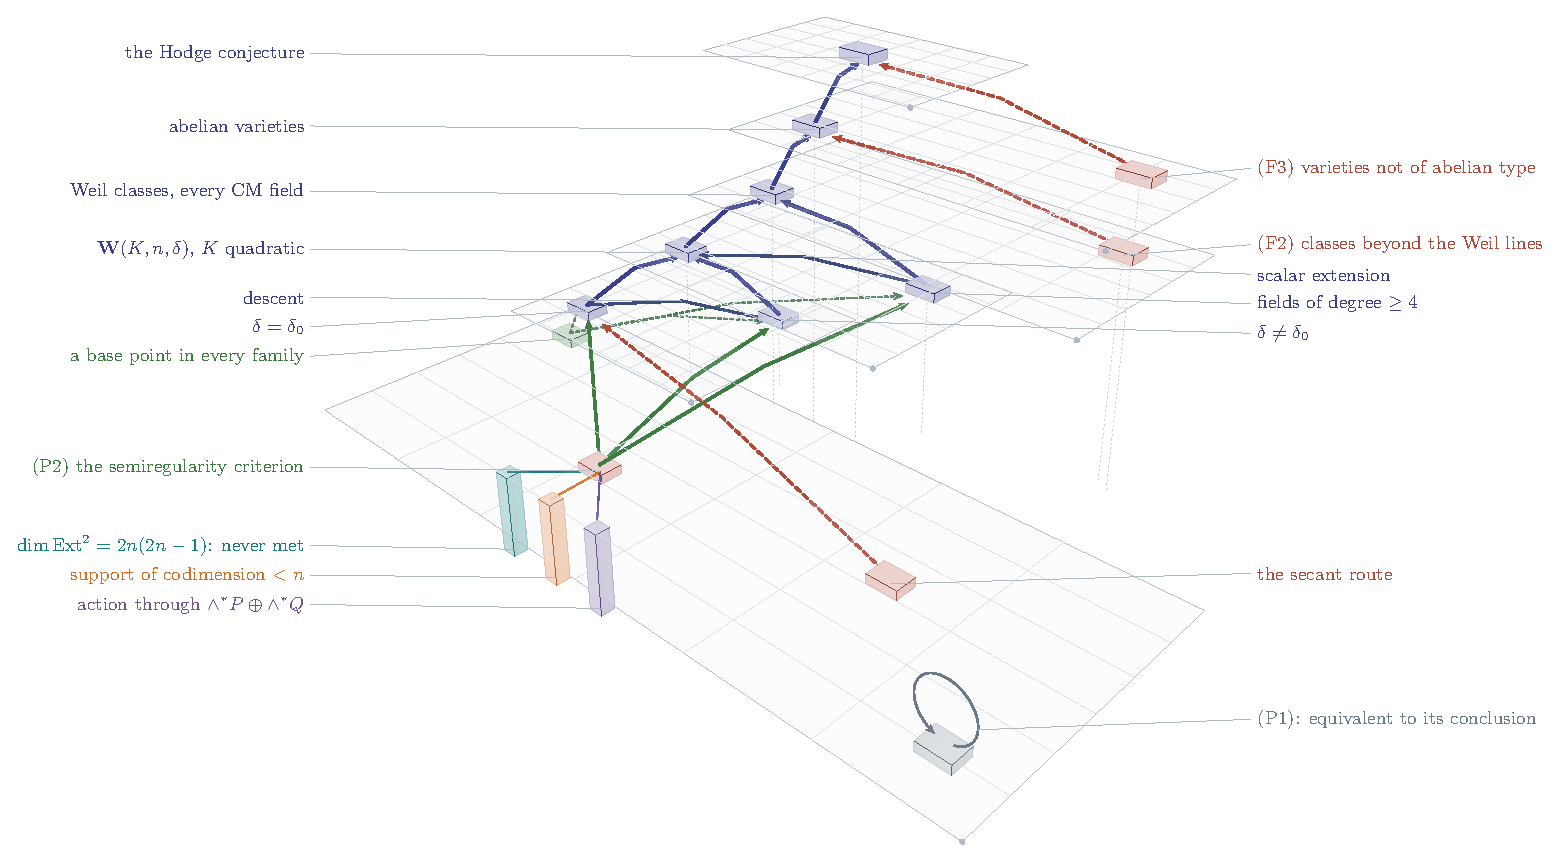
\includegraphics[width=\textwidth]{fig_closure}
\caption{The route of this paper in \Cref{thm:closure}, drawn as a stack of
plates, one per level of the derivation; the other routes of the literature
are drawn in \Cref{fig:frontier}. The spine in indigo runs from the Weil families at the bottom to
the conjecture at the top. The two statements (F2) and (F3) enter in clay from
the right, each at the level where it is needed; (F2) is the conjecture for a
class of Hodge classes that no Weil line reaches, not a reduction, and (F3) is
the whole conjecture (\Cref{prop:f3ishc}), so the route drawn is minimal
only with (F3) replaced by \textup{(F3$'$)} of \Cref{def:f3prime}. From
below,
the propagation statement (P2) in grass reaches the two discriminant cases of
the quadratic fields and the fields of higher degree alike, because
\Cref{thm:everyfamily} and \Cref{thm:cmbasepoint} put a base point in every
family; it is read in the corrected form of \Cref{rem:p2prime}. The two
edges inside the levels are \Cref{prop:descent}: descent from the trivial
discriminant to the others, and scalar extension from the fields of degree at
least four to the quadratic fields; with them (P2) is needed only for the
split families of the fields of higher degree. The three
pillars under the grass node are the results of \Cref{thm:p2numerical},
\Cref{thm:p2support} and \Cref{cor:hhfactor} on the first form, in which the
Chern character is exactly a Weil class; by \Cref{thm:p2false} that form is
never met, so the number on the first pillar is attained by no complex. The
secant route in clay reaches the trivial discriminant, since the member it is
built on is split, and through descent the rest of the quadratic case; it has
no edge to the fields of higher degree. The bounded criterion (P1) is drawn apart, in slate, closed on
itself: it is equivalent to its own conclusion.}
\label{fig:closure}
\end{figure}

\begin{remark}[Where this leaves the secant route]\label{rem:secantplace}
\Cref{thm:closure}(iv) is a statement about the shape of the argument, not
about its difficulty, and we say plainly what it does and does not
mean.

It does not mean the secant route is worthless. It is the only route on which
anything above dimension four has ever been proved, it is the route that
settles $n=2$ at every discriminant and $n=3$ at trivial discriminant, and the
reduction of
\Cref{thm:factor} turns its remaining demand into one identity in the Yoneda
algebra of a sheaf on a fourfold, which is the form in which a demand can be
attacked. What \Cref{cor:cmdichotomy}, \Cref{thm:noci} and
\Cref{thm:nosplit} do to that identity is narrow it to two shapes of
support, neither resolved by sums of line bundles, and, in the smooth shape,
to four discriminants.

What it does mean is that finishing the secant route would not finish the
problem, and would not reduce it either. Through \Cref{prop:descent} it would
give every imaginary quadratic family, the trivial discriminant directly and
the others by descent, which is a great deal; an earlier version of this
remark said that it stops at the trivial discriminant, and that was an
omission of the rule set. It would give nothing over the CM fields of degree
at least four, whose split families need (P2) for themselves, and by
\Cref{prop:descent}(ii) that statement gives the imaginary quadratic fields as
well. So the statement that would have to be proved anyway is the
propagation statement for those split families, and once proved it subsumes
the secant route entirely.

It is tempting to read (C1) and (C2) as what remains for the imaginary
quadratic case, and the computation shows why that reading is wrong: it puts
the demand for a construction where a theorem about propagation belongs.
(C1) and (C2) are demands whose satisfaction would be a considerable
achievement, would settle the Weil classes of every imaginary quadratic field,
and would close nothing that (P2) does not close.
\end{remark}

\subsection{The first classes beyond the Weil lines}\label{ssec:mumford}

Statement (F2) is the Hodge conjecture for the Hodge classes on abelian
varieties that no Weil line reaches, and \Cref{prop:mumfordproduct} exhibits
the first of them: two classes in $H^{4}(X\times X,\QQ)$ for an abelian
fourfold $X$ of Mumford type. None of the constructions of the earlier
sections acts on them. In this subsection we identify them as a real
multiplication on the primitive part of $H^{2}(X)$, and we prove that they
are algebraic as soon as the Kuga--Satake class of one K3 surface of Picard
number thirteen attached to $X$ is algebraic. We do not prove that the
Kuga--Satake class is algebraic, and we know of no proof. What changes is the
kind of question: two classes on an eightfold are traded for one
correspondence of a well-studied type, between a surface and its Kuga--Satake
variety. The field enters through the Clifford relations, which force the
Kuga--Satake map to see all of it.

\begin{setupenv}[Mumford type]\label{setup:mumford}
Let $X$ be as in \Cref{prop:mumfordproduct}, with $V=H^{1}(X,\QQ)$,
polarisation $\psi$ and polarisation class $\theta\in H^{2}(X,\QQ)$, and let
$G=\Hg(X)$. Over $\bar{\QQ}$ the Hodge cocharacter is nontrivial on exactly
one of the three factors of $G$: on $V_{i}$ it has weights $\pm a_{i}/2$ with
$a_{i}\ge0$, and $V$ has only the two weights $\pm\frac12$, so exactly one
$a_{i}$ is nonzero. Because
$\End^{0}(X)=\QQ$ the group $G$ is therefore $\QQ$-simple: the Lie algebra of
a $\QQ$-factor not containing that geometric factor would consist of Hodge
classes in $\End(V)$, that is of endomorphisms of $X$. So $G$ is the image in
$\GL(V)$ of $\Res_{F/\QQ}D^{1}$, where $F$ is a totally real cubic field, $D$
is a quaternion algebra over $F$ split at one real place $\sigma_{3}$ and
definite at the other two, $\sigma_{1}$ and $\sigma_{2}$, with
$\operatorname{Cor}_{F/\QQ}D\cong M_{8}(\QQ)$, and $D^{1}$ is the group of
elements of reduced norm one \cite{Mum69,Gal00}; the kernel is the central
subgroup of triples of signs with product one. Over $\bar{\QQ}$,
$V=V_{1}\otimes V_{2}\otimes V_{3}$, where $V_{i}$ is the standard
representation of $D\otimes_{F,\sigma_{i}}\bar{\QQ}=M_{2}(\bar{\QQ})$; the
Galois group permutes the three factors as it permutes the three embeddings,
and $H^{1,0}(X)=V_{1}\otimes V_{2}\otimes V_{3}^{1,0}$. Put
\[
  T=\operatorname{Lie}G=D^{0},
  \qquad
  q_{\lambda}(x,y)=\Tr_{F/\QQ}\bigl(\lambda\operatorname{trd}(xy)\bigr)
  \quad(\lambda\in F^{\times}),
\]
where $D^{0}$ is the space of quaternions of reduced trace zero, regarded as
a $\QQ$-vector space of dimension nine, and $\operatorname{trd}$ is the
reduced trace. Over $\bar{\QQ}$, $T=T_{1}\oplus T_{2}\oplus T_{3}$ with
$T_{i}=\mathfrak{sl}(V_{i})$, and $a\in F$ acts on $T_{i}$ by $\sigma_{i}(a)$.
Write $m_{a}$ for multiplication by $a$. The space $T\subset\End(V)$ is a
sub-Hodge structure of weight zero.
\end{setupenv}

\begin{proposition}[The two classes are a real multiplication]%
\label{prop:mumfordrm}
In \Cref{setup:mumford}:
\begin{enumerate}[label=\textup{(\roman*)},nosep,leftmargin=2.6em]
\item $H^{2}(X,\QQ)=\QQ\theta\oplus U$, where $U$ is the primitive part, of
  dimension $27$, and over $\bar{\QQ}$
  \[
    U=U_{12}\oplus U_{13}\oplus U_{23},\qquad
    U_{ij}=S^{2}V_{i}\otimes S^{2}V_{j}\otimes{\textstyle\bigwedge^{2}}V_{k},
    \quad \{i,j,k\}=\{1,2,3\},
  \]
  each of dimension nine. The summand $U_{12}$ is of type $(1,1)$, and
  $U_{13}$ and $U_{23}$ have Hodge numbers $(3,3,3)$.
\item The algebra of Hodge endomorphisms of $H^{2}(X,\QQ)$ is $\QQ\times F$,
  acting by scalars on $\QQ\theta$, with $a\in F$ acting on $U_{ij}$ by
  $\sigma_{k}(a)$. Through Poincar\'e duality and the Lefschetz isomorphism
  $\theta^{2}\colon H^{2}\to H^{6}$ this algebra is the space of Hodge classes
  in the K\"unneth component $H^{2}(X)\otimes H^{2}(X)$ of
  $H^{4}(X\times X,\QQ)$; the subalgebra $\QQ\times\QQ$ is spanned by the
  products of divisor classes that lie there, and the two classes of
  \Cref{prop:mumfordproduct}(ii) may be taken to be the elements of $F$ of
  trace zero.
\item $T(-1)$ is a Hodge structure of K3 type with Hodge numbers $(1,7,1)$,
  and its Hodge endomorphisms are the $m_{a}$, $a\in F$. The $G$-invariant
  symmetric forms on $T$ are the $q_{\lambda}$, and $q_{\lambda}$ polarises
  $T(-1)$ if and only if $\lambda$ is totally positive.
\end{enumerate}
\end{proposition}

\begin{proof}
(i) is the decomposition of $\bigwedge^{2}(V_{1}\otimes V_{2}\otimes V_{3})$
in the proof of \Cref{prop:mumfordproduct}, where $U_{ij}$ appears as the
summand of highest weight $2$ on the $i$-th and $j$-th factors. The Hodge
cocharacter acts trivially on $V_{1}$ and $V_{2}$ and splits
$V_{3}=V_{3}^{1,0}\oplus V_{3}^{0,1}$, so $\bigwedge^{2}V_{3}$ has type
$(1,1)$ and $S^{2}V_{3}$ has one dimension of each of the types $(2,0)$,
$(1,1)$, $(0,2)$.

(ii) A Hodge endomorphism commutes with the Mumford--Tate group $G\cdot\mathbb{G}_{m}$, and
$\mathbb{G}_{m}$ acts on $H^{2}$ by scalars, so the Hodge endomorphisms are
the $G$-endomorphisms. Over $\bar{\QQ}$ the four summands $\QQ\theta$,
$U_{12}$, $U_{13}$, $U_{23}$ are irreducible and pairwise non-isomorphic, so
the $G$-endomorphisms are the combinations of the four projections. The
Galois group fixes the projection onto $\QQ\theta$ and permutes the other
three as it permutes the indices $k$, that is as it permutes the embeddings of
$F$. An endomorphism acting on $U_{ij}$ by $\sigma_{k}(a)$ is therefore
Galois invariant, hence rational, and these exhaust the rational points,
which are $\QQ\times F$. Poincar\'e duality identifies $\End H^{2}(X,\QQ)$
with $H^{6}(X)\otimes H^{2}(X)$, and $\theta^{2}\otimes1$ carries
$H^{2}\otimes H^{2}$ onto it; both are given by algebraic classes, and on an
abelian variety so is the inverse of the Lefschetz isomorphism
\cite[\S2]{Kle68}. The products of divisor classes in $H^{2}\otimes H^{2}$
are $\psi_{11}\psi_{22}$ and $\psi_{12}^{2}$ in the notation of the proof of
\Cref{prop:mumfordproduct}. They are invariant under the whole of
$\Sp(V,\psi)$, whose endomorphisms of $H^{2}=\QQ\theta\oplus U$ are spanned
by the identity and the projection onto $\QQ\theta$, and they are linearly
independent by item (XXXV); so they span $\QQ\times\QQ$, and any complement of
$\QQ\times\QQ$ in $\QQ\times F$ may serve as the two remaining classes.

(iii) The adjoint action of the Hodge cocharacter is trivial on $T_{1}$ and
$T_{2}$ and has weights $-1$, $0$, $1$ on $T_{3}$, so $T$ has Hodge numbers
$(1,7,1)$ in the types $(-1,1)$, $(0,0)$, $(1,-1)$, and $T(-1)$ is of K3
type. Its Hodge endomorphisms are again the $G$-endomorphisms, and the
argument of (ii), applied to the three pairwise non-isomorphic summands
$T_{i}$, gives $F$ acting by multiplication. On each $T_{i}$ the invariant
symmetric forms are the multiples of $\operatorname{tr}(xy)$, and
$\operatorname{tr}(x_{i}y_{i})=\sigma_{i}(\operatorname{trd}(xy))$ for
$x,y\in D^{0}$, so the Galois-invariant ones are the $q_{\lambda}$. At
$\sigma_{1}$ and $\sigma_{2}$ the algebra $D\otimes\RR$ is Hamilton's
quaternions, $T_{i}$ is of type $(1,1)$, and $\operatorname{trd}(x^{2})=-2\operatorname{nrd}(x)$ is
negative on nonzero pure quaternions. At $\sigma_{3}$ the form
$\operatorname{tr}(xy)$ on $\mathfrak{sl}_{2}(\RR)$ is negative on the line of
type $(1,1)$, the Lie algebra of the rotations fixed by the Hodge
cocharacter, and positive on its orthogonal complement, the real points of
the types $(2,0)$ and $(0,2)$. The Hodge--Riemann relations for a structure
of K3 type ask for exactly these signs after multiplication by
$\sigma_{i}(\lambda)$, so $q_{\lambda}$ polarises $T(-1)$ precisely when every
$\sigma_{i}(\lambda)$ is positive. Item (XLI) of \Cref{sec:verification}
computes the four projections from the Casimir operators of the three factors
on an explicit model and checks (i) and the Hodge numbers.
\end{proof}

The two classes are thus the endomorphisms of $U$ given by the elements of
$F$ of trace zero. A Hodge structure of K3 type with the same field sits
beside them, and the next lemma connects the two.

\begin{lemma}[The product map]\label{lem:mumfordmu}
For $x,y\in T$ let $\mu(x\otimes y)\in H^{2}(X,\QQ)$ be the class that
corresponds under $\psi$ to the alternating form
$(v,w)\mapsto\psi(xv,yw)+\psi(yv,xw)$ on $V$. Then $\mu$ is a $G$-equivariant
map $T\otimes T\to H^{2}(X,\QQ)$, and:
\begin{enumerate}[label=\textup{(\roman*)},nosep,leftmargin=2.6em]
\item for $i\ne j$ it restricts to an isomorphism $T_{i}\otimes T_{j}\to
  U_{ij}$, and it carries $T_{i}\otimes T_{i}$ onto $\QQ\theta$;
\item for $e,\lambda\in F^{\times}$ put $\mu_{e}=\mu\circ(m_{e}\otimes m_{e})$
  and let $\mu_{e}^{\dagger}$ be its adjoint for the form
  $q_{\lambda}\otimes q_{\lambda}$ on $T\otimes T$ and the Lefschetz pairing
  $B(\alpha,\beta)=\int_{X}\alpha\beta\,\theta^{2}$ on $H^{2}(X,\QQ)$. Then
  $\mu_{e}\mu_{e}^{\dagger}$ preserves $\QQ\theta$ and acts on $U$ as the
  element
  \[
    \nu\,\Nm_{F/\QQ}(g)\,g^{-1}\in F,\qquad g=e^{2}/\lambda,
  \]
  where $\nu$ is a nonzero rational number independent of $e$ and $\lambda$.
\end{enumerate}
\end{lemma}

\begin{proof}
Equivariance is clear, since $\mu$ is built from $\psi$ and the action of
$\End(V)$ on $V$. An element $x\in T_{i}$ acts on $V$ through the $i$-th factor
and lies in the symplectic Lie algebra of $\psi=\epsilon_{1}\otimes
\epsilon_{2}\otimes\epsilon_{3}$, so $\psi(xv,yw)=-\psi(v,xyw)$ and
$\mu(x\otimes y)$ is the form $-\psi(v,(xy+yx)w)$. If $x\in T_{i}$ and
$y\in T_{j}$ with $i\ne j$, then $xy=yx$ acts as $x\otimes y$ on
$V_{i}\otimes V_{j}$, and the form is $-2$ times the product of
$\epsilon_{i}(\cdot,x\,\cdot)$, $\epsilon_{j}(\cdot,y\,\cdot)$ and
$\epsilon_{k}$; the first two are symmetric because $x$ and $y$ lie in
$\mathfrak{sp}(\epsilon)=\mathfrak{sl}_{2}$, and $x\mapsto\epsilon(\cdot,x\,\cdot)$
is an isomorphism $\mathfrak{sl}_{2}\to S^{2}V^{\vee}$, so $\mu$ maps
$T_{i}\otimes T_{j}$ isomorphically onto $U_{ij}$. If $i=j$, then
$xy+yx=\operatorname{tr}(xy)$ on $V_{i}$, because $x$ and $y$ are trace-free
$2\times2$ matrices, and $\mu(x\otimes y)=-\operatorname{tr}(xy)\,\theta$.

For (ii), $m_{e}$ is self-adjoint for $q_{\lambda}$, and the adjoint of a
map out of $(T\otimes T,q_{\lambda}\otimes q_{\lambda})$ is
$(m_{\lambda}\otimes m_{\lambda})^{-1}$ times its adjoint for
$q_{1}\otimes q_{1}$, so
$\mu_{e}\mu_{e}^{\dagger}=\mu\,(m_{g}\otimes m_{g})\,\mu^{\dagger_{1}}$ with
$\mu^{\dagger_{1}}$ the adjoint for $q_{1}\otimes q_{1}$. This map is
$G$-equivariant, so it preserves $\QQ\theta$ and each $U_{ij}$, and
$\mu^{\dagger_{1}}$ carries $U_{ij}$ into
$(T_{i}\otimes T_{j})\oplus(T_{j}\otimes T_{i})$, on which $m_{g}\otimes m_{g}$
is multiplication by $\sigma_{i}(g)\sigma_{j}(g)=\Nm(g)/\sigma_{k}(g)$. Hence
$\mu_{e}\mu_{e}^{\dagger}$ is $\Nm(g)\sigma_{k}(g)^{-1}$ times
$\mu\mu^{\dagger_{1}}$ on $U_{ij}$. Item (XLI) computes $\mu\mu^{\dagger_{1}}$
on the split model and finds one and the same nonzero rational number $\nu$
on the three summands $U_{ij}$; it also checks the formula for
$\mu_{e}\mu_{e}^{\dagger}$ directly for several values of the conjugates of
$e$ and $\lambda$. By \Cref{prop:mumfordrm}(ii) an endomorphism of $U$ acting
on $U_{ij}$ by $\nu\Nm(g)/\sigma_{k}(g)$ is the element $\nu\Nm(g)g^{-1}$ of
$F$.
\end{proof}

By the Kuga--Satake class of a projective K3 surface $S$ we mean the Hodge
class on $S\times\mathrm{KS}(S)\times\mathrm{KS}(S)$ that induces the embedding
of \Cref{prop:ksembed} for $T(S)_{\QQ}$; its algebraicity is the Kuga--Satake
Hodge conjecture for $S$ of \Cref{rem:kstransport}.

\begin{theorem}[One K3 surface for the two classes]\label{thm:mumfordks}
In \Cref{setup:mumford}, let $\lambda\in F$ be totally positive.
\begin{enumerate}[label=\textup{(\roman*)},nosep,leftmargin=2.6em]
\item There is a projective K3 surface $S_{\lambda}$ of Picard number
  thirteen and an isomorphism of Hodge structures
  $T(S_{\lambda})_{\QQ}\cong T(-1)$ carrying the intersection form to
  $q_{\lambda}$. Its Kuga--Satake variety is isogenous to $X^{32}$.
\item If the Kuga--Satake class of $S_{\lambda}$ is algebraic, then the real
  multiplication by $F$ on $T(S_{\lambda})$ is induced by algebraic cycles on
  $S_{\lambda}\times S_{\lambda}$, and every Hodge class in
  $H^{4}(X\times X,\QQ)$ is algebraic; in particular the two classes of
  \Cref{prop:mumfordproduct}(ii) are algebraic.
\end{enumerate}
\end{theorem}

\begin{proof}
(i) The quadratic space $(T,q_{\lambda})$ has dimension nine and signature
$(2,7)$ by \Cref{prop:mumfordrm}(iii), and $H^{2}$ of a K3 surface with its
intersection form has dimension $22$ and signature $(3,19)$. Over $\QQ_{p}$
a nondegenerate quadratic space embeds isometrically in every nondegenerate
space of dimension at least three larger, and over $\RR$ the signatures
allow it, so by the Hasse--Minkowski theorem for representations of forms by
forms \cite[\S\S63, 66]{OMe00} there is an isometric embedding of
$(T,q_{\lambda})$ into $\Lambda_{\QQ}$, where $\Lambda$ is the K3 lattice.
The line $\ell=T(-1)^{2,0}\subset T_{\CC}\subset\Lambda_{\CC}$ satisfies
$(\ell,\ell)=0$ and $(\sigma,\bar{\sigma})>0$ for $0\ne\sigma\in\ell$, so by the
surjectivity of the period map there is a K3 surface $S_{\lambda}$ with a
marking $H^{2}(S_{\lambda},\ZZ)\cong\Lambda$ that carries
$H^{2,0}(S_{\lambda})$ to $\ell$ \cite[Chs.~6--7]{Huy16}. A rational class
is of type $(1,1)$ exactly when it is orthogonal to $\ell$, and its component
in $T$ is then a rational class of type $(1,1)$ in $T(-1)$, that is a
$G$-invariant vector of $T=\operatorname{Lie}G$; there is none, since $G$ is
semisimple. So $\NS(S_{\lambda})_{\QQ}=T^{\perp}$, of dimension $13$ and
signature $(1,12)$, and $T(S_{\lambda})_{\QQ}=T$ with the form $q_{\lambda}$.
A class of positive square in $\NS(S_{\lambda})$ makes $S_{\lambda}$
projective \cite[Ch.~8]{Huy16}.

For the Kuga--Satake variety, note first that over $\bar{\QQ}$ the space $T$
is the orthogonal sum of the three ternary spaces $T_{i}$, so $C(T)$ is the
graded tensor product of the $C(T_{i})$. Scaling a ternary form does not
change its even Clifford algebra, so $D^{1}$ is the spin group of
$(D^{0},\lambda\operatorname{trd})$ for every $\lambda$, and
$\Res_{F/\QQ}D^{1}$ maps to $\mathrm{Spin}(T,q_{\lambda})$ by multiplication
in the Clifford algebra, with the same kernel as its map to $\GL(V)$, so that
$G$ is a subgroup of $\mathrm{Spin}(T,q_{\lambda})$; as a representation of the $i$-th factor,
$C(T_{i})$ is four copies of $V_{i}$. Hence $C^{+}(T)$ is $V^{\oplus32}$ as a
representation of $G$ over $\bar{\QQ}$, and over $\QQ$ as well, because $V$ is
absolutely irreducible. The Hodge structures on $C^{+}(T)=H^{1}(\mathrm{KS}(S_{\lambda}),\QQ)$
and on $V^{\oplus32}=H^{1}(X^{32},\QQ)$ are both given by lifts of weight one of
the same homomorphism $\mathbb{S}\to\MT(T)_{\RR}$ through $G\cdot\mathbb{G}_{m}$, and
two such lifts coincide.\footnote{They differ by a homomorphism from the
anisotropic torus $\mathbb{S}/\mathbb{G}_{m}$ to the centre of
$G\cdot\mathbb{G}_{m}$, whose identity component is $\mathbb{G}_{m}$, and
such a homomorphism is trivial.} So
$H^{1}(\mathrm{KS}(S_{\lambda}),\QQ)\cong H^{1}(X^{32},\QQ)$ as Hodge
structures, and $\mathrm{KS}(S_{\lambda})$ is isogenous to $X^{32}$. For the
form Galluzzi uses this is her theorem \cite{Gal00}, and van Geemen proves the
corresponding splitting for every K3 surface with real multiplication
\cite{vG08}.

(ii) Write $S=S_{\lambda}$ and $A=\mathrm{KS}(S)$, and let $Z_{S}$ be an
algebraic cycle on $S\times A\times A$ inducing the Kuga--Satake embedding
$T(S)\to\End H^{1}(A)$. Composing $Z_{S}$ with the graph of an isogeny
$A\to X^{32}$ and with the graphs of the inclusions and projections of the
factors of $X^{32}$ gives algebraic cycles on $S\times X\times X$ inducing the
$32^{2}$ block components of the embedding, which are morphisms of Hodge
structures $T(S)\to\End(V)$, up to a Tate twist; both lie in the tensor
category generated by $H^{1}(X)$, so the blocks are equivariant for
$\MT(X)=G\cdot\mathbb{G}_{m}$. Over $\bar{\QQ}$,
$\End(V)=S^{2}V\oplus\bigwedge^{2}V$, and $T_{i}\cong S^{2}V_{i}$ occurs once
in $S^{2}V$, as $S^{2}V_{i}\otimes\bigwedge^{2}V_{j}\otimes\bigwedge^{2}V_{k}$,
and not at all in $\bigwedge^{2}V$. So each block takes values in $T$, and
through the identification of (i) it is a $G$-endomorphism of $T$, that is
$m_{e_{ab}}$ for some $e_{ab}\in F$ by \Cref{prop:mumfordrm}(iii). Over
$\bar{\QQ}$ the embedding is therefore $v\mapsto v\otimes N_{i}$ on $T_{i}$,
acting on $H^{1}(A)=V\otimes\QQ^{32}$, with
$N_{i}=(\sigma_{i}(e_{ab}))_{a,b}$. The embedding $\Psi$ of
\Cref{prop:ksembed} satisfies the Clifford relation
$\Psi(v)\Psi(w)+\Psi(w)\Psi(v)=2q_{\lambda}(v_{0},v_{0})\,q_{\lambda}(v,w)$,
because
$\Psi(v)\Psi(w)x=vwx\,v_{0}^{2}$. Take nonzero $v\in T_{i}$ and
$w\in T_{j}$ with $i\ne j$. As endomorphisms of $V$ they commute and $vw\ne0$,
so the left side is $vw\otimes(N_{i}N_{j}+N_{j}N_{i})$, while the right side
is zero because $T_{i}$ and $T_{j}$ are orthogonal; hence $N_{i}$ and $N_{j}$
anticommute. For $v\in T_{i}$ with $q_{\lambda}(v,v)\ne0$ the relation reads
$v^{2}\otimes N_{i}^{2}=q_{\lambda}(v_{0},v_{0})\,q_{\lambda}(v,v)$, and $v^{2}$
is a nonzero scalar on $V_{i}$, so $N_{i}^{2}$ is a nonzero scalar. Three pairwise
anticommuting invertible matrices are linearly independent: multiplying a
relation $\sum_{i}c_{i}N_{i}=0$ by $N_{j}$ on either side and adding gives
$2c_{j}N_{j}^{2}=0$. If the $e_{ab}$ spanned a subspace of $F$ of dimension at
most two, the $N_{i}$ would lie in the span of at most two rational matrices;
so the $e_{ab}$ span $F$, and two of them, $e$ and $e'$, are not rational
multiples of each other. Then $(e/e')^{2}$ is irrational, since a cubic field
contains no irrational element with rational square, so $e^{2}/\lambda$ and
$e'^{2}/\lambda$ are not both rational. Fix a block $\kappa=m_{e}$ with
$e^{2}/\lambda\notin\QQ$, induced by a cycle $\Gamma$. Item (XLI) builds the
Clifford algebra of the split model and checks that $\Psi$ has this shape,
with three anticommuting $N_{i}$.

The real multiplication first. The trace form $(a,b)\mapsto\operatorname{tr}(ab)$ on
$\End(V)$ is induced by an algebraic class: for correspondences $a,b$ on $X$
the Lefschetz trace formula gives
$\operatorname{tr}(a_{*}b_{*}\mid H^{1})=-\deg\bigl((a\circ b\circ\pi_{1})\cdot\Delta_{X}\bigr)$,
where $\pi_{1}$ is the K\"unneth projector onto $H^{1}$, algebraic on an
abelian variety \cite[\S2]{Kle68}. So the adjoint $\kappa^{\dagger}$ of
$\kappa$, for this form and the intersection form on $S$, is induced by a
cycle built from the transpose of $\Gamma$, $\pi_{1}$ and $\Delta_{X}$, and
$\kappa^{\dagger}\kappa$ is an algebraic endomorphism of $T(S)$. An element $x$ of $T_{i}$ acts on the
eight-dimensional space $V$ through a two-dimensional factor, with
multiplicity four, so $\operatorname{tr}_{V}(xy)=4\Tr_{F/\QQ}\operatorname{trd}(xy)$, and
\[
  q_{\lambda}(\kappa^{\dagger}\kappa x,y)
  =\operatorname{tr}_{V}(ex\cdot ey)
  =4\Tr_{F/\QQ}\bigl(e^{2}\operatorname{trd}(xy)\bigr)
  =q_{\lambda}\bigl(4e^{2}\lambda^{-1}x,y\bigr),
\]
that is $\kappa^{\dagger}\kappa=m_{4e^{2}/\lambda}$. By the choice of $e$ this
element is irrational, so it generates the cubic field $F$ and every $m_{a}$
is a polynomial in $\kappa^{\dagger}\kappa$. Composing with the projector of
$H^{2}(S)$ onto $T(S)$, which is algebraic because it is the diagonal minus
$[\mathrm{pt}\times S]$, $[S\times\mathrm{pt}]$ and $\sum_{r}d_{r}\times d_{r}^{\vee}$
over dual bases of $\NS(S)_{\QQ}$, gives algebraic cycles on $S\times S$
inducing the real multiplication.

The classes on $X\times X$ next. The map $\mu_{\kappa}=\mu\circ(\kappa\otimes\kappa)$
from $T(S)\otimes T(S)$ to $H^{2}(X,\QQ)$ is induced by an algebraic cycle on
$S\times S\times X$, obtained from $\Gamma\times\Gamma$, the divisor
$m^{*}\theta-p_{1}^{*}\theta-p_{2}^{*}\theta$ on $X\times X$, whose class is
$\psi$ in $H^{1}\otimes H^{1}$, and the diagonal of $X$ by pull-back,
push-forward and intersection, because $\mu$ uses nothing but $\psi$ and the
composition of endomorphisms of $V$.
The form $q_{\lambda}\otimes q_{\lambda}$ is the intersection form of
$S\times S$ on $T(S)\otimes T(S)$ and $B$ is the intersection form of $X$
twisted by $\theta^{2}$, so the adjoint $\mu_{\kappa}^{\dagger}$ is induced by
cup product with $\theta^{2}$ followed by the transposed cycle, and
$E=\mu_{\kappa}\mu_{\kappa}^{\dagger}$ is an algebraic endomorphism of
$H^{2}(X,\QQ)$. Since $\kappa=m_{e}$, \Cref{lem:mumfordmu}(ii) says that $E$
preserves $\QQ\theta$ and acts on $U$ as $\nu\Nm(g)g^{-1}$ with
$g=e^{2}/\lambda$, and this element of $F$ is not rational, since $g$ is
not. The projection $\pi_{\theta}$ onto $\QQ\theta$ is algebraic, being
given by the class $\theta\times\theta$ suitably normalised, so the algebraic
Hodge endomorphisms of $H^{2}(X,\QQ)$ contain $1$, $\pi_{\theta}$ and
$E(1-\pi_{\theta})$, which generate $\QQ\times F$, that is all of them by
\Cref{prop:mumfordrm}(ii). By the same part every Hodge class in
$H^{2}(X)\otimes H^{2}(X)$ is then algebraic. The Hodge classes of
$H^{4}(X\times X,\QQ)$ in the other K\"unneth components number one in each
of $H^{a}\otimes H^{4-a}$, $a\ne2$, by the count in the proof of
\Cref{prop:mumfordproduct}, and are products of divisor classes.
\end{proof}

\begin{figure}[tbp]
\centering
  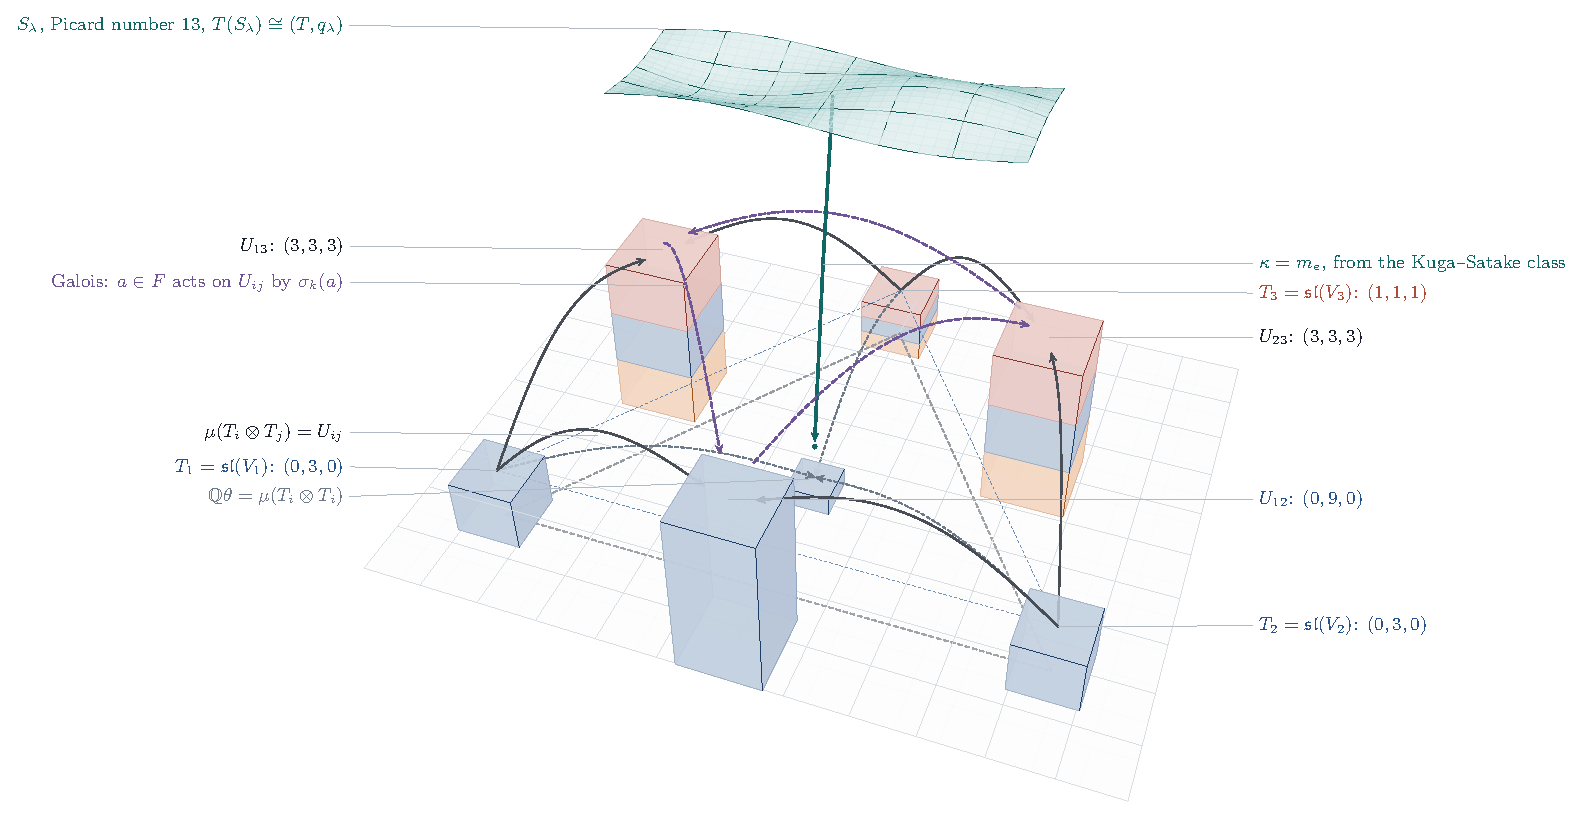
\includegraphics[width=\textwidth]{fig_mumford}
\caption{\Cref{prop:mumfordrm} and \Cref{lem:mumfordmu}, drawn over the
triangle of the three factors of the Hodge group; every height is a
dimension. At the corners stand the summands $T_{i}=\mathfrak{sl}(V_{i})$ of
$T=\operatorname{Lie}G$, banded by Hodge type after the Tate twist $T(-1)$: blue for
$(1,1)$, clay for $(2,0)$ and amber for $(0,2)$, so that only $T_{3}$ carries
the K3 type. On the edges stand the three summands $U_{ij}$ of the primitive
part of $H^{2}(X)$, of dimension nine, $U_{12}$ of pure type $(1,1)$ and the
other two in three bands of three; in the middle is the line of $\theta$. The
solid arcs are the product map $\mu$, which carries $T_{i}\otimes T_{j}$ onto
$U_{ij}$, and the dashed ones carry $T_{i}\otimes T_{i}$ to $\QQ\theta$. The
violet arcs are the Galois group permuting the $U_{ij}$ as it permutes the
embeddings of $F$, which is why the two exceptional classes may be taken to be
the trace-zero part of a cubic field. Above, the K3 surface $S_{\lambda}$ of
\Cref{thm:mumfordks}, whose Kuga--Satake class, if algebraic, comes down to
$T$ as the map $\kappa=m_{e}$.}
\label{fig:mumford}
\end{figure}

\begin{remark}[What is known about the Kuga--Satake class]
\label{rem:mumfordks}
The Kuga--Satake class of $S_{\lambda}$ is not known to be algebraic, and
\Cref{thm:mumfordks} does not make it so. The known cases of the Kuga--Satake
Hodge conjecture lie elsewhere. They include the K3 surfaces of Picard number
at least seventeen, which Morrison relates to abelian surfaces \cite{Mor84},
and the double planes branched along six lines, of Picard number
at least sixteen, settled by Paranjape's cycle; see \cite{vG00}. Floccari
proves the conjecture for the K3 surfaces attached to projective sixfolds of
generalised Kummer type \cite{Flo24}, whose transcendental lattices embed,
after scaling, in the rational second cohomology of such a sixfold, of rank
seven and signature $(3,4)$; their transcendental rank is therefore at most
six, and the surfaces $S_{\lambda}$ have transcendental rank nine.
Schlickewei made the real multiplication algebraic on those double planes
that have it, necessarily by a field of degree at most two, from Paranjape's
cycle and van Geemen's description of their Kuga--Satake varieties
\cite{Sch10,vG08}, and Varesco showed that when the Kuga--Satake Hodge
conjecture holds for two hyperk\"ahler varieties, every Hodge similarity
between their transcendental lattices is algebraic up to the Lefschetz
isomorphism \cite{Var23}, which reaches a quadratic field through its square
root. A cubic field contains no irrational element with rational square, so
none of its elements acts as a similarity; the element
$\kappa^{\dagger}\kappa=m_{4e^{2}/\lambda}$ in the proof takes the place that
the similarities occupy there, and the Clifford relations are what make it
irrational. Buskin's theorem that rational Hodge isometries between K3
surfaces are algebraic \cite{Bus19} does not give the real multiplication
either. A Hodge isometry of $T(S_{\lambda})$ is a Hodge endomorphism, hence
some $m_{a}$ by \Cref{prop:mumfordrm}(iii), and it is an isometry only when
$a^{2}=1$. For $b\in F^{\times}$ the theorem does give algebraic cycles between
$S_{\lambda}$ and $S_{\lambda b^{-2}}$ that realise $m_{b}$, but every composite
of them that returns to $S_{\lambda}$ is again a Hodge isometry of
$T(S_{\lambda})$, so it multiplies by an element of square one.

The surfaces $S_{\lambda}$ include those of Zhu, who computes the integral
structure that the fourfold induces on $T$ and studies the K3 surfaces of
Picard number thirteen that carry it \cite{Zhu18}; its form is the
corestriction of the reduced norm of $D^{0}$, which up to sign is
$\frac12q_{1}$.
\Cref{thm:mumfordks} applies to them as it stands, because the irrationality
of $e^{2}/\lambda$ comes from the anticommuting blocks and not from $\lambda$.
The closest explicit families are those of van Geemen and Sch\"utt, with
real multiplication by the cyclic cubic fields $\QQ(\zeta_{7}+\zeta_{7}^{-1})$
and $\QQ(\zeta_{9}+\zeta_{9}^{-1})$ and Picard numbers four and ten, on which
the real multiplication is induced by explicit algebraic cycles
\cite[Theorem~1.2 and Section~4.8]{vGS25}; their Picard numbers are not
thirteen, and the Kuga--Satake class, which \Cref{thm:mumfordks} needs and
algebraic real multiplication does not supply, is not treated there.
The first case of (F2) is therefore implied by one instance of the
Kuga--Satake Hodge conjecture, for one K3 surface of Picard number thirteen,
and the argument stops there.
\end{remark}

\subsection{The Mumford target: rigidity, a numerical criterion, and the
bypasses}\label{ssec:mumfordrigid}

The first case of (F2) is now a propagation problem along one compact
Shimura curve: the exceptional classes are algebraic at every CM point
(\Cref{thm:mumfordcm}), and on every member exactly when $B(W\times_{C}W)$
holds (\Cref{cor:mumfordequiv}). This subsection asks whether the
propagation can be obtained without passing through the Lefschetz standard
conjecture, by one of the mechanisms that have closed other cases of the
Hodge conjecture: a degeneration, a deformation into a larger family on which
the class stays of Hodge type, a specialisation to special points, or
semiregularity. It proves that the first two cannot work, that the third
works exactly when the representing cycles have bounded degree, and it
reduces the fourth to one dimension count at one CM point. It does not prove
the classes algebraic at a very general point.

\begin{setupenv}[The classes $\omega_{a}$]\label{setup:omegaa}
Keep \Cref{setup:mumford} and let $W\to C$ be a family as in
\Cref{cor:mumfordlefschetz}, with fibres $X_{t}$. Over $\bar{\QQ}$ let
$\pi_{0},\pi_{12},\pi_{13},\pi_{23}\in H^{2}(X)\otimes H^{2}(X)\subset
H^{4}(X\times X)$ be the classes that correspond, under the isomorphism
$H^{2}\otimes H^{2}\cong\End H^{2}$ given by the form ${\textstyle\bigwedge^{2}}\psi$
on $H^{2}(X)={\textstyle\bigwedge^{2}}V^{\vee}$, to the projections onto $\QQ\theta$,
$U_{12}$, $U_{13}$ and $U_{23}$ of \Cref{prop:mumfordrm}(i), and for
$a=(a_{0},a_{1},a_{2},a_{3})$ put
\[
  \omega_{a}=a_{0}\pi_{0}+a_{1}\pi_{12}+a_{2}\pi_{13}+a_{3}\pi_{23},
  \qquad L_{0}(a)=a_{0}+a_{1}+a_{2}+a_{3}.
\]
The four tensors are invariant under $G$ and under the exchange $\tau$ of the
two factors of $X\times X$, because ${\textstyle\bigwedge^{2}}\psi$ is symmetric; so each
$\omega_{a}$ is a flat section over $C$ of Hodge type at every point. The
argument of \Cref{prop:mumfordrm}(ii) shows that the rational ones are those
with $a_{0}\in\QQ$ and $(a_{1},a_{2},a_{3})=(\sigma_{3}(\alpha),
\sigma_{2}(\alpha),\sigma_{1}(\alpha))$ for some $\alpha\in F$; we call such a
class \emph{exceptional} when $\alpha\notin\QQ$. The products of divisor
classes in $H^{2}\otimes H^{2}$ are the rational $\omega_{a}$ with
$\alpha\in\QQ$, and $\pi_{0}$ is a multiple of
$\mathrm{pr}_{1}^{*}\theta\cup\mathrm{pr}_{2}^{*}\theta$; so adding a rational
multiple of $\pi_{0}$ to an exceptional class changes $L_{0}$ and not the
question of algebraicity. For $c\in C$ write $Y=X_{c}\times X_{c}$, let
$HT^{2}(Y)=H^{0,2}(Y)\oplus H^{1}(T_{Y})\oplus H^{0}({\textstyle\bigwedge^{2}}T_{Y})$ act on
$H^{*}(Y,\CC)$ by contraction as in \Cref{setup:criterion}, of dimension
$28+64+28=120$, and let $\kappa\in H^{1}(T_{Y})$ be the Kodaira--Spencer class
at $c$ of the family $W\times_{C}W\to C$. Put
\[
  e(\omega)=\dim HT^{2}(Y)-\dim\Ann_{HT^{2}(Y)}(\omega)
  =120-\dim\Ann_{HT^{2}(Y)}(\omega).
\]
\end{setupenv}

\begin{lemma}[Linear relations among conjugates]\label{lem:conjugates}
Let $F$ be a cubic number field with embeddings $\sigma_{1},\sigma_{2},
\sigma_{3}$, let $\alpha\in F\setminus\QQ$, and let
$c_{0},c_{1},c_{2},c_{3},a_{0}\in\QQ$. The three conjugates
$\sigma_{i}(\alpha)$ are pairwise distinct and nonzero, and if
$c_{0}a_{0}+\sum_{i}c_{i}\sigma_{i}(\alpha)=0$ then $c_{1}=c_{2}=c_{3}$.
\end{lemma}

\begin{proof}
The minimal polynomial of $\alpha$ has degree three, since $[F:\QQ]$ is prime,
and is separable, so the conjugates are distinct; they are nonzero because
$\alpha\ne0$. Let $\Gamma$ be the Galois group of a normal closure; it
permutes the $\sigma_{i}$ transitively by $\gamma\circ\sigma_{i}=
\sigma_{\gamma(i)}$. Put $\beta=\alpha-\Tr_{F/\QQ}(\alpha)/3$, so that
$\beta\ne0$ has trace zero, and $r=-c_{0}a_{0}-(c_{1}+c_{2}+c_{3})
\Tr_{F/\QQ}(\alpha)/3\in\QQ$; the hypothesis reads $\sum_{i}c_{i}\sigma_{i}
(\beta)=r$. Applying every $\gamma\in\Gamma$ and averaging, each $\sigma_{j}$
occurs $|\Gamma|/3$ times in the place of each $\sigma_{i}$, so
$r=\frac13(\sum_{i}c_{i})\sum_{j}\sigma_{j}(\beta)=0$. The relations
$c\in\QQ^{3}$ with $\sum_{i}c_{i}\sigma_{i}(\beta)=0$ form a $\Gamma$-stable
subspace $N$ containing $(1,1,1)$. The plane $\{\sum c_{i}=0\}$ is an
irreducible representation of $\Gamma$ over $\QQ$, since $\Gamma$ contains
the $3$-cycles, which have no rational eigenvector in that plane; so if $N$
were larger than the line of $(1,1,1)$ it would contain the plane and be all
of $\QQ^{3}$, and $\sigma_{1}(\beta)=0$. Hence $c\in\QQ(1,1,1)$.\footnote{For a
cyclic cubic field $\Gamma$ is the group of $3$-cycles; otherwise it is the
full symmetric group. The argument uses only that $\Gamma$ contains the
$3$-cycles, which holds for every transitive subgroup of the symmetric group
on three letters.}
\end{proof}

\begin{lemma}[One exceptional class gives the others]\label{lem:oneexceptional}
Let $t\in C$. If one rational exceptional class $\omega$ is algebraic on
$X_{t}\times X_{t}$, then every Hodge class in $H^{2}(X_{t})\otimes
H^{2}(X_{t})$ is algebraic; in particular so are the two exceptional classes
of \Cref{prop:mumfordproduct}.
\end{lemma}

\begin{proof}
At a CM point every Hodge class of $X_{t}\times X_{t}$ is algebraic
(\Cref{thm:mumfordcm}); so let $t$ be another point, where the Hodge group is
$G$, and write $X=X_{t}$. For $x\in H^{2}(X)\otimes H^{2}(X)$ let $E_{x}$ be
the endomorphism $y\mapsto x_{*}(\theta^{2}\cup y)$ of $H^{2}(X,\QQ)$, where
$x_{*}$ is the action of $x$ as a correspondence. By Poincar\'e duality and
the hard Lefschetz isomorphism $\theta^{2}\colon H^{2}\to H^{6}$, the map
$x\mapsto E_{x}$ is a $G$-equivariant isomorphism onto $\End H^{2}(X,\QQ)$,
so it carries the Hodge classes onto the Hodge endomorphisms, which are
$\QQ\times F$ by \Cref{prop:mumfordrm}(ii). It carries the products of
divisor classes, which are invariant under $\Sp(V,\psi)$, onto the
$\Sp(V,\psi)$-equivariant endomorphisms, which are $\QQ\times\QQ$, so it
carries $\omega$ to an element $(r,\beta)$ with $\beta\notin\QQ$. The
algebraic Hodge classes form a subspace $A$ containing the products of divisor
classes, and $A$ is closed under composition: if $x_{1},x_{2}$ are algebraic,
then the composite correspondence $x_{1}\circ\Delta_{*}(\theta^{2})\circ
x_{2}$ is algebraic, and so is its K\"unneth component in
$H^{2}\otimes H^{2}$, since the K\"unneth projectors of $X\times X$ are
polynomials in the graphs of $[2]\times1$ and $1\times[2]$, which act on
$H^{i}(X)\otimes H^{j}(X)$ by $2^{i}$ and $2^{j}$ (as in Step 1 of the proof
of \Cref{thm:lefschetzfamily}); that component $x$ has
$E_{x}=E_{x_{1}}E_{x_{2}}$. So the image of $A$ is a subalgebra of
$\QQ\times F$ containing $\QQ\times\QQ$ and $(r,\beta)$, hence
$\QQ\times\QQ[\beta]=\QQ\times F$, because $\beta$ generates the cubic
field $F$.
\end{proof}

\begin{theorem}[Rigidity of the exceptional classes]\label{thm:mumfordrigid}
Let $c\in C$, $Y=X_{c}\times X_{c}$, and let $\omega=\omega_{a}$ be a
rational exceptional class.
\begin{enumerate}[label=\textup{(\roman*)},leftmargin=2.6em,itemsep=2pt]
\item $\Ann_{H^{1}(T_{Y})}(\omega)=\CC\kappa$ and
  $\Ann_{H^{0,2}(Y)}(\omega)=0$.
\item $\Ann_{H^{0}(\bigwedge^{2}T_{Y})}(\omega)=0$ if and only if
  $L_{0}(a)=a_{0}+\Tr_{F/\QQ}(\alpha)\ne0$. So
  $\Ann_{HT^{2}(Y)}(\omega)=\CC\kappa$ and $e(\omega)=119$ whenever
  $L_{0}(a)\ne0$, which can always be arranged by adding a rational multiple
  of $\pi_{0}$.
\item Let $\mathfrak{S}$ be the Siegel space of weight one Hodge structures on
  $H^{1}(Y,\QQ)$ polarised by $\psi\oplus\psi$, of dimension $36$. The germ at
  $Y$ of the locus in $\mathfrak{S}$ where $\omega$ stays of Hodge type is the
  germ of the curve $\{X_{t}\times X_{t}\}$ through $Y$.
\end{enumerate}
\end{theorem}

\begin{proof}
Over $\CC$ the Hodge decomposition at $c$ is
$H^{1,0}(X_{c})=V_{1}\otimes V_{2}\otimes V_{3}^{1,0}$, as at every point of
$C$, since the Hodge cocharacter lies in the third factor. A maximal torus
$S$ of $\SL(V_{1})\times\SL(V_{2})$ therefore preserves the Hodge
decomposition of $H^{1}(Y,\CC)=V\oplus V$ and acts on $HT^{2}(Y)$ and on
$H^{*}(Y,\CC)$, and so does $\tau$. Contraction is equivariant for both, and
$\omega$ is fixed by both, so $x\mapsto x\lrcorner\,\omega$ preserves the
decomposition of $HT^{2}(Y)$ by type ($H^{0,2}$, $H^{1}(T)$ or
$H^{0}(\bigwedge^{2}T)$, which land in the distinct summands $H^{2,4}$,
$H^{1,3}$ and $H^{0,2}$ of $H^{*}(Y)$), by weight of $S$, and by parity under
$\tau$. The annihilator is the sum of the kernels on the $46$ nonzero
blocks. Item (XLIV) of \Cref{sec:verification} writes each block as a matrix
whose entries are linear in $a$ and computes the Gram determinant of its
columns, a polynomial in $a$ that, for real $a$, vanishes exactly where the
columns become dependent. Every Gram determinant is a positive constant times a product of
the following factors, and the one block with a kernel at a generic point is
the $\tau$-even block of weight zero in $H^{1}(T)$, whose kernel is spanned,
for every $a$, by a vector independent of $a$, which is dropped before the
determinant is taken.
\begin{enumerate}[label=\textup{(\alph*)},leftmargin=2.6em,itemsep=1pt]
\item Eleven quadratic forms $P_{1},P_{2},Q_{1},\dots,Q_{4},R,S_{1},\dots,
  S_{4}$, each a positive combination of squares of rational linear forms
  whose common zeros have two of $a_{1},a_{2},a_{3}$ equal or one of them
  zero, for instance
  $2P_{1}=\sum_{i<j}(a_{i}-a_{j})^{2}$,
  $Q_{4}=(3a_{1}-a_{0}-a_{2}-a_{3})^{2}+16(a_{2}-a_{3})^{2}$ and
  $S_{2}=(a_{0}+a_{2})^{2}+3(a_{1}+a_{3})^{2}+8a_{2}^{2}$.
\item Six positive definite forms $Z_{1},\dots,Z_{6}$, each a positive
  combination of the squares of four independent linear forms.
\item The linear forms $a_{2}$, $a_{3}$, $a_{0}-3a_{1}+a_{2}-3a_{3}$,
  $a_{0}-3a_{1}-3a_{2}+a_{3}$, $a_{0}+9a_{1}-3a_{2}-3a_{3}$, whose
  coefficients on $a_{1},a_{2},a_{3}$ are not all equal.
\item The linear form $L_{0}$, which divides the Gram determinants of the
  nine $\tau$-odd blocks of $H^{0}(\bigwedge^{2}T)$ and no other.
\end{enumerate}
The sums of squares are certified in exact arithmetic by item (XLIV) and by
the Lean theorem \texttt{mumford\_rigidity\_sos}. For a rational exceptional
class the coefficients are real, and by \Cref{lem:conjugates} the factors of
(a), (b) and (c) do not vanish: those of (a) would force two conjugates of
$\alpha$ to coincide or one to vanish, those of (b) vanish only at $a=0$,
and those of (c) would give a rational relation among the conjugates with
unequal coefficients. So every block is injective except the one named, and
$L_{0}$ decides the bivector blocks: if $L_{0}(a)\ne0$ they are injective, and
if $L_{0}(a)=0$ the four blocks of dimension one, whose Gram determinants are
$L_{0}^{2}/16$, lie in the annihilator.

The vector of the exceptional block is $\kappa$. The family of Hodge
structures along $C$ is the orbit of the Hodge structure at $c$ under the
real points of the third factor of $G$, so the Kodaira--Spencer class
$\kappa$ is the component of type $(-1,1)$ of an element of
$\mathfrak{sl}(V_{3})$, the lowering operator acting on both copies of $V$.
It kills $\omega$ because $\omega$ is invariant under $G$, it is fixed by
$\tau$ and has weight zero for $S$, and item (XLIV) checks that it spans the
kernel. This proves (i) and (ii).

For (iii), a point of $\mathfrak{S}$ is a Hodge filtration $F^{1}$ on
$H^{1}(Y,\CC)$, and $\omega$ is of Hodge type at it when $\omega\in F^{2}
H^{4}$, a holomorphic condition. For weight one every tangent direction of
$\mathfrak{S}$ at $Y$ is an element $\xi$ of
$\mathfrak{sp}(\psi\oplus\psi)^{-1,1}\subset H^{1}(T_{Y})$, and it moves
$F^{2}H^{4}$ by the derivation $\xi$ of ${\textstyle\bigwedge^{*}}H^{1}$, which maps
$H^{2,2}$ into $H^{1,3}$; so the Zariski tangent space of the Hodge locus is
$\{\xi:\xi\lrcorner\,\omega=0\}$, which is $\CC\kappa$ by (i).\footnote{This is
Griffiths transversality in its simplest case: for a variation of weight one
there is no horizontality condition, so the tangent space of the Hodge locus
of a class of type $(p,p)$ is the kernel of the contraction into
$H^{p-1,p+1}$, see \cite[Chapter~5]{Voi03}. For a class of higher weight on a
general variety only the horizontal directions enter.} The Hodge locus is an
analytic germ containing the smooth curve germ $\{X_{t}\times X_{t}\}$, whose
tangent line is $\CC\kappa$, and its Zariski tangent space is that line; so
the two germs are equal.
\end{proof}

\begin{remark}[What the divisor classes do instead]\label{rem:rigidcompare}
The same computation at classes with $\alpha\in\QQ$ shows what rigidity
excludes. At $a=(3,5,5,5)$, a combination of products of divisor classes, the
tangent space of the Hodge locus in $\mathfrak{S}$ has dimension $10$, and it
contains the tangent space of the diagonal Siegel space
$\{X'\times X'\}$ of dimension $10$, because that class is invariant under
the whole of $\Sp(V,\psi)$; at $a=(1,1,1,1)$ it has dimension $20$. So the
products of divisor classes move with $X'\times X'$ for every $X'$, the
exceptional classes move with $X_{t}\times X_{t}$ for $t\in C$ only, and every
deformation of $Y$ off the curve, however small, makes them cease to be of
Hodge type. \Cref{fig:rigidity} draws the three loci.
\end{remark}

\begin{figure}[tbp]
\centering
  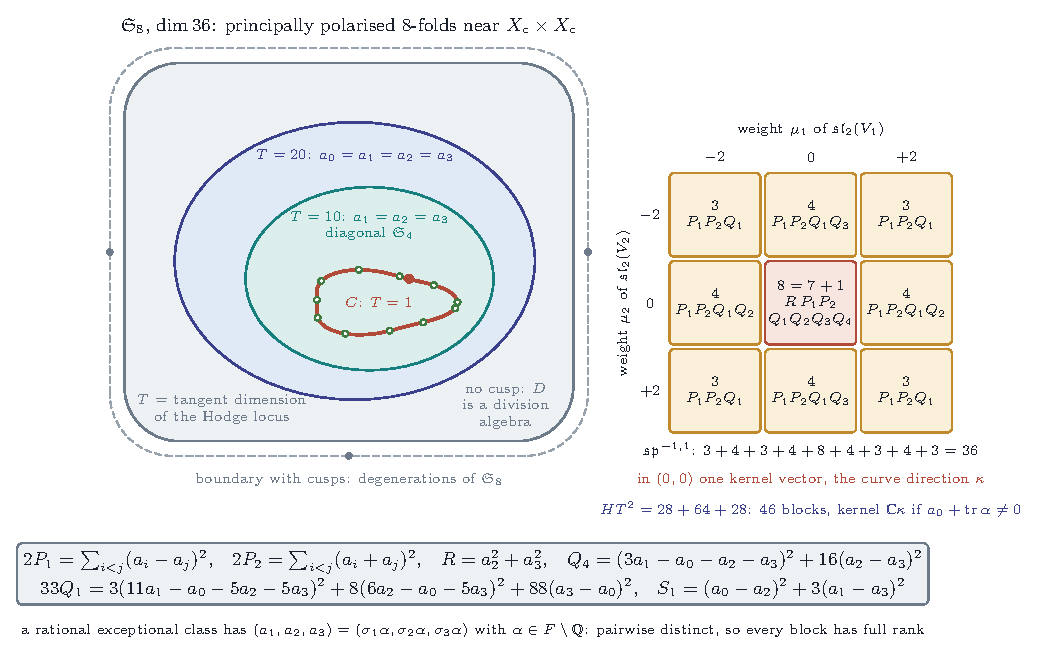
\includegraphics[width=\textwidth]{fig_rigidity}
\caption{\Cref{thm:mumfordrigid}. Left: the Siegel space $\mathfrak{S}$ of
dimension $36$ near $Y=X_{c}\times X_{c}$ and three Hodge loci through it,
labelled by the tangent dimension $T$ at $Y$: the class with equal
coefficients ($T=20$), the products of divisor classes with $a_{1}=a_{2}=a_{3}$
($T=10$, the diagonal Siegel space), and a rational exceptional class ($T=1$),
whose locus is the compact Mumford curve with its CM points (hollow). The
dashed rim is the boundary of $\mathfrak{S}$, which the curve does not reach.
Right: the nine weight blocks of $\mathfrak{sp}^{-1,1}$ under the torus of
the first two factors, with their dimensions and the forms whose product is
the Gram determinant of each; only the block of weight $(0,0)$ has a kernel,
the direction $\kappa$ of the curve. The same holds in the $46$ blocks of
$HT^{2}(Y)$ off the hyperplane $L_{0}=0$. Below: the sums of squares that
make the determinants nonzero at the conjugates of an irrational element of
$F$.}
\label{fig:rigidity}
\end{figure}

\begin{corollary}[No degeneration and no larger family]
\label{cor:nodegeneration}
Let $\omega$ be a rational exceptional class on $X_{c}\times X_{c}$. Every
connected complex analytic family of polarised abelian eightfolds through
$X_{c}\times X_{c}$ on which $\omega$ stays of Hodge type lies, near each
point of the curve, inside the curve $\{X_{t}\times X_{t}:t\in C\}$, which is
compact. In particular no such family degenerates, and on no member of it
other than the CM points of the curve is $\omega$ a combination of products
of divisor classes or of Weil classes of CM fields acting on the member or on
its quotients.
\end{corollary}

\begin{proof}
By \Cref{thm:mumfordrigid}(iii) the Hodge locus of $\omega$ coincides with the
curve in a neighbourhood of every point of the curve, so a connected family
through $Y$ on which $\omega$ stays of Hodge type maps into the curve near
each of its points over the curve; by connectedness and the identity theorem
its image is the curve. The curve is compact because $D$ is a division
algebra, so the arithmetic group of the Shimura curve is cocompact
\cite{Mum69}.\footnote{By \Cref{setup:mumford} the algebra $D$ is definite at
$\sigma_{1}$ and $\sigma_{2}$, so $D\otimes_{F,\sigma_{1}}\RR$ is Hamilton's
quaternions and $D$ is not $M_{2}(F)$: it is a division algebra, split at the
one real place $\sigma_{3}$. The norm one group of an order in it, embedded in
$\SL_{2}(\RR)$ through $\sigma_{3}$, is a Fuchsian group of finite covolume
with no parabolic element: a parabolic $\gamma\ne\pm1$ would make
$\gamma\mp1$ a nonzero nilpotent element of $D$. A Fuchsian group of finite
covolume without parabolic elements has compact quotient.} For the last sentence: a member of the curve other than a CM
point has Hodge group $G$ (proof of \Cref{cor:mumfordequiv}), and on it
$\omega$ lies outside the span of the products of divisor classes and of the
Weil classes of quotients, by \Cref{prop:mumfordproduct}(ii) and (iii). At a
CM point the class is algebraic already (\Cref{thm:mumfordcm}), and the
countably many CM points do not carry algebraicity to the other members
(\Cref{lem:spreading}).
\end{proof}

The same computation controls deformations that are not algebraic at all,
and so decides whether the twistor lines along which Markman moves sheaves
for Weil classes can be used here.

\begin{proposition}[The Hodge locus among all complex tori, and twistor
lines]\label{prop:notwistor}
Let $\omega$ be a rational exceptional class, $Y=X_{c}\times X_{c}$ with
$c\in C$, and $\Lambda=H_{1}(Y,\ZZ)$. Let $\mathcal{T}$ be the space of
complex structures on the real torus $\Lambda_{\RR}/\Lambda$, a complex
manifold of dimension $64$ with tangent space $H^{1}(T_{Y})$ at $Y$, and
$\mathcal{T}_{\omega}\subset\mathcal{T}$ the closed analytic subset on which
$\omega$ is of type $(2,2)$.
\begin{enumerate}[label=\textup{(\roman*)},leftmargin=2.6em,itemsep=2pt]
\item The connected component of $\mathcal{T}_{\omega}$ that contains $Y$ is
  the universal cover $\mathfrak{H}$ of the Mumford curve, the set of
  squares of members of the family, biholomorphic to the upper half plane.
  Every connected complex analytic family of complex tori, algebraic or not,
  through a member of the Mumford family on which $\omega$ stays of Hodge
  type lies in the family.
\item No twistor line through a member of the Mumford family, and no compact
  connected complex curve in $\mathcal{T}$ through it, keeps $\omega$ of
  Hodge type.
\item $\mathcal{T}_{\omega}$ contains twistor lines nevertheless. The algebra
  $D\otimes_{F,\sigma_{1}}\RR$ is Hamilton's quaternions and acts on
  $V_{\RR}$ through the first factor of $G(\RR)$; for a unit quaternion $j$
  with $j^{2}=-1$, the complex structure $j\oplus j$ on $V_{\RR}\oplus
  V_{\RR}$ makes $\omega$ of type $(2,2)$, and these structures form a twistor
  line. On each factor $\psi(x,jy)$ has signature $(4,4)$, and a member whose
  Mumford--Tate group is $G$ is not an abelian variety. These twistor lines
  lie in components of $\mathcal{T}_{\omega}$ other than $\mathfrak{H}$.
\end{enumerate}
\end{proposition}

\begin{proof}
(i) The complex structures on $\Lambda_{\RR}$ for which all the tensors
invariant under $G$ are of Hodge type are those $J$ with $J^{2}=-1$ in the
real points of $G\cdot\mathbb{G}_{m}$, since a reductive group containing the
homotheties is the stabiliser of its invariant tensors. Let $\mathfrak{H}$ be
the connected component of this closed set that contains $Y$; it is closed in
$\mathcal{T}$ and consists of the $J=1\otimes1\otimes j_{3}$ with
$j_{3}\in\SL_{2}(\RR)$, $j_{3}^{2}=-1$, in the half plane that contains the
structure of $Y$, that is of the squares of the members of the Mumford
family. At each of its points the
first order condition for $\omega$ to stay of type $(2,2)$ along
$\xi\in H^{1}(T_{Y})$ is $\xi\lrcorner\,\omega=0$, as in the proof of
\Cref{thm:mumfordrigid}(iii), where no polarisation was used, and by
\Cref{thm:mumfordrigid}(i) the solutions form the line $\CC\kappa$ tangent to
$\mathfrak{H}$. So near each of its points $\mathcal{T}_{\omega}$ is the smooth
curve germ of $\mathfrak{H}$, and $\mathfrak{H}$ is open in
$\mathcal{T}_{\omega}$. Being also closed and connected, it is a connected
component. A connected analytic family on which $\omega$ stays of Hodge type
maps into $\mathcal{T}_{\omega}$, hence into $\mathfrak{H}$ once one of its
points does.

(ii) A twistor line is a nonconstant holomorphic image of $\PP^{1}$ in
$\mathcal{T}$. If $\omega$ stayed of Hodge type along one through a point of
$\mathfrak{H}$, or along any compact connected curve through it, the curve
would lie in $\mathfrak{H}$ by (i), and a holomorphic map from a compact
connected curve to the upper half plane is constant.

(iii) At $\sigma_{1}$ the quaternion algebra $D$ is definite
(\Cref{setup:mumford}), so the first factor of $G(\RR)$ is the group of unit
quaternions, and $V_{\RR}$ restricted to it is a module over
$D\otimes_{F,\sigma_{1}}\RR\cong\mathbb{H}$. The unit quaternions $j$ with
$j^{2}=-1$ form a two-sphere, and the complex structures given by left
multiplication by them on a quaternionic vector space form a twistor line.
Each $j$ lies in $G(\RR)$, and so does the circle $\cos\vartheta+j\sin\vartheta$,
which fixes $\omega$; so $\omega$ is of type $(2,2)$. Item (XLVII) of
\Cref{sec:verification} realises $V_{\RR}$ inside $V_{1}\otimes V_{2}
\otimes V_{3}$ as the fixed space of the real structure that is quaternionic on
the first two factors and real on the third, and finds that $\psi(x,Jy)$ is
definite for the structures of the Mumford family and of signature $(4,4)$ for
$J=j\otimes1\otimes1$. At a member whose Mumford--Tate group is $G$, the Hodge
classes of degree two on $V_{\RR}\oplus V_{\RR}$ are the forms $\psi\otimes s$
with $s$ a symmetric $2\times2$ matrix, by \Cref{prop:mumfordproduct}(ii), and
the signature of $\psi(\cdot,J\cdot)\otimes s$ is $(4(p+q),4(p+q))$ when $s$ has
signature $(p,q)$, so none is definite, none is a polarisation, and the member
is not an abelian variety. The members of the Mumford family are not on these
lines, so by (i) the lines lie in other components.
\end{proof}

Markman's proof for Weil classes on abelian fourfolds moves a sheaf along
twistor lines on which its Chern character stays of Hodge type. By
\Cref{prop:notwistor} no such line passes through the square of a member of
the Mumford family: the twistor lines on which $\omega$ is of Hodge type exist,
but they carry non-algebraic tori whose Hodge cocharacter lies in a definite
factor of $D$, in components of the Hodge locus that the Mumford family never
meets. The Kuga--Satake class of \Cref{thm:mumfordks} behaves differently. The
Kuga--Satake construction applies to every Hodge structure of K3 type on
$(T,q_{\lambda})$, so that class stays of Hodge type over the whole period
domain of $(T,q_{\lambda})$, of dimension seven, and not only along the curve;
it is the one class attached to the target that deformation methods of this
kind are not excluded from.

The same space $T$ also makes the square a holomorphic symplectic variety,
and this decides what the mechanism of van Geemen and Rapagnetta would have
to supply here. They prove the Hodge conjecture for the general abelian
fourfold of Weil type with trivial discriminant by pulling back the second
Chern class of a hyperk\"ahler sixfold along a map from the fourfold, which
gives an algebraic class of codimension two that is not a product of divisor
classes \cite{vGR26}. For a projective hyperk\"ahler manifold $M$ write
$\sigma_{M}$ for its symplectic form, $q_{M}$ for its Beauville--Bogomolov
form and $T(M)$ for the orthogonal complement of $\NS(M)_{\QQ}$ in
$H^{2}(M,\QQ)$ for $q_{M}$.

\begin{proposition}[The square as a holomorphic symplectic
variety]\label{prop:hksquare}
Let $c\in C$ be a point at which the Mumford--Tate group of $X=X_{c}$ is
$G\cdot\mathbb{G}_{m}$, let $Y=X\times X$, and let $\Psi\in\bigwedge^{2}V$ be
the $G$-invariant bivector dual to $\psi$. For $x\in T$ put
$\iota(x)=(x\otimes1)\Psi$ in $V\otimes V=H^{1}(X,\QQ)\otimes H^{1}(X,\QQ)$, a
K\"unneth component of $H^{2}(Y,\QQ)$, and let $\iota_{2}\colon S^{2}T\to
H^{4}(Y,\QQ)$ be the map $xy\mapsto\iota(x)\cup\iota(y)$. Let $C_{i}\in
S^{2}T_{i}$ be the Casimir element of the trace form of
$\mathfrak{sl}(V_{i})$, and for $\nu\in F$ let
$c_{\nu}=\sum_{i}\sigma_{i}(\nu)C_{i}$, a rational element of $S^{2}T$; for
$\nu\ne0$ it is the element dual to the form $q_{1/\nu}$.
\begin{enumerate}[label=\textup{(\roman*)},leftmargin=2.6em,itemsep=2pt]
\item $\iota$ is an embedding of Hodge structures $T(-1)\to H^{2}(Y,\QQ)$, its
  image is the only irreducible sub-Hodge structure of $H^{2}(Y,\QQ)$ with
  $h^{2,0}=1$, and the holomorphic $2$-form $\sigma_{0}$ spanning its part of
  type $(2,0)$ is symplectic.
\item $\iota_{2}(c_{\nu})=\omega_{a}$ with $a_{0}=3\Tr_{F/\QQ}(\nu)$ and
  $\alpha=4\nu-\Tr_{F/\QQ}(\nu)$, in the notation of \Cref{setup:omegaa}. So
  $\iota_{2}(c_{\nu})$ is exceptional if and only if $\nu\notin\QQ$, and every
  rational exceptional class is some $\iota_{2}(c_{\nu})$ plus a rational
  multiple of $\pi_{0}$.
\item Let $M$ be a projective hyperk\"ahler manifold and
  $f\colon Y\dashrightarrow M$ a rational map with $f^{*}\sigma_{M}\ne0$. Then
  $f^{*}$ maps $T(M)$ isomorphically onto $\iota(T)$ and is compatible with
  products of classes in $T(M)$; $f$ is generically finite onto a subvariety
  of dimension eight on which $\sigma_{M}$ is generically nondegenerate;
  $b_{2}(M)\ge10$; and $\dim M\ge10$.
\item Suppose in (iii) that $M=S^{[n]}$ is the Hilbert scheme of $n$ points
  on a projective K3 surface $S$, and
  let $q_{\lambda}$ be the form on $T$ that corresponds to the intersection
  form of $S$ on $T(S)=T(M)$ under $\iota^{-1}f^{*}$
  (\Cref{prop:mumfordrm}(iii)). If $\lambda\notin\QQ$, or if the real
  multiplication of $T(S)$ is induced by algebraic cycles on $S\times S$,
  then the Hodge conjecture holds for $Y$.
\end{enumerate}
\end{proposition}

\begin{proof}
(i) The map $\iota$ is $G$-equivariant because $\Psi$ is invariant, and
injective. Its image lies in $S^{2}V$: for $x$ in the symplectic Lie algebra
of $\psi$ one has $(x\otimes1)\Psi=-(1\otimes x)\Psi$, and the exchange of the
two factors carries $(x\otimes1)\Psi$ to $-(1\otimes x)\Psi$ because $\Psi$
is alternating. An element $g$ of $G\cdot\mathbb{G}_{m}$ multiplies $\Psi$ by
the multiplier $\chi(g)$ of $\psi$, so $(g\otimes g)\iota(x)=
\chi(g)\,\iota(gxg^{-1})$: the map $\iota$ is equivariant for the adjoint
action on $T$ twisted by $\chi$, which is the action defining $T(-1)$. Both
Hodge structures come from the Hodge cocharacter through
$G\cdot\mathbb{G}_{m}$, so $\iota$ is a morphism of Hodge structures from
$T(-1)$. The sub-Hodge structures
of $H^{2}(Y,\QQ)$ are its $G$-stable subspaces, since $\mathbb{G}_{m}$ acts
by scalars. Over $\bar{\QQ}$, item (XLVIII) of \Cref{sec:verification} splits
$H^{2}(Y)=\bigwedge^{2}(V\oplus V)$ by the three Casimir operators into the
isotypic pieces of highest weights $(0,0,0)$, $(2,2,0)$, $(2,0,2)$,
$(0,2,2)$, $(2,2,2)$, $(2,0,0)$, $(0,2,0)$, $(0,0,2)$, of dimensions
$3,27,27,27,27,3,3,3$, whose parts of type $(2,0)$ have dimensions
$0,0,9,9,9,0,0,1$; the last three pieces are $\iota(T_{1})$, $\iota(T_{2})$,
$\iota(T_{3})$. So an irreducible summand of highest weight $(2,0,2)$ or
$(0,2,2)$ contributes $3$ to $h^{2,0}$, one of weight $(2,2,2)$ contributes
$9$, one of weight $(0,0,2)$ contributes $1$, and the others contribute
nothing. A rational sub-Hodge structure $W$ is stable under the Galois group,
which permutes the highest weights as it permutes the factors, transitively.
So if $W\otimes\bar{\QQ}$ has a summand of weight $(2,2,0)$, $(2,0,2)$ or
$(0,2,2)$, it has summands of all three and $h^{2,0}(W)\ge6$; if it has one of
weight $(2,2,2)$, then $h^{2,0}(W)\ge9$. If $h^{2,0}(W)=1$, therefore,
$W\otimes\bar{\QQ}$ contains the piece $\iota(T_{3})$ of weight $(0,0,2)$,
which has multiplicity one, and with it $\iota(T_{1})$ and $\iota(T_{2})$; so
$W\supseteq\iota(T)$, and $W=\iota(T)$ if $W$ is irreducible. The
part of type $(2,0)$ of $\iota(T)$ is spanned by $\sigma_{0}=\iota(E_{3})$,
where $E_{3}\in\mathfrak{sl}(V_{3})\otimes\CC$ maps $V_{3}^{0,1}$ onto
$V_{3}^{1,0}$, and item (XLVIII) finds that $\sigma_{0}$ pairs $H^{1,0}$ of the
first factor with $H^{1,0}$ of the second through an invertible matrix. So
$\sigma_{0}$ has rank eight: it is a holomorphic symplectic form on $Y$.

(ii) Item (XLVIII) computes
$\iota_{2}(C_{1})=3\pi_{0}-\pi_{12}-\pi_{13}+3\pi_{23}$ and the two cyclic
permutations of this identity, in the split model; both sides are built
from $\psi$ and the actions of the three factors, so the identities hold over
$\bar{\QQ}$ in \Cref{setup:mumford}. Summing with the coefficients
$\sigma_{i}(\nu)$ gives $\iota_{2}(c_{\nu})=3\Tr(\nu)\pi_{0}+
\sum\sigma_{k}(4\nu-\Tr(\nu))\pi_{ij}$, the sum over $\{i,j,k\}=\{1,2,3\}$ with
$i<j$, which is $\omega_{a}$ with the stated $a_{0}$ and $\alpha$. Since
$\Tr(\nu)\in\QQ$, the element $\alpha$ is rational exactly when $\nu$ is; and
$\Tr(\alpha)=\Tr(\nu)$, so $\nu=(\alpha+\Tr(\alpha))/4$ recovers $\nu$ from
any $\alpha\in F$. Two rational classes with the same $\alpha$ differ by a
multiple of $\pi_{0}$. The Casimir element $C_{i}$ is dual to the trace form
on $T_{i}$, so $c_{\nu}$ is dual to $\sum_{i}\sigma_{i}(\nu)^{-1}
\operatorname{tr}(x_{i}y_{i})=q_{1/\nu}(x,y)$.

(iii) Resolve the indeterminacy of $f$ by a sequence of blow-ups along
smooth centres, $\pi\colon\tilde{Y}\to Y$ and $\tilde{f}\colon\tilde{Y}\to M$,
and put $f^{*}=\pi_{*}\tilde{f}^{*}$, a morphism of Hodge structures. The
kernel of $\pi_{*}$ on $H^{2}(\tilde{Y},\QQ)$ is spanned by the classes of
the exceptional divisors, so $\alpha\mapsto\tilde{f}^{*}\alpha-
\pi^{*}f^{*}\alpha$ is a morphism of Hodge structures from $H^{2}(M,\QQ)$ to a
space of Hodge classes. The Hodge structure $T(M)$ is irreducible. A
sub-Hodge structure $W\subseteq T(M)$ with $W^{2,0}=0$ consists of rational
classes of type $(1,1)$, which lie in $\NS(M)_{\QQ}\cap T(M)=0$; if
$W^{2,0}\ne0$, then $\sigma_{M}\in W_{\CC}$, the orthogonal complement of $W$
in $H^{2}(M,\QQ)$ is a sub-Hodge structure orthogonal to $\sigma_{M}$ and
$\bar{\sigma}_{M}$, hence of type $(1,1)$ and contained in $\NS(M)_{\QQ}$,
and $W\supseteq T(M)$. It is not spanned by Hodge classes, so that
morphism vanishes on it, and $\tilde{f}^{*}\alpha=\pi^{*}f^{*}\alpha$ for
$\alpha\in T(M)$. Since $\tilde{f}^{*}$ is a ring homomorphism and
$\pi_{*}\pi^{*}$ is the identity, $f^{*}(\alpha\beta)=f^{*}\alpha\cup
f^{*}\beta$ for $\alpha,\beta\in T(M)$. The kernel of $f^{*}$ on $T(M)$ is a
sub-Hodge structure not containing $\sigma_{M}$, hence zero, and the image is
irreducible with $h^{2,0}=1$, hence $\iota(T)$ by (i). So $f^{*}\sigma_{M}$ is
a nonzero multiple of $\sigma_{0}$ and has rank eight at every point of $Y$
where $f$ is defined; the rank of a pulled-back form is at most the dimension
of the image, so $f$ is generically finite onto its image $Z$, of dimension
eight, and $\sigma_{M}$ is generically nondegenerate on $Z$. As $M$ is
projective, $b_{2}(M)=\dim T(M)+\dim\NS(M)_{\QQ}\ge9+1$; this excludes the
generalised Kummer varieties, whose second Betti number is seven
\cite{Bea83}. Finally $\dim M\ge\dim Z=8$, and suppose $\dim M=8$. Then $f$
is dominant, and for $\alpha\in T(M)_{\CC}$ the relation of Fujiki and
Beauville \cite{Bea83,Fuj87} gives
\[
  \int_{Y}(f^{*}\alpha)^{8}=\int_{\tilde{Y}}\tilde{f}^{*}(\alpha^{8})
  =\deg(f)\int_{M}\alpha^{8}=\deg(f)\,c_{M}\,q_{M}(\alpha)^{4},
  \qquad c_{M}>0 .
\]
Write $f^{*}\alpha=\iota(x)$ with $x=x_{1}+x_{2}+x_{3}\in T_{\CC}$ and
$N_{i}=-\det x_{i}$. The form $x\mapsto q_{M}((f^{*})^{-1}\iota(x))$ is
invariant under $G$, so it is $q_{\lambda}(x,x)=
\sum_{i}\sigma_{i}(\lambda)\operatorname{tr}(x_{i}^{2})=
2\sum_{i}\sigma_{i}(\lambda)N_{i}$ for some $\lambda\in F^{\times}$ by
\Cref{prop:mumfordrm}(iii). On the other side, item (XLVIII) finds
$\iota(x)^{8}=8!\det(x)$ times a volume form, and
$\det(x_{1}\otimes1\otimes1+1\otimes x_{2}\otimes1+1\otimes1\otimes
x_{3})=\Delta(N_{1},N_{2},N_{3})^{2}$ with
$\Delta=N_{1}^{2}+N_{2}^{2}+N_{3}^{2}-2N_{1}N_{2}-2N_{1}N_{3}-2N_{2}N_{3}$;
this is also the product of the eight numbers $\pm r_{1}\pm r_{2}\pm r_{3}$,
where $\pm r_{i}$ are the eigenvalues of $x_{i}$ and $r_{i}^{2}=N_{i}$. The
$N_{i}$ are algebraically independent functions on $T_{\CC}$, so
$\Delta^{2}$ would be a constant multiple of the fourth power of the linear
form $\sum_{i}\sigma_{i}(\lambda)N_{i}$. But $\Delta$ is a nondegenerate
ternary quadratic form, hence irreducible, and a contradiction results. So
$\dim M\ge10$.

(iv) By \cite{Bea83} the map $H^{2}(S,\QQ)\to H^{2}(S^{[n]},\QQ)$ induced by
the universal subscheme $Z_{n}\subset S\times S^{[n]}$ is injective, carries
the intersection form to the Beauville--Bogomolov form, and has
$H^{2}(S^{[n]},\QQ)=H^{2}(S,\QQ)\oplus\QQ\delta$ with $\delta$ algebraic, so
$T(M)=T(S)$. Let $\Delta_{T}$ be the K\"unneth component in $T(S)\otimes
T(S)$ of the class of the diagonal of $S$; it is algebraic, being the class
of the diagonal minus $[\mathrm{pt}\times S]$, $[S\times\mathrm{pt}]$ and
$\sum_{r}d_{r}\times d_{r}^{\vee}$ over dual bases of $\NS(S)_{\QQ}$. Its image
under the correspondence $Z_{n}\times Z_{n}$, pulled back along the diagonal
of $M$, is the class $\sum_{a}e_{a}\cup e_{a}^{\vee}$ over dual bases of
$T(S)$ for the intersection form, which is therefore algebraic on $M$, and by
(iii) its image under $f^{*}$ is $\iota_{2}$ of the element of $S^{2}T$ dual
to $q_{\lambda}$, that is $\iota_{2}(c_{1/\lambda})$, an algebraic class on
$Y$. If $\lambda\notin\QQ$ it is exceptional by (ii). If instead the real
multiplication is algebraic, apply it to the first factor of $\Delta_{T}$:
for $b\in F$ the class $\sum_{a}(m_{b}e_{a})\cup e_{a}^{\vee}$ is algebraic,
and its image is $\iota_{2}(c_{b/\lambda})$, which is exceptional for
$b\notin\QQ\lambda$. In both cases \Cref{lem:oneexceptional} makes every
Hodge class in $H^{2}(X)\otimes H^{2}(X)$ algebraic; the Hodge classes in the
other K\"unneth components of $H^{4}(Y,\QQ)$ are products of divisor classes,
as at the end of the proof of \Cref{thm:mumfordks}; and the Hodge classes of
$Y$ form a ring generated in degrees two and four (proof of
\Cref{cor:mumfordequiv}).
\end{proof}

\begin{remark}[What the mechanism of van Geemen and Rapagnetta would
need]\label{rem:hkroute}
By \Cref{prop:hksquare}(ii) the exceptional classes are the classes
$\iota_{2}(c_{\nu})$ with $\nu\notin\QQ$, the images of the elements dual to
the forms $q_{\lambda}$, $\lambda=1/\nu$, on the part $\iota(T)$ of $H^{2}(Y)$
generated by the symplectic class; the form with $\lambda$ rational gives a
product of divisor classes. They are the analogues
for $(Y,\sigma_{0})$ of the dual Beauville--Bogomolov class, whose pull-back is
what \cite{vGR26} uses. Part (iii) says what a transfer of that argument
needs: a projective hyperk\"ahler manifold of dimension at least ten with
transcendental part $T(-1)$, such as $S_{\mu}^{[n]}$ with $n\ge5$ for a
surface $S_{\mu}$ of \Cref{thm:mumfordks}, and a rational map from $Y$ onto a
symplectic subvariety of dimension eight. For $M=S_{\mu}^{[n]}$ the form of
(iv) is $q_{\mu/e^{2}}$ for the $e\in F^{\times}$ with $\iota^{-1}f^{*}=m_{e}$
on $T(S_{\mu})=T$, so $\lambda\notin\QQ$ for every such map as soon as
$\mu\notin\QQ^{\times}F^{\times2}$. No such map is known. It would give an
algebraic cycle on $S_{\mu}\times X\times X$ inducing an isomorphism of
$T(S_{\mu})$ onto $\iota(T)\subset H^{1}(X)\otimes H^{1}(X)$, a correspondence
of the kind that the Kuga--Satake class supplies in the proof of
\Cref{thm:mumfordks}; so this is the Kuga--Satake route in geometric form,
not an independent one. Maps to K3 surfaces and to hyperk\"ahler eightfolds
cannot serve, by (iii).
\end{remark}

\begin{theorem}[The Mumford criterion is a dimension]
\label{thm:mumfordnumerical}
Let $c\in C$, $Y=X_{c}\times X_{c}$, $\omega=\omega_{a}$ a rational
exceptional class with $L_{0}(a)\ne0$, and $E$ a perfect complex on $Y$ with
$\ch(E)=N\omega$, $N\ne0$, and no other component.
\begin{enumerate}[label=\textup{(\roman*)},leftmargin=2.6em,itemsep=2pt]
\item $\dim\Ext^{2}(E,E)\ge119$.
\item If $\dim\Ext^{2}(E,E)=119$, then $\operatorname{ev}_{E}\colon
  HT^{2}(Y)\to\Ext^{2}(E,E)$ is surjective with kernel $\CC\kappa$, and
  $\sigma_{E}$ is injective. Conversely, if $\sigma_{E}$ is injective, then
  $\operatorname{ev}_{E}$ has rank $119$ and kernel $\CC\kappa$, and $E$
  extends to first order along the curve.
\item If some such $E$ at one point $c$ has $\dim\Ext^{2}(E,E)=119$, then
  $\omega_{t}$ is algebraic for every $t\in C$, the Hodge conjecture holds for
  $X_{t}\times X_{t}$ for every $t$, and $B(W\times_{C}W)$ holds.
\item At every CM point $c$ some perfect complex $E$ on $Y$ has
  $\ch(E)=N\omega$ for some $N\ne0$ and no other component.
\end{enumerate}
\end{theorem}

\begin{proof}
(i) and (ii). By the square $\sigma_{E}\circ\operatorname{ev}_{E}=
(\,\cdot\,)\lrcorner\,\ch(E)$ of \Cref{setup:criterion}, $\ker
\operatorname{ev}_{E}\subseteq\Ann_{HT^{2}}(\omega)=\CC\kappa$ by
\Cref{thm:mumfordrigid}(ii), so $\operatorname{ev}_{E}$ has rank at least
$119$, which is (i). If $\dim\Ext^{2}(E,E)=119$, then
$\operatorname{ev}_{E}$ is onto, its kernel has dimension one and lies in
$\CC\kappa$, so equals it; and $\sigma_{E}(\operatorname{ev}_{E}(x))=
N\,x\lrcorner\,\omega$ vanishes only for $x\in\CC\kappa=\ker
\operatorname{ev}_{E}$, so $\sigma_{E}$ is injective on
$\image\operatorname{ev}_{E}=\Ext^{2}(E,E)$. Conversely, if $\sigma_{E}$ is
injective, then $\sigma_{E}(\operatorname{ev}_{E}(\kappa))=N\kappa\lrcorner
\,\omega=0$ forces $\operatorname{ev}_{E}(\kappa)=0$, so the kernel is
$\CC\kappa$ and the rank is $119$; and $\operatorname{ev}_{E}$ restricted to
$H^{1}(T_{Y})$ is the obstruction map \cite{Tod09}, which vanishes at
$\kappa$.

(iii) By (ii) $\sigma_{E}$ is injective. The Chern character of $E$ is
$N\omega$, a flat section of Hodge type over the whole of $C$, so
\Cref{thm:BF} applies to every infinitesimal deformation of $Y$ inside
$W\times_{C}W\to C$. The proof of \Cref{thm:semiregclosure} now applies word
for word, with the stack of perfect complexes on the fibres of $W\times_{C}
W\to C$ \cite{Lie06} in place of that of $\cA\to\cS$, or the analytic
Kuranishi germ if $\Ext^{<0}(E,E)\ne0$: it is smooth over $C$ at $[E]$, its
image contains a nonempty open subset $U\subseteq C$, and for $t\in U$ a
perfect complex $E_{t}$ on $X_{t}\times
X_{t}$ in the same connected component has $\ch(E_{t})=N\omega_{t}$, so
$\omega_{t}$ is algebraic, and by \Cref{lem:oneexceptional} so are both
exceptional classes. $U$ is uncountable, and \Cref{cor:mumfordequiv} gives
the rest.

(iv) By \Cref{thm:mumfordcm} there is $\xi\in\CH^{2}(Y)_{\QQ}$ with class
$\omega$, and the argument of \Cref{prop:ktheory} gives $E$: the Chern
character is an isomorphism $K_{0}(Y)_{\QQ}\to\CH^{*}(Y)_{\QQ}$
\cite[Ex.~15.2.16(b) and Cor.~18.3.2]{Ful98}, so $\xi=\ch(u)$ for a unique
$u$, and $Nu$ is the class of a perfect complex for a suitable $N$.
\end{proof}

Part (iii) is the Mumford analogue of \Cref{thm:p2numerical}(iii): one object,
at one point, and one number, which is $119$ here and $2n(2n-1)$ for a Weil
family. For a Weil family that number is attained by no object
(\Cref{thm:p2false}), because an object attaining it would have to deform to
non-algebraic tori; the classes here are rigid, so that argument does not
apply (\Cref{rem:p2prime}). The objects of (iv) exist, and the only open question is whether one
of them, or another representative of the same class in $K_{0}$, attains the
bound of (i). We have not found one, and we do not claim that one exists. The
rigidity of \Cref{thm:mumfordrigid} is not an obstacle to it: semiregularity
moves an object along the Hodge locus of its Chern character, and the curve
is exactly that locus, so a semiregular object would propagate along the
curve and nowhere else, which is all that is needed.

\begin{corollary}[Bounded data at CM points]\label{cor:mumfordbounded}
Fix a relatively ample line bundle on $W\times_{C}W\to C$, and let $\omega$ be
a rational exceptional class. The following are equivalent.
\begin{enumerate}[label=\textup{(\alph*)},leftmargin=2.6em,itemsep=2pt]
\item $\omega_{t}$ is algebraic for every $t\in C$; equivalently, by
  \Cref{lem:oneexceptional} and \Cref{cor:mumfordequiv}, the Hodge conjecture
  holds for $X_{t}\times X_{t}$ for every $t\in C$.
\item There are a finite set $\Phi$ of pairs $(\underline{P},\underline{q})$,
  each a tuple of Hilbert polynomials with a tuple of rational numbers of the
  same length, and infinitely many points $c\in C$ at each of which
  $\omega_{c}=\sum_{i}q_{i}[Z_{i}]$ for subschemes $Z_{i}\subset X_{c}\times
  X_{c}$ with Hilbert polynomials $P_{i}$, for some $(\underline{P},
  \underline{q})\in\Phi$.
\end{enumerate}
In particular the classes are algebraic on every member as soon as they are
represented at infinitely many CM points by cycles of bounded degree.
\end{corollary}

\begin{proof}
For a pair $(\underline{P},\underline{q})$ let $\Sigma_{\underline{P},
\underline{q}}\subseteq C$ be the set of points at which $\omega$ is
represented with these data. The proof of \Cref{thm:closedlocus} applies
verbatim to $(W\times_{C}W,C,\omega)$, as in \Cref{lem:spreading}, and shows
that each $\Sigma_{\underline{P},\underline{q}}$ is Zariski closed. If (b)
holds, one pair of $\Phi$ serves at infinitely many points, so its
$\Sigma$ is an infinite closed subset of the irreducible curve $C$, hence
$C$, and (a) holds. If (a) holds, $C$ is the union of the countably many
$\Sigma_{\underline{P},\underline{q}}$, and $C$ is uncountable, so one of
them is infinite, hence equal to $C$; then (b) holds with $\Phi$ that one
pair and every point of $C$.
\end{proof}

\Cref{thm:mumfordcm} gives a representation at every CM point, through
Markman's theorem for abelian fourfolds \cite{Mar25a} and the ring of
\Cref{thm:mumfordcm}, with no control of degree, and isogenies between CM
members, which move CM points along their Hecke orbits, do not bound it
either. \Cref{cor:mumfordbounded} says that such a bound is not a convenience
but the whole remaining content: with it the target falls, and without it the
CM points, being countable, say nothing about a very general member
(\Cref{lem:spreading} needs uncountably many points).

\begin{remark}[The bypass mechanisms, one by one]\label{rem:bypassaudit}
\Cref{fig:bypass} collects what is known about each route to the Mumford
target that avoids the Lefschetz standard conjecture.
\begin{enumerate}[label=\textup{(\arabic*)},leftmargin=2.6em,itemsep=2pt]
\item \emph{Degeneration.} Blocked: the base is compact and the Hodge locus is
  the base (\Cref{cor:nodegeneration}), so no family on which $\omega$ stays
  of Hodge type approaches the boundary, and there is no limit mixed Hodge
  structure to specialise to.
\item \emph{Deformation into a larger Hodge locus}, on which $\omega$ would
  become a product of divisor classes or a Weil class and be algebraic by
  an earlier theorem, then be carried back. Blocked by
  \Cref{thm:mumfordrigid}(iii), already to first order.
\item \emph{Hochschild deformations}: twisting $D^{b}(Y)$ by a $B$-field or a
  Poisson bivector, as in the gerby and noncommutative deformations used for
  Weil classes. Blocked: an object with $\ch(E)=N\omega$ extends along no
  direction of $HH^{2}(Y)$ except that of the curve
  (\Cref{cor:mumfordsplit}(i)).
\item \emph{Constructions from line bundles}: cones, tensor products, duals,
  pull-backs and push-forwards along homomorphisms, and Fourier--Mukai
  functors whose kernels are built in the same way. Blocked at every point of
  the curve: everything so built has a Chern character invariant under the
  Lefschetz group, and the exceptional classes are not
  (\Cref{thm:lefschetzclosure}).
\item \emph{Twistor and hyperholomorphic deformation}, the mechanism of
  Markman's proof for Weil classes: move a sheaf along twistor lines on which
  its Chern character stays of Hodge type. Blocked on the square: no twistor
  line through a member of the Mumford family keeps $\omega$ of Hodge type,
  and those that do carry non-algebraic tori, in other components of the
  Hodge locus (\Cref{prop:notwistor}).
\item \emph{Specialisation.} The class is algebraic at every CM point
  (\Cref{thm:mumfordcm}), on every power of $X_{c}$ \cite[Theorem~1.3]{Li26};
  this suffices exactly when the degrees are bounded
  (\Cref{cor:mumfordbounded}), and no bound is known.
\item \emph{Reduction modulo $p$.} At every closed point of every reduction
  of the curve the class is a $\QQ_{\ell}$-combination of algebraic cycles
  (\Cref{prop:modp}), by Li's theorem \cite[Theorem~1.1]{Li26}; this
  suffices, with no lifting step, exactly when the Hilbert data of the cycles
  are bounded on a Zariski dense set of closed points of the arithmetic model
  (\Cref{thm:modpdensity}), and no bound is known.
\item \emph{Semiregularity.} Reduced to one dimension count at one CM point
  (\Cref{thm:mumfordnumerical}); an object attaining it has large odd
  self-extensions (\Cref{thm:mumfordprofile}), is not built from line
  bundles (\Cref{prop:mumforddivisor}) and splits only in a constrained way
  (\Cref{cor:mumfordsplit}); no such object is known.
\item \emph{Kuga--Satake.} Reduced to the Kuga--Satake class of one K3 surface
  of Picard number thirteen (\Cref{thm:mumfordks}), which the known cases do
  not reach (\Cref{rem:mumfordks}). Its geometric form is the mechanism of
  van Geemen and Rapagnetta \cite{vGR26}, pull-back of the dual
  Beauville--Bogomolov class of a hyperk\"ahler manifold: the exceptional
  classes are exactly such twisted dual forms of the part of $H^{2}$ of the
  square generated by its symplectic class, and a rational map onto a
  symplectic subvariety of some $S_{\mu}^{[n]}$, $n\ge5$, would suffice;
  K3 surfaces and hyperk\"ahler eightfolds cannot serve
  (\Cref{prop:hksquare}, \Cref{rem:hkroute}).
\item \emph{Motivated classes.} Every Hodge class on an abelian variety is
  motivated \cite[Th\'eor\`eme~0.6.2]{And96b}, so $\omega_{t}$ is motivated for
  every $t$; a motivated class is algebraic once the Lefschetz involutions of
  the auxiliary varieties are (\Cref{prop:lefmot}), and for the auxiliary
  varieties of Andr\'e's proof that is not known. Along the family the auxiliary variety
  that suffices is $W\times_{C}W$ (\Cref{thm:lefschetzpropagation}), and its
  Lefschetz standard conjecture is equivalent to the target
  (\Cref{cor:mumfordequiv}): the route moves the problem and does not shorten
  it.
\end{enumerate}
Five of the ten are closed off by theorems; two work at special points
only, the CM points and the closed points of the reductions modulo $p$, and
each of them suffices exactly when a degree bound holds; two are reduced to a
single object, one Kuga--Satake class or one perfect complex with
$\dim\Ext^{2}=119$ at one CM point; and one is equivalent to the target. None
of them is carried out here, and the target remains open. The five that are
not closed off are one statement and two stronger inputs, not five
obligations: any one of them would suffice (\Cref{cor:mumfordone},
\Cref{rem:mumfordneeded}).
\end{remark}

\begin{figure}[tbp]
\centering
  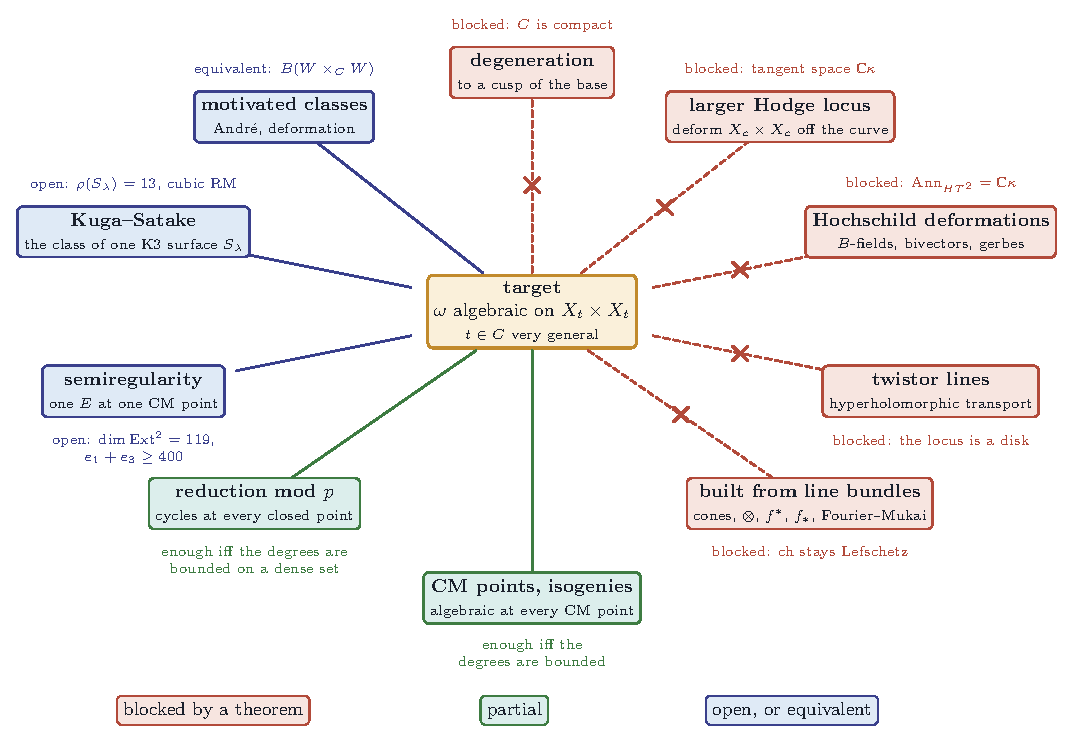
\includegraphics[width=0.96\textwidth]{fig_bypass}
\caption{\Cref{rem:bypassaudit}: the ten routes to the Mumford target that
avoid the Lefschetz standard conjecture. Clay, with a crossed dashed spoke: a
route closed off by a theorem of \Cref{ssec:mumfordrigid} or
\Cref{ssec:mumfordobject}. Grass: a route that works at special points only,
at the CM points or at the closed points of the reductions modulo $p$, and
suffices exactly when a degree bound holds (\Cref{cor:mumfordbounded},
\Cref{thm:modpdensity}). Indigo: a route reduced to one open statement, of
the same kind as the target or equivalent to it.}
\label{fig:bypass}
\end{figure}

\subsection{What an object meeting the Mumford criterion must look like, and
  the target modulo $p$}
\label{ssec:mumfordobject}

\Cref{thm:mumfordnumerical} reduces the semiregularity route to one object at
one CM point. This subsection derives what any object with the right Chern
character must satisfy, whether or not it is semiregular: no sequence of
standard operations produces it from line bundles, it extends along no first
order deformation of $D^{b}(Y)$ other than the direction of the curve, a
semiregular one splits only into summands with no $\Ext^{2}$ between them,
and its self-extensions are large in every degree, with an odd part that the
Euler characteristic forces beyond what Hochschild cohomology supplies. It
then turns to the reduction modulo $p$, after the recent proof of the Tate
conjecture for powers of abelian fourfolds over finite fields: the classes
are represented by cycles at every closed point of every reduction of the
curve, and the target is equivalent to a bound on those cycles on a Zariski
dense set of closed points. None of this constructs the object or closes the
target.

\begin{lemma}[The contraction ranks are symmetric]\label{lem:rankduality}
Let $A$ be an abelian variety of dimension $g$ and $c\in H^{*}(A,\CC)$ a class
each of whose components has Hodge type $(p,p)$ for some $p$. For $k\ge0$ put
$r_{k}(c)=\dim\bigl(HT^{k}(A)\lrcorner\,c\bigr)$, with the action of
\Cref{setup:hh}. Then $r_{k}(c)=r_{g-k}(c)$ for $0\le k\le g$, and
$r_{k}(c)=0$ for $k>g$.
\end{lemma}

\begin{proof}
Write $H^{1,0}=H^{1,0}(A)$ and $A'=H^{0,1}(A)$, both of dimension $g$, so
that $H^{*}(A,\CC)=\bigwedge^{*}H^{1,0}\otimes\bigwedge^{*}A'$ and
$HT^{*}(A)=\bigwedge^{*}(A'\oplus T)$ with $T=(H^{1,0})^{\vee}$. Fix a
generator of $\bigwedge^{g}A'$ and let
$\star\colon\bigwedge^{q}A'\to\bigwedge^{g-q}A'^{\vee}$ send $\eta$ to
$\zeta\mapsto\eta\wedge\zeta$. Under $\Phi=\mathrm{id}\otimes\star$, wedging
with $z\in A'$ becomes, up to a sign fixed on each bigraded piece, contraction
with $z$ on the second factor, while $T$ still contracts the first. So $\Phi$
identifies the action of $HT^{*}(A)$ with the action of
$\bigwedge^{*}U^{\vee}$ by interior products on $\bigwedge^{*}U$, where
$U=H^{1,0}\oplus A'^{\vee}$ has dimension $2g$, up to signs that do not change
ranks. A class of type $(p,p)$ goes to
$\bigwedge^{p}H^{1,0}\otimes\bigwedge^{g-p}A'^{\vee}\subset\bigwedge^{g}U$,
so $\eta=\Phi(c)$ lies in the middle degree whatever the $p$ of its
components. Hence $r_{k}(c)$ is the rank of
$\bigwedge^{k}U^{\vee}\to\bigwedge^{g-k}U$, $x\mapsto\iota_{x}\eta$, which is
zero for $k>g$. Its transpose for the natural pairings is
$\bigwedge^{g-k}U^{\vee}\to\bigwedge^{k}U$, $y\mapsto\pm\iota_{y}\eta$,
because $\langle\iota_{x}\eta,y\rangle=\langle\eta,x\wedge y\rangle
=\pm\langle\iota_{y}\eta,x\rangle$. A map and its transpose have the same
rank.
\end{proof}

\begin{theorem}[The self-extensions of an object with an exceptional Chern
character]\label{thm:mumfordprofile}
Let $c\in C$ and $Y=X_{c}\times X_{c}$, and write
$e_{k}=\dim\Ext^{k}(E,E)$ for a perfect complex $E$ on $Y$.
\begin{enumerate}[label=\textup{(\roman*)},leftmargin=2.6em,itemsep=2pt]
\item For every $E$ and every $k$, $e_{k}\ge r_{k}(\ch E)$ and
  $e_{k}=e_{8-k}$.
\item For a rational exceptional class $\omega=\omega_{a}$ with
  $L_{0}(a)\ne0$: $r_{0}=r_{8}=1$, $r_{1}=r_{7}=16$ and $r_{2}=r_{6}=119$.
\item There is a set of rational exceptional classes, Zariski dense in the
  space of rational Hodge classes in $H^{2}\otimes H^{2}$, on which
  \[
    \bigl(r_{0},\dots,r_{8}\bigr)(\omega)\;\ge\;
    (1,16,119,328,560,328,119,16,1)
  \]
  term by term. When $F$ is the cubic subfield of $\QQ(\zeta_{7})$ it contains
  the class with $a_{0}=2$ and $(a_{1},a_{2},a_{3})$ the conjugates of
  $\zeta_{7}+\zeta_{7}^{-1}$.
\item Let $\omega$ be in the set of (iii) and $\ch(E)=N\omega$ with $N\ne0$.
  Then
  \[
    e_{1}+e_{3}=e_{0}+e_{2}+\tfrac12e_{4}
      +\sum_{j\ge1}(-1)^{j}e_{-j}.
  \]
  If $\Ext^{<0}(E,E)=0$, for instance if $E$ is a sheaf, then
  $\sum_{k\ \mathrm{odd}}e_{k}=\sum_{k\ \mathrm{even}}e_{k}\ge800$,
  $e_{1}+e_{3}\ge400$, and $\sum_{k}e_{k}\ge1600$, while the bounds of
  (iii) add up to $1488$: the odd degrees carry at least $112$ dimensions
  beyond the Hochschild bound $2(16+328)=688$.
\end{enumerate}
\end{theorem}

\begin{proof}
(i) The square $\sigma_{E}\circ\operatorname{ev}_{E}=(\,\cdot\,)\lrcorner
\ch(E)$ of \Cref{setup:hh} holds in every degree, so the kernel of
$\operatorname{ev}_{E}$ on $HT^{k}(Y)$ lies in the annihilator of $\ch(E)$
and its image has dimension at least $r_{k}(\ch E)$. Serre duality with the
trivial canonical bundle gives $e_{k}=e_{8-k}$.

(ii) $r_{0}=1$ because $\omega\ne0$, and $r_{2}=119$ is
\Cref{thm:mumfordrigid}(ii). If $w\in HT^{1}(Y)$ annihilates $\omega$, so does
$w'\wedge w$ for every $w'\in HT^{1}(Y)$, since the annihilator is a left
ideal; for $w\ne0$ these products span a space of dimension $15$, which cannot
lie in $\Ann_{HT^{2}}(\omega)=\CC\kappa$. So $r_{1}=16$, and
\Cref{lem:rankduality} gives $r_{8},r_{7},r_{6}$.

(iii) For each $k$ the set of $a\in\CC^{4}$ at which the contraction on
$HT^{k}(Y)$ into $\omega_{a}$ has rank at least the displayed number is Zariski
open, being the complement of the common zeros of minors, and item (XLV) of
\Cref{sec:verification} shows that it contains $a=(3,5,-7,11)$, by an exact
computation over $\QQ$ block by block. The rational Hodge classes in
$H^{2}\otimes H^{2}$ form a $\QQ$-vector space of dimension four whose complex
span is $\CC^{4}$ (\Cref{setup:omegaa}), hence Zariski dense, and so they
meet the intersection of these open sets in a Zariski dense set; the classes
with $\alpha\in\QQ$ form a proper linear subspace and are removed. Item (XLV)
also computes the ranks modulo a prime at which the minimal polynomial of
$\zeta_{7}+\zeta_{7}^{-1}$ splits, for $a_{0}=2$ and the three conjugates in
each of the six orders, and finds the displayed numbers; a rank modulo a prime
of good reduction is a lower bound for the rank in characteristic zero.

(iv) Since $\ch(E)$ has only a component in $H^{4}$, $\ch(E^{\vee})\ch(E)$
lies in $H^{8}(Y)$ and $\chi(E,E)=\int_{Y}\ch(E^{\vee})\ch(E)=0$, the Todd
class being trivial. By (i) and Serre duality, which also pairs
$\Ext^{-j}$ with $\Ext^{8+j}$,
\[
  0=\chi(E,E)=2(e_{0}-e_{1}+e_{2}-e_{3})+e_{4}
  +2\sum_{j\ge1}(-1)^{j}e_{-j},
\]
which is the identity. With no negative extensions the odd and even parts are
equal, and the even part is at least $2\cdot1+2\cdot119+560=800$ by (i) and
(iii), so the odd part is at least $800$ as well, and $e_{1}+e_{3}\ge400$ by
Serre duality. The Hochschild bound on the odd part is $2(16+328)=688$.
\end{proof}

\begin{figure}[tbp]
\centering
  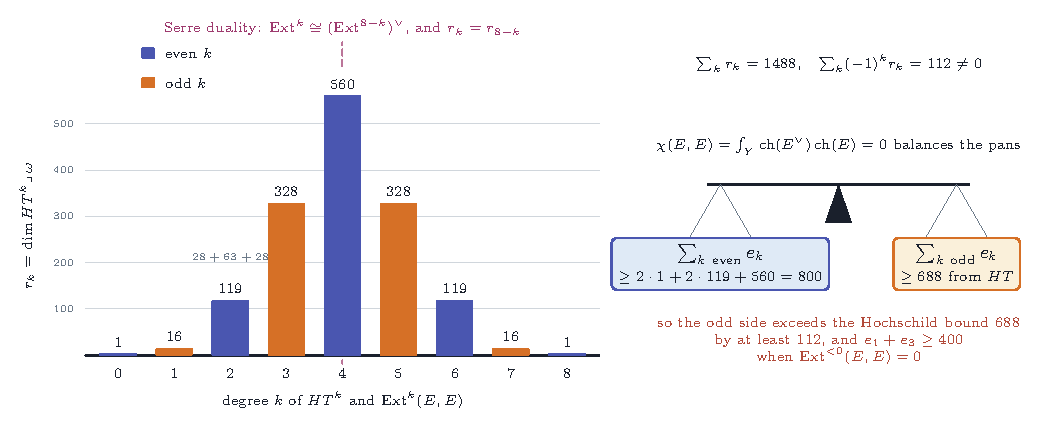
\includegraphics[width=\textwidth]{fig_extprofile}
\caption{\Cref{thm:mumfordprofile}. Left: the lower bounds $r_{k}$ for
$\dim\Ext^{k}(E,E)$ when $\ch(E)=N\omega$, one bar per degree, symmetric about
$k=4$ as \Cref{lem:rankduality} predicts; the bar at $k=2$ is the $119$ of
\Cref{thm:mumfordrigid}, made of $28$ classes in $H^{0,2}$, $63$ in
$H^{1}(T)$ and $28$ bivectors. On the hyperplane $L_{0}=0$ the bars at $2$,
$4$ and $6$ drop to $110$, $548$ and $110$ at a sample point. Right: $\chi(E,E)=0$ balances the
even and the odd degrees, so the odd side, which Hochschild cohomology fills
only to $688$, carries at least $800$.}
\label{fig:extprofile}
\end{figure}

\begin{proposition}[Divisor classes do not reach the exceptional classes]
\label{prop:mumforddivisor}
Let $t\in C$ and let $\omega$ be a rational exceptional class. Then $\omega_{t}$
is not in the $\QQ$-span of products of divisor classes of $X_{t}\times
X_{t}$: that span meets the rational Hodge classes of $H^{2}\otimes H^{2}$
exactly in the classes with $\alpha\in\QQ$. Consequently no perfect complex
whose Chern character lies in the subring generated by divisor classes, in
particular no bounded complex of direct sums of line bundles, has
$\ch(E)=N\omega$ with $N\ne0$. At a CM point $c$ the fourfold $X_{c}$ has eight
Hodge classes in $H^{4}$, of which the products of divisor classes span six.
\end{proposition}

\begin{proof}
At a point with Hodge group $G$, the divisor classes of $X_{t}\times X_{t}$ are
the three classes of \Cref{prop:mumfordproduct}(ii), all invariant under
$\Sp(V,\psi)$, and so are their products; the $\Sp(V,\psi)$-invariant part of
$H^{2}\otimes H^{2}$ is spanned by $\pi_{0}$ and $\pi_{12}+\pi_{13}+\pi_{23}$,
the classes with $a_{1}=a_{2}=a_{3}$. At a CM point the Hodge group is a
maximal torus of $G$ (proof of \Cref{thm:mumfordcm}), so the Hodge classes
are the monomials of weight zero, and item (XLV) computes over $\QQ$: $16$
divisor classes, $132$ Hodge classes in degree four, products of divisor
classes spanning $100$ of them, and a span meeting that of the four $\pi$ in
exactly the classes with $a_{1}=a_{2}=a_{3}$. For a rational class these
coordinates are the conjugates of $\alpha$, which by \Cref{lem:conjugates} are
equal only if $\alpha\in\QQ$. The Chern character of a complex in the subring
generated by divisor classes has its component in $H^{4}$ in the span of
products of two divisor classes, which excludes $N\omega$. The last sentence
is the same computation for $X_{c}$.
\end{proof}

At a CM point the Hodge classes of $X_{c}$ in $H^{4}$ that are not products
of divisor classes are among the classes that \Cref{thm:mumfordcm} pulls back
along homomorphisms $X_{c}\times X_{c}\to X_{c}$; they are algebraic by
Markman's theorem \cite{Mar25a}. Li proves,
independently and more generally, that every Hodge class on every power of
every complex CM abelian fourfold is algebraic \cite[Theorem~1.3]{Li26},
which gives \Cref{thm:mumfordcm} for every power $X_{c}^{n}$ and not only the
square. \Cref{prop:mumforddivisor} says that an object with $\ch(E)=N\omega$
cannot have its Chern character in the subring generated by divisor classes,
so it cannot be assembled from line bundles alone. The next theorem shows that
no sequence of the standard operations of the derived category, applied to
line bundles on powers of $X_{t}$, gets any further.

\begin{theorem}[What line bundles generate]\label{thm:lefschetzclosure}
Let $t\in C$, $X=X_{t}$, and let $L(X)\subseteq\Sp(V,\psi)$ be the Lefschetz
group of $X$, the centraliser of $\End^{0}(X)$ in $\Sp(V,\psi)$. Let
$\mathcal{A}$ be the class of abelian varieties isogenous to a power of $X$;
through an isogeny $X^{n}\to B$ the group $L(X)$ acts diagonally on
$H^{*}(B,\QQ)$, and the action does not depend on the isogeny. Let
$\mathcal{L}$ be the smallest class of objects of the categories
$D^{b}(B)$, $B\in\mathcal{A}$, that contains the line bundles and is closed
under shifts, cones, derived tensor products, derived duals, translations,
the functors $Lf^{*}$ and $Rf_{*}$ for homomorphisms $f$ between members of
$\mathcal{A}$, and the Fourier--Mukai functors $\Phi_{K}\colon D^{b}(B)\to
D^{b}(B')$ with kernel $K\in\mathcal{L}$ on $B\times B'$.
\begin{enumerate}[label=\textup{(\roman*)},leftmargin=2.6em,itemsep=2pt]
\item Every object of $\mathcal{L}$ has an $L(X)$-invariant Chern character.
\item $L(X)=\Sp(V,\psi)$ if $t$ is not a CM point, and $L(X)$ is a maximal
  torus of $\Sp(V,\psi)$ if it is. In both cases the $L(X)$-invariant classes
  on $X\times X$ form the subring generated by divisor classes, of dimensions
  $1,3,6,10,15,10,6,3,1$, respectively $1,16,100,304,454,304,100,16,1$, in
  the degrees $0,2,\dots,16$.
\item No rational exceptional class $\omega_{t}$ is $L(X)$-invariant. Hence
  for no object $E\in\mathcal{L}$ on $X\times X$ and no $N\ne0$ is
  $\ch(E)-N\omega_{t}$ invariant under $L(X)$; in particular
  $\ch(E)\ne N\omega_{t}$.
\item The $\Sp(V,\psi)$-module generated by $\pi_{12}-\pi_{13}$ is
  irreducible, of highest weight $2\varpi_{2}$ and dimension $308$, and it
  meets the span of the four $\pi$ in the plane of the classes with
  $a_{0}=0$ and $a_{1}+a_{2}+a_{3}=0$.
\end{enumerate}
\end{theorem}

\begin{proof}
(i) Two isogenies $X^{n}\to B$ differ by an element of $\End^{0}(X^{n})=
M_{n}(\End^{0}(X))$, which commutes with $L(X)$ acting diagonally, so the
action is well defined. For the same reason a homomorphism $f$ between members
of $\mathcal{A}$ is $L(X)$-equivariant on $H^{1}$, so $f^{*}$ is equivariant
on $H^{*}$, and so is $f_{*}$, which is $f^{*}$ conjugated by Poincar\'e
duality, since $L(X)\subseteq\SL(V)$ fixes the orientation classes.
Translations act trivially on cohomology. The Chern character is additive on
distinguished triangles and multiplicative on derived tensor products,
$\ch(E^{\vee})=\sum_{i}(-1)^{i}\ch_{i}(E)$, $\ch(Lf^{*}E)=f^{*}\ch(E)$, and
$\ch(Rf_{*}E)=f_{*}\ch(E)$ by the Grothendieck--Riemann--Roch theorem
\cite[Theorem~15.2]{Ful98}, the Todd class of an abelian variety being $1$;
and $\Phi_{K}=Rp_{2*}(p_{1}^{*}(\,\cdot\,)\otimes^{L}K)$. So the objects with
$L(X)$-invariant Chern character form a class with all the closure
properties, and it remains to see that it contains the line bundles, that is,
that $c_{1}(\mathcal{O}(D))$ is $L(X)$-invariant. Pulled back along an
isogeny, which is injective on rational cohomology, $c_{1}$ becomes a Hodge
class of degree two on some $X^{n}$, an element of the invariants of the
Hodge group in ${\textstyle\bigwedge^{2}}(V^{\vee}\otimes\QQ^{n})=
{\textstyle\bigwedge^{2}}V^{\vee}\otimes S^{2}\QQ^{n}\oplus S^{2}V^{\vee}
\otimes{\textstyle\bigwedge^{2}}\QQ^{n}$. If $t$ is not a CM point the Hodge
group is $G$, whose invariants in ${\textstyle\bigwedge^{2}}V$ are the multiples of $\psi$
and in $S^{2}V$ are zero, since every summand of $S^{2}(V_{1}\otimes V_{2}
\otimes V_{3})$ contains a factor $S^{2}V_{i}$; so the Hodge classes of degree
two are $\Sp(V,\psi)$-invariant. If $t$ is a CM point, a monomial of degree two
in a weight basis has weight zero for the Hodge torus exactly when its two
weights are opposite, and then it has weight zero for $L(X)$, by the
description in (ii).

(ii) If $t$ is not a CM point, $\End^{0}(X)=\QQ$ and $L(X)=\Sp(V,\psi)$. At a
CM point $\End^{0}(X)\otimes\CC$ is the algebra of diagonal matrices in a
weight basis (proof of \Cref{thm:mumfordcm}), and $\psi$ pairs each weight
with its opposite only, so $L(X)_{\CC}$ is the torus of diagonal matrices
$\operatorname{diag}(\lambda_{w})$ with $\lambda_{w}\lambda_{-w}=1$, of rank
four. For $t$ not CM, item (XLVI) of \Cref{sec:verification} bounds the
$\Sp(V,\psi)$-invariants of ${\textstyle\bigwedge^{*}}(V\oplus V)$ from above by the stated
dimensions and shows that products of the three divisor classes span spaces
of those dimensions. At a CM point the invariants are spanned by the
monomials of weight zero for $L(X)$; a set of weights $\pm e_{j}$ with sum
zero is a union of opposite pairs, so each such monomial is, up to sign, a
product of monomials of degree two and weight zero, which are divisor
classes, and item (XLVI) counts them: their numbers are the coefficients of
$(1+4y+y^{2})^{4}$.

(iii) If $t$ is not a CM point, the $\Sp(V,\psi)$-invariant combinations of the
$\pi$ are those with $a_{1}=a_{2}=a_{3}$ (\Cref{prop:mumforddivisor}), and
the coefficients of $\omega_{t}$ are the distinct conjugates of $\alpha$
(\Cref{lem:conjugates}). At a CM point use the map $x\mapsto E_{x}$ of the
proof of \Cref{lem:oneexceptional}, which is $\Sp(V,\psi)$-equivariant: it
carries $\omega_{t}$ to an element $(r,\beta)$ of $\QQ\times F$ with
$\beta\notin\QQ$, acting on $U_{ij}$ by the conjugate $\sigma_{k}(\beta)$
(\Cref{prop:mumfordrm}(ii)), and $\omega_{t}$ is $L(X)$-invariant only if
$E_{\omega_{t}}$ preserves the weight spaces of $L(X)$ in ${\textstyle\bigwedge^{2}}V$. Take
weight vectors $v=x\otimes y\otimes z$ and $w=x\otimes y'\otimes z'$ of
weights $(1,1,1)$ and $(1,-1,-1)$ for the Hodge torus. They are not
opposite, so $v\wedge w$ spans a weight space of $L(X)$, every weight of
$L(X)$ on $V$ having multiplicity one. But
$v\wedge w=(x\cdot x)\otimes\bigl(y\cdot y'\otimes z\wedge z'+y\wedge y'
\otimes z\cdot z'\bigr)$ has nonzero components in $U_{12}$ and in $U_{13}$,
on which $E_{\omega_{t}}$ acts by $\sigma_{3}(\beta)\ne\sigma_{2}(\beta)$. So
the line is not preserved. Item (XLVI) confirms the conclusion in exact
arithmetic: the components of $\pi_{12}$, $\pi_{13}$, $\pi_{23}$ of nonzero
weight for $L(X)$ span a space of dimension two, with the relation
$(1,1,1)$ only. The rest of (iii) follows from (i).

(iv) Item (XLVI) generates the module by applying the $36$ elements
$x\mapsto\psi(u,x)v+\psi(v,x)u$ of $\mathfrak{sp}(V,\psi)$ until the span
stops growing: it has dimension $308$ and highest weight $(2,2,0,0)$ for the
torus of diagonal matrices in $\Sp(V,\psi)$, and $308$ is, by Weyl's
dimension formula, the dimension of
the irreducible module of highest weight $2\varpi_{2}$; and adding the four
$\pi$ raises its dimension by two.
\end{proof}

\begin{remark}[Where a construction has to leave $\mathcal{L}$]
\label{rem:leavel}
\Cref{thm:lefschetzclosure} extends \Cref{prop:mumforddivisor} from sums of
line bundles to everything the standard operations make out of them, at every
point of the curve, including the CM points, where the exceptional classes
are algebraic: the cycles that represent them there are not Chern characters
of objects of $\mathcal{L}$, and neither are the two Hodge classes of $X_{c}$
in degree four that are not products of divisor classes. At a point that is
not CM every Chern character of an object of $\mathcal{L}$ lies in the
isotypic component of the trivial representation of $\Sp(V,\psi)$, while by
(iv) an object with $\ch(E)=N\omega$ must have a nonzero component in the one
of highest weight $2\varpi_{2}$. Every construction of such an object
therefore contains a step that does not commute with the Lefschetz group on
cohomology: passing to a direct summand, a subobject or a Jordan--H\"older
factor, choosing a point of a moduli space, or deforming from a member with
more endomorphisms. The last is what semiregularity does along the curve
(\Cref{thm:mumfordnumerical}).
\end{remark}

\begin{lemma}[The summands of a semiregular object]\label{lem:semiregsum}
Let $Z$ be a smooth projective variety and $E_{1},E_{2}$ perfect complexes on
$Z$. On $\Ext^{2}(E_{1}\oplus E_{2},E_{1}\oplus E_{2})=\bigoplus_{i,j}
\Ext^{2}(E_{j},E_{i})$ the semiregularity map is
$\sigma_{E_{1}\oplus E_{2}}(\zeta)=\sigma_{E_{1}}(\zeta_{11})
+\sigma_{E_{2}}(\zeta_{22})$. So $\sigma_{E_{1}\oplus E_{2}}$ is injective if
and only if $\sigma_{E_{1}}$ and $\sigma_{E_{2}}$ are, and
$\Ext^{2}(E_{1},E_{2})=\Ext^{2}(E_{2},E_{1})=0$.
\end{lemma}

\begin{proof}
The Atiyah class is natural, so $\mathrm{At}(E_{1}\oplus E_{2})$ is the
diagonal sum of $\mathrm{At}(E_{1})$ and $\mathrm{At}(E_{2})$. In
$\sigma(\zeta)=\sum_{q}\frac1{q!}\operatorname{tr}(\zeta\circ\mathrm{At}^{q})$
of \Cref{thm:BF} the composite $\zeta\circ\mathrm{At}^{q}$ has diagonal blocks
$\zeta_{ii}\circ\mathrm{At}(E_{i})^{q}$, and the trace of a block matrix of
morphisms is the sum of the traces of its diagonal blocks.
\end{proof}

\begin{corollary}[No Hochschild bypass, and no free splitting]
\label{cor:mumfordsplit}
Let $c\in C$, $Y=X_{c}\times X_{c}$, $\omega=\omega_{a}$ a rational
exceptional class with $L_{0}(a)\ne0$, and $E$ a perfect complex on $Y$ with
$\ch(E)=N\omega$, $N\ne0$.
\begin{enumerate}[label=\textup{(\roman*)},leftmargin=2.6em,itemsep=2pt]
\item $E$ extends to the first order deformation of $D^{b}(Y)$ given by
  $x\in HH^{2}(Y)=HT^{2}(Y)$ only if $x\in\CC\kappa$. No $B$-field, no
  Poisson bivector and no commutative deformation off the curve carries it.
\item If $\sigma_{E}$ is injective and $E=E_{1}\oplus E_{2}$ with both
  summands nonzero, then $\Ext^{2}(E_{1},E_{2})=\Ext^{2}(E_{2},E_{1})=0$, each
  $\sigma_{E_{i}}$ is injective, each $E_{i}$ extends to first order along the
  curve, and $\kappa\lrcorner\ch(E_{i})=0$. If moreover
  $\dim\Ext^{2}(E,E)=119$, then $\dim\Ext^{2}(E_{i},E_{i})=
  120-\dim\Ann_{HT^{2}}(\ch E_{i})$, and
  \[
    \Ann_{HT^{2}}(\ch E_{1})+\Ann_{HT^{2}}(\ch E_{2})=HT^{2}(Y),\qquad
    \Ann_{HT^{2}}(\ch E_{1})\cap\Ann_{HT^{2}}(\ch E_{2})=\CC\kappa .
  \]
\end{enumerate}
\end{corollary}

\begin{proof}
(i) The kernel of $\operatorname{ev}_{E}$ on $HH^{2}(Y)$ is the space of
deformations of $D^{b}(Y)$ along which $E$ deforms to first order
\cite{Tod09}, \cite[Section~8.3]{Mar25a}. If $\operatorname{ev}_{E}(x)=0$ then
$N\,x\lrcorner\,\omega=\sigma_{E}(\operatorname{ev}_{E}(x))=0$, so
$x\in\CC\kappa$ by \Cref{thm:mumfordrigid}(ii). The three kinds of
deformation named are the three summands of $HT^{2}(Y)$.

(ii) The first two assertions are \Cref{lem:semiregsum}. By
\Cref{thm:mumfordnumerical}(ii), $\operatorname{ev}_{E}(\kappa)=0$, and
$\operatorname{ev}_{E}$ is the diagonal sum of $\operatorname{ev}_{E_{1}}$
and $\operatorname{ev}_{E_{2}}$, so each vanishes at $\kappa$; then
$\kappa\lrcorner\ch(E_{i})=\sigma_{E_{i}}(\operatorname{ev}_{E_{i}}(\kappa))
=0$. Put $e(x)=120-\dim\Ann_{HT^{2}}(x)$, the rank of contraction into $x$.
It is subadditive, and by \Cref{thm:mumfordprofile}(i)
$\dim\Ext^{2}(E_{i},E_{i})\ge e(\ch E_{i})$. The cross terms vanish, so
\[
  119=\dim\Ext^{2}(E,E)=\sum_{i}\dim\Ext^{2}(E_{i},E_{i})
  \ge e(\ch E_{1})+e(\ch E_{2})\ge e(N\omega)=119,
\]
and every inequality is an equality. Hence
$\dim\Ann(\ch E_{1})+\dim\Ann(\ch E_{2})=121$. The intersection of the two
annihilators lies in $\Ann(N\omega)=\CC\kappa$ and contains $\kappa$, so it is
$\CC\kappa$, and the sum has dimension $120$.
\end{proof}

Part (ii) is the Mumford form of \Cref{thm:nosum}: a semiregular object
attaining the bound either does not split, or splits as two pieces whose
annihilators fill $HT^{2}(Y)$ and meet only in the direction of the curve, the
analogue of the two branches $P$ and $Q$ of \Cref{rem:twobranches}.

\begin{proposition}[Tate classes at every closed point of every reduction]
\label{prop:modp}
There are a finitely generated subring $R\subset\CC$, a model $W_{R}\to
C_{R}$ of $W\to C$ over $R$, with $C_{R}$ smooth and projective over $R$ with
geometrically connected fibres and $W_{R}$ an abelian scheme, projective over
$C_{R}$, and a finite surjective morphism $C'_{R}\to C_{R}$ from a second curve of the same
kind, with the following properties. Put $Y'=(W_{R}\times_{C_{R}}W_{R})
\times_{C_{R}}C'_{R}$, with projection $\pi'\colon Y'\to C'_{R}$, and let
$\omega$ be a rational exceptional class. For every prime $\ell$ there is a
global section $\omega_{\ell}$ of the lisse sheaf
$R^{4}\pi'_{*}\QQ_{\ell}(2)$ on $C'_{R}[1/\ell]$ whose restriction to
$C'_{R}\otimes_{R}\CC$ is the pull-back of $\omega\otimes1$; write
$\omega_{\ell}(\bar{x})$ for its value at a geometric point over a point $x$.
\begin{enumerate}[label=\textup{(\roman*)},leftmargin=2.6em,itemsep=2pt]
\item At a closed point $x$ of $C'_{R}[1/\ell]$ the residue field
  $\kappa(x)$ is finite, $Y'_{x}$ is the square of an abelian fourfold over
  it, and $\omega_{\ell}(\bar{x})$ is fixed by $\Gal(\bar{\kappa}/\kappa(x))$.
\item At such a point $\omega_{\ell}(\bar{x})$ is a $\QQ_{\ell}$-linear
  combination of classes of algebraic cycles of codimension two on $Y'_{x}$,
  defined over $\kappa(x)$.
\item Let $s$ be a closed point of $\Spec R[1/\ell]$ and $\eta_{s}$ the generic
  point of the reduction $C'_{s}$. Then $\omega_{\ell}(\bar\eta_{s})$ is fixed
  by the Galois group of the function field $\kappa(\eta_{s})$, and it is not
  a $\QQ_{\ell}$-linear combination of products of divisor classes of
  $Y'_{\bar\eta_{s}}$.
\end{enumerate}
Every closed point $x$ of a reduction $C_{s}$ of $C$ is the image of a closed
point $x'$ of $C'_{s}$, and $Y'_{x'}=Y_{x}\otimes_{\kappa(x)}\kappa(x')$; so
(i) and (ii) hold at every closed point of every reduction of $C$, after a
finite extension of its residue field.
\end{proposition}

\begin{proof}
\emph{The models.} The family $W\to C$ is defined over a subfield
$k_{1}\subset\CC$ finitely generated over $\QQ$, say as $W_{1}\to C_{1}$. Let
$K_{1}$ be the function field of $C_{1}$ and fix an embedding over $k_{1}$ of
an algebraic closure $\bar{K}_{1}$ into $\CC$; it sends the geometric generic
point of $C_{1}$ to a point $t\in C$, and $Y_{t}=X_{t}\times X_{t}$ is the base
change of $Y_{\bar{K}_{1}}$. The class $\omega_{t}$ is a Hodge class on an
abelian variety, hence absolutely Hodge, so it comes from an absolutely Hodge
class of $Y_{\bar{K}_{1}}$, and $\Gal(\bar{K}_{1}/K_{1})$ acts on these
through a finite quotient \cite[Theorem~2.11 and Proposition~2.9]{Del82}. Let
$K'\subset\bar{K}_{1}$ be a finite extension of $K_{1}$ on which the action is
trivial, $k'$ the algebraic closure of $k_{1}$ in $K'$, and $C'$ the smooth
projective curve over $k'$ with function field $K'$; it is geometrically
connected over $k'$ and maps finitely onto $C_{1}\otimes_{k_{1}}k'$.
Spreading out $W_{1}\to C_{1}$, $C'$ and this map over a finitely generated
subring of $k'$, and inverting one element of it, gives a normal $R$ and
models with the stated properties.

\emph{The section.} By smooth and proper base change
$R^{4}\pi'_{*}\QQ_{\ell}(2)$ is lisse on $C'_{R}[1/\ell]$. Its stalk at the
geometric generic point $\Spec\bar{K}_{1}$ is $H^{4}(Y_{\bar{K}_{1}},
\QQ_{\ell}(2))=H^{4}(Y_{t},\QQ)\otimes\QQ_{\ell}$, and $\omega_{t}\otimes1$
is the $\ell$-adic component of an absolutely Hodge class, so it is fixed by
$\Gal(\bar{K}_{1}/K')$. The scheme $C'_{R}[1/\ell]$ is normal and integral
with function field $K'$, so $\Gal(\bar{K}_{1}/K')$ maps onto its fundamental
group \cite[Tag~0BQI]{Stacks}, and the vector extends to a global section
$\omega_{\ell}$. On the connected curve $C'_{R}\otimes_{R}\CC$ it agrees with
the pull-back of $\omega\otimes1$, the two being global sections of the same
local system that agree at a point over $t$.

(i) and (ii). A scheme of finite type over $\ZZ$ has finite residue fields at
its closed points. A global section of a lisse sheaf is fixed by the
fundamental group of every point, which is (i); and (ii) is Li's theorem
\cite[Theorem~1.1]{Li26}, with $n=r=2$, for the abelian fourfold that is the
fibre of $W_{R}$ at the image of $x$, base changed to $\kappa(x)$.

(iii) The first assertion holds for the same reason as (i). For the second,
let $\bar\eta$ be a geometric generic point of $C'_{R}$ and $\bar{s}$ a
geometric point over $s$. The morphism $C'_{R}\to\Spec R$ is flat and proper
with geometrically connected and geometrically reduced fibres, so the
specialisation map $\pi_{1}(C'_{\bar\eta})\to\pi_{1}(C'_{\bar{s}})$ is
surjective \cite[Tag~0C0P]{Stacks}, and it is compatible with the actions of
the two groups on the first cohomology of the fibres of $W_{R}$, identified by
cospecialisation. The image of $\pi_{1}(C'_{\bar\eta})$ contains that of
$\pi_{1}(C'_{\CC})$, the closure of the image of the topological fundamental
group of a finite cover of $C$, whose Zariski closure contains
$G_{\QQ_{\ell}}$ because the connected monodromy group of $W\to C$ is $G$
(proof of \Cref{cor:mumfordlefschetz}). So the Zariski closure of the
monodromy of $W_{R}$ over $C'_{\bar{s}}$ contains $G_{\QQ_{\ell}}$. A divisor
class of $Y'_{\bar\eta_{s}}$ is defined over a finite extension of
$\kappa(\eta_{s})$, so it is fixed by an open subgroup of the Galois group,
whose image in $\pi_{1}(C'_{s})$ is open \cite[Tag~0BQI]{Stacks} and meets
$\pi_{1}(C'_{\bar{s}})$ in an open subgroup; the Zariski closure of the image
of an open subgroup has the same identity component, so the class is
$G_{\QQ_{\ell}}$-invariant. The $G$-invariants of ${\textstyle\bigwedge^{2}}(V\oplus V)$ are the
three divisor classes of \Cref{prop:mumfordproduct}(ii), which are
$\Sp(V,\psi)$-invariant, so every product of divisor classes of
$Y'_{\bar\eta_{s}}$ is $\Sp(V,\psi)$-invariant. The class
$\omega_{\ell}(\bar\eta_{s})$ corresponds to $\omega\otimes1$, whose
coefficients $a_{1},a_{2},a_{3}$ are the distinct conjugates of $\alpha$
(\Cref{lem:conjugates}), and the $\Sp(V,\psi)$-invariant classes among the
$\omega_{a}$ are those with $a_{1}=a_{2}=a_{3}$ (\Cref{prop:mumforddivisor}).
The last sentence of the statement holds because $C'_{R}\to C_{R}$ is finite
and surjective.
\end{proof}

At the generic point of each reduction the class is therefore a Tate class
over a global function field that no product of divisor classes explains, the
exact analogue of the situation over $\CC$, while at every closed point it is
explained by cycles. The next theorem says that a bound on those cycles is
all that is missing, with no passage through $p$-adic Hodge theory.

\begin{theorem}[The Mumford target is a degree bound in positive
characteristic]\label{thm:modpdensity}
Keep \Cref{prop:modp}, fix a prime $\ell$ and a relatively ample line bundle
on $Y'\to C'_{R}$, and for a finite set $\Phi$ of tuples of Hilbert
polynomials say that $\omega$ is \emph{$\Phi$-represented} at a point $x$ of
$C'_{R}[1/\ell]$ if $\omega_{\ell}(\bar{x})=\sum_{i}q_{i}\operatorname{cl}(Z_{i})$
for some $q_{i}\in\QQ_{\ell}$ and closed subschemes $Z_{i}\subset Y'_{\bar{x}}$
of pure codimension two whose Hilbert polynomials form a tuple in $\Phi$. The
following are equivalent.
\begin{enumerate}[label=\textup{(\alph*)},leftmargin=2.6em,itemsep=2pt]
\item $\omega_{t}$ is algebraic for every $t\in C$.
\item For some finite $\Phi$, the closed points of $C'_{R}[1/\ell]$ at which
  $\omega$ is $\Phi$-represented are Zariski dense in $C'_{R}$.
\item For some finite $\Phi$ and some Zariski dense set $S$ of closed points of
  $\Spec R[1/\ell]$, the class $\omega$ is $\Phi$-represented at infinitely
  many closed points of $C'_{s}$ for every $s\in S$.
\end{enumerate}
For a single closed point $s$ of $\Spec R[1/\ell]$, the class $\omega$ is
$\Phi$-represented at infinitely many closed points of $C'_{s}$, for some
finite $\Phi$, if and only if $\omega_{\ell}(\bar\eta_{s})$ is a
$\QQ_{\ell}$-linear combination of classes of algebraic cycles on
$Y'_{\bar\eta_{s}}$.
\end{theorem}

\begin{proof}
One standard property of the $\ell$-adic cycle class is used beyond those over
a field: if $\mathcal{O}$ is a discrete valuation ring in which $\ell$ is
invertible, $\mathcal{Y}\to\Spec\mathcal{O}$ is smooth and projective, and
$\mathcal{Z}\subset\mathcal{Y}$ is a closed subscheme flat over $\mathcal{O}$,
then the specialisation isomorphism of $\ell$-adic cohomology carries the
cycle class of the geometric generic fibre of $\mathcal{Z}$ to that of its
geometric special fibre \cite[Cycle]{SGA4h}. The specialisation isomorphism
also carries the values of a global section of a lisse sheaf to each other,
by its construction.

\emph{Step 1: the represented loci are closed.} For a tuple
$\underline{P}=(P_{1},\dots,P_{m})$ let $\cH_{\underline{P}}$ be the fibre
product over $C'_{R}[1/\ell]$ of the relative Hilbert schemes
$\Hilb^{P_{i}}(Y'/C'_{R}[1/\ell])$. It is projective over $C'_{R}[1/\ell]$
\cite{Gro61}, so it has finitely many connected components. On a component
$T$, with universal subschemes $\mathcal{Z}_{i}$, put $A(h)=\{q\in
\QQ_{\ell}^{m}:\sum_{i}q_{i}\operatorname{cl}(\mathcal{Z}_{i,\bar{h}})
=\omega_{\ell}(\bar{h})\}$ for $h\in T$. If $h'$ is a specialisation of $h$,
there is a discrete valuation ring mapping to $T$ with generic point to $h$ and
closed point to $h'$ \cite[Tag~054F]{Stacks}, and the property above, applied
to the pull-backs of $Y'$ and of the $\mathcal{Z}_{i}$, gives $A(h)=A(h')$.
Any two points of the connected noetherian scheme $T$ are joined by a chain of
specialisations and generisations, through the generic points of its
irreducible components, so $A$ is constant on $T$, say $A_{T}$. Let
$\Sigma_{\underline{P}}$ be the union of the images in $C'_{R}[1/\ell]$ of the
components $T$ with $A_{T}\ne\emptyset$. It is closed, as a finite union of
images of proper morphisms, and it is the set of points at which $\omega$ is
$\{\underline{P}\}$-represented: at a point $x$ of the image of such a $T$, a
closed point of the fibre of $T$ over $x$ has residue field finite over
$\kappa(x)$ and gives subschemes of $Y'_{\bar{x}}$. Put
$\Sigma_{\Phi}=\bigcup_{\underline{P}\in\Phi}\Sigma_{\underline{P}}$.

\emph{Step 2: (b) implies (a).} $\Sigma_{\Phi}$ is closed and contains a dense
set, so it is $C'_{R}[1/\ell]$ and contains the generic point $\xi$ of
$C'_{R}$, whose residue field is $K'$. So $\omega_{t}\otimes1=
\omega_{\ell}(\bar\xi)=\sum_{i}q_{i}\operatorname{cl}(Z_{i})$ with
$q\in\QQ_{\ell}^{m}$ and subschemes $Z_{i}$ of $Y_{\bar{K}_{1}}$, and so of
$Y_{t}$. The cycle class maps are compatible with the comparison isomorphism
$H^{4}(Y_{t},\QQ)\otimes\QQ_{\ell}\cong H^{4}(Y_{t},\QQ_{\ell})$
\cite[Section~1 and Example~2.1(a)]{Del82}, so the linear system
$\omega_{t}=\sum_{i}q_{i}[Z_{i}]$, which has rational coefficients, is
solvable over $\QQ_{\ell}$, hence over $\QQ$, and $\omega_{t}$ is algebraic.
The $Z_{i}$ are defined over a finite extension of $K'$, so they spread out to
subschemes, flat over a nonempty open subset \cite[Tag~052A]{Stacks}, of the
pull-back of $W\times_{C}W$ to a finite cover of $C$, and by the local
constancy of the cycle class used in the proof of \Cref{thm:closedlocus},
$\omega$ is algebraic at every point of a nonempty Zariski open subset of $C$,
which is uncountable. \Cref{cor:mumfordequiv} gives (a).

\emph{Step 3: (c) implies (b).} Let $D$ be the set of closed points at which
$\omega$ is $\Phi$-represented and $\bar{D}$ its closure. For $s\in S$ the set
$D\cap C'_{s}$ is infinite, so its closure is the irreducible curve $C'_{s}$,
and $C'_{s}\subseteq\bar{D}$. The points $u$ of $\Spec R[1/\ell]$ over which
the fibre of $\bar{D}$ has dimension at least one form a closed set, by the
upper semicontinuity of the dimension of the fibres of a proper morphism
\cite[Tag~0D4I]{Stacks}; it contains the dense set $S$, so it contains the
generic point. The generic fibre of $\bar{D}$ is then a closed subset of
dimension one of the irreducible curve $C'_{R}\otimes_{R}k'$, so it contains
$\xi$, and $\bar{D}=C'_{R}[1/\ell]$.

\emph{Step 4: (a) implies (c).} By (a) and Step 1, applied over $\bar{K}_{1}$
with the Betti class in place of the $\ell$-adic one, $\omega_{t}$ is the
class of a rational combination of subschemes of $Y_{\bar{K}_{1}}$, defined
over a finite extension $L$ of $K'$. Enlarge $R$ to a finitely generated
subring of the algebraic closure of $k'$ in $L$, let $C''_{R}\to C'_{R}$ be the
normalisation in $L$, and spread the subschemes out over $C''_{R}$; by generic
flatness \cite[Tag~052A]{Stacks} they are flat over a dense open subset $U$ of
$C''_{R}[1/\ell]$, with constant Hilbert polynomials. By Step 1 applied on $U$,
$\omega$ is represented by their fibres at every point of $U$. The image of $U$
in $C'_{R}[1/\ell]$ contains a dense open subset $U'$, every closed point of
$U'$ is the image of a closed point of $U$, and $U'$ meets $C'_{s}$ in a
nonempty open, hence infinite, subset for every $s$ in a dense open subset of
$\Spec R[1/\ell]$.

\emph{The single reduction.} If $\omega$ is $\Phi$-represented at infinitely
many closed points of $C'_{s}$, then $\Sigma_{\Phi}\cap C'_{s}$ is closed and
infinite, so it is $C'_{s}$ and contains $\eta_{s}$. Conversely, cycles at
$\bar\eta_{s}$ are defined over a finite extension of $\kappa(\eta_{s})$, and
spreading them out as in Step 4 over a finite cover of $C'_{s}$ represents
$\omega$, with fixed Hilbert polynomials, at every closed point of a nonempty
open subset of $C'_{s}$.
\end{proof}

\begin{remark}[What is left in positive characteristic]\label{rem:modpremains}
By \Cref{prop:modp}(ii) the class is represented at every closed point of
$C'_{R}[1/\ell]$, so \Cref{thm:modpdensity} turns the Mumford target into a
statement of uniformity alone: the Hilbert data of some representation must
stay in one finite set on a Zariski dense set of closed points, for instance
at infinitely many closed points of infinitely many reductions. The passage
to characteristic zero is then done by the specialisation of cycle classes
along $C'_{R}$, and neither the $p$-adic variational Hodge conjecture nor a
lifting of cycles is needed. Li's theorem gives no bound, and where its proof
carries cycles into a prescribed isogeny class it does so by an isogeny whose
degree it does not control \cite[proof of Theorem~1.2, Step~3]{Li26}. Within
one reduction the
bound is equivalent to the class being algebraic at the generic point of
$C'_{s}$, a Tate class over a global function field that is not a combination
of products of divisor classes (\Cref{prop:modp}(iii)); this is the
codimension two case of the variational Tate conjecture along $C'_{s}$, which
Morrow proves for divisors in its crystalline form \cite{Mor19}. From one
reduction alone the way back to characteristic zero would be the $p$-adic
variational Hodge conjecture for $W\times_{C}W$ over the Witt vectors of
$\kappa(s)$, with rational rather than $\ell$-adic coefficients and with the
crystalline class of the cycle matching the de Rham class of $\omega$; Bloch,
Esnault and Kerz lift such a class in $K_{0}\otimes\QQ$ of the special fibre
to the formal completion for $p>15$, the dimension being nine, and leave the
algebraisation open \cite[Theorem~1.3]{BEK14}. Neither the uniform bound nor
this conjecture is proved.
\end{remark}

The five routes of \Cref{rem:bypassaudit} that are not closed off are
\emph{specialisation}, \emph{reduction modulo $p$}, \emph{semiregularity},
\emph{Kuga--Satake} and \emph{motivated classes}. They are not five
obligations.

\begin{corollary}[The open routes are one statement]\label{cor:mumfordone}
Let $W\to C$ be as in \Cref{cor:mumfordlefschetz}, let $\omega$ be a rational
exceptional class, and let the \emph{Mumford target} be the first case of
\textup{(F2)}: the Hodge conjecture for $X_{t}\times X_{t}$ for every $t\in C$.
\begin{enumerate}[label=\textup{(\roman*)},leftmargin=2.6em,itemsep=2pt]
\item Each of the following is equivalent to the Mumford target: $\omega_{t}$ is
  algebraic for uncountably many $t\in C$; $B(W\times_{C}W)$ holds for
  $L_{W\times_{C}W}$; $\omega$ is represented with Hilbert data in one finite
  set at infinitely many points of $C$, for instance at infinitely many CM
  points; $\omega$ is represented with Hilbert data in one finite set on a
  Zariski dense set of closed points of the arithmetic model of
  \Cref{thm:modpdensity}.
\item Each of the following implies the Mumford target: a perfect complex $E$
  at one point of $C$ with $\ch(E)=N\omega$, $N\ne0$, no other component, and
  $\dim\Ext^{2}(E,E)=119$; the algebraicity, for uncountably many $t$, of the
  Kuga--Satake class of the surface $S_{\lambda}$ of \Cref{thm:mumfordks}
  attached to $X_{t}$; a rational map as in \Cref{prop:hksquare}(iv), under
  its hypotheses, from $X_{t}\times X_{t}$ for uncountably many $t$.
\item There is a countable set $\Sigma_{0}\subset C$ containing the CM points
  such that the Mumford target holds as soon as the Hodge conjecture holds for
  $X_{c}\times X_{c}$ at one point $c\notin\Sigma_{0}$.
\end{enumerate}
\end{corollary}

\begin{proof}
(i) The first two are \Cref{cor:mumfordequiv}, with \Cref{lem:oneexceptional}
for one class in place of two, the third is \Cref{cor:mumfordbounded} and the
fourth is \Cref{thm:modpdensity}. (ii) The first is
\Cref{thm:mumfordnumerical}(iii). The second and the third give the Hodge
conjecture for $X_{t}\times X_{t}$ at each of the uncountably many points, by
\Cref{thm:mumfordks}(ii) and \Cref{prop:hksquare}(iv), and then (i) applies.
(iii) In the proof of \Cref{cor:mumfordbounded} the set of points at which
$\omega$ is algebraic is the union of the countably many closed sets
$\Sigma_{\underline{P},\underline{q}}$, each finite or equal to $C$. Let
$\Sigma_{0}$ be the union of the finite ones and of the CM points. If
$\omega_{c}$ is algebraic at a point $c\notin\Sigma_{0}$, then $c$ lies in
some $\Sigma_{\underline{P},\underline{q}}$ that is not finite, which is $C$,
and (i) applies.
\end{proof}

\begin{remark}[Which routes are needed]\label{rem:mumfordneeded}
Of the five routes, specialisation, reduction modulo $p$ and motivated
classes are the Mumford target itself in three other forms, by
\Cref{cor:mumfordone}(i) and, for the motivated classes,
\Cref{cor:mumfordequiv}; semiregularity and Kuga--Satake are stronger inputs
that imply it. So one route suffices and the other four can be dropped, and
item (XLIX) of \Cref{sec:verification} computes this from the rules of the
paper: every minimal set of open statements from which the target follows
has one element, and the statements equivalent to it over what is proved
are exactly the four forms of (i) and the target. Nothing in the paper
proves any of them, and each of the three forms is the whole of the problem:
a bound that no known construction gives, or a case of \textup{(L)} that is
equivalent to the target. The two stronger inputs ask for an object and a
cycle that nothing in the paper constructs.

Nor is the target, once proved, a step that finishes the conjecture. It is a
special case of the conjecture, and so it is needed in the sense that every
proof of the conjecture proves it. But it is only the first case of (F2), and
a proof of it leaves (F1), every other case of (F2), and (F3) open. The last
of these is not a remainder of the conjecture but the conjecture itself
(\Cref{prop:f3ishc}); its weaker form \textup{(F3$'$)} is open as well
(\Cref{rem:f3primeopen}). Of the five minimal sufficient sets of
\Cref{thm:closure}(ii), only the route through this paper,
$\{\mathrm{P2},\mathrm{F2},\mathrm{F3}'\}$, has the target as an input,
as the first case of (F2). On the other four it is not an input: (F3) is the
conjecture, and \textup{(L)} implies \textup{(V)} (\Cref{prop:lefvhc}),
which carries the algebraicity at the CM points of \Cref{thm:mumfordcm} to
every member. Item (XLIX) checks both: that (F3), being equivalent to the
conjecture, yields the target, and that \textup{(L)} and \textup{(V)} do.
\end{remark}

\subsection{Summary}

\begingroup
\renewcommand{\arraystretch}{1.25}
\begin{longtable}{@{}>{\raggedright\arraybackslash}p{0.30\linewidth}>{\raggedright\arraybackslash}p{0.30\linewidth}>{\raggedright\arraybackslash}p{0.30\linewidth}@{}}
\caption{The routes considered, and the boundary of each result.}
\label{tab:scope}\\
\toprule
\textbf{Route} & \textbf{Status here} & \textbf{Not covered} \\
\midrule
\endfirsthead
\multicolumn{3}{@{}l}{\footnotesize\itshape Table \thetable, continued.}\\[2pt]
\toprule
\textbf{Route} & \textbf{Status here} & \textbf{Not covered} \\
\midrule
\endhead
\midrule
\multicolumn{3}{r@{}}{\footnotesize\itshape continued on the next page}\\
\endfoot
\bottomrule
\endlastfoot
Ambient object, restricted to $\Av$, transported by $\Phi_{\cP}$
  & closed by \Cref{thm:divisor}
  & ambient varieties with exceptional classes \\
Any $K$-equivariant construction with the norm character
  & closed by \Cref{thm:character}
  & constructions that are not eigenclasses \\
Secant dimension count
  & no obstruction, \Cref{cor:nonumerical}
  & none \\
Semiregularity dimension count
  & no obstruction, \Cref{cor:countnotbind}
  & none \\
Semiregularity of an object whose Chern character sits on the Weil line
  & closed by \Cref{thm:rankzero} and \Cref{cor:kernelfamily} for direct
    sums, and for every object by \Cref{thm:p2false}
  & objects of positive rank; the weaker hypothesis of
    \cite[Question 11.4]{Mar25b} \\
Induction through hyperplane sections
  & closed by \Cref{thm:hyperplane}, \Cref{thm:returntrip}
  & correspondences, degenerations, coniveau \\
Kuga--Satake, from a weight two structure of K3 type
  & not obstructed, \Cref{prop:ksnotrestriction}
  & available only at $n=1$, \Cref{cor:ksboundary} \\
Divisors, on a member with quaternionic multiplication
  & succeeds, \Cref{thm:quatweil}
  & fails at full Hodge group, \Cref{prop:divfails} \\
Propagation off the base locus
  & reduced to one bound or one rank, \Cref{thm:degreebound},
    \Cref{thm:semiregclosure}
  & neither hypothesis proved, \Cref{rem:tworemain} \\
Objects with effective Chern character at a base point
  & closed by \Cref{thm:positivity}
  & objects indecomposable in $D^{b}$, \Cref{rem:whatitmustbe} \\
The weakened criterion for a secant object of positive rank
  & reduced to one identity on the factor, \Cref{thm:factor}; the identity
    fails for Markman's candidate, \Cref{thm:candidatefails}, and at every
    transversal double point, \Cref{cor:localobstruction}
  & objects whose support has no such point, \Cref{rem:candidatemeaning} \\
A secant object of rank one with smooth support
  & invariants forced and the discriminant bounded by $9$,
    \Cref{thm:smoothinvariants}, \Cref{cor:fourdiscriminants}
  & existence for $d\in\{1,3,5,7\}$, and one vanishing in
    $H^{1}(S,N_{S/X})$, \Cref{rem:smoothremains} \\
The local part of the weakened criterion
  & it is a condition on depth: no obstruction at a Cohen--Macaulay point,
    \Cref{thm:cmvanishing}, \Cref{cor:cmdichotomy}
  & Cohen--Macaulay supports, where the criterion becomes one global
    vanishing \\
A support that is a complete intersection
  & closed for every $b$ and every $d$, \Cref{thm:noci}
  & supports of higher Hilbert--Burch rank, \Cref{thm:burchsearch} \\
A support with a Hilbert--Burch resolution by line bundles or by simple
semi-homogeneous bundles
  & closed for every rank, twist and $d$, \Cref{thm:nosplit},
    \Cref{thm:noblocks}
  & resolutions over bundles that are not projectively flat \\
The secant route, granted every demand it makes
  & reaches $\delta=\delta_{0}$, and every $\delta$ by \Cref{prop:descent},
    \Cref{thm:closure}(iv)
  & the CM fields of degree at least four, which give the quadratic ones by
    \Cref{prop:descent}(ii) \\
Propagation from a base point
  & closes every imaginary quadratic family at once, \Cref{thm:degreebound},
    \Cref{thm:semiregclosure}
  & (P2) not proved, \Cref{cor:fourremain} \\
The bounded form (P1), read on the transported cycle
  & closed: the transport spreads each component by $c^{2n}/m_{i}$ and the
    data is unbounded whenever a component has finite stabiliser,
    \Cref{lem:multiplicity}, \Cref{thm:p1forces}
  & nothing; the other reading is closed too \\
The bounded form (P1), read on the minimal representative
  & closed: equivalent to the conjecture for the family,
    \Cref{thm:p1equivalent}
  & nothing; it is a restatement, so it is not a route \\
The semiregularity form (P2), for a given representative
  & forces the evaluation map to vanish on the $4n^{2}$-dimensional
    annihilator, and excludes every representative that is a sheaf on a
    smooth germ of codimension two of its support, \Cref{thm:p2forces},
    \Cref{cor:p2shape}
  & representatives that are genuine complexes along every such component;
    members with an abelian subvariety tangent to an eigenspace \\
The same form, tested by a number
  & $\dim\Ext^{2}(E,E)=2n(2n-1)$ at one base point would suffice,
    \Cref{thm:p2numerical}, and no representative attains it,
    \Cref{thm:p2false}
  & nothing \\
The same form, for a representative in codimension $n$
  & closed at every member of every family: the support must have a
    component of codimension less than $n$, and at a general member every
    component of codimension at least two has multiplicity zero,
    \Cref{lem:finiteproduct}, \Cref{thm:p2support}
  & representatives glued along components of lower codimension with
    alternating length zero \\
The Hochschild action on such a representative
  & the annihilator is the mixed part of a splitting of $HH^{1}$ and the
    action factors through a ring of dimension $2^{2n+1}-1$ in one of
    dimension $2^{4n}$, \Cref{thm:hhsplitting}, \Cref{cor:hhfactor}
  & whether a complex with that action exists \\
The shape of such a representative
  & an indecomposable summand carries the class; at $n=2$, and at $n=3$
    granting the compatibility of \Cref{cor:hhfactor}(iii), its
    endomorphism algebra has dimension at least three, so no simple object
    serves, \Cref{thm:p2endo}
  & nothing: no object of any shape meets the pure form, \Cref{thm:p2false} \\
The pure form of (P2), Chern character exactly a Weil class
  & false for every imaginary quadratic field and every $n\ge2$: a
    semiregular such complex would deform to very general non-algebraic Weil
    tori, whose coherent sheaves have no Chern character below the top
    degree, \Cref{prop:weiltorussheaves}, \Cref{thm:p2false}
  & the corrected form (P2), with powers of the polarisation allowed in the
    Chern character, \Cref{rem:p2prime} \\
The reduction to Weil classes, and to abelian varieties
  & false as a statement about Hodge rings in dimension eight,
    \Cref{prop:mumfordproduct}; impossible Hodge-theoretically,
    \Cref{prop:noabeliantype}
  & the algebraicity of the classes beyond the Weil lines, which is (F2), and
    (F3), which is the whole conjecture, \Cref{prop:f3ishc} \\
The two classes on the self-product of a Mumford fourfold
  & a real multiplication by a cubic field on the primitive part of $H^{2}$,
    algebraic once the Kuga--Satake class of one K3 surface of Picard number
    thirteen is, \Cref{prop:mumfordrm}, \Cref{thm:mumfordks}
  & that Kuga--Satake class, \Cref{rem:mumfordks} \\
Bypasses for the same two classes
  & degeneration and larger families closed off by rigidity; semiregularity
    reduced to $\dim\Ext^{2}=119$ at one CM point; specialisation reduced to
    a degree bound, \Cref{thm:mumfordrigid}, \Cref{thm:mumfordnumerical},
    \Cref{cor:mumfordbounded}
  & an object with $\dim\Ext^{2}=119$, or the degree bound,
    \Cref{rem:bypassaudit} \\
Objects built from line bundles, for the same two classes
  & closed at every point of the curve: the Chern characters stay invariant
    under the Lefschetz group, \Cref{thm:lefschetzclosure}
  & steps that break that symmetry, \Cref{rem:leavel} \\
Twistor deformation of the square, for the same two classes
  & closed: the component of the Hodge locus among all complex tori is the
    Mumford curve, which contains no twistor line, \Cref{prop:notwistor}
  & the Kuga--Satake class, which moves in a seven-dimensional family \\
The five routes left open, for the same two classes
  & one statement: three of them are equivalent to the target and two imply
    it, and every minimal set of open statements yielding the target has one
    element, \Cref{cor:mumfordone}, item (XLIX)
  & the target itself, which is only the first case of (F2),
    \Cref{rem:mumfordneeded} \\
Pull-back from a hyperk\"ahler manifold, for the same two classes
  & the square is holomorphic symplectic and the classes are the twisted dual
    forms of the part of $H^{2}$ its symplectic class generates; a symplectic
    rational map to some $S_{\mu}^{[n]}$, $n\ge5$, suffices, and no K3
    surface or hyperk\"ahler eightfold serves, \Cref{prop:hksquare}
  & such a map, \Cref{rem:hkroute} \\
Reduction modulo $p$, for the same two classes
  & represented by cycles at every closed point of every reduction; the
    target is equivalent to a bound on their Hilbert data on a Zariski dense
    set, \Cref{prop:modp}, \Cref{thm:modpdensity}
  & the bound, \Cref{rem:modpremains} \\
The Weil classes of every CM field
  & the same propagation problem, with a CM base point in every family,
    \Cref{thm:cmbasepoint}, \Cref{thm:cmpropagation}
  & (P2) not proved for any field \\
What is left, as a whole
  & five minimal sets of open statements: $\{\mathrm{F3}\}$ and
    $\{\mathrm{L},\mathrm{M}\}$, each equivalent to the conjecture, and
    three through the conjecture modulo abelian varieties,
    $\{\mathrm{L},\mathrm{F3}'\}$, $\{\mathrm{V},\mathrm{F3}'\}$ and this
    route, $\{\mathrm{P2},\mathrm{F2},\mathrm{F3}'\}$,
    \Cref{thm:closure}, \Cref{prop:f3ishc}, \Cref{cor:fourremain},
    \Cref{rem:bullseye}
  & the Lefschetz standard conjecture, (M), (V), (F2), (F3$'$), all open \\
The conjecture modulo abelian varieties, (F3$'$)
  & holds on the class $\mathcal{A}$ of varieties whose cohomology is
    reached from abelian varieties by algebraic correspondences (curves,
    abelian varieties, products, surjective images), in degrees $0$, $2$,
    $2n-2$, $2n$, and in dimension at most three, \Cref{prop:f3prime}
  & degree four on fourfolds outside $\mathcal{A}$ and beyond, for
    instance squares of K3 surfaces without an algebraic Kuga--Satake
    correspondence, \Cref{rem:f3primeopen} \\
\end{longtable}
\endgroup

\section{Closure}\label{sec:final}

A paper on a problem that remains open has to say where it stops, and saying
so is not a matter of tone. It is a theorem, and this section states it. Every
clause below is proved in the body, none of them depends on a hypothesis that
is not itself proved here or quoted with a reference, and the last clause is
checked by machine.%
\footnote{The quoted results are theorems and are used as such: the
semiregularity theorem of Buchweitz and Flenner \cite{BF08}, the theorem of
Cattani, Deligne and Kaplan on the locus of Hodge classes \cite{CDK95}, the
description of the Hodge rings of abelian varieties of dimension at most five
by Moonen and Zarhin \cite{MZ99}, Markman's theorems on abelian varieties of
Weil type \cite{Mar25a,Mar25b}, and, in the last clause, the theorems of
Deligne, Andr\'e and Milne recorded in \Cref{ssec:bullseye}
\cite{Del71,And96b,Mil20} and Li's theorem on the powers of abelian
fourfolds over finite fields \cite{Li26}, and, for the refutation in
clause (iv), the theorem of Bando and Siu on stable reflexive sheaves
\cite{BS94}, Kuranishi's theorem in the form of Goldman and Millson
\cite{Kur65,GM88}, Grivaux's Chern classes of coherent sheaves \cite{Gri10},
and Voisin's theorem on Weil tori \cite{Voi02b}. \emph{Unconditionally} in \Cref{thm:final}
means that no open statement is assumed anywhere in it; in particular none of
the statements named in its last clause is.} Taken together they fix the boundary of the subject as this
paper leaves it, and the fixing is what we mean by closure: not that the
conjecture is settled, which it is not, but that the distance from here to it
is now measured rather than estimated.

\begin{theorem}[Closure]\label{thm:final}
Let $K=\QQ(\sqrt{-d})$ be imaginary quadratic with $d>0$ squarefree, let
$n\ge2$, and let $\delta\in\QQ^{\times}_{>0}/\Nm_{K/\QQ}(\Kx)$. The following
hold unconditionally.
\begin{enumerate}[label=\textup{(\roman*)},leftmargin=2.8em,itemsep=4pt]
\item \emph{One class.} For an abelian $2n$-fold $A$ of $(K,-1,n)$-Weil type
  with $\Hg(A)=\SU(V,H)$ one has $\dim_{\QQ}\Hdg^{k}(A)=1$ for $k\ne n$ and
  $3$ for $k=n$, and the Hodge conjecture for $A$ in every degree is the
  algebraicity of the single class $\omega_{1}$ of \eqref{eq:omegagens},
  written out with $2^{2n-1}$ integer coefficients
  (\Cref{thm:hdgcount}, \Cref{cor:whatisleft}).
\item \emph{One class, one connected domain, and no loss.} For the family of
  all members of the triple $(K,n,\delta)$ the conjecture is equivalent to the
  algebraicity of $\omega_{s}$ at every point $s$ of the period domain
  $\cD_{n,n}$, which is connected of dimension $n^{2}$; the implication runs
  in both directions, so nothing is given away by passing to this form
  (\Cref{thm:residual}, \Cref{cor:exactform}).
\item \emph{A base point in every family.} Every triple $(K,n,\delta)$
  contains a member whose Weil classes are algebraic, with an explicit
  representative \eqref{eq:divrep} as a rational polynomial in two divisor
  classes, the member being one with quaternionic multiplication extending $K$
  (\Cref{thm:quatweil}, \Cref{thm:everyfamily}). The hypothesis of
  nonemptiness in (ii) is therefore never the obstacle, for any field, any
  dimension or any discriminant.
\item \emph{One finite sufficient condition, false in its first form, and
  one criterion that turns out to be a restatement.} If at $s_{0}$ the
  semiregularity map of a perfect complex whose Chern character is a nonzero
  multiple of a rational Weil class plus a polynomial in the polarisation is
  injective, then $\Sigma=\cD_{n,n}$ and the Hodge conjecture holds in every
  degree for every member of the triple with full Hodge group
  (\Cref{thm:semiregclosure}, \Cref{rem:p2prime}). When the Chern character
  is exactly a multiple of the Weil class, no complex at any member of any
  family has injective semiregularity map (\Cref{thm:p2false}): it would
  deform to very general non-algebraic Weil tori, on which every coherent
  sheaf has vanishing Chern character in degrees $1$ to $2n-1$
  (\Cref{prop:weiltorussheaves}). So the numerical form of that criterion,
  $\dim\Ext^{2}(E,E)=2n(2n-1)$, which would suffice
  (\Cref{thm:p2numerical}) and is the least value possible
  (\Cref{cor:hhfactor}(i)), is attained by no complex, and the shape it
  would force (\Cref{thm:p2endo}) is the shape of nothing. The
  other criterion, that $\omega$ be represented along the orbit by cycles of
  bounded Hilbert data, implies the same conclusion
  (\Cref{thm:degreebound}) and is implied by it
  (\Cref{thm:p1equivalent}), so it is a reformulation of the conjecture for
  the family and not a route to it; read instead on the transported cycle, the
  only representative one can name, it is false whenever a component of the
  base cycle has finite stabiliser (\Cref{thm:p1forces}).
\item \emph{The routes that are closed, and in what sense.} Each of the
  following routes to the Weil class on a general member is closed, in the
  precise sense stated by the theorem cited and delimited in
  \Cref{sec:scope}: a construction is obstructed if it is
  \begin{enumerate}[label=\textup{(\alph*)},nosep,leftmargin=2.2em]
  \item one whose input has Chern character in the subring generated by
    divisor classes, transported by the Poincar\'e kernel
    (\Cref{thm:divisor});
  \item one whose output is a $\Kx$-eigenclass for the norm character
    (\Cref{thm:character});
  \item one carried by an object whose Chern character lies on the Weil line,
    whether through semiregularity or through the weakened criterion, in every
    dimension and by $n^{2}$ dimensions
    (\Cref{thm:rankzero}, \Cref{cor:kernelfamily}, \Cref{thm:weakfails});
  \item one carried by an object with a line bundle summand off the
    polarisation line, hence by any sum of line bundles
    (\Cref{thm:linebundle}, \Cref{cor:noline});
  \item one carried by an object whose Chern character is effective at a base
    point (\Cref{thm:positivity});
  \item induction through hyperplane sections, in either direction
    (\Cref{thm:hyperplane}, \Cref{thm:returntrip});
  \item Kuga--Satake from a weight two sub-structure of $H^{2}(A,\QQ)$, which
    is available only at $n=1$ (\Cref{prop:normpart}, \Cref{cor:ksboundary});
  \item a divisorial argument at a general member of a family of nontrivial
    discriminant (\Cref{prop:divfails});
  \item a secant object whose support fails to be Cohen--Macaulay at a point
    where two components meet only there or where there is an embedded point,
    which removes the candidate of \cite[Section 12]{Mar25b}
    (\Cref{thm:candidatefails}, \Cref{cor:localobstruction},
    \Cref{cor:cmdichotomy});
  \item a secant object of rank one whose support is a complete intersection
    of two divisors, for every $b$ and every $d$ (\Cref{thm:noci});
  \item a secant object quasi-isomorphic to a two-term complex of sums of
    powers of the polarisation, or of simple semi-homogeneous bundles, in
    particular one whose support has a Hilbert--Burch resolution by such
    bundles, in every dimension $n\ge3$ and for every rank, twist and
    discriminant (\Cref{thm:nosplit}, \Cref{thm:noblocks},
    \Cref{cor:disjointroutes});
  \item the semiregularity form of the propagation statement, for any
    representative of the Weil $K$-theory class that is a locally free sheaf
    on a smooth germ of codimension at least two of its support, at every
    member with no abelian subvariety tangent to a $K$-eigenspace; for every
    representative, full rank forces the evaluation map to vanish on the
    $4n^{2}$-dimensional annihilator of the Weil class, which is the mixed
    part of a splitting $HH^{1}(A)=P\oplus Q$ into the annihilators of the two
    conjugate pieces of that class, so that the whole Hochschild action
    factors through a ring of dimension $2^{2n+1}-1$ inside one of dimension
    $2^{4n}$ (\Cref{thm:p2forces}, \Cref{cor:p2shape},
    \Cref{thm:hhsplitting}, \Cref{cor:hhfactor});
  \item the same form of the propagation statement for any representative
    whose support has codimension at least $n$, at every member of every
    family whatever its endomorphisms, hence for every complex carried by a
    cycle that represents the Weil class; and, at a member with no abelian
    subvariety tangent to a $K$-eigenspace, for any representative with a
    component of codimension at least two along which its cohomology has
    nonzero alternating length: two independent jet classes on a complex of
    finite length multiply to a class that the semiregularity map of a torus
    detects through the Euler characteristic, and the Weil line misses every
    class pulled back from a quotient by an abelian subvariety tangent to an
    eigenspace (\Cref{lem:finiteproduct}, \Cref{thm:p2support});
  \item the bounded form of the propagation statement read on the
    transported cycle, for every base cycle with a component of finite
    stabiliser, hence for every cycle this paper writes down: the transport
    multiplies the degree of a component by $c^{2n}/|\ker\varphi\cap G(Z)|$,
    and the denominator is bounded while the numerator is not
    (\Cref{lem:multiplicity}, \Cref{thm:p1forces}); and the same form read on
    a representative chosen afresh at each point, which is equivalent to the
    conjecture for the family and so carries no information
    (\Cref{thm:p1equivalent}).
  \end{enumerate}
\item \emph{Every CM field, not only the quadratic ones.} For every CM field
  $F$ of degree $2m$, every $n\ge2$ and every discriminant, the family of
  abelian varieties of $(F,n,\delta)$-Weil type has a connected period domain
  of dimension $mn^{2}$ carrying a flat space of Weil classes of rank $2m$; it
  contains a member, isogenous to a product of CM abelian $m$-folds, at which
  those classes are polynomials with rational coefficients in divisor classes,
  hence algebraic (\Cref{thm:cmbasepoint}); the algebraic locus is stable
  under the rational points of $\Res_{F_{0}/\QQ}\SU(V,H)$, whose orbits are
  dense, and is a countable union of Zariski closed sets; and each of the two
  criteria of (iv) closes the whole family (\Cref{thm:cmpropagation}). So the
  Weil classes of the higher CM fields are not a separate problem: they are
  the same propagation statement, with the base case supplied
  (\Cref{prop:cmweil}, \Cref{prop:composite}).
\item \emph{What is left, and that it is exactly that.} The Hodge conjecture
  follows from the results of this paper together with three further
  statements, namely the propagation statement of (iv), read for every CM
  field at once, the algebraicity of the Hodge classes
  on abelian varieties that divisor classes and Weil classes do not generate,
  and the conjecture for the varieties that are not abelian. The last of
  these is the conjecture itself, since it covers $A\times\PP^{1}$ for every
  abelian variety $A$ and so contains the abelian case. Its weaker form, the
  conjecture modulo the images of Hodge classes of abelian varieties under
  algebraic correspondences, holds on every variety whose cohomology is
  reached from abelian varieties in that way, in degrees $0$, $2$, $2n-2$ and
  $2n$, and in dimension at most three, and is open beyond. Over the rule set
  of the paper and the literature there are exactly five minimal sets: the
  conjecture for the varieties that are not abelian alone; the Lefschetz
  standard conjecture for every variety with the motivatedness of every Hodge
  class; and the weaker form together with the Lefschetz standard
  conjecture, with the variational Hodge conjecture for algebraic classes, or
  with the propagation statement and the classes beyond the Weil lines, the
  last being the route of this paper. The first two are each equivalent to
  the conjecture, every statement in the five except the propagation
  statement is a consequence of it, and the secant construction of
  \Cref{sec:construction} lies outside all five (\Cref{prop:f3ishc},
  \Cref{def:f3prime}, \Cref{prop:f3prime}, \Cref{thm:closure},
  \Cref{cor:fourremain}, \Cref{prop:lefmot}, \Cref{prop:lefvhc},
  \Cref{thm:vhcab}). Nor are the last two of the three statements
  reductions: the self-product of a Mumford fourfold carries two Hodge classes
  outside the subring of divisor and Weil classes, and the $H^{3}$ of a very
  general quintic threefold is not of abelian type
  (\Cref{prop:mumfordproduct}, \Cref{prop:noabeliantype}). Those two
  classes are the real multiplication by a totally real cubic field on the
  primitive part of $H^{2}$, and they are algebraic once the Kuga--Satake
  class of one K3 surface of Picard number thirteen attached to the fourfold
  is algebraic (\Cref{prop:mumfordrm}, \Cref{thm:mumfordks}). They are
  algebraic at every CM point, and on every member of a Mumford family
  exactly when the Lefschetz standard conjecture holds for the ninefold
  $W\times_{C}W$; one Weil family is likewise equivalent to the Lefschetz
  standard conjecture for one total space (\Cref{thm:mumfordcm},
  \Cref{cor:mumfordequiv}, \Cref{cor:weilequiv}). The Mumford classes are
  rigid, their Hodge locus being the compact base curve, and they are
  algebraic on every member as soon as one perfect complex at one CM point
  has $\Ext^{2}$ of dimension $119$, or as soon as they are represented at
  infinitely many CM points by cycles of bounded degree
  (\Cref{thm:mumfordrigid}, \Cref{thm:mumfordnumerical},
  \Cref{cor:mumfordbounded}); any complex with their Chern character has
  self-extensions of total dimension at least $1600$ when it has no negative
  ones, is not built from line bundles, and extends along no Hochschild
  direction but the curve (\Cref{thm:mumfordprofile},
  \Cref{prop:mumforddivisor}, \Cref{cor:mumfordsplit}). No construction from
  line bundles by cones, tensor products, pull-backs, push-forwards and
  Fourier--Mukai functors reaches them at any point of the curve, and no
  twistor line through a member of the family keeps them of Hodge type; they
  are the twisted dual forms of the part of $H^{2}$ of the square generated by
  its symplectic class, and outside the CM points no rational map from the
  square to a K3 surface or to a hyperk\"ahler eightfold pulls back a
  symplectic form to a nonzero form. At
  every closed point of every reduction of the curve modulo a prime they are
  represented by algebraic cycles, so that they are algebraic on every member
  exactly when those cycles can be chosen with bounded Hilbert data on a
  Zariski dense set of closed points (\Cref{thm:lefschetzclosure},
  \Cref{prop:notwistor}, \Cref{prop:hksquare}, \Cref{prop:modp},
  \Cref{thm:modpdensity}). The routes to them that are not closed off are
  that one statement in three forms and two stronger inputs, any one of
  which would suffice (\Cref{cor:mumfordone}).
\end{enumerate}
\end{theorem}

\begin{proof}
Each clause is the theorem or theorems cited with it, and no clause is used in
the proof of another. For (i), \Cref{thm:hdgcount} counts the Hodge classes and
\Cref{cor:whatisleft} reduces every degree to $\omega_{1}$, the coefficient
count being the rank of $\bigwedge^{2n}H^{1}(A,\ZZ)$ in the basis of
\Cref{thm:explicitgens}. For (ii), \Cref{thm:residual}(a) and (b) are the two
implications and \Cref{prop:weildomain} gives the connectedness and the
dimension. For (iii), \Cref{thm:quatweil}(v) supplies the cycle at a
quaternionic point and \Cref{thm:everyfamily} places such a point in every
family, by the discriminant computation of \Cref{thm:quatweil}(iv) together
with \Cref{lem:products}. For (iv), the sufficient condition is
\Cref{thm:semiregclosure} with \Cref{rem:p2prime}, the refutation of its
first form is \Cref{thm:p2false}, which rests on \Cref{lem:weiltorushodge},
\Cref{lem:weiltorussubsets} and \Cref{prop:weiltorussheaves} and on item
(LI), the lower bound is \Cref{cor:hhfactor}(i), and the sufficiency of the
minimum is \Cref{thm:p2numerical}(iii), with the shape of the object in
\Cref{thm:p2endo}; the bounded
criterion implies the conclusion by \Cref{thm:degreebound}, is implied by it
by \Cref{thm:p1equivalent}, and fails on the transported cycle by
\Cref{thm:p1forces}. For (v), each item is the statement of the theorem
cited, under its own hypotheses, which \Cref{sec:scope} delimits item by
item. For (vi), \Cref{prop:cmweil} gives the family and the reduction to one
class, \Cref{thm:cmbasepoint} the base point and the representative, and
\Cref{thm:cmpropagation} the density and the two criteria. For (vii),
\Cref{prop:f3ishc} shows that the third statement is the conjecture,
\Cref{prop:f3prime} gives what is known of its weaker form,
\Cref{thm:closure}(ii) and (iii) give the five minimal sets and the
necessity of each of their elements, \Cref{thm:closure}(vi) the
consequences of the conjecture, with \Cref{prop:lefmot},
\Cref{prop:lefvhc} and \Cref{thm:vhcab} for the rules of the literature,
and \Cref{thm:closure}(iv) places the secant construction outside them; the computation is item (XXXIII) of
\Cref{sec:verification} and Section 24 of the Lean certificate. The last
two sentences of (vii) are \Cref{prop:mumfordrm} and
\Cref{thm:mumfordks}(ii), with item (XLI), and \Cref{thm:mumfordcm},
\Cref{cor:mumfordequiv} and \Cref{cor:weilequiv}, with item (XLIII); the
added sentence is \Cref{thm:mumfordrigid}, \Cref{thm:mumfordnumerical},
\Cref{cor:mumfordbounded}, \Cref{thm:mumfordprofile},
\Cref{prop:mumforddivisor} and \Cref{cor:mumfordsplit}, with items (XLIV) and
(XLV) and the Lean theorems \texttt{mumford\_rigidity\_sos} and
\texttt{mumford\_ext\_profile}; and the last sentence is
\Cref{thm:lefschetzclosure}, with item (XLVI) and the Lean theorem
\texttt{lefschetz\_counts}, \Cref{prop:notwistor}, with item (XLVII),
\Cref{prop:hksquare}, with item (XLVIII), and \Cref{prop:modp} and
\Cref{thm:modpdensity}, which rest on \cite[Theorem~1.1]{Li26}; the
sentence after it is \Cref{cor:mumfordone}, with item (XLIX).
\end{proof}

\begin{remark}[What this closes]\label{rem:whatclosure}
Four things are settled by \Cref{thm:final}, and further work along the lines
of this paper will not change them.

The problem has a smallest form and it has been reached. By (i) and (ii) the
Hodge conjecture for a whole family of abelian varieties of Weil type is the
algebraicity of one explicitly written class at every point of one connected
domain, and the reduction loses nothing, since the converse holds as well. No
smaller statement is equivalent to it, because the equivalence is already an
equivalence.

The base case is not the difficulty. The treatments of these families in the
literature have a base point only at the split locus, hence only at trivial
discriminant. By (iii) every family has one, for every field, every dimension
and every discriminant, and the cycle is a polynomial in two divisor classes
rather than an existence statement. What separates a base point from the
family is propagation.

Propagation has one criterion, and in its first form it cannot be met. The
bounded criterion is equivalent to its own conclusion, so it restates the
problem rather than reducing it. The semiregularity criterion would be met by
one perfect complex at one base point with $\Ext^{2}$ of dimension
$2n(2n-1)$, but no complex whose Chern character is exactly a Weil class is
semiregular at all, because semiregularity would carry it to non-algebraic
Weil tori, where the Weil class is Hodge and the Chern class of nothing. The
criterion survives only with powers of the polarisation added to the Chern
character, a form this paper does not analyse.

The ways that do not work are known, and they are known for a reason rather
than by exhaustion. Each item of (v) fails for an identifiable structural
cause: a divisor-generated Chern character cannot leave the divisor subring, a
norm eigenclass sits in the wrong summand of the character grading, a Chern
character on the Weil line makes the annihilator too large by exactly the
dimension of the family, a support that is not Cohen--Macaulay carries a
local $\cE xt^{2}$ that the compensating scalar cannot meet, a two-term
complex of powers of the polarisation has summand inclusions that
$H^{2}(\cO)$ does not kill, and a component of nonzero multiplicity makes two
transverse translation classes multiply to a class that the Euler
characteristic detects. These are not obstacles that a more careful version of
the same construction would avoid.

What is not settled is the conjecture, and (vii) says precisely how far from it
this is. Along this route there are three statements, and the third as
first stated, the conjecture for the varieties that are not abelian, is the
conjecture itself (\Cref{prop:f3ishc}). An earlier version of this paper
counted three statements and no fewer; that count rested on a rule set that
omitted the elementary implication of \Cref{prop:f3ishc}, and it was wrong.
With the third statement weakened to the conjecture modulo abelian varieties
the route is minimal again, and three statements remain: the propagation
statement that (v)(l) and (v)(m) constrain and that (vi) carries to every CM
field; the conjecture for the Hodge classes on abelian varieties that no Weil
line reaches, which is not a reduction; and the conjecture modulo abelian
varieties, which holds wherever the cohomology is reached from abelian
varieties by algebraic correspondences and is open beyond
(\Cref{prop:f3prime}, \Cref{rem:f3primeopen}). The shorter routes of the
literature replace the first two by the Lefschetz standard conjecture or the
variational statement, and the Lefschetz standard conjecture is the statement
at their centre (\Cref{rem:bullseye}). The smallest case of the second
statement has been brought to a single correspondence, the Kuga--Satake class
of one K3 surface of Picard number thirteen, and a standard open case of the
third, the square of a K3 surface, meets the same kind of correspondence, the
Kuga--Satake correspondence of that surface; that is the place where a new source of algebraic cycles
would have to act first. We do not
claim any of the three, nor the Lefschetz standard conjecture beyond the
total spaces of Mumford families (\Cref{cor:mumfordlefschetz}), the
motivatedness of Hodge classes or the variational statement, and we have said
so at each place where a reader might reasonably expect otherwise. The value of
(vii) is that the boundary is a computation over a finite rule set rather than
a judgement, so that it can be checked and not merely believed.
\end{remark}

\enlargethispage{4pt}
\section{Verification}\label{sec:verification}

Every numerical assertion in this paper is checked by exact arithmetic.%
\footnote{Exact arithmetic is not a scruple here. Several of the quantities are differences of large binomial coefficients, and at $n=7$ the semiregularity target exceeds $10^{11}$; in double precision the comparison in item (V) would be meaningless. Everything uses Python's \texttt{fractions} module or integers, and nothing converts to a float.} The
scripts are described in \Cref{app:scripts}. They use the standard library of
Python, together with \texttt{sympy} for exact symbolic linear algebra in
several of them and \texttt{numpy} for integer arrays in two; they work over $\QQ$ and
its finite extensions with the \texttt{fractions} module or exact symbolic
arithmetic, and they perform no floating-point operation; items (XXIX), (XXXI) and (XL) are $\Ext$
computations over a polynomial ring, carried out in Macaulay2. We describe what is checked.

\begin{enumerate}[label=\textup{(\Roman*)},leftmargin=*]
\item \emph{The Fourier--Mukai transform on powers of the polarisation.}
  The exterior algebra $\bigwedge^{*}(V\oplus V^{\vee})$ of
  \Cref{not:model} is constructed explicitly for $g\le4$, with basis elements
  indexed by bit masks and structure constants computed from the shuffle sign.
  The class $\ell$ of \eqref{eq:ell}, the forms $\theta$ and $\theta'$ of
  \eqref{eq:thetamodel} and \eqref{eq:thetapmodel}, and the exponential
  $e^{\ell}$ are formed, and $\Phi_{\cP}(\theta'^{\,k})$ is computed by
  extracting the coefficient of the top form in the dual variables. The output
  is checked to be an exact rational multiple of $\theta^{\,g-k}$ with no
  other component, and the multiple is compared with \eqref{eq:fmtheta}. All
  values agree.

\item \emph{The sign.} The uniformity of the sign $\sigma(g,k)$ over the
  index sets $T$, which is the step in the proof of \Cref{thm:fmtheta} that
  the reader may wish to see confirmed, is checked as a permutation
  computation for every $g\le12$ and every $0\le k\le g$, together with the
  closed form \eqref{eq:sign}. All values agree.

\item \emph{The character separation.} The grading \eqref{eq:grading} is
  formed for $n\le4$ and the positions of the Weil line and of $\eta^{n}$ are
  computed, confirming \Cref{lem:NSchar}, \Cref{lem:weilchar} and the
  disjointness of \Cref{thm:character}.

\item \emph{The numerical comparison.} The values of $2n^{2}+2n$, $2^{2n}$
  and $3^{2n}$ are tabulated for $2\le n\le8$, confirming
  \Cref{lem:chicompare}; the script also records, as a counterexample to the
  inference that \Cref{rem:retract} retracts, the types $(1,3)$ and $(1,5)$ on
  an abelian surface with their Euler characteristics $3$ and $5$.

\item \emph{The semiregularity target.} The identity
  $\sum_{q}\binom{2n}{q}\binom{2n}{q+2}=\binom{4n}{2n-2}$ of
  \Cref{prop:target} is verified for $2\le n\le7$, with the growth rates of
  \Cref{cor:countnotbind}.

\item \emph{The coordinate model.} The script \texttt{explicit\_weil.py}
  builds the model of \Cref{setup:model} over $\QQ(\sqrt{-d})$ for
  $(n,d)$ in a table covering $n\le3$ and $d\in\{1,2,3,5,7\}$, and checks
  eight things for each: that the $u^{s}_{j}$ of \eqref{eq:eigenvec} are
  eigenvectors of $S$; that $\omega_{+}+\omega_{-}$ and
  $(\omega_{+}-\omega_{-})/\delta$ are rational and agree with the closed form
  \eqref{eq:omegagens}; that $\iota(\tau)^{*}$ multiplies $\omega_{\pm}$ by
  $\tau^{2n}$ and $\bbar{\tau}^{\,2n}$ at five values of $\tau$; that
  $\omega_{\pm}$ is of Hodge type $(n,n)$ for the balanced structure and of
  type $(p,2n-p)$ for every other one, which is \Cref{prop:signatureforced};
  that $\eta$ is rational, of type $(1,1)$ and a norm eigenclass; that the two
  Riemann relations hold with the sign vector of \Cref{setup:model}; that
  $\eta^{2n}\ne0$; and that the supports of $\omega_{1},\omega_{2}$ and
  $\eta^{n}$ are disjoint, which is \Cref{prop:disjoint}.

\item \emph{The Hodge class count.} The script \texttt{hodge\_invariants.py}
  computes, for $n\le4$ and every $(r,s)$, the dimension of the space of
  $\mathfrak{sl}_{2n}$-invariants in
  $\bigwedge^{r}V_{+}\otimes\bigwedge^{s}V_{+}^{\vee}$, as the kernel of the
  raising operators on the weight-zero subspace, in exact rational arithmetic.
  It confirms $\dim\Hdg^{n}=3$ and $\dim\Hdg^{k}=1$ for $k\ne n$, which is
  \Cref{thm:hdgcount}, and the codimension count of \Cref{prop:weildomain}.

\item \emph{The Clifford algebra.} The script \texttt{kugasatake.py} builds
  $C(T,q)$ for forms of signature $(3,b-3)$ with $b\le8$, checks the Clifford
  relations and $v^{2}=q(v)$ for a general $v$, checks $J^{2}=-1$ and that
  left multiplication by $J$ squares to $-\id$ on $C^{+}$, which is
  \Cref{lem:cliffJ}, checks $C^{-}C^{+}C^{-}\subseteq C^{+}$, which is what
  makes $\Psi$ of \Cref{prop:ksembed} land where it should, and tabulates the
  Hodge numbers of \Cref{prop:h2pieces} together with the solution $n=1$ of
  \Cref{prop:normpart}.

\item \emph{The family and the secant plane.} The scripts
  \texttt{weiltype\_family.py} and \texttt{secant\_plane.py} verify
  \Cref{thm:explicitweil} symbolically for $n\le5$ and several $d$, and
  derive the closed forms of \Cref{thm:plane} and
  \Cref{thm:secantinvariants}.

\item \emph{The split member.} The script \texttt{split\_locus.py} builds
  $A=X\times\widehat{X}$ with the action \eqref{eq:Mdef} in coordinates and
  does two independent things. First it solves, by exact rational Gaussian
  elimination, for an expression of each of $\omega_{1},\omega_{2}$ as a
  rational combination of the degree $2n$ monomials in
  $\beta,\widehat{\beta},\ell$, and prints the solution; it succeeds for
  $n\le3$ and $d\in\{1,2,3,7\}$. Second it verifies
  \Cref{thm:splitclosed} directly: that $\gamma\mp\sqrt{-d}\,\ell$ is an
  eigenclass for $\tau^{2}$ respectively $\bbar{\tau}^{\,2}$, and that
  \eqref{eq:splitclosed} holds on the nose, for $n\le5$ and several $d$.

\item \emph{The reach of the base case.} The script
  \texttt{split\_geometry.py} settles the four assertions of
  \Cref{prop:splitgeom}. It verifies $M^{2}=-d$ and $M^{\top}Q+QM=0$ entry by
  entry for the block form $Q=\beta\oplus(\widehat\beta/d)$ on
  $H_{1}(A,\QQ)$, for $n\le4$, and checks that the action induced on
  $H^{2}(A,\QQ)$ multiplies $d\beta+\widehat\beta$ by $d$, multiplies
  $\gamma$ and $\ell$ by $-d$, and has $\beta+d\widehat\beta$ as an eigenclass
  only when $d=1$, for six pairs $(n,d)$; it
  computes $\det H=(-d)^{n}(d_{1}\cdots d_{n})^{2}$ for ten choices of
  $(n,d,\beta)$ including non-principal $\beta$, and certifies in each case
  that $(-1)^{n}\det H$ is a norm from $K$, together with the two facts the
  proof uses, that $\det B$ is a square and that $d$ is a norm; it checks the
  codimension formula $n^{2}-n(n+1)/2=n(n-1)/2$ for $n\le10$; and it computes
  both the dimension of the space of $\mathrm{Sp}$-invariants and the rank of
  the set of monomials $\beta^{i}\widehat{\beta}^{j}\ell^{k}$ in degree $2n$,
  finding rank three in degree two for $n\le4$ and agreement in the middle
  degree for $n\le3$.

\item \emph{Quaternionic multiplication.} The script \texttt{quaternionic.py}
  builds $B=(-d,b)$ and the module $B^{n}$ in coordinates and verifies
  \Cref{thm:quatweil} for nine choices of $(n,d,b,a)$ with $n\le3$: the
  relations $i^{2}=-d$, $j^{2}=b$, $ij=-ji$; that $E$ of \eqref{eq:quatE} is
  alternating and nondegenerate with $i$ anti-self-adjoint and $j$
  self-adjoint; that the hermitian form on the $K$-basis is
  $\mathrm{diag}(2a_{k}d,-2a_{k}bd)$ with signature $(n,n)$; the determinant
  formula and hence the class $b^{n}$; and that $g(x,y)=E(jx,y)$ is
  alternating, $K$-bilinear and nondegenerate, which is the hypothesis of
  \Cref{thm:divcriterion}. It then checks \Cref{thm:everyfamily} numerically:
  for each of several fields, every nontrivial class in the tested range is
  realised in every dimension $n\le8$ with signature $(n,n)$, by a single
  factor when $n$ is odd and by the product of \Cref{lem:products} when $n$ is
  even. Last it records the two dimensions behind \Cref{rem:ntwo}: the
  quaternionic locus has dimension $n(n+1)/2$ inside a period domain of
  dimension $n^{2}$, so its codimension is $n(n-1)/2$, which is checked for
  $n\le10$ and is $1$ exactly at $n=2$.

\item \emph{The semiregularity map of a sum of line bundles.} The script
  \texttt{semiregularity.py} builds the split member with $X=E_{i}^{n}$, so
  that the Hodge decomposition is defined over $\QQ(i)$ and every step is
  exact, and verifies: that the six degree four monomials in
  $\beta,\widehat\beta,\ell$ are independent for $n\le4$, which is
  \Cref{lem:sixmonomials}; that $\theta^{+}\theta^{-}$ is never a multiple
  of $\eta^{2}$, for six pairs $(n,d)$, which is \Cref{lem:tensorrank}; that the coefficient of $\theta^{+}\theta^{-}$
  in $\ch_{2}$ is $\sum_{i}m_{i}\Nm(u_{i})$, which is the identity behind
  \Cref{thm:positivity}; that no multiset with positive multiplicities
  satisfies the resulting equations with some $u_{i}$ nonzero, for five pairs
  $(n,d)$; that the map $\Phi$ of \Cref{lem:splitsemireg}(iii) is injective
  at $n=2$ for $s\le3$ and of rank $22$ rather than $24$ at $s=4$; that
  an exhaustive search over the classes $a\beta+b\widehat\beta+c\ell$ with
  $|a|,|b|,|c|\le3$ and $d\in\{1,2\}$ produces no signed tuple of at most
  three line bundles with a flat Chern character and a nonzero Weil component;
  and that every signed tuple of at most four in the same box with a flat
  Chern character and a nonzero Weil component has exactly four terms and a
  map $\Phi$ with nonzero kernel, of dimension $2$, $3$, $4$ or $6$ at $d=1$
  and $3$ or $6$ at $d=2$. It then turns
  to $n=3$: it finds the Prouhet--Tarry--Escott pair of \Cref{lem:pte} on the
  norm circle $\Nm=4$ of $\QQ(\sqrt{-3})$ by exhaustive search, verifies that
  the six line bundles of \Cref{prop:explicitobject} have
  $\ch_{k}=0$ for $k\ne3$ and $\ch_{3}=12\,\omega_{1}$, and verifies that
  every difference of the six classes is nondegenerate of index three. The
  companion \texttt{semireg\_fast.py} repeats the rank computations modulo a
  prime congruent to $1$ mod $4$, which reaches $n=3$: it reproduces the $n=2$
  ranks exactly, finds $\Phi$ injective at $n=3$ for a general choice of up to
  ten classes, and finds rank $75$ of $90$ for the explicit object.

\item \emph{The annihilator and the rank-zero obstruction.} The script
  \texttt{weil\_annihilator.py} computes, modulo the same prime, the
  dimension of the annihilator of each rational generator of the Weil line
  in $H^{0,2}$ at $n=2,3,4$ and finds $n^{2}$ in every case, which is
  \Cref{lem:annihilator}; splits the semiregularity map of the explicit
  object of \Cref{sec:construction} by parity and finds an odd kernel of
  dimension $9=n^{2}$ equal to the annihilator, an even kernel of dimension
  $6$, and a total of $15$, against $0$ for a generic triple, which is
  \Cref{cor:pteobstructed}; and runs the semiregularity rank over every
  configuration $s_{i}\gamma+c_{i}\ell$ with $\sum s_{i}=\sum c_{i}=0$ in a
  box of side $7$ whose virtual Chern character lies on the Weil line,
  finding eighteen configurations and rank $75$ of $90$ for all of them,
  which is \Cref{rem:familyuniform}.

\item \emph{The Weil class under products.} The script
  \texttt{weil\_product.py} verifies, in exact arithmetic over
  $\QQ(\sqrt{-d})$, the two identities \eqref{eq:weilmult} for every pair
  $n_{1},n_{2}\le3$; their $K$-valued form
  $\omega(A_{1})\omega(A_{2})=2\,\omega(A_{1}\times A_{2})$ over the same
  range; the $k$-factor identity with constant $2^{k-1}$ for six partitions
  with $k=3$ and $k=4$; that the Weil class lies in $H^{2n}$, so that at
  $n=1$ it is a divisor class, which is \Cref{lem:basecase}; and the
  dimension comparison of \Cref{rem:prodscope}, that the product locus has
  dimension $n$ inside a family of dimension $n^{2}$ and is smaller than the
  quaternionic locus for every $n\ge2$.

\item \emph{The annihilator as the tangent space.} The script
  \texttt{weil\_tangent.py} builds a polarised Hodge structure of
  $(K,-1,n)$-Weil type from scratch over the Gaussian rationals, with no
  reduction modulo a prime and no floating point anywhere, and checks five
  things at $n=2,3,4$. That the construction is what it claims to be: the
  polarisation has exactly two nonzero blocks on $V_{+}\times V_{-}$, each a
  perfect pairing of $n$-dimensional spaces, and the two rational generators
  of the Weil line are real of type $(n,n)$. That the annihilator of each
  generator in $H^{0,2}$ has dimension exactly $n^{2}$, which is
  \Cref{lem:annihilator} again, now in a model built independently of the one
  used in item (XIV). That the polarisation-preserving first-order
  deformations have dimension $n(2n+1)=\dim\cA_{2n}$ and those commuting with
  $K$ have dimension $n^{2}=\dim\cD_{n,n}$. That a polarised deformation
  contracts the whole Weil line to zero exactly on that $n^{2}$-dimensional
  subspace, and that one generator already cuts it out, which is
  \Cref{prop:firstorder}. And that the map of \Cref{thm:anntangent} is
  injective, independent of the basis of $V_{+}^{1,0}$ used to write it, and
  has image exactly the annihilator. The five statements are then rerun for
  eight distinct choices of the $n$-plane $V_{+}^{1,0}$ at $n=2$ and at $n=3$,
  and hold in all sixteen.

\item \emph{The quaternionic locus as a Lagrangian Grassmannian.} The script
  \texttt{lagrangian\_\allowbreak locus.py} verifies, over $\QQ$ in exact arithmetic and
  for $2\le n\le5$, the three statements of \Cref{prop:lagrangian}. That the
  form $\omega_{\psi}(x,y)=E(x,\psi y)$ attached to a Rosati-symmetric $\psi$
  is alternating on $V_{+}$, which is the identity $E(\psi x,y)=E(x,\psi y)$
  read twice. That the graph of a symmetric form is isotropic and the graph of
  a form that is not symmetric is not, so the chart of
  $\mathrm{LG}(n,2n)$ by symmetric forms is exactly right and not merely
  contained in the locus. That the chart has dimension $n(n+1)/2$, computed as
  the rank of the symmetric basis rather than quoted, and that the codimension
  in $\cD_{n,n}$ is therefore $n(n-1)/2$; at $n=4$ these are $10$ and $6$. And
  that a random $n$-plane, completed to a basis of $V_{+}$, is Lagrangian for
  the form that is standard in that basis, which is the construction behind
  \Cref{rem:onlyrational}: over the reals the loci sweep the whole family, and
  only the rationality of $\psi$ prevents them from covering it.

\item \emph{The size forced on an object carrying the class.} The script
  \texttt{object\_\allowbreak size.py} verifies, in the exterior algebra over $\QQ$ for
  $1\le n\le4$, that $\alpha_{\pm}^{2}=0$ and hence
  $\omega_{1}^{2}=2\alpha_{+}\alpha_{-}$, that $\int\omega_{1}^{2}\ne0$, and
  that $\chi(E,E)=(-1)^{n}N^{2}\int\omega^{2}$ for every rank $r$ and every
  multiplicity $N$ in the ranges tested, the rank cancelling out of the
  identity. That is \Cref{prop:objectsize}, and with it the lower bound
  $\sum_{i}\dim\Ext^{i}(E,E)\ge N^{2}|\int\omega^{2}|$. The script also records
  that the constant is not dimension-free, since it depends on the
  normalisation of $\omega$ against $\eta$, so that no growth rate in $n$
  should be read off it; what the bound needs, and all that it needs, is that
  the Weil class is not isotropic.

\item \emph{Infinitesimal rigidity of divisor classes.} The script
  \texttt{rigidity.py} builds the four blocks of $H^{1,1}$ and the tangent
  space of $\cD_{n,n}$ over $\QQ(i)$ and verifies, for $n=2,3,4$, the three
  parts of \Cref{prop:rigidity}. That the real span of the classes killed by
  contraction has dimension exactly one and is the polarisation, checked
  against the full real space of $(1,1)$ classes, of dimension $4n^{2}$,
  which is $16$ at $n=2$ and $64$ at $n=4$. That the kernel attached to a
  norm-character class with block $a$ has dimension $n(n-\operatorname{rank}a)$
  for every rank; at $n=4$ the four values are $12$, $8$, $4$, $0$. And that a
  class drawn at random has kernel zero, so it rigidifies the family to a
  point. The dimension $n^{2}$ of the tangent space is recovered in the same
  computation rather than assumed.

\item \emph{The invariants of the required object.} The script
  \texttt{integrality.py} computes, for $1\le n\le8$, every squarefree
  $d\le11$ and every rank and twist in a range, the Chern classes of the
  Chern character $au+bv$ by Newton's identities, and finds every one of them
  integral; it also confirms the closed form
  $\Delta=a^{2}d+b^{2}$ of \Cref{thm:secantinvariants} and its positivity.
  That is \Cref{prop:notforbidden}: nothing numerical forbids the object the
  construction needs, in any dimension tested.

\item \emph{A sheaf with the required Chern character exists.} The script
  \texttt{secant\_\allowbreak exists.py} carries out, exactly over $\QQ$ and for
  $1\le n\le10$, the computation behind \Cref{thm:secantexists}. For every
  squarefree $d\le11$ and every rank and twist in a range it solves the
  Vandermonde system that expresses the rational point $au_{t}+bv_{t}$ of the
  secant plane as a rational combination of the Chern characters
  $e^{jt}=\ch(\cO_{X}(jt))$, clears denominators to obtain the least positive
  multiple $M$ and the integer witness \eqref{eq:lbwitness}, and then verifies
  that witness by recomputing every moment $\sum_{j}n_{j}j^{k}$ and comparing
  it with $Mc_{k}$, rather than trusting the solve. It checks that the rank
  $\sum_{j}n_{j}$ of the witness equals $Ma$, which is the positive rank
  hypothesis of \Cref{lem:posrank}, and it records the least $M$ in each case:
  $6$ at $n=4$ with $d=3$ and $a=b=1$, at most $2016$ over the whole range at
  $n=8$, and never $1$ once $n\ge7$, which is \Cref{rem:themultiple}. Finally
  it expands $\theta^{k}/k!$ in the exterior algebra of a symplectic lattice
  and finds every coefficient integral, which is why the coordinates $c_{k}$
  are integers and hence why the problem is a lattice problem at all.

\item \emph{Which split objects can be semiregular.} The script
  \texttt{pte\_\allowbreak search.py} settles \Cref{thm:pterange} in exact integer
  arithmetic. It enumerates the norms represented by $\cO_{K}$ below a bound,
  forms for every set of $n+1$ of them the forced level sums
  \eqref{eq:levelsums} and the least integral scale, and tests them against
  the supply $r_{K}(N_{j})$ of elements of that norm; at $n+2$ norms the
  solution space is two dimensional and its integer points in the same box are
  swept coordinate by coordinate. For $4\le n\le8$ and $d\le19$ nothing
  survives, with norms to $110$ at $n=4$ and to $30$ at $n=8$. At $n=3$ and
  norms to $200$ exactly eleven sets survive, all at $d=1$ or $d=2$, of the
  three shapes recorded in \Cref{thm:pterange}(iii). The script then runs the
  whole system \eqref{eq:pteconditions} on those sets: for each it enumerates
  every assignment of signs to the elements of $\cO_{K}$ at those norms with
  the prescribed level sums, splitting the four levels into a tabulated half
  and a streamed half so that the enumeration is complete, and finds no
  solution for eight of them. The companion script
  \texttt{pte\_\allowbreak remaining.py} settles the other three, $d=1$ at
  $(13,52,117,130)$, $(17,68,153,170)$ and $(25,50,100,125)$, whose largest
  level has sixteen elements: it streams three levels against the fourth
  through a linear hash of the ten off-diagonal coordinates, re-checks every
  match exactly, and finds no solution. It also reruns two of the eight as a
  control. The largest search covers $4.29\times10^{14}$ sign patterns.
\item \emph{The quaternionic Weil cycle.} The script
  \texttt{quaternionic\_\allowbreak divisibility.py} checks
  \Cref{prop:quatdivisible} on the lattice $\cO_{b}^{2}$. It confirms the
  ratios $-b/3$ and $4b^{2}/3$ and the value $1/12$ for $d\in\{1,3\}$, two
  weight vectors and fifteen values of $b$ up to $101$; the decomposition
  $E_{b}=E_{u}+bE_{v}$, $g_{b}=bg_{1}$, $\lambda_{b}=b\lambda_{1}$ with $g_{1}$
  and $\lambda_{1}$ integral; the equalities $Z_{b}=b^{2}Z_{1}$ and
  $Z'_{b}=b^{2}Z'_{1}$ in $\wedge^{4}\Lambda^{*}$; the growth
  $\int\eta_{b}^{4}=b^{2}\int\eta_{1}^{4}$; and the effect of replacing $j$ by
  $\alpha j$. It then computes the saturation of the Weil plane in
  $\wedge^{4}\Lambda^{*}$ and the sublattice spanned by products of two
  integral divisor classes, for $d\in\{1,2,3,7\}$, three weight vectors and
  seven values of $b$, and finds Gram matrix $\mathrm{diag}(8d,8d^{2})$ and
  index $2(a_{1}a_{2})^{2}$ throughout.
\item \emph{The divisor route on a fixed lattice.} The script
  \texttt{divisor\_\allowbreak route.py} checks \Cref{prop:pencil} on
  $\Lambda=\cO^{2}$ with $j^{2}=1$, for $d\in\{1,3\}$. It computes the
  lattice of $K$-bilinear classes, of rank $12$, checks $t(x)=0$ on it and the
  identity $-\int xy\,\eta^{2}\big/\!\int\eta^{4}=\mathrm{tr}(\phi_{x}\phi_{y})/24$
  on all $78$ pairs of basis vectors, and finds signature $(8,4)$ for $I$. It
  verifies that $\phi_{x}^{2}$, $\phi_{y}^{2}$ and
  $\phi_{x}\phi_{y}+\phi_{y}\phi_{x}$ are scalar for the pencil, and
  rechecks $\phi_{x+ky}^{2}=\beta(k)$ and $I(x+ky)=\beta(k)\int\eta^{4}/3$
  directly at eight values of $k$. For $0\le k\le10$ it saturates
  $\QQ\eta+\QQ x_{k}+\QQ x_{k}(i\cdot,\cdot)$ in $H^{2}(\Lambda,\ZZ)$,
  checks that $I$ is positive definite on the result, and computes the
  minimum $\mu_{k}$ of $I$ off $\QQ\eta$ by an exhaustive search in a box
  derived from the inverse Gram matrix. For the bound valid at every $k$ it
  forms the $2\times2$ minors of the matrix with rows $x_{k}$ and
  $x_{k}(i\cdot,\cdot)$ as polynomials in $k$, computes resultants of pairs of
  them, and obtains $N_{1}=2$ and $N_{3}=4$; it checks directly that the gcd of
  the minors divides $N_{d}$ for $|k|\le200$. Finally, for $0\le k\le4$ it
  computes the centraliser of $i$ and $\phi_{x_{k}}$ in $\mathfrak{sp}(V,E)$,
  of dimension $10$, and its invariants in $\bigwedge^{2}V^{*}$, of dimension
  $3$; and at the one value of $k$ in $[-6,6]$ for each $d$ at which
  $\beta(k)$ is a rational square it constructs a rational complex structure
  $J_{0}$ on the pencil member, commuting with $i$ and $\phi_{x_{k}}$ and
  compatible with $E$, and checks that $[\mathfrak{c},J_{0}]$ has dimension
  $6$ and that $[\mathfrak{c},J_{0}]$ together with its brackets spans all of
  $\mathfrak{c}$, which is the Lie algebra step in the proof of
  \Cref{prop:pencil}(iv).
\item \emph{The obstruction map of a split object.} The script
  \texttt{split\_\allowbreak obstruction.py} works in the model of item
  (XIII), modulo the same prime, and checks \Cref{prop:splitobstruction}.
  For $(n,d)=(2,1),(2,3),(3,3)$ it computes the space $T$ of first-order
  deformations killing $\eta$ and both generators of the Weil line and
  finds dimension $n^{2}$; computes the space $T_{\mathrm{spl}}$ of
  deformations keeping $\beta,\widehat\beta,\ell$ of type $(1,1)$ and finds
  dimension $n(n+1)/2$ and $T_{\mathrm{spl}}\subseteq T$; as a control,
  replaces $\eta$ by $\beta+d\widehat\beta$ and finds that $T$ collapses to
  dimension $n(n+1)/2$ for $d>1$, which is the mismatch of conventions
  described in the footnote to \Cref{setup:construction}; and for three
  classes spanning $\NS(A_{0})_{\QQ}$ together with $\eta$ computes the
  obstruction map $v\mapsto(v\lrcorner\lambda_{i})_{i}$ on $T$, finding
  kernel exactly $T_{\mathrm{spl}}$ and rank $n(n-1)/2$; it also finds that
  each of the seven single classes $\gamma$, $\ell$, $\gamma+\ell$,
  $\gamma+2\ell$, $\beta$, $\widehat\beta$, $\beta+\ell$ already has
  $\{v\in T:v\lrcorner\theta=0\}=T_{\mathrm{spl}}$, and that each of $150$
  random rational classes off $\QQ\eta$ is contracted nontrivially by some
  vector of $T$ while $\eta$ and $3\eta$ are contracted to zero by all of
  $T$, which is the mechanism of \Cref{thm:linebundle}. For the six line
  bundles of \Cref{prop:explicitobject} at $n=3$ it finds kernel
  $T_{\mathrm{spl}}$ of dimension $6$ and rank $3$; checks that
  $\sigma_{E}$ kills the image; computes the annihilator of $\omega_{1}$ in
  $H^{0,2}$, of dimension $9$, and checks that $\sigma_{E}$ kills
  $z\cdot\id_{E}$ for $z$ in it; finds that the sum of that
  nine-dimensional space and the three-dimensional image has dimension
  $12$; recomputes the kernel of $\sigma_{E}$ as $15$; and checks that the
  components of every obstruction vector on $L_{i}$ and on $L_{i}^{-1}[3]$
  are negatives of each other.
\item \emph{The evaluation map.} The script
  \texttt{evaluation\_\allowbreak map.py} rewrites the model of item (XIII)
  in its Hodge basis and checks \Cref{prop:evaluation} for the explicit
  object at $n=3$. It builds a basis of $HT^{2}$, of dimension
  $15+36+15=66$, implements the three actions of \eqref{eq:HT2} as
  multiplication, a derivation and a double interior product, and verifies
  the identity $\sigma_{E}(\operatorname{ev}_{E}(x))=x\lrcorner\ch(E)$ on
  every basis vector and on random elements; confirms that $\ch(E)$ is
  concentrated in degree six and proportional to $\omega_{1}$; computes the
  rank of $\operatorname{ev}_{E}$, which is $45$, against
  $\dim\Ext^{2}(E,E)=90$; computes the three kernels of contraction with
  $\ch(E)$, of dimensions $9$, $18$ and $9$; finds that their images under
  $\operatorname{ev}_{E}$ have dimensions $9$, $6$ and $9$, that the first and
  third coincide, that the first and second meet in zero, and that the sum of
  all three has dimension $15$, equal to the dimension of $\ker\sigma_{E}$,
  which it recomputes; and repeats the last comparison for every one of the
  eighteen configurations of item (XIV), finding $\dim\ker\sigma_{E}=15$ and
  $\dim(\ker\sigma_{E}\cap\image\operatorname{ev}_{E})=15$ in every case.
\item \emph{Markman's candidate in dimension eight.} The script
  \texttt{markman\_\allowbreak candidate.py} works in
  $\QQ[\Theta]/(\Theta^{5})$ with $\int\Theta^{4}=24$ and checks
  \Cref{prop:markman8} for every odd squarefree $d\le101$: the Euler
  characteristics $14$, $-36$ and $24$ from the Koszul complexes; the count
  $12N(N-5)=(d+9)(3d-3)$ of isolated points and its comparison with the
  $(d+9)(2d-1)$ normalised; $\chi(\cO_{\widetilde Z})=(d+9)(27-d)$ from the
  Mayer--Vietoris complex; the equality $\ch(\cF)=u_{t}+3v_{t}$ degree by
  degree for the twist $3\Theta$, and the failure by $-4\Theta^{2}$ in
  degree two for the twist $\Theta$; $\Nm(3+\sqrt{-d})=2N$ and the
  discriminant $(d+9)\Theta^{2}$; and the ranks $8d(d-9)$ and $8d(d+9)$ of
  the two transforms, with the threefold control $-8q$ that reproduces
  Markman's rank at $n=3$.
\item \emph{The classes preserving a secant Chern character.} The script
  \texttt{secant\_\allowbreak kernel.py} works in the Hodge algebra of an
  abelian $n$-fold with $t=\sum_{a}p_{a}\wedge q_{a}$, modulo a large prime,
  and checks \Cref{thm:factor}(i), (ii) and \Cref{lem:bfield}(i) for
  $(n,d,a,b)$ equal to $(3,3,1,1)$, $(3,3,1,3)$, $(4,3,1,3)$, $(4,5,1,3)$,
  $(4,7,2,1)$ and $(5,3,1,3)$, the third being Markman's candidate. It builds
  $\ch(F)=au_{t}+bv_{t}$, implements the actions of $HT^{1}$ and $HT^{2}$ as
  multiplication, interior product, derivation and double interior product,
  and finds: that the kernel of $y\mapsto y\lrcorner\ch(F)$ on $HT^{1}$, of
  dimension $2n$, is zero in every case; that the kernel on $HT^{2}$ has
  dimension exactly $n^{2}$, contains the $n(n+1)/2$ polarised deformations
  and the $n(n-1)/2$ classes $(\tfrac d2\,\pi\lrcorner t^{2},0,\pi)$, and is
  spanned by them; and, as controls, that the bare classes $(0,0,\pi)$ and
  the classes $(-\tfrac d2\,\pi\lrcorner t^{2},0,\pi)$ with the compensation
  of the wrong sign all act nontrivially on $\ch(F)$. It then verifies the
  identity $x\lrcorner(we^{B})=((e^{B}x)\lrcorner w)e^{B}$ of
  \eqref{eq:bfield} on random even classes $w$, random $x\in HT^{2}$ and
  $B=kt$ for $n=3,4$, and the count $n(n+1)/2+n(n-1)/2=n^{2}$ for $n<40$.
\item \emph{The local products at a double point.} The Macaulay2 script
  \texttt{m2/local\_\allowbreak products.m2} recomputes
  \Cref{lem:localproducts} over $\QQ[x_{1},\dots,x_{4}]$. For each of the
  two local models, the ideal $I=(x_{1},x_{2})\cap(x_{3},x_{4})$ and the
  complex $K=[R\to R/(x_{1},x_{2})\oplus R/(x_{3},x_{4})]$, resolved by the
  cone of the lifted map, it builds the jet chain maps $-\partial_{a}(d)$ on
  the free resolution, checks that they anticommute with the differential
  and are not null homotopic, and for every pair $(a,b)$ decides whether the
  composite is null homotopic. It finds $\Ext^{2}=k^{4}$ for $I$, with the
  four mixed products nonzero and spanning it and the same-plane products
  zero; $\Ext^{2}=k^{2}$ for $K$, with the two same-plane products nonzero
  and spanning it and the mixed products zero; anticommutation
  $a_{a}a_{b}+a_{b}a_{a}=0$ in both models; and, for $I$, the same vanishing
  pattern from the jet modules and \texttt{yonedaProduct}. This item needs
  Macaulay2 (version 1.22 with the package \texttt{Complexes}) and is not
  part of \texttt{verify\_all.py}; its transcript
  \texttt{m2/local\_products.txt} is included with the code.

\item \emph{A rank one secant object with smooth support.} The script
  \texttt{smooth\_\allowbreak support.py} expands $\ch(\cO_{S})=1-\ch(\cF)e^{-b\Theta}$
  from scratch in $\QQ[\Theta]/(\Theta^{5})$, for every $b\le6$ and every
  squarefree $d<60$, and reads off the class $N\Theta^{2}$ with
  $N=\Nm_{K/\QQ}(b+\sqrt{-d})/2$, the pushforward
  $\iota_{*}K_{S}=(4bN/3)\Theta^{3}$ and the Euler characteristic
  $\chi(\cO_{S})=4N(2b^{2}-N)$, checking each against the closed form rather
  than quoting it. It then verifies that Noether's formula and the
  self-intersection formula together give $K_{S}^{2}=12N(4b^{2}-N)$ and
  $e(S)=12N(4b^{2}-3N)$, that the Hodge index bound $9N\ge4b^{2}$ is implied
  by $d>0$ and so never binds, that $e(S)\ge0$ is $d\le\tfrac53b^{2}$ and that
  $3e(S)-K_{S}^{2}=24(b^{4}-d^{2})\ge0$ is $d\le b^{2}$, and that equality in
  the Hodge index would need $9N=4b^{2}$, which no admissible pair reaches.
  At $b=3$ it prints the six surviving discriminants, the four of them with
  $N$ an integer, and \Cref{tab:smoothsupport}. That is
  \Cref{thm:smoothinvariants} and \Cref{cor:fourdiscriminants}.

\item \emph{Where the local obstruction lives.} The Macaulay2 script
  \texttt{m2/lci\_\allowbreak products.m2} computes, for ten codimension two germs in
  $\CC^{4}$, the number of minimal generators, the projective dimension of
  $R/I$, the ranks of a minimal free resolution, and
  $\cE xt^{1}$, $\cE xt^{2}$ and $\cE xt^{3}$ of the ideal against itself; for
  the germs with $\cE xt^{2}\ne0$ it also decides, by null homotopy of the
  composite of the two jet chain maps, which products of translation classes
  are nonzero. The seven Cohen--Macaulay germs, namely the smooth one, two
  and three planes meeting along a line, the double plane, the quadric cone,
  the fat plane and the cone over the twisted cubic, all have
  $\cE xt^{2}=0$, the last two despite needing three generators in codimension
  two. The three that are not Cohen--Macaulay, namely two planes meeting at a
  point, three planes meeting pairwise at a point and a plane with an embedded
  point, have $\cE xt^{2}\ne0$ and nonzero products. That is
  \Cref{thm:cmvanishing} and \Cref{rem:cmsharp}. The script runs separately
  from \texttt{verify\_all.py} because it needs Macaulay2; its transcript is
  distributed with it.

\item \emph{Cohen--Macaulay supports with a split resolution.} The script
  \texttt{hilbert\_\allowbreak burch.py} reads the coefficients
  $(1,b,-d,-db,d^{2})$ off $u_{\Theta}+bv_{\Theta}$ rather than quoting them,
  confirms the three identities $c_{k+2}+dc_{k}=0$ that make the weighted
  measures of \Cref{thm:noci} share mass, mean and variance, and checks that
  the quadratic of that theorem has discriminant $-\tfrac29b^{2}-2d<0$ for
  every $b\le11$ and every squarefree $d<200$, so that no complete
  intersection can occur. It then enumerates \eqref{eq:burchsystem} exactly,
  by meet in the middle on the four moments, over every multiset of twists in
  the boxes of \Cref{tab:burch}, imposing the two conditions of
  \Cref{lem:burchmoments}. Nothing survives at $r=2$ or $r=3$, for $b=3$ and
  every squarefree $d<24$ and also for every $b\le6$ over seven fields; at
  $r=4,5,6$ only $d=15$ and $d=23$ survive, and the first candidate at each
  rank is printed. The script also records that the moment system alone is not
  enough: at $r=4$, $d=23$ it has the solution $p=(-8,-5,0,1,2)$,
  $q=(-7,-6,-4,4)$, which only the injectivity of $\varphi$ removes.

\item \emph{The closure graph.} The script \texttt{closure\_\allowbreak graph.py}
  carries the rule set of \Cref{setup:rules} as data: thirty-seven statements,
  each marked proved here, quoted, or open, and seventeen rules, each carrying
  the label of the theorem that proves it. It checks that every statement
  named in a rule is declared and every declared statement is used, that the
  rule set is acyclic, and that every one of the fifteen theorem labels it
  names, for its rules and for the consequences of $\mathbf{HC}$ it records,
  is a label of this paper, against the list of all $534$ labels generated
  from the sources and distributed with the script as
  \texttt{paper\_\allowbreak labels.txt}. It then computes the forward closure
  by iterating the one step map to a fixed point, and verifies that no
  statement marked proved rests at any depth on an open one, that
  $\mathbf{HC}$ is not in the closure of the proved and quoted statements,
  and, by exhaustive search over all $2^{13}$ subsets of the thirteen open
  statements, that there are exactly the five minimal sufficient sets of
  \Cref{thm:closure}(ii), $\{\mathrm{F3}\}$, $\{\mathrm{L},\mathrm{M}\}$,
  $\{\mathrm{L},\mathrm{F3}'\}$, $\{\mathrm{V},\mathrm{F3}'\}$ and
  $\{\mathrm{P2},\mathrm{F2},\mathrm{F3}'\}$, that (F3) is the one open
  statement that suffices alone, that \textup{(F3$'$)} alone gives neither
  the conjecture for abelian varieties nor $\mathbf{HC}$, that the sets
  $\{\mathrm{P2},\mathrm{F2},\mathrm{F3}\}$, $\{\mathrm{L},\mathrm{F3}\}$
  and $\{\mathrm{V},\mathrm{F3}\}$ suffice and are not minimal, that the
  route through this paper is the only minimal set with three elements and
  the only one whose derivation uses a statement proved here, that each
  element of each set is necessary, that every set contains (F3),
  \textup{(F3$'$)} or \textup{(M)}, that every element of every set other
  than (P2) is recorded as a consequence of $\mathbf{HC}$, and that
  $\{\mathrm{F3}\}$ and $\{\mathrm{L},\mathrm{M}\}$ are each equivalent
  to it. It confirms that \textup{(V)} alone gives the
  conjecture for abelian varieties and not $\mathbf{HC}$, and that
  \textup{(L)} gives \textup{(V)}. It confirms that the six open demands of
  the secant route lie outside every minimal set, that granting the two of
  them that matter reaches $\mathbf{W}(K,n,\delta_{0})$ and not the rest, that
  the propagation statement reaches all of it and also the Weil classes of
  every CM field, so that those are not open, and that the bounded criterion
  is absent from the rule set, being equivalent to its own conclusion. It
  then removes the rule of \Cref{prop:f3ishc} and the statement
  \textup{(F3$'$)} with its rule and repeats the search, which returns the
  four sets of the earlier version of this paper,
  $\{\mathrm{L},\mathrm{M}\}$, $\{\mathrm{L},\mathrm{F3}\}$,
  $\{\mathrm{V},\mathrm{F3}\}$ and $\{\mathrm{P2},\mathrm{F2},\mathrm{F3}\}$;
  so the change in the answer is those two additions and nothing else.
  Finally it checks that the numbering under which the same graph is carried
  into Section 24 of the Lean certificate maps these rules onto those. The
  full derivation of $\mathbf{HC}$ from the proved and quoted statements and
  each minimal sufficient set is printed, one rule per line. That is
  \Cref{thm:closure}, \Cref{prop:f3ishc}, \Cref{prop:f3prime} and
  \Cref{cor:fourremain}.
\item \emph{No split resolution runs the criterion.} The script
  \texttt{split\_\allowbreak resolution.py} records the data behind
  \Cref{thm:nosplit}: that the scalar $(e^{2}+d)/2$ by which the compensated
  Poisson class acts on $\cO(e\Theta)$ is nonzero for every twist and every
  $d>0$ in a range; the vanishing pattern $H^{2}(\cO(m\Theta))=0$ for $m\ne0$
  on an $n$-fold with $3\le n\le6$, from the index theorem; that the three
  split resolutions of \Cref{tab:burch} have no twist in common between
  $E_{0}$ and $E_{1}$ and satisfy the moment identities \eqref{eq:burchsystem},
  so that the theorem removes them as they stand; and, as a control, that no
  Koszul resolution of a complete intersection, twisted by any $b\in[-6,12]$,
  is secant for $d<30$, which is \Cref{thm:noci} in that range.
\item \emph{The two statements that are not reductions, and what the rank
  forces.} The script \texttt{exceptional\_\allowbreak classes.py} has three
  parts. For an abelian fourfold $X$ of Mumford type it decomposes every
  $\bigwedge^{k}V$, $V=V_{1}\otimes V_{2}\otimes V_{3}$, under
  $\mathrm{SL}_{2}^{3}$ by peeling highest weights, finds one invariant in
  $\bigwedge^{2}V$ and one in $\bigwedge^{4}V$, counts eight invariants in
  $\bigwedge^{4}(V\oplus V)$ distributed $1,1,4,1,1$ over the K\"unneth
  summands and three in $\bigwedge^{2}(V\oplus V)$, multiplies the three
  divisor classes $\psi_{11},\psi_{12},\psi_{22}$ in the exterior algebra of
  $V\oplus V$ and finds their six products independent, and counts the
  $\Sp_{8}$-invariants of $\bigwedge^{4}(V\oplus V)$ by the Weyl character
  formula over the $384$ signed permutations, finding six. That is
  \Cref{prop:mumfordproduct}. For the quintic threefold it computes the
  Hodge numbers $(1,101,101,1)$ from the Jacobian ring of the Fermat quintic,
  checks in a four-dimensional model that the map from the $(0,3)$ part to
  the $(3,0)$ part is symplectic of adjoint weight $3$, and lists the adjoint
  weights, $\{-1,0,1\}$ in weight one against $\{-3,\dots,3\}$ here. That
  is \Cref{prop:noabeliantype}. For $n=2$ and $n=3$ it builds
  $H^{*}(A,\CC)$ with the eigenspace decomposition, the Weil class
  $\alpha_{+}+\alpha_{-}$, and the action of all of $HT^{2}$ on it, finds the
  annihilator of dimension $4n^{2}$ spanned by the mixed block, the $K$-linear
  deformations and the mixed bivectors with the remaining classes acting
  injectively, computes the ideal generated by the mixed block in the exterior
  algebra on $2n$ generators, of codimension $2^{n+1}-1$ with quotient of
  dimension $2\binom{n}{k}$ in degree $k\ge1$, and checks over $\mathbb{F}_{3}$ in
  dimensions two and three that two subspaces spanning the space with all
  mixed wedge products zero cannot both be nonzero. That is
  \Cref{thm:p2forces}.
\item \emph{The Weil classes of a CM field of degree four and six.} The
  script \texttt{cm\_\allowbreak fields.py} builds the cyclotomic fields
  $\QQ(\zeta_{5})$, $\QQ(\zeta_{7})$, $\QQ(\zeta_{8})$ and $\QQ(\zeta_{9})$
  exactly, as $\QQ[x]/(p)$ with elements stored as rational coordinate
  vectors, and carries out the construction of \Cref{thm:cmbasepoint} for six
  pairs $(F,n)$, with $m=2$ and $m=3$ and $n=1,2,3$. For each it checks that
  the CM type and its conjugate partition the embeddings, that
  $\zeta-\zeta^{-1}$ is totally imaginary, that the trace-dual bases satisfy
  $\sum_{k}\sigma(\omega_{k})\sigma'(\omega^{*}_{k})=\delta_{\sigma\sigma'}$
  over every pair of embeddings, that $V^{1,0}$ is half-dimensional and
  isotropic for $E=\Tr(\xi H)$ so that the point lies in the period domain,
  that every eigenspace meets $V^{1,0}$ in dimension $n$ so that the Weil
  classes are of type $(n,n)$, that
  $\delta_{i}(f)=\sum_{\sigma}\sigma(f)\,u_{i,\sigma}\wedge u_{i',\sigma}$
  and is therefore of type $(1,1)$, that every $\alpha_{\sigma}$ is nonzero,
  and that the balanced $n$-fold product of the $\delta_{i}$ is
  $w(f)=\sum_{\sigma}\sigma(f)\alpha_{\sigma}$, rational, spanning $W_{F}$.
  For $F=\QQ(\zeta_{5})$ at $n=2$ it also computes, in the exterior algebra of
  the sixteen-dimensional space, the space of rational $(1,1)$ classes, of
  dimension $32$, and records that the balanced sum is necessary: the plain
  product $\delta_{1}(1)\delta_{2}(1)$ is not a Weil class. Finally, for
  $F=\QQ(\zeta_{8})\supset K=\QQ(\sqrt{-1})$ it checks that each $K$-Weil class
  is the product of the two $F$-Weil classes above it and that $W_{K}$ lies in
  the span of the products of pairs from $W_{F}$, which is
  \Cref{prop:composite}.
\item \emph{What the transport does along the orbit.} The script
  \texttt{transport\_\allowbreak growth.py} works on the lattice
  $\Lambda=\ZZ^{2G}$ with the standard alternating form. For a sample of
  rational symplectic elements drawn from the unipotent radical of the
  stabiliser of an isotropic line, with denominators up to $29$, it verifies
  the three scaling identities of \Cref{lem:transport}, namely
  $\det\varphi=c^{2G}$, $\varphi^{*}E=c^{2}E$ and
  $\bigwedge^{k}\varphi=c^{k}\bigwedge^{k}g$, the last on the exterior
  algebra for $G=2,3,4$, and records that the denominators are unbounded. It
  then takes two sublattices of rank $2n=4$ in an abelian fourfold, one
  preserved by the sample elements and one not, computes the multiplicity
  $m=[\varphi^{-1}(\Lambda)\cap W:\Lambda_{W}]$ by Smith normal form and the
  degrees as Pfaffians, and checks
  $\deg\varphi(B)=c^{2n}\deg(B)/m$ in every case. The two cases separate: for
  the preserved subtorus $m=c^{2n}$ exactly and the image degree is constant,
  while for the other $m=c^{2n-1}$ and the image degree grows linearly in $c$.
  Finally it tabulates the bound $c^{2n}\deg(Z)/|G(Z)|$ of
  \Cref{thm:p1forces}(ii) for stabilisers of order $1$, $2$ and $4$, which is
  strictly increasing and unbounded. That is \Cref{lem:transport},
  \Cref{lem:multiplicity} and \Cref{thm:p1forces}.
\item \emph{The annihilator of a Weil class in Hochschild cohomology.} The
  script \texttt{hochschild\_\allowbreak annihilator.py} builds
  $HH^{*}(A)=\bigwedge^{*}\bigl(H^{0,1}\oplus H^{0}(T_{A})\bigr)$, of
  dimension $2^{4n}$, as an exterior algebra on $4n$ operators indexed by bit
  masks, acting on $H^{*}(A,\CC)$ by wedging and contracting, and computes the
  annihilator of $\omega=a\alpha_{+}+b\alpha_{-}$ in every degree by exact
  rational elimination. It confirms that $P=V_{+}^{0,1}\oplus T_{-}$ is
  exactly the annihilator of $\alpha_{+}$ in degree one and
  $Q=V_{-}^{0,1}\oplus T_{+}$ that of $\alpha_{-}$, that
  $\Ann_{HH^{1}}(\omega)=0$, that $\Ann_{HH^{2}}(\omega)=P\wedge Q$ of
  dimension $4n^{2}$, that
  $\dim\Ann_{HH^{k}}(\omega)=\binom{4n}{k}-2\binom{2n}{k}+\delta_{k,2n}$
  in every degree, that the ideal generated by $P\wedge Q$ consists of the
  monomials meeting both halves and has codimension $2^{2n+1}-1$, that
  contraction with $\alpha_{-}$ is injective on $\bigwedge^{*}P$ and with
  $\alpha_{+}$ on $\bigwedge^{*}Q$ with the two images meeting in exactly one
  line in degree $2n$, and that
  $\dim HH^{2}-\dim\Ann_{HH^{2}}=2n(2n-1)$. The computation is run in every
  degree for $n=1$, where degree two is the exceptional degree $2n$ and the
  annihilator is one larger, and for $n=2$ with two choices of $(a,b)$, and in
  degrees up to three for $n=3$. That is \Cref{thm:hhsplitting} and
  \Cref{cor:hhfactor}.

\item \emph{The criterion as a number, and the support of an object meeting
  it.} The script \texttt{p2\_\allowbreak support.py} checks the finite
  linear algebra of \Cref{thm:p2numerical}, \Cref{lem:finiteproduct} and
  \Cref{thm:p2support} in five parts. (A) In the exterior algebra of
  $H^{*}(A,\CC)$ with $HH^{1}$ acting by wedging and contracting, the map
  $\xi\mapsto\xi\lrcorner\,\omega$ on $HH^{2}$ has rank exactly $2n(2n-1)$
  for $n=2$ and $n=3$, that is $12$ and $30$, and it is injective on
  $\bigwedge^{2}P\oplus\bigwedge^{2}Q$; and
  $\binom{4n}{2}-4n^{2}=2\binom{2n}{2}=2n(2n-1)$ for every $n\le60$. (B) On a
  torus of dimension $c$, for $2\le c\le6$, the class of a point contracted
  with $a\wedge b$ is nonzero for all coordinate pairs and for twenty-five
  random rational pairs of independent vectors, and zero for twenty-five
  dependent pairs. (C) For $n=2,3,4$ and random subspaces $W$ of
  $T_{+}\oplus T_{-}$ of codimension at least two, together with the boundary
  cases where $W$ contains $T_{+}$ or $T_{-}$, the images of $T_{+}$ and
  $T_{-}$ in the quotient have all mixed wedges zero exactly when $W$
  contains $T_{+}$ or $T_{-}$; this is the dichotomy used in the proof of
  \Cref{thm:p2support}(i). (D) In an explicit rational model of $\RR^{4n}$
  with complex structure $J$ and an action $M$ of $\QQ(i)$ of signature
  $(n,n)$, scrambled by a random rational change of basis, the forms
  vanishing on $\ker(J-M)$, the real form of $T_{+}$, are exactly
  $V_{-}^{1,0}\oplus V_{+}^{0,1}$, computed over the Gaussian rationals for
  $n=1,2$. (E) For $2\le n\le6$ neither $\alpha_{+}$ nor $\alpha_{-}$ is a
  monomial of $\bigwedge^{*}(V_{-}^{1,0}\oplus V_{+}^{0,1})$ or of
  $\bigwedge^{*}(V_{+}^{1,0}\oplus V_{-}^{0,1})$, so the Weil line meets the
  sum of the two subrings in zero.

\item \emph{Two jet classes on a complex of finite length.} The Macaulay2
  script \texttt{m2/finite\_\allowbreak length\_\allowbreak products.m2}
  builds, for a bounded complex $M$ of free modules over $\QQ[x_{1},x_{2}]$ or
  $\QQ[x_{1},x_{2},x_{3}]$ with finite length cohomology, the jet chain maps
  $-\sum_{i}a_{i}\partial_{i}(d)$ and decides whether the composite of two of
  them is null homotopic. It first confirms that each input has finite
  length, and then tests every pair of coordinate directions and a random
  pair of independent rational directions on eighteen modules: in two
  variables the residue field, $R/\mathfrak{m}^{2}$, $R/\mathfrak{m}^{3}$,
  four monomial ideals, the complete intersection
  $(x_{1}^{2}+x_{2}^{2},x_{1}x_{2})$, the ideal
  $(x_{1}^{3}-x_{2}^{3},x_{1}^{2}x_{2},x_{1}x_{2}^{2})$, the non-cyclic
  modules $\mathfrak{m}/\mathfrak{m}^{3}$ and the cokernel of
  $\left(\begin{smallmatrix}x_{1}&x_{2}&0\\0&x_{1}&x_{2}\end{smallmatrix}\right)$,
  and $k\oplus R/\mathfrak{m}^{2}$; in three variables the residue field,
  $R/\mathfrak{m}^{2}$, two monomial complete intersections, a monomial
  ideal of colength five and the Gorenstein algebra
  $R/(y_{1}^{2}-y_{2}^{2},y_{2}^{2}-y_{3}^{2},y_{1}y_{2},y_{2}y_{3},y_{1}y_{3})$;
  and three complexes with several cohomology modules. In every case the
  Euler characteristic is nonzero and every product of two independent jet
  classes is nonzero, which is \Cref{lem:finiteproduct}. It then builds the
  cone $C$ of $J(\partial_{2})J(\partial_{1})\colon K\to K[2]$ on the Koszul
  complex $K$ of the residue field in two variables, checks that $C$ is a
  complex with cohomology of lengths $1$ and $1$ and Euler characteristic
  zero, and that $J(\partial_{2})J(\partial_{1})$ is null homotopic on $C$,
  while on $k\oplus k[1]$, also of Euler characteristic zero, it is not. That
  is the sharpness of the lemma. The transcript
  \texttt{m2/finite\_\allowbreak length\_\allowbreak products.txt} is
  distributed with the script.

\item \emph{The two classes on a Mumford fourfold, and the K3 surface that
  would carry them.} The script \texttt{mumford\_\allowbreak rm.py} works on
  the split model $V=V_{1}\otimes V_{2}\otimes V_{3}$ of
  \Cref{setup:mumford}, with $\mathfrak{sl}_{2}^{3}$ acting through its nine
  generators and $\psi=\epsilon\otimes\epsilon\otimes\epsilon$, in five parts.
  (A) The commutant of $\mathfrak{sl}_{2}^{3}$ in $\End\bigwedge^{2}V$,
  computed as the null space of a linear system in $784$ unknowns, has
  dimension four, and the four projections built from the three Casimir
  operators are orthogonal idempotents of ranks $1$, $9$, $9$, $9$ that sum to
  the identity, commute with the action and span the commutant. (B) The Hodge
  numbers are $(6,16,6)$ on $H^{2}$, $(0,9,0)$ on $U_{12}$, $(3,3,3)$ on
  $U_{13}$ and $U_{23}$, and $(1,7,1)$ on $T(-1)$. (C) The product map $\mu$ of
  \Cref{lem:mumfordmu} carries $T_{i}\otimes T_{j}$ onto $U_{ij}$ with rank nine
  for $i\ne j$ and $T_{i}\otimes T_{i}$ onto the line of $\theta$, and its
  image is all of $H^{2}$. (D) The Lefschetz pairing
  $\int\alpha\beta\theta^{2}$ is nondegenerate on $H^{2}$; $\mu\mu^{\dagger}$
  acts on the three $U_{ij}$ by one and the same nonzero rational number
  $\nu$, which is $-1$ in the normalisation of the script; for three choices of
  the conjugates of $e$ and $\lambda$, $\mu_{e}\mu_{e}^{\dagger}$ acts on
  $U_{ij}$ by $\nu\sigma_{i}(g)\sigma_{j}(g)$ with $g=e^{2}/\lambda$ and
  preserves the line of $\theta$; the algebra it generates on $U$ is spanned by
  the three projections when the conjugates of $g$ are distinct and is the
  scalars when they coincide; and $\kappa^{\dagger}\kappa$, for the trace form
  on $\End(V)$, is multiplication by $4e^{2}/\lambda$. (E) In the Clifford
  algebra of $T$ with the form $\sum_{i}l_{i}\operatorname{tr}(x_{i}y_{i})$,
  $(l_{1},l_{2},l_{3})=(1,2,5)$, built on bit masks of an orthogonal basis,
  the spin lifts of the three copies of $\mathfrak{sl}_{2}$ act on $C^{+}(T)$,
  of dimension $256$; the vectors of highest weight $(1,1,1)$ span $32$
  dimensions and lowering them gives a basis, so $C^{+}(T)\cong V^{\oplus32}$.
  In that basis the map $\Psi(v)x=vxv_{0}$ of \Cref{prop:ksembed} is
  $v\otimes N_{i}$ for $v\in T_{i}$, the three matrices $N_{i}$ anticommute
  pairwise, square to the scalars $4$, $8$, $20$, proportional to the $l_{i}$,
  and are linearly independent. That is \Cref{prop:mumfordrm},
  \Cref{lem:mumfordmu} and the shape of the Kuga--Satake map used in the proof
  of \Cref{thm:mumfordks}.

\item \emph{The Lefschetz operator of an abelian scheme over a curve.} The
  script \texttt{lefschetz\_\allowbreak family.py} works in exact exterior
  algebra over $\QQ$ and assumes no sign convention. (A) On ten abelian
  varieties with $g\le4$ and polarisation types from $(1)$ to $(1,2,4)$ and
  $(1,1,2,2)$, the contraction by the dual bivector satisfies
  $[L,\Lambda]=H$, and the Pontryagin product, computed from
  $x\star y=\mu_{*}(p_{1}^{*}x\cup p_{2}^{*}y)$ with $\mu_{*}$ defined against
  $\mu^{*}$ by the projection formula, gives $D^{-1}(x\star\gamma)=\Lambda x$
  in every degree, with $\ell\star\gamma=gD$; without the factor $D^{-1}$ the
  identity fails at type $(1,2)$. (B) On four product families $E\times A$
  over an elliptic curve, where every class is invariant, the operator
  $D^{-1}T+\Lambda_{C}$ of the proof of \Cref{thm:lefschetzfamily}, with
  $\Lambda_{C}$ built from bases of invariant classes and the inverse of their
  pairing matrix, satisfies $[L_{W},\Lambda]=H$, and the cross relations
  $[L_{\mathrm{rel}},\Lambda_{C}]=0$ and $[L_{C},T]=0$ hold. (C) The invariants
  of $\mathfrak{sl}_{2}^{3}$ in $\bigwedge^{q}(V_{1}\otimes V_{2}\otimes V_{3})$,
  computed as the joint kernel of the six generators, have dimensions
  $1,0,1,0,1,0,1,0,1$. That is \Cref{prop:pontryaginlambda}, the algebra of
  \Cref{thm:lefschetzfamily} and the count in \Cref{cor:mumfordlefschetz}.

\item \emph{The two remaining targets, reduced.} The script
  \texttt{targets\_\allowbreak reduction.py} works in the split model
  $H^{*}(X\times X)=\bigwedge^{*}(V\oplus V)$, sixteen generators, with
  exact rational arithmetic where a space is determined and ranks modulo the
  prime $1000003$ of integer vectors where a span is to be shown full, a rank
  modulo a prime being a lower bound for the rank over $\QQ$. (A) The
  invariants of $\mathfrak{sl}_{2}^{3}$ in $\bigwedge^{k}(V\oplus V)$ have
  dimensions $1,0,3,0,8,0,16,0,28,0,16,0,8,0,3,0,1$; in degree four the
  products of divisor classes give six, so two are exceptional; and the ring
  of invariants is generated in degrees two and four. (B) At a CM point the
  Hodge classes of $X_{c}$ number $1,0,4,0,8,0,4,0,1$ and those of
  $X_{c}\times X_{c}$ number $1,0,16,0,132,0,432,0,648,\dots$; the divisor
  classes of $X_{c}\times X_{c}$ span only $100$ of the $132$ in degree four,
  while the ring generated by them and by the pull-backs of the Hodge classes of
  $X_{c}$ along $(\varphi,\psi)\colon X_{c}\times X_{c}\to X_{c}$ spans every
  Hodge class in every degree. (C) On an abelian $2n$-fold of Weil type,
  $n=1,2,3$, the classes of type $(p,p)$ annihilated by $Q\wedge HH^{1}$, by
  $P\wedge HH^{1}$ and by $HH^{1}\wedge HH^{1}$ are $\CC\alpha_{-}$,
  $\CC\alpha_{+}$ and $0$. That is \Cref{thm:mumfordcm}, the ring structure
  used in \Cref{cor:mumfordequiv}, and the annihilators in the proof of
  \Cref{thm:nosum}.

\item \emph{The exceptional classes of a Mumford square are rigid.} The
  script \texttt{mumford\_\allowbreak rigidity.py} works in the model of
  \Cref{setup:omegaa} at a point of the Mumford curve, with $V^{1,0}$ the
  vectors of third weight $+1$, and in exact rational arithmetic with the
  coefficients $a_{0},\dots,a_{3}$ as symbols. (A) The Casimir operators
  split ${\textstyle\bigwedge^{2}}V$ as $1+9+9+9$ and the four tensors $\pi$ are invariant.
  (B) $\mathfrak{sp}^{-1,1}$ has dimension $36$ and splits into nine weight
  blocks of dimensions $3,4,3,4,8,4,3,4,3$; the generic kernel of contraction
  into $\omega_{a}$ is one vector, independent of $a$; every Gram determinant
  is a positive constant times a product of $P_{1},P_{2},Q_{1},\dots,Q_{4},R$;
  each is a sum of squares whose zeros force two of $a_{1},a_{2},a_{3}$ to
  coincide; the tangent dimensions at $(3,5,-7,11)$, $(3,5,5,5)$ and
  $(1,1,1,1)$ are $1$, $10$ and $20$. (C) $HT^{2}=28+64+28$ splits into $46$
  blocks by type, weight and exchange parity, $\omega_{a}$ being exchange
  invariant; every Gram determinant is a positive constant times a product of
  the forms of (B), $S_{1},\dots,S_{4}$, $Z_{1},\dots,Z_{6}$, $a_{2}$, $a_{3}$
  and four further linear forms; the only block with a kernel at a generic
  point is the even block of weight zero in $H^{1}(T)$, and its kernel is the
  lowering derivation of the third factor on both copies; $L_{0}$ divides only
  the nine odd bivector blocks. (D) Certificates: each $S$ is a sum of squares
  whose zeros force a coincidence or a zero among $a_{1},a_{2},a_{3}$, each
  $Z$ is a positive combination of four independent squares, and the linear
  factors other than $L_{0}$ have unequal coefficients on $a_{1},a_{2},a_{3}$.
  (E) As a cross-check, the annihilator in $HT^{2}$ has dimension one at forty
  random admissible points, $36$ at $(1,1,1,1)$, $7$ at $a_{2}=0$, $4$ on the
  hyperplane $a_{0}-3a_{1}-3a_{2}+a_{3}=0$, and $10$ at three points of
  $L_{0}=0$. That is \Cref{thm:mumfordrigid}, \Cref{rem:rigidcompare} and
  the annihilator used in \Cref{thm:mumfordnumerical}.

\item \emph{What an object with an exceptional Chern character must look
  like.} The script \texttt{mumford\_\allowbreak object.py} works in the same
  model. (A) At $a=(3,5,-7,11)$ the ranks of contraction into $\omega_{a}$ on
  $HT^{k}$, computed exactly over $\QQ$ block by block, are
  $1,16,119,328,560,328,119,16,1$ for $k=0,\dots,8$ and $0$ above. (B) The
  same ranks hold modulo the prime $1000133$, at which the minimal polynomial
  of $\zeta_{7}+\zeta_{7}^{-1}$ splits, at $a_{0}=2$ and the three conjugates
  in each of the six orders; at a point of $L_{0}=0$ they are
  $1,16,110,328,548,328,110,16,1$. (C) For a random class with components of
  types $(0,0)$ to $(3,3)$ the ranks are palindromic and vanish above degree
  eight. (D) The alternating sum of the ranks is $112$ and
  $2\cdot1+2\cdot119+560=800$. (E) At a CM point there are $16$ divisor
  classes and $132$ Hodge classes in degree four; products of divisor classes
  span $100$, and meet the span of the four $\pi$ exactly where
  $a_{1}=a_{2}=a_{3}$. (F) At a CM point $X_{c}$ has $8$ Hodge classes in
  degree four, of which products of divisor classes span $6$. That is
  \Cref{lem:rankduality}, \Cref{thm:mumfordprofile} and
  \Cref{prop:mumforddivisor}.

\item \emph{What line bundles generate on a Mumford square.} The script
  \texttt{lefschetz\_\allowbreak closure.py} works in the same model, with
  $\mathfrak{sp}(V,\psi)$ spanned by the $36$ maps $x\mapsto\psi(u,x)v+
  \psi(v,x)u$ and the torus of diagonal matrices in $\Sp(V,\psi)$, of rank
  four. (A) The $36$ maps and the Lie algebra of $G$ lie in
  $\mathfrak{sp}(V,\psi)$. (B) The $\Sp(V,\psi)$-invariants of
  ${\textstyle\bigwedge^{k}}(V\oplus V)$ have dimension at most $1,3,6,10,15,10,6,3,1$ for
  $k=0,2,\dots,16$, as a kernel modulo $1000003$, and products of the three
  invariant divisor classes span spaces of exactly these dimensions. (C) The
  $G$-invariants have dimension $1,3,8,16,28,16,8,3,1$, by weight
  multiplicities and as a kernel, so the Hodge classes that are not
  Lefschetz classes number $0,0,2,6,13,6,2,0,0$, twenty-nine in all. (D) At
  a CM point the monomials of weight zero for the diagonal torus number
  $1,16,100,304,454,304,100,16,1$, the coefficients of $(1+4y+y^{2})^{4}$;
  each is a product of the $16$ divisor classes, and those products span
  exactly them; the Hodge classes number $1,16,132,432,648,432,132,16,1$. (E)
  $\pi_{0}$ and $\pi_{12}+\pi_{13}+\pi_{23}$ are $\Sp(V,\psi)$-invariant and
  $\pi_{12}$ is not; the components of $\pi_{12},\pi_{13},\pi_{23}$ of
  nonzero weight for the diagonal torus have rank two over $\QQ$, with the
  relation $(1,1,1)$ only. (F) The modules generated by $\pi_{12}-\pi_{13}$
  and by $\pi_{13}-\pi_{23}$ have dimension $308$ and highest weight
  $(2,2,0,0)$, and Weyl's formula gives $1,27,42,308$ for the highest weights
  $0,\varpi_{2},\varpi_{4},2\varpi_{2}$, with sum $378$. (G) The module meets
  the span of the four $\pi$ in a plane. That is
  \Cref{thm:lefschetzclosure}.

\item \emph{The Hodge locus of an exceptional class among all complex tori.}
  The script \texttt{twistor\_\allowbreak locus.py} realises $V_{\RR}$ as the
  fixed space in $V_{1}\otimes V_{2}\otimes V_{3}$ of the real structure that
  is quaternionic on the first two factors and real on the third, in exact
  Gaussian integer arithmetic. (A) It is a real structure, $V_{\RR}$ has
  dimension $8$, and $\psi$ is real and alternating on it. (B) The complex
  structures $1\otimes1\otimes j_{3}$ of the Mumford family and
  $j\otimes1\otimes1$, $1\otimes j\otimes1$ of the compact factors preserve
  $V_{\RR}$, and $\psi(x,Jy)$ has signature $(0,8)$ for the first and $(4,4)$
  for the other two. The unit quaternion $k\otimes1\otimes1$ with $kj=-jk$
  preserves $V_{\RR}$ and $\psi$ and carries $\psi(x,Jy)$, for
  $J=j\otimes1\otimes1$, to its negative, so every form $\psi\otimes s$ on
  $V_{\RR}\oplus V_{\RR}$ with $s\ne0$ is congruent to its negative and
  indefinite. (C) At $j\otimes1\otimes1$
  the tensors $\pi$ have type $(2,2)$ and the annihilator of $\omega_{a}$ in
  $H^{1}(T)$, of dimension $64$, is spanned by the lowering derivation of the
  first factor; for the Mumford family it is spanned by that of the third,
  as in item (XLIV). (D) The exchange of the first and third factors carries
  $\pi_{12}$ to $\pi_{23}$ and fixes $\pi_{0}$ and $\pi_{13}$. That is
  \Cref{prop:notwistor}.

\item \emph{The square as a holomorphic symplectic variety.} The script
  \texttt{hk\_\allowbreak pullback.py} works in the same split model, with
  $\iota(x)=(x\otimes1)\Psi$ for $x$ in $T=\bigoplus_{i}\mathfrak{sl}(V_{i})$.
  (A) $\iota(x)$ is symmetric and $\iota$ is equivariant, for all pairs of the
  nine generators. (B) The three Casimir operators split
  $\bigwedge^{2}(V\oplus V)$, of dimension $120$, into isotypic pieces of
  highest weights $(0,0,0)$, $(2,2,0)$, $(2,0,2)$, $(0,2,2)$, $(2,2,2)$,
  $(2,0,0)$, $(0,2,0)$, $(0,0,2)$ and dimensions $3,27,27,27,27,3,3,3$, with
  parts of type $(2,0)$ of dimensions $0,0,9,9,9,0,0,1$; the last three pieces
  are spanned by $\iota(T_{1})$, $\iota(T_{2})$, $\iota(T_{3})$. (C) The form
  $\sigma_{0}=\iota(E_{3})$ is of type $(2,0)$ and pairs the vectors of type
  $(1,0)$ of the two copies through an invertible $4\times4$ block. (D)
  $\iota_{2}(C_{1})=3\pi_{0}-\pi_{12}-\pi_{13}+3\pi_{23}$ and cyclically,
  exactly, and hence the formula for $\iota_{2}(\sum s_{i}C_{i})$ with symbolic
  $s_{i}$. (E) $\det(x_{1}\otimes1\otimes1+1\otimes x_{2}\otimes1+
  1\otimes1\otimes x_{3})=\Delta(N_{1},N_{2},N_{3})^{2}$ as a polynomial
  identity in the nine coordinates. (F) $\iota(x)^{8}=8!\det(x)$ times the
  volume form at three random integral points. (G) $\Delta$ is a
  nondegenerate ternary form, of Gram determinant $-4$, and irreducible. That
  is \Cref{prop:hksquare}.

\item \emph{Which of the open routes to the Mumford target are needed.} The
  script \texttt{mumford\_\allowbreak routes.py} carries the implications into
  and out of the Mumford target as data, in the manner of item (XXXIII):
  sixteen statements, one of them proved (the Hodge conjecture at the CM
  points), and twenty-two Horn rules, each labelled by the theorem that proves
  it; unlike that rule set this one contains equivalences. (A) Its eleven
  labels are labels of the paper and its statements are all used. (B) The target is not
  in the closure of what is proved. (C) The statements equivalent to the
  target over what is proved are exactly the target, algebraicity at
  uncountably many points, $B(W\times_{C}W)$, bounded data at infinitely many
  points, and bounded data modulo $p$. (D) The minimal sets of open statements
  that yield the target, found by exhaustive search, number twelve and each
  has one element. (E) The target yields neither the complex with
  $\dim\Ext^{2}=119$ nor the two Kuga--Satake statements. (F) \textup{(L)}
  and \textup{(V)} each yield the target. (G) The Hodge conjecture and (F2)
  yield the target, and the target yields none of the Hodge conjecture, (F1),
  (F2), (F3), \textup{(L)}, \textup{(V)}, \textup{(M)}. (H) (F3) is
  equivalent to the Hodge conjecture by \Cref{prop:f3ishc}, so it is the
  twelfth one-element route to the target, and the minimal sets of open
  statements that yield the Hodge conjecture in this rule set are the
  conjecture itself, (F3), and \textup{(L)} with \textup{(M)}, none of which
  contains the target. That is \Cref{cor:mumfordone} and
  \Cref{rem:mumfordneeded}.
\item \emph{What an object meeting the numerical criterion must look like.}
  The script \texttt{criterion\_\allowbreak shape.py} checks the finite
  ingredients of \Cref{thm:p2endo}. (A) In the coordinate model of
  \Cref{sec:explicit}, for $n=2$ with $d=1,2,3,5,7$ and for $n=3$ with
  $d=1,2,3$, the rational Weil classes $\omega_{1}$, $\omega_{2}$ satisfy
  $\eta\wedge\omega_{1}=\eta\wedge\omega_{2}=0$, and in the orientation in
  which $\eta^{2n}$ is positive the intersection form on the rational Weil
  plane is positive definite at $n=2$ and negative definite at $n=3$, as the
  Hodge--Riemann relations require; its Gram matrix in the basis
  $\omega_{1},\omega_{2}$ is $\mathrm{diag}(8d^{2},8d)$ at $n=2$ and
  $\mathrm{diag}(-32d^{3},-32d^{2})$ at $n=3$. (B) In the model of item
  (XXXVIII), for $n=2$ and $n=3$ and in every degree, the classes of type
  $(p,p)$ killed by all $4n^{2}$ monomials of $P\wedge Q$ are exactly
  $\CC\alpha_{+}\oplus\CC\alpha_{-}$. (C) The generators of
  $\bigwedge^{2n}P$ and $\bigwedge^{2n}Q$ contract $\omega$ to nonzero
  multiples of the generator of $H^{0,2n}$; contraction with $\omega$ is
  injective on $\bigwedge^{2n-2}P\oplus\bigwedge^{2n-2}Q$; and the pairing
  $\bigwedge^{2}P\times\bigwedge^{2n-2}P\to\bigwedge^{2n}P$ is perfect.
  (D) The alternating sum of the lower bounds $1,2\binom{2n}{1},\dots,1$ is
  $-2$ for every $n\le60$; at $n=2$ and $n=3$, exhaustive search over the
  admissible profiles shows $2e_{0}\ge\chi+4$, hence $e_{0}\ge3$, lists the
  smallest profiles, and gives $e_{1}\le e_{0}+9$ at $n=3$; at $n=4$ and
  $n=5$ a profile with $e_{0}=1$ satisfies the same constraints, so the bound
  on $\End$ is special to $n\le3$; and the same identity with $\chi=0$ on the
  Mumford square returns the $800$ odd self-extensions of item (XLV).
\item \emph{The Hodge classes of a very general Weil torus.} The script
  \texttt{weil\_\allowbreak tori.py} checks the finite inputs of
  \Cref{lem:weiltorushodge}, \Cref{lem:weiltorussubsets} and
  \Cref{thm:p2false}, in the coordinate model of \Cref{sec:explicit}, for
  $n=2$ with $d=1,3$ and for $n=3$ with $d=2$. The members of the family $S$
  of \Cref{setup:weiltori} used are $T_{X,Y}$ with $X$ and $Y$ spanned by
  explicit $K$-rational combinations of the eigenvectors, three of them for
  $n=2$ and five for $n=3$. (A) The rational Weil classes $\omega_{1}$,
  $\omega_{2}$ are of type $(n,n)$ at every member used. (B) The
  polarisation $\eta$ is of type $(1,1)$ at the balanced member and at none of
  the members used, which therefore lie off the polarised family. (C) The
  rational classes of degree $2k$, $1\le k\le n$, that are of type $(k,k)$
  at all the members used form a space of dimension $0$ for $k<n$ and $2$ for
  $k=n$, the Weil plane. A class of degree $2k$ is of type $(k,k)$ exactly
  when its product with every product of $2n-k+1$ holomorphic $1$-forms
  vanishes; the ranks are computed modulo a prime $q<2^{31}$ in which $-d$ is
  a square, with $\sqrt{-d}$ sent to both square roots so that the conjugate
  conditions are imposed as well, and since reduction can only lower a rank
  the dimensions found are upper bounds, attained by the Weil classes. Degrees above
  $2n$ are not checked; the proof of the lemma covers them. (D) For an
  element $\kappa$ of $V_{+}\otimes V_{-}$ with random coefficients,
  $\alpha_{+}\wedge\kappa^{n}=\alpha_{-}\wedge\kappa^{n}=0$, and both
  products become nonzero once a component $\beta\in\bigwedge^{2}V_{-}$
  with $\beta^{n}\ne0$ is added, so the vanishing used for the block
  diagonal K\"ahler class $\kappa_{0}$ is a property of $V_{+}\otimes V_{-}$
  and not of the coordinates.
\end{enumerate}

Items (I), (II), (III), (VI), (VII), (VIII) and (X) to (LI) are the ones
on which theorems depend. Items (IV) and (V) support statements that no
obstruction exists, and a failure there would strengthen rather than weaken
the paper, so they are included for completeness rather than for safety.
Running \texttt{verify\_all.py} executes the forty-six Python items and
prints \texttt{865 checks passed, 0 failed}; items (XXIX), (XXXI) and
(XL) need Macaulay2 and are run separately, and their transcripts are
distributed with the scripts.

\section{Machine verification in Lean 4}\label{sec:lean}

The theorems of this paper are statements of algebraic geometry and are not
formalised. What is formalised is the arithmetic on which each of them turns,
and in every case that arithmetic is finite and integral, so it can be settled
by kernel computation. The file \texttt{HodgeObstruction.lean} accompanies the
paper. It compiles against a bare Lean~4 toolchain, has no \texttt{sorry}, and
depends on no library, Mathlib included; the report at its foot states, for
each of its eighty theorems, that it depends on no axiom whatever, or on
propositional extensionality alone, which is what \texttt{decide} uses when it
reduces an equality of Booleans, or when a bound is proved from the lemmas
on natural numbers in the core library.\footnote{Sixty-nine of the eighty
report \texttt{does not depend on any axioms}; the remaining eleven report
\texttt{[propext]}. No theorem reaches for anything else, and none mentions
\texttt{sorryAx}. The workflow in \texttt{.github/workflows/lean.yml} fails the
build if either changes.} The package also builds with \texttt{lake build}
under the \texttt{lakefile.toml} distributed with it, with the same report;
each run takes about two minutes. The results of \Cref{ssec:rankzero}, the annihilator
dimension and the rank-zero obstruction, are not among the eighty: the
lemma is proved by hand, and its dimension count is verified in exact
arithmetic modulo a prime by item (XIV) of \Cref{sec:verification}.

\subsection{What is checked}

\begingroup
\small
\renewcommand{\arraystretch}{1.06}
\begin{longtable}{@{}>{\raggedright\arraybackslash}p{0.31\linewidth}>{\raggedright\arraybackslash}p{0.62\linewidth}@{}}
\caption{The eighty machine-checked theorems.}\label{tab:lean}\\
\toprule
\textbf{theorem} & \textbf{statement} \\
\midrule
\endfirsthead
\multicolumn{2}{@{}l}{\footnotesize\itshape Table \thetable, continued.}\\[2pt]
\toprule
\textbf{theorem} & \textbf{statement} \\
\midrule
\endhead
\midrule
\multicolumn{2}{r@{}}{\footnotesize\itshape continued on the next page}\\
\endfoot
\bottomrule
\endlastfoot
\texttt{qnorm\_mul\_check} & the norm on $\ZZ[\sqrt{-d}]$ is multiplicative on the data used \\
\texttt{qmul\_conj} & $\tau\bbar{\tau}$ equals the norm, as an element of $\ZZ[\sqrt{-d}]$ \\
\texttt{characters\_differ} & $\tau^{2n}\ne\Nm(\tau)^{n}$ at $\tau=2+\sqrt{-d}$, for nine fields and $n\le8$ \\
\texttt{characters\_differ'} & the same at five further witnesses \\
\texttt{bad\_witness} & the witness $\tau=1+\sqrt{-d}$ fails, at $(d,n)=(1,4)$ and $(3,3)$ \\
\texttt{bad\_witness\_exceptions} & and fails exactly when $d=1,\,4\mid n$ or $d=3,\,3\mid n$ \\
\texttt{ratio\_not\_root\_of\_unity} & $\tau^{n}\ne\bbar{\tau}^{\,n}$ at $\tau=2+\sqrt{-d}$ \\
\texttt{sign\_uniform\_and\_closed} & the sign of \Cref{thm:fmtheta} is
  uniform over index sets and equals $(-1)^{g(g+1)/2+k}$, for $g\le5$ \\
\texttt{subsets\_count} & the subset enumeration used there has $\binom{g}{k}$ members \\
\texttt{semiregularity\_target} & $\sum_{q}\binom{2n}{q}\binom{2n}{q+2}=\binom{4n}{2n-2}$ for $n\le7$ \\
\texttt{secant\_count\_}\allowbreak\texttt{below\_thresholds} &
  $2n^{2}+2n<2^{2n}<3^{2n}$ for $2\le n\le8$ \\
\texttt{thresholds\_not\_necessary} & $3<2^{2}$ and $5<3^{2}$, the two retractions of \Cref{sec:numerology} \\
\texttt{grading\_positions\_differ} & $(2n,0)$, $(0,2n)$ and $(n,n)$ are distinct cells for $n\ge1$ \\
\texttt{weil\_delta\_parity} & $\sqrt{-d}^{\,k}$ is rational exactly when $k$ is even, for $k\le20$ \\
\texttt{weil\_delta\_closed\_even} & $\sqrt{-d}^{\,2m}=(-d)^{m}$ \\
\texttt{weil\_delta\_closed\_odd} & $\sqrt{-d}^{\,2m+1}=(-d)^{m}\sqrt{-d}$ \\
\texttt{weil\_term\_counts} & each of $\omega_{1},\omega_{2}$ has $2^{2n-1}$ monomials \\
\texttt{supports\_disjoint} & no monomial of the Weil line occurs in a power of $\eta$ \\
\texttt{hodge\_dim\_count} & $\dim\Hdg^{k}=3$ for $k=n$ and $1$ otherwise, for $n\le6$ \\
\texttt{weil\_line\_hodge\_type} & the Weil line is of type $(n,n)$ exactly at balanced signature \\
\texttt{clifford\_dimensions} & $\dim C=2^{b}$, $\dim C^{+}=2^{b-1}$, $\dim\mathrm{KS}=2^{b-2}$ \\
\texttt{k3\_type\_only\_at\_one} & $h^{2,0}=1$ on the pieces of $H^{2}$ forces $n=1$ \\
\texttt{moduli\_codimension} & the Weil family has codimension $n(n+1)$ in $\cA_{2n}$ \\
\texttt{discriminant\_is\_a\_norm} & $d^{n}p^{2}$ is a norm from $K$, with an explicit witness \\
\texttt{split\_codimension} & the split locus has codimension $n(n-1)/2$, zero only at $n=1$ \\
\texttt{quat\_class\_odd} & for $n$ odd the quaternionic class is $b$ times a square \\
\texttt{quat\_class\_even} & for $n$ even it is a square \\
\texttt{quat\_product\_class} & $d^{\,n-1}$ is a norm for $n$ even, with a witness \\
\texttt{quat\_locus\_codimension} & the quaternionic locus has dimension $n(n+1)/2$, codimension $n(n-1)/2$ \\
\texttt{quat\_locus\_}\allowbreak\texttt{divisor\_at\_two} & at $n=2$ that locus is a divisor: the three numbers are $4$, $3$, $1$ \\
\texttt{irrational\_}\allowbreak\texttt{witness\_exists} & some $m\le7$ makes $(m+\sqrt{-d})^{2n}$ irrational, for $n\le8$ \\
\texttt{weil\_line\_spanned} & the determinant of $w,\tau w$ is $b(w_{1}^{2}+dw_{2}^{2})$, hence nonzero \\
\texttt{norm\_form\_positive} & $a^{2}+db^{2}>0$ for every nonzero $(a,b)$, for ten fields \\
\texttt{norm\_sum\_}\allowbreak\texttt{forces\_zero} & a positive combination of norms vanishes only when every term does \\
\texttt{semiregularity\_}\allowbreak\texttt{source\_target} & at $n=2$ the source of $\sigma$ overtakes its target at $s=5$ \\
\texttt{tensor\_rank\_gap} & $\binom{2n}{2}\ge6>1$ for $n\ge2$, the separation of \Cref{lem:tensorrank} \\
\texttt{secant\_witness\_}\allowbreak\texttt{at\_n\_four} & the line bundle witness of \Cref{thm:secantexists} reproduces $6(u_{t}+v_{t})$ in every degree \\
\texttt{secant\_witness\_rank} & that witness has rank $6=Ma$, which is positive, so \Cref{lem:posrank} applies \\
\texttt{vandermonde\_}\allowbreak\texttt{nodes\_distinct} & the Vandermonde product on the nodes $0,\dots,n$ is nonzero for $n\le8$ \\
\texttt{level\_sums\_forced} & the level sums of \Cref{thm:pterange} satisfy $\sum_{j}M_{j}N_{j}^{r}=0$, $r=1,2,3$, at six level sets \\
\texttt{level\_sums\_totals} & their totals are $1$, $3$ and $-2$, so none of those objects has rank zero \\
\texttt{level\_matrix\_}\allowbreak\texttt{nonsingular} & with at most $n$ distinct norms the matrix $(N_{j}^{r})$ is nonsingular \\
\texttt{gauss\_norm\_counts} & the number of Gaussian integers of norm $1,2,3,4,5,9,45$ \\
\texttt{norm\_supply\_}\allowbreak\texttt{blocks\_small\_case} & at the nodes $1,2,3,4$ the forced $|M_{3}|=4$ while $\ZZ[i]$ has no element of norm $3$ \\
\texttt{pencil\_index\_d1} & at $d=1$ two minors of the pencil differ by the constant $2$ for $|k|\le200$, so the index of $\ZZ[i]x_{k}$ divides $N_{1}=2$ \\
\texttt{pencil\_index\_d3} & at $d=3$ a constant minor $-4$ and a second minor have gcd dividing $4$ for $|k|\le200$, so $N_{3}=4$ \\
\texttt{pencil\_beta\_positive} & $4\beta_{1}(k)=2+2k+k^{2}$ and $9\beta_{3}(k)=1+2k^{2}$ are positive for $|k|\le200$, with discriminants $-4$ and $-8$ \\
\texttt{pencil\_square\_members} & $\beta_{1}(-1)=1/4$ and $\beta_{3}(-2)=1$, the members of the pencil with a rational point \\
\texttt{split\_obstruction\_}\allowbreak\texttt{rank} & $n^{2}-n(n+1)/2=n(n-1)/2$ and $n(n-1)=2\cdot n(n-1)/2$ for $n\le30$: the rank of the obstruction map of \Cref{prop:splitobstruction}(ii) and the even side of \Cref{cor:pteobstructed} \\
\texttt{split\_obstruction\_}\allowbreak\texttt{count} & the bookkeeping of \Cref{prop:splitobstruction}(iv) at $n=3$: kernel $15=9+6$, image $3$, direct sum $12$, complement $3$ \\
\texttt{evaluation\_not\_}\allowbreak\texttt{surjective} & $s\binom{2n}{2}>2\binom{2n}{2}+4n^{2}$ for $5\le s\le40$ and $2\le n\le30$, so the evaluation map of \Cref{prop:evaluation}(iii) is not surjective; at $n=3$, $s=6$ the dimensions are $66$ and $90$ \\
\texttt{markman\_candidate\_}\allowbreak\texttt{identities} & for odd $d\le201$ and $N=(d+9)/2$: the point count $12N(N-5)=(d+9)(3d-3)$, the Euler characteristic $(d+9)(27-d)$, the two identities that place $\ch(\cF)$ at $(1,3)$, $\Nm(3+\sqrt{-d})=2N$, and the nonvanishing of the ranks, \Cref{prop:markman8}\\
\texttt{secant\_kernel\_}\allowbreak\texttt{arithmetic} & the matrix $\bigl(\begin{smallmatrix}a&b\\ b&-ad\end{smallmatrix}\bigr)$ has determinant $-(a^{2}d+b^{2})\ne0$ for $(a,b)\ne(0,0)$, $a,b<13$, $d\le20$; the coefficients $C_{k}=k!\,c_{k}$ of $au_{t}+bv_{t}$ satisfy $C_{k+1}=-d\,C_{k-1}$; and $n(n+1)/2+n(n-1)/2=n^{2}$ for $n<60$, \Cref{thm:factor}\\
\texttt{candidate\_unnormalised\_}\allowbreak\texttt{points} & for odd $d\le201$: $(d+9)(3d-3)-(d+9)(2d-1)=(d+9)(d-2)\ge12$, so an unnormalised double point exists; normalising all of them gives $\chi=50N$, and $50N\ne72N-4N^{2}$ for every integer $N>0$, \Cref{thm:candidatefails}, \Cref{rem:normalisedpoints}\\
\texttt{mumford\_rigidity\_}\allowbreak\texttt{sos} & a positive multiple of each of the seventeen forms $P_{1},P_{2},Q_{1},\dots,Q_{4},R,S_{1},\dots,S_{4},Z_{1},\dots,Z_{6}$ is a sum of squares of integral linear forms with positive coefficients, checked on $\{0,1,2\}^{4}$, which suffices for polynomials of degree at most two in each variable, \Cref{thm:mumfordrigid} \\
\texttt{smooth\_invariants} & Noether and the self-intersection formula for a smooth support, $K^{2}+e=12\chi$ and $K^{2}-e=6(b^{2}+d)^{2}$ \\
\texttt{smooth\_bmy\_defect} & the Bogomolov--Miyaoka--Yau defect of a smooth support is $24(b^{4}-d^{2})$ \\
\texttt{smooth\_bmy\_}\allowbreak\texttt{is\_d\_le\_bsq} & so the inequality is exactly $d\le b^{2}$, over a box in $b$ and $d$ \\
\texttt{smooth\_index\_vacuous} & the Hodge index bound $9(b^{2}+d)\ge8b^{2}$ holds for every $d\ge1$ \\
\texttt{smooth\_four\_}\allowbreak\texttt{discriminants} & the squarefree odd $d\le9$ are exactly $1,3,5,7$, which is \Cref{cor:fourdiscriminants} \\
\texttt{smooth\_table} & the invariants of \Cref{tab:smoothsupport} at $b=3$ \\
\texttt{burch\_weight\_}\allowbreak\texttt{identities} & the weight $x^{2}+d$ annihilates three moments, $c_{k+2}+dc_{k}=0$, which is \Cref{thm:noci} \\
\texttt{burch\_rank\_one\_}\allowbreak\texttt{discriminant} & nine times the discriminant of the rank one quadratic is $-2b^{2}-18d$, always negative \\
\texttt{burch\_rank\_four\_}\allowbreak\texttt{witness} & the rank four candidate at $d=23$ solves the moment system and is removed only by injectivity \\
\texttt{closure\_omits\_}\allowbreak\texttt{conjecture} & the Hodge conjecture is not in the forward closure of what this paper proves and quotes \\
\texttt{frontier\_}\allowbreak\texttt{suffices} & it is in the closure once (F3) alone is adjoined, which is \Cref{prop:f3ishc}; once $\{\mathrm{L},\mathrm{M}\}$, $\{\mathrm{L},\mathrm{F3}'\}$, $\{\mathrm{V},\mathrm{F3}'\}$ or $\{\mathrm{P2}_{\mathrm{split}},\mathrm{F2},\mathrm{F3}'\}$ is, with $\mathrm{P2}_{\mathrm{split}}$ the propagation statement for the split families of the CM fields of degree at least four; and, not minimally, once $\{\mathrm{P2}_{\mathrm{split}},\mathrm{F2},\mathrm{F3}\}$, $\{\mathrm{L},\mathrm{F3}\}$ or $\{\mathrm{V},\mathrm{F3}\}$ is \\
\texttt{frontier\_}\allowbreak\texttt{minimal} & in each of the five minimal sets of \Cref{thm:closure}(ii) every element is necessary: dropping any one leaves the conjecture underivable \\
\texttt{frontier\_}\allowbreak\texttt{smallest} & of the sixteen open statements exactly one, (F3), suffices alone, and of the one hundred and twenty pairs exactly those containing (F3) and the pairs $\{\mathrm{L},\mathrm{M}\}$, $\{\mathrm{L},\mathrm{F3}'\}$, $\{\mathrm{V},\mathrm{F3}'\}$ do \\
\texttt{variational\_gives\_}\allowbreak\texttt{abelian} & (V) alone puts the conjecture for abelian varieties in the closure, and not $\mathbf{HC}$, \Cref{thm:vhcab} \\
\texttt{lefschetz\_gives\_}\allowbreak\texttt{abelian} & (L) gives (V), hence the conjecture for abelian varieties, and not $\mathbf{HC}$, \Cref{prop:lefvhc} \\
\texttt{secant\_route\_}\allowbreak\texttt{descends} & granting both open demands of the secant route reaches $\delta=\delta_{0}$ and, through \Cref{prop:descent}, every imaginary quadratic family, and neither the CM fields of higher degree nor the conjecture \\
\texttt{propagation\_}\allowbreak\texttt{closes} & (P2) for the split imaginary quadratic families puts the whole imaginary quadratic case in the closure, and (P2) for the split families of the fields of degree at least four puts the Weil classes of every CM field there \\
\texttt{p2\_minimal\_}\allowbreak\texttt{count} & $\binom{4n}{2}-4n^{2}=2\binom{2n}{2}=2n(2n-1)$ for every $n\le60$, the dimension at which the first form of the criterion would be met, \Cref{thm:p2numerical}, and which no complex attains, \Cref{thm:p2false} \\
\texttt{mumford\_}\allowbreak\texttt{invariants} & the invariants of $\mathfrak{sl}_{2}^{3}$ in $\bigwedge^{q}(V_{1}\otimes V_{2}\otimes V_{3})$ have dimensions $1,0,1,0,1,0,1,0,1$, counted from weight multiplicities, \Cref{cor:mumfordlefschetz} \\
\texttt{two\_branch\_}\allowbreak\texttt{annihilator} & for $n=2,3$ the monomials of type $(p,p)$ killed by $Q\wedge HH^{1}$, $P\wedge HH^{1}$ and $HH^{1}\wedge HH^{1}$ are $\alpha_{-}$, $\alpha_{+}$ and none, \Cref{thm:nosum} \\
\texttt{weil\_monomials\_}\allowbreak\texttt{separated} & neither Weil monomial lies in $\bigwedge^{*}(V_{-}^{1,0}\oplus V_{+}^{0,1})$ or $\bigwedge^{*}(V_{+}^{1,0}\oplus V_{-}^{0,1})$, for $n\le12$, which is the last step of \Cref{thm:p2support}(iii) \\
\texttt{mumford\_ext\_}\allowbreak\texttt{profile} & the bounds $1,16,119,328,560,328,119,16,1$ are palindromic, with alternating sum $112$, sum $1488$ and $2+238+560=800$, \Cref{thm:mumfordprofile} \\
\texttt{lefschetz\_}\allowbreak\texttt{counts} & the $\Sp_{8}$-invariants of $\bigwedge^{*}(V\oplus V)$ number $1,3,6,10,15,10,6,3,1$ by the decomposition of each $\bigwedge^{i}V$, the Hodge classes that are not Lefschetz $0,0,2,6,13,6,2,0,0$, the Lefschetz classes at a CM point are counted by $(1+4y+y^{2})^{4}$, and Weyl's formula gives $308$ for $2\varpi_{2}$, \Cref{thm:lefschetzclosure} \\
\texttt{criterion\_}\allowbreak\texttt{endomorphisms\_n2} & for all natural numbers, $2e_{0}+12=\chi+2e_{1}$ with $e_{1}\ge8$ and $\chi\ge1$ gives $e_{0}\ge3$: the Euler characteristic of an object meeting the criterion at $n=2$, \Cref{thm:p2endo}(iv) \\
\texttt{criterion\_}\allowbreak\texttt{endomorphisms\_n3} & for all natural numbers, $2e_{0}+60=\chi+2e_{1}+e_{3}$ with $e_{1}\ge12$, $e_{3}\ge40$ and $\chi\ge1$ gives $e_{0}\ge3$: the same at $n=3$, \Cref{thm:p2endo}(iv) \\
\end{longtable}
\endgroup

An element of $\ZZ[\sqrt{-d}]$ is a pair of integers, multiplication and
conjugation are the evident operations, and every statement in the table is a
closed Boolean expression evaluated by the kernel.%
\footnote{The tactic is \texttt{decide} throughout, which asks the kernel to evaluate a closed Boolean expression by reduction. That is the strongest check available and the least flexible: it works only over finite ranges, which is why every theorem in the table carries an explicit bound, and it is also why none of them can be the general statement the paper proves.} Nothing is quoted; the
kernel recomputes each assertion from the definitions.

Two of the entries deserve a word about what they do and do not settle.
\texttt{hodge\_dim\_count} verifies the bookkeeping of
\Cref{thm:hdgcount}, namely that summing the contributions
$(n,n)$, $(2n,0)$ and $(0,2n)$ over the degrees gives three in the middle and
one elsewhere; the representation theory that identifies those contributions is
in the proof of \Cref{thm:hdgcount} and is not formalised. Likewise
\texttt{k3\_type\_only\_at\_one} verifies that the equation $h^{2,0}=1$ has
$n=1$ as its only solution once the three possible values $0$, $n^{2}$ and
$n(n-1)$ are known; the identification of those values is
\Cref{prop:normpart}. In both cases the division of labour is the same as
everywhere else in this section: the kernel settles the computation, and the
mathematics around it is written out and must be read.

\subsection{Two statements that look true and are not}

Two theorems of the file record statements that a careful reader would accept
and that are false, and both bear on \Cref{sec:characters}.

The first concerns the witness $\tau=1+\sqrt{-d}$ for \Cref{lem:charsdiffer}.
It is the obvious choice, and it does not work at every field:
\texttt{bad\_witness} shows that at $d=1$ the ratio $\tau/\bbar{\tau}$ is
$\sqrt{-1}$ and at $d=3$ it is a primitive cube root of unity, so at those
fields the two characters agree at that particular $\tau$ for suitable $n$.
The lemma is true, but not by that route, which is why the proof given in
\Cref{sec:characters} uses only the finiteness of $\mu(K)$ and avoids
witnesses altogether.

The second concerns the exceptional set of that witness at $d=3$, which is
$3\mid n$ and not $6\mid n$, as a hasty reading of the order of $\mu(K)$
would suggest; \texttt{bad\_witness\_exceptions} records the correct
condition. Neither affects \Cref{thm:character}. Both are the kind of slip that
a careful reading does not catch and a kernel check does, which is the reason
for keeping them in the file.

\subsection{What is not formalised}

Everything else, and we are explicit about it. The cohomology of an abelian
variety as an exterior algebra, the Hodge decomposition, the Fourier--Mukai
transform as a functor, Grothendieck--Riemann--Roch, the Lefschetz hyperplane
theorem, hard Lefschetz, the invariant theory of $\SL_{2n}$, the Clifford
algebra as a functor, and the Lefschetz standard conjecture are all used as
mathematics and none is formalised here. A formalisation of those would
require a library of complex algebraic geometry that does not presently exist.
What the Lean file establishes is that where this paper computes, it computes
correctly; where it reasons, the reader must still read.


\appendix
\section{The exterior algebra model in coordinates}\label{app:exterior}

We record the computation behind \Cref{thm:fmtheta} in coordinates, both
because it is the only place in the paper where a sign has to be pinned down
and because the model is the one the verification script implements.

Let $g\ge1$ and let $W$ be the $\QQ$-vector space with basis
$e_{1},\dots,e_{2g},f_{1},\dots,f_{2g}$. We identify
$V=\langle e_{1},\dots,e_{2g}\rangle$ with $H^{1}(A,\QQ)$ and
$V^{\vee}=\langle f_{1},\dots,f_{2g}\rangle$ with $H^{1}(\Av,\QQ)$, so that
$\bigwedge^{*}W=H^{*}(A\times\Av,\QQ)$.

In $\bigwedge^{*}W$ a basis is indexed by subsets $S$ of
$\{1,\dots,4g\}$, with the convention that the generator numbered $i$ is
$e_{i}$ for $i\le2g$ and $f_{i-2g}$ for $i>2g$, and that the basis element
$w_{S}$ is the wedge of the generators of $S$ in increasing order. The product
is $w_{S}w_{T}=\varepsilon(S,T)\,w_{S\cup T}$ when $S\cap T=\emptyset$ and zero
otherwise, where
\begin{equation}\label{eq:shufflesign}
  \varepsilon(S,T)=(-1)^{\#\{(s,t)\in S\times T\,:\,s>t\}} .
\end{equation}

The three distinguished elements are
\[
  \ell=\sum_{i=1}^{2g}e_{i}\wedge f_{i},
  \qquad
  \theta=\sum_{j=1}^{g}e_{j}\wedge e_{g+j},
  \qquad
  \theta'=\sum_{j=1}^{g}f_{j}\wedge f_{g+j},
\]
and $p_{*}$ is the linear map $\bigwedge^{*}W\to\bigwedge^{*}V$ that sends
$w_{S}$ to $\varepsilon(S\cap[1,2g],\,S\setminus[1,2g])\,w_{S\cap[1,2g]}$ when
$S\supseteq\{2g+1,\dots,4g\}$ and to zero otherwise.

\begin{lemma}\label{lem:appsign}
Let $0\le k\le g$, let $T\subseteq\{1,\dots,g\}$ with $|T|=k$, let
$U=\{1,\dots,g\}\setminus T$ and $S=U\cup(g+U)$. In the product
$\theta'^{\,k}\cdot e^{\ell}$ the unique term contributing $w_{S}$ after
$p_{*}$ is
\[
  k!\;\Bigl(\prod_{j\in T}f_{j}f_{g+j}\Bigr)\cdot\Bigl(\prod_{i\in S}e_{i}f_{i}\Bigr),
\]
and its image under $p_{*}$ is
$k!\,\sigma(g,k)\,\prod_{j\in U}e_{j}\wedge e_{g+j}$ with
$\sigma(g,k)=(-1)^{g(g+1)/2+k}$, independent of $T$.
\end{lemma}

\begin{proof}
Uniqueness of the term and the identification of $S$ are established in the
proof of \Cref{thm:fmtheta}. The sign is the product of the two shuffle signs
\eqref{eq:shufflesign} relating the displayed word to the target word
$\bigl(\prod_{j\in U}e_{j}e_{g+j}\bigr)\bigl(f_{1}\cdots f_{2g}\bigr)$.
Relabelling the symplectic pairs by a permutation $\pi$ of $\{1,\dots,g\}$
carries the word for $T$ to the word for $\pi(T)$ and multiplies both the
displayed and the target word by the sign of the induced permutation of
generators, so the quotient is unchanged; hence $\sigma$ depends only on
$(g,k)$. Evaluating at $T=\{1,\dots,k\}$ gives the stated value, and the
evaluation is carried out for all $g\le12$ and all $k$ in
\Cref{app:scripts}, item~(II).
\end{proof}

\begin{remark}
The computation is small enough to do by hand at $g=2$. There
$\ell=e_{1}f_{1}+e_{2}f_{2}+e_{3}f_{3}+e_{4}f_{4}$,
$\theta=e_{1}e_{3}+e_{2}e_{4}$ and $\theta'=f_{1}f_{3}+f_{2}f_{4}$, and one
finds $\Phi_{\cP}(1)=-\tfrac12\theta^{2}$, $\Phi_{\cP}(\theta')=\theta$ and
$\Phi_{\cP}(\theta'^{2})=-2$, in agreement with \eqref{eq:fmtheta} for $g=2$,
where $(-1)^{g(g+1)/2}=(-1)^{3}=-1$.
\end{remark}

\section{The locus of Hodge classes}\label{app:cdk}

Every deformation argument about Hodge classes rests on one theorem: the locus
in a family where a given class stays a Hodge class is an algebraic
subvariety, not merely an analytic one. This is the theorem of Cattani,
Deligne and Kaplan \cite{CDK95}. The present appendix states it, proves the
part of it that is elementary, isolates the two analytic inputs that the rest
needs, computes the example that matters here, and then says precisely why the
theorem is not a route to the Hodge conjecture. The last point is the one that
bears on \Cref{sec:construction}, and it is the reason the appendix is here
rather than in a reference.

\subsection{Variations of Hodge structure}

\begin{definition}[Variation of Hodge structure]\label{def:vhs}
Let $S$ be a smooth connected complex quasi-projective variety. A
\emph{polarised variation of $\QQ$-Hodge structure} of weight $w$ on $S$
consists of
\begin{enumerate}[label=\textup{(\alph*)},nosep]
\item a local system $\mathbb{V}$ of finite dimensional $\QQ$-vector spaces on
  $S$, with associated holomorphic bundle
  $\cV=\mathbb{V}\otimes_{\QQ}\cO_{S}$ carrying the flat connection $\nabla$
  whose flat sections are $\mathbb{V}$;
\item a decreasing filtration $\cV=F^{0}\supseteq F^{1}\supseteq\cdots$ by
  holomorphic subbundles, inducing on each fibre $\mathbb{V}_{s}$ a
  $\QQ$-Hodge structure of weight $w$;
\item a flat nondegenerate $(-1)^{w}$-symmetric pairing
  $Q\colon\mathbb{V}\otimes\mathbb{V}\to\QQ_{S}$ polarising each fibre;
\end{enumerate}
subject to Griffiths transversality
\begin{equation}\label{eq:transversality}
  \nabla F^{p}\subseteq F^{p-1}\otimes\Omega^{1}_{S}.
\end{equation}
\end{definition}

The example to keep in mind is the geometric one: for $f\colon\cX\to S$ smooth
projective, $\mathbb{V}=R^{w}f_{*}\QQ$ with its Gauss--Manin connection is such
a variation, and \eqref{eq:transversality} is Griffiths' theorem
\cite[Ch.~10]{Voi02}. Our other example is the Weil family of
\Cref{prop:weildomain} below, which is not defined by a family of varieties in
the first instance but by a period domain, and which carries a variation all
the same.

\begin{notation}\label{not:totalspace}
Write $\cV^{\mathrm{an}}$ for the total space of $\cV$, a complex manifold
fibred over $S$ with fibre $\mathbb{V}_{s}\otimes\CC$, and
$\mathbb{V}^{\mathrm{tot}}\subset\cV^{\mathrm{an}}$ for the subset of pairs
$(s,\alpha)$ with $\alpha\in\mathbb{V}_{s}$, a covering space of $S$ with
countable fibres.
\end{notation}

\subsection{The locus of Hodge classes}

\begin{definition}\label{def:hodgelocus}
Let $\mathbb{V}$ be a polarised variation of weight $2p$ on $S$. Its
\emph{locus of Hodge classes} is
\[
  \Hdg^{p}(\mathbb{V})
  =\bigl\{(s,\alpha)\in\mathbb{V}^{\mathrm{tot}}\;:\;
     \alpha\in F^{p}\cV_{s}\bigr\}.
\]
For $N\in\QQ$ write $\Hdg^{p}_{N}$ for the part with $Q(\alpha,\alpha)=N$.
\end{definition}

The condition $\alpha\in F^{p}$ for a rational $\alpha$ of weight $2p$ is
exactly the condition that $\alpha$ be of type $(p,p)$, by conjugation
symmetry. The following two lemmas are elementary and give everything about
$\Hdg^{p}$ except algebraicity.

\begin{lemma}[Analyticity]\label{lem:hodgeanalytic}
$\Hdg^{p}(\mathbb{V})$ is a closed analytic subset of
$\mathbb{V}^{\mathrm{tot}}$, and the projection
$\pi\colon\Hdg^{p}(\mathbb{V})\to S$ is locally biholomorphic onto its image on
each connected component. In particular each component is a closed analytic
subvariety of an open subset of $S$, and there are countably many components.
\end{lemma}

\begin{proof}
Work on a simply connected open $U\subseteq S$ over which $\mathbb{V}$ is
trivialised, $\mathbb{V}|_{U}\cong V_{0}\times U$ for a fixed $\QQ$-vector
space $V_{0}$. Then $\mathbb{V}^{\mathrm{tot}}|_{U}$ is the disjoint union over
$\alpha\in V_{0}$ of copies of $U$. Fix $\alpha$. The quotient
$\cV/F^{p}$ is a holomorphic vector bundle on $U$ and the image
$\bar\alpha(s)$ of the flat section $\alpha$ in $(\cV/F^{p})_{s}$ is a
holomorphic section of it. The locus in question is the zero locus of
$\bar\alpha$, a closed analytic subset of $U$. Taking the union over the
countable set $V_{0}$ gives the first statement, and shows that on the sheet
indexed by $\alpha$ the projection $\pi$ is the inclusion of that zero locus
into $U$, hence injective. Countability of the set of components follows
because $V_{0}$ is countable and each zero locus has countably many
components.
\end{proof}

\begin{lemma}[Finiteness at bounded norm]\label{lem:boundednorm}
Fix $s\in S$ and $N\in\QQ$. The set of $\alpha\in\mathbb{V}_{s}$ with
$\alpha$ of type $(p,p)$, $Q(\alpha,\alpha)=N$, and $\alpha$ in a fixed
lattice $\mathbb{V}_{s,\ZZ}$, is finite. The number of such $\alpha$ is locally
constant on each component of $\Hdg^{p}_{N}$.
\end{lemma}

\begin{proof}
Decompose $\alpha$ into its primitive parts for the Lefschetz decomposition
attached to the polarisation. On the primitive part of type $(p,p)$ in weight
$2p$ the Hodge--Riemann bilinear relations read
$(-1)^{p}\,Q(\alpha,\bbar{\alpha})>0$ for $\alpha\ne0$, so the form
$(-1)^{p}Q$ is positive definite on the real span of the primitive real
$(p,p)$-classes; the same holds on each Lefschetz summand with an alternating
sign, and the resulting form $\tilde Q$ obtained by flipping signs summand by
summand is positive definite on the whole space of real $(p,p)$-classes. The
conditions $Q(\alpha,\alpha)=N$ and $\alpha$ of type $(p,p)$ therefore confine
$\alpha$ to a compact set for $\tilde Q$, and a compact set meets a lattice in
finitely many points. The count is locally constant because the lattice and $Q$
are flat and the Hodge filtration varies continuously, so no Hodge class can
appear or disappear without its $Q$-norm changing.
\end{proof}

\begin{theorem}[Cattani, Deligne and Kaplan \cite{CDK95}]\label{thm:cdk}%
\footnote{The paper is short and the proof is not. It draws on the whole asymptotic theory of degenerating Hodge structures built in the two decades before it, and the two inputs isolated below are the load-bearing ones. Deligne had earlier shown that Hodge classes on abelian varieties are absolute by a different route; the theorem here is what carries the relevant consequences beyond abelian varieties.}
Let $S$ be a smooth complex quasi-projective variety and $\mathbb{V}$ a
polarised variation of $\ZZ$-Hodge structure of weight $2p$ on $S$. Then each
connected component of $\Hdg^{p}(\mathbb{V})$ is a closed algebraic subvariety
of $\mathbb{V}^{\mathrm{tot}}$, and its image in $S$ is a closed algebraic
subvariety of $S$.
\end{theorem}

We do not reproduce the proof. What we do record is exactly where the
difficulty lies and which two theorems remove it, because the shape of the
argument is what a reader needs in order to judge whether a deformation
argument in this area is legitimate.

By \Cref{lem:hodgeanalytic} a component $Z$ of $\Hdg^{p}$ is already a closed
analytic subvariety of an open subset of $S$, and by \Cref{lem:boundednorm} it
carries a locally constant $Q$-norm and is one sheet of a finite cover of its
image. Choose a smooth projective compactification $\bar S\supseteq S$ with
$\bar S\setminus S$ a normal crossing divisor. By Chow's theorem it is enough
to show that $Z$ extends to an analytic subvariety of $\bar S$, that is,
that $Z$ does not oscillate wildly as one approaches the boundary. That is an
asymptotic question about the Hodge filtration, and the two theorems that
answer it are:

\begin{enumerate}[label=\textup{(\Alph*)},leftmargin=2.2em]
\item \emph{The nilpotent orbit theorem} of Schmid \cite{Sch73}: near a
  boundary point the period map is approximated, to exponentially small error
  in the natural coordinates, by the orbit of a nilpotent Lie algebra element
  built from the local monodromy logarithms.
\item \emph{The $\SL_{2}$-orbit theorem} in several variables, of Cattani,
  Kaplan and Schmid \cite{CKS86}: that nilpotent orbit is in turn approximated
  by an orbit of a fixed real reductive group, with uniform estimates in the
  several-variable setting.
\end{enumerate}

Together these give a two-sided estimate for the Hodge norm of a flat section
near the boundary, of the shape $\|\alpha\|_{s}\sim\prod_{j}(\log|t_{j}|^{-1})^{m_{j}}$
with integers $m_{j}$ determined by the weight filtration. A flat section that
is Hodge on $Z$ has $\tilde Q$-norm bounded by \Cref{lem:boundednorm}, and the
estimate converts that bound into a statement that the possible boundary
behaviours form a finite list. Algebraicity then follows from the analytic
extension across the boundary together with Chow's theorem in $\bar S$.

\begin{remark}\label{rem:cdkinputs}
Both (A) and (B) are theorems about degenerating Hodge structures and neither
mentions algebraic cycles. This is worth saying plainly: the algebraicity in
\Cref{thm:cdk} is algebraicity of a locus of periods, obtained from analysis,
and it carries no information about algebraic cycles whatever. The point is
developed in \Cref{ssec:cdknot}.
\end{remark}

\subsection{The Weil family}

The relevant example for this paper is the family of complex structures in
\Cref{setup:model}.

\begin{proposition}[The Weil period domain]\label{prop:weildomain}
Fix $K$, $n$, the $K$-space $V=K^{2n}$, and the hermitian form $H$ of
signature $(n,n)$ from \Cref{lem:hermform}. The set of Hodge structures of
weight one on $V$ that are polarised by $Q$, commute with the $K$-action, and
are of $(K,-1,n)$-Weil type is in bijection with
\[
  \cD_{n,n}
  =\bigl\{P\subset V_{+}\;:\;\dim_{\CC}P=n,\ H|_{P}\ \text{negative definite}\bigr\},
\]
an open subset of the Grassmannian $\mathrm{Gr}(n,2n)$ and a bounded symmetric
domain isomorphic to $\mathrm{U}(n,n)/\bigl(\mathrm{U}(n)\times\mathrm{U}(n)\bigr)$.
In particular
\[
  \dim_{\CC}\cD_{n,n}=n^{2},
\]
against $\dim\cA_{2n}=n(2n+1)$ for the moduli of principally polarised abelian
$2n$-folds.
\end{proposition}

\begin{proof}
A Hodge structure of weight one on $V$ is a subspace $V^{1,0}\subset V_{\CC}$
with $V_{\CC}=V^{1,0}\oplus\overline{V^{1,0}}$. Commuting with the $K$-action
means that $V^{1,0}$ is stable under $S$, hence splits as
$V^{1,0}=P\oplus P'$ with $P=V^{1,0}\cap V_{+}$ and $P'=V^{1,0}\cap V_{-}$.
Conjugation interchanges $V_{+}$ and $V_{-}$, so
$\overline{V^{1,0}}=\bbar{P}\oplus\bbar{P'}$ with $\bbar{P}\subset V_{-}$, and
the direct sum condition becomes $V_{-}=P'\oplus\bbar{P}$, which determines
$P'$ up to the choice of a complement; the Weil condition
$\dim P=\dim P'=n$ of \Cref{lem:balanced} together with the polarisation
condition pins it down as $P'=\bbar{P}^{\perp_{H}}$. So the structure is
determined by $P$.

For the positivity, extend $H$ to the $\CC$-bilinear pairing between $V_{+}$
and $V_{-}$; the computation \eqref{eq:Qplusminus} in the proof of
\Cref{thm:model} says that the second Riemann relation holds exactly when
$i\,Q$ is positive on $V^{1,0}$, which on the $V_{+}$ part is the condition
that $H$ be negative definite on $P$, the sign being fixed by the convention
in \Cref{lem:hermform}. The set of $n$-dimensional negative definite subspaces
of a hermitian space of signature $(n,n)$ is the standard realisation of the
symmetric domain of $\mathrm{U}(n,n)$: the unitary group acts transitively on
it and the stabiliser of a point is $\mathrm{U}(n)\times\mathrm{U}(n)$, the
unitary groups of $P$ and of $P^{\perp}$. It is open in $\mathrm{Gr}(n,2n)$
because negative definiteness is an open condition, and
$\dim\mathrm{Gr}(n,2n)=n(2n-n)=n^{2}$.

The comparison dimension is $\dim\cA_{g}=g(g+1)/2$ with $g=2n$, which is
$n(2n+1)$.
\end{proof}

\begin{corollary}[The Weil locus is algebraic]\label{cor:weilalgebraic}
Inside $\cA_{2n}$ the image of $\cD_{n,n}$, that is the locus of principally
polarised abelian $2n$-folds admitting an action of an order of $K$ of
$(K,-1,n)$-Weil type, is a closed algebraic subvariety of dimension $n^{2}$.
\end{corollary}

\begin{proof}
The condition of admitting such an action is the condition that a certain
class in $\End(H^{1})$, namely the graph of $\iota(\sqrt{-d})$, be a Hodge
class, together with the balanced signature, which is locally constant. So the
locus is a component of a locus of Hodge classes for the variation
$\End(R^{1}f_{*}\QQ)$ over $\cA_{2n}$ with its level structure, and
\Cref{thm:cdk} applies. The dimension is \Cref{prop:weildomain}.
\end{proof}

\subsection{What the theorem does not give}\label{ssec:cdknot}

\begin{remark}[Algebraic locus, not algebraic class]\label{rem:notalgebraic}
\Cref{thm:cdk} says that the set of parameters where $\alpha$ is Hodge is cut
out by polynomial equations. It says nothing about whether $\alpha$ is the
class of a cycle at any one of those parameters. The two statements are
independent in both directions: the Hodge locus of a class that happens to be
algebraic everywhere is still only known to be algebraic by \Cref{thm:cdk},
and conversely knowing the locus is algebraic supplies no cycle. It is easy to
slide from one to the other in words, and \Cref{cor:weilalgebraic} is exactly
the kind of statement that invites the slide: the Weil locus is an algebraic
subvariety, it is even a Shimura subvariety, and none of that produces the
class $\omega_{1}$ of \eqref{eq:omegagens}.
\end{remark}

\begin{remark}[What would be needed: the variational conjecture]%
\label{rem:variational}
The property that would turn \Cref{thm:cdk} into a tool is the variational
Hodge conjecture of Grothendieck: if $\cX\to S$ is smooth projective over a
connected base, $\alpha$ is a flat section of $R^{2p}f_{*}\QQ$ that is Hodge at
every point, and $\alpha_{s_{0}}$ is algebraic at one point $s_{0}$, then
$\alpha_{s}$ is algebraic at every point. This is open. What is known is the
infinitesimal statement under a semiregularity hypothesis: if the cycle at
$s_{0}$ is semiregular in the sense of Bloch \cite{Blo72}, then it deforms to
first order, and hence formally, along the locus where its class stays Hodge.
That is the theorem discussed in \Cref{sec:semireg}, and
\Cref{cor:countnotbind} records that its numerical hypothesis is not what
obstructs the present problem.
\end{remark}

\begin{remark}[Where this leaves the construction of
\texorpdfstring{\Cref{sec:construction}}{Section 14}]\label{rem:cdkconstruction}
The construction of \Cref{sec:construction} produces, for every $n$, every $d$
and every nondegenerate $\beta$, an abelian variety of Weil type together with
a sheaf whose second Chern class is computed in closed form. Its output is
algebraic on the split locus. The missing ingredient recorded in
\Cref{rem:deformation} is a statement along the algebraic locus of
\Cref{cor:weilalgebraic}: one needs the Hodge type of the deformed object to
be controlled as the parameter moves off the split locus. \Cref{thm:cdk}
guarantees that the locus one is deforming along is an algebraic variety, which
is what makes the question well posed; it does not answer it. Stating this
precisely is the purpose of \Cref{q:higher}.
\end{remark}

\section{Endomorphism algebras and where Weil type sits}\label{app:albert}

\Cref{def:weiltype} asks for three things: an even dimension, an imaginary
quadratic field acting with balanced eigenvalue multiplicities, and
compatibility with the polarisation. This appendix places those three
conditions inside Albert's classification of endomorphism algebras. Two
statements come out of it that are used in the body. The first is that the
compatibility condition is automatic once the field is stable under the Rosati
involution, so Weil type really has only two conditions
(\Cref{lem:rosatiauto}). The second is that the balanced condition is not a
normalisation but the exact condition under which the Weil line carries a
Hodge class (\Cref{prop:signatureforced}), which is what makes the whole
subject about balanced signatures and nothing else.

\subsection{Positive involutions}%
\footnote{The numbering of the four types is Albert's and has stuck, although it corresponds to no natural order: types I to III have a totally real centre and type IV a CM one, so the natural division is two against two rather than three against one. Shimura's normalisation of the same classification, in terms of the associated symmetric domains, is the one that makes the moduli side transparent.}

\begin{definition}\label{def:positive}
Let $D$ be a finite dimensional semisimple $\QQ$-algebra. An involution
$\dagger$ of $D$, that is a $\QQ$-linear anti-automorphism with
$\dagger^{2}=\id$, is \emph{positive} if
\[
  \Tr_{D/\QQ}\bigl(x\,x^{\dagger}\bigr)>0
  \qquad\text{for every }x\in D,\ x\ne0,
\]
where $\Tr_{D/\QQ}$ is the trace of left multiplication on $D$ as a
$\QQ$-vector space.
\end{definition}

For an abelian variety $A$ with a polarisation $\eta$, the algebra
$D=\End^{0}(A)=\End(A)\otimes\QQ$ is semisimple and the Rosati involution
$\dagger$ attached to $\eta$ is positive \cite[Ch.~5]{BL04}. Every statement
below is a statement about the pair $(D,\dagger)$.

\begin{lemma}[Totally real centre]\label{lem:totallyreal}
Let $(D,\dagger)$ be as above with $D$ a division algebra, let $F$ be the
centre of $D$ and $F_{0}=\{z\in F:z^{\dagger}=z\}$. Then $F_{0}$ is a totally
real number field.
\end{lemma}

\begin{proof}
For $z\in F_{0}$ the positivity condition reads
$\Tr_{D/\QQ}(z^{2})>0$, and $\Tr_{D/\QQ}$ restricted to $F_{0}$ is
$[D:F_{0}]\cdot\Tr_{F_{0}/\QQ}$, so $\Tr_{F_{0}/\QQ}(z^{2})>0$ for every
nonzero $z\in F_{0}$. Suppose $F_{0}$ had a complex place $\sigma$. The
embedding of $F_{0}$ into the product of its archimedean completions has dense
image, so there is $z\in F_{0}$ with $\sigma(z)$ within $\tfrac1{10}$ of $i$
and $|\rho(z)|<\varepsilon$ for every other archimedean place $\rho$. Then
$\Tr_{F_{0}/\QQ}(z^{2})=\sum_{\rho}\rho(z)^{2}$, where a complex place
contributes twice the real part of $\rho(z)^{2}$; the term from $\sigma$ is at
most $2\cdot(-1+\tfrac{1}{2})<-1$ and the remaining terms are bounded by
$2[F_{0}:\QQ]\varepsilon^{2}$, so the total is negative for $\varepsilon$ small.
This contradicts positivity, so every place of $F_{0}$ is real.
\end{proof}

\begin{theorem}[Albert \cite{Alb34,Alb35a,Alb35b}]\label{thm:albert}
Let $(D,\dagger)$ be a division algebra over $\QQ$ with a positive involution,
$F$ its centre, $F_{0}$ the subfield fixed by $\dagger$, $e_{0}=[F_{0}:\QQ]$
and $[D:F]=d^{2}$. Then $F_{0}$ is totally real, $[F:F_{0}]\in\{1,2\}$, and
exactly one of the following holds.
\begin{enumerate}[label=\textup{Type \Roman*.},leftmargin=4.2em,itemsep=2pt]
\item $D=F=F_{0}$ is a totally real field and $\dagger$ is the identity.
\item $F=F_{0}$ is totally real and $D$ is a quaternion algebra over $F$ with
  $D\otimes_{F,\rho}\RR\cong M_{2}(\RR)$ at every real place $\rho$;
  $\dagger$ is of orthogonal type.
\item $F=F_{0}$ is totally real and $D$ is a quaternion algebra over $F$ with
  $D\otimes_{F,\rho}\RR\cong\mathbb{H}$ at every real place $\rho$; $\dagger$
  is the canonical involution.
\item $F$ is a CM field with maximal totally real subfield $F_{0}$, and
  $\dagger$ induces complex conjugation on $F$.
\end{enumerate}
If moreover $D=\End^{0}(A)$ for an abelian variety $A$ of dimension $g$ with
$\dagger$ the Rosati involution of a polarisation, then
\[
  \text{\rm I: } e_{0}\mid g,
  \qquad
  \text{\rm II: } 2e_{0}\mid g,
  \qquad
  \text{\rm III: } 2e_{0}\mid g,
  \qquad
  \text{\rm IV: } e_{0}d^{2}\mid g .
\]
\end{theorem}

We use \Cref{thm:albert} as a quoted classification; \Cref{lem:totallyreal}
proves the part of it that we appeal to directly, and the four types with the
divisibility conditions are in \cite[Ch.~9]{BL04}.

\begin{figure}[htbp]
\centering
  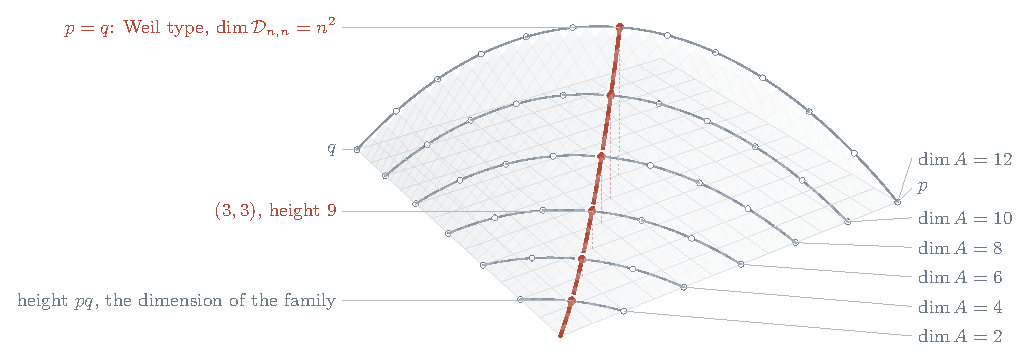
\includegraphics[width=0.92\textwidth]{fig_signature}
\caption{The signatures $(p,q)$ of an imaginary quadratic action, with
$p+q=\dim A$, drawn on the surface of height $pq$, which is the dimension of
the family of abelian varieties carrying that action, the unitary Shimura
variety of signature $(p,q)$. Each curve on the surface collects the
signatures available in one dimension, and on it the diagonal point is the
highest. The divisibility conditions of \Cref{thm:albert} put no
constraint on which of them occur when $\End^{0}(A)=K$, by
\Cref{prop:whichtypes}(i). By \Cref{prop:signatureforced} the Weil line
consists of Hodge classes exactly at the filled points on the ridge
$p=q$, and at every open point it is a rational sub-Hodge structure of type
$\{(p,2n-p),(2n-p,p)\}$ carrying no Hodge class at all. The diagonal is the
locus that \Cref{cor:weilalgebraic} shows to be an algebraic subvariety of the
moduli.}
\label{fig:albert}
\end{figure}

\subsection{The polarisation condition is automatic}

\begin{lemma}[Rosati on an imaginary quadratic subfield]\label{lem:rosatiauto}
Let $A$ be an abelian variety with a polarisation $\eta$ and Rosati involution
$\dagger$, and let $\iota\colon K\hookrightarrow\End^{0}(A)$ be an embedding of
an imaginary quadratic field such that $\iota(K)$ is stable under $\dagger$.
Then
\[
  \iota(\tau)^{\dagger}=\iota(\bbar{\tau})
  \qquad\text{for every }\tau\in K .
\]
That is, condition \textup{(iii)} of \Cref{def:weiltype} holds automatically,
and Weil type is the conjunction of \textup{(i)}, \textup{(ii)} and the
$\dagger$-stability of $\iota(K)$.
\end{lemma}

\begin{proof}
By stability, $\dagger$ restricts to a $\QQ$-algebra involution of the field
$\iota(K)\cong K$. A field automorphism of $K$ of order dividing two is either
the identity or complex conjugation, since $\Gal(K/\QQ)$ has order two and an
anti-automorphism of a commutative ring is an automorphism. Suppose it were
the identity, and put $x=\iota(\sqrt{-d})$. Then
$x\,x^{\dagger}=x^{2}=\iota(-d)=-d\cdot 1$, so
\[
  \Tr_{D/\QQ}\bigl(x\,x^{\dagger}\bigr)=-d\cdot\dim_{\QQ}D<0,
\]
contradicting positivity of $\dagger$. Hence $\dagger$ restricts to complex
conjugation.
\end{proof}

\begin{remark}\label{rem:whystable}
Stability is a genuine hypothesis and not a triviality: an arbitrary
subfield of $\End^{0}(A)$ need not be $\dagger$-stable. What
\Cref{lem:rosatiauto} removes is the second half of the condition, the
identification of $\dagger|_{K}$ with the specific automorphism. In
particular, in the model of \Cref{setup:model} one does not have to choose the
polarisation to match the field; any $\dagger$-stable embedding does the same
work.
\end{remark}

\subsection{The signature, and why balance is forced}

\begin{definition}[Signature]\label{def:signature}
Let $\iota\colon K\hookrightarrow\End^{0}(A)$ be as above, $g=\dim A$. The
operator $\iota(\sqrt{-d})$ acts on the tangent space $T_{0}A\cong\CC^{g}$ with
the two eigenvalues $\pm i\sqrt{d}$; write $p$ and $q=g-p$ for their
multiplicities. The pair $(p,q)$ is the \emph{signature} of $(A,\iota)$.
\end{definition}



The signature is an isogeny invariant, since an isogeny induces an isomorphism
on tangent spaces commuting with the action, and it is locally constant in
families, being the dimension of a kernel of a fixed operator on a bundle. By
duality $\iota(\tau)^{*}$ acts on $H^{1,0}(A)$ with the same multiplicities, so
$\dim V^{1,0}_{+}=p$ and $\dim V^{1,0}_{-}=q$ in the notation of
\Cref{sec:weiltype}.

\begin{proposition}[The balanced signature is forced]\label{prop:signatureforced}
Let $A$ be an abelian variety of dimension $2n$ with a $\dagger$-stable
embedding $\iota\colon K\hookrightarrow\End^{0}(A)$ of signature $(p,q)$,
$p+q=2n$, and let
\[
  \HW(A)=\Bigl(\textstyle\bigwedge^{2n}_{\CC}V_{+}
   \oplus\bigwedge^{2n}_{\CC}V_{-}\Bigr)\cap H^{2n}(A,\QQ)
\]
as in \Cref{def:weilline}. Then $\HW(A)$ is a rational sub-Hodge structure of
$H^{2n}(A,\QQ)$ of dimension two and of Hodge type
$\{(p,2n-p),\,(2n-p,p)\}$, and the following are equivalent:
\begin{enumerate}[label=\textup{(\roman*)},nosep]
\item $p=q=n$, that is $(A,\iota,\eta)$ is of $(K,-1,n)$-Weil type;
\item $\HW(A)$ contains a nonzero Hodge class;
\item $\HW(A)$ consists of Hodge classes.
\end{enumerate}
\end{proposition}

\begin{proof}
The space $\bigwedge^{2n}V_{+}$ is a line, and by \eqref{eq:bisplit} it equals
$\bigwedge^{p}V^{1,0}_{+}\otimes\bigwedge^{2n-p}V^{0,1}_{+}$, which is of pure
Hodge bidegree $(p,2n-p)$; the conjugate line $\bigwedge^{2n}V_{-}$ is of
bidegree $(2n-p,p)$. Their sum is stable under conjugation and defined over
$\QQ$ by the argument of \Cref{prop:weilline}(i), which never used the
balanced condition, so $\HW(A)$ is a two-dimensional rational sub-Hodge
structure of the stated type.

A Hodge class is an element of bidegree $(n,n)$. A nonzero element of
$\HW(A)\otimes\CC$ has a nonzero component in one of the two lines, so it is of
bidegree $(n,n)$ only if $(p,2n-p)=(n,n)$ or $(2n-p,p)=(n,n)$, both of which
say $p=n$. This gives (ii) implies (i). If $p=n$ then both lines are of
bidegree $(n,n)$ and every element of $\HW(A)$ is a Hodge class, which is (i)
implies (iii); and (iii) implies (ii) because $\dim\HW(A)=2>0$.
\end{proof}

\begin{remark}\label{rem:onlybalanced}
\Cref{prop:signatureforced} is the reason the literature speaks of abelian
varieties of Weil type rather than of imaginary quadratic multiplication in
general. For an unbalanced signature the space $\HW(A)$ still exists, is still
a canonical two-dimensional rational sub-Hodge structure, and is still not in
the divisor subring, but it contains no Hodge class and therefore predicts
nothing. The exceptional Hodge classes appear exactly at balance, and the
locus of balance is the algebraic subvariety of \Cref{cor:weilalgebraic}. The
statement is verified over all signatures $p$ and all $n\le3$ in
\texttt{explicit\_weil.py}, check (W4).
\end{remark}

\subsection{Which algebras can carry Weil classes}

\begin{proposition}[Weil type in the classification]\label{prop:whichtypes}
Let $A$ be an abelian variety of dimension $2n$ admitting a $\dagger$-stable
embedding of an imaginary quadratic field $K$ with balanced signature, and
suppose $\End^{0}(A)$ is a division algebra $D$ with centre $F$ as in
\Cref{thm:albert}. Then:
\begin{enumerate}[label=\textup{(\roman*)},nosep]
\item if $D=K$ then $D$ is of type IV with $e_{0}=1$ and $d=1$, and the
  divisibility condition of \Cref{thm:albert} is vacuous, so every even
  dimension occurs;
\item $D$ can also be of type III with $F_{0}=\QQ$, since a totally definite
  quaternion algebra over $\QQ$ contains imaginary quadratic subfields on which
  the canonical involution is conjugation;
\item $D$ cannot be of type I unless $D\subsetneq\End^{0}(A)$, because a
  totally real field contains no imaginary quadratic subfield.
\end{enumerate}
\end{proposition}

\begin{proof}
(i) If $D=K$ then $F=K$ is a CM field with $F_{0}=\QQ$, so $e_{0}=1$; and
$[D:F]=1$ gives $d=1$. The involution is conjugation by
\Cref{lem:rosatiauto}, which is type IV. The condition $e_{0}d^{2}\mid g$ reads
$1\mid 2n$.

(ii) Let $D$ be a quaternion algebra over $\QQ$ ramified at the infinite place,
with standard generators $u,v$ satisfying $u^{2}=a<0$, $v^{2}=b<0$, $uv=-vu$,
and canonical involution $x\mapsto\bbar{x}$ fixing $\QQ$ and negating
$u,v,uv$. Then $\QQ(u)\cong\QQ(\sqrt{a})$ is imaginary quadratic, stable under
the involution, and the involution restricts to conjugation on it. Whether
such a $D$ actually occurs as $\End^{0}(A)$ together with a balanced signature
is a separate question about the moduli, but nothing in the classification
excludes it.

(iii) Immediate, a totally real field has no element of negative square.
\end{proof}

\begin{remark}[The generic case is the one that matters]\label{rem:genericcase}
Case (ii) of \Cref{prop:whichtypes} is a special position: there
$\End^{0}(A)$ is larger than $K$, the Hodge group is correspondingly smaller,
and $\Hdg^{n}(A)$ can be larger than the three dimensions of
\Cref{thm:hdgcount}. It also tends to be the case where the Weil classes are
accessible; \Cref{rem:special} records that at such points the Weil line can
meet the divisor subring, which is the split situation. The hard case, and the
one all of \Cref{sec:divisor,sec:characters,sec:hyperplane} address, is
case (i) with $\Hg(A)=\SU(V,H)$.
\end{remark}

\begin{remark}[Why dimension four is where the subject starts]\label{rem:dimfour}
For $n=1$ the Weil line lies in $H^{2}(A,\QQ)$ and consists of divisor
classes, algebraic by the Lefschetz theorem on $(1,1)$ classes, so it predicts
nothing new; this is the same boundary as in \Cref{prop:normpart}. Moonen and
Zarhin determined the Hodge classes on abelian varieties of dimension at most
five \cite{MZ99}, and on simple abelian fourfolds in \cite{MZ95}: through
dimension three the Hodge ring is generated by divisor classes, and the first
Hodge classes not of that form occur in dimension four, on abelian fourfolds of
Weil type. So $n=2$ is simultaneously the first case of
\Cref{def:weiltype} with anything in it, the first case where
\Cref{thm:hdgcount} gives three rather than one, and the case that was the
first open one of the Hodge conjecture for abelian varieties until Markman
settled it \cite[Corollary 1.6.1]{Mar25a}; the first open case is now $n=3$
at nontrivial discriminant, by \Cref{prop:separate}(ii).
\end{remark}

\section{The verification script}\label{app:scripts}

The output below is the first part of a run of \texttt{verify\_all.py}, and
covers items (I) to (V) of \Cref{sec:verification}; the remaining items are
carried by the companion scripts named there, and the whole run ends with the
line \texttt{947 checks passed, 0 failed}. Everything requires the standard library of Python~3,
together with \texttt{sympy} for \texttt{secant\_plane.py} and
\texttt{weiltype\_family.py}, where it does exact symbolic linear algebra over
$\QQ(\sqrt{-d})$, for \texttt{mumford\_rigidity.py}, where it factors
Gram determinants over $\QQ[a_{0},\dots,a_{3}]$, and for
\texttt{mumford\_object.py}, \texttt{lefschetz\_closure.py},
\texttt{twistor\_locus.py} and \texttt{hk\_pullback.py}, where it computes
exact ranks, null spaces, determinants and characteristic polynomials, and
\texttt{numpy} for \texttt{pte\_remaining.py} and \texttt{weil\_tori.py},
where it holds integer arrays and reduces them modulo a prime; no step uses
floating point.

\begin{small}
\begin{verbatim}
(I) the Fourier-Mukai transform on powers of the polarisation
  [PASS] g=1: every image is a pure multiple of theta^(g-k)
  [PASS] g=2: every image is a pure multiple of theta^(g-k)
         k=0: -1/2  k=1: 1  k=2: -2
  [PASS] g=3: multiples agree with the closed form
         k=0: 1/6  k=1: -1/2  k=2: 2  k=3: -6
  [PASS] g=4: multiples agree with the closed form
         k=0: 1/24  k=1: -1/6  k=2: 1  k=3: -6  k=4: 24

(II) the sign sigma(g,k), uniform over index sets
  [PASS] sign is the same for every index set T, all g <= 12
  [PASS] sign equals (-1)^(g(g+1)/2 + k), all g <= 12

(III) the character grading: Weil line against eta^n
  [PASS] Weil line and eta^n occupy different summands, 1 <= n <= 4
         n=2: Weil line at (r,s) = [(4,0), (0,4)],  eta^2 at (2,2)
         n=3: Weil line at (r,s) = [(6,0), (0,6)],  eta^3 at (3,3)
  [PASS] the characters tau^(2n) and N^n are never equal for n >= 1

(IV) the secant count against the Lefschetz thresholds
  [PASS] 2n^2+2n < 2^(2n) < 3^(2n) for 2 <= n <= 8
         n=2: chi required 12,  2^(2n) 16,  3^(2n) 81
         n=3: chi required 24,  2^(2n) 64,  3^(2n) 729
  [PASS] counterexample: (1,3) is base point free with chi = 3 < 4
  [PASS] counterexample: (1,5) is very ample with chi = 5 < 9
  [PASS] so neither threshold is a necessary condition

(V) the semiregularity target
  [PASS] sum_q h^(q,q+2) = C(4n,2n-2) for 2 <= n <= 7
         n=2: 28    n=3: 495   n=4: 8008   n=5: 125970
  [PASS] the target grows by a factor above 10 at each step

  18 checks passed, 0 failed
  overall: PASS
\end{verbatim}
\end{small}

Item (XXI), the existence of a sheaf with the required Chern character, is the
one item whose output is an explicit witness rather than a verdict, so we
reproduce the dimension four block of \texttt{secant\_exists.py} as well.

\begin{small}
\begin{verbatim}
  == n = 4 ==
       d=3, a=1, b=1:  M = 6,
       alpha = -23[O(0t)] + 66[O(1t)] - 54[O(2t)] + 20[O(3t)] - 3[O(4t)]
       rank alpha = 6 = M a
  [PASS] n=4: the Vandermonde system is solvable for every (d,a,b)
  [PASS] n=4: every witness reproduces M c_k in every degree
  [PASS] n=4: every witness has rank exactly M a > 0
  [PASS] n=4: the multiple M is bounded over the whole range
         largest M = 12, and M = 1 in 4 of 72 cases
  [PASS] n=4: theta^k/k! has integer coefficients in a symplectic basis
\end{verbatim}
\end{small}

Item (XXXIII), the closure graph, is the other item whose output is worth
reading rather than merely passing, since it is the statement of what is left.
The block below is the frontier it computes, over the rules of this paper and
those of \Cref{ssec:bullseye}, followed by the derivation it prints for each
minimal sufficient set.

\begin{small}
\begin{verbatim}
  [PASS] the minimal sufficient sets are enumerated exhaustively
         5 of them, over the 16 open statements, from 65536 subsets
  [PASS] the minimal sufficient sets are exactly five
         {red_ab}, {lef_B, mot}, {lef_B, red_ab_mod}, {red_ab_mod, vhc}
         and {P2_cm_s, red_ab_mod, red_weil}
  [PASS] exactly one single open statement suffices, and it is red_ab
         the conjecture for the varieties that are not abelian gives the
         conjecture for abelian varieties through A x P^1, and then the
         conjecture
  [PASS] the route through this paper and the two routes of the
         literature with red_ab suffice and are not minimal
         each contains the sufficient singleton {red_ab}; with
         red_ab_mod in its place each is minimal
  [PASS] red_ab_mod alone gives neither the conjecture for abelian
         varieties nor the conjecture
         it holds trivially on abelian varieties, so it needs a second
         statement that reaches them
  [PASS] the route through this paper, with red_ab_mod, is the only
         minimal sufficient set with three elements
         it needs one statement more than each route of the literature
         through red_ab_mod

       the minimal sufficient sets:
            {red_ab}
            {lef_B, mot}
            {lef_B, red_ab_mod}
            {red_ab_mod, vhc}
            {P2_cm_s, red_ab_mod, red_weil}
       with
            P2_cm_s        (P2) for the split Weil families of the CM
                           fields of degree at least four
            lef_B          the Lefschetz standard conjecture B(X) for
                           every smooth complex projective variety X
            mot            every Hodge class on every smooth complex
                           projective variety is motivated in the sense
                           of Andre
            red_ab         the Hodge conjecture for every smooth
                           projective variety that is not an abelian
                           variety; equivalent to the conjecture, since
                           it covers A x P^1 for every abelian variety A
                           (prop:f3ishc)
            red_ab_mod     every Hodge class on every smooth projective
                           variety is algebraic modulo images of Hodge
                           classes of abelian varieties under algebraic
                           correspondences (def:f3prime); trivial on
                           abelian varieties
            red_weil       every Hodge class on an abelian variety
                           outside the subring generated by divisor
                           classes and Weil classes of quotients is
                           algebraic; not a reduction, since the self-
                           product of a Mumford fourfold carries two
                           such classes
            vhc            a global section of R^{2p} f_* Q for a smooth
                           projective family over a smooth connected
                           base that is algebraic at one point is
                           algebraic at every point

  [PASS] every member of a minimal sufficient set other than P2_cm_s is
         a consequence of the conjecture
         lef_B by thm:equivalence, mot by prop:lefmot, vhc by
         prop:lefvhc, red_ab_mod by prop:f3prime, red_ab and red_weil
         directly; no implication from the conjecture to P2 is known
  [PASS] {red_ab} and {lef_B, mot} are equivalences with the conjecture
         {red_ab} by prop:f3ishc, {lef_B, mot} by prop:lefmot
  [PASS] every minimal sufficient set contains red_ab, red_ab_mod or mot
         the varieties that are not abelian are reached only through the
         conjecture for them, through the conjecture modulo abelian
         varieties, or through motivated classes
  [PASS] the variational statement alone gives the conjecture for
         abelian varieties and not the conjecture
         so it covers the Weil classes of every CM field and the classes
         beyond the Weil lines at once
  [PASS] the Lefschetz standard conjecture gives the variational
         statement
         through the deformation theorem for motivated classes
  [PASS] only the route through this paper uses a statement proved in it
         the four other minimal sets rest on open statements and quoted
         theorems alone
  [PASS] each element of a minimal sufficient set is necessary to it
         removing any one of them leaves the conjecture underivable
  [PASS] the secant route lies in no minimal sufficient set
         granting all six of its open demands does not put it on a path
         to the conjecture
  [PASS] the secant route, fully granted, reaches every imaginary
         quadratic family and stops short of the fields of higher degree
         its base points are split members, of trivial discriminant, and
         descent (prop:descent) carries the trivial discriminant to
         every other; it has no base point over a field of degree at
         least four
  [PASS] the trivial discriminant closes the imaginary quadratic case
         by descent: B x Y, with Y a Weil surface of any discriminant,
         and a push-forward against the Weil class of Y
  [PASS] the split families of the fields of degree at least four close
         the imaginary quadratic case as well
         by scalar extension B -> B (x) O_F, every K lying in K(sqrt 2)
  [PASS] the propagation statement for the split imaginary quadratic
         families closes the imaginary quadratic case outright
         a base point exists in every split family, and descent does the
         rest
  [PASS] the propagation statement for the split families of the fields
         of degree at least four closes the Weil classes of every CM
         field
         descent within each field, and scalar extension down to the
         imaginary quadratic fields
  [PASS] the families of nontrivial discriminant need no propagation
         statement of their own
         no minimal sufficient set contains (P2) for a family of
         nontrivial discriminant or for an imaginary quadratic field
  [PASS] the bounded criterion (P1) is not in the rule set
         it is equivalent to the conjecture for the family, so it is a
         restatement and not a premise
  [PASS] the Weil classes of the higher CM fields are derived, not open
  [PASS] without prop:f3ishc and red_ab_mod the search returns the four
         sets of the earlier version
         {lef_B, mot}, {lef_B, red_ab}, {red_ab, vhc}, {P2_cm_s, red_ab,
         red_weil}: the change is those two additions, with (P2) read on
         the split families of the higher fields
  [PASS] the rule of prop:f3ishc has red_ab as its only premise
         and the conjecture for abelian varieties as its conclusion: the
         conjecture for A x P^1 gives it for A

       the conjecture from the proved and quoted statements and red_ab
            HC_ab         from red_ab
                                                             [prop:f3ishc]
            HC            from HC_ab, red_ab
                                                         [ssec:closuremap]

       the conjecture from the proved and quoted statements and lef_B,
         mot
            HC            from lef_B, mot
                                                             [prop:lefmot]

       the conjecture from the proved and quoted statements and lef_B,
         red_ab_mod
            vhc           from lef_B, mot_def
                                                             [prop:lefvhc]
            HC_ab         from vhc, acc_ab
                                                               [thm:vhcab]
            HC            from HC_ab, red_ab_mod
                                                            [prop:f3prime]

       the conjecture from the proved and quoted statements and
         red_ab_mod, vhc
            HC_ab         from vhc, acc_ab
                                                               [thm:vhcab]
            HC            from HC_ab, red_ab_mod
                                                            [prop:f3prime]

       the conjecture from the proved and quoted statements and P2_cm_s,
         red_ab_mod, red_weil
            weil_cm_triv  from base_point_cm, reduction_cm,
                               orbit_dense_cm, P2_cm_s
                                                       [thm:cmpropagation]
            weil_cm_nontriv from weil_cm_triv
                                                            [prop:descent]
            weil_triv     from weil_cm_triv
                                                            [prop:descent]
            weil_cm       from weil_cm_triv, weil_cm_nontriv
                                                             [prop:cmweil]
            weil_nontriv  from weil_triv
                                                            [prop:descent]
            weil_iq       from weil_triv, weil_nontriv
                                                           [prop:separate]
            weil_all      from weil_iq, weil_cm
                                                              [app:albert]
            HC_ab         from weil_all, red_weil
                                                         [ssec:closuremap]
            HC            from HC_ab, red_ab_mod
                                                            [prop:f3prime]
\end{verbatim}
\end{small}

Item (XLI) prints the numbers on which \Cref{thm:mumfordks} turns: the
scalar $\nu$, the transport of the real multiplication, and the shape of the
Kuga--Satake map on the explicit Clifford algebra.

\begin{small}
\begin{verbatim}
  [PASS] mu mu^dagger acts on each U_ij by one and the same nonzero
         rational nu
         nu = -1 on U_12, U_13, U_23; 27/2 on the line of theta
  [PASS] with kappa = e and the form q_lambda, mu mu^dagger acts on U_ij
         by nu g_i g_j, where g = e^2/lambda
         e = (2, -1, 5), lambda = (3, 7, 2): on U_ij by nu g_i g_j,
         g = (4/3, 1/7, 25/2)
  [PASS] kappa^dagger kappa, for the trace form on End(V), is
         multiplication by 4 e^2/lambda
  [PASS] C^+(T) has dimension 256 and is V^{32}: the vectors of highest
         weight (1,1,1) span 32 dimensions, and lowering them gives a basis
         dim C^+ = 256, highest weight vectors 32
  [PASS] N_1, N_2, N_3 anticommute pairwise and each squares to a nonzero
         scalar, proportional to the conjugate of lambda
         N_i^2 = 4, 8, 20 for lambda = (1, 2, 5)
\end{verbatim}
\end{small}

Item (XLIV) prints the checks behind \Cref{thm:mumfordrigid} and
\Cref{thm:mumfordnumerical}: the weight blocks, the factors of their Gram
determinants, the one kernel vector, and the certificates.

\begin{small}
\begin{verbatim}
  [PASS] wedge^2 V splits as 1 + 9 + 9 + 9 and the four tensors pi are
         invariant
         dimensions {'0': 1, '12': 9, '13': 9, '23': 9}
  [PASS] sp^{-1,1} has dimension 36, split into nine weight blocks
         block dimensions {(-2, -2): 3, (-2, 0): 4, (-2, 2): 3, (0,
         -2): 4, (0, 0): 8, (0, 2): 4, (2, -2): 3, (2, 0): 4, (2, 2):
         3}
  [PASS] the generic kernel is one vector, in the block of weight (0,0),
         and it does not depend on a
         the tangent direction of the Mumford curve
  [PASS] every Gram determinant is a positive constant times a product of
         P1, P2, Q1, Q2, Q3, Q4 and a2^2 + a3^2
  [PASS] each of the seven forms is a sum of squares of rational linear
         forms with positive coefficients
  [PASS] the common zeros of the squared linear forms of each form have
         two of a1, a2, a3 equal
         so for pairwise distinct a1, a2, a3 every block has full rank
         and the tangent space is one dimensional
  [PASS] tangent dimensions: 1 for distinct coefficients, 10 for a1 = a2
         = a3, 20 for a0 = a1 = a2 = a3
         computed 1, 10, 20
  [PASS] the annihilator in HH^2 (dimension 120) of an exceptional class
         is one dimensional at forty random admissible points, and 36
         dimensional for the class with equal coefficients
         so on a nonempty Zariski open set of classes, which contains
         rational ones, the least dimension of Ext^2 is 119
  [PASS] the annihilator does jump on special loci, which contain no
         rational exceptional class
         dimension 7 at a2 = 0 and 4 on the hyperplane a0 - 3 a1 - 3 a2
         + a3 = 0
  [PASS] HH^2 = H^{0,2} + H^1(T) + H^0(wedge^2 T) splits into blocks by
         type, weight and exchange parity, and omega_a is exchange
         invariant
         dimensions {'pi': 28, 'v': 64, 'z': 28}
  [PASS] every block Gram determinant is a positive constant times a
         product of P1, P2, Q1..Q4, R, S1..S4, Z1..Z6, a2, a3, L0, L1,
         L2, L3
  [PASS] the only block with a kernel at a generic point is the exchange
         even block of weight (0,0) of H^1(T), its kernel is independent
         of a and is the derivation of the Mumford curve
  [PASS] L0 = a0 + a1 + a2 + a3 divides only the Gram determinants of the
         exchange odd blocks of bivectors
         9 blocks
  [PASS] S1..S4 are sums of squares whose zeros force two of a1, a2, a3
         to coincide or one to vanish; Z1..Z6 are positive definite, as
         sums of four squares of independent forms with positive
         coefficients
  [PASS] every linear factor other than L0 has unequal coefficients on
         a1, a2, a3
         so it does not vanish at the conjugates of an irrational
         element of a cubic field, whatever the rational a0
  [PASS] on the hyperplane L0 = 0 the annihilator has dimension 10
         at three sample points: [10, 10, 10]
\end{verbatim}
\end{small}

Item (XLV) prints the checks behind \Cref{thm:mumfordprofile} and
\Cref{prop:mumforddivisor}.

\begin{small}
\begin{verbatim}
  [PASS] the ranks of contraction into omega at (3,5,-7,11), exact over
         Q, are 1,16,119,328,560,328,119,16,1 in degrees 0..8
         computed [1, 16, 119, 328, 560, 328, 119, 16, 1]
  [PASS] they vanish in degrees above eight
  [PASS] the same ranks, modulo p = 1000133, at a0 = 2 and the conjugates
         of 2cos(2pi/7) in each of the six orders
         a rational exceptional class for the cubic subfield of
         Q(zeta_7)
  [PASS] on the hyperplane a0 + a1 + a2 + a3 = 0 the ranks drop to
         1,16,110,328,548,328,110,16,1
         computed [1, 16, 110, 328, 548, 328, 110, 16, 1]
  [PASS] for a random class with components of types (0,0) to (3,3) the
         ranks are palindromic, r_k = r_{8-k}, and zero above eight
         computed [1, 16, 104, 322, 474, 322, 104, 16, 1, 0, 0]
  [PASS] the alternating sum of the ranks is 112, and 2r_0 + 2r_2 + r_4 =
         800
         so chi(E,E) = 0 forces Ext^1 + Ext^3 >= 400 when Ext^{<0} = 0
  [PASS] at a CM point: 16 divisor classes, 132 Hodge classes in degree
         four, products of divisor classes spanning 100
  [PASS] the combinations of the pi in that span are exactly those with
         a1 = a2 = a3
         so no rational exceptional class is a polynomial in divisor
         classes at any point
  [PASS] at a CM point X_c has 4 divisor classes and 8 Hodge classes in
         degree four, of which products of divisors span 6
         the other two are not products of divisor classes
\end{verbatim}
\end{small}

Item (XLVI) prints the checks behind \Cref{thm:lefschetzclosure}.

\begin{small}
\begin{verbatim}
  [PASS] the 36 maps lie in sp(V, psi), there are 32 root vectors, and
         the Lie algebra of G lies in sp(V, psi)
  [PASS] the Sp(V, psi)-invariants of wedge^k(V+V) have dimension
         1,3,6,10,15,10,6,3,1, and the products of the three invariant
         divisor classes span them
         upper [1, 3, 6, 10, 15, 10, 6, 3, 1],
         lower [1, 3, 6, 10, 15, 10, 6, 3, 1]
  [PASS] the G-invariants have dimension 1,3,8,16,28,16,8,3,1 (by
         weight multiplicities, and as the kernel modulo p), so the
         Hodge classes that are not Lefschetz number 0,0,2,6,13,6,2,0,0,
         29 in all
         computed [1, 3, 8, 16, 28, 16, 8, 3, 1]
  [PASS] at a CM point the T_Sp-invariant monomials number
         1,16,100,304,454,304,100,16,1 = coefficients of (1+4y+y^2)^4,
         each a product of the 16 divisor classes, which span exactly
         them
         Hodge classes [1, 16, 132, 432, 648, 432, 132, 16, 1]
  [PASS] at a CM point the Hodge classes number
         1,16,132,432,648,432,132,16,1
  [PASS] pi_0 and pi_12 + pi_13 + pi_23 are Sp-invariant and pi_12 is
         not; omega_a is T_Sp-invariant exactly when a1 = a2 = a3
         12 monomials of nonzero T_Sp-weight, exact rank 2
  [PASS] the module generated by pi_12 - pi_13, and the one generated by
         pi_13 - pi_23, has dimension 308 and highest weight (2,2,0,0)
         dimensions [308, 308]
  [PASS] Weyl's formula for Sp_8: dimensions 1, 27, 42, 308 for 0, w_2,
         w_4, 2w_2, and 1 + 27 + 42 + 308 = 378 = 27*28/2
  [PASS] that module meets the span of the four pi in a plane: the
         exceptional plane
         computed [2, 2]
\end{verbatim}
\end{small}

Item (XLVII) prints the checks behind \Cref{prop:notwistor}.

\begin{small}
\begin{verbatim}
  [PASS] s = s_1 (x) s_2 (x) s_3 is a real structure, V_R has real
         dimension 8, and psi is real and alternating on V_R
  [PASS] J_3, J_1, J_2 preserve V_R and square to -1; psi(x, Jy) is real
         symmetric of signature (0,8) for J_3 and (4,4) for J_1 and J_2
         signatures {'J_3': (0, 8, 0), 'J_1': (4, 4, 0),
         'J_2': (4, 4, 0)}
  [PASS] at J_1 the quaternion k = s_1 (x) 1 (x) 1 preserves V_R and
         psi, anticommutes with J_1 and carries psi(x, J_1 y) to its
         negative; so psi (x) S is congruent to its negative, hence
         indefinite, for every nonzero real symmetric 2 x 2 matrix S: no
         invariant class of degree two polarises the square
         signature (m,m) confirmed directly on 6 matrices S
  [PASS] at J_1 the tensors pi have type (2,2) and the annihilator of
         omega_a in H^1(T) (dimension 64) is spanned by the lowering
         derivation of the first factor on both copies
         dimension 64, kernel 1
  [PASS] at J_3, the Mumford family, it is spanned by the lowering
         derivation of the third factor, as in item (XLIV)
         dimension 64, kernel 1
  [PASS] the exchange of the first and third factors carries pi_12 to
         pi_23 and fixes pi_0 and pi_13
\end{verbatim}
\end{small}

Item (XLVIII) prints the checks behind \Cref{prop:hksquare}.

\begin{small}
\begin{verbatim}
  [PASS] iota(x) = (x (x) 1) Psi is symmetric for the nine generators of
         T, and y.iota(x) = iota([y, x]) for all pairs of generators
  [PASS] the Casimirs split H^2 of the square (dimension 120) into
         isotypic pieces of dimensions 3, 27, 27, 27, 27, 3, 3, 3 with
         (2,0)-parts 0, 0, 9, 9, 9, 0, 0, 1; the pieces of types
         (2,0,0), (0,2,0), (0,0,2) are iota(T_1), iota(T_2), iota(T_3),
         and only the Galois orbit of T has h^{2,0} = 1
         dims [3, 27, 27, 27, 27, 3, 3, 3]
  [PASS] sigma_0 = iota(E_3) is of type (2,0) and pairs the
         (1,0)-vectors of the two copies through an invertible 4 x 4
         block, so it is a holomorphic symplectic form on the square
         det of the block 1
  [PASS] iota_2(C_1) = 3 pi_0 - pi_12 - pi_13 + 3 pi_23 and cyclically;
         so iota_2(sum s_i C_i) = omega_a with a_0 = 3 sum s_i and
         a_ij = 4 s_k - sum s_i
  [PASS] det(x_1 + x_2 + x_3 on V) = Delta(N_1, N_2, N_3)^2 with N_i =
         -det(x_i), as a polynomial identity in nine variables
  [PASS] iota(x)^8 = +- 8! det(x) vol at sample points, with one sign
         ratios [1, 1, 1]
  [PASS] Delta is a nondegenerate ternary quadratic form (Gram
         determinant -4) and irreducible, so Delta(N)^2 is not a
         constant multiple of the fourth power of a linear form
         Gram determinant -4
\end{verbatim}
\end{small}

Item (XLIX) prints the checks behind \Cref{cor:mumfordone} and
\Cref{rem:mumfordneeded}.

\begin{small}
\begin{verbatim}
  [PASS] every theorem label in the rule set is a label of the paper,
         and every statement named in a rule is declared
         22 rules, 11 labels
  [PASS] the target is not in the closure of the proved statements
  [PASS] the statements equivalent to the target over the proved ones
         are exactly TARGET, UNCOUNT, B_WW, BOUND and MODP
         ['BOUND', 'B_WW', 'MODP', 'TARGET', 'UNCOUNT']
  [PASS] every minimal set of open statements yielding the target has
         one element, so one route suffices
         12 minimal sets: BOUND, B_WW, EXT119, F2, F3, HC, HK_U, KS_U,
         L, MODP, UNCOUNT, V
  [PASS] the target yields none of EXT119, KS_U, HK_U: those routes are
         stronger than the target, not forms of it
  [PASS] L and V each yield the target, so on the routes to the
         conjecture through them the target is not an input
  [PASS] HC and F2 yield the target, and the target yields none of HC,
         F1, F2, F3, L, V, M
  [PASS] F3 is equivalent to HC and is itself a one-element route to the
         target
         by prop:f3ishc; so the three statements of cor:fourremain are
         not three obligations either
  [PASS] the minimal sets of open statements yielding HC in this rule
         set are {HC}, {F3} and {L, M}, and none contains the target
         {F3}, {HC}, {L, M}
\end{verbatim}
\end{small}

The source is distributed with the paper as \texttt{verify\_all.py}. Its four
substantive routines are an exterior algebra over $\QQ$ with basis elements
indexed by bit masks and the shuffle sign \eqref{eq:shufflesign}; the
transform $\Phi_{\cP}$ implemented as multiplication by $e^{\ell}$ followed by
extraction of the coefficient of the top form in the dual variables; the
permutation sign of \Cref{lem:appsign}; and the binomial identities of
\Cref{prop:target}. No step uses floating point.


\section*{Declarations}

\subsection*{Funding}
None.

\subsection*{Competing interests}
None.


\begin{thebibliography}{99}

\bibitem[Alb34]{Alb34}
A. A. Albert,
\emph{On the construction of Riemann matrices. I},
Ann. of Math. (2) \textbf{35} (1934), no.~1, 1--28.
\href{https://doi.org/10.2307/1968116}{\texttt{doi:10.2307/1968116}}.

\bibitem[Alb35a]{Alb35a}
A. A. Albert,
\emph{On the construction of Riemann matrices. II},
Ann. of Math. (2) \textbf{36} (1935), no.~2, 376--394.
\href{https://doi.org/10.2307/1968578}{\texttt{doi:10.2307/1968578}}.

\bibitem[Alb35b]{Alb35b}
A. A. Albert,
\emph{Involutorial simple algebras and real Riemann matrices},
Ann. of Math. (2) \textbf{36} (1935), no.~4, 886--964.
\href{https://doi.org/10.2307/1968595}{\texttt{doi:10.2307/1968595}}.

\bibitem[And92]{And92}
Y. Andr\'e,
\emph{Mumford--Tate groups of mixed Hodge structures and the theorem of the
fixed part},
Compositio Math. \textbf{82} (1992), no.~1, 1--24.
\href{http://www.numdam.org/item/CM_1992__82_1_1_0/}{\texttt{numdam.org/item/CM\_1992\_\_82\_1\_1\_0}}.

\bibitem[And96a]{And96}
Y. Andr\'e,
\emph{On the Shafarevich and Tate conjectures for hyperk\"ahler varieties},
Math. Ann. \textbf{305} (1996), no.~2, 205--248.
\href{https://doi.org/10.1007/BF01444219}{\texttt{doi:10.1007/BF01444219}}.

\bibitem[And96b]{And96b}
Y. Andr\'e,
\emph{Pour une th\'eorie inconditionnelle des motifs},
Inst. Hautes \'Etudes Sci. Publ. Math. \textbf{83} (1996), 5--49.
\href{https://doi.org/10.1007/BF02698643}{\texttt{doi:10.1007/BF02698643}}.

\bibitem[BB66]{BB66}
W. L. Baily, Jr. and A. Borel,
\emph{Compactification of arithmetic quotients of bounded symmetric domains},
Ann. of Math. (2) \textbf{84} (1966), no.~3, 442--528.
\href{https://doi.org/10.2307/1970457}{\texttt{doi:10.2307/1970457}}.

\bibitem[Bea83]{Bea83}
A. Beauville,
\emph{Vari\'et\'es K\"ahleriennes dont la premi\`ere classe de Chern est
nulle},
J. Differential Geom. \textbf{18} (1983), no.~4, 755--782.
\href{https://doi.org/10.4310/jdg/1214438181}{\texttt{doi:10.4310/jdg/1214438181}}.

\bibitem[BF03]{BF03}
R.-O. Buchweitz and H. Flenner,
\emph{A semiregularity map for modules and applications to deformations},
Compositio Math. \textbf{137} (2003), no.~2, 135--210.
\href{https://doi.org/10.1023/A:1023999012081}{\texttt{doi:10.1023/A:1023999012081}}.

\bibitem[BF08]{BF08}
R.-O. Buchweitz and H. Flenner,
\emph{The global decomposition theorem for Hochschild (co-)homology of
singular spaces via the Atiyah--Chern character},
Adv. Math. \textbf{217} (2008), no.~1, 243--281.
\href{https://doi.org/10.1016/j.aim.2007.06.013}{\texttt{doi:10.1016/j.aim.2007.06.013}}.

\bibitem[BLM23]{BLM23}
R. Bandiera, E. Lepri and M. Manetti,
\emph{$L_{\infty}$ liftings of semiregularity maps via Chern--Simons classes},
Adv. Math. \textbf{435} (2023), 109358.
\href{https://doi.org/10.1016/j.aim.2023.109358}{\texttt{doi:10.1016/j.aim.2023.109358}}.
arXiv:2111.12985.

\bibitem[BL04]{BL04}
C. Birkenhake and H. Lange,
\emph{Complex Abelian Varieties}, 2nd ed.,
Grundlehren der mathematischen Wissenschaften \textbf{302},
Springer, Berlin, 2004.
\href{https://doi.org/10.1007/978-3-662-06307-1}{\texttt{doi:10.1007/978-3-662-06307-1}}.

\bibitem[BEK14]{BEK14}
S. Bloch, H. Esnault and M. Kerz,
\emph{$p$-adic deformation of algebraic cycle classes},
Invent. Math. \textbf{195} (2014), 673--722.
\href{https://doi.org/10.1007/s00222-013-0461-4}{\texttt{doi:10.1007/s00222-013-0461-4}}.

\bibitem[BS94]{BS94}
S. Bando and Y.-T. Siu,
\emph{Stable sheaves and Einstein--Hermitian metrics},
in: Geometry and Analysis on Complex Manifolds,
World Sci. Publ., River Edge, NJ, 1994, pp.~39--50.
\href{https://doi.org/10.1142/9789814350112_0002}{\texttt{doi:10.1142/9789814350112\_0002}}.

\bibitem[Blo72]{Blo72}
S. Bloch,
\emph{Semi-regularity and de Rham cohomology},
Invent. Math. \textbf{17} (1972), 51--66.
\href{https://doi.org/10.1007/BF01390023}{\texttt{doi:10.1007/BF01390023}}.

\bibitem[Bus19]{Bus19}
N. Buskin,
\emph{Every rational Hodge isometry between two K3 surfaces is algebraic},
J. Reine Angew. Math. \textbf{755} (2019), 127--150.
\href{https://doi.org/10.1515/crelle-2017-0027}{\texttt{doi:10.1515/crelle-2017-0027}}.

\bibitem[Cal05]{Cal05}
A. C\u{a}ld\u{a}raru,
\emph{The Mukai pairing, II: the Hochschild--Kostant--Rosenberg isomorphism},
Adv. Math. \textbf{194} (2005), no.~1, 34--66.
\href{https://doi.org/10.1016/j.aim.2004.05.012}{\texttt{doi:10.1016/j.aim.2004.05.012}}.

\bibitem[CDK95]{CDK95}
E. Cattani, P. Deligne and A. Kaplan,
\emph{On the locus of Hodge classes},
J. Amer. Math. Soc. \textbf{8} (1995), no.~2, 483--506.
\href{https://doi.org/10.1090/S0894-0347-1995-1273413-2}{\texttt{doi:10.1090/S0894-0347-1995-1273413-2}}.

\bibitem[CKS86]{CKS86}
E. Cattani, A. Kaplan and W. Schmid,
\emph{Degeneration of Hodge structures},
Ann. of Math. (2) \textbf{123} (1986), no.~3, 457--535.
\href{https://doi.org/10.2307/1971333}{\texttt{doi:10.2307/1971333}}.

\bibitem[CRV12]{CRV12}
D. Calaque, C. A. Rossi and M. Van den Bergh,
\emph{C\u{a}ld\u{a}raru's conjecture and Tsygan's formality},
Ann. of Math. (2) \textbf{176} (2012), no.~2, 865--923.
\href{https://doi.org/10.4007/annals.2012.176.2.4}{\texttt{doi:10.4007/annals.2012.176.2.4}}.

\bibitem[Del71]{Del71}
P. Deligne,
\emph{Th\'eorie de Hodge. II},
Inst. Hautes \'Etudes Sci. Publ. Math. \textbf{40} (1971), 5--57.
\href{https://doi.org/10.1007/BF02684692}{\texttt{doi:10.1007/BF02684692}}.

\bibitem[Del72]{Del72}
P. Deligne,
\emph{La conjecture de Weil pour les surfaces $K3$},
Invent. Math. \textbf{15} (1972), 206--226.
\href{https://doi.org/10.1007/BF01404126}{\texttt{doi:10.1007/BF01404126}}.

\bibitem[Del74]{Del74}
P. Deligne,
\emph{La conjecture de Weil. I},
Inst. Hautes \'Etudes Sci. Publ. Math. \textbf{43} (1974), 273--307.
\href{https://doi.org/10.1007/BF02684373}{\texttt{doi:10.1007/BF02684373}}.

\bibitem[Del82]{Del82}
P. Deligne,
\emph{Hodge cycles on abelian varieties} (notes by J. S. Milne),
in: Hodge Cycles, Motives, and Shimura Varieties,
Lecture Notes in Math. \textbf{900}, Springer, Berlin, 1982, pp.~9--100.
\href{https://doi.org/10.1007/978-3-540-38955-2_3}%
{\texttt{doi:10.1007/978-3-540-38955-2\_3}}.

\bibitem[FM98]{FM98}
B. Fantechi and M. Manetti,
\emph{Obstruction calculus for functors of Artin rings, I},
J. Algebra \textbf{202} (1998), no.~2, 541--576.
\href{https://doi.org/10.1006/jabr.1997.7239}{\texttt{doi:10.1006/jabr.1997.7239}}.

\bibitem[FF26]{FF26}
S. Floccari and L. Fu,
\emph{The Hodge conjecture for Weil fourfolds with discriminant $1$ via
singular OG6-varieties},
J. Math. Pures Appl. (9) \textbf{210} (2026), paper no.~103876.
\href{https://doi.org/10.1016/j.matpur.2026.103876}{\texttt{doi:10.1016/j.matpur.2026.103876}}.

\bibitem[Flo24]{Flo24}
S. Floccari,
\emph{Sixfolds of generalized Kummer type and K3 surfaces},
Compos. Math. \textbf{160} (2024), no.~2, 388--410.
\href{https://doi.org/10.1112/S0010437X23007625}{\texttt{doi:10.1112/S0010437X23007625}}.

\bibitem[Fuj87]{Fuj87}
A. Fujiki,
\emph{On the de Rham cohomology group of a compact K\"ahler symplectic
manifold},
in: Algebraic Geometry, Sendai, 1985, Adv. Stud. Pure Math. \textbf{10}
(1987), 105--165.
\href{https://doi.org/10.2969/aspm/01010105}{\texttt{doi:10.2969/aspm/01010105}}.

\bibitem[Ful98]{Ful98}
W. Fulton,
\emph{Intersection Theory}, 2nd ed.,
Ergebnisse der Mathematik und ihrer Grenzgebiete (3) \textbf{2},
Springer, New York, 1998.
\href{https://doi.org/10.1007/978-1-4612-1700-8}{\texttt{doi:10.1007/978-1-4612-1700-8}}.

\bibitem[Gal00]{Gal00}
F. Galluzzi,
\emph{Abelian fourfold of Mumford-type and Kuga--Satake varieties},
Indag. Math. (N.S.) \textbf{11} (2000), no.~4, 547--560.
\href{https://doi.org/10.1016/S0019-3577(00)80024-5}{\texttt{doi:10.1016/S0019-3577(00)80024-5}}.

\bibitem[GM88]{GM88}
W. M. Goldman and J. J. Millson,
\emph{The deformation theory of representations of fundamental groups of
compact K\"ahler manifolds},
Inst. Hautes \'Etudes Sci. Publ. Math. \textbf{67} (1988), 43--96.
\href{https://doi.org/10.1007/BF02699127}{\texttt{doi:10.1007/BF02699127}}.

\bibitem[GP98]{GP98}
M. Gross and S. Popescu,
\emph{Equations of $(1,d)$-polarized abelian surfaces},
Math. Ann. \textbf{310} (1998), no.~2, 333--377.
\href{https://doi.org/10.1007/s002080050151}{\texttt{doi:10.1007/s002080050151}}.

\bibitem[Gri10]{Gri10}
J. Grivaux,
\emph{Chern classes in Deligne cohomology for coherent analytic sheaves},
Math. Ann. \textbf{347} (2010), no.~2, 249--284.
\href{https://doi.org/10.1007/s00208-009-0430-9}{\texttt{doi:10.1007/s00208-009-0430-9}}.

\bibitem[Gro61]{Gro61}
A. Grothendieck,
\emph{Techniques de construction et th\'eor\`emes d'existence en g\'eom\'etrie
alg\'ebrique IV: les sch\'emas de Hilbert},
S\'eminaire Bourbaki, Vol.~6 (1960/61), Exp. No.~221, 249--276;
reprinted by Soc. Math. France, Paris, 1995.

\bibitem[HM73]{HM73}
G. Horrocks and D. Mumford,
\emph{A rank $2$ vector bundle on $\mathbf{P}^{4}$ with $15{,}000$ symmetries},
Topology \textbf{12} (1973), 63--81.
\href{https://doi.org/10.1016/0040-9383(73)90022-0}{\texttt{doi:10.1016/0040-9383(73)90022-0}}.

\bibitem[Hua21]{Hua21}
S. Huang,
\emph{A note on a question of Markman},
J. Pure Appl. Algebra \textbf{225} (2021), no.~9, 106673.
\href{https://doi.org/10.1016/j.jpaa.2021.106673}{\texttt{doi:10.1016/j.jpaa.2021.106673}}.

\bibitem[Huy16]{Huy16}
D. Huybrechts,
\emph{Lectures on K3 Surfaces},
Cambridge Studies in Advanced Mathematics \textbf{158},
Cambridge University Press, Cambridge, 2016.
\href{https://doi.org/10.1017/CBO9781316594193}{\texttt{doi:10.1017/CBO9781316594193}}.

\bibitem[Kle68]{Kle68}
S. L. Kleiman,
\emph{Algebraic cycles and the Weil conjectures},
in: Dix expos\'es sur la cohomologie des sch\'emas,
North-Holland, Amsterdam, 1968, pp.~359--386.

\bibitem[Kle94]{Kle94}
S. L. Kleiman,
\emph{The standard conjectures},
in: Motives (Seattle, WA, 1991),
Proc. Sympos. Pure Math. \textbf{55}, Part 1,
Amer. Math. Soc., Providence, RI, 1994, pp.~3--20.
\href{https://doi.org/10.1090/pspum/055.1/1265519}{\texttt{doi:10.1090/pspum/055.1/1265519}}.

\bibitem[KS67]{KS67}
M. Kuga and I. Satake,
\emph{Abelian varieties attached to polarized $K3$-surfaces},
Math. Ann. \textbf{169} (1967), 239--242.
\href{https://doi.org/10.1007/BF01399540}{\texttt{doi:10.1007/BF01399540}}.

\bibitem[Kur65]{Kur65}
M. Kuranishi,
\emph{New proof for the existence of locally complete families of complex
structures},
in: Proc. Conf. Complex Analysis (Minneapolis, 1964),
Springer, Berlin, 1965, pp.~142--154.
\href{https://doi.org/10.1007/978-3-642-48016-4_13}{\texttt{doi:10.1007/978-3-642-48016-4\_13}}.

\bibitem[Li26]{Li26}
N. Li,
\emph{The Tate conjecture for powers of abelian fourfolds and the Hodge
conjecture for powers of CM fourfolds},
preprint, 2026.
\href{https://arxiv.org/abs/2609.27916}{\texttt{arXiv:2609.27916}}.

\bibitem[Lie06]{Lie06}
M. Lieblich,
\emph{Moduli of complexes on a proper morphism},
J. Algebraic Geom. \textbf{15} (2006), no.~1, 175--206.
\href{https://doi.org/10.1090/S1056-3911-05-00418-2}%
{\texttt{doi:10.1090/S1056-3911-05-00418-2}}.

\bibitem[Mar25a]{Mar25a}
E. Markman,
\emph{Cycles on abelian $2n$-folds of Weil type from secant sheaves on abelian
$n$-folds}, preprint, arXiv:2502.03415 (2025).
\href{https://doi.org/10.48550/arXiv.2502.03415}{\texttt{doi:10.48550/arXiv.2502.03415}}.

\bibitem[Mar25b]{Mar25b}
E. Markman,
\emph{Secant sheaves and Weil classes on abelian varieties},
preprint, arXiv:2509.23403 (2025).
\href{https://doi.org/10.48550/arXiv.2509.23403}{\texttt{doi:10.48550/arXiv.2509.23403}}.

\bibitem[Mat86]{Mat86}
H. Matsumura,
\emph{Commutative Ring Theory},
Cambridge Studies in Advanced Mathematics \textbf{8},
Cambridge University Press, Cambridge, 1986.
\href{https://doi.org/10.1017/CBO9781139171762}{\texttt{doi:10.1017/CBO9781139171762}}.

\bibitem[Mil20]{Mil20}
J. S. Milne,
\emph{Hodge classes on abelian varieties},
preprint, 2020.
\href{https://arxiv.org/abs/2010.08857}{\texttt{arXiv:2010.08857}}.

\bibitem[Mil22]{Mil22}
J. S. Milne,
\emph{The Tate and standard conjectures for certain abelian varieties},
preprint, arXiv:2112.12815, version 2 (2022).
\href{https://doi.org/10.48550/arXiv.2112.12815}{\texttt{doi:10.48550/arXiv.2112.12815}}.

\bibitem[Mor84]{Mor84}
D. R. Morrison,
\emph{On K3 surfaces with large Picard number},
Invent. Math. \textbf{75} (1984), no.~1, 105--121.
\href{https://doi.org/10.1007/BF01403093}{\texttt{doi:10.1007/BF01403093}}.

\bibitem[Mor19]{Mor19}
M. Morrow,
\emph{A variational Tate conjecture in crystalline cohomology},
J. Eur. Math. Soc. \textbf{21} (2019), no.~11, 3467--3511.
\href{https://doi.org/10.4171/JEMS/907}{\texttt{doi:10.4171/JEMS/907}}.

\bibitem[Muk78]{Muk78}
S. Mukai,
\emph{Semi-homogeneous vector bundles on an abelian variety},
J. Math. Kyoto Univ. \textbf{18} (1978), no.~2, 239--272.
\href{https://doi.org/10.1215/kjm/1250522574}{\texttt{doi:10.1215/kjm/1250522574}}.

\bibitem[Muk81]{Muk81}
S. Mukai,
\emph{Duality between $D(X)$ and $D(\hat{X})$ with its application to Picard
sheaves},
Nagoya Math. J. \textbf{81} (1981), 153--175.
\href{https://doi.org/10.1017/S002776300001922X}{\texttt{doi:10.1017/S002776300001922X}}.

\bibitem[Mum69]{Mum69}
D. Mumford,
\emph{A note of Shimura's paper ``Discontinuous groups and abelian
varieties''},
Math. Ann. \textbf{181} (1969), 345--351.
\href{https://doi.org/10.1007/BF01350672}{\texttt{doi:10.1007/BF01350672}}.

\bibitem[MZ95]{MZ95}
B. Moonen and Yu. G. Zarhin,
\emph{Hodge classes and Tate classes on simple abelian fourfolds},
Duke Math. J. \textbf{77} (1995), no.~3, 553--581.
\href{https://doi.org/10.1215/S0012-7094-95-07717-5}{\texttt{doi:10.1215/S0012-7094-95-07717-5}}.

\bibitem[MZ99]{MZ99}
B. Moonen and Yu. G. Zarhin,
\emph{Hodge classes on abelian varieties of low dimension},
Math. Ann. \textbf{315} (1999), no.~4, 711--733.
\href{https://doi.org/10.1007/s002080050333}{\texttt{doi:10.1007/s002080050333}}.

\bibitem[OMe00]{OMe00}
O. T. O'Meara,
\emph{Introduction to Quadratic Forms},
Classics in Mathematics, Springer, Berlin, 2000 (reprint of the 1973 edition).
\href{https://doi.org/10.1007/978-3-642-62031-7}{\texttt{doi:10.1007/978-3-642-62031-7}}.

\bibitem[Per26]{Per26}
A. Perry,
\emph{The semiregularity theorem for equivariant noncommutative varieties},
preprint, arXiv:2604.00511 (2026).
\href{https://doi.org/10.48550/arXiv.2604.00511}{\texttt{doi:10.48550/arXiv.2604.00511}}.

\bibitem[PR94]{PR94}
V. P. Platonov and A. S. Rapinchuk,
\emph{Algebraic Groups and Number Theory},
Pure and Applied Mathematics \textbf{139},
Academic Press, Boston, MA, 1994.

\bibitem[Pri24]{Pri24}
J. P. Pridham,
\emph{Semiregularity as a consequence of Goodwillie's theorem},
Forum Math. Sigma \textbf{12} (2024), e126. arXiv:1208.3111.
\href{https://doi.org/10.1017/fms.2024.132}{\texttt{doi:10.1017/fms.2024.132}}.

\bibitem[Sat66]{Sat66}
I. Satake,
\emph{Clifford algebras and families of abelian varieties},
Nagoya Math. J. \textbf{27} (1966), 435--446.
\href{https://doi.org/10.1017/S0027763000026295}{\texttt{doi:10.1017/S0027763000026295}}.

\bibitem[Sch10]{Sch10}
U. Schlickewei,
\emph{The Hodge conjecture for self-products of certain K3 surfaces},
J. Algebra \textbf{324} (2010), no.~3, 507--529.
\href{https://doi.org/10.1016/j.jalgebra.2010.04.010}{\texttt{doi:10.1016/j.jalgebra.2010.04.010}}.

\bibitem[Sch73]{Sch73}
W. Schmid,
\emph{Variation of Hodge structure: the singularities of the period mapping},
Invent. Math. \textbf{22} (1973), 211--319.
\href{https://doi.org/10.1007/BF01389674}{\texttt{doi:10.1007/BF01389674}}.

\bibitem[Sch85]{Sch85}
W. Scharlau,
\emph{Quadratic and Hermitian Forms},
Grundlehren der mathematischen Wissenschaften \textbf{270},
Springer, Berlin, 1985.
\href{https://doi.org/10.1007/978-3-642-69971-9}{\texttt{doi:10.1007/978-3-642-69971-9}}.

\bibitem[Ser00]{Ser00}
J.-P. Serre,
\emph{Local Algebra},
Springer Monographs in Mathematics,
Springer, Berlin, 2000.
\href{https://doi.org/10.1007/978-3-662-04203-8}{\texttt{doi:10.1007/978-3-662-04203-8}}.

\bibitem[SGA\,$4\frac{1}{2}$]{SGA4h}
P. Deligne,
\emph{Cohomologie \'etale} (SGA $4\frac{1}{2}$), with the expos\'e
[Cycle], \emph{La classe de cohomologie associ\'ee \`a un cycle}, by
A. Grothendieck, r\'edig\'e par P. Deligne, pp.~129--153,
Lecture Notes in Math. \textbf{569}, Springer, Berlin, 1977.
\href{https://doi.org/10.1007/BFb0091516}{\texttt{doi:10.1007/BFb0091516}}.

\bibitem[Stacks]{Stacks}
The Stacks project authors,
\emph{The Stacks project},
\href{https://stacks.math.columbia.edu}{\texttt{https://stacks.math.columbia.edu}},
2026.

\bibitem[Tan03]{Tan03}
S. G. Tankeev,
\emph{On the standard conjecture for complex abelian schemes over smooth
projective curves},
Izv. Math. \textbf{67} (2003), no.~3, 597--635.
\href{https://doi.org/10.1070/IM2003v067n03ABEH000439}{\texttt{doi:10.1070/IM2003v067n03ABEH000439}}.

\bibitem[Tod09]{Tod09}
Y. Toda,
\emph{Deformations and Fourier--Mukai transforms},
J. Differential Geom. \textbf{81} (2009), no.~1, 197--224.
\href{https://doi.org/10.4310/jdg/1228400631}{\texttt{doi:10.4310/jdg/1228400631}}.

\bibitem[Tot26]{Tot26}
B. Totaro,
\emph{On the Hodge conjecture},
guest post on the weblog of T. Tao, 11 September 2026.
\href{https://terrytao.wordpress.com/2026/09/11/on-the-hodge-conjecture/}%
{\texttt{terrytao.wordpress.com/2026/09/11/on-the-hodge-conjecture}}.

\bibitem[Var23]{Var23}
M. Varesco,
\emph{Hodge similarities, algebraic classes, and Kuga--Satake varieties},
Math. Z. \textbf{305} (2023), paper no.~69.
\href{https://doi.org/10.1007/s00209-023-03390-8}{\texttt{doi:10.1007/s00209-023-03390-8}}.

\bibitem[vG00]{vG00}
B. van Geemen,
\emph{Kuga--Satake varieties and the Hodge conjecture},
in: The Arithmetic and Geometry of Algebraic Cycles (Banff, 1998),
NATO Sci. Ser. C Math. Phys. Sci. \textbf{548},
Kluwer, Dordrecht, 2000, pp.~51--82.
\href{https://doi.org/10.1007/978-94-011-4098-0_3}{\texttt{doi:10.1007/978-94-011-4098-0\_3}}.

\bibitem[vG08]{vG08}
B. van Geemen,
\emph{Real multiplication on K3 surfaces and Kuga Satake varieties},
Michigan Math. J. \textbf{56} (2008), no.~2, 375--399.
\href{https://doi.org/10.1307/mmj/1224783519}{\texttt{doi:10.1307/mmj/1224783519}}.

\bibitem[vGR26]{vGR26}
B. van Geemen and A. Rapagnetta,
\emph{Hyperk\"ahler sixfolds, abelian fourfolds of Weil type and a Hodge
class},
preprint, 2026.
\href{https://arxiv.org/abs/2607.18341}{\texttt{arXiv:2607.18341}}.

\bibitem[vGS25]{vGS25}
B. van Geemen and M. Sch\"utt,
\emph{On families of K3 surfaces with real multiplication},
Forum Math. Sigma \textbf{13} (2025), Paper No. e2.
\href{https://doi.org/10.1017/fms.2024.146}{\texttt{doi:10.1017/fms.2024.146}}.

\bibitem[Voi02]{Voi02}
C. Voisin,
\emph{Hodge Theory and Complex Algebraic Geometry I},
Cambridge Studies in Advanced Mathematics \textbf{76},
Cambridge University Press, Cambridge, 2002.
\href{https://doi.org/10.1017/CBO9780511615344}{\texttt{doi:10.1017/CBO9780511615344}}.

\bibitem[Voi02b]{Voi02b}
C. Voisin,
\emph{A counterexample to the Hodge conjecture extended to K\"ahler
varieties},
Int. Math. Res. Not. \textbf{2002}, no.~20, 1057--1075.
\href{https://doi.org/10.1155/S1073792802111135}{\texttt{doi:10.1155/S1073792802111135}}.
\href{https://arxiv.org/abs/math/0112247}{\texttt{arXiv:math/0112247}}.

\bibitem[Voi03]{Voi03}
C. Voisin,
\emph{Hodge Theory and Complex Algebraic Geometry II},
Cambridge Studies in Advanced Mathematics \textbf{77},
Cambridge University Press, Cambridge, 2003.
\href{https://doi.org/10.1017/CBO9780511615177}{\texttt{doi:10.1017/CBO9780511615177}}.

\bibitem[Voi26]{Voi26}
C. Voisin,
\emph{The status of the Hodge conjecture},
guest post on the weblog of T. Tao, 12 September 2026.
\href{https://terrytao.wordpress.com/2026/09/12/the-status-of-the-hodge-conjecture/}%
{\texttt{terrytao.wordpress.com/2026/09/12/the-status-of-the-hodge-conjecture}}.

\bibitem[Wei77]{Weil77}
A. Weil,
\emph{Abelian varieties and the Hodge ring},
in: \OE uvres Scientifiques, Collected Papers, Vol.~III,
Springer, New York, 1979, pp.~421--429.

\bibitem[Zhu18]{Zhu18}
Y. Zhu,
\emph{K3 surfaces associated to abelian fourfolds of Mumford's type},
preprint, arXiv:1812.06882 (2018).
\href{https://doi.org/10.48550/arXiv.1812.06882}{\texttt{doi:10.48550/arXiv.1812.06882}}.

\bibitem[Zuc79]{Zuc79}
S. Zucker,
\emph{Hodge theory with degenerating coefficients: $L_{2}$ cohomology in the
Poincar\'e metric},
Ann. of Math. (2) \textbf{109} (1979), no.~3, 415--476.
\href{https://doi.org/10.2307/1971221}{\texttt{doi:10.2307/1971221}}.

\end{thebibliography}


\end{document}
